%%
%%

\documentclass[11pt,a4paper]{book}
%\usepackage{html}
\usepackage{float}
\usepackage{graphicx}
\usepackage{bacula}
\usepackage{longtable}
\usepackage{makeidx}
\usepackage{index}
\usepackage{setspace}
\usepackage{hyperref}


\makeindex
\newindex{dir}{ddx}{dnd}{Director Index}
\newindex{fd}{fdx}{fnd}{File Daemon Index}
\newindex{sd}{sdx}{snd}{Storage Daemon Index}
\newindex{console}{cdx}{cnd}{Console Index}
\newindex{general}{idx}{ind}{General Index}

\sloppy

\begin{document}
\sloppy

\newfont{\bighead}{cmr17 at 36pt}
\parskip 10pt
\parindent 0pt

\title{
\includegraphics{./bacula-logo.eps} \\ \bigskip
  \begin{center}
   \large{It comes in the night and sucks 
          the essence from your computers. }
  \end{center}
}
\author{Kern Sibbald}
\date{\vspace{2.0in} 21 April 2005 \\
      This manual documents Bacula version 1.36.3 \\
      Copyright \copyright 1999-2005, Kern Sibbald }

\maketitle

\clearpage
\tableofcontents
\clearpage
\listoffigures
\clearpage
\listoftables
\clearpage

%%
%%

\section*{What is Bacula?}
\label{_ChapterStart41}
\index[general]{Bacula!What is }
\index[general]{What is Bacula? }
\addcontentsline{toc}{section}{What is Bacula?}

{\bf Bacula} is a set of computer programs that permit you (or the system
administrator) to manage backup, recovery, and verification of computer data
across a network of computers of different kinds. In technical terms, it is a
network Client/Server based backup program. Bacula is relatively easy to use
and efficient, while offering many advanced storage management features that
make it easy to find and recover lost or damaged files. Due to its modular
design, Bacula is scalable from small single computer systems to systems
consisting of hundreds of computers located over a large network. 

\subsection*{Who Needs Bacula?}
\index[general]{Who Needs Bacula? }
\index[general]{Bacula!Who Needs }
\addcontentsline{toc}{subsection}{Who Needs Bacula?}

If you are currently using a program such as {\bf tar}, {\bf dump}, or {\bf
bru} to backup your computer data, and you would like a network solution, more
flexibility, or catalog services, Bacula will most likely provide the
additional features you want. However, if you are new to Unix systems or do
not have offsetting experience with a sophisticated backup package, we do not
recommend using Bacula as it is much more difficult to setup and use than {\bf
tar} or {\bf dump}. 

If you are running {\bf Amanda} and would like a backup program that can write
to multiple volumes (i.e. is not limited by your tape drive capacity), Bacula
can most likely fill your needs. In addition, quite a number of our users
report that Bacula is simpler to setup and use than other equivalent programs.


If you are currently using a sophisticated commercial package such as Legato
Networker. ARCserveIT, Arkeia, or PerfectBackup+, you may be interested in
Bacula, which provides many of the same features, and is free software
available under the GNU Version 2 software license. 

\subsection*{Bacula Components or Services}
\index[general]{Bacula Components or Services }
\index[general]{Services!Bacula Components or }
\addcontentsline{toc}{subsection}{Bacula Components or Services}

Bacula is made up of the following five major components or services: 

\addcontentsline{lof}{figure}{Bacula Applications}
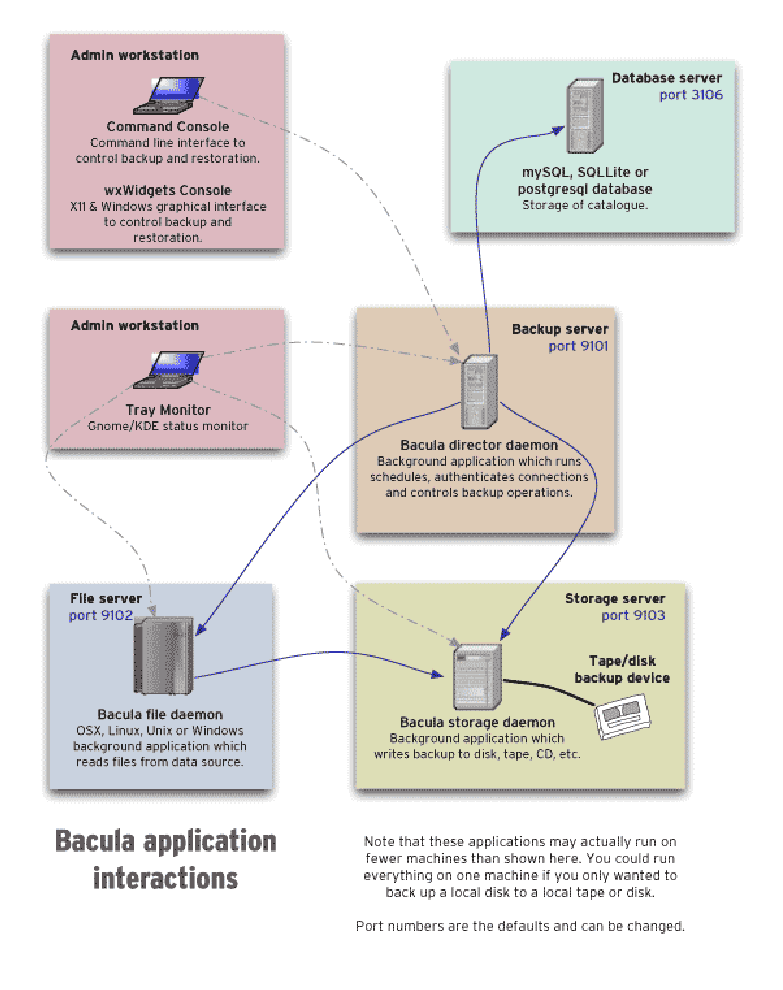
\includegraphics{./bacula-applications.eps} 
(thanks to Aristedes Maniatis for this graphic and the one below) 

\begin{itemize}
\item 
   \label{DirDef}
   {\bf Bacula Director} service consists of the program that  supervises all the
backup, restore, verify and archive operations.  The system administrator uses
the Bacula Director to schedule  backups and to recover files. For more
details see the  Director Services Daemon Design Document in the Bacula
Developer's  Guild.  The Director runs as a daemon or a service (i.e. in the
background). 
\item 
   \label{UADef}
   {\bf Bacula Console} services is the program that allows the  administrator or
user to communicate with the {\bf Bacula Director}  (see above). Currently,
the Bacula Console is available in three  versions. The first and simplest is
to run the Console program in a  shell window (i.e. TTY interface). Most
system administrators will  find this completely adequate. The second version
is a GNOME GUI  interface that for the moment (23 November 2003) is far from
complete,  but quite functional as it has most the capabilities of the shell 
Console. The third version is a wxWidgets GUI with an interactive file 
restore. It also has most the capabilities of the shell console,  allows
command completion with tabulation, and gives you instant  help about the
command you are typing. For more details see the  
\ilink{Bacula Console Design Document}{_ChapterStart23}. 
\item 
   \label{FDDef}
   {\bf Bacula File} services (or Client program) is the software  program that
is installed on the machine to be backed up. It is  specific to the operating
system on which it runs and is responsible  for providing the file attributes
and data when requested by the  Director. The File services are also
responsible for the file  system dependent part of restoring the file
attributes and data  during a recovery operation. For more details see the 
File Services Daemon Design Document in the Bacula Developer's Guide. This 
program runs as a daemon on the machine to be backed up, and in some  of the
documentation, the File daemon is referred to as the Client  (for example in
Bacula's configuration file). In addition to  Unix/Linux File daemons, there
is a Windows File daemon (normally  distributed in binary format). The Windows
File daemon runs on  all currently known Windows versions (95, 98, Me, NT,
2000, XP). 
\item 
   \label{SDDef}
   {\bf Bacula Storage} services consist of the software programs that  perform
the storage and recovery of the file attributes and data to  the physical
backup media or volumes. In other words, the Storage daemon  is responsible
for reading and writing your tapes (or other  storage media, e.g. files). For
more details see the  Storage Services Daemon Design Document in the Bacula
Developer's Guild.  The Storage services runs as a daemon on the machine that
has the  backup device (usually a tape drive). 
\item 
   \label{DBDefinition}
   {\bf Catalog} services are comprised of the software programs  responsible for
maintaining the file indexes and volume databases for  all files backed up.
The Catalog services permit the System  Administrator or user to quickly
locate and restore any desired  file. The Catalog services sets Bacula apart
from simple backup  programs like tar and bru, because the catalog maintains a
record  of all Volumes used, all Jobs run, and all Files saved, permitting 
efficicient restoration and Volume management.  Bacula currently supports
three different databases, MySQL,  PostgreSQL, and SQLite, one of which must
be chosen when building  {\bf Bacula}. There also exists an Internal database,
but it is no  longer supported.  

The three SQL databases currently supported (MySQL, PostgreSQL or SQLite) 
provide quite a number of features,  including rapid indexing, arbitrary
queries, and security. Although  we plan to support other major SQL databases,
the current  Bacula implementation interfaces only to MySQL, PostgreSQL and
SQLite.  For more details see the 
\ilink{Catalog Services Design Document}{_ChapterStart30}.  

The RPMs for MySQL and PostgreSQL ship as part of the Linux RedHat release, 
or building it from the source is quite easy, see the  
\ilink{ Installing and Configuring MySQL}{_ChapterStart} chapter  of
this document for the details. For more information on MySQL,  please see: 
\elink{www.mysql.com}{http://www.mysql.com}.  Or see the 
\ilink{ Installing and Configuring PostgreSQL}{_ChapterStart10}
chapter of this document for the details. For more  information on PostgreSQL,
please see: 
\elink{www.postgresql.org}{http://www.postgresql.org}.  

Configuring and building SQLite is even easier. For the details  of
configuring SQLite, please see the 
\ilink{ Installing and Configuring SQLite}{_ChapterStart33} chapter
of this document. 
\item 
   \label{MonDef}
   {\bf Bacula Monitor} services is the program that allows the  administrator or
user to watch current status of {\bf Bacula Directors},  {\bf Bacula File
Daemons} and {\bf Bacula Storage Daemons}  (see above). Currently, only a GTK+
version is available, which  works with Gnome and KDE (or any window manager
that supports the  FreeDesktop.org system tray standard). 
\end{itemize}

To perform a successful save or restore, the following four daemons must be
configured and running: the Director daemon, the File daemon, the Storage
daemon, and MySQL, PostgreSQL or SQLite. 

\subsection*{Bacula Configuration}
\index[general]{Configuration!Bacula }
\index[general]{Bacula Configuration }
\addcontentsline{toc}{subsection}{Bacula Configuration}

In order for Bacula to understand your system, what clients you want backed
up, and how, you must create a number of configuration files containing
resources (or objects). The following presents an overall picture of this: 

\addcontentsline{lof}{figure}{Bacula Objects}
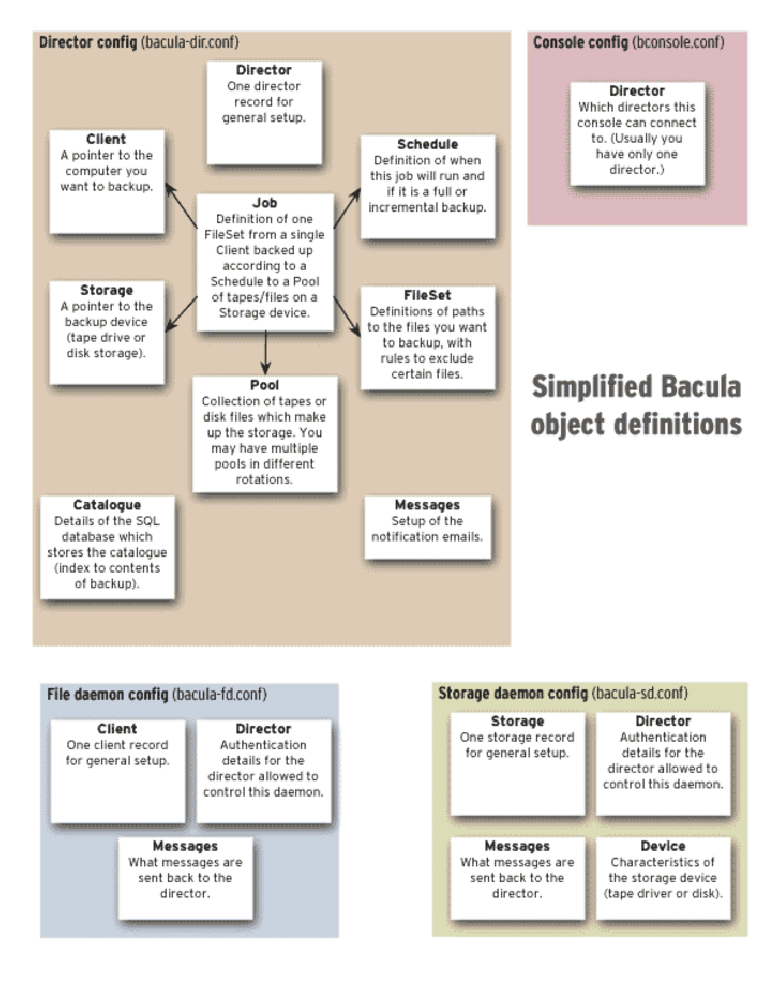
\includegraphics{./bacula-objects.eps} 

\subsection*{Conventions Used in this Document}
\index[general]{Conventions Used in this Document }
\index[general]{Document!Conventions Used in this }
\addcontentsline{toc}{subsection}{Conventions Used in this Document}

{\bf Bacula} is in a state of evolution, and as a consequence, this manual
will not always agree with the code. If an item in this manual is preceded by
an asterisk (*), it indicates that the particular feature is not implemented.
If it is preceded by a plus sign (+), it indicates that the feature may be
partially implemented. 

If you are reading this manual as supplied in a released version of the
software, the above paragraph holds true. If you are reading the online
version of the manual, 
\elink{ www.bacula.org/manual}{http://www.bacula.org/manual}, please bear in
mind that this version describes the current version in development (in the
CVS) that may contain features not in the released version. Just the same, it
generally lags behind the code a bit. 

\subsection*{Quick Start}
\index[general]{Quick Start }
\index[general]{Start!Quick }
\addcontentsline{toc}{subsection}{Quick Start}

To get Bacula up and running quickly, we recommend that you first scan the
Terminology section below, then quickly review the next chapter entitled 
\ilink{The Current State of Bacula}{_ChapterStart2}, then the 
\ilink{Getting Started with Bacula}{_ChapterStart37}, which will
give you a quick overview of getting Bacula running. After which, you should
proceed to the chapter on 
\ilink{Installing Bacula}{_ChapterStart17}, then 
\ilink{How to Configure Bacula}{_ChapterStart16}, and finally the
chapter on 
\ilink{ Running Bacula}{_ChapterStart1}. 

\subsection*{Terminology}
\index[general]{Terminology }
\addcontentsline{toc}{subsection}{Terminology}

To facilitate communication about this project, we provide here the
definitions of the terminology that we use. 

\begin{description}

\item [Administrator]
   \index[fd]{Administrator }
   The person or persons responsible for administrating  the Bacula system. 

\item [Backup]
   \index[fd]{Backup }
   We use the term {\bf Backup} to refer to a  Bacula Job that saves files. 

\item [Bootstrap File]
   \index[fd]{Bootstrap File }
   The bootstrap file is an ASCII file  containing a compact form of commands
that allow Bacula or  the stand-alone file extraction utility ({\bf bextract})
to  restore the contents of one or more Volumes, for example, the  current
state of a system just backed up. With a bootstrap file,  Bacula can restore
your system without a Catalog. You can  create a bootstrap file from a Catalog
to extract any file or  files you wish. 

\item [Catalog]
   \index[fd]{Catalog }
   The Catalog is used to store summary information  about the Jobs, Clients, and
Files that were backed up and on  what Volume or Volumes. The information
saved in the Catalog  permits the administrator or user to determine what jobs
were  run, their status as well as the important characteristics  of each file
that was backed up. The Catalog is an online resource,  but does not contain
the data for the files backed up. Most of  the information stored in the
catalog is also stored on the  backup volumes (i.e. tapes). Of course, the
tapes will also have  a copy of the file in addition to the File Attributes
(see below).  

The catalog feature is one part of Bacula that distinguishes  it from simple
backup and archive programs such as {\bf dump}  and {\bf tar}.  

\item [Client]
   \index[fd]{Client }
   In Bacula's terminology, the word Client  refers to the machine being backed
up, and it is synonymous  with the File services or File daemon, and quite
often, we  refer to it as the FD. A Client is defined in a configuration  file
resource. 

\item [Console]
   \index[fd]{Console }
   The program that interfaces to the Director allowing  the user or system
administrator to control Bacula. 

\item [Daemon]
   \index[fd]{Daemon }
   Unix terminology for a program that is always present in  the background to
carry out a designated task. On Windows systems, as  well as some Linux
systems, daemons are called {\bf Services}. 

\item [Directive]
   \index[fd]{Directive }
   The term directive is used to refer to a statement  or a record within a
Resource in a configuration file that  defines one specific thing. For
example, the {\bf Name} directive  defines the name of the Resource. 

\item [Director]
   \index[fd]{Director }
   The main Bacula server daemon that schedules and directs all  Bacula
operations. Occassionally, we refer to the Director as DIR. 

\item [Differential]
   \index[fd]{Differential }
   A backup that includes all files changed since the last  Full save started.
Note, other backup programs may define this differently. 

\item [File Attributes]
   \index[fd]{File Attributes }
   The File Attributes are all the information  necessary about a file to
identify it and all its properties such as  size, creation date, modification
date, permissions, etc. Normally, the  attributes are handled entirely by
Bacula so that the user never  needs to be concerned about them. The
attributes do not include the  file's data. 

\item [File Daemon]
   \index[fd]{File Daemon }
   The daemon running on the client  computer to be backed up. This is also
referred to as the File  services, and sometimes as the Client services or the
FD. 

\item [
   \label{FileSetDef}
   FileSet]
\index[fd]{a name }
A FileSet is a Resource contained in a configuration  file that defines the
files to be backed up. It consists  of a list of included files or
directories, a list of excluded files, and  how the file is to be stored
(compression, encryption, signatures).  For more details, see the 
\ilink{FileSet Resource definition}{FileSetResource}  in the
Director chapter of this document. 

\item [Incremental]
   \index[fd]{Incremental }
   A backup that includes all files changed since the  last Full, Differential,
or Incremental backup started. It is normally  specified on the {\bf Level}
directive within the Job resource  definition, or in a Schedule resourc. 

\item [
   \label{JobDef}
   Job]
\index[fd]{a name }
A Bacula Job is a configuration resource that defines  the work that Bacula
must perform to backup or restore a particular  Client. It consists of the
{\bf Type} (backup, restore, verify,  etc), the {\bf Level} (full,
incremental,...), the {\bf FileSet},  and {\bf Storage} the files are to be
backed up (Storage device,  Media Pool). For more details, see the 
\ilink{Job Resource definition}{JobResource} in the  Director
chapter of this document. 

\item [Monitor]
   \index[fd]{Monitor }
   The program that interfaces to the all the daemons  allowing the user or
system administrator to monitor Bacula status. 

\item [Resource]
   \index[fd]{Resource }
   A resource is a part of a configuration file that  defines a specific unit of
information that is available to Bacula.  For example, the {\bf Job} resource
defines all the properties of  a specific Job: name, schedule, Volume pool,
backup type, backup  level, ... 

\item [Restore]
   \index[fd]{Restore }
   A restore is a configuration resource that  describes the operation of
recovering a file (lost or damaged) from  backup media. It is the inverse of a
save, except that in most  cases, a restore will normally have a small set of
files to restore,  while normally a Save backs up all the files on the system.
Of  course, after a disk crash, Bacula can be called upon to do  a full
Restore of all files that were on the system. 

\item [Schedule]
   \index[fd]{Schedule }
   A Schedule is a configuration resource that  defines when the Bacula Job will
be scheduled for  execution. To use the Schedule, the Job resource will refer
to  the name of the Schedule. For more details, see the 
\ilink{Schedule Resource definition}{ScheduleResource} in the
Director chapter of this document. 

\item [Service]
   \index[fd]{Service }
   This is Windows terminology for a {\bf daemon} -- see  above. It is now
frequently used in Unix environments as well. 

\item [Storage Coordinates]
   \index[fd]{Storage Coordinates }
   The information returned from the  Storage Services that uniquely locates a
file on a backup medium. It  consists of two parts: one part pertains to each
file saved, and the  other part pertains to the whole Job. Normally, this
information is  saved in the Catalog so that the user doesn't need specific
knowledge  of the Storage Coordinates. The Storage Coordinates include the 
File Attributes (see above) plus the unique location of the information on 
the backup Volume. 

\item [Storage Daemon]
   \index[fd]{Storage Daemon }
   The Storage daemon, sometimes referred to as  the SD, is the code that writes
the attributes and data to a storage  Volume (usually a tape or disk). 

\item [Session]
   \index[sd]{Session }
   Normally refers to the internal conversation between  the File daemon and the
Storage daemon. The File daemon opens a  {\bf session} with the Storage daemon
to save a FileSet, or to restore  it. A session has a one to one
correspondence to a Bacula Job (see  above). 

\item [Verify]
   \index[sd]{Verify }
   A verify is a job that compares the current file  attributes to the attributes
that have previously been stored in the  Bacula Catalog. This feature can be
used for detecting changes to  critical system files similar to what {\bf
Tripwire} does. One  of the major advantages of using Bacula to do this is
that  on the machine you want protected such as a server, you can run  just
the File daemon, and the Director, Storage daemon, and Catalog  reside on a
different machine. As a consequence, if your server is  ever compromised, it
is unlikely that your verification database  will be tampered with.  

Verify can also be used to check that the most recent Job  data written to a
Volume agrees with what is stored in the Catalog  (i.e. it compares the file
attributes), *or it can check the  Volume contents against the original files
on disk. 

\item [*Archive]
   \index[fd]{*Archive }
   An Archive operation is done after a Save, and it  consists of removing the
Volumes on which data is saved from active  use. These Volumes are marked as
Archived, and many no longer be  used to save files. All the files contained
on an Archived Volume  are removed from the Catalog. NOT YET IMPLEMENTED. 

\item [*Update]
   \index[fd]{*Update }
   An Update operation causes the files on the remote  system to be updated to be
the same as the host system. This is  equivalent to an {\bf rdist} capability.
NOT YET IMPLEMENTED.  

\item [Retention Period]
   \index[fd]{Retention Period }
   There are various kinds of retention  periods that Bacula recognizes. The most
important are the  {\bf File} Retention Period, {\bf Job} Retention Period,
and the  {\bf Volume} Retention Period. Each of these retention periods 
applies to the time that specific records will be kept in the  Catalog
database. This should not be confused with the time that  the data saved to a
Volume is valid. 

The File Retention Period  determines the time that File records are kept in
the catalog  database. This period is important because the volume of the 
database File records by far use the most storage space in the  database. As a
consequence, you must ensure that regular  ``pruning'' of the database file
records is done. (See  the Console {\bf retention} command for more details on
this  subject). 

The Job Retention Period is the length of time that  Job records will be kept
in the database. Note, all the File  records are tied to the Job that saved
those files. The File  records can be purged leaving the Job records. In this
case,  information will be available about the jobs that ran, but not the 
details of the files that were backed up. Normally, when a Job  record is
purged, all its File records will also be purged. 

The  Volume Retention Period is the minimum of time that a Volume will be 
kept before it is reused. Bacula will normally never  overwrite a Volume that
contains the only backup copy of a file.  Under ideal conditions, the Catalog
would retain entries for all  files backed up for all current Volumes. Once a
Volume is  overwritten, the files that were backed up on that Volume are 
automatically removed from the Catalog. However, if there is a very  large
pool of Volumes or a Volume is never overwritten, the Catalog  database may
become enormous. To keep the Catalog to a manageable  size, the backup
information should removed from the Catalog after  the defined File Retention
Period. Bacula provides the  mechanisms for the catalog to be automatically
pruned according to  the retention periods defined. 

\item [Scan]
   \index[sd]{Scan }
   A Scan operation causes the contents of a Volume or a  series of Volumes to be
scanned. These Volumes with the information  on which files they contain are
restored to the Bacula Catalog.  Once the information is restored to the
Catalog, the files contained  on those Volumes may be easily restored. This
function is  particularly useful if certain Volumes or Jobs have exceeded 
their retention period and have been pruned or purged from the  Catalog.
Scanning data from Volumes into the Catalog is done  by using the {\bf bscan}
program. See the 
\ilink{ bscan section}{bscan} of the Bacula Utilities Chapter of
this manual  for more details. 

\item [Volume]
   \index[sd]{Volume }
   A Volume is an archive unit, normally a tape or  a named disk file where
Bacula stores the data from one or more  backup jobs. All Bacula Volumes have
a software label written to  the Volume by Bacula so that it identify what
Volume it is really  reading. (Normally there should be no confusion with disk
files,  but with tapes, it is easy to mount the wrong one). 
\end{description}

\subsection*{What Bacula is Not}
\index[general]{Not!What Bacula is }
\index[general]{What Bacula is Not }
\addcontentsline{toc}{subsection}{What Bacula is Not}

{\bf Bacula} is a backup, restore and verification program and is not a
complete disaster recovery system in itself, but it can be a key part of one
if you plan carefully and follow the instructions included in the 
\ilink{ Disaster Recovery}{_ChapterStart38} Chapter of this manual. 

With proper planning, as mentioned in the Disaster Recovery chapter {\bf
Bacula} can be a central component of your disaster recovery system. For
example, if you have created an emergency boot disk, a Bacula Rescue disk to
save the current partitioning information of your hard disk, and maintain a
complete Bacula backup, it is possible to completely recover your system from
``bare metal''. 

If you have used the {\bf WriteBootstrap} record in your job or some other
means to save a valid bootstrap file, you will be able to use it to extract
the necessary files (without using the catalog or manually searching for the
files to restore). 

\subsection*{Interactions Between the Bacula Services}
\index[general]{Interactions Between the Bacula Services }
\index[general]{Services!Interactions Between the Bacula }
\addcontentsline{toc}{subsection}{Interactions Between the Bacula Services}

The following block diagram shows the typical interactions between the Bacula
Services for a backup job. Each block represents in general a separate process
(normally a daemon). In general, the Director oversees the flow of
information. It also maintains the Catalog. 

\addcontentsline{lof}{figure}{Interactions between Bacula Services}
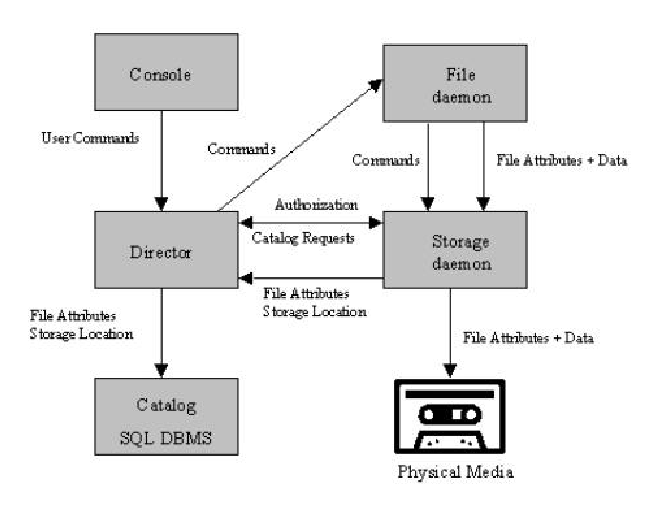
\includegraphics{./flow.eps} 

%%
%%

\section*{The Current State of Bacula}
\label{_ChapterStart2}
\index[general]{Current State of Bacula }
\addcontentsline{toc}{section}{Current State of Bacula}

In other words, what is and what is not currently implemented and functional. 

\subsection*{What is Implemented}
\index[general]{Implemented!What is }
\index[general]{What is Implemented }
\addcontentsline{toc}{subsection}{What is Implemented}

\begin{itemize}
\item Network backup/restore with centralized Director.  
\item Internal scheduler for automatic 
   \ilink{Job}{JobDef} execution.  
\item Scheduling of multiple Jobs at the same time.  
\item You may run one Job at a time or multiple simultaneous Jobs.  
\item Job sequencing using priorities.  
\item Restore of one or more files selected interactively either for  the
   current backup or a backup prior to a specified time and date.  
\item Restore of a complete system starting from bare  metal. This is mostly
   automated for Linux systems and  partially automated for Solaris. See 
   \ilink{Disaster Recovery Using Bacula}{_ChapterStart38}. This is also
   reported to work on Win2K/XP systems.  
\item Listing and Restoration of files using stand-alone {\bf bls} and  {\bf
   bextract} tool programs. Among other things, this permits  extraction of files
   when Bacula and/or the catalog are not  available. Note, the recommended way
   to restore files is using  the restore command in the Console. These programs
   are designed  for use as a last resort. 
\item Ability to recreate the catalog database by scanning backup Volumes 
   using the {\bf bscan} program.  
\item 
   \ilink{Console}{UADef} interface to the Director  allowing complete
   control. A shell, GNOME GUI and wxWidgets GUI versions of  the Console program
   are available. Note, the GNOME GUI program currently  offers very few
   additional features over the shell program. 
\item Verification of files previously cataloged, permitting a Tripwire like 
   capability (system break-in detection).  
\item CRAM-MD5 password authentication between each component (daemon).  
\item A comprehensive and extensible 
   \ilink{configuration file}{_ChapterStart40} for each daemon.  
\item Catalog database facility for remembering Volumes, Pools, Jobs,  and
   Files backed up.  
\item Support for SQLite, PostgreSQL, and MySQL Catalog databases.  
\item User extensible queries to the SQLite, PostgreSQL and MySQL databases.  
\item Labeled Volumes, preventing accidental overwriting  (at least by
   Bacula).  
\item Any number of Jobs and Clients can be backed up to a single  Volume.
   That is, you can backup and restore Linux, Unix, Sun, and  Windows machines to
   the same Volume.  
\item Multi-volume saves. When a Volume is full, {\bf Bacula}  automatically
   requests the next Volume and continues the backup.  
\item 
   \ilink{Pool and Volume}{PoolResource} library management 
   providing Volume flexibility (e.g. monthly, weekly, daily Volume sets,  Volume
   sets segregated by Client, ...). 
\item Machine independent Volume data format. Linux, Solaris, and Windows 
   clients can all be backed up to the same Volume if desired. 
\item A flexible 
   \ilink{ message}{MessageResource}  handler including routing
   of messages from any daemon back to the  Director and automatic email
   reporting.  
\item Multi-threaded implementation.  
\item Programmed to handle arbitrarily long filenames and messages.  
\item GZIP compression on a file by file basis done by the Client program  if
   requested before network transit.  
\item Computation of MD5 or SHA1 signatures of the file data if requested.  
\item Saves and restores POSIX ACLs if enabled.  
\item Autochanger support using a simple shell interface that can interface 
   to virtually any autoloader program. A script for {\bf mtx} is  provided.  
\item Support for autochanger barcodes -- automatic tape labeling from 
   barcodes.  
\item Automatic support for multiple autochanger magazines either using
   barcodes or by reading the tapes.  
\item Raw device backup/restore. Restore must be to the same device. 
\item All Volume blocks (approx 64K bytes) contain a data checksum.  
\item Access control lists for Consoles that permit restricting user  access
   to only their data.  
\item Data spooling to disk during backup with subsequent write to tape  from
   the spooled disk files. This prevents tape ``shoe shine''  during
   Incremental/Differential backups.  
\item Support for save/restore of files larger than 2GB.  
\item Support for 64 bit machines, e.g. amd64.  
\item Ability to encrypt communications between daemons using stunnel. 
   \end{itemize}

\subsection*{Advantages of Bacula Over Other Backup Programs}
\index[general]{Advantages of Bacula Over Other Backup Programs }
\index[general]{Programs!Advantages of Bacula Over Other Backup }
\addcontentsline{toc}{subsection}{Advantages of Bacula Over Other Backup
   Programs}

\begin{itemize}
\item Since there is a client for each machine, you can backup
   and restore clients of any type ensuring that all attributes
   of files are properly saved and restored.
\item It is also possible to backup clients without any client
   software by using NFS or Samba.  However, if possible, we
   recommend running a Client File daemon on each machine to be
   backed up.
\item Bacula handles multi-volume backups.  
\item A full comprehensive SQL standard database of all files backed up.  This
   permits online viewing of files saved on any particular  Volume.  
\item Automatic pruning of the database (removal of old records) thus 
   simplifying database administration.  
\item Any SQL database engine can be used making Bacula very flexible.  
\item The modular but integrated design makes Bacula very scalable.  
\item Since Bacula uses client file servers, any database or
   other application can be properly shutdown by Bacula using the
   native tools of the system, backed up, then restarted (all
   within a Bacula Job).
\item Bacula has a built-in Job scheduler.  
\item The Volume format is documented and there are simple C programs to 
   read/write it.  
\item Bacula uses well defined (registered) TCP/IP ports -- no rpcs,  no
   shared memory.  
\item Bacula installation and configuration is relatively simple compared  to
   other comparable products.  
\item According to one user Bacula is as fast as the big major commercial 
   application.  
\item According to another user Bacula is four times as fast as  another
   commercial application, probably because that application  stores its catalog
   information in a large number of individual  files rather than an SQL database
   as Bacula does.  
\item Aside from a GUI administrative interface, Bacula has a
   comprehensive shell administrative interface, which allows the
   adminstrator to use tools such as ssh to administrate any part of
   Bacula from anywhere (even from home).

\item Bacula has a Rescue CD for Linux systems with the following features:  
   \begin{itemize}
   \item You build it on your own system from scratch with one simple  command:
      make -- well, then make burn. 
   \item It uses your kernel  
   \item It captures your current disk parameters and builds scripts that  allow
      you to automatically repartition a disk and format it to  put it back to what
      you had before. 
   \item It has a script that will restart your networking (with the right  IP
      address)  
   \item It has a script to automatically mount your hard disks.  
   \item It has a full Bacula FD statically linked  
   \item You can easily add additional data/programs, ... to the disk.  
   \end{itemize}

\end{itemize}

\subsection*{Current Implementation Restrictions}
\index[general]{Current Implementation Restrictions }
\index[general]{Restrictions!Current Implementation }
\addcontentsline{toc}{subsection}{Current Implementation Restrictions}

\begin{itemize}
\item It doesn't currently support ANSI and IBM tape labels.  
\item Typical of Microsoft, not all files can always be saved on WinNT,  Win2K
   and WinXP when they are in use by another program.  Anyone knowing the magic
   incantations please step  forward. The files that are skipped seem to be in
   exclusive use  by some other process, and don't appear to be too important.  
\item Unicode filenames (e.g. Chinese) cannot be saved or restored.  This
   appears to be a problem  only on Mac machines that are using remote mounted
   Windows  volumes. 
\item If you have over 4 billion file entries stored in your database,  the
   database FileId is likely to overflow. This is a monster database,  but still
   possible. At some point, Bacula's FileId fields will be  upgraded from 32 bits
   to 64 bits and this problem will go away. In  the mean time, a good workaround
   is to use multiple databases.  
\item Files deleted after a Full save will be included in a restoration.  
\item Event handlers are not yet implemented (e.g. when Job terminates  do
   this, ...)  
\item File System Modules (configurable routines for saving/restoring special
   files).  
\item Data encryption of the Volume contents.  
\item Bacula cannot automatically restore files for a single Job
   from two or more different storage devices or different media types.
   That is, if you use more than one storage device or media type to
   backup a single job, the restore process will require some manual
   intervention.
\item There is no concept of a Pool of backup devices (i.e. if  device
   /dev/nst0 is busy, use /dev/nst1, ...). 
   \end{itemize}

\subsection*{Design Limitations or Restrictions}
\index[general]{Restrictions!Design Limitations or }
\index[general]{Design Limitations or Restrictions }
\addcontentsline{toc}{subsection}{Design Limitations or Restrictions}

\begin{itemize}
\item Names (resource names, Volume names, and such) defined in Bacula 
   configuration files are limited to a fixed number of characters.  Currently
   the limit is defined as 127 characters. Note, this does  not apply to
   filenames, which may be arbitrarily long. 
\end{itemize}

%%
%%

\section*{System Requirements}
\label{_ChapterStart51}
\index[general]{System Requirements }
\index[general]{Requirements!System }
\addcontentsline{toc}{section}{System Requirements}

\label{SysReqs}

\subsection*{System Requirements}
\index[general]{System Requirements }
\index[general]{Requirements!System }
\addcontentsline{toc}{subsection}{System Requirements}

\begin{itemize}
\item {\bf Bacula} has been compiled and run on Linux RedHat, FreeBSD,  and
   Solaris systems. 
\item It requires GNU C++ version 2.95 or higher to compile. You can try  with
   other compilers and older versions, but you are on your own.  We have
   successfully compiled and used Bacula on RH8.0/RH9/RHEL 3.0  with GCC 3.2.
Note, in general GNU C++ is a separate package (e.g.  RPM) from GNU C, so you
need them both loaded. On RedHat systems,  the C++ compiler is part of the
{\bf gcc-c++} rpm package. 
\item There are certain third party packages that Bacula needs.  Except for
   MySQL and PostgreSQL, they can all be found in the  {\bf depkgs} and {\bf
   depkgs1} releases. 
\item If you want to build the Win32 binaries, you will need a  Microsoft
   Visual C++ compiler (or Visual Studio).  Although all components build
   (console has  some warnings), only the File daemon has been tested. 
\item {\bf Bacula} requires a good implementation of pthreads to work.  This
   is not the case on some of the BSD systems. 
\item The source code has been written with portability in mind and is  mostly
   POSIX compatible. Thus porting to any POSIX compatible  operating system
   should be relatively easy. 
\item The GNOME Console program is developed and tested under GNOME 2.x. It 
   also runs under GNOME 1.4 but this version is deprecated and  thus no longer
   maintained. 
\item The wxWidgets Console program is developed and tested with the latest 
   stable version of 
   \elink{wxWidgets}{http://www.wxwidgets.org/} (2.4.2).  It works fine with the
Windows and GTK+-1.x version of wxWidgets, and should  also works on other
platforms supported by wxWidgets. 
\item The Tray Monitor program is developed for GTK+-2.x. It needs  Gnome less
   or equal to 2.2, KDE greater or equal to 3.1 or any window manager supporting
   the  
\elink{ FreeDesktop system tray
standard}{http://www.freedesktop.org/Standards/systemtray-spec}. 
\item If you want to enable command line editing and history, you will  need
   to have /usr/include/termcap.h and either the termcap or the  ncurses library
   loaded (libtermcap-devel or ncurses-devel). 
\item If you want to use DVD as backup medium, you will need to download  and
   install the  
   \elink{dvd+rw-tools}{http://fy.chalmers.se/~appro/linux/DVD+RW/}. 
\end{itemize}

%%
%%

\section*{Supported Operating Systems}
\label{_ChapterStart46}
\index[general]{Systems!Supported Operating }
\index[general]{Supported Operating Systems }
\addcontentsline{toc}{section}{Supported Operating Systems}

\subsection*{Supported Operating Systems}
\label{SupportedOSes}
\index[general]{Systems!Supported Operating }
\index[general]{Supported Operating Systems }
\addcontentsline{toc}{subsection}{Supported Operating Systems}

\begin{itemize}
\item Linux systems (built and tested on RedHat Enterprise Linux 3.0).  
\item If you have a recent Red Hat Linux system running the 2.4.x kernel  and
   you have the directory {\bf /lib/tls} installed on your  system (normally by
   default), bacula will {\bf NOT} run. This is  the new pthreads library and it
is defective. You must remove  this directory prior to running Bacula, or you
can simply change  the name to {\bf /lib/tls-broken}) then you must reboot
your  machine (one of the few times Linux must be rebooted). If  you are not
able to remove/rename /lib/tls, an alternative is to  set the environment
variable ``LD\_ASSUME\_KERNEL=2.4.19'' prior to  executing Bacula. For this
option, you do not need to reboot, and  all programs other than Bacula will
continue to use /lib/tls.  

The feedback that we have for 2.6 kernels is that the  same problem exists.
However, on 2.6 kernels, we would  probably recommend using the environment
variable override  (LD\_ASSUME\_KERNEL=2.4.19) rather than removing /lib/tls. 

\item Most flavors of Linux (Gentoo, SuSE, Mandrake, Debian, ...).  
\item Solaris various versions.  
\item FreeBSD (tape driver supported in 1.30 -- please see some  {\bf
   important} considerations in the 
   \ilink{ Tape Modes on FreeBSD}{FreeBSDTapes}  section of the
   Tape Testing chapter of this manual.)  
\item Windows (Win98/Me, WinNT/2K/XP) Client (File daemon) binaries.  
\item MacOS X/Darwin (see \elink{ http://fink.sourceforge.net/}{http://fink.sourceforge.net/} for
   obtaining the packages)  
\item OpenBSD Client (File daemon).  
\item Irix Client (File daemon).  
\item Tru64  
\item Bacula is said to work on other systems (AIX, BSDI, HPUX,  ...) but we
   do not have first hand knowledge  of these systems. 
\item  RHat 7.2 AS2, AS3, AS4, Fedora Core 2, SuSE SLES 7,8,9 and Debian Woody and Sarge Linux on
   S/390 and Linux on zSeries.
\item See the Porting chapter of the Bacula Developer's Guide  for information
   on porting to other systems. 
   \end{itemize}

%%
%%

\section*{Supported Tape Drives}
\label{_ChapterStart19}
\index[general]{Drives!Supported Tape }
\index[general]{Supported Tape Drives }
\addcontentsline{toc}{section}{Supported Tape Drives}

\subsection*{Supported Tape Drives}
\label{SupportedDrives}
\index[general]{Drives!Supported Tape }
\index[general]{Supported Tape Drives }
\addcontentsline{toc}{subsection}{Supported Tape Drives}

Even if your drive is on the list below, please check the 
\ilink{Tape Testing Chapter}{btape1} of this manual for
procedures that you can use to verify if your tape drive will work with
Bacula. If your drive is in fixed block mode, it may appear to work with
Bacula until you attempt to do a restore and Bacula wants to position the
tape. You can be sure only by following the procedures suggested above and
testing. 

It is very difficult to supply a list of supported tape drives, or drives that
are known to work with Bacula because of limited feedback (so if you use
Bacula on a different drive, please let us know). Based on user feedback, the
following drives are known to work with Bacula. A dash in a column means
unknown: 

\addcontentsline{lot}{table}{Supported Tape Drives}
\begin{longtable}{|p{2.0in}|l|l|p{2.5in}|l|}
 \hline 
\multicolumn{1}{|c| }{\bf OS } & \multicolumn{1}{c| }{\bf Man. } &
\multicolumn{1}{c| }{\bf Media } & \multicolumn{1}{c| }{\bf Model } &
\multicolumn{1}{c| }{\bf Capacity  } \\
 \hline {- } & {ADIC } & {DLT } & {Adic Scalar 100 DLT } & {100GB  } \\
 \hline {- } & {ADIC } & {DLT } & {Adic Fastor 22 DLT } & {-  } \\
 \hline {- } & {- } & {DDS } & {Compaq DDS 2,3,4 } & {-  } \\
 \hline {- } & {Exabyte } & {-  } & {Exabyte drives less than 10 years old } & {-  } \\
 \hline {- } & {Exabyte } & {-  } & {Exabyte VXA drives } & {-  } \\
 \hline {- } & {HP } & {Travan 4 } & {Colorado T4000S } & {-  } \\
 \hline {- } & {HP } & {DLT } & {HP DLT drives } & {-  } \\
 \hline {- } & {HP } & {LTO } & {HP LTO Ultrium drives } & {-  } \\
 \hline {- } & {IBM} & {??} & {3480, 3480XL, 3490, 3490E, 3580 and 3590 drives} & {-  } \\
 \hline {FreeBSD 4.10 RELEASE } & {HP } & {DAT } & {HP StorageWorks DAT72i } & {-  } \\
 \hline {- } & {Overland } & {LTO } & {LoaderXpress LTO } & {-  } \\
 \hline {- } & {Overland } & {- } & {Neo2000 } & {-  } \\
 \hline {- } & {OnStream } & {- } & {OnStream drives (see below) } & {-  } \\
 \hline {- } & {Quantum } & {DLT } & {DLT-8000 } & {40/80GB  } \\
 \hline {Linux } & {Seagate } & {DDS-4 } & {Scorpio 40 } & {20/40GB  } \\
 \hline {FreeBSD 4.9 STABLE } & {Seagate } & {DDS-4 } & {STA2401LW } & {20/40GB  } \\
 \hline {FreeBSD 5.2.1 pthreads patched RELEASE } & {Seagate } & {AIT-1 } & {STA1701W} & {35/70GB  } \\
 \hline {Linux } & {Sony } & {DDS-2,3,4 } & {- } & {4-40GB  } \\
 \hline {Linux } & {Tandberg } & {- } & {Tandbert MLR3 } & {-  } \\
 \hline {FreeBSD } & {Tandberg } & {- } & {Tandberg SLR6 } & {-  } \\
 \hline {Solaris } & {Tandberg } & {- } & {Tandberg SLR75 } & {- } \\
 \hline 

\end{longtable}

There is a list of \ilink{supported autochangers}{Models} in the Supported
Autochangers chapter of this document, where you will find other tape drives
that work with Bacula. 

\subsection*{Unsupported Tape Drives}
\label{UnSupportedDrives}
\index[general]{Unsupported Tape Drives }
\index[general]{Drives!Unsupported Tape }
\addcontentsline{toc}{subsection}{Unsupported Tape Drives}

Previously OnStream IDE-SCSI tape drives did not work with Bacula. As of
Bacula version 1.33 and the osst kernel driver version 0.9.14 or later, they
now work. Please see the testing chapter as you must set a fixed block size. 

QIC tapes are known to have a number of particularities (fixed block size, and
one EOF rather than two to terminate the tape). As a consequence, you will
need to take a lot of care in configuring them to make them work correctly
with Bacula. 

\subsection*{FreeBSD Users Be Aware!!!}
\index[general]{FreeBSD Users Be Aware }
\index[general]{Aware!FreeBSD Users Be }
\addcontentsline{toc}{subsection}{FreeBSD Users Be Aware!!!}

Unless you have patched the pthreads library on most FreeBSD systems, you will
lose data when Bacula spans tapes. This is because the unpatched pthreads
library fails to return a warning status to Bacula that the end of the tape is
near. Please see the 
\ilink{Tape Testing Chapter}{FreeBSDTapes} of this manual for
{\bf important} information on how to configure your tape drive for
compatibility with Bacula. 

\subsection*{Supported Autochangers}
\index[general]{Autochangers!Supported }
\index[general]{Supported Autochangers }
\addcontentsline{toc}{subsection}{Supported Autochangers}

For information on supported autochangers, please see the 
\ilink{Autochangers Known to Work with Bacula}{Models}
section of the Supported Autochangers chapter of this manual. 

%%
%%

\section*{Getting Started with Bacula}
\label{_ChapterStart37}
\index[general]{Getting Started with Bacula }
\addcontentsline{toc}{section}{Getting Started with Bacula}

If you are like me, you want to get Bacula running immediately to get a feel
for it, then later you want to go back and read about all the details. This
chapter attempts to accomplish just that: get you going quickly without all
the details. If you want to skip the section on Pools, Volumes and Labels, you
can always come back to it, but please read to the end of this chapter, and in
particular follow the instructions for testing your tape drive. 

We assume that you have managed to build and install Bacula, if not, you might
want to first look at the 
\ilink{System Requirements}{SysReqs} then at the 
\ilink{Compiling and Installing Bacula}{_ChapterStart17} chapter of
this manual. 
\label{PoolsVolsLabels}

\subsection*{Understanding Pools, Volumes and Labels}
\index[general]{Labels!Understanding Pools Volumes and }
\index[general]{Understanding Pools, Volumes and Labels }
\addcontentsline{toc}{subsection}{Understanding Pools, Volumes and Labels}

If you have been using a program such as {\bf tar} to backup your system,
Pools, Volumes, and labeling may be a bit confusing at first. A Volume is a
single physical tape (or possibly a single file) on which Bacula will write
your backup data. Pools group together Volumes so that a backup is not
restricted to the length of a single Volume (tape). Consequently, rather than
explicitly naming Volumes in your Job, you specify a Pool, and Bacula will
select the next appendable Volume from the Pool and request you to mount it. 

Although the basic Pool options are specified in the Director's Pool resource,
the {\bf real} Pool is maintained in the Bacula Catalog. It contains
information taken from the Pool resource (bacula-dir.conf) as well as
information on all the Volumes that have been added to the Pool. Adding
Volumes to a Pool is usually done manually with the Console program using the
{\bf label} command. 

For each Volume, Bacula maintains a fair amount of catalog information such as
the first write date/time, the last write date/time, the number of files on
the Volume, the number of bytes on the Volume, the number of Mounts, etc. 

Before Bacula will read or write a Volume, the physical Volume must have a
Bacula software label so that Bacula can be sure the correct Volume is
mounted. This is usually done using the {\bf label} command in the Console
program. 

The steps for creating a Pool, adding Volumes to it, and writing software
labels to the Volumes, may seem tedious at first, but in fact, they are quite
simple to do, and they allow you to use multiple Volumes (rather than being
limited to the size of a single tape). Pools also give you significant
flexibility in your backup process. For example, you can have a ``Daily'' Pool
of Volumes for Incremental backups and a ``Weekly'' Pool of Volumes for Full
backups. By specifying the appropriate Pool in the daily and weekly backup
Jobs, you thereby insure that no daily Job ever writes to a Volume in the
Weekly Pool and vice versa, and Bacula will tell you what tape is needed and
when. 

For more on Pools, see the 
\ilink{Pool Resource}{PoolResource} section of the Director
Configuration chapter, or simply read on, and we will come back to this
subject later. 

\subsection*{Setting Up Bacula Configuration Files}
\label{config}
\index[general]{Setting Up Bacula Configuration Files }
\index[general]{Files!Setting Up Bacula Configuration }
\addcontentsline{toc}{subsection}{Setting Up Bacula Configuration Files}

After running the appropriate {\bf ./configure} command and doing a {\bf
make}, and a {\bf make install}, if this is the first time you are running
Bacula, you must create valid configuration files for the Director, the File
daemon, the Storage daemon, and the Console programs. If you have followed our
recommendations, default configuration files as well as the daemon binaries
will be located in your installation directory. In any case, the binaries are
found in the directory you specified on the {\bf \verb{--{sbindir} option to the {\bf
./configure} command, and the configuration files are found in the directory
you specified on the {\bf \verb{--{sysconfdir} option. 

When initially setting up Bacula you will need to invest a bit of time in
modifying the default configuration files to suit your environment. This may
entail starting and stopping Bacula a number of times until you get everything
right. Please do not despair. Once you have created your configuration files,
you will rarely need to change them nor will you stop and start Bacula very
often. Most of the work will simply be in changing the tape when it is full. 

\subsubsection*{
\ilink{Configuring the Console Program}{_ChapterStart36}}
\index[general]{Configuring the Console Program }
\index[general]{Program!Configuring the Console }
\addcontentsline{toc}{subsubsection}{Configuring the Console Program}

The Console program is used by the administrator to interact with the Director
and to manually start/stop Jobs or to obtain Job status information. 

The Console configuration file is found in the directory specified on the {\bf
\verb{--{sysconfdir} option that you specified on the {\bf ./configure} command and
by default is named {\bf console.conf}.

If you choose to build the GNOME console with the {\bf \verb{--{enable-gnome} option,
you also find a default configuration file for it, named {\bf
gnome-console.conf}.

The same applies to the wxWidgets console, which is build with the {\bf
\verb{--{enable-wx-console} option, and the name of the default configuration file
is, in this case, {\bf wx-console.conf}.

Normally, for first time users, no change is needed to these files. Reasonable
defaults are set. 

\subsubsection*{
\ilink{Configuring the Monitor Program}{_ChapterStart35}}
\index[general]{Program!Configuring the Monitor }
\index[general]{Configuring the Monitor Program }
\addcontentsline{toc}{subsubsection}{Configuring the Monitor Program}

The Monitor program is typically an icon in the system tray. However, once the
icon is expanded into a full window, the administrator or user can obtain
status information about the Director or the backup status on the local
workstation or any other Bacula daemon that is configured. 

\addcontentsline{lof}{figure}{Bacula Tray Monitor}
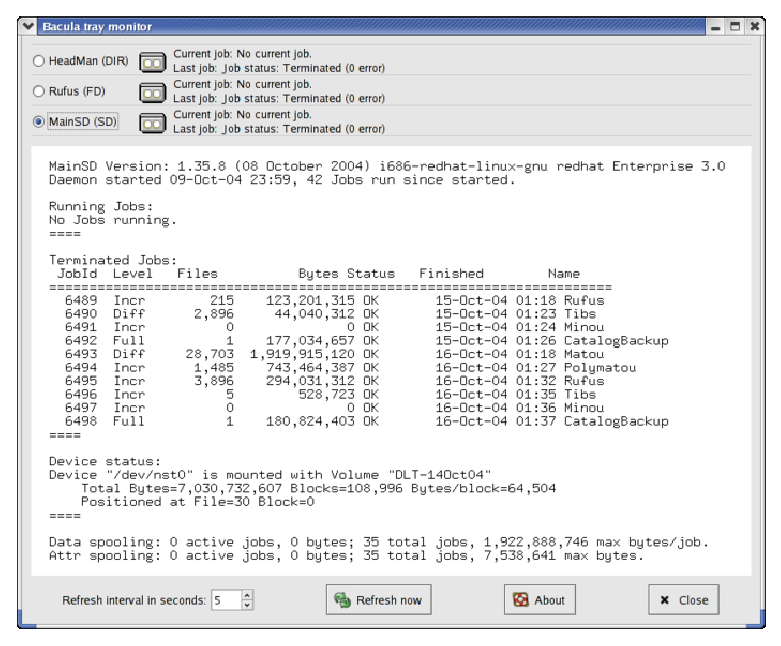
\includegraphics{./Bacula-tray-monitor.eps} 

The image shows a tray-monitor configured for three daemons. By clicking on
the radio buttons in the upper left corner of the image, you can see the
status for each of the daemons. The image shows the status for the Storage
daemon (MainSD) that is currently selected. 

The Monitor configuration file is found in the directory specified on the {\bf
\verb{--{sysconfdir} option that you specified on the {\bf ./configure} command and
by default is named {\bf tray-monitor.conf}. Normally, for first time users,
you just need to change the permission of this file to allow non-root users to
run the Monitor, as this application must run as the same user as the
graphical environment (don't forget allow non-root users to execute {\bf
bacula-tray-monitor}). This is not a security problem as long as you use the
default settings. 

\subsubsection*{
\ilink{Configuring the File daemon}{_ChapterStart25}}
\index[general]{Daemon!Configuring the File }
\index[general]{Configuring the File daemon }
\addcontentsline{toc}{subsubsection}{Configuring the File daemon}

The File daemon is a program that runs on each (Client) machine. At the
request of the Director, finds the files to be backed up and sends them (their
data) to the Storage daemon. 

The File daemon configuration file is found in the directory specified on the
{\bf \verb{--{sysconfdir} option that you specified on the {\bf ./configure} command.
By default, the File daemon's configuration file is named {\bf
bacula-fd.conf}. Normally, for first time users, no change is needed to this
file. Reasonable defaults are set. However, if you are going to back up more
than one machine, you will need to install the File daemon with a unique
configuration file on each machine to be backed up. The information about each
File daemon must appear in the Director's configuration file. 

\subsubsection*{
\ilink{Configuring the Director}{_ChapterStart40}}
\index[general]{Director!Configuring the }
\index[general]{Configuring the Director }
\addcontentsline{toc}{subsubsection}{Configuring the Director}

The Director is the central control program for all the other daemons. It
schedules and monitors all jobs to be backed up. 

The Director configuration file is found in the directory specified on the
{\bf \verb{--{sysconfdir} option that you specified on the {\bf ./configure} command.
Normally the Director's configuration file is named {\bf bacula-dir.conf}. 

In general, the only change you must make is modify the FileSet resource so
that the {\bf Include} configuration directive contains at least one line with
a valid name of a directory (or file) to be saved. 

If you do not have a DLT tape drive, you will probably want to edit the
Storage resource to contain names that are more representative of your actual
storage device. You can always use the existing names as you are free to
arbitrarily assign them, but they must agree with the corresponding names in
the Storage daemon's configuration file. 

You may also want to change the email address for notification from the
default {\bf root} to your email address. 

Finally, if you have multiple systems to be backed up, you will need a
separate File daemon or Client specification for each system, specifying its
name, address, and password. We have found that giving your daemons the same
name as your system but post fixed with {\bf -fd} helps a lot in debugging.
That is, if your system name is {\bf foobaz}, you would give the File daemon
the name {\bf foobaz-fd}. For the Director, you might use {\bf foobaz-dir},
and for the storage daemon, you might use {\bf foobaz-sd}. 

\subsubsection*{
\ilink{Configuring the Storage daemon}{_ChapterStart31}}
\index[general]{Daemon!Configuring the Storage }
\index[general]{Configuring the Storage daemon }
\addcontentsline{toc}{subsubsection}{Configuring the Storage daemon}

The Storage daemon is responsible, at the Director's request, for accepting
data from a File daemon and placing it on Storage media, or in the case of a
restore request, to find the data and send it to the File daemon. 

The Storage daemon's configuration file is found in the directory specified on
the {\bf \verb{--{sysconfdir} option that you specified on the {\bf ./configure}
command. By default, the Storage daemon's file is named {\bf bacula-sd.conf}.
Edit this file to contain the correct Archive device names for any tape
devices that you have. If the configuration process properly detected your
system, they will already be correctly set. These Storage resource name and
Media Type must be the same as the corresponding ones in the Director's
configuration file {\bf bacula-dir.conf}. If you want to backup to a file
instead of a tape, the Archive device must point to a directory in which the
Volumes will be created as files when you label the Volume. 
\label{ConfigTesting}

\subsection*{Testing your Configuration Files}
\index[general]{Testing your Configuration Files }
\index[general]{Files!Testing your Configuration }
\addcontentsline{toc}{subsection}{Testing your Configuration Files}

You can test if your configuration file is syntactically correct by running
the appropriate daemon with the {\bf -t} option. The daemon will process the
configuration file and print any error messages then terminate. For example,
assuming you have installed your binaries and configuration files in the same
directory. 

\footnotesize
\begin{verbatim}
cd <installation-directory>
./bacula-dir -t -c bacula-dir.conf
./bacula-fd -t -c bacula-fd.conf
./bacula-sd -t -c bacula-sd.conf
./bconsole -t -c bconsole.conf
./gnome-console -t -c gnome-console.conf
./wx-console -t -c wx-console.conf
su <normal user> -c "./bacula-tray-monitor -t -c tray-monitor.conf"
\end{verbatim}
\normalsize

will test the configuration files of each of the main programs. If the
configuration file is OK, the program will terminate without printing
anything. Please note that, depending on the configure options you choose,
some, or even all, of the three last commands will not be available on your
system. If you have installed the binaries in traditional Unix locations
rather than a single file, you will need to modify the above commands
appropriately (no ./ in front of the command name, and a path in front of the
conf file name). 
\label{TapeTesting}

\subsection*{Testing Bacula Compatibility with Your Tape Drive}
\index[general]{Drive!Testing Bacula Compatibility with Your Tape }
\index[general]{Testing Bacula Compatibility with Your Tape Drive }
\addcontentsline{toc}{subsection}{Testing Bacula Compatibility with Your Tape
Drive}

Before spending a lot of time on Bacula only to find that it doesn't work with
your tape drive, please read the 
\ilink{btape -- Testing Your Tape Drive}{_ChapterStart27}
chapter of this manual. If you have a modern standard SCSI tape drive on a
Linux or Solaris, most likely it will work, but better test than be sorry. For
FreeBSD (and probably other xBSD flavors), reading the above mentioned tape
testing chapter is a must. Also, for FreeBSD, please see 
\elink{The FreeBSD Diary}{http://www.freebsddiary.org/bacula.php} for a
detailed description on how to make Bacula work on your system. In addition,
users of FreeBSD prior to 4.9-STABLE dated Mon Dec 29 15:18:01 2003 UTC who
plan to use tape devices, please see the file {\bf
platforms/freebsd/pthreads-fix.txt} in the main Bacula directory concerning
important information concerning compatibility of Bacula and your system. 
\label{notls}

\subsection*{Get Rid of the /lib/tls Directory}
\index[general]{Directory!Get Rid of the /lib/tls }
\index[general]{Get Rid of the /lib/tls Directory }
\addcontentsline{toc}{subsection}{Get Rid of the /lib/tls Directory}

The new pthreads library {\bf /lib/tls} installed by default on recent Red Hat
systems running kernel 2.4.x is defective. You must remove it or rename it
then reboot your system before running Bacula otherwise after a week or so of
running, Bacula will either block for long periods or deadlock entirely. The
feedback that we have concerning 2.6 kernels is the same. However, on 2.6
systems, you may want to use the loader environment variable override rather
than removing /lib/tls. Please see 
\ilink{ Supported Operating Systems}{SupportedOSes} for more
information on this problem. 
\label{Running1}

\subsection*{Running Bacula}
\index[general]{Bacula!Running }
\index[general]{Running Bacula }
\addcontentsline{toc}{subsection}{Running Bacula}

Probably the most important part of running Bacula is being able to restore
files. If you haven't tried recovering files at least once, when you actually
have to do it, you will be under a lot more pressure, and prone to make
errors, than if you had already tried it once. 

To get a good idea how to use Bacula in a short time, we {\bf strongly}
recommend that you follow the example in the 
\ilink{Running Bacula Chapter}{_ChapterStart1} of this manual where
you will get detailed instructions on how to run Bacula. 

\subsection*{Log Rotation}
\index[general]{Rotation!Log }
\index[general]{Log Rotation }
\addcontentsline{toc}{subsection}{Log Rotation}

If you use the default {\bf bacula-dir.conf} or some variation of it, you will
note that it logs all the Bacula output to a file. To avoid that this file
grows without limit, we recommend that you copy the file {\bf logrotate} from
the {\bf scripts/logrotate} to {\bf /etc/logrotate.d/bacula}. This will cause
the log file to be rotated once a month and kept for a maximum of 5 months.
You may want to edit this file to change the default log rotation preferences.


\subsection*{Disaster Recovery}
\index[general]{Recovery!Disaster }
\index[general]{Disaster Recovery }
\addcontentsline{toc}{subsection}{Disaster Recovery}

If you intend to use Bacula as a disaster recovery tool rather than simply a
program to restore lost or damaged files, you will want to read the 
\ilink{Disaster Recovery Using Bacula Chapter}{_ChapterStart38} of
this manual. 

In any case, you are strongly urged to carefully test restoring some files
that you have saved rather than wait until disaster strikes. This way, you
will be prepared. 

%%
%%

\section*{Installing Bacula}
\label{_ChapterStart17}
\index[general]{Bacula!Installing }
\index[general]{Installing Bacula }
\addcontentsline{toc}{section}{Installing Bacula}

\subsection*{General}
\index[general]{General }
\addcontentsline{toc}{subsection}{General}

In general, you will need the Bacula source release, and if you want to run a
Windows client, you will need the Bacula Windows binary release. However,
Bacula needs certain third party packages (such as {\bf SQLite}, {\bf MySQL}
to build properly depending on the options you specify. To simplify your task,
we have combined a number of these packages into two {\bf depkgs} releases
(Dependency Packages). This can vastly simplify your life by providing you
with all the necessary packages rather than requiring you to find them on the
Web, load them, and install them. 
\label{upgrading1}

\subsection*{Upgrading Bacula}
\index[general]{Bacula!Upgrading }
\index[general]{Upgrading Bacula }
\addcontentsline{toc}{subsection}{Upgrading Bacula}

If you are upgrading from one Bacula version to another, you should first
carefully read the ReleaseNotes of all versions between your current version
and the version to which you are upgrading. If the Bacula catalog database has
been upgraded, you will either need to reinitialize your database starting
from scratch, or save an ASCII copy of your database, then proceed to upgrade
it. If there are several database upgrades between your version and the
version to which you are upgradding, you will need to apply each database
upgrade script. For your convenience, you can find all the old upgrade scripts
in the {\bf upgradedb} directory of the source code. You will need to edit the
scripts to correspond to your system configuration. The final upgrade script,
if any, will be in the {\bf src/cats} directory as described in the
ReleaseNotes. 

If you are upgrading from one major version to another, you will need to
replace all your components at the same time as generally the inter-daemon
protocol will change. However, within any particular release (e.g. version
1.32.x) unless there is an oversight or bug, the daemon protocol will not
change. If this is confusing, simply read the ReleaseNotes very carefully as
they will note if all daemons must be upgraded at the same time. 

Finally, please note that in general it is not necessary to do a 
{\bf make uninstall} before doing an upgrade. In fact, if you do so, you will 
most likely delete all your conf files, which could be disasterous.
For additional information on upgrading, please see the \ilink{Upgrading Bacula
Versions}{upgrading} in the Tips chapter of this manual.


\subsection*{Dependency Packages}
\label{Dependency}
\index[general]{Dependency Packages }
\index[general]{Packages!Dependency }
\addcontentsline{toc}{subsection}{Dependency Packages}

As discussed above, we have combined a number of third party packages that
Bacula might need into the {\bf depkgs} and {\bf depkgs1} releases. You can,
of course, get the latest packages from the original authors. The locations of
where we obtained the packages are in the README file in each package.
However, be aware that the packages in the depkgs files have been tested by us
for compatibility with Bacula. 

Typically, a dependency package will be named {\bf depkgs-ddMMMyy.tar.gz} and
{\bf depkgs1-ddMMyy.tar.gz} where {\bf dd} is the day we release it, {\bf MMM}
is the abbreviated month (e.g. Jan), and {\bf yy} is the year. An actual
example is: {\bf depkgs-07Apr02.tar.gz}. To install and build this package (if
needed), you do the following: 

\begin{enumerate}
\item Create a {\bf bacula} directory, into which you will place  both the
   Bacula source as well as the dependency package.  
\item Detar the {\bf depkg} into the {\bf bacula} directory.  
\item cd bacula/depkgs  
\item make 
   \end{enumerate}

Although the exact composition of the dependency packages may change from time
to time, the current makeup is the following: 

\addcontentsline{lot}{table}{Depedency Packages}
\begin{longtable}{|l|l|l|l|}
 \hline 
\multicolumn{1}{|c| }{\bf 3rd Party Package } & \multicolumn{1}{c| }{\bf
depkgs } & \multicolumn{1}{c| }{\bf depkgs1 } & \multicolumn{1}{c| }{\bf
depkgs-win32  } \\
 \hline {SQLite } & \multicolumn{1}{c| }{X } & \multicolumn{1}{c| }{- } &
\multicolumn{1}{c| }{-  } \\
 \hline {mtx } & \multicolumn{1}{c| }{X } & \multicolumn{1}{c| }{- } &
\multicolumn{1}{c| }{-  } \\
 \hline {readline } & \multicolumn{1}{c| }{- } & \multicolumn{1}{c| }{X } &
\multicolumn{1}{c| }{-  } \\
 \hline {pthreads } & \multicolumn{1}{c| }{- } & \multicolumn{1}{c| }{- } &
\multicolumn{1}{c| }{X  } \\
 \hline {zlib } & \multicolumn{1}{c| }{- } & \multicolumn{1}{c| }{- } &
\multicolumn{1}{c| }{X  } \\
 \hline {wxWidgits } & \multicolumn{1}{c| }{- } & \multicolumn{1}{c| }{- } &
\multicolumn{1}{c| }{X }
\\ \hline 

\end{longtable}

Note, some of these packages are quite large, so that building them can be a
bit time consuming. The above instructions will build all the packages
contained in the directory. However, when building Bacula, it will take only
those pieces that it actually needs. 

Alternatively, you can make just the packages that are needed. For example, 

\footnotesize
\begin{verbatim}
cd bacula/depkgs
make sqlite
\end{verbatim}
\normalsize

will configure and build only the SQLite package. 

You should build the packages that you will require in {\bf depkgs} and/or
{\bf depkgs1} prior to configuring and building Bacula, since Bacula will need
them during the build process. 

Even if you do not use SQLite, you might find it worthwhile to build {\bf mtx}
because the {\bf tapeinfo} program that comes with it can often provide you
with valuable information about your SCSI tape drive (e.g. compression,
min/max block sizes, ...). 

The {\bf depkgs-win32} package contains the source code for the pthreads and
zlib libraries used by the native Win32 client program. It will only be needed
if you intend to build the Win32 client from source. 

\subsection*{Supported Operating Systems}
\label{Systems}
\index[general]{Systems!Supported Operating }
\index[general]{Supported Operating Systems }
\addcontentsline{toc}{subsection}{Supported Operating Systems}

Please see the 
\ilink{ Supported Operating Systems}{SupportedOSes} section
of the QuickStart chapter of this manual. 

\subsection*{Building Bacula from Source}
\label{Building}
\index[general]{Source!Building Bacula from }
\index[general]{Building Bacula from Source }
\addcontentsline{toc}{subsection}{Building Bacula from Source}

The basic installation is rather simple. 

\begin{enumerate}
\item Install and build any {\bf depkgs} as noted above.  
\item Configure and install MySQL or PostgreSQL (if desired). 
   \ilink{Installing and Configuring MySQL Phase I}{_ChapterStart} or  
   \ilink{Installing and Configuring PostgreSQL Phase
   I}{_ChapterStart10}.  If you are installing from rpms, and are
   using MySQL, please be sure to install  {\bf mysql-devel}, so that the MySQL
   header files are available  while compiling Bacula. In addition, the MySQL
   client  library {\bf mysqlclient} requires the gzip compression library  {\bf
   libz.a} or {\bf libz.so}. If you are using rpm packages,  these libraries are
   in the {\bf libz-devel} package. On Debian  systems, you will need to load the
   {\bf zlib1g-dev} package. If  you are not using rpms or debs, you will need to
   find the  appropriate package for your system.  
   Note, if you already have a running MySQL or PostgreSQL on your system, you 
   can skip this phase provided that you have built the thread  safe libraries.
   And you have already installed the additional  rpms noted above.  
\item As an alternative to MySQL and PostgreSQL, configure and install SQLite,
    which is part of the {\bf depkgs}.  
   \ilink{Installing and Configuring SQLite}{_ChapterStart33}.  
   \item Detar the Bacula source code preferably into the {\bf bacula}  directory
   discussed above.  
\item {\bf cd} to the directory containing the source code.  
\item ./configure (with appropriate options as described below)  
\item Check the output of ./configure very carefully, especially  the Install
   binaries and Install config files directories.  If they are not correct,
   please rerun ./configure until they  are. The output from ./configure is
   stored in {\bf config.out}  and can be re-displayed at any time without
   rerunning the  ./configure by doing {\bf cat config.out}.  
\item If after running ./configure once, you decide to change options  and
   re-run it, that is perfectly fine, but before re-running it,  you should run: 


\footnotesize
\begin{verbatim}
      make distclean
      
\end{verbatim}
\normalsize

so that you are sure to start from scratch and not have a  mixture of the two
options. This is because ./configure  caches much of the information. The {\bf
make distclean}  is also critical if you move the source file from one 
machine to another. If the {\bf make distclean} fails,  just ignore it and
continue on.  
\item make  

   If you get errors while linking in the Storage daemon  directory (src/stored),
it is probably because you have not  loaded the static libraries on your
system. I noticed this  problem on a Solaris system. To correct it, make sure
that you  have not added {\bf \verb{--{enable-static-tools} to the  {\bf ./configure}
command. 
\item make install  
\item If you are new to Bacula, we {\bf strongly} recommend that you  skip the
   next step and use the default configuration files,  then run the example
   program in the next chapter, then  come back and modify your configuration
files to suit your  particular needs.  
\item Customize the configuration files for each of the three daemons 
   (Directory, File, Storage) and for the Console program. For the  details of
   how to do this, please see 
\ilink{Setting Up Bacula Configuration Files}{_ChapterStart16} in
the Configuration chapter of this manual.  We recommend that you start by
modifying the default configuration  files supplied, making the minimum
changes necessary.  Complete customization can be done after you have Bacula 
up and running.  Please take care when modifying passwords, which  were
randomly generated, and the {\bf Name}s as the  passwords and names must agree
between the configuration files  for security reasons. 
\item Create the Bacula MySQL database and tables (if using MySQL)  
   \ilink{Installing and Configuring MySQL Phase II}{mysql_phase2} or 
   create the Bacula PostgreSQL database and tables  
\ilink{Installing and Configuring PostgreSQL Phase
II}{PostgreSQL_phase2} or alternatively  if you are using
SQLite  
\ilink{Installing and Configuring SQLite Phase II}{phase2}.  
\item Start Bacula ({\bf ./bacula start}) Note. the next chapter  shows you
   how to do this in detail.  
\item Interface with Bacula using the Console program  
\item For the previous two items, please follow the instructions  in the 
   \ilink{Running Bacula}{_ChapterStart1} chapter of  this manual,
   where you will run a simple backup and do a  restore. Do this before you make
heavy modifications to the  configuration files so that you are sure that
Bacula works  and are familiar with it. After that changing the conf files 
will be easier.  
\item If after installing Bacula, you decide to ``move it'', that is  to
   install it in a different set of directories, proceed  as follows:  

\footnotesize
\begin{verbatim}
      make uninstall
      make distclean
      ./configure (your-new-options)
      make
      make install
      
\end{verbatim}
\normalsize

\end{enumerate}

If all goes well, the {\bf ./configure} will correctly determine which
operating system you are running and configure the source code appropriately.
Currently, FreeBSD, Linux (RedHat), and Solaris are supported. MacOS X 10.3 is
reported to work with the Client only as long as readline support is disabled.


If you install Bacula on more than one system, and they are identical, you can
simply transfer the source tree to that other system and do a ``make
install''. However, if there are differences in the libraries or OS versions,
or you wish to install on a different OS, you should start from the original
compress tar file. If you do transfer the source tree, and you have previously
done a ./configure command, you MUST do: 

\footnotesize
\begin{verbatim}
make distclean
\end{verbatim}
\normalsize

prior to doing your new ./configure. This is because the GNU autoconf tools
cache the configuration, and if you re-use a configuration for a Linux machine
on a Solaris, you can be sure your build will fail. To avoid this, as
mentioned above, either start from the tar file, or do a ``make distclean''. 

In general, you will probably want to supply a more complicated {\bf
configure} statement to ensure that the modules you want are built and that
everything is placed into the correct directories. 

For example, on RedHat, one could use the following: 

\footnotesize
\begin{verbatim}
CFLAGS="-g -Wall" \
  ./configure \
    --sbindir=$HOME/bacula/bin \
    --sysconfdir=$HOME/bacula/bin \
    --with-pid-dir=$HOME/bacula/bin/working \
    --with-subsys-dir=$HOME/bacula/bin/working \
    --with-mysql=$HOME/mysql \
    --with-working-dir=$HOME/bacula/bin/working \
    --with-dump-email=$USER
\end{verbatim}
\normalsize

Note, the advantage of using the above configuration to start is that
everything will be put into a single directory, which you can later delete
once you have run the examples in the next chapter and learned how Bacula
works. In addition, the above can be installed and run as non-root. 

For the developer's convenience, I have added a {\bf defaultconfig} script to
the {\bf examples} directory. This script contains the statements that you
would normally use, and each developer/user may modify them to suit his needs.
You should find additional useful examples in this directory as well. 

The {\bf \verb{--{enable-conio} or {\bf \verb{--{enable-readline} options are useful because
they provide a command line history and editing capability for the Console
program. If you have included either option in the build, either the {\bf
termcap} or the {\bf ncurses} package will be needed to link. On some systems,
such as SuSE, the termcap library is not in the standard library directory. As
a consequence, the option may be disabled or you may get an error message such
as: 

\footnotesize
\begin{verbatim}
/usr/lib/gcc-lib/i586-suse-linux/3.3.1/.../ld:
cannot find -ltermcap
collect2: ld returned 1 exit status
\end{verbatim}
\normalsize

while building the Bacula Console. In that case, you will need to set the {\bf
LDFLAGS} environment variable prior to building. 

\footnotesize
\begin{verbatim}
export LDFLAGS="-L/usr/lib/termcap"
\end{verbatim}
\normalsize

The same library requirements apply if you wish to use the readline
subroutines for command line editing and history or
 if you are using a MySQL library that requires encryption. If you need encryption,
you can either export the appropriate additional library options as shown
above or, alternatively, you can include them directly on the ./configure line
as in: 

\footnotesize
\begin{verbatim}
LDFLAGS="-lssl -lcyrpto" \
   ./configure \
      <your-options>
\end{verbatim}
\normalsize

On some systems such as Mandrake, readline tends to
gobble up prompts, which makes it totally useless. If this happens to you, use
the disable option, or if you are using version 1.33 and above try using {\bf
\verb{--{enable-conio} to use a built-in readline replacement. You will still need
the either termcap or ncurses library, but it is unlikely that the {\bf conio}
package will gobble up prompts. 

readline is no longer supported after version 1.34. The code is still
available and if users submit patches for it, I will be happy to apply them.
However, due to the fact that each version of readline seems to be
incompatible with previous versions, and that there are significant
differences between systems, I can no longer afford to support it. 

\subsection*{What Database to Use?}
\label{DB}
\index[general]{What Database to Use? }
\index[general]{Use!What Database to }
\addcontentsline{toc}{subsection}{What Database to Use?}

Before building Bacula you need to decide if you want to use SQLite, MySQL, or
PostgreSQL. If you are not already running MySQL or PostgreSQL, we recommend
that you start by using SQLite. This will greatly simplify the setup for you
because SQLite is compiled into Bacula an requires no administration. It
performs well and is suitable for small to medium sized installations (maximum
10-20 machines). 

If you wish to use MySQL as the Bacula catalog, please see the 
\ilink{Installing and Configuring MySQL}{_ChapterStart} chapter of
this manual. You will need to install MySQL prior to continuing with the
configuration of Bacula. MySQL is a high quality database that is very
efficient and is suitable for any sized installation. It is slightly more
complicated than SQLite to setup and administer because it has a number of
sophisticated features such as userids and passwords. It runs as a separate
process, is truly professional and can manage a database of any size. 

If you wish to use PostgreSQL as the Bacula catalog, please see the 
\ilink{Installing and Configuring PostgreSQL}{_ChapterStart10}
chapter of this manual. You will need to install PostgreSQL prior to
continuing with the configuration of Bacula. PostgreSQL is very similar to
MySQL, though it tends to be slightly more SQL92 compliant and has many more
advanced features such as transactions, stored procedures, and the such. It
requires a certain knowledge to install and maintain. There are some important
performance problems with PostgreSQL in Bacula versions prior to 1.35.5. 

If you wish to use SQLite as the Bacula catalog, please see 
\ilink{Installing and Configuring SQLite}{_ChapterStart33} chapter of
this manual. 

\subsection*{Quick Start}
\index[general]{Quick Start }
\index[general]{Start!Quick }
\addcontentsline{toc}{subsection}{Quick Start}

There are a number of options and important considerations given below
that you can skip for the moment if you have not had any problems building
Bacula with a simplified configuration as shown above. 

If you want to dive right into it, we recommend you skip to the next chapter,
and run the example program. It will teach you a lot about Bacula and as an
example can be installed into a single directory (for easy removal) and run as
non-root. If you have any problems or when you want to do a real installation,
come back to this chapter and read the details presented below. 

\subsection*{Configure Options}
\label{Options}
\index[general]{Options!Configure }
\index[general]{Configure Options }
\addcontentsline{toc}{subsection}{Configure Options}

The following command line options are available for {\bf configure} to
customize your installation. 

\begin{description}

\item [ \verb{--{sysbindir=\lt{}binary-path\gt{}]
   \index[dir]{\verb{--{sysbindir }
   Defines where the Bacula  binary (executable) files will be placed during a
   {\bf make  install} command.  

\item [ \verb{--{sysconfdir=\lt{}config-path\gt{}]
   \index[dir]{\verb{--{sysconfdir }
   Defines where the  Bacula configuration files should be placed during a {\bf
   make  install} command.  

\item [ \verb{--{enable-smartalloc ]
   \index[dir]{\verb{--{enable-smartalloc }
   This enables the inclusion of the  Smartalloc orphaned buffer detection code.
   This option is highly  recommended. Because we never build without this
   option, you may  experience problems if it is not enabled. In this case,
   simply  re-enable the option. We strongly recommend keeping this option 
   enabled as it helps detect memory leaks. This configuration  parameter is used
   while building Bacula  

\item [ \verb{--{enable-gnome ]
   \index[dir]{\verb{--{enable-gnome }
   If you have GNOME installed on your  computer and you want to use the GNOME
   GUI Console interface  to Bacula, you must specify this option. Doing so  will
   build everything in the {\bf src/gnome-console} directory.  

\item [ \verb{--{enable-wx-console ]
   \index[console]{\verb{--{enable-wx-console }
   If you have wxWidgets installed on your  computer and you want to use the
   wxWidgets GUI Console interface  to Bacula, you must specify this option.
   Doing so  will build everything in the {\bf src/wx-console} directory. This 
   could also be useful to users who want a GUI Console and don't  want to
   install Gnome, as wxWidgets can work with GTK+, Motif or even X11  libraries. 


\item [ \verb{--{enable-tray-monitor ]
   \index[dir]{\verb{--{enable-tray-monitor }
   If you have GTK installed on your  computer, you run an graphical environment
   or a window manager compatible  with the FreeDesktop system tray standard
   (like KDE and GNOME)  and you want to use a GUI to monitor Bacula daemons, you
   must specify  this option. Doing so will build everything in the  {\bf
   src/tray-monitor} directory.  

\item [ \verb{--{enable-static-tools]
   \index[dir]{\verb{--{enable-static-tools }
   This option causes the linker  to link the Storage daemon utility tools ({\bf
   bls},  {\bf bextract}, and {\bf bscan}) statically. This permits using  them
   without having the shared libraries loaded. If you have  problems linking in
   the {\bf src/stored} directory, make sure  you have not enabled this option,
   or explicitly  disable static linking by adding {\bf \verb{--{disable-static-tools}. 


\item [ \verb{--{enable-static-fd]
   \index[fd]{\verb{--{enable-static-fd }
   This option causes the make process  to build a {\bf static-bacula-fd} in
   addition to the standard  File daemon. This static version will include
   statically linked  libraries and is required for the Bare Metal recovery. This
   option  is largely superseded by using {\bf make static-bacula-fd} from with 
   in the {\bf src/filed} directory. Also, the {\bf \verb{--{enable-client-only}  option
   described below is useful for just building a client so that  all the other
   parts of the program are not compiled.  

\item [ \verb{--{enable-static-sd]
   \index[sd]{\verb{--{enable-static-sd }
   This option causes the make process  to build a {\bf static-bacula-sd} in
   addition to the standard  Storage daemon. This static version will include
   statically linked  libraries and could be useful during a Bare Metal recovery.
 

\item [ \verb{--{enable-static-dir]
   \index[dir]{\verb{--{enable-static-dir }
   This option causes the make process  to build a {\bf static-bacula-dir} in
   addition to the standard  Director. This static version will include
   statically linked  libraries and could be useful during a Bare Metal recovery.


\item [ \verb{--{enable-static-cons]
   \index[dir]{\verb{--{enable-static-cons }
   This option causes the make process  to build a {\bf static-console} and a
   {\bf static-gnome-console}  in addition to the standard console.  This static
   version will include statically linked  libraries and could be useful during a
   Bare Metal recovery.  

\item [ \verb{--{enable-client-only]
   \index[console]{\verb{--{enable-client-only }
   This option causes the make process  to build only the File daemon and the
   libraries that it needs.  None of the other daemons, storage tools, nor the
   console will  be built. Likewise a {\bf make install} will then only install 
   the File daemon. To cause all daemons to be built, you will need  to do a
   configuration without this option. This option greatly  facilitates building a
   Client on a client only machine.  

\item [ \verb{--{enable-largefile]
   \index[console]{\verb{--{enable-largefile }
   This option (default) causes  Bacula to be built with 64 bit file address
   support if it  is available on your system. This permits Bacula to read and 
   write files greater than 2 GBytes in size. You may disable this  feature and
   revert to 32 bit file addresses by using  {\bf \verb{--{disable-largefile}.  

\item [ \verb{--{with-sqlite=\lt{}sqlite-path\gt{}]
   \index[fd]{\verb{--{with-sqlite }
   This enables use of  the SQLite database. The {\bf sqlite-path} is not
   normally  specified as Bacula looks for the necessary components in  a
   standard location ({\bf depkgs/sqlite}). See 
   \ilink{Installing and Configuring SQLite}{_ChapterStart33} chapter of
    this manual for more details.  

\item [ \verb{--{with-mysql=\lt{}mysql-path\gt{}]
   \index[fd]{\verb{--{with-mysql }
   This enables building of the Catalog services for Bacula. It  assumes that
   MySQL is running on your system, and expects  it to be installed in the {\bf
   mysql-path} that you  specify. If this option is not present, the build will 
   automatically include the internal Bacula database  code. We recommend that
   you use this option if possible.  If you do use this option, please proceed to
   installing  MySQL in the 
   \ilink{Installing and Configuring MySQL}{_ChapterStart} chapter
   before proceeding with the configuration.  

\item [ \verb{--{with-postgresql=\lt{}path\gt{}]
   \index[fd]{\verb{--{with-postgresql }
   This provides an explicit  path to the PostgreSQL libraries if Bacula cannot
   find it by  default.  

\item [ \verb{--{enable-conio]
   \index[fd]{\verb{--{enable-conio }
   Tells Bacula to enable building the  small, light weight readline replacement
   routine. It is generally  much easier to configure than readline, although,
   like readline,  it needs either the termcap or ncurses library.  

\item [ \verb{--{with-readline=\lt{}readline-path\gt{}]
   \index[fd]{\verb{--{with-readline }
   Tells Bacula  where {\bf readline} is installed. Normally, Bacula will  find
   readline if it is in a standard library. If it is not found  and no
   \verb{--{with-readline is specified, readline will be disabled.  This option affects
   the Bacula build. Readline provides  the Console program with a command line
   history and editing  capability and is no longer supports, so you are on your
   own  if you have problems. 

\item [ \verb{--{enable-readline]
   \index[fd]{\verb{--{enable-readline }
   Tells Bacula to enable readline support.  It is normally disabled due to the
   large number of configuration  problems and the fact that the package seems to
   change in incompatible  ways from version to version.  

\item [ \verb{--{with-tcp-wrappers=\lt{}path\gt{}]
   \index[fd]{\verb{--{with-tcp-wrappers }
   This specifies that you  want TCP wrappers (man hosts\_access(5)) compiled in.
   The path is optional since  Bacula will normally find the libraries in the
   standard locations.  This option affects the Bacula build.  In specifying your
   restrictions in the {\bf /etc/hosts.allow}  or {\bf /etc/hosts.deny} files, do
   not use the {\bf twist}  option (hosts\_options(5)) or the Bacula process will
   be terminated.  
   
   For more information on configuring and testing TCP wrappers, please  see the 
   \ilink{Configuring and Testing TCP Wrappers}{wrappers}  section
   in the Security Capter.  

\item [ \verb{--{with-working-dir=\lt{}working-directory-path\gt{} ]
   \index[dir]{\verb{--{with-working-dir }
   This option is mandatory and specifies a directory  into which Bacula may
   safely place files that  will remain between Bacula executions. For example, 
   if the internal database is used, Bacula will keep  those files in this
   directory.  This option is only used to modify the daemon  configuration
   files. You may also accomplish the same  thing by directly editing them later.
   The working directory  is not automatically created by the install process, so
   you  must ensure that it exists before using Bacula for the  first time. 

\item [ \verb{--{with-base-port=\lt{}port=number\gt{}]
   \index[dir]{\verb{--{with-base-port }
   In order to run,  Bacula needs three TCP/IP ports (one for the Bacula 
   Console, one for the Storage daemon, and one for the File daemon).  The {\bf
   \verb{--{with-baseport} option will automatically assign three  ports beginning at
   the base port address specified. You may  also change the port number in the
   resulting configuration  files. However, you need to take care that the
   numbers  correspond correctly in each of the three daemon configuration 
   files. The default base port is 9101, which assigns ports 9101  through 9103.
   These ports (9101, 9102, and 9103) have been  officially assigned to Bacula by
   IANA.  This option is only used  to modify the daemon configuration files. You
   may also accomplish  the same thing by directly editing them later. 

\item [ \verb{--{with-dump-email=\lt{}email-address\gt{}]
   \index[dir]{\verb{--{with-dump-email }
   This option specifies  the email address where any core dumps should be set.
   This option  is normally only used by developers.  

\item [ \verb{--{with-pid-dir=\lt{}PATH\gt{}  ]
   \index[dir]{\verb{--{with-pid-dir }
   This specifies where Bacula should place the process id  file during
   execution. The default is: {\bf /var/run}.  This directory is not created by
   the install process, so  you must ensure that it exists before using Bacula
   the  first time.  

\item [ \verb{--{with-subsys-dir=\lt{}PATH\gt{}]
   \index[dir]{\verb{--{with-subsys-dir }
   This specifies where Bacula should place the subsystem lock  file during
   execution. The default is {\bf /var/run/subsys}.  Please make sure that you do
   not specify the same directory  for this directory and for the {\bf sbindir}
   directory.  This directory is used only within the autostart scripts.  The
   subsys directory is not created by the Bacula install,  so you must be sure to
   create it before using Bacula. 

\item [ \verb{--{with-dir-password=\lt{}Password\gt{}]
   \index[dir]{\verb{--{with-dir-password }
   This option allows you to specify the password used to  access the Directory
   (normally from the Console program).  If it is not specified, configure will
   automatically create a random  password.  

\item [ \verb{--{with-fd-password=\lt{}Password\gt{} ]
   \index[fd]{\verb{--{with-fd-password }
   This option allows you to specify the password used to  access the File daemon
   (normally called from the Director).  If it is not specified, configure will
   automatically create a random  password.  

\item [ \verb{--{with-sd-password=\lt{}Password\gt{} ]
   \index[sd]{\verb{--{with-sd-password }
   This option allows you to specify the password used to  access the Directory
   (normally called from the Director).  If it is not specified, configure will
   automatically create a random  password.  

\item [ \verb{--{with-dir-user=\lt{}User\gt{} ]
   \index[dir]{\verb{--{with-dir-user }
   This option allows you to specify the Userid used to  run the Director. The
   Director must be started as root, but  doesn't need to run as root, and  after
   doing preliminary initializations, it can ``drop''  to the UserId specified on
   this option. 

\item [ \verb{--{with-dir-group=\lt{}Group\gt{} ]
   \index[dir]{\verb{--{with-dir-group }
   This option allows you to specify the GroupId used to  run the Director. The
   Director must be started as root, but  doesn't need to run as root, and  after
   doing preliminary initializations, it can ``drop''  to the GroupId specified
   on this option. 

\item [ \verb{--{with-sd-user=\lt{}User\gt{} ]
   \index[sd]{\verb{--{with-sd-user }
   This option allows you to specify the Userid used to  run the Storage daemon.
   The Storage daemon must be started as root, but  doesn't need to run as root,
   and  after doing preliminary initializations, it can ``drop''  to the UserId
   specified on this option. If you use this option,  you will need to take care
   that the Storage daemon has access  to all the devices (tape drives, ...) that
   it needs. 

\item [ \verb{--{with-sd-group=\lt{}Group\gt{} ]
   \index[sd]{\verb{--{with-sd-group }
   This option allows you to specify the GroupId used to  run the Storage daemon.
   The Storage daemon must be started as root, but  doesn't need to run as root,
   and  after doing preliminary initializations, it can ``drop''  to the GroupId
   specified on this option. 

\item [ \verb{--{with-fd-user=\lt{}User\gt{} ]
   \index[fd]{\verb{--{with-fd-user }
   This option allows you to specify the Userid used to  run the File daemon. The
   File daemon must be started as root,  and in most cases, it needs to run as
   root, so this option is  used only in very special cases,  after doing
   preliminary initializations, it can ``drop''  to the UserId specified on this
   option. 

\item [ \verb{--{with-fd-group=\lt{}Group\gt{} ]
   \index[fd]{\verb{--{with-fd-group }
   This option allows you to specify the GroupId used to  run the File daemon.
   The File daemon must be started as root, and  in most cases, it must be run as
   root, however,  after doing preliminary initializations, it can ``drop''  to
   the GroupId specified on this option. 

\end{description}

Note, many other options are presented when you do a {\bf ./configure \verb{--{help},
but they are not implemented. 

\subsection*{Recommended Options for most Systems}
\index[general]{Systems!Recommended Options for most }
\index[general]{Recommended Options for most Systems }
\addcontentsline{toc}{subsection}{Recommended Options for most Systems}

For most systems, we recommend starting with the following options: 

\footnotesize
\begin{verbatim}
./configure \
  --enable-smartalloc \
  --sbindir=$HOME/bacula/bin \
  --sysconfdir=$HOME/bacula/bin \
  --with-pid-dir=$HOME/bacula/bin/working \
  --with-subsys-dir=$HOME/bacula/bin/working \
  --with-mysql=$HOME/mysql \
  --with-working-dir=$HOME/bacula/working
\end{verbatim}
\normalsize

If you want to install Bacula in an installation directory rather than run it
out of the build directory (as developers will do most of the time), you
should also include the \verb{--{sbindir and \verb{--{sysconfdir options with appropriate
paths. Neither are necessary if you do not use ``make install'' as is the case
for most development work. The install process will create the sbindir and
sysconfdir if they do not exist, but it will not automatically create the
pid-dir, subsys-dir, or working-dir, so you must ensure that they exist before
running Bacula for the first time. See below for an example of how Kern does
it. 

\subsection*{RedHat}
\index[general]{RedHat }
\addcontentsline{toc}{subsection}{RedHat}

Using SQLite: 

\footnotesize
\begin{verbatim}
 
CFLAGS="-g -Wall" ./configure \
  --sbindir=$HOME/bacula/bin \
  --sysconfdir=$HOME/bacula/bin \
  --enable-smartalloc \
  --with-sqlite=$HOME/bacula/depkgs/sqlite \
  --with-working-dir=$HOME/bacula/working \
  --with-pid-dir=$HOME/bacula/bin/working \
  --with-subsys-dir=$HOME/bacula/bin/working \
  --enable-gnome \
  --enable-conio
\end{verbatim}
\normalsize

or 

\footnotesize
\begin{verbatim}
 
CFLAGS="-g -Wall" ./configure \
  --sbindir=$HOME/bacula/bin \
  --sysconfdir=$HOME/bacula/bin \
  --enable-smartalloc \
  --with-mysql=$HOME/mysql \
  --with-working-dir=$HOME/bacula/working
  --with-pid-dir=$HOME/bacula/bin/working \
  --with-subsys-dir=$HOME/bacula/bin/working
  --enable-gnome \
  --enable-conio
\end{verbatim}
\normalsize

or finally, a completely traditional RedHat Linux install: 

\footnotesize
\begin{verbatim}
CFLAGS="-g -Wall" ./configure \
  --prefix=/usr \
  --sbindir=/usr/sbin \
  --sysconfdir=/etc/bacula \
  --with-scriptdir=/etc/bacula \
  --enable-smartalloc \
  --enable-gnome \
  --with-mysql \
  --with-working-dir=/var/bacula \
  --with-pid-dir=/var/run \
  --with-subsys-dir=/var/lock/subsys \
  --enable-conio
\end{verbatim}
\normalsize

Note, Bacula assumes that /var/bacula, /var/run, and /var/loc/subsys exist so
it will not automatically create them during the install process. 

\subsection*{Solaris}
\index[general]{Solaris }
\addcontentsline{toc}{subsection}{Solaris}

To build Bacula from source, you will need the following installed on your
system (they are not by default): libiconv, gcc 3.3.2, stdc++, libgcc (for
stdc++ and gcc\_s libraries), make 3.8 or later. 

You will probably also need to: Add /usr/local/bin to PATH and Add
/usr/ccs/bin to PATH for ar. 

\footnotesize
\begin{verbatim}
#!/bin/sh
CFLAGS="-g" ./configure \
  --sbindir=$HOME/bacula/bin \
  --sysconfdir=$HOME/bacula/bin \
  --with-mysql=$HOME/mysql \
  --enable-smartalloc \
  --with-pid-dir=$HOME/bacula/bin/working \
  --with-subsys-dir=$HOME/bacula/bin/working \
  --with-working-dir=$HOME/bacula/working
\end{verbatim}
\normalsize

As mentioned above, the install process will create the sbindir and sysconfdir
if they do not exist, but it will not automatically create the pid-dir,
subsys-dir, or working-dir, so you must ensure that they exist before running
Bacula for the first 

\subsection*{FreeBSD}
\index[general]{FreeBSD }
\addcontentsline{toc}{subsection}{FreeBSD}

Please see: 
\elink{The FreeBSD Diary}{http://www.freebsddiary.org/bacula.php} for a
detailed description on how to make Bacula work on your system. In addition,
users of FreeBSD prior to 4.9-STABLE dated Mon Dec 29 15:18:01 2003 UTC who
plan to use tape devices, please see the 
\ilink{Tape Testing Chapter}{FreeBSDTapes} of this manual for
{\bf important} information on how to configure your tape drive for
compatibility with Bacula. 

If you are using Bacula with MySQL, you should take care to compile MySQL with
FreeBSD native threads rather than LinuxThreads, since Bacula is normal built
with FreeBSD native threads rather than LinuxTreads. Mixing the two will
probably not work. 

\subsection*{Win32}
\index[general]{Win32 }
\addcontentsline{toc}{subsection}{Win32}

To install the binary Win32 version of the File daemon please see the 
\ilink{Win32 Installation Chapter}{_ChapterStart7} in this document. 

\subsection*{Windows Systems with CYGWIN Installed}
\label{Win32}
\index[general]{Windows Systems with CYGWIN Installed }
\index[general]{Installed!Windows Systems with CYGWIN }
\addcontentsline{toc}{subsection}{Windows Systems with CYGWIN Installed}

As of version 1.34, Bacula no longer uses CYGWIN for the Win32 File daemon.
However, it is still built under a CYGWIN build environment -- though you can
probably do it with VC Studio only. If you wish to build the Win32 File daemon
from the source, you will need Microsoft C++ version 6.0 or greater. In Bacula
prior to version 1.33, CYGWIN was used. Details for building it are in the
README file of the src/win32 directory. 

Note, although most parts of Bacula build on Windows systems, the only part
that we have tested and used is the File daemon. 

Finally, you should follow the installation instructions in the 
\ilink{Win32 Installation}{_ChapterStart7} section of this document. 

\subsection*{Kern's Configure Script}
\index[general]{Script!Kern's Configure }
\index[general]{Kern's Configure Script }
\addcontentsline{toc}{subsection}{Kern's Configure Script}

The script that I use for building on my ``production'' Linux machines is: 

\footnotesize
\begin{verbatim}
#!/bin/sh
# This is Kern's configure script for Bacula
CFLAGS="-g -Wall" \
  ./configure \
    --sbindir=$HOME/bacula/bin \
    --sysconfdir=$HOME/bacula/bin \
    --enable-smartalloc \
    --enable-gnome \
    --with-pid-dir=$HOME/bacula/bin/working \
    --with-subsys-dir=$HOME/bacula/bin/working \
    --with-mysql=$HOME/mysql \
    --with-working-dir=$HOME/bacula/bin/working \
    --with-dump-email=$USER \
    --with-smtp-host=mail.your-site.com \
    --with-baseport=9101
exit 0
\end{verbatim}
\normalsize

Note that I define the base port as 9101, which means that Bacula will use
port 9101 for the Director console, port 9102 for the File daemons, and port
9103 for the Storage daemons. These ports should be available on all systems
because they have been officially assigned to Bacula by IANA (Internet
Assigned Numbers Authority). We strongly recommend that you use only these
ports to prevent any conflicts with other programs. This is in fact the
default if you do not specify a {\bf \verb{--{with-baseport} option. 

You may also want to put the following entries in your {\bf /etc/services}
file as it will make viewing the connections made by Bacula easier to
recognize (i.e. netstat -a): 

\footnotesize
\begin{verbatim}
bacula-dir      9101/tcp
bacula-fd       9102/tcp
bacula-sd       9103/tcp
\end{verbatim}
\normalsize

\subsection*{Installing Bacula}
\index[general]{Bacula!Installing }
\index[general]{Installing Bacula }
\addcontentsline{toc}{subsection}{Installing Bacula}

Before setting up your configuration files, you will want to install Bacula in
its final location. Simply enter: 

\footnotesize
\begin{verbatim}
make install
\end{verbatim}
\normalsize

If you have previously installed Bacula, the old binaries will be overwritten,
but the old configuration files will remain unchanged, and the ``new''
configuration files will be appended with a {\bf .new}. Generally if you have
previously installed and run Bacula you will want to discard or ignore the
configuration files with the appended {\bf .new}. 

\subsection*{Building a File Daemon or Client}
\index[general]{Client!Building a File Daemon or }
\index[general]{Building a File Daemon or Client }
\addcontentsline{toc}{subsection}{Building a File Daemon or Client}

If you run the Director and the Storage daemon on one machine and you wish to
back up another machine, you must have a copy of the File daemon for that
machine. If the machine and the Operating System are identical, you can simply
copy the Bacula File daemon binary file {\bf bacula-fd} as well as its
configuration file {\bf bacula-fd.conf} then modify the name and password in
the conf file to be unique. Be sure to make corresponding additions to the
Director's configuration file ({\bf bacula-dir.conf}). 

If the architecture or the O/S level are different, you will need to build a
File daemon on the Client machine. To do so, you can use the same {\bf
./configure} command as you did for your main program, starting either from a
fresh copy of the source tree, or using {\bf make\ distclean} before the {\bf
./configure}. 

Since the File daemon does not access the Catalog database, you can remove the
{\bf \verb{--{with-mysql} or {\bf \verb{--{with-sqlite} options, then add {\bf
\verb{--{enable-client-only}. This will compile only the necessary libraries and the
client programs and thus avoids the necessity of installing one or another of
those database programs to build the File daemon. With the above option, you
simply enter {\bf make} and just the client will be built. 
\label{autostart}

\subsection*{Auto Starting the Daemons}
\index[general]{Daemons!Auto Starting the }
\index[general]{Auto Starting the Daemons }
\addcontentsline{toc}{subsection}{Auto Starting the Daemons}

If you wish the daemons to be automatically started and stopped when your
system is booted (a good idea), one more step is necessary. First, the
./configure process must recognize your system -- that is it must be a
supported platform and not {\bf unknown}, then you must install the platform
dependent files by doing: 

\footnotesize
\begin{verbatim}
(become root)
make install-autostart
\end{verbatim}
\normalsize

Please note, that the auto-start feature is implemented only on systems that
we officially support (currently, FreeBSD, RedHat Linux, and Solaris), and has
only been fully tested on RedHat Linux. 

The {\bf make install-autostart} will cause the appropriate startup scripts to
be installed with the necessary symbolic links. On RedHat Linux systems, these
scripts reside in {\bf /etc/rc.d/init.d/bacula-dir} {\bf
/etc/rc.d/init.d/bacula-fd}, and {\bf /etc/rc.d/init.d/bacula-sd}. However the
exact location depends on what operating system you are using. 

If you only wish to install the File daemon, you may do so with: 

\footnotesize
\begin{verbatim}
make install-autostart-fd
\end{verbatim}
\normalsize

\subsection*{Other Make Notes}
\index[general]{Notes!Other Make }
\index[general]{Other Make Notes }
\addcontentsline{toc}{subsection}{Other Make Notes}

To simply build a new executable in any directory, enter: 

\footnotesize
\begin{verbatim}
make
\end{verbatim}
\normalsize

To clean out all the objects and binaries (including the files named 1, 2, or
3, which Kern uses as temporary files), enter: 

\footnotesize
\begin{verbatim}
make clean
\end{verbatim}
\normalsize

To really clean out everything for distribution, enter: 

\footnotesize
\begin{verbatim}
make distclean
\end{verbatim}
\normalsize

note, this cleans out the Makefiles and is normally done from the top level
directory to prepare for distribution of the source. To recover from this
state, you must redo the {\bf ./configure} in the top level directory, since
all the Makefiles will be deleted. 

To add a new file in a subdirectory, edit the Makefile.in in that directory,
then simply do a {\bf make}. In most cases, the make will rebuild the Makefile
from the new Makefile.in. In some case, you may need to issue the {\bf make} a
second time. In extreme cases, cd to the top level directory and enter: {\bf
make Makefiles}. 

To add dependencies: 

\footnotesize
\begin{verbatim}
make depend
\end{verbatim}
\normalsize

The {\bf make depend} appends the header file dependencies for each of the
object files to Makefile and Makefile.in. This command should be done in each
directory where you change the dependencies. Normally, it only needs to be run
when you add or delete source or header files. {\bf make depend} is normally
automatically invoked during the configuration process. 

To install: 

\footnotesize
\begin{verbatim}
make install
\end{verbatim}
\normalsize

This not normally done if you are developing Bacula, but is used if you are
going to run it to backup your system. 

After doing a {\bf make install} the following files will be installed on your
system (more or less). The exact files and location (directory) for each file
depends on your {\bf ./configure} command (e.g. gnome-console and
gnome-console.conf are not installed if you do not configure GNOME. Also, if
you are using SQLite instead of mysql, some of the files will be different). 

\footnotesize
\begin{verbatim}
bacula
bacula-dir
bacula-dir.conf
bacula-fd
bacula-fd.conf
bacula-sd
bacula-sd.conf
bacula-tray-monitor
tray-monitor.conf
bextract
bls
bscan
btape
btraceback
btraceback.gdb
bconsole
bconsole.conf
create_mysql_database
dbcheck
delete_catalog_backup
drop_bacula_tables
drop_mysql_tables
fd
gnome-console
gnome-console.conf
make_bacula_tables
make_catalog_backup
make_mysql_tables
mtx-changer
query.sql
bsmtp
startmysql
stopmysql
wx-console
wx-console.conf
\end{verbatim}
\normalsize

\label{monitor}

\subsection*{Installing Tray Monitor}
\index[general]{Monitor!Installing Tray }
\index[general]{Installing Tray Monitor }
\addcontentsline{toc}{subsection}{Installing Tray Monitor}

The Tray Monitor is already installed if you used the {\bf
\verb{--{enable-tray-monitor} configure option and ran {\bf make install}.

As you don't run your graphical environment as root (if you do, you should
change that bad habit), don't forget to allow your user to read {\bf
tray-monitor.conf}, and to execute {\bf bacula-tray-monitor} (this is not a
security issue).

Then log into your graphical environment (KDE, Gnome or something else), run
{\bf bacula-tray-monitor} as your user, and see if a cassette icon appear
somewhere on the screen, usually on the task bar.
If it doesn't, follow the instructions below related to your environment or
window manager. 

\subsubsection*{GNOME}
\index[general]{GNOME }
\addcontentsline{toc}{subsubsection}{GNOME}

System tray, or notification area if you use the GNOME terminology, has been
supported in GNOME since version 2.2. To activate it, right-click on one of
your panels, open the menu {\bf Add to this Panel}, then {\bf Utility} and
finally click on {\bf Notification Area}. 

\subsubsection*{KDE}
\index[general]{KDE }
\addcontentsline{toc}{subsubsection}{KDE}

System tray has been supported in KDE since version 3.1. To activate it,
right-click on one of your panels, open the menu {\bf Add}, then {\bf Applet}
and finally click on {\bf System Tray}. 

\subsubsection*{Other window managers}
\index[general]{Managers!Other window }
\index[general]{Other window managers }
\addcontentsline{toc}{subsubsection}{Other window managers}

Read the documentation to know if the Freedesktop system tray standard is
supported by your window manager, and if applicable, how to activate it. 

\subsection*{Modifying the Bacula Configuration Files}
\index[general]{Modifying the Bacula Configuration Files }
\index[general]{Files!Modifying the Bacula Configuration }
\addcontentsline{toc}{subsection}{Modifying the Bacula Configuration Files}

See the chapter 
\ilink{Configuring Bacula}{_ChapterStart16} in this manual for
instructions on how to set Bacula configuration files. 

%%
%%

\section*{Critical Items to Implement Before Going Production}
\label{_ChapterStart32}
\index[general]{Production!Critical Items to Implement Before Going }
\index[general]{Critical Items to Implement Before Going Production }
\addcontentsline{toc}{section}{Critical Items to Implement Before Going
Production}

\subsection*{General}
\index[general]{General }
\addcontentsline{toc}{subsection}{General}

We recommend you take your time before implementing a Bacula backup system
since Bacula is a rather complex program, and if you make a mistake, you may
suddenly find that you cannot restore the your files in case of a disaster.
This is especially true if you have not previously used a major backup
product. 

If you follow the instructions in this chapter, you will have covered most of
the major problems that can occur. It goes without saying that if ever you
find that we have left out an important point, please point it out to us, so
that we can document it to the benefit of everyone. 

\label{Critical}
\subsection*{Critical Items}
\index[general]{Critical Items }
\index[general]{Items!Critical }
\addcontentsline{toc}{subsection}{Critical Items}

The following assumes that you have installed Bacula, you more or less
understand it, you have at least worked through the tutorial or have
equivalent experience, and that you have setup a basic production
configuration. If you haven't done the above, please do so then come back
here. The following is a sort of checklist that points you elsewhere in the
manual with perhaps a brief explaination of why you should do it. The order is
more or less the order you would use in setting up a production system (if you
already are in production, use the checklist anyway). 

\begin{itemize}
\item Test your tape drive with compatibility with Bacula by using the  test
   command in the \ilink{btape}{btape} program. 
\item Better than doing the above is to walk through the nine steps in the  
   \ilink{Tape Testing}{_ChapterStart27} chapter of the manual. It 
   may take you a bit of time, but it will eliminate surprises. 
\item Make sure that /lib/tls is disabled. Bacula does not work with this 
   library. See the second point under 
   \ilink{ Supported Operating Systems.}{SupportedOSes} 
\item Do at least one restore of files. If you backup both Unix and Win32
   systems,  restore files from each system type. The 
   \ilink{Restoring Files}{_ChapterStart13} chapter shows you how. 
\item Write a bootstrap file to a separate system for each backup job.  The
   Write Bootstrap directive is described in the  
   \ilink{Director Configuration}{writebootstrap}  chapter of the
   manual, and more details are available in the  
   \ilink{Bootstrap File}{_ChapterStart43} chapter. Also, the default
   bacula-dir.conf comes with a Write Bootstrap directive defined. This  allows
   you to recover the state of your system as of the last backup.  
\item Backup your catalog. An example of this is found in the default 
   bacula-dir.conf file. The backup script is installed by default and  should
   handle any database, though you may want to make your own  local
   modifications.  
\item Write a bootstrap file for the catalog. An example of this is found in
   the default bacula-dir.conf file. This will allow you to quickly restore your
   catalog in the event it is wiped out -- otherwise it  is many excruciating
   hours of work.  
\item Make a Bacula Rescue CDROM! See the 
   \ilink{Disaster Recovery Using a Bacula Rescue
   CDROM}{_ChapterStart38} chapter. It is trivial to  make such a CDROM,
   and it can make system recovery in the event of  a lost hard disk infinitely
   easier. 
\end{itemize}

\subsection*{Recommended Items}
\index[general]{Items!Recommended }
\index[general]{Recommended Items }
\addcontentsline{toc}{subsection}{Recommended Items}

Although these items may not be critical, they are recommended and will help
you avoid problems. 

\begin{itemize}
\item Read the \ilink{Quick Start Guide to Bacula}{_ChapterStart37} 
\item After installing and experimenting with Bacula, read and work carefully 
   through the examples in the 
   \ilink{Tutorial}{_ChapterStart1} chapter  of this manual. 
\item Learn what each of the \ilink{Bacula Utility Programs}{_ChapterStart9}  does. 
\item Set up reasonable retention periods so that your catalog does not  grow
   to be too big. See the following three chapters:\\
   \ilink{Recycling your Volumes}{_ChapterStart22},\\
   \ilink{Basic Volume Management}{_ChapterStart39},\\
   \ilink{Using Pools to Manage Volumes}{_ChapterStart11}. 
\item Perform a bare metal recovery using the Bacula Rescue CDROM.  See the 
   \ilink{Disaster Recovery Using a Bacula Rescue CDROM}{_ChapterStart38} chapter. 
   \end{itemize}

%%
%%

\section*{A Brief Tutorial}
\label{_ChapterStart1}
\index[general]{Brief Tutorial }
\index[general]{Tutorial!Brief }
\addcontentsline{toc}{section}{Brief Tutorial}

This chapter will guide you through running Bacula. To do so, we assume you
have installed Bacula, possibly in a single file as shown in the previous
chapter, in which case, you can run Bacula as non-root for these tests.
However, we assume that you have not changed the .conf files. If you have
modified the .conf files, please go back and uninstall Bacula, then reinstall
it, but do not make any changes. The examples in this chapter use the default
configuration files, and will write the volumes to disk in your {\bf /tmp}
directory, in addition, the data backed up will be the source directory where
you built Bacula. As a consequence, you can run all the Bacula daemons for
these tests as non-root. Please note, in production, your File daemon(s) must
run as root. See the Security chapter for more information on this subject. 

The general flow of running Bacula is: 

\begin{enumerate}
\item cd \lt{}install-directory\gt{}  
\item Start the Database (if using MySQL or PostgreSQL)  
\item Start the Daemons with {\bf ./bacula start}  
\item Start the Console program to interact with the Director  
\item Run a job  
\item When the Volume fills, unmount the Volume, if it is a  tape, label a new
   one, and continue running. In this  chapter, we will write only to disk files
   so you won't  need to worry about tapes for the moment. 
\item Test recovering some files from the Volume just written to  ensure the
   backup is good and that you know how to recover.  Better test before disaster
   strikes  
\item Add a second client. 
   \end{enumerate}

Each of these steps is described in more detail below. 

\subsection*{Before Running Bacula}
\index[general]{Bacula!Before Running }
\index[general]{Before Running Bacula }
\addcontentsline{toc}{subsection}{Before Running Bacula}

Before running Bacula for the first time in production, we recommend that you
run the {\bf test} command in the {\bf btape} program as described in the 
\ilink{Utility Program Chapter}{btape} of this manual. This will
help ensure that Bacula functions correctly with your tape drive. If you have
a modern HP, Sony, or Quantum DDS or DLT tape drive running on Linux or
Solaris, you can probably skip this test as Bacula is well tested with these
drives and systems. For all other cases, you are {\bf strongly} encouraged to
run the test before continuing. {\bf btape} also has a {\bf fill} command that
attempts to duplicate what Bacula does when filling a tape and writing on the
next tape. You should consider trying this command as well, but be forewarned,
it can take hours (about 4 hours on my drive) to fill a large capacity tape. 

\subsection*{Starting the Database}
\label{StartDB}
\index[general]{Starting the Database }
\index[general]{Database!Starting the }
\addcontentsline{toc}{subsection}{Starting the Database}

If you are using MySQL or PostgreSQL as the Bacula database, you should start
it before you attempt to run a job to avoid getting error messages from Bacula
when it starts. The scripts {\bf startmysql} and {\bf stopmysql} are what I
(Kern) use to start and stop my local MySQL. Note, if you are using SQLite,
you will not want to use {\bf startmysql} or {\bf stopmysql}. If you are
running this in production, you will probably want to find some way to
automatically start MySQL or PostgreSQL after each system reboot. 

If you are using SQLite (i.e. you specified the {\bf \verb{--{with-sqlite=xxx} option
on the {\bf ./configure} command, you need do nothing. SQLite is automatically
started by {\bf Bacula}. 

\subsection*{Starting the Daemons}
\label{StartDaemon}
\index[general]{Starting the Daemons }
\index[general]{Daemons!Starting the }
\addcontentsline{toc}{subsection}{Starting the Daemons}

To start the three daemons, from your installation directory, simply enter: 

./bacula start This script starts the Storage daemon, the File daemon, and the
Director daemon, which all normally run as daemons in the background. If you
are using the autostart feature of Bacula, your daemons will either be
automatically started on reboot, or you can control them individually with the
files {\bf bacula-dir}, {\bf bacula-fd}, and {\bf bacula-sd}, which are
usually located in {\bf /etc/init.d}, though the actual location is system
dependent. 

Note, on Windows, currently only the File daemon is ported, and it must be
started differently. Please see the 
\ilink{Windows Version of Bacula}{_ChapterStart7} Chapter of this
manual. 

The rpm packages configure the daemons to run as user=root and group=bacula.
The rpm installation also creates the group bacula if it does not exist on the
system. Any users that you add to the group bacula will have access to files
created by the daemons. To disable or alter this behavior edit the daemon
startup scripts: 

\begin{itemize}
\item /etc/bacula/bacula 
\item /etc/init.d/bacula-dir 
\item /etc/init.d/bacula-sd 
\item /etc/init.d/bacula-fd 
   \end{itemize}

and then restart as noted above. 

The 
\ilink{installation chapter}{_ChapterStart17} of this manual
explains how you can install scripts that will automatically restart the
daemons when the system starts. 

\subsection*{Interacting with the Director to Query or Start Jobs}
\index[general]{Jobs!Interacting with the Director to Query or Start }
\index[general]{Interacting with the Director to Query or Start Jobs }
\addcontentsline{toc}{subsection}{Interacting with the Director to Query or
Start Jobs}

To communicate with the director and to query the state of Bacula or run jobs,
from the top level directory, simply enter: 

./bconsole 

Note, on 1.32 versions and lower, the command name is {\bf console} rather
than bconsole. Alternatively to running the command line console, if you have
GNOME installed and used the {\bf \verb{--{enable-gnome} on the configure command,
you may use the GNOME Console program: 

./gnome-console 

For simplicity, here we will describe only the {\bf ./console} program. Most
of what is described here applies equally well to {\bf ./gnome-console}. 

The {\bf ./bconsole} runs the Bacula Console program, which connects to the
Director daemon. Since Bacula is a network program, you can run the Console
program anywhere on your network. Most frequently, however, one runs it on the
same machine as the Director. Normally, the Console program will print
something similar to the following: 

\footnotesize
\begin{verbatim}
[kern@polymatou bin]$ ./bconsole
Connecting to Director lpmatou:9101
1000 OK: HeadMan Version: 1.30 (28 April 2003)
*
\end{verbatim}
\normalsize

the asterisk is the console command prompt. 

Type {\bf help} to see a list of available commands: 

\footnotesize
\begin{verbatim}
*help
  Command    Description
  =======    ===========
  add        add media to a pool
  autodisplay autodisplay [on/off] -- console messages
  automount  automount [on/off] -- after label
  cancel     cancel job=nnn -- cancel a job
  create     create DB Pool from resource
  delete     delete [pool=<pool-name> | media volume=<volume-name>]
  estimate   performs FileSet estimate debug=1 give full listing
  exit       exit = quit
  help       print this command
  label      label a tape
  list       list [pools | jobs | jobtotals | media <pool> |
             files jobid=<nn>]; from catalog
  llist      full or long list like list command
  messages   messages
  mount      mount <storage-name>
  prune      prune expired records from catalog
  purge      purge records from catalog
  query      query catalog
  quit       quit
  relabel    relabel a tape
  release    release <storage-name>
  restore    restore files
  run        run <job-name>
  setdebug   sets debug level
  show       show (resource records) [jobs | pools | ... | all]
  sqlquery   use SQL to query catalog
  status     status [storage | client]=<name>
  time       print current time
  unmount    unmount <storage-name>
  update     update Volume or Pool
  use        use catalog xxx
  var        does variable expansion
  version    print Director version
  wait       wait until no jobs are running
*
\end{verbatim}
\normalsize

Details of the console program's commands are explained in the 
\ilink{Console Chapter}{_ChapterStart23} of this manual. 

\subsection*{Running a Job}
\label{Running}
\index[general]{Job!Running a }
\index[general]{Running a Job }
\addcontentsline{toc}{subsection}{Running a Job}

At this point, we assume you have done the following: 

\begin{itemize}
\item Configured Bacula with {\bf ./configure \verb{--{your-options} 
\item Built Bacula using {\bf make} 
\item Installed Bacula using {\bf make install} 
\item Have created your database with, for example,  {\bf
   ./create\_sqlite\_database} 
\item Have created the Bacula database tables with,  {\bf
   ./make\_bacula\_tables} 
\item Have possibly edited your {\bf bacula-dir.conf} file  to personalize it
   a bit. BE CAREFUL! if you change the  Director's name or password, you will
   need to make similar  modifications in the other .conf files. For the moment
it is  probably better to make no changes.  
\item You have started Bacula with {\bf ./bacula start}  
\item You have invoked the Console program with {\bf ./bconsole} 
   \end{itemize}

Furthermore, we assume for the moment you are using the default configuration
files. 

At this point, enter the following command: 

\footnotesize
\begin{verbatim}
show filesets
\end{verbatim}
\normalsize

and you should get something similar to: 

\footnotesize
\begin{verbatim}
FileSet: name=Full Set
      Inc: /home/kern/bacula/bacula-1.30
      Exc: /proc
      Exc: /tmp
      Exc: /.journal
      Exc: /.fsck
FileSet: name=Catalog
      Inc: /home/kern/bacula/testbin/working/bacula.sql
\end{verbatim}
\normalsize

This is a pre-defined {\bf FileSet} that will backup the Bacula source
directory. The actual directory names printed should correspond to your system
configuration. For testing purposes, we have chosen a directory of moderate
size (about 40 Megabytes) and complexity without being too big. The FileSet
{\bf Catalog} is used for backing up Bacula's catalog and is not of interest
to us for the moment. The {\bf Inc:} entries are the files or directories that
will be included in the backup and the {\bf Exc:} are those that will be
excluded. 

Now is the time to run your first backup job. We are going to backup your
Bacula source directory to a File Volume in your {\bf /tmp} directory just to
show you how easy it is. Now enter: 

\footnotesize
\begin{verbatim}
status dir
\end{verbatim}
\normalsize

and you should get the following output: 

\footnotesize
\begin{verbatim}
rufus-dir Version: 1.30 (28 April 2003)
Daemon started 28-Apr-2003 14:03, 0 Jobs run.
Console connected at 28-Apr-2003 14:03
No jobs are running.
Level          Type     Scheduled          Name
=================================================================
Incremental    Backup   29-Apr-2003 01:05  Client1
Full           Backup   29-Apr-2003 01:10  BackupCatalog
====
\end{verbatim}
\normalsize

where the times and the Director's name will be different according to your
setup. This shows that an Incremental job is scheduled to run for the Job {\bf
Client1} at 1:05am and that at 1:10, a {\bf BackupCatalog} is scheduled to
run. Note, you should probably change the name {\bf Client1} to be the name of
your machine, if not, when you add additional clients, it will be very
confusing. For my real machine, I use {\bf Rufus} rather than {\bf Client1} as
in this example. 

Now enter: 

\footnotesize
\begin{verbatim}
status client
\end{verbatim}
\normalsize

and you should get something like: 

\footnotesize
\begin{verbatim}
The defined Client resources are:
     1: rufus-fd
Item 1 selected automatically.
Connecting to Client rufus-fd at rufus:8102
rufus-fd Version: 1.30 (28 April 2003)
Daemon started 28-Apr-2003 14:03, 0 Jobs run.
Director connected at: 28-Apr-2003 14:14
No jobs running.
====
\end{verbatim}
\normalsize

In this case, the client is named {\bf rufus-fd} your name will be different,
but the line beginning with {\bf rufus-fd Version ...} is printed by your File
daemon, so we are now sure it is up and running. 

Finally do the same for your Storage daemon with: 

\footnotesize
\begin{verbatim}
status storage
\end{verbatim}
\normalsize

and you should get: 

\footnotesize
\begin{verbatim}
The defined Storage resources are:
     1: File
Item 1 selected automatically.
Connecting to Storage daemon File at rufus:8103
rufus-sd Version: 1.30 (28 April 2003)
Daemon started 28-Apr-2003 14:03, 0 Jobs run.
Device /tmp is not open.
No jobs running.
====
\end{verbatim}
\normalsize

You will notice that the default Storage daemon device is named {\bf File} and
that it will use device {\bf /tmp}, which is not currently open. 

Now, let's actually run a job with: 

\footnotesize
\begin{verbatim}
run
\end{verbatim}
\normalsize

you should get the following output: 

\footnotesize
\begin{verbatim}
Using default Catalog name=MyCatalog DB=bacula
A job name must be specified.
The defined Job resources are:
     1: Client1
     2: BackupCatalog
     3: RestoreFiles
Select Job resource (1-3):
\end{verbatim}
\normalsize

Here, Bacula has listed the three different Jobs that you can run, and you
should choose number {\bf 1} and type enter, at which point you will get: 

\footnotesize
\begin{verbatim}
Run Backup job
JobName:  Client1
FileSet:  Full Set
Level:    Incremental
Client:   rufus-fd
Storage:  File
Pool:     Default
When:     2003-04-28 14:18:57
OK to run? (yes/mod/no):
\end{verbatim}
\normalsize

At this point, take some time to look carefully at what is printed and
understand it. It is asking you if it is OK to run a job named {\bf Client1}
with FileSet {\bf Full Set} (we listed above) as an Incremental job on your
Client (your client name will be different), and to use Storage {\bf File} and
Pool {\bf Default}, and finally, it wants to run it now (the current time
should be displayed by your console). 

Here we have the choice to run ({\bf yes}), to modify one or more of the above
parameters ({\bf mod}), or to not run the job ({\bf no}). Please enter {\bf
yes}, at which point you should immediately get the command prompt (an
asterisk). If you wait a few seconds, then enter the command {\bf messages}
you will get back something like: 

\footnotesize
\begin{verbatim}
28-Apr-2003 14:22 rufus-dir: Last FULL backup time not found. Doing
                  FULL backup.
28-Apr-2003 14:22 rufus-dir: Start Backup JobId 1,
                  Job=Client1.2003-04-28_14.22.33
28-Apr-2003 14:22 rufus-sd: Job Client1.2003-04-28_14.22.33 waiting.
                  Cannot find any appendable volumes.
Please use the "label"  command to create a new Volume for:
    Storage:      FileStorage
    Media type:   File
    Pool:         Default
\end{verbatim}
\normalsize

The first message, indicates that no previous Full backup was done, so Bacula
is upgrading our Incremental job to a Full backup (this is normal). The second
message indicates that the job started with JobId 1., and the third message
tells us that Bacula cannot find any Volumes in the Pool for writing the
output. This is normal because we have not yet created (labeled) any Volumes.
Bacula indicates to you all the details of the volume it needs. 

At this point, the job is blocked waiting for a Volume. You can check this if
you want by doing a {\bf status dir}. In order to continue, we must create a
Volume that Bacula can write on. We do so with: 

\footnotesize
\begin{verbatim}
label
\end{verbatim}
\normalsize

and Bacula will print: 

\footnotesize
\begin{verbatim}
The defined Storage resources are:
     1: File
Item 1 selected automatically.
Enter new Volume name:
\end{verbatim}
\normalsize

at which point, you should enter some name beginning with a letter and
containing only letters and numbers (period, hyphen, and underscore) are also
permitted. For example, enter {\bf TestVolume001}, and you should get back: 

\footnotesize
\begin{verbatim}
Defined Pools:
     1: Default
Item 1 selected automatically.
Connecting to Storage daemon File at rufus:8103 ...
Sending label command for Volume "TestVolume001" Slot 0 ...
3000 OK label. Volume=TestVolume001 Device=/tmp
Catalog record for Volume "TestVolume002", Slot 0  successfully created.
Requesting mount FileStorage ...
3001 OK mount. Device=/tmp
\end{verbatim}
\normalsize

Finally, enter {\bf messages} and you should get something like: 

\footnotesize
\begin{verbatim}
28-Apr-2003 14:30 rufus-sd: Wrote label to prelabeled Volume
   "TestVolume001" on device /tmp
28-Apr-2003 14:30 rufus-dir: Bacula 1.30 (28Apr03): 28-Apr-2003 14:30
JobId:                  1
Job:                    Client1.2003-04-28_14.22.33
FileSet:                Full Set
Backup Level:           Full
Client:                 rufus-fd
Start time:             28-Apr-2003 14:22
End time:               28-Apr-2003 14:30
Files Written:          1,444
Bytes Written:          38,988,877
Rate:                   81.2 KB/s
Software Compression:   None
Volume names(s):        TestVolume001
Volume Session Id:      1
Volume Session Time:    1051531381
Last Volume Bytes:      39,072,359
FD termination status:  OK
SD termination status:  OK
Termination:            Backup OK
28-Apr-2003 14:30 rufus-dir: Begin pruning Jobs.
28-Apr-2003 14:30 rufus-dir: No Jobs found to prune.
28-Apr-2003 14:30 rufus-dir: Begin pruning Files.
28-Apr-2003 14:30 rufus-dir: No Files found to prune.
28-Apr-2003 14:30 rufus-dir: End auto prune.
\end{verbatim}
\normalsize

If you don't see the output immediately, you can keep entering {\bf messages}
until the job terminates, or you can enter, {\bf autodisplay on} and your
messages will automatically be displayed as soon as they are ready. 

If you do an {\bf ls -l} of your {\bf /tmp} directory, you will see that you
have the following item: 

\footnotesize
\begin{verbatim}
-rw-r-----    1 kern     kern     39072153 Apr 28 14:30 TestVolume001
\end{verbatim}
\normalsize

This is the file Volume that you just wrote and it contains all the data of
the job just run. If you run additional jobs, they will be appended to this
Volume unless you specify otherwise. 

You might ask yourself if you have to label all the Volumes that Bacula is
going to use. The answer for disk Volumes, like the one we used, is no. It is
possible to have Bacula automatically label volumes. For tape Volumes, you
will most likely have to label each of the Volumes you want to use. 

If you would like to stop here, you can simply enter {\bf quit} in the Console
program, and you can stop Bacula with {\bf ./bacula stop}. To clean up, simply
delete the file {\bf /tmp/TestVolume001}, and you should also re-initialize
your database using: 

\footnotesize
\begin{verbatim}
./drop_bacula_tables
./make_bacula_tables
\end{verbatim}
\normalsize

Please note that this will erase all information about the previous jobs that
have run, and that you might want to do it now while testing but that normally
you will not want to re-initialize your database. 

If you would like to try restoring the files that you just backed up, read the
following section. 
\label{restoring}

\subsection*{Restoring Your Files}
\index[general]{Files!Restoring Your }
\index[general]{Restoring Your Files }
\addcontentsline{toc}{subsection}{Restoring Your Files}

If you have run the default configuration and the save of the Bacula source
code as demonstrated above, you can restore the backed up files in the Console
program by entering: 

\footnotesize
\begin{verbatim}
restore all
\end{verbatim}
\normalsize

where you will get: 

\footnotesize
\begin{verbatim}
First you select one or more JobIds that contain files
to be restored. You will be presented several methods
of specifying the JobIds. Then you will be allowed to
select which files from those JobIds are to be restored.
To select the JobIds, you have the following choices:
     1: List last 20 Jobs run
     2: List Jobs where a given File is saved
     3: Enter list of comma separated JobIds to select
     4: Enter SQL list command
     5: Select the most recent backup for a client
     6: Select backup for a client before a specified time
     7: Enter a list of files to restore
     8: Enter a list of files to restore before a specified time
     9: Cancel
Select item:  (1-9):
\end{verbatim}
\normalsize

As you can see, there are a number of options, but for the current
demonstration, please enter {\bf 5} to do a restore of the last backup you
did, and you will get the following output: 

\footnotesize
\begin{verbatim}
Defined Clients:
     1: rufus-fd
Item 1 selected automatically.
The defined FileSet resources are:
     1: 1  Full Set  2003-04-28 14:22:33
Item 1 selected automatically.
+-------+-------+----------+---------------------+---------------+
| JobId | Level | JobFiles | StartTime           | VolumeName    |
+-------+-------+----------+---------------------+---------------+
| 1     | F     | 1444     | 2003-04-28 14:22:33 | TestVolume002 |
+-------+-------+----------+---------------------+---------------+
You have selected the following JobId: 1
Building directory tree for JobId 1 ...
1 Job inserted into the tree and marked for extraction.
The defined Storage resources are:
     1: File
Item 1 selected automatically.
You are now entering file selection mode where you add and
remove files to be restored. All files are initially added.
Enter "done" to leave this mode.
cwd is: /
$
\end{verbatim}
\normalsize

where I have truncated the listing on the right side to make it more readable.
As you can see by starting at the top of the listing, Bacula knows what client
you have, and since there was only one, it selected it automatically, likewise
for the FileSet. Then Bacula produced a listing containing all the jobs that
form the current backup, in this case, there is only one, and the Storage
daemon was also automatically chosen. Bacula then took all the files that were
in Job number 1 and entered them into a {\bf directory tree} (a sort of in
memory representation of your filesystem). At this point, you can use the {\bf
cd} and {\bf ls} ro {\bf dir} commands to walk up and down the directory tree
and view what files will be restored. For example, if I enter {\bf cd
/home/kern/bacula/bacula-1.30} and then enter {\bf dir} I will get a listing
of all the files in the Bacula source directory. On your system, the path will
be somewhat different. For more information on this, please refer to the 
\ilink{Restore Command Chapter}{_ChapterStart13} of this manual for
more details. 

To exit this mode, simply enter: 

\footnotesize
\begin{verbatim}
done
\end{verbatim}
\normalsize

and you will get the following output: 

\footnotesize
\begin{verbatim}
Bootstrap records written to
   /home/kern/bacula/testbin/working/restore.bsr
The restore job will require the following Volumes:
   
   TestVolume001
1444 files selected to restore.
Run Restore job
JobName:    RestoreFiles
Bootstrap:  /home/kern/bacula/testbin/working/restore.bsr
Where:      /tmp/bacula-restores
Replace:    always
FileSet:    Full Set
Client:     rufus-fd
Storage:    File
JobId:      *None*
When:       2003-04-28 14:53:54
OK to run? (yes/mod/no):
\end{verbatim}
\normalsize

If you answer {\bf yes} your files will be restored to {\bf
/tmp/bacula-restores}. If you want to restore the files to their original
locations, you must use the {\bf mod} option and explicitly set {\bf Where:}
to nothing (or to /). We recommend you go ahead and answer {\bf yes} and after
a brief moment, enter {\bf messages}, at which point you should get a listing
of all the files that were restored as well as a summary of the job that looks
similar to this: 

\footnotesize
\begin{verbatim}
28-Apr-2003 14:56 rufus-dir: Bacula 1.30 (28Apr03): 28-Apr-2003 14:56
JobId:                  2
Job:                    RestoreFiles.2003-04-28_14.56.06
Client:                 rufus-fd
Start time:             28-Apr-2003 14:56
End time:               28-Apr-2003 14:56
Files Restored:         1,444
Bytes Restored:         38,816,381
Rate:                   9704.1 KB/s
FD termination status:  OK
Termination:            Restore OK
28-Apr-2003 14:56 rufus-dir: Begin pruning Jobs.
28-Apr-2003 14:56 rufus-dir: No Jobs found to prune.
28-Apr-2003 14:56 rufus-dir: Begin pruning Files.
28-Apr-2003 14:56 rufus-dir: No Files found to prune.
28-Apr-2003 14:56 rufus-dir: End auto prune.
\end{verbatim}
\normalsize

After exiting the Console program, you can examine the files in {\bf
/tmp/bacula-restores}, which will contain a small directory tree with all the
files. Be sure to clean up at the end with: 

\footnotesize
\begin{verbatim}
rm -rf /tmp/bacula-restore
\end{verbatim}
\normalsize

\subsection*{Quitting the Console Program}
\index[general]{Program!Quitting the Console }
\index[general]{Quitting the Console Program }
\addcontentsline{toc}{subsection}{Quitting the Console Program}

Simply enter the command {\bf quit}. 
\label{SecondClient}

\subsection*{Adding a Second Client}
\index[general]{Client!Adding a Second }
\index[general]{Adding a Second Client }
\addcontentsline{toc}{subsection}{Adding a Second Client}

If you have gotten the example shown above to work on your system, you may be
ready to add a second Client (File daemon). That is you have a second machine
that you would like backed up. The only part you need installed on the other
machine is the binary {\bf bacula-fd} (or {\bf bacula-fd.exe} for Windows) and
its configuration file {\bf bacula-fd.conf}. You can start with the same {\bf
bacula-fd.conf} file that you are currently using and make one minor
modification to it to create the conf file for your second client. Change the
File daemon name from whatever was configured, {\bf rufus-fd} in the example
above, but your system will have a different name. The best is to change it to
the name of your second machine. For example: 

\footnotesize
\begin{verbatim}
...
#
# "Global" File daemon configuration specifications
#
FileDaemon {                          # this is me
  Name = rufus-fd
  FDport = 9102                  # where we listen for the director
  WorkingDirectory = /home/kern/bacula/working
  Pid Directory = /var/run
}
...
\end{verbatim}
\normalsize

would become: 

\footnotesize
\begin{verbatim}
...
#
# "Global" File daemon configuration specifications
#
FileDaemon {                          # this is me
  Name = matou-fd
  FDport = 9102                  # where we listen for the director
  WorkingDirectory = /home/kern/bacula/working
  Pid Directory = /var/run
}
...
\end{verbatim}
\normalsize

where I show just a portion of the file and have changed {\bf rufus-fd} to
{\bf matou-fd}. The names you use are your choice. For the moment, I recommend
you change nothing else. Later, you will want to change the password. 

Now you should install that change on your second machine. Then you need to
make some additions to your Director's configuration file to define the new
File daemon or Client. Starting from our original example which should be
installed on your system, you should add the following lines (essentially
copies of the existing data but with the names changed) to your Director's
configuration file {\bf bacula-dir.conf}. 

\footnotesize
\begin{verbatim}
#
# Define the main nightly save backup job
#   By default, this job will back up to disk in /tmp
Job {
  Name = "Matou"
  Type = Backup
  Client = matou-fd
  FileSet = "Full Set"
  Schedule = "WeeklyCycle"
  Storage = File
  Messages = Standard
  Pool = Default
  Write Bootstrap = "/home/kern/bacula/working/matou.bsr"
}
# Client (File Services) to backup
Client {
  Name = matou-fd
  Address = matou
  FDPort = 9102
  Catalog = MyCatalog
  Password = "xxxxx"                  # password for
  File Retention = 30d                # 30 days
  Job Retention = 180d                # six months
  AutoPrune = yes                     # Prune expired Jobs/Files
}
\end{verbatim}
\normalsize

Then make sure that the Address parameter in the Storage resource is set to
the fully qualified domain name and not to something like ``localhost''. The
address specified is sent to the File daemon (client) and it must be a fully
qualified domain name. If you pass something like ``localhost'' it will not
resolve correctly and will result in a time out when the File daemon fails to
connect to the Storage daemon. 

That is all that is necessary. I copied the existing resource to create a
second Job (Matou) to backup the second client (matou-fd). It has the name
{\bf Matou}, the Client is named {\bf matou-fd}, and the bootstrap file name
is changed, but everything else is the same. This means that Matou will be
backed up on the same schedule using the same set of tapes. You may want to
change that later, but for now, let's keep it simple. 

The second change was to add a new Client resource that defines {\bf matou-fd}
and has the correct address {\bf matou}, but in real life, you may need a
fully qualified machine address or an IP address. I also kept the password the
same (shown as xxxxx for the example). 

At this point, if you stop Bacula and restart it, and start the Client on the
other machine, everything will be ready, and the prompts that you saw above
will now include the second machine. 

To make this a real production installation, you will possibly want to use
different Pool, or a different schedule. It is up to you to customize. In any
case, you should change the password in both the Director's file and the
Client's file for additional security. 

For some important tips on changing names and passwords, and a diagram of what
names and passwords must match, please see 
\ilink{Authorization Errors}{AuthorizationErrors} in the FAQ chapter
of this manual. 

\subsection*{When The Tape Fills}
\label{FullTape}
\index[general]{Fills!When The Tape }
\index[general]{When The Tape Fills }
\addcontentsline{toc}{subsection}{When The Tape Fills}

If you have scheduled your job, typically nightly, there will come a time when
the tape fills up and {\bf Bacula} cannot continue. In this case, Bacula will
send you a message similar to the following: 

\footnotesize
\begin{verbatim}
rufus-sd: block.c:337 === Write error errno=28: ERR=No space left
          on device
\end{verbatim}
\normalsize

This indicates that Bacula got a write error because the tape is full. Bacula
will then search the Pool specified for your Job looking for an appendable
volume. In the best of all cases, you will have properly set your Retention
Periods and you will have all your tapes marked to be Recycled, and {\bf
Bacula} will automatically recycle the tapes in your pool requesting and
overwriting old Volumes. For more information on recycling, please see the 
\ilink{Recycling chapter}{_ChapterStart22} of this manual. If you
find that your Volumes were not properly recycled (usually because of a
configuration error), please see the 
\ilink{Manually Recycling Volumes}{manualrecycling} section of
the Recycling chapter. 

If like me, you have a very large set of Volumes and you label them with the
date the Volume was first writing, or you have not set up your Retention
periods, Bacula will not find a tape in the pool, and it will send you a
message similar to the following: 

\footnotesize
\begin{verbatim}
rufus-sd: Job kernsave.2002-09-19.10:50:48 waiting. Cannot find any
          appendable volumes.
Please use the "label"  command to create a new Volume for:
    Storage:      SDT-10000
    Media type:   DDS-4
    Pool:         Default
\end{verbatim}
\normalsize

Until you create a new Volume, this message will be repeated an hour later,
then two hours later, and so on doubling the interval each time up to a
maximum interval of 1 day. 

The obvious question at this point is: What do I do now? 

The answer is simple: first, using the Console program, close the tape drive
using the {\bf unmount} command. If you only have a single drive, it will be
automatically selected, otherwise, make sure you release the one specified on
the message (in this case {\bf STD-10000}). 

Next, you remove the tape from the drive and insert a new blank tape. Note, on
some older tape drives, you may need to write an end of file mark ({\bf mt \
-f \ /dev/nst0 \ weof}) to prevent the drive from running away when Bacula
attempts to read the label. 

Finally, you use the {\bf label} command in the Console to write a label to
the new Volume. The {\bf label} command will contact the Storage daemon to
write the software label, if it is successful, it will add the new Volume to
the Pool, then issue a {\bf mount} command to the Storage daemon. See the
previous sections of this chapter for more details on labeling tapes. 

The result is that Bacula will continue the previous Job writing the backup to
the new Volume. 

If you have a Pool of volumes and Bacula is cycling through them, instead of
the above message ``Cannot find any appendable volumes.'', Bacula may ask you
to mount a specific volume. In that case, you should attempt to do just that.
If you do not have the volume any more (for any of a number of reasons), you
can simply mount another volume from the same Pool, providing it is
appendable, and Bacula will use it. You can use the {\bf list volumes} command
in the console program to determine which volumes are appendable and which are
not. 

If like me, you have your Volume retention periods set correctly, but you have
no more free Volumes, you can relabel and reuse a Volume as follows: 

\begin{itemize}
\item Do a {\bf list volumes} in the Console and select the oldest  Volume for
   relabeling.  
\item If you have setup your Retention periods correctly, the  Volume should
   have VolStatus {\bf Purged}.  
\item If the VolStatus is not set to Purged, you will need to purge  the
   database of Jobs that are written on that Volume. Do so  by using the command
   {\bf purge jobs volume} in the Console.  If you have multiple Pools, you will
be prompted for the  Pool then enter the VolumeName (or MediaId) when
requested.  
\item Then simply use the {\bf relabel} command to relabel the  Volume. 
   \end{itemize}

To manually relabel the Volume use the following additional steps: 

\begin{itemize}
\item To delete the Volume from the catalog use the {\bf delete volume} 
   command in the Console and select the VolumeName (or MediaId) to be  deleted. 

\item Use the {\bf unmount} command in the Console to unmount the  old tape.  
\item Physically relabel the old Volume that you deleted so that it  can be
   reused.  
\item Insert the old Volume in the tape drive.  
\item From a command line do: {\bf mt \ -f \ /dev/st0 \ rewind} and  {\bf mt \
   -f \ /dev/st0 \ weof}, where you need to use the proper  tape drive name for
   your system in place of {\bf /dev/st0}.  
\item Use the {\bf label} command in the Console to write a new  Bacula label
   on your tape.  
\item Use the {\bf mount} command in the Console if it is not automatically 
   done, so that Bacula starts using your newly labeled tape. 
   \end{itemize}

\subsection*{Other Useful Console Commands}
\index[general]{Commands!Other Useful Console }
\index[general]{Other Useful Console Commands }
\addcontentsline{toc}{subsection}{Other Useful Console Commands}

\begin{description}

\item [status dir]
   \index[console]{status dir }
   Print a status of all running jobs and jobs  scheduled in the next 24 hours.  

\item [status]
   \index[console]{status }
   The console program will prompt you to select  a daemon type, then will
request the daemon's status.  

\item [status jobid=nn]
   \index[console]{status jobid }
   Print a status of JobId nn if it is running.  The Storage daemon is contacted
and requested to print a current  status of the job as well.  

\item [list pools]
   \index[console]{list pools }
   List the pools defined in the Catalog (normally  only Default is used).  

\item [list media]
   \index[console]{list media }
   Lists all the media defined in the Catalog.  

\item [list jobs]
   \index[console]{list jobs }
   Lists all jobs in the Catalog that have run.  

\item [list jobid=nn]
   \index[console]{list jobid }
   Lists JobId nn from the Catalog.  

\item [list jobtotals]
   \index[console]{list jobtotals }
   Lists totals for all jobs in the Catalog.  

\item [list files jobid=nn]
   \index[console]{list files jobid }
   List the files that were saved for JobId nn.  

\item [list jobmedia]
   \index[console]{list jobmedia }
   List the media information for each Job run.  

\item [messages]
   \index[console]{messages }
   Prints any messages that have been directed to the console.  

\item [unmount storage=storage-name]
   \index[console]{unmount storage }
   Unmounts the drive associated with the storage  device with the name {\bf
storage-name} if the drive is not currently being  used. This command is used
if you wish Bacula to free the drive so  that you can use it to label a tape. 


\item [mount storage=storage-name]
   \index[sd]{mount storage }
   Causes the drive associated with the  storage device to be mounted again. When
Bacula reaches the end of a volume and requests you to mount a  new volume,
you must issue this command after you have placed the  new volume in the
drive. In effect, it is the signal needed by  Bacula to know to start reading
or writing the new volume.  

\item [quit]
   \index[sd]{quit }
   Exit or quit the console program. 
\end{description}

Most of the commands given above, with the exception of {\bf list}, will
prompt you for the necessary arguments if you simply enter the command name. 

\subsection*{Debug Daemon Output}
\index[general]{Debug Daemon Output }
\index[general]{Output!Debug Daemon }
\addcontentsline{toc}{subsection}{Debug Daemon Output}

If you want debug output from the daemons as they are running, start the
daemons from the install directory as follows: 

\footnotesize
\begin{verbatim}
./bacula start -d20
\end{verbatim}
\normalsize

To stop the three daemons, enter the following from the install directory: 

\footnotesize
\begin{verbatim}
./bacula stop
\end{verbatim}
\normalsize

The execution of {\bf bacula stop} may complain about pids not found. This is
OK, especially if one of the daemons has died, which is very rare. 

To do a full system save, each File daemon must be running as root so that it
will have permission to access all the files. None of the other daemons
require root privileges. However, the Storage daemon must be able to open the
tape drives. On many systems, only root can access the tape drives. Either run
the Storage daemon as root, or change the permissions on the tape devices to
permit non-root access. MySQL and PostgreSQL can be installed and run with any
userid; root privilege is not necessary. 

\subsection*{Have Patience When Starting the Daemons or Mounting Blank Tapes}
\index[general]{Have Patience When Starting the Daemons or Mounting Blank
Tapes }
\index[general]{Tapes!Have Patience When Starting the Daemons or Mounting
Blank }
\addcontentsline{toc}{subsection}{Have Patience When Starting the Daemons or
Mounting Blank Tapes}

When you start the Bacula daemons, the Storage daemon attempts to open all
defined storage devices and verify the currently mounted Volume (if
configured). Until all the storage devices are verified, the Storage daemon
will not accept connections from the Console program. If a tape was previously
used, it will be rewound, and on some devices this can take several minutes.
As a consequence, you may need to have a bit of patience when first contacting
the Storage daemon after starting the daemons. If you can see your tape drive,
once the lights stop flashing, the drive will be ready to be used. 

The same considerations apply if you have just mounted a blank tape in a drive
such as an HP DLT. It can take a minute or two before the drive properly
recognizes that the tape is blank. If you attempt to {\bf mount} the tape with
the Console program during this recognition period, it is quite possible that
you will hang your SCSI driver (at least on my RedHat Linux system). As a
consequence, you are again urged to have patience when inserting blank tapes.
Let the device settle down before attempting to access it. 

\subsection*{Difficulties Connecting from the FD to the SD}
\index[general]{Difficulties Connecting from the FD to the SD }
\index[general]{SD!Difficulties Connecting from the FD to the }
\addcontentsline{toc}{subsection}{Difficulties Connecting from the FD to the
SD}

If you are having difficulties getting one or more of your File daemons to
connect to the Storage daemon, it is most likely because you have not used a
fully qualified Internet address on the {\bf Address} directive in the
Director's Storage resource. That is the resolver on the File daemon's machine
(not on the Director's) must be able to resolve the name you supply into an IP
address. An example of an address that is guaranteed not to work: {\bf
localhost}. An example that may work: {\bf megalon}. An example that is more
likely to work: {\bf magalon.mydomain.com}. On Win32 if you don't have a good
resolver (often true on older Win98 systems), you might try using an IP
address in place of a name. 

If your address is correct, then make sure that no other program is using the
port 9103 on the Storage daemon's machine. The Bacula port number are
authorized by IANA, and should not be used by other programs, but apparently
some HP printers do use these port numbers. A {\bf netstat -a} on the Storage
daemon's machine can determine who is using the 9103 port (used for FD to SD
communications in Bacula). 

\subsection*{Daemon Command Line Options}
\index[general]{Daemon Command Line Options }
\index[general]{Options!Daemon Command Line }
\addcontentsline{toc}{subsection}{Daemon Command Line Options}

Each of the three daemons (Director, File, Storage) accepts a small set of
options on the command line. In general, each of the daemons as well as the
Console program accepts the following options: 

\begin{description}

\item [-c \lt{}file\gt{}]
   \index[sd]{-c \lt{}file\gt{} }
   Define the file to use as a  configuration file. The default is the daemon
name followed  by {\bf .conf} i.e. {\bf bacula-dir.conf} for the Director, 
{\bf bacula-fd.conf} for the File daemon, and {\bf bacula-sd}  for the Storage
daemon.  

\item [-d nn]
   \index[sd]{-d nn }
   Set the debug level to {\bf nn}. Higher levels  of debug cause more
information to displayed on STDOUT concerning  what the daemon is doing.  

\item [-f]
   Run the daemon in the foreground. This option is  needed to run the daemon
   under the debugger.  

\item [-s]
   Do not trap signals. This option is needed to run  the daemon under the
   debugger.  

\item [-t]
   Read the configuration file and print any error messages,  then immediately
   exit. Useful for syntax testing of  new configuration files.  

\item [-v]
   Be more verbose or more complete in printing error  and informational
   messages. Recommended.  

\item [-?]
   Print the version and list of options. 
   \end{description}

The Director has the following additional Director specific option: 

\begin{description}

\item [-r \lt{}job\gt{}]
   \index[fd]{-r \lt{}job\gt{} }
   Run the named job immediately. This is  for debugging and should not be used. 
\end{description}

The File daemon has the following File daemon specific option: 

\begin{description}

\item [-i]
   Assume that the daemon is called from {\bf inetd}  or {\bf xinetd}. In this
   case, the daemon assumes that a connection  has already been made and that it
is passed as STDIN. After the  connection terminates the daemon will exit. 
\end{description}

The Storage daemon has no Storage daemon specific options. 

The Console program has no console specific options. 

\subsection*{Creating a Pool}
\label{Pool}
\index[general]{Pool!Creating a }
\index[general]{Creating a Pool }
\addcontentsline{toc}{subsection}{Creating a Pool}

Creating the Pool is automatically done when {\bf Bacula} starts, so if you
understand Pools, you can skip to the next section. 

When you run a job, one of the things that Bacula must know is what Volumes to
use to backup the FileSet. Instead of specifying a Volume (tape) directly, you
specify which Pool of Volumes you want Bacula to consult when it wants a tape
for writing backups. Bacula will select the first available Volume from the
Pool that is appropriate for the Storage device you have specified for the Job
being run. When a volume has filled up with data, {\bf Bacula} will change its
VolStatus from {\bf Append} to {\bf Full}, and then {\bf Bacula} will use the
next volume and so on. If no appendable Volume exists in the Pool, the
Director will attempt to recycle an old Volume, if there are still no
appendable Volumes available, {\bf Bacula} will send a message requesting the
operator to create an appropriate Volume. 

{\bf Bacula} keeps track of the Pool name, the volumes contained in the Pool,
and a number of attributes of each of those Volumes. 

When Bacula starts, it ensures that all Pool resource definitions have been
recorded in the catalog. You can verify this by entering: 

\footnotesize
\begin{verbatim}
list pools
\end{verbatim}
\normalsize

to the console program, which should print something like the following: 

\footnotesize
\begin{verbatim}
*list pools
Using default Catalog name=MySQL DB=bacula
+--------+---------+---------+---------+----------+-------------+
| PoolId | Name    | NumVols | MaxVols | PoolType | LabelFormat |
+--------+---------+---------+---------+----------+-------------+
| 1      | Default | 3       | 0       | Backup   | *           |
| 2      | File    | 12      | 12      | Backup   | File        |
+--------+---------+---------+---------+----------+-------------+
*
\end{verbatim}
\normalsize

If you attempt to create the same Pool name a second time, {\bf Bacula} will
print: 

\footnotesize
\begin{verbatim}
Error: Pool Default already exists.
Once created, you may use the {\bf update} command to
modify many of the values in the Pool record.
\end{verbatim}
\normalsize

\label{Labeling}

\subsection*{Labeling Your Volumes}
\index[general]{Volumes!Labeling Your }
\index[general]{Labeling Your Volumes }
\addcontentsline{toc}{subsection}{Labeling Your Volumes}

Bacula requires that each Volume contain a software label. There are several
strategies for labeling volumes. The one I use is to label them as they are
needed by {\bf Bacula} using the console program. That is when Bacula needs a
new Volume, and it does not find one in the catalog, it will send me an email
message requesting that I add Volumes to the Pool. I then use the {\bf label}
command in the Console program to label a new Volume and to define it in the
Pool database, after which Bacula will begin writing on the new Volume.
Alternatively, I can use the Console {\bf relabel} command to relabel a Volume
that is no longer used providing it has VolStatus {\bf Purged}. 

Another strategy is to label a set of volumes at the start, then use them as
{\bf Bacula} requests them. This is most often done if you are cycling through
a set of tapes, for example using an autochanger. For more details on
recycling, please see the 
\ilink{Automatic Volume Recycling}{_ChapterStart22} chapter of
this manual. 

If you run a Bacula job, and you have no labeled tapes in the Pool, Bacula
will inform you, and you can create them ``on-the-fly'' so to speak. In my
case, I label my tapes with the date, for example: {\bf DLT-18April02}. See
below for the details of using the {\bf label} command. 

\subsection*{Labeling Volumes with the Console Program}
\index[general]{Labeling Volumes with the Console Program }
\index[general]{Program!Labeling Volumes with the Console }
\addcontentsline{toc}{subsection}{Labeling Volumes with the Console Program}

Labeling volumes is normally done by using the console program. 

\begin{enumerate}
\item ./bconsole  
\item label 
   \end{enumerate}

If Bacula complains that you cannot label the tape because it is already
labeled, simply {\bf unmount} the tape using the {\bf unmount} command in the
console, then physically mount a blank tape and re-issue the {\bf label}
command. 

Since the physical storage media is different for each device, the {\bf label}
command will provide you with a list of the defined Storage resources such as
the following: 

\footnotesize
\begin{verbatim}
The defined Storage resources are:
     1: File
     2: 8mmDrive
     3: DLTDrive
     4: SDT-10000
Select Storage resource (1-4):
\end{verbatim}
\normalsize

At this point, you should have a blank tape in the drive corresponding to the
Storage resource that you select. 

It will then ask you for the Volume name. 

\footnotesize
\begin{verbatim}
Enter new Volume name:
\end{verbatim}
\normalsize

If Bacula complains: 

\footnotesize
\begin{verbatim}
Media record for Volume xxxx already exists.
\end{verbatim}
\normalsize

It means that the volume name {\bf xxxx} that you entered already exists in
the Media database. You can list all the defined Media (Volumes) with the {\bf
list media} command. Note, the LastWritten column has been truncated for
proper printing. 

\footnotesize
\begin{verbatim}
+---------------+---------+--------+----------------+-----/~/-+------------+-----+
| VolumeName    | MediaTyp| VolStat| VolBytes       | LastWri | VolReten   | Recy|
+---------------+---------+--------+----------------+---------+------------+-----+
| DLTVol0002    | DLT8000 | Purged | 56,128,042,217 | 2001-10 | 31,536,000 |   0 |
| DLT-07Oct2001 | DLT8000 | Full   | 56,172,030,586 | 2001-11 | 31,536,000 |   0 |
| DLT-08Nov2001 | DLT8000 | Full   | 55,691,684,216 | 2001-12 | 31,536,000 |   0 |
| DLT-01Dec2001 | DLT8000 | Full   | 55,162,215,866 | 2001-12 | 31,536,000 |   0 |
| DLT-28Dec2001 | DLT8000 | Full   | 57,888,007,042 | 2002-01 | 31,536,000 |   0 |
| DLT-20Jan2002 | DLT8000 | Full   | 57,003,507,308 | 2002-02 | 31,536,000 |   0 |
| DLT-16Feb2002 | DLT8000 | Full   | 55,772,630,824 | 2002-03 | 31,536,000 |   0 |
| DLT-12Mar2002 | DLT8000 | Full   | 50,666,320,453 | 1970-01 | 31,536,000 |   0 |
| DLT-27Mar2002 | DLT8000 | Full   | 57,592,952,309 | 2002-04 | 31,536,000 |   0 |
| DLT-15Apr2002 | DLT8000 | Full   | 57,190,864,185 | 2002-05 | 31,536,000 |   0 |
| DLT-04May2002 | DLT8000 | Full   | 60,486,677,724 | 2002-05 | 31,536,000 |   0 |
| DLT-26May02   | DLT8000 | Append |  1,336,699,620 | 2002-05 | 31,536,000 |   1 |
+---------------+---------+--------+----------------+-----/~/-+------------+-----+
\end{verbatim}
\normalsize

Once Bacula has verified that the volume does not already exist, it will then
prompt you for the name of the Pool in which the Volume (tape) to be created.
If there is only one Pool (Default), it will be automatically selected. 

If the tape is successfully labeled, a media record will also be created in
the Pool. That is the Volume name and all its other attributes will appear
when you list the Pool. In addition, that Volume will be available for backup
if the MediaType matches what is requested by the Storage daemon. 

When you labeled the tape, you answered very few questions about it --
principally the Volume name, and perhaps the Slot. However, a Volume record in
the catalog database (internally known as a Media record) contains quite a few
attributes. Most of these attributes will be filled in from the default values
that were defined in the Pool (i.e. the Pool holds most of the default
attributes used when creating a Volume). 

It is also possible to add media to the pool without physically labeling the
Volumes. This can be done with the {\bf add} command. For more information,
please see the 
\ilink{Console Chapter}{_ChapterStart23} of this manual. 

%%
%%

\section*{Customizing the Configuration Files}
\label{_ChapterStart16}
\index[general]{Files!Customizing the Configuration }
\index[general]{Customizing the Configuration Files }
\addcontentsline{toc}{section}{Customizing the Configuration Files}

When each of the Bacula programs starts, it reads a configuration file
specified on the command line or the default {\bf bacula-dir.conf}, {\bf
bacula-fd.conf}, {\bf bacula-sd.conf}, or {\bf console.conf} for the Director
daemon, the File daemon, the Storage daemon, and the Console program
respectively. 

Each service (Director, Client, Storage, Console) has its own configuration
file containing a set of Resource definitions. These resources are very
similar from one service to another, but may contain different directives
(records) depending on the service. For example, in the Director's resource
file, the {\bf Director} resource defines the name of the Director, a number
of global Director parameters and his password. In the File daemon
configuration file, the {\bf Director} resource specifies which Directors are
permitted to use the File daemon. 

Before running Bacula for the first time, you must customize the configuration
files for each daemon. Default configuration files will have been created by
the installation process, but you will need to modify them to correspond to
your system. An overall view of the resources can be seen in the following: 

\addcontentsline{lof}{figure}{Bacula Objects}
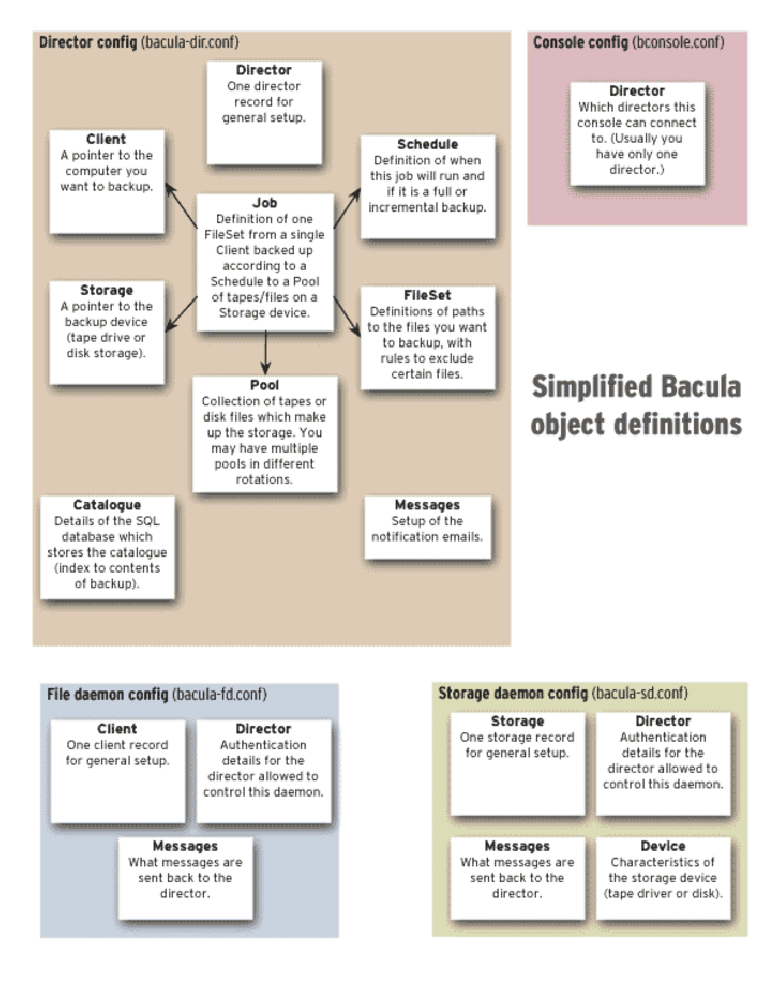
\includegraphics{./bacula-objects.eps} 
\\
(thanks to Aristedes Maniatis for the above graphic) 
\label{ResFormat}

\subsection*{Resource Directive Format}
\index[general]{Resource Directive Format }
\index[general]{Format!Resource Directive }
\addcontentsline{toc}{subsection}{Resource Directive Format}

Although, you won't need to know the details of all the directives a basic
knowledge of Bacula resource directives is essential. Each directive contained
within the resource (within the braces) is composed of a keyword followed by
an equal sign (=) followed by one or more values. The keywords must be one of
the known Bacula resource record keywords, and it may be composed of upper or
lower case characters and spaces. 

Each resource definition MUST contain a Name directive, and may optionally
contain a Description directive (or record). The Name directive is used to
uniquely identify the resource. The Description directive is (will be) used
during display of the Resource to provide easier human recognition. For
example: 

\footnotesize
\begin{verbatim}
Director {
  Name = "MyDir"
  Description = "Main Bacula Director"
  WorkingDirectory = "$HOME/bacula/bin/working"
}
\end{verbatim}
\normalsize

Defines the Director resource with the name ``MyDir'' and a working directory
\$HOME/bacula/bin/working. In general, if you want spaces in a name to the
right of the first equal sign (=), you must enclose that name within double
quotes. Otherwise quotes are not generally necessary because once defined,
quoted strings and unquoted strings are all equal. 
\label{Comments}

\subsubsection*{Comments}
\index[general]{Comments }
\addcontentsline{toc}{subsubsection}{Comments}

When reading the configuration file, blank lines are ignored and everything
after a hash sign (\#) until the end of the line is taken to be a comment. A
semicolon (;) is a logical end of line, and anything after the semicolon is
considered as the next statement. If a statement appears on a line by itself,
a semicolon is not necessary to terminate it, so generally in the examples in
this manual, you will not see many semicolons. 
\label{Case1}

\subsubsection*{Upper and Lower Case and Spaces}
\index[general]{Spaces!Upper and Lower Case and }
\index[general]{Upper and Lower Case and Spaces }
\addcontentsline{toc}{subsubsection}{Upper and Lower Case and Spaces}

Case (upper/lower) and spaces are totally ignored in the resource directive
keywords (the part before the equal sign). 

Within the keyword (i.e. before the equal sign), spaces are not significant.
Thus the keywords: {\bf name}, {\bf Name}, and {\bf N a m e} are all
identical. 

Spaces after the equal sign and before the first character of the value are
ignored. 

In general, spaces within a value are significant (not ignored), and if the
value is a name, you must enclose the name in double quotes for the spaces to
be accepted. Names may contain up to 127 characters. Currently, a name may
contain any ASCII character. Within a quoted string, any character following a
backslash (\textbackslash{}) is taken as itself (handy for inserting
blackslashes and double quotes (``). 

Please note, however, that Bacula resource names as well as certain other
names (e.g. Volume names) will in the future be severely limited to permit
only letters (including ISO accented letters), numbers, and a few special
characters (space, underscore, ...). All other characters and punctuation will
be illegal. 
\label{Includes}

\subsubsection*{Including other Configuration Files}
\index[general]{Including other Configuration Files }
\index[general]{Files!Including other Configuration }
\addcontentsline{toc}{subsubsection}{Including other Configuration Files}

If you wish to break your configuration file into smaller pieces, you can do
so by including other files using the syntax @{\bf filename} where {\bf
filename} is the full path and filename of another file. The @filename
specification can be given anywhere a primitive token would appear. 
\label{DataTypes}

\subsubsection*{Recognized Primitive Data Types}
\index[general]{Types!Recognized Primitive Data }
\index[general]{Recognized Primitive Data Types }
\addcontentsline{toc}{subsubsection}{Recognized Primitive Data Types}

When parsing the resource directives, Bacula classifies the data according to
the types listed below. The first time you read this, it may appear a bit
overwhelming, but in reality, it is all pretty logical and straight forward. 

\begin{description}

\item [name]
   \index[fd]{name }
   A keyword or name consisting of alpha  numeric characters, including the
hyphen, underscore, and dollar  characters. The first character of a {\bf
name} must be  a letter.  A name has a maximum length currently set to 127
bytes.  Typically keywords appear on the left side of an equal (i.e.  they are
Bacula keywords -- i.e. Resource names or  directive names). Keywords may not
be quoted.  

\item [name-string]
   \index[fd]{name-string }
   A name-string is similar to a name,  except that the name may be quoted and
can thus contain  additional characters including spaces. Name strings  are
limited to 127 characters in length. Name strings  are typically used on the
right side of an equal (i.e.  they are values to be associated with a keyword.


\item [string]
   \index[fd]{string }
   A quoted string containing virtually any  character including spaces, or a
non-quoted string. A  string may be of any length. Strings are typically
values  that correspond to filenames, directories, or system  command names. A
backslash (\textbackslash{}) turns the next character into  itself, so to
include a double quote in a string, you precede the  double quote with a
backslash. Likewise to include a backslash. 

\item [directory]
   \index[dir]{directory }
   A directory is either a quoted or  non-quoted string. A directory will be
passed to your  standard shell for expansion when it is scanned. Thus 
constructs such as {\bf \$HOME} are interpreted to be  their correct values. 

\item [password]
   \index[dir]{password }
   This is a Bacula password and  it is stored internally in MD5 hashed format. 

\item [integer]
   \index[dir]{integer }
   A 32 bit integer value. It may be positive  or negative. 

\item [positive integer]
   \index[dir]{positive integer }
   A 32 bit positive integer value. 

\item [long integer]
   \index[dir]{long integer }
   A 64 bit integer value. Typically these  are values such as bytes that can
exceed 4 billion and thus  require a 64 bit value. 

\item [yes|no]
   \index[dir]{yes|no }
   Either a {\bf yes} or a {\bf no}. 

\item [
   \label{Size1}
   size]
\index[dir]{a name }
A size specified as bytes. Typically, this is  a floating point scientific
input format followed by an optional modifier. The  floating point input is
stored as a 64 bit integer value.  If a modifier is present, it must
immediately follow the  value with no intervening spaces. The following
modifiers are permitted:  

\begin{description}

\item [k]
   1,024 (kilobytes)  

\item [kb]
   1,000 (kilobytes)  

\item [m]
   1,048,576 (megabytes)  

\item [mb]
   1,000,000 (megabytes)  

\item [g]
   1,073,741,824 (gigabytes) 

\item [gb]
   1,000,000,000 (gigabytes) 
   \end{description}

\item {\bf 
   \label{Time} 
   time}
\index[dir]{a name }
A time or duration specified in seconds.  The time is stored internally as a
64 bit integer value, but  it is specified in two parts: a number part and a
modifier part.  The number can be an integer or a floating point number. If it
is entered in floating point notation, it will be rounded to  the nearest
integer.  The modifer is mandatory and follows the number part,  either with
or without intervening spaces.  The following modifiers are permitted:

\begin{description}

\item [seconds]
   \index[dir]{seconds }
   seconds  

\item [minutes]
   \index[dir]{minutes }
   minutes (60 seconds)  

\item [hours]
   \index[dir]{hours }
   hours (3600 seconds)  

\item [days]
   \index[dir]{days }
   days (3600*24 seconds)  

\item [weeks]
   \index[dir]{weeks }
   weeks (3600*24*7 seconds)  

\item [months]
   \index[dir]{months }
   months (3600*24*30 seconds)  

\item [quarters]
   \index[dir]{quarters }
   quarters (3600*24*91 seconds)  

\item [years]
   \index[dir]{years }
   years (3600*24*365 seconds)  
\end{description}

Any abbreviation of these modifiers is also permitted (i.e.  {\bf seconds} may
be specified as {\bf sec} or {\bf s}.  A specification of {\bf m} will be
taken as months.  

The specification of a time my have as may number/modifier  parts as you wish.
For example:  

\footnotesize
\begin{verbatim}
1 week 2 days 3 hours 10 mins
1 month 2 days 30 sec
   
\end{verbatim}
\normalsize

are valid date specifications (beginning with version 1.35.1).  

Note! in Bacula version 1.31 and below, the modifier was optional.  It is now
manditory.  
\end{description}

\label{ResTypes}

\subsection*{Resource Types}
\index[general]{Types!Resource }
\index[general]{Resource Types }
\addcontentsline{toc}{subsection}{Resource Types}

The following table lists all current Bacula resource types. It shows what
resources must be defined for each service (daemon). The default configuration
files will already contain at least one example of each permitted resource, so
you need not worry about creating all these kinds of resources from scratch. 

\addcontentsline{lot}{table}{Resource Types}
\begin{longtable}{|l|l|l|l|l|}
 \hline 
\multicolumn{1}{|c| }{\bf Resource } & \multicolumn{1}{c| }{\bf Director } &
\multicolumn{1}{c| }{\bf Client } & \multicolumn{1}{c| }{\bf Storage } &
\multicolumn{1}{c| }{\bf Console  } \\
 \hline 
{Catalog } & {Yes } & {No  } & {No } & {No  } \\
 \hline 
{Client  } & {Yes } & {Yes } & {No } & {No  } \\
 \hline 
{Console } & {Yes } & {No } & {No } & {Yes  } \\
 \hline 
{Device  } & {No  } & {No } & {Yes } & {No  } \\
 \hline 
{Director } & {Yes } & {Yes } & {Yes } & {Yes  } \\
 \hline 
{FileSet } & {Yes } & {No } & {No } & {No  } \\
 \hline 
{Job  } & {Yes } & {No } & {No } & {No  } \\
 \hline 
{JobDefs } & {Yes } & {No } & {No } & {No  } \\
 \hline 
{Message } & {Yes } & {Yes } & {Yes } & {No  } \\
 \hline 
{Pool  } & {Yes } & {No } & {No } & {No  } \\
 \hline 
{Schedule } & {Yes } & {No } & {No } & {No  } \\
 \hline 
{Storage } & {Yes } & {No } & {Yes } & {No }
\\ \hline 

\end{longtable}

\subsection*{Names, Passwords and Authorization}
\label{Names}
\index[general]{Authorization!Names Passwords and }
\index[general]{Names, Passwords and Authorization }
\addcontentsline{toc}{subsection}{Names, Passwords and Authorization}

In order for one daemon to contact another daemon, it must authorize itself
with a password. In most cases, the password corresponds to a particular name,
so both the name and the password must match to be authorized. 

The default configuration files are automatically defined for correct
authorization with random passwords. If you add to or modify these files, you
will need to take care to keep them consistent. 

Here is sort of a picture of what names/passwords in which files/Resources
must match up: 

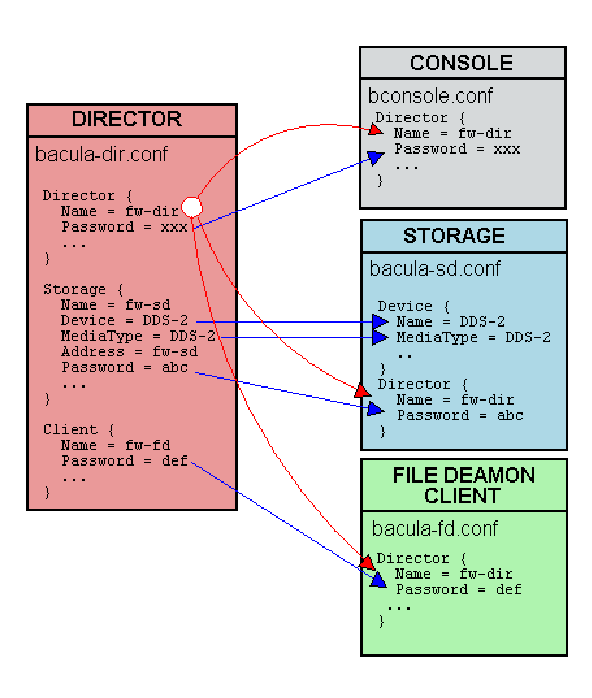
\includegraphics{./Conf-Diagram.eps} 

In the left column, you will find the Director, Storage, and Client resources,
with their names and passwords -- these are all in {\bf bacula-dir.conf}. In
the right column are where the corresponding values should be found in the
Console, Storage daemon (SD), and File daemon (FD) configuration files. 

Please note that the Address, {\bf fd-sd}, that appears in the Storage
resource of the Director, preceded with and asterisk in the above example, is
passed to the File daemon in symbolic form. The File daemon then resolves it
to an IP address. For this reason, you must use either an IP address or a
fully qualified name. A name such as {\bf localhost}, not being a fully
qualified name, will resolve in the File daemon to the localhost of the File
daemon, which is most likely not what is desired. The password used for the
File daemon to authorize with the Storage daemon is a temporary password
unique to each Job created by the daemons and is not specified in any .conf
file. 

\subsection*{Detailed Information for each Daemon}
\index[general]{Detailed Information for each Daemon }
\index[general]{Daemon!Detailed Information for each }
\addcontentsline{toc}{subsection}{Detailed Information for each Daemon}

The details of each Resource and the directives permitted therein are
described in the following chapters. 

The following configuration files must be defined: 

\begin{itemize}
\item 
   \ilink{Console}{_ChapterStart36} -- to define the resources for 
   the Console program (user interface to the Director).  It defines which
Directors are  available so that you may interact with them. 
\item 
   \ilink{Director}{_ChapterStart40} -- to define the resources 
   necessary for the Director. You define all the Clients  and Storage daemons
that you use in this configuration file.  
\item 
   \ilink{Client}{_ChapterStart25} -- to define the resources for 
   each client to be backed up. That is, you will have a separate  Client
resource file on each machine that runs a File daemon. 
\item 
   \ilink{Storage}{_ChapterStart31} -- to define the resources to 
   be used by each Storage daemon. Normally, you will have  a single Storage
daemon that controls your tape drive or tape  drives. However, if you have
tape drives on several machines,  you will have at least one Storage daemon
per machine.  
\end{itemize}

%%
%%

\section*{Configuring the Director}
\label{_ChapterStart40}
\index[general]{Director!Configuring the }
\index[general]{Configuring the Director }
\addcontentsline{toc}{section}{Configuring the Director}

Of all the configuration files needed to run {\bf Bacula}, the Director's is
the most complicated, and the one that you will need to modify the most often
as you add clients or modify the FileSets. 

For a general discussion of configuration file and resources including the
data types recognized by {\bf Bacula}. Please see the 
\ilink{Configuration}{_ChapterStart16} chapter of this manual. 

\subsection*{Director Resource Types}
\index[general]{Types!Director Resource }
\index[general]{Director Resource Types }
\addcontentsline{toc}{subsection}{Director Resource Types}

Director resource type may be one of the following: 

Job, JobDefs, Client, Storage, Catalog, Schedule, FileSet, Pool, Director,  or
Messages. We present them here in the most logical order for defining them: 

\begin{itemize}
\item 
   \ilink{Director}{DirectorResource4} -- to  define the Director's
   name and its access password used for  authenticating the Console program.
Only a single  Director resource definition may appear in the Director's 
configuration file.  If you have either {\bf /dev/random} or  {\bf bc} on your
machine, Bacula will generate a random  password during the configuration
process, otherwise it will  be left blank. 
\item 
   \ilink{Job}{JobResource} -- to define the backup/restore Jobs 
   and to tie together the Client, FileSet and Schedule resources to  be used for
each Job.  
\item 
   \ilink{JobDefs}{JobDefsResource} -- optional resource for 
   providing defaults for Job resources.  
\item 
   \ilink{Schedule}{ScheduleResource} -- to define when a Job is to 
   be automatically run by {\bf Bacula's} internal scheduler.  
\item 
   \ilink{FileSet}{FileSetResource} -- to define the set of files 
   to be backed up for each Client. 
\item 
   \ilink{Client}{ClientResource2} -- to define what Client is  to be
   backed up.  
\item 
   \ilink{Storage}{StorageResource2} -- to define on what  physical
   device the Volumes should be mounted. 
\item 
   \ilink{Pool}{PoolResource} -- to define what  the pool of Volumes
   that can be used for a particular Job. 
\item 
   \ilink{Catalog}{CatalogResource} -- to define in what database to
 keep the list of files and the Volume names where they are backed up.  
\item 
   \ilink{Messages}{_ChapterStart15} -- to define where error  and
   information messages are to be sent or logged. 
\end{itemize}

\subsection*{The Director Resource}
\label{DirectorResource4}
\index[general]{Director Resource }
\index[general]{Resource!Director }
\addcontentsline{toc}{subsection}{Director Resource}

The Director resource defines the attributes of the Directors running on the
network. In the current implementation, there is only a single Director
resource, but the final design will contain multiple Directors to maintain
index and media database redundancy. 

\begin{description}

\item [Director]
   \index[dir]{Director }
   Start of the Director resource. One and only one  director resource must be
supplied.  

\item [Name = \lt{}name\gt{}]
   \index[dir]{Name  }
   The director name used by the system  administrator. This directive is
required.  

\item [Description = \lt{}text\gt{}]
   \index[dir]{Description  }
   The text field contains a  description of the Director that will be displayed
in the  graphical user interface. This directive is optional.  

\item [Password = \lt{}UA-password\gt{}]
   \index[dir]{Password  }
   Specifies the password that  must be supplied for the default Bacula Console
to be  authorized. The same password must appear in the  {\bf Director}
resource of the Console configuration file.  For added security, the password
is never actually passed  across the network but rather a challenge response
hash code  created with the password. This directive is required. If you  have
either {\bf /dev/random} {\bf bc} on your machine,  Bacula will generate a
random password during the  configuration process, otherwise it will be left
blank and  you must manually supply it.  

\item [Messages = \lt{}Messages-resource-name\gt{}]
   \index[dir]{Messages  }
   The messages resource  specifies where to deliver Director messages that are
not associated  with a specific Job. Most messages are specific to a job and
will  be directed to the Messages resource specified by the job. However, 
there are a few messages that can occur when no job is running.  This
directive is required.  

\item [Working Directory = \lt{}Directory\gt{}]
   \index[dir]{Working Directory  }
   This directive  is mandatory and specifies a directory in which the Director 
may put its status files. This directory should be used only  by Bacula but
may be shared by other Bacula daemons.  Standard shell expansion of the {\bf
Directory}  is done when the configuration file is read so that values such 
as {\bf \$HOME} will be properly expanded. This directive is required.  

\item [Pid Directory = \lt{}Directory\gt{}]
   \index[dir]{Pid Directory  }
   This directive  is mandatory and specifies a directory in which the Director 
may put its process Id file files. The process Id file is used to  shutdown
Bacula and to prevent multiple copies of  Bacula from running simultaneously. 
Standard shell expansion of the {\bf Directory}  is done when the
configuration file is read so that values such  as {\bf \$HOME} will be
properly expanded.  

Typically on Linux systems, you will set this to:  {\bf /var/run}. If you are
not installing Bacula in the  system directories, you can use the {\bf Working
Directory} as  defined above.  This directive is required.  

\item [QueryFile = \lt{}Path\gt{}]
   \index[dir]{QueryFile  }
   This directive  is mandatory and specifies a directory and file in which the
Director  can find the canned SQL statements for the {\bf Query} command of 
the Console. Standard shell expansion of the {\bf Path} is done  when the
configuration file is read so that values such as  {\bf \$HOME} will be
properly expanded. This directive is required.  
\label{DirMaxConJobs}

\item [Maximum Concurrent Jobs = \lt{}number\gt{}]
   \index[dir]{Maximum Concurrent Jobs  }
   where \lt{}number\gt{}  is the maximum number of total Director Jobs that
should run  concurrently. The default is set to 1, but you may set it to a 
larger number.  

Please  note that the Volume format becomes much more complicated with 
multiple simultaneous jobs, consequently, restores can take much  longer if
Bacula must sort through interleaved volume blocks from  multiple simultaneous
jobs. This can be avoided by having each  simultaneously running job write to
a different volume or  by using data spooling, which will first spool the data
to disk simultaneously, then write each spool file to the  volume in
sequence.  

There may also still be some cases where directives such as  {\bf Maximum
Volume Jobs} are not properly synchronized with  multiple simultaneous jobs
(subtle timing issues can arise),  so careful testing is recommended. 

At the current time,  there is no configuration parameter set or limit the
number  console connections. A maximum of five simultaneous console 
connections are permitted.  

For more details on getting concurrent jobs to run, please  see 
\ilink{Running Concurrent Jobs}{ConcurrentJobs} in the Tips chapter
of this manual.  

\item [FD Connect Timeout = \lt{}time\gt{}]
   \index[dir]{FD Connect Timeout  }
   where {\bf time}  is the time that the Director should continue attempting  to
contact the File daemon to start a job, and after which the  Director will
cancel the job. The default is 30 minutes. 

\item [SD Connect Timeout = \lt{}time\gt{}]
   \index[dir]{SD Connect Timeout  }
   where {\bf time}  is the time that the Director should continue attempting  to
contact the Storage daemon to start a job, and after which the  Director will
cancel the job. The default is 30 minutes. 

\item [DirAddresses = \lt{}IP-address-specification\gt{}]
   \index[dir]{DirAddresses  }
   Specify the ports and addresses on which the Director daemon will  listen for
Bacula Console connections. Probably the simplest way  to explain is to show
an example: 

\footnotesize
\begin{verbatim}
 DirAddresses  = { ip = {
        addr = 1.2.3.4; port = 1205; }
    ipv4 = {
        addr = 1.2.3.4; port = http; }
    ipv6 = {
        addr = 1.2.3.4;
        port = 1205;
    }
    ip = {
        addr = 1.2.3.4
        port = 1205
    }
    ip = {
        addr = 1.2.3.4
    }
    ip = {
        addr = 201:220:222::2
    }
    ip = {
        addr = bluedot.thun.net
    }
 }
\end{verbatim}
\normalsize

where ip, ip4, ip6, addr, and port are all keywords. Note, that  the address
can be specified as either a dotted quadruple, or  IPv6 colon notation, or as
a symbolic name (only in the ip specification).  Also, port can be specified
as a number or as the mnemonic value from  the /etc/services file.  If a port
is not specified, the default will be used. If an ip  section is specified,
the resolution can be made either by IPv4 or  IPv6. If ip4 is specified, then
only IPv4 resolutions will be permitted,  and likewise with ip6. 

\item [DIRport = \lt{}port-number\gt{}]
   \index[dir]{DIRport  }
   Specify the port (a positive  integer) on which the  Director daemon will
listen for Bacula Console connections.  This same port number must be
specified in the Director resource  of the Console configuration file. The
default is 9101, so  normally this directive need not be specified.  This
directive is not needed if you specify DirAddresses. 

\item [DirAddress = \lt{}IP-Address\gt{}]
   \index[dir]{DirAddress  }
   This directive is optional,  but if it is specified, it will cause the
Director server (for  the Console program) to bind to the specified {\bf
IP-Address},  which is either a domain name or an IP address specified as a 
dotted quadruple in string or quoted string format.  If this directive is not
specified, the Director  will bind to any available address (the default). 
Note, unlike the DirAddresses specification noted above, this  directive only
permits a single address to be specified.  This directive is not needed if you
specify a DirAddresses  (not plural). 
\end{description}

The following is an example of a valid Director resource definition: 

\footnotesize
\begin{verbatim}
Director {
  Name = HeadMan
  WorkingDirectory = "$HOME/bacula/bin/working"
  Password = UA_password
  PidDirectory = "$HOME/bacula/bin/working"
  QueryFile = "$HOME/bacula/bin/query.sql"
  Messages = Standard
}
\end{verbatim}
\normalsize

\subsection*{The Job Resource}
\label{JobResource}
\index[general]{Resource!Job }
\index[general]{Job Resource }
\addcontentsline{toc}{subsection}{Job Resource}

The Job resource defines a Job (Backup, Restore, ...) that Bacula must
perform. Each Job resource definition contains the names of the Clients and
their FileSets to backup or restore, the Schedule for the Job, where the data
are to be stored, and what media Pool can be used. In effect, each Job
resource must specify What, Where, How, and When or FileSet, Storage,
Backup/Restore/Level, and Schedule respectively. 

Only a single type ({\bf Backup}, {\bf Restore}, ...) can be specified for any
job. If you want to backup multiple FileSets on the same Client or multiple
Clients, you must define a Job for each one. 

\begin{description}

\item [Job]
   \index[dir]{Job }
   Start of the Job resource. At least one Job  resource is required. 

\item [Name = \lt{}name\gt{}]
   \index[dir]{Name  }
   The Job name. This name can be specified  on the {\bf Run} command in the
   console program to start a job. If the  name contains spaces, it must be
   specified between quotes. It is  generally a good idea to give your job the
   same name as the Client  that it will backup. This permits easy identification
   of jobs.  

   When the job actually runs, the unique Job Name will consist  of the name you
   specify here followed by the date and time the  job was scheduled for
   execution. This directive is required. 

\item [Type = \lt{}job-type\gt{}]
   \index[dir]{Type  }
   The {\bf Type} directive specifies  the Job type, which may be one of the
following: {\bf Backup},  {\bf Restore}, {\bf Verify}, or {\bf Admin}. This
directive  is required. Within a particular Job Type, there are also Levels 
as discussed in the next item.  

\begin{description}

\item [Backup]
   \index[dir]{Backup }
   Run a backup Job. Normally you will  have at least one Backup job for each
client you want  to save. Normally, unless you turn off cataloging,  most all
the important statistics and data concerning  files backed up will be placed
in the catalog. 

\item [Restore]
   \index[dir]{Restore }
   Run a restore Job. Normally, you will  specify only one Restore job which acts
as a sort  of prototype that you will modify using the console  program in
order to perform restores. Although certain  basic information from a Restore
job is saved in the  catalog, it is very minimal compared to the information 
stored for a Backup job -- for example, no File database  entries are
generated since no Files are saved.  

\item [Verify]
   \index[dir]{Verify }
   Run a verify Job. In general, {\bf verify}  jobs permit you to compare the
contents of the catalog  to the file system, or to what was backed up. In
addition,  to verifying that a tape that was written can be read,  you can
also use {\bf verify} as a sort of tripwire  intrusion detection.  

\item [Admin]
   \index[dir]{Admin }
   Run a admin Job. An {\bf Admin} job can  be used to periodically run catalog
pruning, if you  do not want to do it at the end of each {\bf Backup}  Job.
Although an Admin job is recorded in the  catalog, very little data is saved. 
\end{description}

\label{Level}

\item [Level = \lt{}job-level\gt{}]
   \index[dir]{Level  }
   The Level directive specifies  the default Job level to be run. Each different
Job Type (Backup, Restore, ...) has a different set of Levels  that can be
specified. The Level is normally overridden  by a different value that is
specified in the {\bf Schedule}  resource. This directive is not required, but
must be specified either  by a {\bf Level} directive or as a override
specified in the  {\bf Schedule} resource.  

For a {\bf Backup} Job, the Level may be one of the  following:  

\begin{description}

\item [Full]
   \index[dir]{Full }
   is all files in the FileSet whether or not they  have changed.  

\item [Incremental]
   \index[dir]{Incremental }
   is all files that have changed since the  last successful backup of the
specified FileSet. If the  Director cannot find a previous Full backup then
the job will be  upgraded into a Full backup. When the Director looks for a 
``suitable'' backup record in the catalog database, it  looks for a previous
Job with:  

\begin{itemize}
\item The same Job name.  
\item The same Client name.  
\item The same FileSet (any change to the definition of  the FileSet such as
   adding or deleting a file in the  Include or Exclude sections constitutes a
   different FileSet.  
\item The Job was a Full, Differential, or Incremental backup.  
\item The Job terminated normally (i.e. did not fail or was not  canceled).  
   \end{itemize}

If all the above conditions do not hold, the Director will upgrade  the
Incremental to a Full save. Otherwise, the Incremental  backup will be
performed as requested.  

The File daemon (Client) decides which files to backup for an  Incremental
backup by comparing start time of the prior Job  (Full, Differential, or
Incremental) against the time each file  was last ``modified'' (st\_mtime) and
the time its  attributes were last ``changed''(st\_ctime). If the  file was
modified or its attributes changed on or after this  start time, it will then
be backed up.  

Please note that some  virus scanning software may change st\_ctime while
doing the  scan. For exaple, if the the virus scanning program attempts  to
reset the access time (st\_atime), which Bacula does not use,  it will cause
st\_ctime to change and hence Bacula will backup  the file during an
Incremental or Differential backup. In the  case of Sophos virus scanning, you
can prevent it from  resetting the access time (st\_atime) and hence changing 
st\_ctime by using the {\bf \verb{--{no-reset-atime} option. For  other software,
please see their manual.  

When Bacula does an Incremental backup, all modified  files that are still on
the system are backed up.  However, any file that has been deleted since the
last  Full backup remains in the Bacula catalog, which means  that if between
a Full save and the time you do a  restore, some files are deleted, those
deleted files  will also be restored. The deleted files will no longer  appear
in the catalog after doing another Full save.  However, to remove deleted
files from the catalog during  a Incremental backup is quite a time consuming
process  and not currently implemented in Bacula. 

\item [Differential]
   \index[dir]{Differential }
   is all files that have changed since the  last successful Full backup of the
specified FileSet.  If the Director cannot find a previous Full backup or a 
suitable Full backup, then the Differential job will be  upgraded into a Full
backup. When the Director looks for  a ``suitable'' Full backup record in the
catalog  database, it looks for a previous Job with:  

\begin{itemize}
\item The same Job name.  
\item The same Client name.  
\item The same FileSet (any change to the definition of  the FileSet such as
   adding or deleting a file in the  Include or Exclude sections constitutes a
   different FileSet.  
\item The Job was a FULL backup.  
\item The Job terminated normally (i.e. did not fail or was not  canceled).  
   \end{itemize}

If all the above conditions do not hold, the Director will  upgrade the
Differential to a Full save. Otherwise, the  Differential backup will be
performed as requested.  

The File daemon (Client) decides which files to backup for a  differential
backup by comparing the start time of the prior  Full backup Job against the
time each file was last  ``modified'' (st\_mtime) and the time its attributes
were  last ``changed''(st\_ctime). If the file was modified or  its attributs
were changed on or after this start time, it will  then be backed up. The
start time used is displayed after the  {\bf Since} on the Job report. In rare
cases, using the start  time of the prior backup may cause some files to be
backed up  twice, but it ensures that no change is missed. As with the 
Incremental option, you shouldensure that the clocks on your  server and
client are synchronized or as close as possible to  avoid the possibility of a
file being skipped. Note, on  versions 1.33 or greater Bacula automatically
makes the  necessary adjstments to the time between the server and the  client
so that the times Bacula uses are synchronized.  

When Bacula does an Differential backup, all modified  files that are still on
the system are backed up.  However, any file that has been deleted since the
last  Full backup remains in the Bacula catalog, which means  that if between
a Full save and the time you do a  restore, some files are deleted, those
deleted files  will also be restored. The deleted files will no longer  appear
in the catalog after doing another Full save.  However, to remove deleted
files from the catalog during  a Differential backup is quite a time consuming
process  and not currently implemented in Bacula. 
\end{description}

For a {\bf Restore} Job, no level need be specified.  

For a {\bf Verify} Job, the Level may be one of the  following:  

\begin{description}

\item [InitCatalog]
   \index[dir]{InitCatalog }
   does a scan of the specified {\bf FileSet} and stores the file
   attributes in the Catalog database.  Since no file data is saved, you
   might ask why you would want to do this.  It turns out to be a very
   simple and easy way to have a {\bf Tripwire} like feature using {\bf
   Bacula}.  In other words, it allows you to save the state of a set of
   files defined by the {\bf FileSet} and later check to see if those files
   have been modified or deleted and if any new files have been added.
   This can be used to detect system intrusion.  Typically you would
   specify a {\bf FileSet} that contains the set of system files that
   should not change (e.g.  /sbin, /boot, /lib, /bin, ...).  Normally, you
   run the {\bf InitCatalog} level verify one time when your system is
   first setup, and then once again after each modification (upgrade) to
   your system.  Thereafter, when your want to check the state of your
   system files, you use a {\bf Verify} {\bf level = Catalog}.  This
   compares the results of your {\bf InitCatalog} with the current state of
   the files.

\item [Catalog]
   \index[dir]{Catalog }
   Compares the current state of the files against the state previously
   saved during an {\bf InitCatalog}.  Any discrepancies are reported.  The
   items reported are determined by the {\bf verify} options specified on
   the {\bf Include} directive in the specified {\bf FileSet} (see the {\bf
   FileSet} resource below for more details).  Typically this command will
   be run once a day (or night) to check for any changes to your system
   files.

   Please note!  If you run two Verify Catalog jobs on the same client at
   the same time, the results will certainly be incorrect.  This is because
   Verify Catalog modifies the Catalog database while running in order to
   track new files.

\item [VolumeToCatalog]
   \index[dir]{VolumeToCatalog }
   This level causes Bacula to read  the file attribute data written to the
Volume from the last Job.  The file attribute data are compared to the values
saved in the  Catalog database and any differences are reported. This is 
similar to the {\bf Catalog} level except that instead of  comparing the disk
file attributes to the catalog database, the  attribute data written to the
Volume is read and compared to the  catalog database. Although the attribute
data including the  signatures (MD5 or SHA1) are compared the actual file data
is not  compared (it is not in the catalog). 

Please note! If you  run two Verify VolumeToCatalog jobs on the same client at
the  same time, the results will certainly be incorrect. This is  because the
Verify VolumeToCatalog modifies the Catalog database  while running. 

\item [DiskToCatalog]
   \index[dir]{DiskToCatalog }
   This level causes Bacula to read the  files as they currently are on disk, and
to compare the  current file attributes with the attributes saved in the 
catalog from the last backup for the job specified on  the {\bf VerifyJob}
directive. This level differs from the  {\bf Catalog} level described above by
the fact that it  compare not against a previous Verify job but against a 
previous backup. When you run this level, you must supply the  verify options
on your Include statements. Those options  determine what attribute fields are
compared.  

This command can be very useful if you have disk problems  because it will
compare the current state of your disk against  the last successful backup,
which may be several jobs.  

Note, the current implementation (1.32c) does not  identify files that have
been deleted.  
\end{description}

\item [Verify Job = \lt{}Job-Resource-Name\gt{}]
   \index[dir]{Verify Job  }
   If you run  a verify job without this directive, the last job run will  be
compared with the catalog, which means that you must  immediately follow a
backup by a verify command. If you  specify a {\bf Verify Job} Bacula will
find the last  job with that name that ran. This permits you to run  all your
backups, then run Verify jobs on those that  you wish to be verified (most
often a {\bf VolumeToCatalog})  so that the tape just written is re-read. 

\item [JobDefs = \lt{}JobDefs-Resource-Name\gt{}]
   \index[dir]{JobDefs  }
   If a JobDefs-Resource-Name  is specified, all the values contained in the
named JobDefs resource  will be used as the defaults for the current Job. Any
value that  you explicitly define in the current Job resource, will override 
any defaults specified in the JobDefs resource. The use of this  directive
permits writing much more compact Job resources where the  bulk of the
directives are defined in one or more JobDefs. This  is particularly useful if
you have many similar Jobs but with  minor variations such as different
Clients. A simple example  of the use of JobDefs is provided in the default
bacula-dir.conf  file. 

\item [Bootstrap = \lt{}bootstrap-file\gt{}]
   \index[dir]{Bootstrap  }
   The Bootstrap  directive specifies a bootstrap file that, if provided, will 
be used during {\bf Restore} Jobs and is ignored in other  Job types. The {\bf
bootstrap}  file contains the list of tapes to be used in a restore  Job as
well as which files are to be restored. Specification  of this directive is
optional, and  if specified, it is used only for a restore job. In addition, 
when running a Restore job from the console, this value can  be changed.  

If you use the {\bf Restore} command in the Console program,  to start a
restore job, the {\bf bootstrap}  file will be created automatically from the
files you  select to be restored.  

For additional details of the {\bf bootstrap} file, please see  
\ilink{Restoring Files with the Bootstrap File}{_ChapterStart43} 
chapter of this manual. 

\label{writebootstrap}
\item [Write Bootstrap =  \lt{}bootstrap-file-specification\gt{}]
   \index[dir]{a name }
   The  {\bf writebootstrap} directive specifies a file name where  Bacula will
write a {\bf bootstrap} file for each Backup job  run. Thus this directive
applies only to Backup Jobs. If the Backup  job is a Full save, Bacula will
erase any current contents of  the specified file before writing the bootstrap
records. If the Job  is an Incremental save, Bacula will append the current 
bootstrap record to the end of the file.  

Using this feature,  permits you to constantly have a bootstrap file that can
recover the  current state of your system. Normally, the file specified should
be a mounted drive on another machine, so that if your hard disk is  lost,
you will immediately have a bootstrap record available.  Alternatively, you
should copy the bootstrap file to another machine  after it is updated.  

If the {\bf bootstrap-file-specification} begins with a  vertical bar (|),
Bacula will use the specification as the  name of a program to which it will
pipe the bootstrap record.  It could for example be a shell script that emails
you the  bootstrap record. 

For more details on using this file,  please see the chapter entitled 
\ilink{The Bootstrap File}{_ChapterStart43} of this manual. 

\item [Client = \lt{}client-resource-name\gt{}]
   \index[dir]{Client  }
   The Client directive  specifies the Client (File daemon) that will be used in
   the  current Job. Only a single Client may be specified in any one Job.  The
   Client runs on the machine to be backed up,  and sends the requested files to
   the Storage daemon for backup,  or receives them when restoring. For
   additional details, see the  
   \ilink{Client Resource section}{ClientResource2} of this chapter.
   This directive is required. 

\item [FileSet = \lt{}FileSet-resource-name\gt{}]
   \index[dir]{FileSet  }
   The FileSet directive  specifies the FileSet that will be used in the  current
   Job. The FileSet specifies which directories (or files)  are to be backed up,
   and what options to use (e.g. compression, ...).  Only a single FileSet
   resource may be specified in any one Job.  For additional details, see the  
   \ilink{FileSet Resource section}{FileSetResource} of this
   chapter. This directive is required. 

\item [Messages = \lt{}messages-resource-name\gt{}]
   \index[dir]{Messages  }
   The Messages directive  defines what Messages resource should be used for this
   job, and thus  how and where the various messages are to be delivered. For
   example,  you can direct some messages to a log file, and others can be  sent
   by email. For additional details, see the  
   \ilink{Messages Resource}{_ChapterStart15} Chapter of this 
   manual. This directive is required. 

\item [Pool = \lt{}pool-resource-name\gt{}]
   \index[dir]{Pool  }
   The Pool directive defines  the pool of Volumes where your data can be backed
   up. Many Bacula  installations will use only the {\bf Default} pool. However,
   if  you want to specify a different set of Volumes for different  Clients or
   different Jobs, you will probably want to use Pools.  For additional details,
   see the 
   \ilink{Pool Resource section}{PoolResource} of this chapter. This
   resource is required. 

\item [Full Backup Pool = \lt{}pool-resource-name\gt{}]
   \index[dir]{Full Backup Pool  }
   The {\it Full Backup Pool} specifies a Pool to be used for  Full backups. It
   will override any Pool specification during a  Full backup. This resource is
   optional. 
   
\item [Differential Backup Pool = \lt{}pool-resource-name\gt{}]  
   \index[dir]{Differential Backup Pool  }
   The {\it Differential Backup Pool} specifies a Pool to be used for 
   Differential backups. It will override any Pool specification during a 
   Differentia backup. This resource is optional. 
   
\item [Incremental Backup Pool = \lt{}pool-resource-name\gt{}]  
   \index[dir]{Incremental Backup Pool  }
   The {\it Incremental Backup Pool} specifies a Pool to be used for  Incremental
   backups. It will override any Pool specification during a  Incremental backup.
   This resource is optional. 

\item [Schedule = \lt{}schedule-name\gt{}]
   \index[dir]{Schedule  }
   The Schedule directive defines  what schedule is to be used for the Job. The
   schedule determines  when the Job will be automatically started and what Job
   level (i.e.  Full, Incremental, ...) is to be run. This directive is optional,
   and  if left out, the Job can only be started manually. For additional 
   details, see the 
   \ilink{Schedule Resource Chapter}{ScheduleResource} of this
   manual.  If a Schedule resource is specified, the job will be run according to
   the schedule specified. If no Schedule resource is specified for the  Job,
   the job must be manually started using the Console program.  Although you may
   specify only a single Schedule resource for any one  job, the Schedule
   resource may contain multiple {\bf Run} directives,  which allow you to run
   the Job at many different times, and each  {\bf run} directive permits
   overriding the default Job Level Pool,  Storage, and Messages resources. This
   gives considerable flexibility  in what can be done with a single Job. 

\item [Storage = \lt{}storage-resource-name\gt{}]
   \index[dir]{Storage  }
   The Storage directive  defines the name of the storage services where you want
   to backup  the FileSet data. For additional details, see the 
   \ilink{Storage Resource Chapter}{StorageResource2} of this manual.
    This directive is required.  

\item [Max Start Delay = \lt{}time\gt{}]
   \index[dir]{Max Start Delay  }
   The time specifies  maximum delay between the scheduled time and the actual
   start  time for the Job. For example, a job can be scheduled to run  at
   1:00am, but because other jobs are running, it may wait  to run. If the delay
   is set to 3600 (one hour) and the job  has not begun to run by 2:00am, the job
   will be canceled.  This can be useful, for example, to prevent jobs from
   running  during day time hours. The default is 0 which indicates  no limit. 

\item [Max Run Time = \lt{}time\gt{}]
   \index[dir]{Max Run Time  }
   The time specifies  maximum allowed time that a job may run, counted from the
   when  the job starts ({\bf not} necessarily the same as when the job  was
   scheduled). This directive is implemented only in version 1.33  and later. 

\item [Max Wait Time = \lt{}time\gt{}]
   \index[dir]{Max Wait Time  }
   The time specifies  maximum allowed time that a job may block waiting for a
   resource  (such as waiting for a tape to be mounted, or waiting for the
   storage  or file daemons to perform their duties), counted from the when  the
   job starts ({\bf not} necessarily the same as when the job  was scheduled).
   This directive is implemented only in version 1.33  and later. Note, the
   implementation is not yet complete, so  this directive does not yet work
   correctly. 

\item [Prune Jobs = \lt{}yes|no\gt{}]
   \index[dir]{Prune Jobs  }
   Normally, pruning of Jobs  from the Catalog is specified on a Client by Client
   basis in the  Client resource with the {\bf AutoPrune} directive. If this 
   directive is specified (not normally) and the value is {\bf yes}, it  will
   override the value specified in the Client resource.  The default is {\bf no}.


\item [Prune Files = \lt{}yes|no\gt{}]
   \index[dir]{Prune Files  }
   Normally, pruning of Files  from the Catalog is specified on a Client by
Client basis in the  Client resource with the {\bf AutoPrune} directive. If
this  directive is specified (not normally) and the value is {\bf yes}, it 
will override the value specified in the Client resource.  The default is {\bf
no}. 

\item [Prune Volumes = \lt{}yes|no\gt{}]
   \index[dir]{Prune Volumes  }
   Normally, pruning of Volumes  from the Catalog is specified on a Client by
   Client basis in the  Client resource with the {\bf AutoPrune} directive. If
   this  directive is specified (not normally) and the value is {\bf yes}, it 
   will override the value specified in the Client resource.  The default is {\bf
   no}. 

\item [Run Before Job = \lt{}command\gt{}]
   \index[dir]{Run Before Job  }
   The specified {\bf command}  is run as an external program prior to running
   the current Job. Any  output sent by the job to standard output will be
   included in the  Bacula job report. The command string must be a valid program
   name  or name of a shell script. This directive is not required, but if it is 
   defined, and if the exit code of the program run is non-zero, the  current
   Bacula job will be canceled. In addition, the command string  is parsed then
   feed to the execvp() function, which means that the  path will be searched to
   execute your specified command, but there  is no shell interpretation, as a
   consequence, if you  complicated commands or want any shell features such as
   redirection  or piping, you must call a shell script and do it inside  that
   script.  
 
   Before submitting the specified command to the operating system,  Bacula
   performs character substitution of the following  characters:  
  
\footnotesize
\begin{verbatim}
    %% = %
    %c = Client's name
    %d = Director's name
    %i = JobId
    %e = Job Exit Status
    %j = Unique Job name
    %l = Job Level
    %n = Job name
    %t = Job type
    %v = Volume name
    
\end{verbatim}
\normalsize

The Job Exit Status code \%e edits the following values:

\begin{itemize}
\item OK
\item Error
\item Fatal Error
\item Canceled
\item Differences
\item Unknown term code
\end{itemize}

   Thus if you edit it on a command line, you will need to enclose 
   it within some sort of quotes.
   
   Bacula checks the exit status of the RunBeforeJob 
   program. If it is non-zero, the job will be error terminated.  Lutz Kittler
   has pointed out that this can be a simple way to modify  your schedules during
   a holiday. For example, suppose that you normally  do Full backups on Fridays,
   but Thursday and Friday are holidays. To avoid  having to change tapes between
   Thursday and Friday when no one is in the  office, you can create a
   RunBeforeJob that returns a non-zero status on  Thursday and zero on all other
   days. That way, the Thursday job will not  run, and on Friday the tape you
   insert on Wednesday before leaving will  be used.  

\item [Run After Job = \lt{}command\gt{}]
   \index[dir]{Run After Job  }
   The specified {\bf command}  is run as an external program after the current
   job terminates.  This directive is not required. The  command string must be a
   valid program name or name of a shell script.  If the exit code of the program
   run is non-zero, the current  Bacula job will terminate in error.  Before
   submitting the specified command to the operating system,  Bacula performs
   character substitution as described above  for the {\bf Run Before Job}
   directive.  
   
   An example of the use of this command is given in the  
   \ilink{Tips Chapter}{JobNotification} of this manual.  As of version
   1.30, Bacula checks the exit status of the RunAfter  program. If it is
   non-zero, the job will be terminated in error.  

\item [Client Run Before Job = \lt{}command\gt{}]
   \index[dir]{Client Run Before Job  }
   This command  is the same as {\bf Run Before Job} except that it is  run on
   the client machine. The same restrictions apply to  Unix systems as noted
   above for the {\bf Run Before Job}. In  addition, for a Windows client on
   version 1.33 and above, please  take careful note that you must ensure a
   correct path to your  script, and the script or program can be a .com, .exe or
   a .bat  file. However, if you specify a path, you must also specify  the full
   extension. Unix like commands will not work unless you  have installed and
   properly configured Cygwin in addition to  and separately from Bacula.  
   
   {\bf Special Windows Considerations}
   The command can be anything that cmd.exe or command.com will  recognize as a
   executable file. Specifiying the executable's  extention is optional, unless
   there is an ambiguity. (i.e.  ls.bat, ls.exe)  
   
   The System \%Path\% will be searched for the command. (under  the envrionment
   variable dialog you have have both System  Environment and User Environment,
   we believe that only the  System environment will be available to bacual-fd,
   if it is  running as a service.)  
   
   System environment varaible can be called out using the \%var\%  syntax and
   used as either part of the command name or  arguments.  
   
   When specifiying a full path to an executable if the path or  executable name
   contains whitespace or special characters they  will need to be quoted.
   Arguments containing whitespace or  special characters will also have to be
   quoted. 

\footnotesize
\begin{verbatim}
ClientRunBeforeJob = "\"C:/Program Files/Software
     Vendor/Executable\" /arg1 /arg2 \"foo bar\""
\end{verbatim}
\normalsize

   The special characters \&()[]\{\}\^{}=;!'+,`\~{} will need to be quoted  if
   part of a filename or argument.  
   
   If someone is logged in a blank ``command'' window running the  commands will
   be present during the execution of the command.  
   
   Some Suggestions from Phil Stracchino for running on Win32 machines  with the
   native Win32 File daemon: 

   \begin{enumerate}
   \item You might want the ClientRunBeforeJob directive to specify a .bat file
      which  runs the actual client-side commands, rather than trying to run (for 
      example) regedit /e directly.  
   \item The batch file should explicitly 'exit 0' on successful completion.  
   \item The path to the batch file should be specified in Unix form:  
   
      ClientRunBeforeJob = ``c:/bacula/bin/systemstate.bat''  
   
   rather than DOS/Windows form:  
   
   ClientRunBeforeJob =
   ``c:\textbackslash{}bacula\textbackslash{}bin\textbackslash{}systemstate.bat''
   INCORRECT 
   \end{enumerate}

\item [Client Run After Job = \lt{}command\gt{}]
   \index[dir]{Client Run After Job  }
   This command  is the same as {\bf Run After Job} except that it is  run on the
   client machine. Note, please see the notes above  in {\bf Client Run Before
   Job} concerning Windows clients. 

\item [Rerun Failed Levels = \lt{}yes|no\gt{}]
   \index[dir]{Rerun Failed Levels  }
   If this directive  is set to {\bf yes} (default no), and Bacula detects that a
   previous job at a higher level (i.e. Full or Differential)  has failed, the
   current job level will be upgraded to the  higher level. This is particularly
   useful for Laptops where  they may often be unreachable, and if a prior Full
   save has  failed, you wish the very next backup to be a Full save  rather than
   whatever level it is started as. 

\item [Spool Data = \lt{}yes|no\gt{}]
   \index[dir]{Spool Data  }
   If this directive is set  to {\bf yes} (default no), the Storage daemon will
be requested  to spool the data for this Job to disk rather than write it 
directly to tape. Once all the data arrives or the spool file  maximum sizes
are reached, the data will be despooled and written  to tape. When this
directive is set to yes, the Spool Attributes  is also automatically set to
yes. Spooling data prevents tape  shoe-shine (start and stop) during
Incremental saves. This option  should not be used if you are writing to a
disk file. 

\item [Spool Attributes = \lt{}yes|no\gt{}]
   \index[dir]{Spool Attributes  }
   The default is set to  {\bf no}, which means that the File attributes are sent
by the  Storage daemon to the Director as they are stored on tape. However, 
if you want to avoid the possibility that database updates will  slow down
writing to the tape, you may want to set the value to  {\bf yes}, in which
case the Storage daemon will buffer the  File attributes and Storage
coordinates to a temporary file  in the Working Directory, then when writing
the Job data to the tape is  completed, the attributes and storage coordinates
will be  sent to the Director. The default is {\bf no}. 

\item [Where = \lt{}directory\gt{}]
   \index[dir]{Where  }
   This directive applies only  to a Restore job and specifies a prefix to the
directory name  of all files being restored. This permits files to be restored
in a different location from which they were saved. If {\bf Where}  is not
specified or is set to backslash ({\bf /}), the files  will be restored to
their original location. By default, we  have set {\bf Where} in the example
configuration files to be  {\bf /tmp/bacula-restores}. This is to prevent
accidental overwriting  of your files. 

\item [Replace = \lt{}replace-option\gt{}]
   \index[dir]{Replace  }
   This directive applies only  to a Restore job and specifies what happens when
Bacula wants to  restore a file or directory that already exists. You have the
 following options for {\bf replace-option}:  

\begin{description}

\item [always]
   \index[dir]{always }
  when the file to be restored already exists,  it is deleted then replaced by
  the copy backed up.  

\item [ifnewer]
   \index[dir]{ifnewer }
  if the backed up file (on tape) is newer than the  existing file, the existing
  file is deleted and replaced by  the back up.  

\item [ifolder]
   \index[dir]{ifolder }
  if the backed up file (on tape) is older than the  existing file, the existing
  file is deleted and replaced by  the back up.  

\item [never]
   \index[dir]{never }
  if the backed up file already exists, Bacula skips  restoring this file.  
\end{description}

\item [Prefix Links=\lt{}yes|no\gt{}]
   \index[dir]{Prefix Links }
   If a {\bf Where} path prefix is specified for a recovery job, apply it
   to absolute links as well.  The default is {\bf No}.  When set to {\bf
   Yes} then while restoring files to an alternate directory, any absolute
   soft links will also be modified to point to the new alternate
   directory.  Normally this is what is desired -- i.e.  everything is self
   consistent.  However, if you wish to later move the files to their
   original locations, all files linked with absolute names will be broken.

\item [Maximum Concurrent Jobs = \lt{}number\gt{}]
   \index[dir]{Maximum Concurrent Jobs  }
   where \lt{}number\gt{}  is the maximum number of Jobs from the current Job
resource that  can run concurrently. Note, this directive limits only Jobs 
with the same name as the resource in which it appears. Any  other
restrictions on the maximum concurrent jobs such as in  the Director, Client,
or Storage resources will also apply in addition to  the limit specified here.
The  default is set to 1, but you may set it to a larger number.  We strongly
recommend that you read the WARNING documented under  
\ilink{ Maximum Concurrent Jobs}{DirMaxConJobs} in the Director's
resource.  

\item [Reschedule On Error = \lt{}yes|no\gt{}]
   \index[dir]{Reschedule On Error  }
   If this directive is enabled,  and the job terminates in error, the job will
be rescheduled as determined  by the {\bf Reschedule Interval} and {\bf
Reschedule Times} directives.  If you cancel the job, it will not be
rescheduled. The default is  {\bf no} (i.e. the job will not be rescheduled). 


This specification can be useful for portables, laptops, or other  machines
that are not always connected to the network or switched on.  

\item [Reschedule Interval = \lt{}time-specification\gt{}]
   \index[dir]{Reschedule Interval  }
   If you have  specified {\bf Reschedule On Error = yes} and the job terminates
in  error, it will be rescheduled after the interval of time specified  by
{\bf time-specification}. See 
\ilink{ the time specification formats}{Time} in the Configure
chapter for  details of time specifications. If no interval is specified, the 
job will not be rescheduled on error. 

\item [Reschedule Times = \lt{}count\gt{}]
   \index[dir]{Reschedule Times  }
   This directive specifies the  maximum number of times to reschedule the job.
If it is set to zero  (the default) the job will be rescheduled an indefinite
number of times.  
\label{Priority}

\item [Priority = \lt{}number\gt{}]
   \index[dir]{Priority  }
   This directive permits you  to control the order in which your jobs run by
specifying a positive  non-zero number. The higher the number, the lower the
job priority.  Assuming you are not running concurrent jobs, all queued jobs
of  priority 1 will run before queued jobs of priority 2 and so on, 
regardless of the original scheduling order.  

The priority only affects waiting jobs that are queued to run, not jobs  that
are already running. If one or more jobs of priority 2 are already  running,
and a new job is scheduled with priority 1, the currently  running priority 2
jobs must complete before the priority 1 job is run.  

The default priority is 10.  

If you want to run concurrent jobs, which is not recommended, you should  keep
these points in mind:  

\begin{itemize}
\item To run concurrent jobs,  you must set Maximum Concurrent Jobs = 2 in 5
   or 6 distinct places:  in bacula-dir.conf in the Director, the Job, the
   Client, the Storage  resources; in bacula-fd in the FileDaemon (or Client)
   resource,  and in bacula-sd.conf in the Storage resource. If any one  is
   missing, it will throttle the jobs to one at a time.  
\item Bacula concurrently runs jobs of only one priority at a time. It will 
   not simultaneously run a priority 1 and a priority 2 job.  
\item If Bacula is running a priority 2 job and a new priority 1  job is
   scheduled, it will wait until the running priority 2 job  terminates even if
   the Maximum Concurrent Jobs settings  would otherwise allow two jobs to run
   simultaneously.  
\item Suppose that bacula is running a priority 2 job and new priority 1  job
   is scheduled and queued waiting for the running priority  2 job to terminate.
   If you then start a second priority 2 job,  the waiting priority 1 job  will
   prevent the new priority 2 job from running concurrently  with the running
   priority 2 job.  That is: as long as there is a higher priority job waiting to
   run, no new lower priority jobs will start even if  the Maximum Concurrent
   Jobs settings would normally allow  them to run. This ensures that higher
   priority jobs will  be run as soon as possible. 
\end{itemize}

If you have several jobs of different priority, it is best  not to start them
at exactly the same time, because Bacula  must examine them one at a time. If
by chance Bacula treats  a lower priority first, then it will run before your
high  priority jobs. To avoid this, start any higher priority  a few seconds
before lower ones. This insures that Bacula  will examine the jobs in the
correct order, and that your  priority scheme will be respected.  

\end{description}

The following is an example of a valid Job resource definition: 

\footnotesize
\begin{verbatim}
Job {
  Name = "Minou"
  Type = Backup
  Level = Incremental                 # default
  Client = Minou
  FileSet="Minou Full Set"
  Storage = DLTDrive
  Pool = Default
  Schedule = "MinouWeeklyCycle"
  Messages = Standard
}
\end{verbatim}
\normalsize

\subsection*{The JobDefs Resource}
\label{JobDefsResource}
\index[general]{JobDefs Resource }
\index[general]{Resource!JobDefs }
\addcontentsline{toc}{subsection}{JobDefs Resource}

The JobDefs resource permits all the same directives that can appear in a Job
resource. However, a JobDefs resource does not create a Job, rather it can be
referenced within a Job to provide defaults for that Job. This permits you to
concisely define several nearly identical Jobs, each one referencing a JobDefs
resource which contains the defaults. Only the changes from the defaults need
be mentioned in each Job. 

\subsection*{The Schedule Resource}
\label{ScheduleResource}
\index[general]{Resource!Schedule }
\index[general]{Schedule Resource }
\addcontentsline{toc}{subsection}{Schedule Resource}

The Schedule resource provides a means of automatically scheduling a Job as
well as the ability to override the default Level, Pool, Storage and Messages
resources. If a Schedule resource is not referenced in a Job, the Job may only
be run manually. In general, you specify an action to be taken and when. 

\begin{description}

\item [Schedule]
   \index[dir]{Schedule }
   Start of the Schedule directives. No {\bf Schedule}  resource is required, but
you will need at least one if you want  Jobs to be automatically started. 

\item [Name = \lt{}name\gt{}]
   \index[dir]{Name  }
   The name of the schedule being defined.  The Name directive is required. 

\item [Run = \lt{}Job-overrides\gt{} \lt{}Date-time-specification\gt{}]
   \index[dir]{Run  }
   The Run directive defines when a Job is to be run,  and what overrides if any
to apply. You may specify multiple  {\bf run} directives within a {\bf
Schedule} resource. If you  do, they will all be applied (i.e. multiple
schedules). If you  have two {\bf Run} directives that start at the same time,
two  Jobs will start at the same time (well, within one second of  each
other).  

The {\bf Job-overrides} permit overriding the Level, the  Storage, the
Messages, and the Pool specifications  provided in the Job resource. In
addition, the  FullPool, the IncrementalPool, and the  DifferentialPool
specifications permit overriding the  Pool specification according to what
backup Job Level is  in effect.  

By the use of overrides, you  may customize a particular Job. For example, you
may specify a  Messages override for your Incremental backups that  outputs
messages to a log file, but for your weekly or monthly  Full backups, you may
send the output by email by using  a different Messages override.  

{\bf Job-overrides} are specified as:  {\bf keyword=value} where the keyword
is Level, Storage,  Messages, Pool, FullPool, DifferentialPool, or
IncrementalPool, and  the {\bf value} is as defined on the respective
directive formats for  the Job resource. You may specify multiple {\bf
Job-overrides} on  one {\bf Run} directive by separating them with one or more
spaces or  by separating them with a trailing comma.  For example:  

\begin{description}

\item [Level=Full]
   \index[dir]{Level }
   is all files in the FileSet whether or not  they have changed.  

\item [Level=Incremental]
   \index[dir]{Level }
   is all files that have changed since  the last backup.  

\item [Pool=Weekly]
   \index[dir]{Pool }
   specifies to use the Pool named {\bf Weekly}.  

\item [Storage=DLT\_Drive]
   \index[dir]{Storage }
   specifies to use {\bf DLT\_Drive} for  the storage device.  

\item [Messages=Verbose]
   \index[dir]{Messages }
   specifies to use the {\bf Verbose}  message resource for the Job.  

\item [FullPool=Full]
   \index[dir]{FullPool }
   specifies to use the Pool named {\bf Full}  if the job is a full backup, or is
upgraded from another type  to a full backup.  

\item [DifferentialPool=Differential]
   \index[dir]{DifferentialPool }
   specifies to use the Pool  named {\bf Differential} if the job is a
differential  backup.  

\item [IncrementalPool=Incremental]
   \index[dir]{IncrementalPool }
   specifies to use the Pool  named {\bf Incremental} if the job is an
incremental  backup.  

\item [SpoolData=yes|no]
   \index[dir]{SpoolData }
   tells Bacula to request the Storage  daemon to spool data to a disk file
before putting it on  tape.  

\item [WritePartAfterJob=yes|no]
   \index[dir]{WritePartAfterJob }
   tells Bacula to request the Storage  daemon to write the current part file to
   the device when the job  is finished (see 
   \ilink{Write Part After Job directive in the Job
   resource}{WritePartAfterJob}). Please note, this directive is implemented 
   only in version 1.37 and later.

\end{description}

{\bf Date-time-specification} determines when the  Job is to be run. The
specification is a repetition, and as  a default Bacula is set to run a job at
the beginning of the  hour of every hour of every day of every week of every
month  of every year. This is not normally what you want, so you  must specify
or limit when you want the job to run. Any  specification given is assumed to
be repetitive in nature and  will serve to override or limit the default
repetition. This  is done by specifing masks or times for the hour, day of the
month, day of the week, week of the month, week of the year,  and month when
you want the job to run. By specifying one or  more of the above, you can
define a schedule to repeat at  almost any frequency you want.  

Basically, you must supply a {\bf month}, {\bf day}, {\bf hour}, and  {\bf
minute} the Job is to be run. Of these four items to be specified,  {\bf day}
is special in that you may either specify a day of the month  such as 1, 2,
... 31, or you may specify a day of the week such  as Monday, Tuesday, ...
Sunday. Finally, you may also specify a  week qualifier to restrict the
schedule to the first, second, third,  fourth, or fifth week of the month.  

For example, if you specify only a day of the week, such as {\bf Tuesday}  the
Job will be run every hour of every Tuesday of every Month. That  is the {\bf
month} and {\bf hour} remain set to the defaults of  every month and all
hours.  

Note, by default with no other specification, your job will run  at the
beginning of every hour. If you wish your job to run more than  once in any
given hour, you will need to specify multiple {\bf run}  specifications each
with a different minute.  

The date/time to run the Job can be specified in the following way  in
pseudo-BNF:  

\footnotesize
\begin{verbatim}
<void-keyword>    = on
<at-keyword>      = at
<week-keyword>    = 1st | 2nd | 3rd | 4th | 5th | first |
                    second | third | forth | fifth
<wday-keyword>    = sun | mon | tue | wed | thu | fri | sat |
                    sunday | monday | tuesday | wednesday |
                    thursday | friday
<week-of-year-keyword> = w00 | w01 | ... w52 | w53
<month-keyword>   = jan | feb | mar | apr | may | jun | jul |
                    aug | sep | oct | nov | dec | january |
                    february | ... | december
<daily-keyword>   = daily
<weekly-keyword>  = weekly
<monthly-keyword> = monthly
<hourly-keyword>  = hourly
<digit>           = 1 | 2 | 3 | 4 | 5 | 6 | 7 | 8 | 9 | 0
<number>          = <digit> | <digit><number>
<12hour>          = 0 | 1 | 2 | ... 12
<hour>            = 0 | 1 | 2 | ... 23
<minute>          = 0 | 1 | 2 | ... 59
<day>             = 1 | 2 | ... 31
<time>            = <hour>:<minute> |
                    <12hour>:<minute>am |
                    <12hour>:<minute>pm
<time-spec>       = <at-keyword> <time> |
                    <hourly-keyword>
<date-keyword>    = <void-keyword>  <weekly-keyword>
<day-range>       = <day>-<day>
<month-range>     = <month-keyword>-<month-keyword>
<wday-range>      = <wday-keyword>-<wday-keyword>
<range>           = <day-range> | <month-range> |
                          <wday-range>
<date>            = <date-keyword> | <day> | <range>
<date-spec>       = <date> | <date-spec>
<day-spec>        = <day> | <wday-keyword> |
                    <day-range> | <wday-range> |
                    <daily-keyword>
<day-spec>        = <day> | <wday-keyword> |
                    <week-keyword> <wday-keyword>
<month-spec>      = <month-keyword> | <month-range> |
                    <monthly-keyword>
<date-time-spec>  = <month-spec> <day-spec> <time-spec>
\end{verbatim}
\normalsize

\end{description}

Note, the Week of Year specification wnn follows the ISO standard definition
of the week of the year, where Week 1 is the week in which the first Thursday
of the year occurs, or alternatively, the week which contains the 4th of
January. Weeks are numbered w01 to w53. w00 for Bacula is the week that
precedes the first ISO week (i.e. has the first few days of the year if any
occur before Thursday). w00 is not defined by the ISO specification. A week
starts with Monday and ends with Sunday. 

An example schedule resource that is named {\bf WeeklyCycle} and runs a job
with level full each Sunday at 1:05am and an incremental job Monday through
Saturday at 1:05am is: 

\footnotesize
\begin{verbatim}
Schedule {
  Name = "WeeklyCycle"
  Run = Level=Full sun at 1:05
  Run = Level=Incremental mon-sat at 1:05
}
\end{verbatim}
\normalsize

An example of a possible monthly cycle is as follows: 

\footnotesize
\begin{verbatim}
Schedule {
  Name = "MonthlyCycle"
  Run = Level=Full Pool=Monthly 1st sun at 1:05
  Run = Level=Differential 2nd-5th sun at 1:05
  Run = Level=Incremental Pool=Daily mon-sat at 1:05
}
\end{verbatim}
\normalsize

The first of every month: 

\footnotesize
\begin{verbatim}
Schedule {
  Name = "First"
  Run = Level=Full on 1 at 1:05
  Run = Level=Incremental on 2-31 at 1:05
}
\end{verbatim}
\normalsize

Every 10 minutes: 

\footnotesize
\begin{verbatim}
Schedule {
  Name = "TenMinutes"
  Run = Level=Full hourly at 0:05
  Run = Level=Full hourly at 0:15
  Run = Level=Full hourly at 0:25
  Run = Level=Full hourly at 0:35
  Run = Level=Full hourly at 0:45
  Run = Level=Full hourly at 0:55
}
\end{verbatim}
\normalsize

\subsection*{Technical Notes on Schedules}
\index[general]{Schedules!Technical Notes on }
\index[general]{Technical Notes on Schedules }
\addcontentsline{toc}{subsection}{Technical Notes on Schedules}

Internally Bacula keeps a schedule as a bit mask. There are six masks and a
minute field to each schedule. The masks are hour, day of the month (mday),
month, day of the week (wday), week of the month (wom), and week of the year
(woy). The schedule is initialized to have the bits of each of these masks
set, which means that at the beginning of every hour, the job will run. When
you specify a month for the first time, the mask will be cleared and the bit
corresponding to your selected month will be selected. If you specify a second
month, the bit corresponding to it will also be added to the mask. Thus when
Bacula checks the masks to see if the bits are set corresponding to the
current time, your job will run only in the two months you have set. Likewise,
if you set a time (hour), the hour mask will be cleared, and the hour you
specify will be set in the bit mask and the minutes will be stored in the
minute field. 

For any schedule you have defined, you can see how these bits are set by doing
a {\bf show schedules} command in the Console program. Please note that the
bit mask is zero based, and Sunday is the first day of the week (bit zero). 

%%
%%

\subsection*{The FileSet Resource}
\label{FileSetResource}
\index[general]{Resource!FileSet }
\index[general]{FileSet Resource }
\addcontentsline{toc}{subsection}{FileSet Resource}

The FileSet resource defines what files are to be included or excluded in a
backup job.  A {\bf FileSet} resource is required for each backup Job.  It
consists of a list of files or directories to be included, a list of files
or directories to be excluded and the various backup options such as
compression, encryption, and signatures that are to be applied to each
file.

Any change to the list of the included files will cause Bacula to
automatically create a new FileSet (defined by the name and an MD5 checksum
of the Include/Exclude contents).  Each time a new FileSet is created,
Bacula will ensure that the next backup is always a Full save.

\begin{description}

\item [FileSet]
\index[dir]{FileSet }
Start of the FileSet resource. One {\bf FileSet}  resource must be
defined for each Backup job.

\item [Name = \lt{}name\gt{}]
\index[dir]{Name  }
The name of the FileSet resource.  This directive is required. 

\item [Ignore FileSet Changes = \lt{}yes|no\gt{}]
\index[dir]{Ignore FileSet Changes  }
   If this directive is set to {\bf yes}, any changes you make to the  FileSet
   Include or Exclude lists will be ignored and not cause Bacula  to immediately
   perform a Full backup. The default is {\bf no}, in which  case, if you change
   the Include or Exclude, Bacula will force a Full  backup to ensure that
   everything is properly backed up. It is not recommended  to set this directive
   to yes. This directive is available in Bacula  version 1.35.4 or later. 

\item [Include \{ Options \{\lt{}file-options\gt{}\} ...;
   \lt{}file-list\gt{} \} ]
\index[dir]{Include \  \{ [ Options \{\lt{}file-options\gt{}\} ...]
   \lt{}file-list\gt{} \}  }

\item [Options \ \{ \lt{}file-options\gt{} \} ]
\index[dir]{Options \  \{ \lt{}file-options\gt{} \}  }

\item [Exclude \ \{ \lt{}file-list\gt{} \}]
\index[dir]{Exclude \  \{ \lt{}file-list\gt{} \} }

\end{description}

The Include resource must contain a list of directories and/or files to be
processed in the backup job.  Normally, all files found in all
subdirectories of any directory in the Include File list will be backed up.
The Include resource may also contain one or more Options resources that
specify options such as compression to be applied to all or any subset of
the files found for backup.

There can be any number of {\bf Include} resources within the FileSet, each
having its own list of directories or files to be backed up and the backup
options defined by one or more Options resources.  The {\bf file-list}
consists of one file or directory name per line.  Directory names should be
specified without a trailing slash with Unix path notation.

You should always specify a full path for every directory and file that you
list in the FileSet.  In addition, on Windows machines, you should {\bf
always} prefix the directory or filename with the drive specification in
lower case (e.g.  {\bf c:/xxx}) using Unix directory name separators
(forward slash).

Bacula's default for processing directories is to recursively descend in
the directory saving all files and subdirectories.  Bacula will not by
default cross filesystems (or mount points in Unix parlance).  This means
that if you specify the root partition (e.g.  {\bf /}), Bacula will save
only the root partition and not any of the other mounted filesystems.
Similarly on Windows systems, you must explicitly specify each of the
drives you want saved (e.g.
{\bf c:/} and {\bf d:/} ...). In addition, at least for Windows systems, you
will most likely want to enclose each specification within double quotes
particularly if the directory (or file) name contains spaces. The {\bf df}
command on Unix systems will show you which mount points you must specify to
save everything. See below for an example. 

Take special care not to include a directory twice or Bacula will backup
the same files two times wasting a lot of space on your archive device.
Including a directory twice is very easy to do.  For example:

\footnotesize
\begin{verbatim}
  Include {
    File = /
    File = /usr
    Options { compression=GZIP }
  }
\end{verbatim}
\normalsize

on a Unix system where /usr is a subdirectory (rather than a mounted
filesystem) will cause /usr to be backed up twice. In this case, on Bacula
versions prior to 1.32f-5-09Mar04 due to a bug, you will not be able to
restore hard linked files that were backed up twice. 

If you have used Bacula prior to version 1.34.3, you will note three things in
the new FileSet syntax: 

\begin{enumerate}
\item There is no equal sign (=) after the Include and before the opening
   brace (\{). The same is true for the Exclude. 
\item Each directory (or filename) to be included or excluded is preceded by a {\bf File
   =}.  Previously they were simply listed on separate lines. 
\item The options that previously appeared on the Include line now must be
   specified within their own Options resource.
\item The Exclude resource does not accept Options. 
\item When using wild-cards or regular expressions, directory names are
   always terminated with a slash (/) and filenames have no trailing slash.
\end{enumerate}

The Options resource is optional, but when specified, it will contain a
list of {\bf keyword=value} options to be applied to the file-list.
Multiple Options resources may be specified one after another.  As the
files are found in the specified directories, the Options will applied to
the filenames to determine if and how the file should be backed up.  The
Options resources are applied in the order they are specified in the
FileSet until the first one that matches.  

Once Bacula determines that the Options resource matches the file under
consideration, that file will be saved without looking at any other Options
resources that may be present.  This means that any wild cards must appear
before an Options resource without wild cards.

If for some reason, Bacula applies all the Options resources to a file
under consideration for backup, but there are no matches (generally because
of wild cards that don't match), Bacula as a default will then backup the
file.  This is quite logical if you consider the case of no Options, where
you want everything to be backed up.  

However, one additional point is that
in the case that no match was found, Bacula will use the options found in
the last Options resource.  As a consequence, if you want a particular set
of ``default'' options, you should put them in an Options resource after
any other Options.

This is perhaps a bit overwhelming, so there are a number of examples included 
below to illustrate how this works.

The directives within an Options resource may be one of the following: 

\begin{description}

\item [compression=GZIP]
\index[fd]{compression }
   All files saved will be software compressed using the GNU ZIP compression
   format. The  compression is done on a file by file basis by the File daemon. 
   If there is a problem reading the tape in a  single record of a file, it will
   at most affect that file and none  of the other files on the tape. Normally
   this option is {\bf not} needed  if you have a modern tape drive as the drive
   will do its own  compression. In fact, if you specify software compression at
   the same time you have hardware compression turned on, your files  may
   actually take more space on the volume.  

   Software compression is very important if you are writing  your Volumes to a
   file, and it can also be helpful if you have a fast computer but a slow
   network, otherwise it is generally better to rely your tape drive's hardware
   compression. As noted above, it is not generally a good idea to do both software 
   and hardware compression.

   Specifying {\bf GZIP} uses the default compression level six (i.e. {\bf GZIP}
   is identical to {\bf GZIP6}). If you  want a different compression level (1
   through 9), you can specify  it by appending the level number with no
   intervening spaces  to {\bf GZIP}. Thus {\bf compression=GZIP1} would give
   minimum  compression but the fastest algorithm, and {\bf compression=GZIP9} 
   would give the highest level of compression, but requires more  computation.
   According to the GZIP documentation, compression levels  greater than 6
   generally give very little extra compression and are rather CPU intensive. 

\item [signature=SHA1]
\index[fd]{signature }
   An SHA1 signature will be computed for all  The SHA1 algorithm is purported to
   be some  what slower than the MD5 algorithm, but at the same time is 
   significantly better from a cryptographic point of view (i.e.  much fewer
   collisions, much lower probability of being hacked.)  It adds four more bytes
   than the MD5 signature.  We strongly recommend that either this option  or MD5
   be specified as a default for all files. Note, only  one of the two options
   MD5 or SHA1 can be computed for any file. 

\item [signature=MD5]
   \index[fd]{signature }
   An MD5 signature will be computed for all  files saved. Adding this option
   generates about 5\% extra overhead  for each file saved. In addition to the
   additional CPU time,  the MD5 signature adds 16 more bytes per file to your
   catalog.  We strongly recommend that this option or the SHA1 option  be
   specified as a default for all files. 

\item [verify=\lt{}options\gt{}]
\index[fd]{verify }
   The options letters specified are used  when running a {\bf Verify
   Level=Catalog} as well as the  {\bf DiskToCatalog} level job. The options
   letters may be any  combination of the following:  

      \begin{description}

      \item {\bf i}
      compare the inodes  

      \item {\bf p}
      compare the permission bits  

      \item {\bf n}
      compare the number of links  

      \item {\bf u}
      compare the user id  

      \item {\bf g}
      compare the group id  

      \item {\bf s}
      compare the size  

      \item {\bf a}
      compare the access time  

      \item {\bf m}
      compare the modification time (st\_mtime)  

      \item {\bf c}
      compare the change time (st\_ctime)  

      \item {\bf s}
      report file size decreases  

      \item {\bf 5}
      compare the MD5 signature  

      \item {\bf 1}
      compare the SHA1 signature  
      \end{description}

   A useful set of general options on the {\bf Level=Catalog}  or {\bf
   Level=DiskToCatalog}  verify is {\bf pins5} i.e. compare permission bits,
   inodes, number  of links, size, and MD5 changes. 

\item [onefs=yes|no]
\index[fd]{onefs }
   If set to {\bf yes} (the default), {\bf Bacula}  will remain on a single file
   system. That is it will not backup  file systems that are mounted on a
   subdirectory.  If you wish to backup multiple filesystems, you can  explicitly
   list each file system you want saved.  Otherwise, if you set the onefs option
   to {\bf no}, Bacula will backup  all mounted file systems (i.e. traverse mount
   points) that  are found within the {\bf FileSet}. Thus if  you have NFS or
   Samba file systems mounted on a directory listed  in your FileSet, they will
   also be backed up. Normally, it is  preferable to set {\bf onefs=yes} and to
   explicitly name  each filesystem you want backed up. Explicitly naming  the
   filesystems you want backed up avoids the possibility  of getting into a
   infinite loop recursing filesystems.  See the example below for more details. 

\label{portable}

\item [portable=yes|no]
\index[dir]{portable }
   If set to {\bf yes} (default is  {\bf no}), the Bacula File daemon will backup
   Win32 files  in a portable format, but not all Win32 file attributes  will be
   saved and restored. By default, this option is set to  {\bf no}, which means
   that on Win32 systems, the data will  be backed up using Windows API calls and
   on WinNT/2K/XP,  all the security and ownership attributes will be properly
   backed up  (and restored). However this format is not portable to other 
   systems -- e.g. Unix, Win95/98/Me. When backing up Unix systems, this  option
   is ignored, and unless you have a specific need to  have portable backups, we
   recommend accept the default  ({\bf no}) so that the maximum information
   concerning  your files is saved. 

\item [recurse=yes|no]
\index[fd]{recurse }
   If set to {\bf yes} (the default),  Bacula will recurse (or descend) into all
   subdirectories  found unless the directory is explicitly excluded  using an
   {\bf exclude} definition.  If you set {\bf recurse=no}, Bacula will save the 
   subdirectory entries, but not descend into the  subdirectories, and thus will
   not save the files or  directories contained in the subdirectories. Normally,
   you  will want the default ({\bf yes}). 

\item [sparse=yes|no]
\index[dir]{sparse }
   Enable special code that checks for sparse files such as created by
   ndbm.  The default is {\bf no}, so no checks are made for sparse files.
   You may specify {\bf sparse=yes} even on files that are not sparse file.
   No harm will be done, but there will be a small additional overhead to
   check for buffers of all zero, and a small additional amount of space on
   the output archive will be used to save the seek address of each
   non-zero record read.

   {\bf Restrictions:} Bacula reads files in 32K buffers.  If the whole
   buffer is zero, it will be treated as a sparse block and not written to
   tape.  However, if any part of the buffer is non-zero, the whole buffer
   will be written to tape, possibly including some disk sectors (generally
   4098 bytes) that are all zero.  As a consequence, Bacula's detection of
   sparse blocks is in 32K increments rather than the system block size.
   If anyone considers this to be a real problem, please send in a request
   for change with the reason.

   If you are not familiar with sparse files, an example is say a file
   where you wrote 512 bytes at address zero, then 512 bytes at address 1
   million.  The operating system will allocate only two blocks, and the
   empty space or hole will have nothing allocated.  However, when you read
   the sparse file and read the addresses where nothing was written, the OS
   will return all zeros as if the space were allocated, and if you backup
   such a file, a lot of space will be used to write zeros to the volume.
   Worse yet, when you restore the file, all the previously empty space
   will now be allocated using much more disk space.  By turning on the
   {\bf sparse} option, Bacula will specifically look for empty space in
   the file, and any empty space will not be written to the Volume, nor
   will it be restored.  The price to pay for this is that Bacula must
   search each block it reads before writing it.  On a slow system, this
   may be important.  If you suspect you have sparse files, you should
   benchmark the difference or set sparse for only those files that are
   really sparse.

\label{readfifo}

\item [readfifo=yes|no]
\index[fd]{readfifo }
   If enabled, tells the Client to read the data on a backup and write the
   data on a restore to any FIFO (pipe) that is explicitly mentioned in the
   FileSet.  In this case, you must have a program already running that
   writes into the FIFO for a backup or reads from the FIFO on a restore.
   This can be accomplished with the {\bf RunBeforeJob} directive.  If this
   is not the case, Bacula will hang indefinitely on reading/writing the
   FIFO. When this is not enabled (default), the Client simply saves the
   directory entry for the FIFO.

\item [mtimeonly=yes|no]
\index[dir]{mtimeonly }
   If enabled, tells the Client that the selection of files during
   Incremental and Differential backups should based only on the st\_mtime
   value in the stat() packet.  The default is {\bf no} which means that
   the selection of files to be backed up will be based on both the
   st\_mtime and the st\_ctime values.  In general, it is not recommended
   to use this option.

\item [keepatime=yes|no]
\index[dir]{keepatime }
   The default is {\bf no}.  When enabled, Bacula will reset the st\_atime
   (access time) field of files that it backs up to their value prior to
   the backup.  This option is not generally recommended as there are very
   few programs that use st\_atime, and the backup overhead is increased
   because of the additional system call necessary to reset the times.
   (I'm not sure this works on Win32).

\item [wild=\lt{}string\gt{}]
\index[dir]{wild }
   Specifies a wild-card string to be applied to the filenames and
   directory names.  Note, if {\bf Exclude} is not enabled, the wild-card
   will select which files are to be included.  If {\bf Exclude=yes} is
   specified, the wild-card will select which files are to be excluded.
   Multiple wild-card directives may be specified, and they will be applied
   in turn until the first one that matches.  Note, if you exclude a
   directory, no files or directories below it will be matched.

\item [wildfile=\lt{}string\gt{}]
\index[dir]{wildfile }
   Specifies a wild-card string to be applied to filenames only.  No
   directories will be matched by this directive.  Note, if {\bf Exclude}
   is not enabled, the wild-card will select which files are to be
   included.  If {\bf Exclude=yes} is specified, the wild-card will select
   which files are to be excluded.  Multiple wild-card directives may be
   specified, and they will be applied in turn until the first one that
   matches.

\item [wilddir=\lt{}string\gt{}]
\index[dir]{wilddir }
   Specifies a wild-card string to be applied to directory names only.  No
   filenames will be matched by this directive.  Note, if {\bf Exclude} is
   not enabled, the wild-card will select directories files are to be
   included.  If {\bf Exclude=yes} is specified, the wild-card will select
   which files are to be excluded.  Multiple wild-card directives may be
   specified, and they will be applied in turn until the first one that
   matches.  Note, if you exclude a directory, no files or directories
   below it will be matched.


\item [regex=\lt{}string\gt{}]
\index[dir]{regex }
   Specifies a POSIX extended regular expression to be applied to the
   filenames and directory names. 
   This directive is available in version 1.35 and later.  If {\bf
   Exclude} is not enabled, the regex will select which files are to be
   included.  If {\bf Exclude=yes} is specified, the regex will select
   which files are to be excluded.  Multiple regex directives may be
   specified within an Options resource, and they will be applied in turn
   until the first one that matches. Note, if you exculde a
   directory, no files or directories below it will be matched.

\item [regexfile=\lt{}string\gt{}]
\index[dir]{regexfile }
   Specifies a POSIX extended regular expression to be applied to filenames
   only.  No directories will be matched by this directive.  Note, if {\bf
   Exclude} is not enabled, the regex will select which files are to be
   included.  If {\bf Exclude=yes} is specified, the regex will select
   which files are to be excluded.  Multiple regex directives may be
   specified, and they will be applied in turn until the first one that
   matches.

\item [regexdir=\lt{}string\gt{}]
\index[dir]{regexdir }
   Specifies a POSIX extended regular expression to be applied to directory
   names only.  No filenames will be matched by this directive.  Note, if
   {\bf Exclude} is not enabled, the regex will select directories
   files are to be included.  If {\bf Exclude=yes} is specified, the
   regex will select which files are to be excluded.  Multiple
   regex directives may be specified, and they will be applied in turn
   until the first one that matches.  Note, if you exclude a directory, no
   files or directories below it will be matched.

\item [exclude=yes|no]}
\index[dir]{exclude }
   The default is {\bf no}. When  enabled, any files matched within the Options
   will be  excluded from the backup. 

\label{ACLSupport}

\item [aclsupport=yes|no]
\index[dir]{aclsupport }
   The default is {\bf no}.  If this option is set to yes, and you have the
   POSIX {\bf libacl} installed on your system, Bacula will backup the file
   and directory UNIX Access Control Lists (ACL) as defined in IEEE Std
   1003.1e draft 17 and ``POSIX.1e'' (abandoned).  This feature is
   available on UNIX only and depends on the ACL library.  Bacula is
   automatically compiled with ACL support if the {\bf libacl} library is
   installed on your system (shown in config.out).  While restoring the
   files Bacula will try to restore the ACLs, if there is no ACL support
   available on the system, Bacula restores the files and directories but
   not the ACL information.  Please note, if you backup an EXT3 or XFS
   filesystem with ACLs, then you restore them to a different filesystem
   (perhaps reiserfs) that does not have ACLs, the ACLs will be ignored.

\item [ignore case=yes|no]
\index[dir]{ignore case }
   The default is {\bf no}, except on Windows systems where the default
   is {\bf yes}. When this directive is set to {\bf yes} all the case
   of character will be ignored in wild-card and regex comparisons.
   That is an uppercase A will match a lowercase a.

\item [fstype=filesystem-type]
\index[dir]{fstype }
   This option allows you to select files and directories by the
   filesystem type.  The permitted filesystem-type names are:

   ext2, jfs, ntfs, proc, reiserfs, xfs, usbdevfs, sysfs, smbfs,
   iso9660.  For ext3 systems, use ext2.

   You may have multiple Fstype directives, and thus permit matching
   of multiple filesystem types within a single Options resource.  If
   the type specified on the fstype directive does not match the
   filesystem for a particular directive, that directory will not be
   backed up.  This directive can be used to prevent backing up
   non-local filesystems.

   This option is not implemented in Win32 systems.


\item [hfsplussupport=yes|no]
\index[dir]{hfsplussupport }
   This option allows you to turn on support for Mac OSX HFS plus 
   finder information.

\end{description}

{\bf \lt{}file-list\gt{}} is a list of directory and/or filename names
specified with a {\bf File =} directive. To include names containing spaces,
enclose the name between double-quotes. 

There are a number of special cases when specifying directories and files in a
{\bf file-list}. They are: 

\begin{itemize}
\item Any name preceded by an at-sign (@) is assumed to be the  name of a
   file, which contains a list of files each preceded by a ``File =''.  The
   named file is read once when the configuration file is parsed during the
   Director startup.  Note, that the file is read on the Director's machine
   and not on the Client's.  In fact, the @filename can appear anywhere
   within the conf file where a token would be read, and the contents of
   the named file will be logically inserted in the place of the @filename.
   What must be in the file depends on the location the @filename is
   specified in the conf file.  For example:

\footnotesize
\begin{verbatim}
Include {
  Options { compression=GZIP }
  @/home/files/my-files
}
\end{verbatim}
\normalsize

\item Any name beginning with a vertical bar (|) is  assumed to be the name of
   a program.  This program will be executed on the Director's machine at
   the time the Job starts (not when the Director reads the configuration
   file), and any output from that program will be assumed to be a list of
   files or directories, one per line, to be included.  This allows you to
   have a job that for example includes all the local partitions even if
   you change the partitioning by adding a disk.  In general, you will need
   to prefix your command or commands with a {\bf sh -c} so that they are
   invoked by a shell.  This will not be the case if you are invoking a
   script as in the second example below.  Also, you must take care to
   escape (precede with a \textbackslash{}) wild-cards, shell character,
   and to ensure that any spaces in your command are escaped as well.  If
   you use a single quotes (') within a double quote (``), Bacula will
   treat everything between the single quotes as one field so it will not
   be necessary to escape the spaces.  In general, getting all the quotes
   and escapes correct is a real pain as you can see by the next example.
   As a consequence, it is often easier to put everything in a file and
   simply use the file name within Bacula.  In that case the {\bf sh -c}
   will not be necessary providing the first line of the file is {\bf
   \#!/bin/sh}.

   As an  example: 

\footnotesize
\begin{verbatim}
 
Include {
   Options { signature = SHA1 }
   File = "|sh -c 'df -l | grep \"^/dev/hd[ab]\" | grep -v \".*/tmp\" \
      | awk \"{print \\$6}\"'"
}
\end{verbatim}
\normalsize

   will produce a list of all the local partitions on a RedHat Linux  system.
   Note, the above line was split, but should normally  be written on one line. 
   Quoting is a real problem because you must quote for Bacula  which consists of
   preceding every \textbackslash{} and every '' with a \textbackslash{}, and 
   you must also quote for the shell command. In the end, it is probably  easier
   just to execute a small file with: 

\footnotesize
\begin{verbatim}
Include {
  Options {
    signature=MD5
  }
  File = "|my_partitions"
}
\end{verbatim}
\normalsize

   where my\_partitions has: 

\footnotesize
\begin{verbatim}
#!/bin/sh
df -l | grep "^/dev/hd[ab]" | grep -v ".*/tmp" \
      | awk "{print \$6}"
\end{verbatim}
\normalsize

   If the vertical bar (|) in front of my\_partitions is preceded by a
   backslash as in \textbackslash{}|, the program will be executed on the
   Client's machine instead of on the Director's machine -- (this is
   implemented but not thoroughly tested, and is reported to work on
   Windows).  Please note that if the filename is given within quotes, you
   will need to use two slashes.  An example, provided by John Donagher,
   that backs up all the local UFS partitions on a remote system is:

\footnotesize
\begin{verbatim}
FileSet {
  Name = "All local partitions"
  Include {
    Options { signature=SHA1; onefs=yes; }
    File = "\\|bash -c \"df -klF ufs | tail +2 | awk '{print \$6}'\""
  }
}
\end{verbatim}
\normalsize

   Note, it requires two backslash characters after the double quote (one
   preserves  the next one). If you are a Linux user, just change the {\bf ufs}
   to  {\bf ext3} (or your preferred filesystem type) and you will be in 
   business.  

\item Any file-list item preceded by a less-than sign (\lt{})  will be taken
   to be a file. This file will be read on the  Director's machine at the time
   the Job starts, and the  data will be assumed to be a list of directories or
   files,  one per line, to be included. The names should start in  column 1 and
   should not be quoted even if they contain  spaces. This feature allows you to
   modify the external  file and change what will be saved without stopping and 
   restarting Bacula as would be necessary if using the @  modifier noted above.
   For example: 

\footnotesize
\begin{verbatim}
Include {
  Options { signature = SHA1 }
  File = "</home/files/local-filelist"
}
\end{verbatim}
\normalsize

   If you precede the less-than sign (\lt{}) with a backslash as in
   \textbackslash{}\lt{}, the file-list will be read on the Client machine
   instead of on the Director's machine.  Please note that if the filename
   is given within quotes, you will need to use two slashes.

\footnotesize
\begin{verbatim}
Include {
  Options { signature = SHA1 }
  File = "\\</home/xxx/filelist-on-client"
}
\end{verbatim}
\normalsize

\item If you explicitly specify a block device such as {\bf /dev/hda1},  then
   Bacula (starting with version 1.28) will assume that this  is a raw partition
   to be backed up. In this case, you are strongly  urged to specify a {\bf
   sparse=yes} include option, otherwise, you  will save the whole partition
   rather than just the actual data that  the partition contains. For example: 

\footnotesize
\begin{verbatim}
Include {
  Options { signature=MD5; sparse=yes }
  File = /dev/hd6
}
\end{verbatim}
\normalsize

   will backup the data in device /dev/hd6.  

   Ludovic Strappazon has pointed out that this feature can be  used to backup a
   full Microsoft Windows disk. Simply boot into  the system using a Linux Rescue
   disk, then load a statically  linked Bacula as described in the 
   \ilink{ Disaster Recovery Using Bacula}{_ChapterStart38} chapter of
   this manual. Then  save the whole disk partition. In the case of a disaster,
   you  can then restore the desired partition by again booting with  the rescue
   disk and doing a restore of the partition. 
   \item If you explicitly specify a FIFO device name (created with mkfifo),  and
   you add the option {\bf readfifo=yes} as an option, Bacula  will read the FIFO
   and back its data up to the Volume. For  example: 

\footnotesize
\begin{verbatim}
Include {
  Options {
    signature=SHA1
    readfifo=yes
  }
  File = /home/abc/fifo
}
\end{verbatim}
\normalsize

   if {\bf /home/abc/fifo} is a fifo device, Bacula will  open the fifo, read it,
   and store all data thus obtained  on the Volume. Please note, you must have a
   process on  the system that is writing into the fifo, or Bacula will  hang,
   and after one minute of waiting, Bacula will give up  and go on to the next
   file. The data read can be anything  since Bacula treats it as a stream.  

   This feature can be an excellent way to do a  ``hot'' backup of a very large
   database. You can  use the {\bf RunBeforeJob} to create the fifo and to  start
   a program that dynamically reads your database and  writes it to the fifo.
   Bacula will then write it to the  Volume.  

   During the restore operation, the inverse is true,  after Bacula creates the
   fifo if there was any data stored  with it (no need to explicitly list it or
   add any  options), that data will be written back to the fifo. As  a
   consequence, if any such FIFOs exist in the fileset to  be restored, you must
   ensure that there is a reader  program or Bacula will block, and after one
   minute, Bacula  will time out the write to the fifo and move on to the  next
   file. 
\end{itemize}

\subsubsection*{FileSet Examples}
\index[general]{Examples!FileSet }
\index[general]{FileSet Examples}
\addcontentsline{toc}{subsection}{FileSet Examples}

The following is an example of a valid FileSet resource definition. Note, the
first Include pulls in the contents of the file {\bf /etc/backup.list} when
Bacula is started (i.e. the @). 

\footnotesize
\begin{verbatim}
FileSet {
  Name = "Full Set"
  Include {
    Options {
      Compression=GZIP
      signature=SHA1
      Sparse = yes
    }
    File = @/etc/backup.list
  }
  Include {
     Options {
        wildfile = *.o
        wildfile = *.exe
        Exclude = yes
     }
     File = /root/myfile
     File = /usr/lib/another_file
  }
}
\end{verbatim}
\normalsize

In the above example, all the files contained in /etc/backup.list will
be compressed with GZIP compression, an SHA1 signature will be computed on the
file's contents (its data), and sparse file handling will apply. 

The two directories /root/myfile and /usr/lib/another\_file will also be saved
without any options, but all files in those directories with the extensions
{\bf .o} and {\bf .exe} will be excluded. 

Let's say that you now want to exclude the directory /tmp. The simplest way
to do so is to add an exclude directive that lists /tmp.  The example
above would then become:

\footnotesize 
\begin{verbatim}
FileSet {
  Name = "Full Set"
  Include {
    Options {
      Compression=GZIP
      signature=SHA1
      Sparse = yes
    }
    File = @/etc/backup.list
  }
  Include {
     Options {
        wildfile = *.o
        wildfile = *.exe
        Exclude = yes
     }
     File = /root/myfile
     File = /usr/lib/another_file
  }
  Exclude {
     File = /tmp
  }
}
\end{verbatim}
\normalsize


You can add wild-cards to the File directives listed in the Exclude
directory, but you need to take care because if you exclude a directory,
it and all files and directories below it will also be excluded.

Now lets take a slight variation on the above and suppose
you want to save all your whole filesystem except {\bf /tmp}. 
The problem that comes up is that Bacula will not normally
cross from one filesystem to another.
Doing a {\bf df} command, you get the following output: 

\footnotesize
\begin{verbatim}
[kern@rufus k]$ df
Filesystem      1k-blocks      Used Available Use% Mounted on
/dev/hda5         5044156    439232   4348692  10% /
/dev/hda1           62193      4935     54047   9% /boot
/dev/hda9        20161172   5524660  13612372  29% /home
/dev/hda2           62217      6843     52161  12% /rescue
/dev/hda8         5044156     42548   4745376   1% /tmp
/dev/hda6         5044156   2613132   2174792  55% /usr
none               127708         0    127708   0% /dev/shm
//minimatou/c$   14099200   9895424   4203776  71% /mnt/mmatou
lmatou:/          1554264    215884   1258056  15% /mnt/matou
lmatou:/home      2478140   1589952    760072  68% /mnt/matou/home
lmatou:/usr       1981000   1199960    678628  64% /mnt/matou/usr
lpmatou:/          995116    484112    459596  52% /mnt/pmatou
lpmatou:/home    19222656   2787880  15458228  16% /mnt/pmatou/home
lpmatou:/usr      2478140   2038764    311260  87% /mnt/pmatou/usr
deuter:/          4806936     97684   4465064   3% /mnt/deuter
deuter:/home      4806904    280100   4282620   7% /mnt/deuter/home
deuter:/files    44133352  27652876  14238608  67% /mnt/deuter/files
\end{verbatim}
\normalsize

And we see that there are a number of separate filesystems (/ /boot
/home /rescue /tmp and /usr not to mention mounted systems).
If you specify only {\bf /} in your Include list, Bacula will only save the
Filesystem {\bf /dev/hda5}. To save all filesystems except {\bf /tmp} with
out including any of the Samba or NFS mounted systems, and explicitly
excluding a /tmp, /proc, .journal, and .autofsck, which you will not want to
be saved and restored, you can use the following: 

\footnotesize
\begin{verbatim}
FileSet {
  Name = Include_example
  Include {
    Options {
       wilddir = /proc
       wilddir = /tmp
       wildfile = \.journal
       wildfile = \.autofsck
       exclude = yes
    }
    File = /
    File = /boot
    File = /home
    File = /rescue
    File = /usr
  }
}
\end{verbatim}
\normalsize

Since /tmp is on its own filesystem and it was not explicitly named in the
Include list, it is not really needed in the exclude list. It is better to
list it in the Exclude list for clarity, and in case the disks are changed so
that it is no longer in its own partition. 

Now, lets assume you only want to backup .Z and .gz files and nothing 
else. This is a bit trickier because Bacula by default will select 
everything to backup, so we must exclude everything but .Z and .gz files.
If we take the first example above and make the obvious modifications
to it, we might come up with a FileSet that looks like this:

\footnotesize 
\begin{verbatim}
FileSet {
  Name = "Full Set"
  Include {                    !!!!!!!!!!!!
     Options {                    This
        wildfile = *.Z            example
        wildfile = *.gz           doesn't
        Include = yes              work
     }                          !!!!!!!!!!!!
     File = /myfile
  }
}
\end{verbatim}
\normalsize

The *.Z and *.gz files will indeed be backed up, but all other files
that are not matched by the Options directives will automatically
be backed up too (i.e. that is the default rule).

To accomplish what we want, we must explicitly exclude all other files.
We do this with the fillowing:

\footnotesize
\begin{verbatim}
FileSet {
  Name = "Full Set"
  Include {
     Options {
        wildfile = *.Z
        wildfile = *.gz
        Include = yes
     }
     Options {
        Exclude = yes
        RegexFile = "^.?*$"
     }
     File = /myfile
  }
}
\end{verbatim}
\normalsize

The ``trick'' here was to add a RegexFile expression that matches
all files. It does not match directory names, so all directories in
/myfile will be backed up (the directory entry) and any *.Z and *.gz
files contained in them. If you know that certain directories do
not contain any *.Z or *.gz files and you do not want the directory
entries backed up, you will need to explicitly exclude those directories.
Backing up a directory entries is not very expensive.

Bacula uses the system regex library and some of them are
different on different OSes. The above has been reported not to work
on FreeBSD. This can be tested by using the {\bf estimate job=job-name
listing} command in the console and adapting the RegexFile expression
appropriately. In a future version of Bacula, we will supply our own
Regex code to avoid such system dependencies.

Please be aware that allowing Bacula to traverse or change file systems can be
{\bf very} dangerous. For example, with the following: 

\footnotesize
\begin{verbatim}
FileSet {
  Name = "Bad example"
  Include {
    Options { onefs=no }
    File = /mnt/matou
  }
}
\end{verbatim}
\normalsize

you will be backing up an NFS mounted partition ({\bf /mnt/matou}), and since
{\bf onefs} is set to {\bf no}, Bacula will traverse file systems. Now if {\bf
/mnt/matou} has the current machine's file systems mounted, as is often the
case, you will get yourself into a recursive loop and the backup will never
end. 

\subsubsection*{Backing up Raw Partitions}
\index[general]{Backing up!Partitions }
\index[general]{Backing up Raw Partitions }
\addcontentsline{toc}{subsection}{Backing up Raw Partitions}

The following FileSet definition will backup a raw partition: 

\footnotesize
\begin{verbatim}
FileSet {
  Name = "RawPartition"
  Include {
    Options { sparse=yes }
    File = /dev/hda2
  }
}
\end{verbatim}
\normalsize

While backing up and restoring a raw partition, you should ensure that no
other process including the system is writing to that partition. As a
precaution, you are strongly urged to ensure that the raw partition is not
mounted or is mounted read-only. If necessary, this can be done using the {\bf
RunBeforeJob} directive. 


\subsubsection*{Excluding Files and Directories}
\index[general]{Directories!Excluding Files and }
\index[general]{Excluding Files and Directories }
\addcontentsline{toc}{subsubsection}{Excluding Files and Directories}

You may also include full filenames or directory names in addition to using
wild-cards and {\bf Exclude=yes} in the Options resource as specified above by
simply including the files to be excluded in an Exclude resource within the
FileSet. For example: 

\footnotesize
\begin{verbatim}
FileSet {
  Name = Exclusion_example
  Include {
    Options {
      Signature = SHA1
    }
    File = /
    File = /boot
    File = /home
    File = /rescue
    File = /usr
  }
  Exclude {
    File = /proc
    File = /tmp
    File = .journal
    File = .autofsck
  }
}
\end{verbatim}
\normalsize

\label{win32}

\subsubsection*{Windows FileSets}
\index[general]{Windows FileSets }
\index[general]{FileSets!Windows }
\addcontentsline{toc}{subsection}{Windows FileSets}
If you are entering Windows file names, the directory path may be preceded by
the drive and a colon (as in c:). However, the path separators must be
specified in Unix convention (i.e. forward slash (/)). If you wish to include
a quote in a file name, precede the quote with a backslash
(\textbackslash{}). For example you might use the following
for a Windows machine to backup the ``My Documents'' directory: 

\footnotesize
\begin{verbatim}
FileSet {
  Name = "Windows Set"
  Include {
    Options {
       WildFile = *.obj
       WildFile = *.exe
       exclude = yes
     }
     File = "c:/My Documents"
  }
}
\end{verbatim}
\normalsize

For exclude lists to work correctly on Windows, you must observe the following
rules: 

\begin{itemize}
\item Filenames are case sensitive, so you must use the correct case.  
\item To exclude a directory, you must not have a trailing slash on the 
   directory name.  
\item If you have spaces in your filename, you must enclose the entire name 
   in double-quote characters (``). Trying to use a backslash before  the space
   will not work.  
\item If you are using the old Exclude syntax (noted below), you may  not
   specify a drive letter in the exclude. The new syntax noted  above should work
   fine including driver letters. 
\end{itemize}

Thanks to Thiago Lima for summarizing the above items for us. If you are
having difficulties getting includes or excludes to work, you might want to
try using the {\bf estimate job=xxx listing} command documented in the 
\ilink{Console chapter}{estimate} of this manual. 

On Win32 systems, if you move a directory or file or rename a file into the
set of files being backed up, and a Full backup has already been made, Bacula
will not know there are new files to be saved during an Incremental or
Differential backup (blame Microsoft, not me). To avoid this problem, please
{\bf copy} any new directory or files into the backup area. If you do not have
enough disk to copy the directory or files, move them, but then initiate a
Full backup. 


\paragraph*{A Windows Example FileSet}
\index[general]{FileSet!Windows Example }
\index[general]{Windows Example FileSet }
\addcontentsline{toc}{paragraph}{Windows Example FileSet}

The following example was contributed by Russell Howe. Please note that
for presentation purposes, the lines beginning with Data and Internet 
have been wrapped and should included on the previous line with one
space.

\footnotesize
\begin{verbatim}
This is my Windows 2000 fileset:
FileSet {
 Name = "Windows 2000"
 Include {
  Options {
   signature = MD5
   Exclude = yes
   IgnoreCase = yes
   # Exclude Mozilla-based programs' file caches
   WildDir = "[A-Z]:/Documents and Settings/*/Application 
Data/*/Profiles/*/*/Cache"
   WildDir = "[A-Z]:/Documents and Settings/*/Application 
Data/*/Profiles/*/*/Cache.Trash"
   WildDir = "[A-Z]:/Documents and Settings/*/Application
Data/*/Profiles/*/*/ImapMail"

   # Exclude user's registry files - they're always in use anyway.
   WildFile = "[A-Z]:/Documents and Settings/*/Local Settings/Application
Data/Microsoft/Windows/usrclass.*"
   WildFile = "[A-Z]:/Documents and Settings/*/ntuser.*"

   # Exclude directories full of lots and lots of useless little files
   WildDir = "[A-Z]:/Documents and Settings/*/Cookies"
   WildDir = "[A-Z]:/Documents and Settings/*/Recent"
   WildDir = "[A-Z]:/Documents and Settings/*/Local Settings/History"
   WildDir = "[A-Z]:/Documents and Settings/*/Local Settings/Temp"
   WildDir = "[A-Z]:/Documents and Settings/*/Local Settings/Temporary
Internet Files"

   # These are always open and unable to be backed up
   WildFile = "[A-Z]:/Documents and Settings/All Users/Application
Data/Microsoft/Network/Downloader/qmgr[01].dat"

   # Some random bits of Windows we want to ignore
   WildFile = "[A-Z]:/WINNT/security/logs/scepol.log"
   WildDir = "[A-Z]:/WINNT/system32/config"
   WildDir = "[A-Z]:/WINNT/msdownld.tmp"
   WildDir = "[A-Z]:/WINNT/Internet Logs"
   WildDir = "[A-Z]:/WINNT/$Nt*Uninstall*"
   WildDir = "[A-Z]:/WINNT/sysvol"
   WildFile = "[A-Z]:/WINNT/cluster/CLUSDB"
   WildFile = "[A-Z]:/WINNT/cluster/CLUSDB.LOG"
   WildFile = "[A-Z]:/WINNT/NTDS/edb.log"
   WildFile = "[A-Z]:/WINNT/NTDS/ntds.dit"
   WildFile = "[A-Z]:/WINNT/NTDS/temp.edb"
   WildFile = "[A-Z]:/WINNT/ntfrs/jet/log/edb.log"
   WildFile = "[A-Z]:/WINNT/ntfrs/jet/ntfrs.jdb"
   WildFile = "[A-Z]:/WINNT/ntfrs/jet/temp/tmp.edb"
   WildFile = "[A-Z]:/WINNT/system32/CPL.CFG"
   WildFile = "[A-Z]:/WINNT/system32/dhcp/dhcp.mdb"
   WildFile = "[A-Z]:/WINNT/system32/dhcp/j50.log"
   WildFile = "[A-Z]:/WINNT/system32/dhcp/tmp.edb"
   WildFile = "[A-Z]:/WINNT/system32/LServer/edb.log"
   WildFile = "[A-Z]:/WINNT/system32/LServer/TLSLic.edb"
   WildFile = "[A-Z]:/WINNT/system32/LServer/tmp.edb"
   WildFile = "[A-Z]:/WINNT/system32/wins/j50.log"
   WildFile = "[A-Z]:/WINNT/system32/wins/wins.mdb"
   WildFile = "[A-Z]:/WINNT/system32/wins/winstmp.mdb"

   # Temporary directories & files
   WildDir = "[A-Z]:/WINNT/Temp"
   WildDir = "[A-Z]:/temp"
   WildFile = "*.tmp"
   WildDir = "[A-Z]:/tmp"
   WildDir = "[A-Z]:/var/tmp"

   # Recycle bins
   WildDir = "[A-Z]:/RECYCLER"

   # Swap files
   WildFile = "[A-Z]:/pagefile.sys"

   # These are programs and are easier to reinstall than restore from
   # backup
   WildDir = "[A-Z]:/cygwin"
   WildDir = "[A-Z]:/Program Files/Grisoft"
   WildDir = "[A-Z]:/Program Files/Java"
   WildDir = "[A-Z]:/Program Files/Java Web Start"
   WildDir = "[A-Z]:/Program Files/JavaSoft"
   WildDir = "[A-Z]:/Program Files/Microsoft Office"
   WildDir = "[A-Z]:/Program Files/Mozilla Firefox"
   WildDir = "[A-Z]:/Program Files/Mozilla Thunderbird"
   WildDir = "[A-Z]:/Program Files/mozilla.org"
   WildDir = "[A-Z]:/Program Files/OpenOffice*"
  }

  # Our Win2k boxen all have C: and D: as the main hard drives.
  File = "C:/"
  File = "D:/"
 }
}
\end{verbatim}
\normalsize

Note, the three line of the above Exclude were split to fit on the document
page, they should be written on a single line in real use. 

\paragraph*{Windows NTFS Naming Considerations}
\index[general]{Windows NTFS Naming Considerations }
\index[general]{Considerations!Windows NTFS Naming }
\addcontentsline{toc}{paragraph}{Windows NTFS Naming Considerations}

NTFS filenames containing Unicode characters (i.e. \gt{} 0xFF) cannot be
explicitly named at the moment. You must include such names by naming a higher
level directory or a drive letter that does not contain Unicode characters. 

\subsubsection*{Testing Your FileSet}
\index[general]{FileSet!Testing Your }
\index[general]{Testing Your FileSet }
\addcontentsline{toc}{subsection}{Testing Your FileSet}

If you wish to get an idea of what your FileSet will really backup or if your
exclusion rules will work correctly, you can test it by using the {\bf
estimate} command in the Console program. See the 
\ilink{estimate command}{estimate} in the Console chapter of this
manual. 

\subsubsection*{The Old FileSet Resource}
\index[general]{Resource!Old FileSet }
\index[general]{Old FileSet Resource }
\addcontentsline{toc}{subsection}{Old FileSet Resource}

The old pre-version 1.34.3 FileSet Resource has been deprecated but may still
work. You are encouraged to convert to using the new form since the old code
will be removed sometime during 1.37 development. 


\subsection*{The Client Resource}
\label{ClientResource2}
\index[general]{Resource!Client }
\index[general]{Client Resource }
\addcontentsline{toc}{subsection}{Client Resource}

The Client resource defines the attributes of the Clients that are served by
this Director; that is the machines that are to be backed up. You will need
one Client resource definition for each machine to be backed up. 

\begin{description}

\item [Client (or FileDaemon)]
   \index[dir]{Client (or FileDaemon) }
   Start of the Client directives.  

\item [Name = \lt{}name\gt{}]
   \index[dir]{Name  }
   The client name which will be used in the  Job resource directive or in the
console run command.  This directive is required.  

\item [Address = \lt{}address\gt{}]
   \index[dir]{Address  }
   Where the address is a host  name, a fully qualified domain name, or a network
address in  dotted quad notation for a Bacula File server daemon.  This
directive is required. 

\item [FD Port = \lt{}port-number\gt{}]
   \index[dir]{FD Port  }
   Where the port is a port  number at which the Bacula File server daemon can be
contacted.  The default is 9102. 

\item [Catalog = \lt{}Catalog-resource-name\gt{}]
   \index[dir]{Catalog  }
   This specifies the  name of the catalog resource to be used for this Client. 
This directive is required.  

\item [Password = \lt{}password\gt{}]
   \index[dir]{Password  }
   This is the password to be  used when establishing a connection with the File
services, so  the Client configuration file on the machine to be backed up
must  have the same password defined for this Director. This directive is 
required.  If you have either {\bf /dev/random}  {\bf bc} on your machine,
Bacula will generate a random  password during the configuration process,
otherwise it will  be left blank. 
\label{FileRetention}

\item [File Retention = \lt{}time-period-specification\gt{}]
   \index[dir]{File Retention  }
   The File Retention directive defines the length of time that  Bacula will keep
File records in the Catalog database.  When this time period expires, and if
{\bf AutoPrune} is set to  {\bf yes} Bacula will prune (remove) File records
that  are older than the specified File Retention period. Note, this  affects
only records in the catalog database. It does not  effect your archive
backups.  

File records  may actually be retained for a shorter period than you specify
on  this directive if you specify either a shorter {\bf Job Retention}  or
shorter {\bf Volume Retention} period. The shortest  retention period of the
three takes precedence.  The time may be expressed in seconds, minutes, 
hours, days, weeks, months, quarters, or years. See the 
\ilink{ Configuration chapter}{Time} of this  manual for
additional details of time specification. 

The  default is 60 days. 
\label{JobRetention}

\item [Job Retention = \lt{}time-period-specification\gt{}]
   \index[dir]{Job Retention  }
   The Job Retention directive defines the length of time that  Bacula will keep
Job records in the Catalog database.  When this time period expires, and if
{\bf AutoPrune} is set to  {\bf yes} Bacula will prune (remove) Job records
that are  older than the specified File Retention period. As with the other 
retention periods, this affects only records in the catalog and  not data in
your archive backup.  

If a Job  record is selected for pruning, all associated File and JobMedia 
records will also be pruned regardless of the File Retention  period set. As a
consequence, you normally will set the File  retention period to be less than
the Job retention period. The  Job retention period can actually be less than
the value you  specify here if you set the {\bf Volume Retention} directive in
the  Pool resource to a smaller duration. This is because the Job  retention
period and the Volume retention period are  independently applied, so the
smaller of the two takes  precedence.  

The Job retention period is specified as seconds,  minutes, hours, days,
weeks, months,  quarters, or years.  See the 
\ilink{ Configuration chapter}{Time} of this manual for
additional details of  time specification.  

The default is 180 days.  
\label{AutoPrune}

\item [AutoPrune = \lt{}yes|no\gt{}]
   \index[dir]{AutoPrune  }
   If AutoPrune is set to  {\bf yes} (default), Bacula (version 1.20 or greater)
will  automatically apply the File retention period and the Job  retention
period for the Client at the end of the Job.  If you set {\bf AutoPrune = no},
pruning will not be done,  and your Catalog will grow in size each time you
run a Job.  Pruning affects only information in the catalog and not data 
stored in the backup archives (on Volumes).  

\item [Maximum Concurrent Jobs = \lt{}number\gt{}]
   \index[dir]{Maximum Concurrent Jobs  }
   where \lt{}number\gt{}  is the maximum number of Jobs with the current Client
that  can run concurrently. Note, this directive limits only Jobs  for Clients
with the same name as the resource in which it appears. Any  other
restrictions on the maximum concurrent jobs such as in  the Director, Job, or
Storage resources will also apply in addition to  any limit specified here.
The  default is set to 1, but you may set it to a larger number.  We strongly
recommend that you read the WARNING documented under  
\ilink{ Maximum Concurrent Jobs}{DirMaxConJobs} in the Director's
resource.  

\item [*Priority = \lt{}number\gt{}]
   \index[dir]{*Priority  }
   The number specifies the  priority of this client relative to other clients
that the  Director is processing simultaneously. The priority can range  from
1 to 1000. The clients are ordered such that the smaller  number priorities
are performed first (not currently  implemented). 
\end{description}

The following is an example of a valid Client resource definition: 

\footnotesize
\begin{verbatim}
Client {
  Name = Minimatou
  Address = minimatou
  Catalog = MySQL
  Password = very_good
}
\end{verbatim}
\normalsize

\subsection*{The Storage Resource}
\label{StorageResource2}
\index[general]{Resource!Storage }
\index[general]{Storage Resource }
\addcontentsline{toc}{subsection}{Storage Resource}

The Storage resource defines which Storage daemons are available for use by
the Director. 

\begin{description}

\item [Storage]
   \index[dir]{Storage }
   Start of the Storage resources. At least one  storage resource must be
specified. 

\item [Name = \lt{}name\gt{}]
   \index[dir]{Name  }
   The name of the storage resource. This  name appears on the Storage directive
specified in the Job directive and  is required. 

\item [Address = \lt{}address\gt{}]
   \index[dir]{Address  }
   Where the address is a host name,  a {\bf fully qualified domain name}, or an
{\bf IP address}. Please note  that the \lt{}address\gt{} as specified here
will be transmitted to  the File daemon who will then use it to contact the
Storage daemon. Hence,  it is {\bf not}, a good idea to use {\bf localhost} as
the  name but rather a fully qualified machine name or an IP address.  This
directive is required. 

\item [SD Port = \lt{}port\gt{}]
   \index[dir]{SD Port  }
   Where port is the port to use to  contact the storage daemon for information
and to start jobs.  This same port number must appear in the Storage resource
of the  Storage daemon's configuration file. The default is 9103. 

\item [Password = \lt{}password\gt{}]
   \index[dir]{Password  }
   This is the password to be used  when establishing a connection with the
Storage services. This  same password also must appear in the Director
resource of the Storage  daemon's configuration file. This directive is
required.  If you have either {\bf /dev/random}  {\bf bc} on your machine,
Bacula will generate a random  password during the configuration process,
otherwise it will  be left blank. 

\item [Device = \lt{}device-name\gt{}]
   \index[dir]{Device  }
   This directive specifies the name  of the device to be used to for the
storage. This name is not the  physical device name, but the logical device
name as defined on the  {\bf Name} directive contained in the {\bf Device}
resource  definition of the {\bf Storage daemon} configuration file.  You can
specify any name you would like (even the device name if  you prefer) up to a
maximum of 127 characters in length.  The physical device name associated with
this device is specified in  the {\bf Storage daemon} configuration file (as
{\bf Archive  Device}). Please take care not to define two different  Storage
resource directives in the Director that point to the  same Device in the
Storage daemon. Doing so may cause the  Storage daemon to block (or hang)
attempting to open the  same device that is already open. This directive is
required. 

\item [Media Type = \lt{}MediaType\gt{}]
   \index[dir]{Media Type  }
   This directive specifies the  Media Type to be used to store the data. This is
an arbitrary  string of characters up to 127 maximum that you define. It can 
be anything you want. However, it is best to  make it descriptive of the
storage media (e.g. File, DAT, ''HP  DLT8000``, 8mm, ...). In addition, it is
essential that you  make the {\bf Media Type} specification unique for each
storage  media type. If you have two DDS-4 drives that have incompatible 
formats, or if you have a DDS-4 drive and a DDS-4 autochanger,  you almost
certainly should specify different {\bf Media Types}.  During a restore,
assuming a {\bf DDS-4} Media Type is associated  with the Job, Bacula can
decide to use any Storage  daemon that support Media Type {\bf DDS-4} and on
any drive  supports it. If you want to tie Bacula to using a single Storage 
daemon or drive, you must specify a unique Media Type for that drive.  This is
an important point that should be carefully understood. You  can find more on
this subject in the 
\ilink{Basic Volume Management}{_ChapterStart39} chapter of this
manual.  

The {\bf MediaType} specified here, {\bf must}  correspond to the {\bf Media
Type} specified in the {\bf Device}  resource of the {\bf Storage daemon}
configuration file.  This directive is required, and it is used by the
Director and the  Storage daemon to ensure that a Volume automatically
selected from  the Pool corresponds to the physical device. If a Storage
daemon  handles multiple devices (e.g. will write to various file Volumes  on
different partitions), this directive allows you to specify exactly  which
device.  

As mentioned above, the value specified in the Director's Storage  resource
must agree with the value specified in the Device resource in  the {\bf
Storage daemon's} configuration file. It is also an  additional check so  that
you don't try to write data for a DLT onto an 8mm device. 
\label{Autochanger1}

\item [Autochanger = \lt{}yes|no\gt{}]  
   \index[dir]{Autochanger  }
   If you specify {\bf yes}  for this command (the default is {\bf no}), when you
use the {\bf label}  command or the {\bf add} command to create a new Volume,
{\bf Bacula}  will also request the Autochanger Slot number. This simplifies 
creating database entries for Volumes in an autochanger. If you forget  to
specify the Slot, the autochanger will not be used. However, you  may modify
the Slot associated with a Volume at any time  by using the {\bf update
volume} command in the console program.  When {\bf autochanger} is enabled,
the algorithm used by  Bacula to search for available volumes will be modified
to  consider only Volumes that are known to be in the autochanger's  magazine.
If no {\bf in changer} volume is found, Bacula will  attempt recycling,
pruning, ..., and if still no volume is found,  Bacula will search for any
volume whether or not in the magazine.  By privileging in changer volumes,
this procedure minimizes  operator intervention.  The default is {\bf no}.  

For the autochanger to be  used, you must also specify {\bf Autochanger = yes}
in the  
\ilink{Device Resource}{Autochanger}  in the Storage daemon's
configuration file as well as other  important Storage daemon configuration
information.  Please consult the 
\ilink{ Using Autochangers}{_ChapterStart18} manual of this
chapter for the details of  using autochangers. 

\item [Maximum Concurrent Jobs = \lt{}number\gt{}]
   \index[dir]{Maximum Concurrent Jobs  }
   where \lt{}number\gt{}  is the maximum number of Jobs with the current Storage
resource that  can run concurrently. Note, this directive limits only Jobs 
for Jobs using this Storage daemon. Any  other restrictions on the maximum
concurrent jobs such as in  the Director, Job, or Client resources will also
apply in addition to  any limit specified here. The  default is set to 1, but
you may set it to a larger number.  We strongly recommend that you read the
WARNING documented under  
\ilink{ Maximum Concurrent Jobs}{DirMaxConJobs} in the Director's
resource.  

While it is possible to set the Director's, Job's, or Client's  maximum
concurrent jobs greater than one, you should take great  care in setting the
Storage daemon's greater than one. By keeping  this directive set to one, you
will avoid having two jobs simultaneously  write to the same Volume. Although
this is supported, it is not  currently recommended.  
\end{description}

The following is an example of a valid Storage resource definition: 

\footnotesize
\begin{verbatim}
# Definition of tape storage device
Storage {
  Name = DLTDrive
  Address = lpmatou
  Password = storage_password # password for Storage daemon
  Device = "HP DLT 80"    # same as Device in Storage daemon
  Media Type = DLT8000    # same as MediaType in Storage daemon
}
\end{verbatim}
\normalsize

\subsection*{The Pool Resource}
\label{PoolResource}
\index[general]{Resource!Pool }
\index[general]{Pool Resource }
\addcontentsline{toc}{subsection}{Pool Resource}

The Pool resource defines the set of storage Volumes (tapes or files) to be
used by Bacula to write the data. By configuring different Pools, you can
determine which set of Volumes (media) receives the backup data. This permits,
for example, to store all full backup data on one set of Volumes and all
incremental backups on another set of Volumes. Alternatively, you could assign
a different set of Volumes to each machine that you backup. This is most
easily done by defining multiple Pools. 

Another important aspect of a Pool is that it contains the default attributes
(Maximum Jobs, Retention Period, Recycle flag, ...) that will be given to a
Volume when it is created. This avoids the need for you to answer a large
number of questions when labeling a new Volume. Each of these attributes can
later be changed on a Volume by Volume basis using the {\bf update} command in
the console program. Note that you must explicitly specify which Pool Bacula
is to use with each Job. Bacula will not automatically search for the correct
Pool. 

Most often in Bacula installations all backups for all machines (Clients) go
to a single set of Volumes. In this case, you will probably only use the {\bf
Default} Pool. If your backup strategy calls for you to mount a different tape
each day, you will probably want to define a separate Pool for each day. For
more information on this subject, please see the 
\ilink{Backup Strategies}{_ChapterStart3} chapter of this
manual. 

To use a Pool, there are three distinct steps. First the Pool must be defined
in the Director's configuration file. Then the Pool must be written to the
Catalog database. This is done automatically by the Director each time that it
starts, or alternatively can be done using the {\bf create} command in the
console program. Finally, if you change the Pool definition in the Director's
configuration file and restart Bacula, the pool will be updated alternatively
you can use the {\bf update pool} console command to refresh the database
image. It is this database image rather than the Director's resource image
that is used for the default Volume attributes. Note, for the pool to be
automatically created or updated, it must be explicitly referenced by a Job
resource. 

Next the physical media must be labeled. The labeling can either be done with
the {\bf label} command in the {\bf console} program or using the {\bf btape}
program. The preferred method is to use the {\bf label} command in the {\bf
console} program. 

Finally, you must add Volume names (and their attributes) to the Pool. For
Volumes to be used by Bacula they must be of the same {\bf Media Type} as the
archive device specified for the job (i.e. if you are going to back up to a
DLT device, the Pool must have DLT volumes defined since 8mm volumes cannot be
mounted on a DLT drive). The {\bf Media Type} has particular importance if you
are backing up to files. When running a Job, you must explicitly specify which
Pool to use. Bacula will then automatically select the next Volume to use from
the Pool, but it will ensure that the {\bf Media Type} of any Volume selected
from the Pool is identical to that required by the Storage resource you have
specified for the Job. 

If you use the {\bf label} command in the console program to label the
Volumes, they will automatically be added to the Pool, so this last step is
not normally required. 

It is also possible to add Volumes to the database without explicitly labeling
the physical volume. This is done with the {\bf add} console command. 

As previously mentioned, each time Bacula starts, it scans all the Pools
associated with each Catalog, and if the database record does not already
exist, it will be created from the Pool Resource definition. {\bf Bacula}
probably should do an {\bf update pool} if you change the Pool definition, but
currently, you must do this manually using the {\bf update pool} command in
the Console program. 

The Pool Resource defined in the Director's configuration file
(bacula-dir.conf) may contain the following directives: 

\begin{description}

\item [Pool]
   \index[dir]{Pool }
   Start of the Pool resource. There must  be at least one Pool resource defined.


\item [Name = \lt{}name\gt{}]
   \index[dir]{Name  }
   The name of the pool.  For most applications, you will use the default pool 
name {\bf Default}. This directive is required.  

\item [Number of Volumes = \lt{}number\gt{}]
   \index[dir]{Number of Volumes  }
   This directive specifies  the number of volumes (tapes or files) contained in
the pool.  Normally, it is defined and updated automatically by the  Bacula
catalog handling routines. 
\label{MaxVolumes}

\item [Maximum Volumes = \lt{}number\gt{}]
   \index[dir]{Maximum Volumes  }
   This directive specifies the  maximum number of volumes (tapes or files)
contained in the pool.  This directive is optional, if omitted or set to zero,
any number  of volumes will be permitted. In general, this directive is useful
for Autochangers where there is a fixed number of Volumes, or  for File
storage where you wish to ensure that the backups made to  disk files do not
become too numerous or consume too much space.  

\item [Pool Type = \lt{}type\gt{}]
   \index[dir]{Pool Type  }
   This directive defines the pool  type, which corresponds to the type of Job
being run. It is  required and may be one of the following:  

\begin{itemize}
\item [Backup]  
\item [*Archive]  
\item [*Cloned]  
\item [*Migration]  
\item [*Copy]  
\item [*Save]  
   \end{itemize}

\item [Use Volume Once = \lt{}yes|no\gt{}]
   \index[dir]{Use Volume Once  }
   This directive  if set to {\bf yes} specifies that each volume is to be  used
only once. This is most useful when the Media is a  file and you want a new
file for each backup that is  done. The default is {\bf no} (i.e. use volume
any  number of times). This directive will most likely be phased out 
(deprecated), so you are recommended to use {\bf Maximum Volume Jobs = 1} 
instead.  

Please note that the value defined by this directive in the  bacula-dir.conf
file is the default value used when a Volume  is created. Once the volume is
created, changing the value  in the bacula-dir.conf file will not change what
is stored  for the Volume. To change the value for an existing Volume  you
must use the {\bf update} command in the Console.  

\item [Maximum Volume Jobs = \lt{}positive-integer\gt{}]
   \index[dir]{Maximum Volume Jobs  }
   This directive specifies  the maximum number of Jobs that can be written to
the Volume. If  you specify zero (the default), there is no limit. Otherwise, 
when the number of Jobs backed up to the Volume equals {\bf positive-integer} 
the Volume will be marked {\bf Used}. When the Volume is marked  {\bf Used} it
can no longer be used for appending Jobs, much like  the {\bf Full} status but
it can be recycled if recycling is enabled.  By setting {\bf
MaximumVolumeJobs} to one, you get the same  effect as setting {\bf
UseVolumeOnce = yes}.  

Please note that the value defined by this directive in the  bacula-dir.conf
file is the default value used when a Volume  is created. Once the volume is
created, changing the value  in the bacula-dir.conf file will not change what
is stored  for the Volume. To change the value for an existing Volume  you
must use the {\bf update} command in the Console.  

\item [Maximum Volume Files = \lt{}positive-integer\gt{}]
   \index[dir]{Maximum Volume Files  }
   This directive specifies  the maximum number of files that can be written to
the Volume. If  you specify zero (the default), there is no limit. Otherwise, 
when the number of files written to the Volume equals {\bf positive-integer} 
the Volume will be marked {\bf Used}. When the Volume is marked  {\bf Used} it
can no longer be used for appending Jobs, much like  the {\bf Full} status but
it can be recycled if recycling is enabled.  This value is checked and the
{\bf Used} status is set only  at the end of a job that writes to the
particular volume.  

Please note that the value defined by this directive in the  bacula-dir.conf
file is the default value used when a Volume  is created. Once the volume is
created, changing the value  in the bacula-dir.conf file will not change what
is stored  for the Volume. To change the value for an existing Volume  you
must use the {\bf update} command in the Console.  

\item [Maximum Volume Bytes = \lt{}size\gt{}]
   \index[dir]{Maximum Volume Bytes  }
   This directive specifies  the maximum number of bytes that can be written to
the Volume. If  you specify zero (the default), there is no limit except the 
physical size of the Volume. Otherwise,  when the number of bytes written to
the Volume equals {\bf size}  the Volume will be marked {\bf Used}. When the
Volume is marked  {\bf Used} it can no longer be used for appending Jobs, much
like  the {\bf Full} status but it can be recycled if recycling is enabled. 
This value is checked and the {\bf Used} status set while  the job is writing
to the particular volume.  

Please note that the value defined by this directive in the  bacula-dir.conf
file is the default value used when a Volume  is created. Once the volume is
created, changing the value  in the bacula-dir.conf file will not change what
is stored  for the Volume. To change the value for an existing Volume  you
must use the {\bf update} command in the Console.  

\item [Volume Use Duration = \lt{}time-period-specification\gt{}]
   \index[dir]{Volume Use Duration  }
   The Volume Use Duration directive defines the time period that  the Volume can
be written beginning from the time of first data  write to the Volume. If the
time-period specified is zero (the  default), the Volume can be written
indefinitely. Otherwise,  when the time period from the first write to the
volume (the  first Job written) exceeds the time-period-specification, the 
Volume will be marked {\bf Used}, which means that no more  Jobs can be
appended to the Volume, but it may be recycled if  recycling is enabled.  

You might use this directive, for example, if you have a Volume  used for
Incremental backups, and Volumes used for Weekly Full  backups. Once the Full
backup is done, you will want to use a  different Incremental Volume. This can
be accomplished by setting  the Volume Use Duration for the Incremental Volume
to six days.  I.e. it will be used for the 6 days following a Full save, then 
a different Incremental volume will be used.  

This value is checked and the {\bf Used} status is set only  at the end of a
job that writes to the particular volume, which  means that even though the
use duration may have expired, the  catalog entry will not be updated until
the next job that  uses this volume is run.  

Please note that the value defined by this directive in the  bacula-dir.conf
file is the default value used when a Volume  is created. Once the volume is
created, changing the value  in the bacula-dir.conf file will not change what
is stored  for the Volume. To change the value for an existing Volume  you
must use the {\bf update} command in the Console.  

\item [Catalog Files = \lt{}yes|no\gt{}]
   \index[dir]{Catalog Files  }
   This directive  defines whether or not you want the names of the files  that
were saved to be put into the catalog. The default  is {\bf yes}. The
advantage of specifying {\bf Catalog Files = No}  is that you will have a
significantly smaller Catalog database. The  disadvantage is that you will not
be able to produce a Catalog listing  of the files backed up for each Job
(this is often called Browsing).  Also, without the File entries in the
catalog, you will not be  able to use the Console {\bf restore} command nor
any other  command that references File entries.  
\label{PoolAutoPrune}

\item [AutoPrune = \lt{}yes|no\gt{}]
   \index[dir]{AutoPrune  }
   If AutoPrune is set to  {\bf yes} (default), Bacula (version 1.20 or greater)
will  automatically apply the Volume Retention period when new Volume  is
needed and no appendable Volumes exist in the Pool. Volume  pruning causes
expired Jobs (older than the {\bf Volume  Retention} period) to be deleted
from the Catalog and permits  possible recycling of the Volume.  
\label{VolRetention}

\item [Volume Retention = \lt{}time-period-specification\gt{}]
   \index[dir]{Volume Retention  }
   The  Volume Retention directive defines the length of time that {\bf Bacula} 
will keep Job records associated with the Volume in the Catalog  database.
When this time period expires, and if {\bf AutoPrune}  is set to {\bf yes}
Bacula will prune (remove) Job  records that are older than the specified
Volume Retention period.  All File records associated with pruned Jobs are
also pruned.  The time may be specified as seconds,  minutes, hours, days,
weeks, months, quarters, or years.  The {\bf Volume Retention} applied
independently to the  {\bf Job Retention} and the {\bf File Retention} periods
defined in the Client resource. This means that the shorter  period is the
one that applies. Note, that when the  {\bf Volume Retention} period has been
reached, it will  prune both the Job and the File records.  

The default is 365 days. Note, this directive sets the default  value for each
Volume entry in the Catalog when the Volume is  created. The value in the 
catalog may be later individually changed for each Volume using  the Console
program.  

By defining multiple Pools with different Volume Retention periods,  you may
effectively have a set of tapes that is recycled weekly,  another Pool of
tapes that is recycled monthly and so on. However,  one must keep in mind that
if your {\bf Volume Retention} period  is too short, it may prune the last
valid Full backup, and hence  until the next Full backup is done, you will not
have a complete  backup of your system, and in addition, the next Incremental 
or Differential backup will be promoted to a Full backup. As  a consequence,
the minimum {\bf Volume Retention} period should be at  twice the interval of
your Full backups. This means that if you  do a Full backup once a month, the
minimum Volume retention  period should be two months.  

Please note that the value defined by this directive in the  bacula-dir.conf
file is the default value used when a Volume  is created. Once the volume is
created, changing the value  in the bacula-dir.conf file will not change what
is stored  for the Volume. To change the value for an existing Volume  you
must use the {\bf update} command in the Console.  
\label{PoolRecycle}

\item [Recycle = \lt{}yes|no\gt{}]
   \index[dir]{Recycle  }
   This directive specifies the  default for recycling Purged Volumes. If it is
set to {\bf yes}  and Bacula needs a volume but finds none that are 
appendable, it will search for Purged Volumes (i.e. volumes  with all the Jobs
and Files expired and thus deleted from  the Catalog). If the Volume is
recycled, all previous data  written to that Volume will be overwritten.  

Please note that the value defined by this directive in the  bacula-dir.conf
file is the default value used when a Volume  is created. Once the volume is
created, changing the value  in the bacula-dir.conf file will not change what
is stored  for the Volume. To change the value for an existing Volume  you
must use the {\bf update} command in the Console.  
\label{RecycleOldest}

\item [Recycle Oldest Volume = \lt{}yes|no\gt{}]
   \index[dir]{Recycle Oldest Volume  }
   This directive instructs the Director to search for the oldest used Volume
in the Pool when another Volume is requested by the Storage daemon and none
are available.  The catalog is then {\bf pruned} respecting the retention
periods of all Files and Jobs written to this Volume.  If all Jobs are
pruned (i.e.  the volume is Purged), then the Volume is recycled and will
be used as the next Volume to be written.  This directive respects any Job,
File, or Volume retention periods that you may have specified, and as such
it is {\bf much} better to use this directive than the Purge Oldest Volume.

This directive can be useful if you have a fixed number of Volumes in the
Pool and you want to cycle through them and you have specified the correct
retention periods.  
However, if you use this directive and have only one
Volume in the Pool, you will immediately recycle your Volume if you fill
it and Bacula needs another one. Thus your backup will be totally invalid.
Please use this directive with care.

\label{RecycleCurrent}

\item [Recycle Current Volume = \lt{}yes|no\gt{}]
   \index[dir]{Recycle Current Volume  }
   If  Bacula needs a new Volume, this directive instructs Bacula  to Prune the
volume respecting the Job and File  retention periods.  If all Jobs are pruned
(i.e. the volume is Purged), then  the Volume is recycled and will be used as
the next  Volume to be written. This directive respects any Job,  File, or
Volume retention periods that you may have specified,  and thus it is {\bf
much} better to use it rather  than the Purge Oldest Volume directive.  

This directive can be useful if you have:  a fixed number of Volumes in the
Pool, you want to  cycle through them, and you have specified  retention
periods that prune Volumes before  you have cycled through the Volume in the
Pool.  
However, if you use this directive and have only one
Volume in the Pool, you will immediately recycle your Volume if you fill
it and Bacula needs another one. Thus your backup will be totally invalid.
Please use this directive with care.

\label{PurgeOldest}

\item [Purge Oldest Volume = \lt{}yes|no\gt{}]
   \index[dir]{Purge Oldest Volume  }
   This directive  instructs the Director to search for the oldest used  Volume
in the Pool when another Volume is requested by  the Storage daemon and none
are available.  The catalog is then {\bf purged} irrespective of retention 
periods of all Files and Jobs written to this Volume.  The Volume is then
recycled and will be used as the next  Volume to be written. This directive
overrides any Job,  File, or Volume retention periods that you may have
specified.  

This directive can be useful if you have  a fixed number of Volumes in the
Pool and you want to  cycle through them and when all Volumes are full, but
you don't  want to worry about setting proper retention periods. However,  by
using this option you risk losing valuable data.  

{\bf Please be aware that {\bf Purge Oldest Volume} disregards  all retention
periods.} If you have only a single Volume  defined and you turn this variable
on, that Volume will always  be immediately overwritten when it fills! So at a
minimum,  ensure that you have a decent number of Volumes in your Pool  before
running any jobs. If you want retention periods to apply  do not use this
directive. To specify a retention period,  use the {\bf Volume Retention}
directive (see above).  

We {\bf highly} recommend against using this directive, because it is sure that
some day, Bacula will recycle a Volume that contains current data.

\item [Accept Any Volume = \lt{}yes|no\gt{}]
   \index[dir]{Accept Any Volume  }
   This directive  specifies whether or not any volume from the Pool may  be used
for backup. The default is {\bf yes} as of version  1.27 and later. If it is
{\bf no} then only the first  writable volume in the Pool will be accepted for
writing backup  data, thus Bacula will fill each Volume sequentially  in turn
before using any other appendable volume in the  Pool. If this is {\bf no} and
you mount a volume out  of order, Bacula will not accept it. If this  is {\bf
yes} any appendable volume from the pool  mounted will be accepted.  

If your tape backup procedure dictates that you manually  mount the next
volume, you will almost certainly want to be  sure this directive is turned
on.  

If you are going on vacation and you think the current volume  may not have
enough room on it, you can simply label a new tape  and leave it in the drive,
and assuming that {\bf Accept Any Volume}  is {\bf yes} Bacula will begin
writing on it. When you return  from vacation, simply remount the last tape,
and Bacula will  continue writing on it until it is full. Then you can remount
 your vacation tape and Bacula will fill it in turn.  

\item [Cleaning Prefix = \lt{}string\gt{}]
   \index[dir]{Cleaning Prefix  }
   This directive defines  a prefix string, which if it matches the beginning of 
a Volume name during labeling of a Volume, the Volume  will be defined with
the VolStatus set to {\bf Cleaning} and  thus Bacula will never attempt to use
this tape. This  is primarily for use with autochangers that accept barcodes 
where the convention is that barcodes beginning with {\bf CLN}  are treated as
cleaning tapes.  
\label{Label}

\item [Label Format = \lt{}format\gt{}]
   \index[dir]{Label Format  }
   This directive specifies the  format of the labels contained in this pool. The
format directive  is used as a sort of template to create new Volume names
during  automatic Volume labeling.  

The {\bf format} should be specified in double quotes, and  consists of
letters, numbers and the special characters  hyphen ({\bf -}), underscore
({\bf \_}), colon ({\bf :}), and  period ({\bf .}), which are the legal
characters for a Volume  name. The {\bf format} should be enclosed in  double
quotes ('').  

In addition, the format may contain a number of variable expansion  characters
which will be expanded by a complex algorithm allowing  you to create Volume
names of many different formats. In all  cases, the expansion process must
resolve to the set of characters  noted above that are legal Volume names.
Generally, these  variable expansion characters begin with a dollar sign ({\bf
\$})  or a left bracket ({\bf [}). If you specify variable expansion 
characters, you should always enclose the format with double  quote characters
({\bf ``}). For more details on variable expansion,  please see the 
\ilink{Variable Expansion}{_ChapterStart50} Chapter of  this manual.  

If no variable expansion characters are found in the string,  the Volume name
will be formed from the {\bf format} string  appended with the number of
volumes in the pool plus one, which  will be edited as four digits with
leading zeros. For example,  with a {\bf Label Format = ''File-``}, the first
volumes will be  named {\bf File-0001}, {\bf File-0002}, ...  

With the exception of Job specific variables, you can test  your {\bf
LabelFormat} by using the 
\ilink{ var command}{var} the Console Chapter of this manual.  

In almost all cases, you should enclose the format specification  (part after
the equal sign) in double quotes.  Please note that this directive is
deprecated and is replaced in version 1.37 and greater with a Python script
for creating volume names.

\end{description}

In order for a Pool to be used during a Backup Job, the Pool must have at
least one Volume associated with it. Volumes are created for a Pool using the
{\bf label} or the {\bf add} commands in the {\bf Bacula Console}, program. In
addition to adding Volumes to the Pool (i.e. putting the Volume names in the
Catalog database), the physical Volume must be labeled with valid Bacula
software volume label before {\bf Bacula} will accept the Volume. This will be
automatically done if you use the {\bf label} command. Bacula can
automatically label Volumes if instructed to do so, but this feature is not
yet fully implemented. 

The following is an example of a valid Pool resource definition: 

\footnotesize
\begin{verbatim}
 
Pool {
  Name = Default
  Pool Type = Backup
}
\end{verbatim}
\normalsize

\subsection*{The Catalog Resource}
\label{CatalogResource}
\index[general]{Resource!Catalog }
\index[general]{Catalog Resource }
\addcontentsline{toc}{subsection}{Catalog Resource}

The Catalog Resource defines what catalog to use for the current job.
Currently, Bacula can only handle a single database server (SQLite, MySQL,
built-in) that is defined when configuring {\bf Bacula}. However, there may be
as many Catalogs (databases) defined as you wish. For example, you may want
each Client to have its own Catalog database, or you may want backup jobs to
use one database and verify or restore jobs to use another database. 

\begin{description}

\item [Catalog]
   \index[dir]{Catalog }
   Start of the Catalog resource.  At least one Catalog resource must be defined.


\item [Name = \lt{}name\gt{}]
   \index[dir]{Name  }
   The name of the Catalog. No  necessary relation to the database server name.
This name  will be specified in the Client resource directive indicating  that
all catalog data for that Client is maintained in this  Catalog. This
directive is required.  

\item [password = \lt{}password\gt{}]
   \index[dir]{password  }
   This specifies the password  to use when logging into the database. This
directive is required.  

\item [DB Name = \lt{}name\gt{}]
   \index[dir]{DB Name  }
   This specifies the name of the  database. If you use multiple catalogs
(databases), you specify  which one here. If you are using an external
database server  rather than the internal one, you must specify a name that 
is known to the server (i.e. you explicitly created the  Bacula tables using
this name. This directive is  required. 

\item [user = \lt{}user\gt{}]
   \index[dir]{user  }
   This specifies what user name  to use to log into the database. This directive
is required.  

\item [DB Socket = \lt{}socket-name\gt{}]
   \index[dir]{DB Socket  }
   This is the name of  a socket to use on the local host to connect to the
database.  This directive is used only by MySQL and is ignored by  SQLite.
Normally, if neither {\bf DB Socket} or {\bf DB Address}  are specified, MySQL
will use the default socket.  

\item [DB Address = \lt{}address\gt{}]
   \index[dir]{DB Address  }
   This is the host address  of the database server. Normally, you would specify
this instead  of {\bf DB Socket} if the database server is on another machine.
In that case, you will also specify {\bf DB Port}. This directive  is used
only by MySQL and is ignored by SQLite if provided.  This directive is
optional.  

\item [DB Port = \lt{}port\gt{}]
   \index[dir]{DB Port  }
   This defines the port to  be used in conjunction with {\bf DB Address} to
access the  database if it is on another machine. This directive is used  only
by MySQL and is ignored by SQLite if provided. This  directive is optional.  

%% \item [Multiple Connections = \lt{}yes|no\gt{}]
%% \index[dir]{Multiple Connections  }
%% By default, this  directive is set to no. In that case, each job that uses the
%% same Catalog will use a single connection to the catalog. It will  be shared,
%% and Bacula will allow only one Job at a time to  communicate. If you set this
%% directive to yes, Bacula will  permit multiple connections to the database,
%% and the database  must be multi-thread capable. For SQLite and PostgreSQL,
%% this is  no problem. For MySQL, you must be *very* careful to have the 
%% multi-thread version of the client library loaded on your system.  When this
%% directive is set yes, each Job will have a separate  connection to the
%% database, and the database will control the  interaction between the different
%% Jobs. This can significantly  speed up the database operations if you are
%% running multiple  simultaneous jobs. In addition, for SQLite and PostgreSQL,
%% Bacula  will automatically enable transactions. This can significantly  speed
%% up insertion of attributes in the database either for  a single Job or
%% multiple simultaneous Jobs.  

%% This directive has not been tested. Please test carefully  before running it
%% in production and report back your results.  

\end{description}

The following is an example of a valid Catalog resource definition: 

\footnotesize
\begin{verbatim}
Catalog
{
  Name = SQLite
  dbname = bacula;
  user = bacula;
  password = ""                       # no password = no security
}
\end{verbatim}
\normalsize

or for a Catalog on another machine: 

\footnotesize
\begin{verbatim}
Catalog
{
  Name = MySQL
  dbname = bacula
  user = bacula
  password = ""
  DB Address = remote.acme.com
  DB Port = 1234
}
\end{verbatim}
\normalsize

\subsection*{The Messages Resource}
\label{MessagesResource2}
\index[general]{Resource!Messages }
\index[general]{Messages Resource }
\addcontentsline{toc}{subsection}{Messages Resource}

For the details of the Messages Resource, please see the 
\ilink{Messages Resource Chapter}{_ChapterStart15} of this
manual. 

\subsection*{The Console Resource}
\label{ConsoleResource1}
\index[general]{Console Resource }
\index[general]{Resource!Console }
\addcontentsline{toc}{subsection}{Console Resource}

As of Bacula version 1.33 and higher, there are three different kinds of
consoles, which the administrator or user can use to interact with the
Director. These three kinds of consoles comprise three different security
levels. 

\begin{itemize}
\item The first console type is an {\bf anonymous} or {\bf default}  console,
   which  has full privileges. There is no console resource necessary  for this
   type since the password is specified in the Director's  resource and
consequently such consoles do not have an  name as defined on a {\bf Name =}
directive. This is the kind of  console that was initially implemented in
versions prior to 1.33  and remains valid. Typically you would use it only for
 administrators.  
\item The second type of console, and new to version 1.33 and  higher is a
   ''named`` console defined within  a Console resource in both the Director's
   configuration file and in  the Console's configuration file. Both the names
and the passwords  in these two entries must match much as is the case for 
Client programs.  

This second type of console begins with absolutely no  privileges except those
explicitly specified in the Director's  Console resource. Thus you can have
multiple Consoles with  different names and passwords, sort of like multiple
users, each  with different privileges. As a  default, these consoles can do
absolutely nothing -- no commands  what so ever. You give them privileges or
rather access  to commands and resources by specifying access  control lists
in the Director's Console resource. The ACLs are  specified by a directive
followed by a list of access names.  Examples of this are shown below.  
\item The third type of console is similar to the above mentioned  one in that
   it requires a Console resource definition in both  the Director and the
   Console. In addition, if the console name,  provided on the {\bf Name =}
directive, is the same as a Client  name, that console is permitted to use the
{\bf SetIP}  command to change the Address directive in the  Director's client
resource to the IP address of the Console. This  permits portables or other
machines using DHCP (non-fixed IP addresses)  to ''notify`` the Director of
their current IP address.  
\end{itemize}

The Console resource is optional and need not be specified. The following
directives are permited within the Director's configuration resource: 

\begin{description}

\item [Name = \lt{}name\gt{}]
   \index[dir]{Name  }
   The name of the console. This  name must match the name specified in the
Console's configuration  resource (much as is the case with Client
definitions).  

\item [Password = \lt{}password\gt{}]
   \index[dir]{Password  }
   Specifies the password that  must be supplied for a named Bacula Console to be
authorized. The same  password must appear in the {\bf Console} resource of
the Console  configuration file. For added security, the password is never 
actually passed across the network but rather a challenge response  hash code
created with the password. This directive is required.  If you have either
{\bf /dev/random}  {\bf bc} on your machine, Bacula will generate a random 
password during the configuration process, otherwise it will  be left blank. 

\item [JobACL = \lt{}name-list\gt{}]
   \index[dir]{JobACL  }
   This directive is used to  specify a list of Job resource names that can be
accessed by  the console. Without this directive, the console cannot access 
any of the Director's Job resources. Multiple Job resource names  may be
specified by separating them with commas, and/or by specifying  multiple
JobACL directives. For example, the directive  may be specified as:  

\footnotesize
\begin{verbatim}
    JobACL = kernsave, "Backup client 1", "Backup client 2"
    JobACL = "RestoreFiles"
    
\end{verbatim}
\normalsize

With the above specification, the console can access the Director's  resources
for the four jobs named on the JobACL directives,  but for no others.  

\item [ClientACL = \lt{}name-list\gt{}]
   \index[dir]{ClientACL  }
   This directive is used to  specify a list of Client resource names that can be
accessed by  the console.  

\item [StorageACL = \lt{}name-list\gt{}]
   \index[dir]{StorageACL  }
   This directive is used to  specify a list of Storage resource names that can
be accessed by  the console.  

\item [ScheduleACL = \lt{}name-list\gt{}]
   \index[dir]{ScheduleACL  }
   This directive is used to  specify a list of Schedule resource names that can
be accessed by  the console.  

\item [PoolACL = \lt{}name-list\gt{}]
   \index[dir]{PoolACL  }
   This directive is used to  specify a list of Pool resource names that can be
accessed by  the console.  

\item [FileSetACL = \lt{}name-list\gt{}]
   \index[dir]{FileSetACL  }
   This directive is used to  specify a list of FileSet resource names that can
be accessed by  the console.  

\item [CatalogACL = \lt{}name-list\gt{}]
   \index[dir]{CatalogACL  }
   This directive is used to  specify a list of Catalog resource names that can
be accessed by  the console.  

\item [CommandACL = \lt{}name-list\gt{}]
   \index[dir]{CommandACL  }
   This directive is used to  specify a list of of console commands that can be
executed by  the console. 
\end{description}

Aside from Director resource names and console command names, the special
keyword {\bf *all*} can be specified in any of the above access control lists.
When this keyword is present, any resource or command name (which ever is
appropriate) will be accepted. For an example configuration file, please see
the 
\ilink{Console Configuration}{_ChapterStart36} chapter of this
manual. 

\subsection*{The Counter Resource}
\label{CounterResource}
\index[general]{Resource!Counter }
\index[general]{Counter Resource }
\addcontentsline{toc}{subsection}{Counter Resource}

The Counter Resource defines a counter variable that can be accessed by
variable expansion used for creating Volume labels with the {\bf LabelFormat}
directive. See the 
\ilink{LabelFormat}{Label} directive in this chapter for more
details. 

\begin{description}

\item [Counter] 
   \index[dir]{Counter }
   Start of the Counter resource.  Counter directives are optional. 

\item [Name = \lt{}name\gt{}]
   \index[dir]{Name  }
   The name of the Counter.  This is the name you will use in the variable
expansion  to reference the counter value.  

\item [Minimum = \lt{}integer\gt{}]
   \index[dir]{Minimum  }
   This specifies the minimum  value that the counter can have. It also becomes
the default.  If not supplied, zero is assumed.  

\item [Maximum = \lt{}integer\gt{}]
   \index[dir]{Maximum  }
   This is the maximum value  value that the counter can have. If not specified
or set to  zero, the counter can have a maximum value of 2,147,483,648  (2 to
the 31 power). When the counter is incremented past  this value, it is reset
to the Minimum.  

\item [*WrapCounter = \lt{}counter-name\gt{}]
   \index[dir]{*WrapCounter  }
   If this value  is specified, when the counter is incremented past the maximum 
and thus reset to the minimum, the counter specified on the  {\bf WrapCounter}
is incremented. (This is not currently  implemented). 

\item [Catalog = \lt{}catalog-name\gt{}]
   \index[dir]{Catalog  }
   If this directive is  specified, the counter and its values will be saved in 
the specified catalog. If this directive is not present, the  counter will be
redefined each time that Bacula is started. 
\end{description}

\subsection*{Example Director Configuration File}
\label{SampleDirectorConfiguration}
\index[general]{File!Example Director Configuration }
\index[general]{Example Director Configuration File }
\addcontentsline{toc}{subsection}{Example Director Configuration File}

An example Director configuration file might be the following: 

\footnotesize
\begin{verbatim}
#
# Default Bacula Director Configuration file
#
#  The only thing that MUST be changed is to add one or more
#   file or directory names in the Include directive of the
#   FileSet resource.
#
#  For Bacula release 1.15 (5 March 2002) -- redhat
#
#  You might also want to change the default email address
#   from root to your address.  See the "mail" and "operator"
#   directives in the Messages resource.
#
Director {                            # define myself
  Name = rufus-dir
  QueryFile = "/home/kern/bacula/bin/query.sql"
  WorkingDirectory = "/home/kern/bacula/bin/working"
  PidDirectory = "/home/kern/bacula/bin/working"
  Password = "XkSfzu/Cf/wX4L8Zh4G4/yhCbpLcz3YVdmVoQvU3EyF/"
}
# Define the backup Job
Job {
  Name = "NightlySave"
  Type = Backup
  Level = Incremental                 # default
  Client=rufus-fd
  FileSet="Full Set"
  Schedule = "WeeklyCycle"
  Storage = DLTDrive
  Messages = Standard
  Pool = Default
}
Job {
  Name = "Restore"
  Type = Restore
  Client=rufus-fd
  FileSet="Full Set"
  Where = /tmp/bacula-restores
  Storage = DLTDrive
  Messages = Standard
  Pool = Default
}
   
# List of files to be backed up
FileSet {
  Name = "Full Set"
  Include {
    Options { signature=SHA1 }
#
#  Put your list of files here, one per line or include an
#    external list with:
#
#    @file-name
#
#  Note: / backs up everything
  File = /
  }
  Exclude { }
}
# When to do the backups
Schedule {
  Name = "WeeklyCycle"
  Run = Full sun at 1:05
  Run = Incremental mon-sat at 1:05
}
# Client (File Services) to backup
Client {
  Name = rufus-fd
  Address = rufus
  Catalog = MyCatalog
  Password = "MQk6lVinz4GG2hdIZk1dsKE/LxMZGo6znMHiD7t7vzF+"
  File Retention = 60d      # sixty day file retention
  Job Retention = 1y        # 1 year Job retention
  AutoPrune = yes           # Auto apply retention periods
}
# Definition of DLT tape storage device
Storage {
  Name = DLTDrive
  Address = rufus
  Password = "jMeWZvfikUHvt3kzKVVPpQ0ccmV6emPnF2cPYFdhLApQ"
  Device = "HP DLT 80"      # same as Device in Storage daemon
  Media Type = DLT8000      # same as MediaType in Storage daemon
}
# Definition of DDS tape storage device
Storage {
  Name = SDT-10000
  Address = rufus
  Password = "jMeWZvfikUHvt3kzKVVPpQ0ccmV6emPnF2cPYFdhLApQ"
  Device = SDT-10000        # same as Device in Storage daemon
  Media Type = DDS-4        # same as MediaType in Storage daemon
}
# Definition of 8mm tape storage device
Storage {
  Name = "8mmDrive"
  Address = rufus
  Password = "jMeWZvfikUHvt3kzKVVPpQ0ccmV6emPnF2cPYFdhLApQ"
  Device = "Exabyte 8mm"
  MediaType = "8mm"
}
# Definition of file storage device
Storage {
  Name = File
  Address = rufus
  Password = "jMeWZvfikUHvt3kzKVVPpQ0ccmV6emPnF2cPYFdhLApQ"
  Device = FileStorage
  Media Type = File
}
# Generic catalog service
Catalog {
  Name = MyCatalog
  dbname = bacula; user = bacula; password = ""
}
# Reasonable message delivery -- send most everything to
#   the email address and to the console
Messages {
  Name = Standard
  mail = root@localhost = all, !skipped, !terminate
  operator = root@localhost = mount
  console = all, !skipped, !saved
}
    
# Default pool definition
Pool {
  Name = Default
  Pool Type = Backup
  AutoPrune = yes
  Recycle = yes
}
#
# Restricted console used by tray-monitor to get the status of the director
#
Console {
  Name = Monitor
  Password = "GN0uRo7PTUmlMbqrJ2Gr1p0fk0HQJTxwnFyE4WSST3MWZseR"
  CommandACL = status, .status
}
\end{verbatim}
\normalsize

%%
%%

\section*{Client/File daemon Configuration}
\label{_ChapterStart25}
\index[general]{Configuration!Client/File daemon }
\index[general]{Client/File daemon Configuration }
\addcontentsline{toc}{section}{Client/File daemon Configuration}

\subsection*{General}
\index[general]{General }
\addcontentsline{toc}{subsection}{General}

The Client (or File Daemon) Configuration is one of the simpler ones to
specify. Generally, other than changing the Client name so that error messages
are easily identified, you will not need to modify the default Client
configuration file. 

For a general discussion of configuration file and resources including the
data types recognized by {\bf Bacula}, please see the 
\ilink{Configuration}{_ChapterStart16} chapter of this manual. The
following Client Resource definitions must be defined: 

\begin{itemize}
\item 
   \ilink{Client}{ClientResource} -- to define what Clients are  to
   be backed up.  
\item 
   \ilink{Director}{DirectorResource} -- to  define the Director's
   name and its access password.  
\item 
   \ilink{Messages}{_ChapterStart15} -- to define where error  and
   information messages are to be sent. 
\end{itemize}

\subsection*{The Client Resource}
\label{ClientResource}
\index[general]{Resource!Client }
\index[general]{Client Resource }
\addcontentsline{toc}{subsection}{Client Resource}

The Client Resource (or FileDaemon) resource defines the name of the Client
(as used by the Director) as well as the port on which the Client listens for
Director connections. 

\begin{description}

\item [Client (or FileDaemon)]
   \index[fd]{Client (or FileDaemon) }
   Start of the Client records.  There must be one and only one Client resource
in the  configuration file, since it defines the properties of the  current
client program. 

\item [Name = \lt{}name\gt{}]
   \index[fd]{Name  }
   The client name that must be used  by the Director when connecting. Generally,
it is a good idea  to use a name related to the machine so that error messages
can be easily identified if you have multiple Clients.  This record is
required.  

\item [Working Directory = \lt{}Directory\gt{}]
   \index[fd]{Working Directory  }
   This directive  is mandatory and specifies a directory in which the File
daemon  may put its status files. This directory should be used only  by {\bf
Bacula}, but may be shared by other Bacula daemons. This  record is required  

\item [Pid Directory = \lt{}Directory\gt{}]
   \index[dir]{Pid Directory  }
   This directive  is mandatory and specifies a directory in which the Director 
may put its process Id file files. The process Id file is used to  shutdown
Bacula and to prevent multiple copies of  Bacula from running simultaneously. 
This record is required. Standard shell expansion of the {\bf Directory}  is
done when the configuration file is read so that values such  as {\bf \$HOME}
will be properly expanded.  

Typically on Linux systems, you will set this to:  {\bf /var/run}. If you are
not installing Bacula in the  system directories, you can use the {\bf Working
Directory} as  defined above. 

\item [Heartbeat Interval = \lt{}time-interval\gt{}]
   \index[dir]{Heartbeat Interval  }
   This record defines an interval of time.  For each heartbeat that the
   File daemon receives from the Storage daemon, it will forward it to the
   Director.  In addition, if no heartbeat has been received from the
   Storage daemon and thus forwarded the File daemon will send a heartbeat
   signal to the Director and to the Storage daemon to keep the channels
   active.  The default interval is zero which disables the heartbeat.
   This feature is particularly useful if you have a router such as 3Com
   that does not follow Internet standards and times out an inactive
   connection after a short duration.

\item [Maximum Concurrent Jobs = \lt{}number\gt{}]
   \index[dir]{Maximum Concurrent Jobs  }
   where \lt{}number\gt{} is the maximum number of Jobs that should run
   concurrently.  The default is set to 2, but you may set it to a larger
   number.  Each contact from the Director (e.g.  status request, job start
   request) is considered as a Job, so if you want to be able to do a {\bf
   status} request in the console at the same time as a Job is running, you
   will need to set this value greater than 1.

\item [FDAddresses = \lt{}IP-address-specification\gt{}]
   \index[console]{FDAddresses  }
   Specify the ports and addresses on which the Director daemon will listen
   for Bacula Console connections.  Probably the simplest way to explain is
   to show an example:

\footnotesize
\begin{verbatim}
 FDAddresses  = { ip = {
        addr = 1.2.3.4; port = 1205; }
    ipv4 = {
        addr = 1.2.3.4; port = http; }
    ipv6 = {
        addr = 1.2.3.4;
        port = 1205;
    }
    ip = {
        addr = 1.2.3.4
        port = 1205
    }
    ip = {
        addr = 1.2.3.4
    }
    ip = {
        addr = 201:220:222::2
    }
    ip = {
        addr = bluedot.thun.net
    }
 }
\end{verbatim}
\normalsize

where ip, ip4, ip6, addr, and port are all keywords. Note, that  the address
can be specified as either a dotted quadruple, or  IPv6 colon notation, or as
a symbolic name (only in the ip specification).  Also, port can be specified
as a number or as the mnemonic value from  the /etc/services file.  If a port
is not specified, the default will be used. If an ip  section is specified,
the resolution can be made either by IPv4 or  IPv6. If ip4 is specified, then
only IPv4 resolutions will be permitted,  and likewise with ip6.  

\item [FDPort = \lt{}port-number\gt{}]
   \index[console]{FDPort  }
   This specifies the port number  on which the Client listens for Director
connections. It must agree  with the FDPort specified in the Client resource
of the Director's  configuration file. The default is 9102. 

\item [FDAddress = \lt{}IP-Address\gt{}]
   \index[console]{FDAddress  }
   This record is optional,  and if it is specified, it will cause the File
daemon server (for  Director connections) to bind to the specified {\bf
IP-Address},  which is either a domain name or an IP address specified as a 
dotted quadruple. If this record is not specified, the File daemon  will bind
to any available address (the default). 

\item [SDConnectTimeout = \lt{}time-interval\gt{}]
   \index[console]{SDConnectTimeout  }
   This  record defines an interval of time that  the File daemon will try to
connect to the  Storage daemon. The default is 30 minutes. If no connection 
is made in the specified time interval, the File daemon  cancels the Job. 

\item [Maximum Network Buffer Size = \lt{}bytes\gt{}]  
   \index[console]{Maximum Network Buffer Size  }
   where \lt{}bytes\gt{} specifies the initial network buffer  size to use with
the File daemon. This size will be adjusted down  if it is too large until it
is accepted by the OS. Please use  care in setting this value since if it is
too large, it will  be trimmed by 512 bytes until the OS is happy, which may
require  a large number of system calls. The default value is 32,768 bytes. 
\end{description}

The following is an example of a valid Client resource definition: 

\footnotesize
\begin{verbatim}
Client {                              # this is me
  Name = rufus-fd
  WorkingDirectory = $HOME/bacula/bin/working
  Pid Directory = $HOME/bacula/bin/working
}
\end{verbatim}
\normalsize

\subsection*{The Director Resource}
\label{DirectorResource}
\index[general]{Director Resource }
\index[general]{Resource!Director }
\addcontentsline{toc}{subsection}{Director Resource}

The Director resource defines the name and password of the Directors that are
permitted to contact this Client. 

\begin{description}

\item [Director]
   \index[fd]{Director }
   Start of the Director records. There may be any  number of Director resources
in the Client configuration file. Each  one specifies a Director that is
allowed to connect to this  Client. 

\item [Name = \lt{}name\gt{}]
   \index[fd]{Name  }
   The name of the Director  that may contact this Client. This name must be the 
same as the name specified on the Director resource  in the Director's
configuration file. This record is required. 

\item [Password = \lt{}password\gt{}]
   \index[fd]{Password  }
   Specifies the password that must be  supplied for a Director to be authorized.
This password  must be the same as the password specified in the  Client
resource in the Director's configuration file.  This record is required. 

\item [Monitor = \lt{}yes|no\gt{}]
   \index[fd]{Monitor  }
   If Monitor is set to {\bf no} (default),  this director will have full access
to this Client. If Monitor is set to  {\bf yes}, this director will only be
able to fetch the current status  of this Client.

Please note that if this director is being used by a Monitor, we highly 
recommend to set this directive to {\bf yes} to avoid serious security 
problems. 
\end{description}

Thus multiple Directors may be authorized to use this Client's services. Each
Director will have a different name, and normally a different password as
well. 

The following is an example of a valid Director resource definition: 

\footnotesize
\begin{verbatim}
#
# List Directors who are permitted to contact the File daemon
#
Director {
  Name = HeadMan
  Password = very_good                # password HeadMan must supply
}
Director {
  Name = Worker
  Password = not_as_good
  Monitor = Yes
}
\end{verbatim}
\normalsize

\subsection*{The Message Resource}
\label{MessagesResource}
\index[general]{Message Resource }
\index[general]{Resource!Message }
\addcontentsline{toc}{subsection}{Message Resource}

Please see the 
\ilink{Messages Resource}{_ChapterStart15} Chapter of this
manual for the details of the Messages Resource. 

There must be at least one Message resource in the Client configuration file. 

\subsection*{Example Client Configuration File}
\label{SampleClientConfiguration}
\index[general]{Example Client Configuration File }
\index[general]{File!Example Client Configuration }
\addcontentsline{toc}{subsection}{Example Client Configuration File}

An example File Daemon configuration file might be the following: 

\footnotesize
\begin{verbatim}
#
# Default  Bacula File Daemon Configuration file
#
#  For Bacula release 1.35.2 (16 August 2004) -- gentoo 1.4.16
#
# There is not much to change here except perhaps to
#   set the Director's name and File daemon's name
#   to something more appropriate for your site.
#
#
# List Directors who are permitted to contact this File daemon
#
Director {
  Name = rufus-dir
  Password = "/LqPRkX++saVyQE7w7mmiFg/qxYc1kufww6FEyY/47jU"
}
#
# Restricted Director, used by tray-monitor to get the
#   status of the file daemon
#
Director {
  Name = rufus-mon
  Password = "FYpq4yyI1y562EMS35bA0J0QC0M2L3t5cZObxT3XQxgxppTn"
  Monitor = yes
}
#
# "Global" File daemon configuration specifications
#
FileDaemon {                          # this is me
  Name = rufus-fd
  WorkingDirectory = $HOME/bacula/bin/working
  Pid Directory = $HOME/bacula/bin/working
}
# Send all messages except skipped files back to Director
Messages {
  Name = Standard
  director = rufus-dir = all, !skipped
}
\end{verbatim}
\normalsize

%%
%%

\section*{Storage Daemon Configuration}
\label{_ChapterStart31}
\index[general]{Storage Daemon Configuration }
\index[general]{Configuration!Storage Daemon }
\addcontentsline{toc}{section}{Storage Daemon Configuration}

\subsection*{General}
\index[general]{General }
\addcontentsline{toc}{subsection}{General}

The Storage Daemon configuration file has relatively few resource definitions.
However, due to the great variation in backup media and system capabilities,
the storage daemon must be highly configurable. As a consequence, there are
quite a large number of directives in the Device Resource definition that
allow you to define all the characteristics of your Storage device (normally a
tape drive). Fortunately, with modern storage devices, the defaults are
sufficient, and very few directives are actually needed. 

Examples of {\bf Device} resource directives that are known to work for a
number of common tape drives can be found in the {\bf
\lt{}bacula-src\gt{}/examples/devices} directory, and most will also be listed
here. 

For a general discussion of configuration file and resources including the
data types recognized by {\bf Bacula}, please see the 
\ilink{Configuration}{_ChapterStart16} chapter of this manual. The
following Storage Resource definitions must be defined: 

\begin{itemize}
\item 
   \ilink{Storage}{StorageResource} -- to define the  name of the
   Storage daemon.  
\item 
   \ilink{Director}{DirectorResource1} -- to  define the Director's
   name and his access password.  
\item 
   \ilink{Device}{DeviceResource} -- to define  the
   characteristics of your storage device (tape  drive).  
\item 
   \ilink{Messages}{_ChapterStart15} -- to define where error  and
   information messages are to be sent. 
\end{itemize}

\subsection*{Storage Resource}
\label{StorageResource}
\index[general]{Resource!Storage }
\index[general]{Storage Resource }
\addcontentsline{toc}{subsection}{Storage Resource}

In general, the properties specified under the Storage resource define global
properties of the Storage daemon. Each Storage daemon configuration file must
have one and only one Storage resource definition. 

\begin{description}

\item [Name = \lt{}Storage-Daemon-Name\gt{}]
   \index[sd]{Name  }
   Specifies the Name of the Storage daemon. This  directive is required. 

\item [Working Directory = \lt{}Directory\gt{}]
   \index[sd]{Working Directory  }
   This directive  is mandatory and specifies a directory in which the Storage
daemon  may put its status files. This directory should be used only  by {\bf
Bacula}, but may be shared by other Bacula daemons. This  directive is
required  

\item [Pid Directory = \lt{}Directory\gt{}]
   \index[sd]{Pid Directory  }
   This directive  is mandatory and specifies a directory in which the Director 
may put its process Id file files. The process Id file is used to  shutdown
Bacula and to prevent multiple copies of  Bacula from running simultaneously. 
This directive is required. Standard shell expansion of the {\bf Directory} 
is done when the configuration file is read so that values such  as {\bf
\$HOME} will be properly expanded.  

Typically on Linux systems, you will set this to:  {\bf /var/run}. If you are
not installing Bacula in the  system directories, you can use the {\bf Working
Directory} as  defined above. 

\item [Heartbeat Interval = \lt{}time-interval\gt{}]
   \index[sd]{Heartbeat Interval  }
   This directive defines an interval of time.  When the Storage daemon is
   waiting for the operator to mount a tape, each time interval, it will
   send a heartbeat signal to the File daemon.  The default interval is
   zero which disables the heartbeat.  This feature is particularly useful
   if you have a router such as 3Com that does not follow Internet
   standards and times out an inactive connection after a short duration.

\item [Maximum Concurrent Jobs = \lt{}number\gt{}]
   \index[sd]{Maximum Concurrent Jobs  }
   where \lt{}number\gt{} is the maximum number of Jobs that should run
   concurrently.  The default is set to 10, but you may set it to a larger
   number.  Each contact from the Director (e.g.  status request, job start
   request) is considered as a Job, so if you want to be able to do a {\bf
   status} request in the console at the same time as a Job is running, you
   will need to set this value greater than 1.  To run simultaneous Jobs,
   you will need to set a number of other directives in the Director's
   configuration file.  Which ones you set depend on what you want, but you
   will almost certainly need to set the {\bf Maximum Concurrent Jobs} in
   the Storage resource in the Director's configuration file and possibly
   those in the Job and Client resources.

\item [SDAddresses = \lt{}IP-address-specification\gt{}]
   \index[sd]{SDAddresses  }
   Specify the ports and addresses on which the Storage daemon will listen
   for Director connections.  Normally, the default is sufficient and you
   do not need to specify this directive.  Probably the simplest way to
   explain how this directive works is to show an example:

\footnotesize
\begin{verbatim}
 SDAddresses  = { ip = {
        addr = 1.2.3.4; port = 1205; }
    ipv4 = {
        addr = 1.2.3.4; port = http; }
    ipv6 = {
        addr = 1.2.3.4;
        port = 1205;
    }
    ip = {
        addr = 1.2.3.4
        port = 1205
    }
    ip = {
        addr = 1.2.3.4
    }
    ip = {
        addr = 201:220:222::2
    }
    ip = {
        addr = bluedot.thun.net
    }
 }
\end{verbatim}
\normalsize

where ip, ip4, ip6, addr, and port are all keywords. Note, that  the address
can be specified as either a dotted quadruple, or  IPv6 colon notation, or as
a symbolic name (only in the ip specification).  Also, port can be specified
as a number or as the mnemonic value from  the /etc/services file.  If a port
is not specified, the default will be used. If an ip  section is specified,
the resolution can be made either by IPv4 or  IPv6. If ip4 is specified, then
only IPv4 resolutions will be permitted,  and likewise with ip6.  

Using this directive, you can replace both the SDPort and SDAddress 
directives shown below. 

\item [SDPort = \lt{}port-number\gt{}]
   \index[sd]{SDPort  }
   Specifies port number on which the Storage daemon  listens for Director
connections. The default is 9103.  

\item [SDAddress = \lt{}IP-Address\gt{}]
   \index[sd]{SDAddress  }
   This directive is optional,  and if it is specified, it will cause the Storage
daemon server (for  Director and File daemon connections) to bind to the
specified  {\bf IP-Address}, which is either a domain name or an IP address 
specified as a dotted quadruple. If this directive is not specified,  the
Storage daemon will bind to any available address (the default).  
\end{description}

The following is a typical Storage daemon Storage definition. 

\footnotesize
\begin{verbatim}
#
# "Global" Storage daemon configuration specifications appear
# under the Storage resource.
#
Storage {
  Name = "Storage daemon"
  Address = localhost
  WorkingDirectory = "~/bacula/working"
  Pid    Directory = "~/bacula/working"
}
\end{verbatim}
\normalsize

\subsection*{Director Resource}
\label{DirectorResource1}
\index[general]{Director Resource }
\index[general]{Resource!Director }
\addcontentsline{toc}{subsection}{Director Resource}

The Director resource specifies the Name of the Director which is permitted
to use the services of the Storage daemon.  There may be multiple Director
resources.  The Director Name and Password must match the corresponding
values in the Director's configuration file.

\begin{description}

\item [Name = \lt{}Director-Name\gt{}]
   \index[sd]{Name  }
   Specifies the Name of the Director allowed to connect  to the Storage daemon.
   This directive is required.  

\item [Password = \lt{}Director-password\gt{}]
   \index[sd]{Password  }
   Specifies the password that must be supplied by the above named  Director.
   This directive is required.  

\item [Monitor = \lt{}yes|no\gt{}]
   \index[sd]{Monitor  }
   If Monitor is set to {\bf no} (default), this director will have full
   access to this Storage daemon.  If Monitor is set to {\bf yes}, this
   director will only be able to fetch the current status of this Storage
   daemon.

   Please note that if this director is being used by a Monitor, we highly 
   recommend to set this directive to {\bf yes} to avoid serious security 
   problems. 

\end{description}

The following is an example of a valid Director resource definition: 

\footnotesize
\begin{verbatim}
Director {
  Name = MainDirector
  Password = my_secret_password
}
\end{verbatim}
\normalsize

\label{DeviceResource}

\subsection*{Device Resource}
\index[general]{Resource!Device }
\index[general]{Device Resource }
\addcontentsline{toc}{subsection}{Device Resource}

The Device Resource specifies the details of each device (normally a tape
drive) that can be used by the Storage daemon.  There may be multiple
Device resources for a single Storage daemon.  In general, the properties
specified within the Device resource are specific to the Device.

\begin{description}

\item [Name = {\it Device-Name}]
   \index[sd]{Name  }
   Specifies the Name that the Director will use when asking to  backup or
restore to or from to this device. This is the logical  Device name, and may
be any string up to 127 characters in length.  It is generally a good idea to
make it correspond to the English  name of the backup device. The physical
name of the device is  specified on the {\bf Archive Device} directive
described below.  The name you specify here is also used in your Director's
conf  file on the 
\ilink{Device directive}{StorageResource2}  in its Storage
resource. 

\item [Archive Device = {\it name-string}]
   \index[sd]{Archive Device  }
   The specified {\bf name-string} gives the system file name of the  storage
device managed by this storage daemon. This will usually be  the device file
name of a removable storage device (tape drive),  for example ``{\bf
/dev/nst0}'' or ``{\bf /dev/rmt/0mbn}''.  For a DVD-writer, it will be for
example {\bf /dev/hdc}.  It may also be a directory name if you are archiving
to disk storage.  In this case, you must supply the full absolute path to the
directory.  When specifying a tape device, it is preferable that the 
``non-rewind'' variant of the device file name be given.  In addition, on
systems such as Sun, which have multiple tape  access methods, you must be
sure to specify to use  Berkeley I/O conventions with the device. The {\bf b}
in the Solaris (Sun)  archive specification {\bf /dev/rmt/0mbn} is what is
needed in  this case. Bacula does not support SysV tape drive behavior.  

As noted above, normally the Archive Device is the name of a  tape drive, but
you may also specify an absolute path to  an existing directory. If the Device
is a directory  Bacula will write to file storage in the specified directory,
and  the filename used will be the Volume name as specified in the  Catalog.
If you want to write into more than one directory (i.e.  to spread the load to
different disk drives), you will need to define  two Device resources, each
containing an Archive Device with a  different directory.  

In addition to a tape device name or a directory name, Bacula will  accept the
name of a FIFO. A FIFO is a special kind of file that  connects two programs
via kernel memory. If a FIFO device is specified  for a backup operation, you
must have a program that reads what Bacula  writes into the FIFO. When the
Storage daemon starts the job, it  will wait for {\bf MaximumOpenWait} seconds
for the read program to start reading, and then time it out and  terminate
the job. As a consequence, it is best to start the read  program at the
beginning of the job perhaps with the {\bf RunBeforeJob}  directive. For this
kind of device, you never want to specify  {\bf AlwaysOpen}, because you want
the Storage daemon to open it only  when a job starts, so you must explicitly
set it to {\bf No}.  Since a FIFO is a one way device, Bacula will not attempt
to read  a label of a FIFO device, but will simply write on it. To create a 
FIFO Volume in the catalog, use the {\bf add} command rather than  then {\bf
label} command to avoid attempting to write a label.  

During a restore operation, if the Archive Device is a FIFO, Bacula  will
attempt to read from the FIFO, so you must have an external program  that
writes into the FIFO. Bacula will wait {\bf MaximumOpenWait} seconds  for the
program to begin writing and will then time it out and  terminate the job. As
noted above, you may use the {\bf RunBeforeJob}  to start the writer program
at the beginning of the job.  

The Archive Device directive is required. 

\item [Media Type = {\it name-string}]
   \index[sd]{Media Type  }
   The specified {\bf name-string} names the type of media supported  by this
device, for example, ``DLT7000''. Media type names  are arbitrary in that you
set it to anything you want, but  must be known to the volume database to keep
track of which  storage daemons can read which volumes. The same  {\bf
name-string} must appear in the appropriate Storage  resource definition in
the Director's configuration file.  

Even though the names you assign are arbitrary (i.e. you  choose the name you
want), you should take care in specifying  them because the Media Type is used
to determine which  storage device Bacula will select during restore. Thus you
should probably use the same Media Type specification for all  drives where
the Media can be freely interchanged. This is  not generally an issue if you
have a single Storage daemon,  but it is with multiple Storage daemons,
especially if they  have incompatible media.  

For example, if you specify a Media  Type of ``DDS-4'' then during the
restore, Bacula  will be able to choose any Storage Daemon that handles 
``DDS-4''. If you have an autochanger, you might  want to name the Media Type
in a way that is unique to the  autochanger, unless you wish to possibly use
the Volumes in  other drives. You should also ensure to have unique Media 
Type names if the Media is not compatible between drives.  This specification
is required for all devices. 

\label{Autochanger}

\item [Autochanger = {\it Yes|No}]
   \index[sd]{Autochanger  }
   If {\bf Yes}, this device is an automatic tape changer, and  you should also
specify a {\bf Changer Device} as well as  a {\bf Changer Command}.  If {\bf
No} (default), the volume must be manually changed.  You might also want to
add an identical directive to the  
\ilink{ Storage resource}{Autochanger1}  in the Director's
configuration file so that  when labeling tapes you are prompted for the slot.
 

\item [Changer Device = {\it name-string}]
   \index[sd]{Changer Device  }
   The specified {\bf name-string} gives the system file name of the  autochanger
device name that corresponds to the {\bf Archive Device}  specified. This
device name is specified if you have an autochanger  or if you want to use the
{\bf Alert Command} (see below).  Normally you will specify the {\bf generic
SCSI} device  name in this directive. For example, on Linux systems, for 
archive device {\bf /dev/nst0}, This directive is optional.  See the 
\ilink{ Using Autochangers}{_ChapterStart18}  chapter of this
manual for more details of using this and the  following autochanger
directives. 

\item [Changer Command = {\it name-string}]
   \index[sd]{Changer Command  }
   The {\bf name-string} specifies an external program to be called  that will
automatically change volumes as required by {\bf Bacula}.  Most frequently,
you will specify the Bacula supplied {\bf mtx-changer}  script as follows:  

\footnotesize
\begin{verbatim}
Changer Command = "/path/mtx-changer %c %o %S %a %d"
      
\end{verbatim}
\normalsize

and you will install the {\bf mtx} on your system (found  in the {\bf depkgs}
release). An example of this command is  in the default bacula-sd.conf file. 
For more details on the substitution characters that may be specified  to
configure your autochanger please see  the 
\ilink{Autochangers}{_ChapterStart18} chapter of this  manual.
For FreeBSD users, you might want to see one of the  several {\bf chio}
scripts in {\bf examples/autochangers}.  

\item [Alert Command = {\it name-string}]
   \index[sd]{Alert Command  }
   The {\bf name-string} specifies an external program to be called  at the
completion of each Job after the device is released.  The purpose of this
command is to check for Tape Alerts, which  are present when something is
wrong with your tape drive  (at least for most modern tape drives).  The same
substitution characters that may be specified  in the Changer Command may also
be used in this string.  For more information, please see  the 
\ilink{Autochangers}{_ChapterStart18} chapter of this  manual. 


Note, it is not necessary to have an autochanger to use this  command. The
example below uses the {\bf tapeinfo} program  that comes with the {\bf mtx}
package, but it can be used  on any tape drive. However, you will need to
specify  a {\bf Changer Device} directive in your Device resource  (see above)
so that the generic SCSI device name can be  edited into the command (with the
\%c).  

An example of the use of this command to print Tape Alerts  in the Job report
is:  

\footnotesize
\begin{verbatim}
Alert Command = "sh -c 'tapeinfo -f %c | grep TapeAlert'"
      
\end{verbatim}
\normalsize

and an example output when there is a problem could be:  

\footnotesize
\begin{verbatim}
bacula-sd  Alert: TapeAlert[32]: Interface: Problem with SCSI interface
                  between tape drive and initiator.
      
\end{verbatim}
\normalsize

\item [Drive Index = {\it number}]
   \index[sd]{Drive Index  }
   The {\bf Drive Index} that you specify is passed to the  {\bf mtx-changer}
script and is thus passed to the {\bf mtx}  program. By default, the Drive
Index is zero, so if you have only  one drive in your autochanger, everything
will work normally.  However, if you have multiple drives, you may specify two
Bacula  Device resources. The first will either set Drive Index to zero,  or
leave it unspecified, and the second Device Resource should  contain a Drive
Index set to 1. This will then permit you to  use two or more drives in your
autochanger. However, you must ensure  that Bacula does not request the same
Volume on both drives  at the same time. You may also need to modify the
mtx-changer  script to do locking so that two jobs don't attempt to use  the
autochanger at the same time. An example script can  be found in {\bf
examples/autochangers/locking-mtx-changer}.  

\item [Maximum Changer Wait = {\it time}]
   \index[sd]{Maximum Changer Wait  }
   This directive specifies the maximum time for Bacula to wait  for an
autochanger to change the volume. If this time is exceeded,  Bacula will
invalidate the Volume slot number stored in  the catalog and try again. If no
additional changer volumes exist,  Bacula will ask the operator to intervene.
The default time  out is 5 minutes.

\item [Always Open = {\it Yes|No}]
   \index[sd]{Always Open  }
   If {\bf Yes} (default), Bacula will always keep the device  open unless
specifically {\bf unmounted} by the Console program.  This permits Bacula to
ensure that the tape drive is always  available. If you set {\bf AlwaysOpen}
to {\bf no} {\bf Bacula}  will only open the drive when necessary, and at the
end of the Job  if no other Jobs are using the drive, it will be freed. To 
minimize unnecessary operator intervention, it is highly recommended  that
{\bf Always Open = yes}. This also ensures that the drive  is available when
Bacula needs it.  

If you have {\bf Always Open = yes} (recommended) and you want  to use the
drive for something else, simply use the {\bf unmount}  command in the Console
program to release the drive. However, don't  forget to remount the drive with
{\bf mount} when the drive is  available or the next Bacula job will block.  

For File storage, this directive is ignored. For a FIFO storage  device, you
must set this to {\bf No}.  

Please note that if you set this directive to {\bf No} Bacula  will release
the tape drive between each job, and thus the next job  will rewind the tape
and position it to the end of the data. This  can be a very time consuming
operation. 

\item [Volume Poll Interval = {\it time}]
   \index[sd]{Volume Poll Interval  }
   If the time  specified on this directive is non-zero, after  asking the
operator to mount a new volume Bacula will  periodically poll (or read) the
drive at the specified  interval to see if a new volume has been mounted. If
the  time interval is zero (the default), no polling will occur.  This
directive can be useful if you want to avoid operator  intervention via the
console. Instead, the operator can  simply remove the old volume and insert
the requested one,  and Bacula on the next poll will recognize the new tape
and  continue. Please be aware that if you set this interval  too small, you
may excessively wear your tape drive if the  old tape remains in the drive,
since Bacula will read it on  each poll. This can be avoided by ejecting the
tape using  the {\bf Offline On Unmount} and the {\bf Close on Poll} 
directives. 

\item [Close on Poll= {\it Yes|No}]
   \index[sd]{Close on Poll }
   If {\bf Yes}, Bacula close the device (equivalent to  an unmount except no
mount is required) and reopen it at each  poll. Normally this is not too
useful unless you have the  {\bf Offline on Unmount} directive set, in which
case the  drive will be taken offline preventing wear on the tape  during any
future polling. Once the operator inserts a new  tape, Bacula will recognize
the drive on the next poll and  automatically continue with the backup. 

\item [Maximum Open Wait = {\it time}]
   \index[sd]{Maximum Open Wait  }
   This directive specifies the maximum amount of time that  Bacula will wait for
a device that is busy. The default is  5 minutes. If the device cannot be
obtained, the current Job will  be terminated in error. Bacula will re-attempt
to open the  drive the next time a Job starts that needs the the drive.

\item [Removable media = {\it Yes|No}]
   \index[sd]{Removable media  }
   If {\bf Yes}, this device supports removable media (for  example, tapes or
CDs). If {\bf No}, media cannot be removed  (for example, an intermediate
backup area on a hard disk).  

\item [Random access = {\it Yes|No}]
   \index[sd]{Random access  }
   If {\bf Yes}, the archive device is assumed to be a random  access medium
which supports the {\bf lseek} (or  {\bf lseek64} if Largefile is enabled
during configuration) facility.  

\item [Minimum block size = {\it size-in-bytes}]
   \index[sd]{Minimum block size  }
   On most modern tape drives, you will not need to  specify this directive, and
if you do so, it will be  to make Bacula use fixed block sizes.  This
statement applies only to non-random access devices (e.g.  tape drives).
Blocks written by the storage daemon to a non-random  archive device will
never be smaller than the given  {\bf size-in-bytes}. The Storage daemon will
attempt to  efficiently fill blocks with data received from active sessions
but  will, if necessary, add padding to a block to achieve the required 
minimum size.  

To force the block size to be fixed, as is  the case for some non-random
access devices (tape drives), set  the {\bf Minimum block size} and the {\bf
Maximum block size} to  the same value (zero included). The default is that
both the  minimum and maximum block size are zero and the default block size 
is 64,512 bytes. If you wish the block size to be fixed and  different from
the default, specify the same value for both  {\bf Minimum block size} and
{\bf Maximum block size}.  

For  example, suppose you want a fixed block size of 100K bytes, then you 
would specify:  

\footnotesize
\begin{verbatim}
 
    Minimum block size = 100K
    Maximum block size = 100K
    
\end{verbatim}
\normalsize

Please note that if you specify a fixed block size as shown above,  the tape
drive must either be in variable block size mode, or  if it is in fixed block
size mode, the block size (generally  defined by {\bf mt}) {\bf must} be
identical to the size specified  in Bacula -- otherwise when you attempt to
re-read your Volumes,  you will get an error.  

If you want the  block size to be variable but with a 64K minimum and 200K
maximum (and  default as well), you would specify:  

\footnotesize
\begin{verbatim}
 
    Minimum block size = 64K
    Maximum blocksize = 200K
   
\end{verbatim}
\normalsize

\item [Maximum block size = {\it size-in-bytes}]
   \index[sd]{Maximum block size  }
   On most modern tape drives, you will not need to specify  this directive. If
you do so, it will most likely be to  use fixed block sizes (see Minimum block
size above).  The Storage daemon will aways attempt to write blocks of the 
specified {\bf size-in-bytes} to the archive device. As a  consequence, this
statement specifies both the default block size  and the maximum block size.
The size written never exceed the given  {\bf size-in-bytes}. If adding data
to a block would cause it to  exceed the given maximum size, the block will be
written to the  archive device, and the new data will begin a new block. 

If no  value is specified or zero is specified, the Storage daemon will use  a
default block size of 64,512 bytes (126 * 512). 

\item [Hardware End of Medium = {\it Yes|No}]
   \index[sd]{Hardware End of Medium  }
   If {\bf No}, the archive device is not required to support end  of medium
ioctl request, and the storage daemon will use the forward  space file
function to find the end of the recorded data. If  {\bf Yes}, the archive
device must support the {\tt ioctl}  {\tt MTEOM} call, which will position the
tape to the end of the  recorded data. In addition, your SCSI driver must keep
track  of the file number on the tape and report it back correctly by  the
{\bf MTIOCGET} ioctl. Note, some SCSI drivers will correctly  forward space to
the end of the recorded data, but they do not  keep track of the file number.
On Linux machines, the SCSI driver  has a {\bf fast-eod} option, which if set
will cause the driver  to lose track of the file number. You should ensure
that this  option is always turned off using the {\bf mt} program.  

Default setting for Hardware End of Medium is {\bf Yes}. This  function is
used before appending to a tape to ensure that no  previously written data is
lost. We recommend if you have a non  standard or unusual tape drive that you
use the {\bf btape} program  to test your drive to see whether or not it
supports this function.  All modern (after 1998) tape drives support this
feature.  

If you set Hardware End of Medium = no, you should also set  {\bf Fast Forward
Space File = no}. If you do not, Bacula will  most likely be unable to
correctly find the end of data on the  tape.  

\item [Fast Forward Space File = {\it Yes|No}]
   \index[sd]{Fast Forward Space File  }
   If {\bf No}, the archive device is not required to support  keeping track of
the file number ({\bf MTIOCGET} ioctl) during  forward space file. If {\bf
Yes}, the archive device must support  the {\tt ioctl} {\tt MTFSF} call, which
virtually all drivers  support, but in addition, your SCSI driver must keep
track of the  file number on the tape and report it back correctly by the 
{\bf MTIOCGET} ioctl. Note, some SCSI drivers will correctly  forward space,
but they do not keep track of the file number or more  seriously, they do not
report end of meduim.  

Default setting for Fast Forward Space File is {\bf Yes}. If  you disable
Hardware End of Medium, most likely you should also  disable Fast Forward
Space file. The {\bf test} command in the  program {\bf btape} will test this
feature and advise you if  it should be turned off.  

\item [BSF at EOM = {\it Yes|No}]
   \index[sd]{BSF at EOM  }
   If {\bf No}, the default, no special action is taken by  Bacula with the End
of Medium (end of tape) is reached because  the tape will be positioned after
the last EOF tape mark, and  Bacula can append to the tape as desired.
However, on some  systems, such as FreeBSD, when Bacula reads the End of
Medium  (end of tape), the tape will be positioned after the second  EOF tape
mark (two successive EOF marks indicated End of  Medium). If Bacula appends
from that point, all the appended  data will be lost. The solution for such
systems is to  specify {\bf BSF at EOM} which causes Bacula to backspace  over
the second EOF mark. Determination of whether or not  you need this directive
is done using the {\bf test} command  in the {\bf btape} program.

\item [TWO EOF = {\it Yes|No}]
   \index[sd]{TWO EOF  }
   If {\bf Yes}, Bacula will write two end of file marks when  terminating a tape
-- i.e. after the last job or at the end of  the medium. If {\bf No}, the
default, Bacula will only write  one end of file to terminate the tape. 

\item [Backward Space Record = {\it Yes|No}]
   \index[sd]{Backward Space Record  }
   If {\it Yes}, the archive device supports the {\tt MTBSR  ioctl} to backspace
records. If {\it No}, this call is not  used and the device must be rewound
and advanced forward to the  desired position. Default is {\bf Yes} for non
random-access  devices. 

\item [Backward Space File = {\it Yes|No}]
   \index[sd]{Backward Space File  }
   If {\it Yes}, the archive device supports the {\bf MTBSF} and  {\bf MTBSF
ioctl}s to backspace over an end of file mark and to the  start of a file. If
{\it No}, these calls are not used and the  device must be rewound and
advanced forward to the desired position.  Default is {\bf Yes} for non
random-access devices. 

\item [Forward Space Record = {\it Yes|No}]
   \index[sd]{Forward Space Record  }
   If {\it Yes}, the archive device must support the {\bf MTFSR  ioctl} to
forward space over records. If {\bf No}, data must  be read in order to
advance the position on the device. Default is  {\bf Yes} for non
random-access devices. 

\item [Forward Space File = {\it Yes|No}]
   \index[sd]{Forward Space File  }
   If {\bf Yes}, the archive device must support the {\tt MTFSF  ioctl} to
forward space by file marks. If {\it No}, data  must be read to advance the
position on the device. Default is  {\bf Yes} for non random-access devices. 

\item [Offline On Unmount = {\it Yes|No}]
   \index[sd]{Offline On Unmount  }
   The default for this directive is {\bf No}. If {\bf Yes} the  archive device
must support the {\tt MTOFFL ioctl} to rewind and  take the volume offline. In
this case, Bacula will issue the  offline (eject) request before closing the
device during the {\bf unmount}  command. If {\bf No} Bacula will not attempt
to offline the  device before unmounting it. After an offline is issued,  the
cassette will be ejected thus {\bf requiring operator intervention}  to
continue, and on some systems require an explicit load command  to be issued
({\bf mt -f /dev/xxx load}) before the system will recognize  the tape. If you
are using an autochanger, some devices  require an offline to be issued prior
to changing the volume. However,  most devices do not and may get very
confused.  

\item [Maximum Volume Size = {\it size}]
   \index[sd]{Maximum Volume Size  }
   No more than {\bf size} bytes will be written onto a given  volume on the
archive device. This directive is used mainly in  testing Bacula to simulate a
small Volume. It can also  be useful if you wish to limit the size of a File
Volume to say  less than 2GB of data. In some rare cases of really antiquated 
tape drives that do not properly indicate when the end of a  tape is reached
during writing (though I have read about such  drives, I have never personally
encountered one). Please note,  this directive is deprecated (being phased
out) in favor of the  {\bf Maximum Volume Bytes} defined in the Director's
configuration  file.  

\item [Maximum File Size = {\it size}]
   \index[sd]{Maximum File Size  }
   No more than {\bf size} bytes will be written into a given  logical file on
the volume. Once this size is reached, an end of  file mark is written on the
volume and subsequent data are written  into the next file. Breaking long
sequences of data blocks with  file marks permits quicker positioning to the
start of a given  stream of data and can improve recovery from read errors on
the  volume. The default is one Gigabyte.

\item [Block Positioning = {\it yes|no}]
   \index[sd]{Block Positioning  }
   This directive is not normally used (and has not yet been  tested). It will
tell Bacula not to use block positioning when  it is reading tapes. This can
cause Bacula to be {\bf extremely}  slow when restoring files. You might use
this directive if you  wrote your tapes with Bacula in variable block mode
(the default),  but your drive was in fixed block mode. If it then works as  I
hope, Bacula will be able to re-read your tapes. 

\item [Maximum Network Buffer Size = {\it bytes}]
   \index[sd]{Maximum Network Buffer Size  }
   where {\it bytes} specifies the initial network buffer  size to use with the
File daemon. This size will be adjusted down  if it is too large until it is
accepted by the OS. Please use  care in setting this value since if it is too
large, it will  be trimmed by 512 bytes until the OS is happy, which may
require  a large number of system calls. The default value is 32,768 bytes. 

\item [Maximum Spool Size = {\it bytes}]
   \index[sd]{Maximum Spool Size  }
   where the bytes specify the maximum spool size for all jobs  that are running.
The default is no limit. 

\item [Maximum Job Spool Size = {\it bytes}]
   \index[sd]{Maximum Job Spool Size  }
   where the bytes specify the maximum spool size for any one job  that is
   running. The default is no limit. 
   This directive is implemented only in version 1.37 and later.

\item [Spool Directory = {\it directory}]
   \index[sd]{Spool Directory  }
   specifies the name of the directory to be used to store  the spool files for
this device. This directory is also used to store  temporary part files when
writing to a device that requires mount (DVD).  The default is to use the
working directory. 



\end{description}



\subsection*{Capabilities}
\index[general]{Capabilities }
\addcontentsline{toc}{subsection}{Capabilities}

\begin{description}

\item [Label media = {\it Yes|No}]
   \index[sd]{Label media  }
   If {\bf Yes}, permits this device to automatically  label blank media without
   an explicit operator command.  It does so by using an internal algorithm as
   defined  on the 
   \ilink{Label Format }{Label} record in each Pool resource.  If
   this is {\bf No} as by default,  Bacula will label tapes only by specific
   operator  command ({\bf label} in the Console) or when the tape has been
   recycled.  The automatic labeling feature is most useful when writing to disk 
   rather than tape volumes.  

\item [Automatic mount = {\it Yes|No}]
   \index[sd]{Automatic mount  }
   If {\bf Yes} (the default), permits the daemon to examine the  device to
   determine if it contains a Bacula labeled  volume. This is done initially when
   the daemon is started,  and then at the beginning of each job. This directive
   is particularly  important if you have set {\bf Always Open = no} because it 
   permits Bacula to attempt to read the device before asking  the system
   operator to mount a tape.  

\end{description}

\subsection*{Messages Resource}
\label{MessagesResource1}
\index[general]{Resource!Messages }
\index[general]{Messages Resource }
\addcontentsline{toc}{subsection}{Messages Resource}

For a description of the Messages Resource, please see the 
\ilink{Messages Resource}{_ChapterStart15} Chapter of this
manual. 

\subsection*{Sample Storage Daemon Configuration File}
\label{SampleConfiguration}
\index[general]{File!Sample Storage Daemon Configuration }
\index[general]{Sample Storage Daemon Configuration File }
\addcontentsline{toc}{subsection}{Sample Storage Daemon Configuration File}

A example Storage Daemon configuration file might be the following: 

\footnotesize
\begin{verbatim}
#
# Default Bacula Storage Daemon Configuration file
#
#  For Bacula release 1.35.2 (16 August 2004) -- gentoo 1.4.16
#
# You may need to change the name of your tape drive
#   on the "Archive Device" directive in the Device
#   resource.  If you change the Name and/or the
#   "Media Type" in the Device resource, please ensure
#   that bacula-dir.conf has corresponding changes.
#
Storage {                               # definition of myself
  Name = rufus-sd
  Address = rufus
  WorkingDirectory = "$HOME/bacula/bin/working"
  Pid Directory = "$HOME/bacula/bin/working"
  Maximum Concurrent Jobs = 20
}
#
# List Directors who are permitted to contact Storage daemon
#
Director {
  Name = rufus-dir
  Password = "ZF9Ctf5PQoWCPkmR3s4atCB0usUPg+vWWyIo2VS5ti6k"
}
#
# Restricted Director, used by tray-monitor to get the
#   status of the storage daemon
#
Director {
  Name = rufus-mon
  Password = "9usxgc307dMbe7jbD16v0PXlhD64UVasIDD0DH2WAujcDsc6"
  Monitor = yes
}
#
# Devices supported by this Storage daemon
# To connect, the Director's bacula-dir.conf must have the
#  same Name and MediaType.
#
Device {
  Name = "HP DLT 80"
  Media Type = DLT8000
  Archive Device = /dev/nst0
  AutomaticMount = yes;                 # when device opened, read it
  AlwaysOpen = yes;
  RemovableMedia = yes;
}
#Device {
#  Name = SDT-7000                     #
#  Media Type = DDS-2
#  Archive Device = /dev/nst0
#  AutomaticMount = yes;               # when device opened, read it
#  AlwaysOpen = yes;
#  RemovableMedia = yes;
#}
#Device {
#  Name = Floppy
#  Media Type = Floppy
#  Archive Device = /mnt/floppy
#  RemovableMedia = yes;
#  Random Access = Yes;
#  AutomaticMount = yes;               # when device opened, read it
#  AlwaysOpen = no;
#}
#Device {
#  Name = FileStorage
#  Media Type = File
#  Archive Device = /tmp
#  LabelMedia = yes;                   # lets Bacula label unlabeled media
#  Random Access = Yes;
#  AutomaticMount = yes;               # when device opened, read it
#  RemovableMedia = no;
#  AlwaysOpen = no;
#}
#Device {
#  Name = "NEC ND-1300A"
#  Media Type = DVD
#  Archive Device = /dev/hda
#  LabelMedia = yes;                   # lets Bacula label unlabeled media
#  Random Access = Yes;
#  AutomaticMount = yes;               # when device opened, read it
#  RemovableMedia = yes;
#  AlwaysOpen = no;
#  MaximumPartSize = 800M;
#  RequiresMount = yes;
#  SpoolDirectory = /tmp/backup;
#}
#
# A very old Exabyte with no end of media detection
#
#Device {
#  Name = "Exabyte 8mm"
#  Media Type = "8mm"
#  Archive Device = /dev/nst0
#  Hardware end of medium = No;
#  AutomaticMount = yes;               # when device opened, read it
#  AlwaysOpen = Yes;
#  RemovableMedia = yes;
#}
#
# Send all messages to the Director,
# mount messages also are sent to the email address
#
Messages {
  Name = Standard
  director = rufus-dir = all
  operator = root = mount
}
\end{verbatim}
\normalsize

%%
%%

\section*{Messages Resource}
\label{_ChapterStart15}
\index[general]{Resource!Messages }
\index[general]{Messages Resource }
\addcontentsline{toc}{section}{Messages Resource}

\subsection*{The Messages Resource}
\label{MessageResource}
\index[general]{Resource!Messages }
\index[general]{Messages Resource }
\addcontentsline{toc}{subsection}{Messages Resource}

The Messages resource defines how messages are to be handled and destinations
to which they should be sent. 

Even though each daemon has a full message handler, within the File daemon and
the Storage daemon, you will normally choose to send all the appropriate
messages back to the Director. This permits all the messages associated with a
single Job to be combined in the Director and sent as a single email message
to the user, or logged together in a single file. 

Each message that Bacula generates (i.e. that each daemon generates) has an
associated type such as INFO, WARNING, ERROR, FATAL, etc. Using the message
resource, you can specify which message types you wish to see and where they
should be sent. In addition, a message may be sent to multiple destinations.
For example, you may want all error messages both logged as well as sent to
you in an email. By defining multiple messages resources, you can have
different message handling for each type of Job (e.g. Full backups versus
Incremental backups). 

In general, messages are attached to a Job and are included in the Job report.
There are some rare cases, where this is not possible, e.g. when no job is
running, or if a communications error occurs between a daemon and the
director. In those cases, the message may remain in the system, and should be
flushed at the end of the next Job. However, since such messages are not
attached to a Job, any that are mailed will be sent to {\bf
/usr/lib/sendmail}. On some systems, such as FreeBSD, if your sendmail is in a
different place, you may want to link it to the the above location. 

The records contained in a Messages resource consist of a {\bf destination}
specification followed by a list of {\bf message-types} in the format: 

\begin{description}

\item [destination = message-type1, message-type2, message-type3, ...  ]
   \index[dir]{destination  }
   \end{description}

or for those destinations that need and address specification (e.g. email): 

\begin{description}

\item [destination = address = message-type1, message-type2,
   message-type3, ...  ]
   \index[dir]{destination  }

Where {\bf destination} is one of a predefined set of keywords that define
where the message is to be sent ({\bf stdout}, {\bf file}, ...), {\bf
message-type} is one of a predefined set of keywords that define the type of
message generated by {\bf Bacula} ({\bf ERROR}, {\bf WARNING}, {\bf FATAL},
...), and {\bf address} varies according to the {\bf destination} keyword, but
is typically and email address or a filename. 
\end{description}

The following are the list of the possible record definitions that can be used
in a message resource. 

\begin{description}

\item [Messages]
   \index[dir]{Messages }
   Start of the Messages records.  

\item [Name = \lt{}name\gt{}]
   \index[dir]{Name  }
   The name of the Messages resource.  The name you specify here will be used to
tie this Messages  resource to a Job and/or to the daemon.  
\label{mailcommand}

\item [MailCommand = \lt{}command\gt{}]
   \index[dir]{MailCommand  }
   In the absence of this resource,  Bacula will send all mail using the
following command:  

{\bf mail -s ``Bacula Message'' \lt{}recipients\gt{}}  

In many cases, depending on your machine, this command may not work.  Using
the {\bf MailCommand}, you can specify exactly how to send  the mail. During
the processing of the {\bf command}, normally  specified as a quoted string,
the following substitutions will be  used:  

\begin{itemize}
\item \%\% = \%  
\item \%c = Client's name  
\item \%d = Director's name  
\item \%e = Job Exit code (OK, Error, ...)  
\item \%i = Job Id  
\item \%j = Unique Job name  
\item \%l = Job level  
\item \%n = Job name  
\item \%r = Recipients  
\item \%t = Job type (e.g. Backup, ...)  
   \end{itemize}

The following is the command I (Kern) use. Note, the whole  command should
appear on a single line in the configuration file  rather than split as is
done here for presentation:  

{\bf mailcommand = ``/home/kern/bacula/bin/bsmtp -h mail.whitehouse.com -f
\textbackslash{}''\textbackslash{}(Bacula\textbackslash{})
\%r\textbackslash{}`` -s \textbackslash{}''Bacula: \%t \%e of \%c
\%l\textbackslash{}`` \%r''  }

Note, the {\bf bsmtp} program is provided as part of {\bf Bacula}.  For
additional details, please see the 
\ilink{ bsmtp -- Customizing Your Email Messages}{bsmtp} section of
the  Bacula Utility Programs chapter of this manual. Please test any  {\bf
mailcommand} that you use to ensure that your bsmtp gateway accepts  the
addressing form that you use. Certain program such as Exim can be very 
selective as to what forms are permitted particularly in the from part.  

\item [OperatorCommand = \lt{}command\gt{}]
   \index[fd]{OperatorCommand  }
   This resource specification is  similar to the {\bf MailCommand} except that
it is used for Operator  messages. The substitutions performed for the {\bf
MailCommand} are  also done for this command. Normally, you will set this
command to the  same value as specified for the {\bf MailCommand}. 

\item [Debug = \lt{}debug-level\gt{}]
   \index[fd]{Debug  }
   This sets the debug message level  to the debug level, which is an integer.
Higher debug levels cause more  debug information to be produced. You are
requested not to use this  record since it will be deprecated. 

\item [\lt{}destination\gt{} = \lt{}message-type1\gt{},
   \lt{}message-type2\&gt, ...]
   \index[fd]{\lt{}destination\gt{}  }

Where {\bf destination} may be one of the following:  

\begin{description}

\item [stdout]
   \index[fd]{stdout }
   Send the message to standard output.  

\item [stderr]
   \index[fd]{stderr }
   Send the message to standard error.  

\item [console]
   \index[console]{console }
   Send the message to the console (Bacula Console).  These messages are held
until the console program  connects to the Director.  
\end{description}

\item {\bf \lt{}destination\gt{} = \lt{}address\gt{} =
   \lt{}message-type1\gt{}, \lt{}message-type2\&gt, ...}
   \index[console]{\lt{}destination\gt{}  }

Where {\bf address} depends on the {\bf destination}, which  may be one of the
following:  

\begin{description}

\item [director]
   \index[dir]{director }
   Send the message to the Director whose name  is given in the {\bf address}
field. Note, in the current  implementation, the Director Name is ignored, and
the message  is sent to the Director that started the Job.  

\item [file]
   \index[dir]{file }
   Send the message to the filename given in  the {\bf address} field. If the
file already exists, it will be  overwritten.  

\item [append]
   \index[dir]{append }
   Append the message to the filename given  in the {\bf address} field. If the
file already exists, it will  be appended to. If the file does not exist, it
will be created.  

\item [syslog]
   \index[fd]{syslog }
   Send the message to the system log (syslog)  using the facility specified in
the {\bf address} field.  Note, for the moment, the {\bf address} field is
ignored  and the message is always sent to the {\bf LOG\_ERR} facility.  

\item [mail]
   \index[fd]{mail }
   Send the message to the email addresses that are  given as a comma separated
list in the {\bf address} field.  Mail messages are grouped together during a
job and then  sent as a single email message when the job terminates.  The
advantage of this destination is that you are notified about  every Job that
runs. However, if you backup 5 or 10 machines every  night, the volume of
email messages can be important. Some users  use filter programs such as {\bf
procmail} to automatically file  this email based on the Job termination code
(see {\bf mailcommand}).  

\item [mail on error]
   \index[fd]{mail on error }
   Send the message to the email addresses  that are given as a comma separated
list in the {\bf address}  field if the Job terminates with an error
condition.  MailOnError messages are grouped together during a job and  then
sent as a single email message when the job terminates.  This destination
differs from the {\bf mail} destination in  that if the Job terminates
normally, the message is totally  discarded (for this destination). If the Job
terminates in  error, it is emailed. By using other destinations such as  {\bf
append} you can ensure that even if the Job terminates  normally, the output
information is saved.  

\item [operator]
   \index[fd]{operator }
   Send the message to the email addresses that  are specified as a comma
separated list in the {\bf address}  field. This is similar to {\bf mail}
above, except that each  message is sent as received. Thus there is one email
per message.  This is most useful for {\bf mount} messages (see below).  
\end{description}

For any destination, the {\bf message-type} field is a comma  separated list
of the following types or classes of messages:  

\begin{description}

\item [info]
   \index[fd]{info }
   General information messages.  

\item [warning]
   \index[fd]{warning }
   Warning messages. Generally this is some  unusual condition but not expected
to be serious. 

\item [error]
   \index[fd]{error }
   Non-fatal error messages. The job continues running.  Any error message should
be investigated as it means that something  went wrong.  

\item [fatal]
   \index[fd]{fatal }
   Fatal error messages. Fatal errors cause the  job to terminate.  

\item [terminate]
   \index[fd]{terminate }
   Message generated when the daemon shuts down.  

\item [saved]
   \index[fd]{saved }
   Files saved normally.  

\item [notsaved]
   \index[fd]{notsaved }
   Files not saved because of some error.  Usually because the file cannot be
accessed (i.e. it does not  exist or is not mounted).  

\item [skipped]
   \index[fd]{skipped }
   Files that were skipped because of a user  supplied option such as an
incremental backup or a file that  matches an exclusion pattern. This is not
considered an  error condition such as the files listed for the  {\bf
notsaved} type because the configuration file  explicitly requests these types
of files to be skipped. For  example, any unchanged file during an incremental
backup, or  any subdirectory if the no recursion option is  specified.  

\item [mount]
   \index[dir]{mount }
   Volume mount or intervention requests from the  Storage daemon. These requests
require a specific operator  intervention for the job to continue.  

\item [restored]
   \index[dir]{restored }
   The {\bf ls} style listing generated for each  file restored is sent to this
message class.  

\item [all]
   \index[fd]{all }
   All message types.  

\item [*security]
   \index[fd]{*security }
   Security info/warning messages (not currently  implemented).  
\end{description}

\end{description}

The following is an example of a valid Messages resource definition, where all
messages except files explicitly skipped or daemon termination messages are
sent by email to enforcement@sec.com. In addition all mount messages are sent
to the operator (i.e. emailed to enforcement@sec.com). Finally all messages
other than explicitly skipped files and files saved are sent to the console: 

\footnotesize
\begin{verbatim}
Messages {
  Name = Standard
  mail = enforcement@sec.com = all, !skipped, !terminate
  operator = enforcement@sec.com = mount
  console = all, !skipped, !saved
}
\end{verbatim}
\normalsize

With the exception of the email address (changed to avoid junk mail from
robot's), Kern's Director's Messages resource is as follows. Note, the {\bf
mailcommand} and {\bf operatorcommand} are on a single line -- they had to be
split for this manual: 

\footnotesize
\begin{verbatim}
Messages {
  Name = Standard
  mailcommand = "bacula/bin/bsmtp -h mail.whitehouse.com \
    -f \"\(Bacula\) %r\" -s \"Bacula: %t %e of %c %l\" %r"
  operatorcommand = "bacula/bin/bsmtp -h mail.whitehouse.com \
    -f \"\(Bacula\) %r\" -s \"Bacula: Intervention needed \
        for %j\" %r"
  MailOnError = security@whitehouse.com = all, !skipped, \
                !terminate
  append = "bacula/bin/log" = all, !skipped, !terminate
  operator = security@whitehouse.com = mount
  console = all, !skipped, !saved
}
\end{verbatim}
\normalsize

%%
%%

\section*{Console Configuration}
\label{_ChapterStart36}
\index[general]{Configuration!Console }
\index[general]{Console Configuration }
\addcontentsline{toc}{section}{Console Configuration}

\subsection*{General}
\index[general]{General }
\addcontentsline{toc}{subsection}{General}

The Console configuration file is the simplest of all the configuration files,
and in general, you should not need to change it except for the password. It
simply contains the information necessary to contact the Director or
Directors. 

For a general discussion of configuration file and resources including the
data types recognized by {\bf Bacula}, please see the 
\ilink{Configuration}{_ChapterStart16} chapter of this manual. 

The following Console Resource definition must be defined: 

\begin{itemize}
\item 
   \ilink{Director}{DirectorResource3} -- to  define the
   Director's name and his access password. Note,  you may define more than one
Director resource in the  Console configuration file. If you do so, the
Console program  will ask you which one you want to use. 
\end{itemize}

\subsection*{The Director Resource}
\label{DirectorResource3}
\index[general]{Director Resource }
\index[general]{Resource!Director }
\addcontentsline{toc}{subsection}{Director Resource}

The Director resource defines the attributes of the Director running on the
network. You may have multiple Director resource specifications in a single
Console configuration file. If you have more than one, you will be prompted to
choose one when you start the {\bf Console} program. 

\begin{description}

\item [Director]
   \index[console]{Director }
   Start of the Director records. 

\item [Name = \lt{}name\gt{}]
   \index[console]{Name  }
   The director name used to select  among different Directors, otherwise, this
name is not used. 

\item [DIRPort = \lt{}port-number\gt{}]
   \index[dir]{DIRPort  }
   Specify the port to use to connect  to the Director. This value will most
likely already be set to the value  you specified on the {\bf
\verb{--{with-base-port} option of the  {\bf ./configure} command. This port must be
identical to the  {\bf DIRport} specified in the {\bf Director} resource of
the 
\ilink{Director's configuration}{_ChapterStart40} file.  The
default is 9101 so this record is not normally specified. 

\item [Address = \lt{}address\gt{}]
   \index[dir]{Address  }
   Where the address is a host name,  a fully qualified domain name, or a network
address used to connect  to the Director. 

\item [Password = \lt{}password\gt{}]
   \index[dir]{Password  }
   Where the password is the  password needed for the Director to accept the
Console connection.  This password must be identical to the {\bf Password}
specified in  the {\bf Director} resource of the 
\ilink{Director's configuration}{_ChapterStart40} file. This 
record is required. 
\end{description}

An actual example might be: 

\footnotesize
\begin{verbatim}
Director {
  Name = HeadMan
  address = rufus.cats.com
  password = xyz1erploit
}
\end{verbatim}
\normalsize

\subsection*{The ConsoleFont Resource}
\index[general]{Resource!ConsoleFont }
\index[general]{ConsoleFont Resource }
\addcontentsline{toc}{subsection}{ConsoleFont Resource}

The ConsoleFont resource is available only in the GNOME version of the
console. It permits you to define the font that you want used to display in
the main listing window. 

\begin{description}

\item [ConsoleFont]
   \index[console]{ConsoleFont }
   Start of the ConsoleFont records. 

\item [Name = \lt{}name\gt{}]
   \index[console]{Name  }
   The name of the font. 

\item [Font = \lt{}X-Window Font Specification\gt{}]
   \index[console]{Font  }
   The string value given here defines the desired font. It  is specified in the
standard cryptic X Window format. For  example, the default specification is: 

\footnotesize
\begin{verbatim}
Font = "-misc-fixed-medium-r-normal-*-*-130-*-*-c-*-iso8859-1"
\end{verbatim}
\normalsize

\end{description}

Thanks to Phil Stracchino for providing the code for this feature. 

An actual example might be: 

\footnotesize
\begin{verbatim}
ConsoleFont {
  Name = Default
Font = "-misc-fixed-medium-r-normal-*-*-130-*-*-c-*-iso8859-1"
}
\end{verbatim}
\normalsize

\subsection*{The Console Resource}
\label{ConsoleResource}
\index[general]{Console Resource }
\index[general]{Resource!Console }
\addcontentsline{toc}{subsection}{Console Resource}

As of Bacula version 1.33 and higher, there are three different kinds of
consoles, which the administrator or user can use to interact with the
Director. These three kinds of consoles comprise three different security
levels. 

\begin{itemize}
\item The first console type is an {\bf anonymous} or {\bf default}  console,
   which has full privileges. There is no console  resource necessary for this
   type since the password is  specified in the Director resource. This is the
kind of  console that was initially implemented in versions prior to  1.33 and
remains valid. Typically you would use it only  for administrators.  
\item The second type of console, and new to version 1.33 and  higher is a
   ``named'' console defined within a  Console resource in both the Director's
   configuration file  and in the Console's configuration file. Both the names 
and the passwords in these two entries must match much as  is the case for
Client programs. 

This second type of  console begins with absolutely no privileges except those
explicitly specified in the Director's Console resource.  Thus you can have
multiple Consoles with different names  and passwords, sort of like multiple
users, each with  different privileges. As a default, these consoles can do 
absolutely nothing -- no commands what so ever. You give  them privileges or
rather access to commands and resources  by specifying access control lists in
the Director's  Console resource. Note, if you are specifying such a  console,
you will want to put a null password in the  Director resource.  
\item The third type of console is similar to the above mentioned  one in that
   it requires a Console resource definition in  both the Director and the
   Console. In addition, if the  console name, provided on the {\bf Name =}
directive, is  the same as a Client name, the user of that console is 
permitted to use the {\bf SetIP} command to change the  Address directive in
the Director's client resource to the  IP address of the Console. This permits
portables or other  machines using DHCP (non-fixed IP addresses) to 
``notify'' the Director of their current IP  address. 
\end{itemize}

The Console resource is optional and need not be specified. However, if it is
specified, you can use ACLs (Access Control Lists) in the Director's
configuration file to restrict the particular console (or user) to see only
information pertaining to his jobs or client machine. 

The following configuration files were supplied by Phil Stracchino. For
example, if we define the following in the user's bconsole.conf file (or
perhaps the wx-console.conf file): 

\footnotesize
\begin{verbatim}
 Director {
   Name = MyDirector
   DIRport = 9101
   Address = myserver
   Password = "XXXXXXXXXXX"    # no, really.  this is not obfuscation.
 }
 
 Console {
   Name = restricted-user
   Password = "UntrustedUser"
 }
\end{verbatim}
\normalsize

Where the Password in the Director section is deliberately incorrect, and the
Console resource is given a name, in this case {\bf restricted-client}. Then
in the Director's bacula-dir.conf file (not directly accessible by the user),
we define: 

\footnotesize
\begin{verbatim}
Console {
  Name = restricted-user
  Password = "UntrustedUser"
  JobACL = "Restricted Client Save"
  ClientACL = restricted-client
  StorageACL = main-storage
  ScheduleACL = *all*
  PoolACL = *all*
  FileSetACL = "Restricted Client's FileSet"
  CatalogACL = DefaultCatalog
  CommandACL = run
}
\end{verbatim}
\normalsize

the user logging into the Director from his Console will get logged in as {\bf
restricted-client}, and he will only be able to see or access a Job with the
name {\bf Restricted Client Save} a Client with the name {\bf
restricted-client}, a Storage device {\bf main-storage}, any Schedule or Pool,
a FileSet named {\bf Restricted Client's File}, a Catalog named {\bf
DefaultCatalog}, and the only command he can use in the Console is the {\bf
run} command. In other words, this user is rather limited in what he can see
and do with Bacula. 

\subsection*{Console Commands}
\index[general]{Console Commands }
\index[general]{Commands!Console }
\addcontentsline{toc}{subsection}{Console Commands}

For more details on running the console and its commands, please see the 
\ilink{Bacula Console}{_ChapterStart23} chapter of this manual. 

\subsection*{Sample Console Configuration File}
\label{SampleConfiguration2}
\index[general]{File!Sample Console Configuration }
\index[general]{Sample Console Configuration File }
\addcontentsline{toc}{subsection}{Sample Console Configuration File}

A example Console configuration file might be the following: 

\footnotesize
\begin{verbatim}
#
# Bacula Console Configuration File
#
Director {
  Name = HeadMan
  address = "my_machine.my_domain.com"
  Password = Console_password
}
\end{verbatim}
\normalsize

%%
%%

\section*{Monitor Configuration}
\label{_ChapterStart35}
\index[general]{Monitor Configuration }
\index[general]{Configuration!Monitor }
\addcontentsline{toc}{section}{Monitor Configuration}

\subsection*{General}
\index[general]{General }
\addcontentsline{toc}{subsection}{General}

The Monitor configuration file is a stripped down version of the Director
configuration file, mixed with a Console configuration file. It simply
contains the information necessary to contact Directors, Clients, and Storage
daemons you want to monitor. 

For a general discussion of configuration file and resources including the
data types recognized by {\bf Bacula}, please see the 
\ilink{Configuration}{_ChapterStart16} chapter of this manual. 

The following Monitor Resource definition must be defined: 

\begin{itemize}
\item 
   \ilink{Monitor}{MonitorResource} -- to  define the Monitor's
   name used to connect to all the daemons and  the password used to connect to
the Directors. Note, you must not  define more than one Monitor resource in
the  Monitor configuration file.  
\item At least one 
   \ilink{Client}{ClientResource1},  
   \ilink{Storage}{StorageResource1} or  
\ilink{Director}{DirectorResource2} resource, to define the 
daemons to monitor. 
\end{itemize}

\subsection*{The Monitor Resource}
\label{MonitorResource}
\index[general]{Monitor Resource }
\index[general]{Resource!Monitor }
\addcontentsline{toc}{subsection}{Monitor Resource}

The Monitor resource defines the attributes of the Monitor running on the
network. The parameters you define here must be configured as a Director
resource in Clients and Storages configuration files, and as a Console
resource in Directors configuration files. 

\begin{description}

\item [Monitor]
   \index[fd]{Monitor }
   Start of the Monitor records. 

\item [Name = \lt{}name\gt{}]
   \index[fd]{Name  }
   Specify the Director name used to connect  to Client and Storage, and the
Console name used to connect to Director.  This record is required. 

\item [Password = \lt{}password\gt{}]
   \index[fd]{Password  }
   Where the password is the  password needed for Directors to accept the Console
connection.  This password must be identical to the {\bf Password} specified
in  the {\bf Console} resource of the 
\ilink{Director's configuration}{_ChapterStart40} file. This 
record is required if you wish to monitor Directors. 

\item [Refresh Interval = \lt{}time\gt{}]
   \index[fd]{Refresh Interval  }
   Specifies the time to wait  between status requests to each daemon. It can't
be set to less than  1 second, or more than 10 minutes, and the default value
is 5 seconds. 
\end{description}

\subsection*{The Director Resource}
\label{DirectorResource2}
\index[general]{Director Resource }
\index[general]{Resource!Director }
\addcontentsline{toc}{subsection}{Director Resource}

The Director resource defines the attributes of the Directors that are
monitored by this Monitor.

As you are not permitted to define a Password in this resource, to avoid
obtaining full Director privileges, you must create a Console resource in the 
\ilink{Director's configuration}{_ChapterStart40} file, using the
Console Name and Password defined in the Monitor resource. To avoid security
problems, you should configure this Console resource to allow access to no
others daemon, and permit the use of only two commands: {\bf status} and {\bf
.status} (see below for an example).

You may have multiple Director resource specifications in a single Monitor
configuration file. 

\begin{description}

\item [Director]
   \index[fd]{Director }
   Start of the Director records. 

\item [Name = \lt{}name\gt{}]
   \index[fd]{Name  }
   The Director name used to identify  the Director in the list of monitored
daemons. It is not required  to be the same as defined in the Director's
configuration file.  This record is required. 

\item [DIRPort = \lt{}port-number\gt{}]
   \index[fd]{DIRPort  }
   Specify the port to use to connect  to the Director. This value will most
likely already be set to the value  you specified on the {\bf
\verb{--{with-base-port} option of the  {\bf ./configure} command. This port must be
identical to the  {\bf DIRport} specified in the {\bf Director} resource of
the 
\ilink{Director's configuration}{_ChapterStart40} file.  The
default is 9101 so this record is not normally specified. 

\item [Address = \lt{}address\gt{}]
   \index[fd]{Address  }
   Where the address is a host name,  a fully qualified domain name, or a network
address used to connect  to the Director.  This record is required. 
\end{description}

\subsection*{The Client Resource}
\label{ClientResource1}
\index[general]{Resource!Client }
\index[general]{Client Resource }
\addcontentsline{toc}{subsection}{Client Resource}

The Client resource defines the attributes of the Clients that are monitored
by this Monitor.

You must create a Director resource in the 
\ilink{Client's configuration}{_ChapterStart25} file, using the
Director Name defined in the Monitor resource. To avoid security problems, you
should set the {\bf Monitor} directive to {\bf Yes} in this Director resource.


You may have multiple Director resource specifications in a single Monitor
configuration file. 

\begin{description}

\item [Client (or FileDaemon)]
   \index[fd]{Client (or FileDaemon) }
   Start of the Client records.  

\item [Name = \lt{}name\gt{}]
   \index[fd]{Name  }
   The Client name used to identify  the Director in the list of monitored
daemons. It is not required  to be the same as defined in the Client's
configuration file.  This record is required.  

\item [Address = \lt{}address\gt{}]
   \index[fd]{Address  }
   Where the address is a host  name, a fully qualified domain name, or a network
address in  dotted quad notation for a Bacula File daemon.  This record is
required. 

\item [FD Port = \lt{}port-number\gt{}]
   \index[fd]{FD Port  }
   Where the port is a port  number at which the Bacula File daemon can be
contacted.  The default is 9102. 

\item [Password = \lt{}password\gt{}]
   \index[fd]{Password  }
   This is the password to be  used when establishing a connection with the File
services, so  the Client configuration file on the machine to be backed up
must  have the same password defined for this Director. This record is 
required. 
\end{description}

\subsection*{The Storage Resource}
\label{StorageResource1}
\index[general]{Resource!Storage }
\index[general]{Storage Resource }
\addcontentsline{toc}{subsection}{Storage Resource}

The Storage resource defines the attributes of the Storages that are monitored
by this Monitor.

You must create a Director resource in the 
\ilink{Storage's configuration}{_ChapterStart31} file, using the
Director Name defined in the Monitor resource. To avoid security problems, you
should set the {\bf Monitor} directive to {\bf Yes} in this Director resource.


You may have multiple Director resource specifications in a single Monitor
configuration file. 

\begin{description}

\item [Storage]
   \index[fd]{Storage }
   Start of the Storage records. 

\item [Name = \lt{}name\gt{}]
   \index[fd]{Name  }
   The Storage name used to identify  the Director in the list of monitored
daemons. It is not required  to be the same as defined in the Storage's
configuration file.  This record is required. 

\item [Address = \lt{}address\gt{}]
   \index[fd]{Address  }
   Where the address is a host  name, a fully qualified domain name, or a network
address in  dotted quad notation for a Bacula Storage daemon.  This record is
required. 

\item [SD Port = \lt{}port\gt{}]
   \index[fd]{SD Port  }
   Where port is the port to use to  contact the storage daemon for information
and to start jobs.  This same port number must appear in the Storage resource
of the  Storage daemon's configuration file. The default is 9103. 

\item [Password = \lt{}password\gt{}]
   \index[sd]{Password  }
   This is the password to be used  when establishing a connection with the
Storage services. This  same password also must appear in the Director
resource of the Storage  daemon's configuration file. This record is required.

\end{description}

\subsection*{Sample Monitor configuration file and related daemons'
configuration records.}
\label{SampleConfiguration1}
\index[general]{Sample Monitor configuration file and related daemons'
configuration records. }
\index[general]{Records!Sample Monitor configuration file and related daemons'
configuration }
\addcontentsline{toc}{subsection}{Sample Monitor configuration file and
related daemons' configuration records.}

A example Monitor configuration file might be the following: 

\footnotesize
\begin{verbatim}
#
# Bacula Tray Monitor Configuration File
#
Monitor {
  Name = rufus-mon        # password for Directors
  Password = "GN0uRo7PTUmlMbqrJ2Gr1p0fk0HQJTxwnFyE4WSST3MWZseR"
  RefreshInterval = 10 seconds
}
   
Client {
  Name = rufus-fd
  Address = rufus
  FDPort = 9102           # password for FileDaemon
  Password = "FYpq4yyI1y562EMS35bA0J0QC0M2L3t5cZObxT3XQxgxppTn"
}
Storage {
  Name = rufus-sd
  Address = rufus
  SDPort = 9103           # password for StorageDaemon
  Password = "9usxgc307dMbe7jbD16v0PXlhD64UVasIDD0DH2WAujcDsc6"
}
Director {
  Name = rufus-dir
  DIRport = 9101
  address = rufus
}
\end{verbatim}
\normalsize

\subsubsection*{Sample File daemon's Director record.}
\index[general]{Sample File daemon's Director record. }
\index[general]{Record!Sample File daemon's Director }
\addcontentsline{toc}{subsubsection}{Sample File daemon's Director record.}

Click 
\ilink{here to see the full example.}{SampleClientConfiguration}


\footnotesize
\begin{verbatim}
#
# Restricted Director, used by tray-monitor to get the
#   status of the file daemon
#
Director {
  Name = rufus-mon
  Password = "FYpq4yyI1y562EMS35bA0J0QC0M2L3t5cZObxT3XQxgxppTn"
  Monitor = yes
}
\end{verbatim}
\normalsize

\subsubsection*{Sample Storage daemon's Director record.}
\index[general]{Record!Sample Storage daemon's Director }
\index[general]{Sample Storage daemon's Director record. }
\addcontentsline{toc}{subsubsection}{Sample Storage daemon's Director record.}

Click 
\ilink{here to see the full example.}{SampleConfiguration} 

\footnotesize
\begin{verbatim}
#
# Restricted Director, used by tray-monitor to get the
#   status of the storage daemon
#
Director {
  Name = rufus-mon
  Password = "9usxgc307dMbe7jbD16v0PXlhD64UVasIDD0DH2WAujcDsc6"
  Monitor = yes
}
\end{verbatim}
\normalsize

\subsubsection*{Sample Director's Console record.}
\index[general]{Record!Sample Director's Console }
\index[general]{Sample Director's Console record. }
\addcontentsline{toc}{subsubsection}{Sample Director's Console record.}

Click 
\ilink{here to see the full
example.}{SampleDirectorConfiguration} 

\footnotesize
\begin{verbatim}
#
# Restricted console used by tray-monitor to get the status of the director
#
Console {
  Name = Monitor
  Password = "GN0uRo7PTUmlMbqrJ2Gr1p0fk0HQJTxwnFyE4WSST3MWZseR"
  CommandACL = status, .status
}
\end{verbatim}
\normalsize

%%
%%

\section*{Bacula Console}
\label{_ChapterStart23}
\index[general]{Console!Bacula }
\index[general]{Bacula Console }
\addcontentsline{toc}{section}{Bacula Console}

\subsection*{General}
\index[general]{General }
\addcontentsline{toc}{subsection}{General}

The {\bf Bacula Console} (sometimes called the User Agent) is a program that
allows the user or the System Administrator, to interact with the Bacula
Director daemon while the daemon is running. 

The current Bacula Console comes in two versions: a shell interface (TTY
style), and a GNOME GUI interface. Both permit the administrator or authorized
users to interact with Bacula. You can determine the status of a particular
job, examine the contents of the Catalog as well as perform certain tape
manipulations with the Console program. 

In addition, there is a wx-console built with wxWidgets that allows a graphic
restore of files. As of version 1.34.1 it is in an early stage of development,
but it quite useful. 

Since the Console program interacts with the Director by the network, your
Console and Director programs do not necessarily need to run on the same
machine. 

In fact, a certain minimal knowledge of the Console program is needed in order
for Bacula to be able to write on more than one tape, because when Bacula
requests a new tape, it waits until the user, via the Console program,
indicates that the new tape is mounted. 

\subsection*{Configuration}
\index[general]{Configuration }
\addcontentsline{toc}{subsection}{Configuration}

When the Console starts, it reads a standard Bacula configuration file named
{\bf bconsole.conf} or {\bf gnome-console.conf} in the case of the GNOME
Console version. This file allows default configuration of the Console, and at
the current time, the only Resource Record defined is the Director resource,
which gives the Console the name and address of the Director. For more
information on configuration of the Console program, please see the 
\ilink{Console Configuration File}{_ChapterStart36} Chapter of
this document. 

\subsection*{Running the Console Program}
\index[general]{Running the Console Program }
\index[general]{Program!Running the Console }
\addcontentsline{toc}{subsection}{Running the Console Program}

After launching the Console program (bconsole), it will prompt you for the
next command with an asterisk (*). (Note, in the GNOME version, the prompt is
not present; you simply enter the commands you want in the command text box at
the bottom of the screen.) Generally, for all commands, you can simply enter
the command name and the Console program will prompt you for the necessary
arguments. Alternatively, in most cases, you may enter the command followed by
arguments. The general format is: 

\footnotesize
\begin{verbatim}
 <command> <keyword1>[=<argument1>] <keyword2>[=<argument2>] ...
\end{verbatim}
\normalsize

where {\bf command} is one of the commands listed below; {\bf keyword} is one
of the keywords listed below (usually followed by an argument); and {\bf
argument} is the value. The command may be abbreviated to the shortest unique
form. If two commands have the same starting letters, the one that will be
selected is the one that appears first in the {\bf help} listing. If you want
the second command, simply spell out the full command. None of the keywords
following the command may be abbreviated. 

For example: 

\footnotesize
\begin{verbatim}
list files jobid=23
\end{verbatim}
\normalsize

will list all files saved for JobId 23. Or: 

\footnotesize
\begin{verbatim}
show pools
\end{verbatim}
\normalsize

will display all the Pool resource records. 

\subsection*{Stopping the Console Program}
\index[general]{Program!Stopping the Console }
\index[general]{Stopping the Console Program }
\addcontentsline{toc}{subsection}{Stopping the Console Program}

Normally, you simply enter {\bf quit} or {\bf exit} and the Console program
will terminate. However, it waits until the Director acknowledges the command.
If the Director is already doing a lengthy command (e.g. prune), it may take
some time. If you want to immediately terminate the Console program, enter the
{\bf .quit} command. 

There is currently no way to interrupt a Console command once issued (i.e.
ctl-C does not work). However, if you are at a prompt that is asking you to
select one of several possibilities and you would like to abort the command,
you can enter a period ({\bf .}), and in most cases, you will either be
returned to the main command prompt or if appropriate the previous prompt (in
the case of nested prompts). In a few places such as where it is asking for a
Volume name, the period will be taken to be the Volume name. In that case, you
will most likely be able to cancel at the next prompt. 
\label{list}

\subsection*{Alphabetic List of Console Commands}
\index[general]{Commands!Alphabetic List of Console }
\index[general]{Alphabetic List of Console Commands }
\addcontentsline{toc}{subsection}{Alphabetic List of Console Commands}

The following commands are currently implemented: 

\begin{description}
\item [{add [pool=\lt{}pool-name\gt{} storage=\lt{}storage\gt{}
   jobid=\lt{}JobId\gt{}]} ]
   \index[console]{add [pool }
This command is used to add Volumes to an existing Pool. The  Volume names
entered are placed in the Catalog and thus become  available for backup
operations. Normally, the {\bf label}  command is used rather than this
command because the {\bf label}  command labels the physical media (tape) and
does the equivalent of  the {\bf add} command. This command affects only the
Catalog and  not the physical media (data on Volumes). The physical media must
exist and be labeled before use (usually with the {\bf label}  command). This
command can, however, be useful if you wish to add  a number of Volumes to the
Pool that will be physically labeled at  a later time. It can also be useful
if you are importing a tape  from another site. Please see the {\bf label}
command below for  the list of legal characters in a Volume name.  

\item [autodisplay on/off]
   \index[console]{autodisplay on/off }
   This command accepts {\bf on} or  {\bf off} as an argument, and turns
auto-display of messages on or  off respectively. The default for the console
program is  {\bf off}, which means that you will be notified when there are 
console messages pending, but they will not automatically be  displayed. The
default for the gnome-console program is  {\bf on}, which means that messages
will be displayed when  they are received (usually within 5 seconds of them
being  generated).  

When autodisplay is turned off, you must explicitly  retrieve the messages
with the {\bf messages} command. When  autodisplay is turned on, the messages
will be displayed on the  console as they are received.  

\item [automount on/off]
   \index[console]{automount on/off }
   This command accepts {\bf on} or {\bf off} as  the argument, and turns
auto-mounting of the tape after a  {\bf label} command on or off respectively.
The default is  {\bf on}. If {\bf automount} is turned off, you must
explicitly  {\bf mount} the tape after a label command to use it.  

\item [{cancel [jobid=\lt{}number\gt{} job=\lt{}job-name\gt{}]}]
   \index[console]{cancel [jobid }
   This  command is used to cancel a job and accepts {\bf jobid=nnn} or  {\bf
job=xxx} as an argument where nnn is replaced by the JobId  and xxx is
replaced by the job name. If you do not specify a  keyword, the Console
program will prompt you with the names of all  the active jobs allowing you to
choose one.  

Once a Job is marked to be canceled, it may take a bit of time  (generally
within a minute) before it actually terminates,  depending on what operations
it is doing. 

\item [{ create [pool=\lt{}pool-name\gt{}]}]
   \index[console]{create [pool }
   This command is used to  create a Pool record in the database using the Pool
resource record  defined in the Director's configuration file. So in a sense,
this  command simply transfers the information from the Pool resource in  the
configuration file into the Catalog. Normally this command is  done
automatically for you when the Director starts providing the  Pool is
referenced within a Job resource. If you use this command  on an existing
Pool, it will automatically update the Catalog to  have the same information
as the Pool resource. After creating a  Pool, you will most likely use the
{\bf label} command to label  one or more volumes and add their names to the
Media database.  

When starting a Job, if Bacula determines that there is  no Pool record in the
database, but there is a Pool resource of the  appropriate name, it will
create it for you. If you want the Pool  record to appear in the database
immediately, simply use this  command to force it to be created. 

\item [{ delete [volume=\lt{}vol-name\gt{} pool=\lt{}pool-name\gt{}  job
   jobid=\lt{}id\gt{}] }]
   \index[console]{delete }
The delete command is used to delete  a Volume, Pool or Job record from the
Catalog as well as all  associated Volume records that were created. This
command operates  only on the Catalog database and has no effect on the actual
data  written to a Volume. This command can be dangerous and we strongly 
recommend that you do not use it unless you know what you are  doing. 

If the keyword {\bf Volume} appears on the command  line, the named Volume
will be deleted from the catalog, if the  keyword {\bf Pool} appears on the
command line, a Pool will be  deleted, and if the keyword {\bf Job} appears on
the command line,  a Job and all its associated records (File and JobMedia)
will be  deleted from the catalog. The full form of this command is:  

delete pool=\lt{}pool-name\gt{}

or  

delete volume=\lt{}volume-name\gt{} pool=\lt{}pool-name\gt{}  or  

delete JobId=\lt{}job-id\gt{} JobId=\lt{}job-id2\gt{} ...  or  

delete Job JobId=n,m,o-r,t ...  

The first form deletes a Pool record  from the catalog database. The second
form deletes a Volume record  from the specified pool in the catalog database.
The  third form delete the specified Job record from the catalog  database.
The last form deletes JobId records for JobIds n,m,o,p,  q,r, and t. When each
one of the n,m,... is, of course, a number.  
\label{estimate}

\item [estimate]
   \index[console]{estimate }
   Using this command, you can get an idea how  many files will be backed up, or
if you are unsure about  your Include statements in your FileSet, you can test
them  without doing an actual backup. The default is to assume  a Full backup.
However, you can override this by specifying  a {\bf level=Incremental} or
{\bf level=Differential}  on the command line. A Job name must  be specified
or you will be prompted for one,  and optionally a Client and FileSet may be
specified  on the command line. It then  contacts the client which computes
the number of files and  bytes that would be backed up. Please note that this
is  an estimated calculated from the number of blocks in the  file rather than
by reading the actual bytes. As such, the  estimated backup size will
generally be larger than  an actual backup.  

Optionally you may specify the keyword {\bf listing} in  which case, all the
files to be backed up will be listed.  Note, it could take quite some time to
display them if the  backup is large. The full form is:  

estimate job=\lt{}job-name\gt{} listing client=\lt{}client-name\gt{} 
fileset=\lt{}fileset-name\gt{} level=\lt{}level-name\gt{}  

Specification of the {\bf job} is sufficient, but you can also  override the
client, fileset and/or level  by specifying them on the estimate command line.
 

As an example, you might do:  

\footnotesize
\begin{verbatim}
     @output /tmp/listing
     estimate job=NightlySave listing level=Incremental
     @output
     
\end{verbatim}
\normalsize

which will do a full listing of all files to be backed up for the  Job {\bf
NightlySave} during an Incremental save and put it in the  file {\bf
/tmp/listing}. 

\item [help]
   \index[console]{help }
   This command displays the list of commands available.  

\item [label]
   \index[console]{label }
   This command is used to label physical volumes.  The full form of this command
is:

label storage=\lt{}storage-name\gt{} volume=\lt{}volume-name\gt{}
slot=\lt{}slot\gt{}  

If you leave out any part, you will be prompted for it.  The media type is
automatically taken from the Storage resource  definition that you supply.
Once the necessary information is  obtained, the Console program contacts the
specified Storage  daemon and requests that the tape be labeled. If the tape
labeling  is successful, the Console program will create a Volume record  in
the appropriate Pool.  

The Volume name is restricted to letters, numbers, and  the special characters
hyphen ({\bf -}), underscore ({\bf \_}),  colon ({\bf :}), and period ({\bf
.}).  All other characters including a space are illegal.  This restriction is
to ensure good readability of Volume names  to reduce operator errors.  

Please note, when labeling a blank tape, Bacula will get  read I/O error when
it attempts to ensure that the tape is already  labeled. If you wish to avoid
getting these messages, please write  and EOF mark on your tape before
attempting to label it:  

\footnotesize
\begin{verbatim}
       mt rewind
       mt weof
       
\end{verbatim}
\normalsize

The label command can fail for a number of reasons:  

   \begin{enumerate}
   \item The Volume name you specify is already in the  Volume database.  
   \item The Storage daemon has a tape already mounted on the  device, in which
   case you must {\bf unmount}  the device, insert a blank tape, then do the 
   {\bf label} command.  
   \item The tape in the device is already a Bacula labeled tape.  (Bacula will
   never relabel a Bacula labeled tape unless  it is recycled and you use the
   {\bf relabel} command).  
   \item There is no tape in the drive.  
   \end{enumerate}

There are two ways to relabel a volume that already has  a Bacula label. The
brute  force method is to write an end of file mark on the tape  using the
system {\bf mt} program, something like the  following:  

\footnotesize
\begin{verbatim}
       mt -f /dev/st0 rewind
       mt -f /dev/st0 weof
       
\end{verbatim}
\normalsize

Then you use the {\bf label} command to add a new label.  However, this could
leave traces of the old volume in the  catalog.  

The preferable method to relabel a tape is to first {\bf purge}  the volume,
either automatically, or explicitly with the  {\bf purge} command, then use
the {\bf relabel} command described  below.  

If your autochanger has barcode labels, you can label all the  Volumes in your
autochanger one after another by using the  {\bf label barcodes} command. For
each tape in the changer containing  a barcode, Bacula will mount the tape and
then label it with the  same name as the barcode. An appropriate Media record
will also be  created in the catalog. Any barcode that begins with the same
characters  as specified on the ``CleaningPrefix=xxx'' command, will be
treated as a  cleaning tape, and will not be labeled. For example with:  

\footnotesize
\begin{verbatim}
        Pool {
          Name ...
          Cleaning Prefix = "CLN"
        }
        
\end{verbatim}
\normalsize

Any slot containing a barcode of CLNxxxx will be treated as a cleaning  tape
and will not be mounted. Note, the full form of the command is: 

\footnotesize
\begin{verbatim}
     
update storage=xxx pool=yyy slots=1-5,10 barcodes
\end{verbatim}
\normalsize

\item [list]
   \index[console]{list }
   The list command lists the requested contents of the  Catalog. The various
fields of each record are listed on a single  line. If there The various forms
of the list command are:

list jobs

list jobid=\lt{}id\gt{}

list job=\lt{}job-name\gt{}

list jobmedia

list jobmedia jobid=\lt{}id\gt{}

list jobmedia job=\lt{}job-name\gt{}

list files jobid=\lt{}id\gt{}

list files job=\lt{}job-name\gt{}

list pools

list clients

list jobtotals

list volumes

list volumes jobid=\lt{}id\gt{}

list volumes pool=\lt{}pool-name\gt{}

list volumes job=\lt{}job-name\gt{}

list volume=\lt{}volume-name\gt{}  list nextvolume job=\lt{}job-name\gt{}

list nextvol job=\lt{}job-name\gt{}

What most of the above commands do should be more or  less obvious. In general
if you do not specify all  the command line arguments, the command will prompt
you  for what is needed.  

The {\bf list nextvol} command will print the Volume  name to be used by the
specified job. You should be aware  that exactly what Volume will be used
depends on a lot  of factors including the time and what a prior job  will do.
It may fill a tape that is not full when  you issue this command. As a
consequence, this command  will give you a good estimate of what Volume will
be  used but not a definitive answer. In addition, this  command may have
certain side effect because it  runs through the same algorithm as a job, 
which means it may automatically purge or recycle a  Volume.  

If you wish to add specialized commands that list the contents  of the
catalog, you can do so by adding them to the  {\bf query.sql} file. However,
this takes some knowledge  of programming SQL. Please see the {\bf query}
command below for  additional information. See below for listing the full
contents  of a catalog record with the {\bf llist} command.  

As an example, the command {\bf list pools} might produce  the following
output: 

\footnotesize
\begin{verbatim}
+------+---------+---------+---------+----------+-------------+
| PoId | Name    | NumVols | MaxVols | PoolType | LabelFormat |
+------+---------+---------+---------+----------+-------------+
|    1 | Default |       0 |       0 | Backup   | *           |
|    2 | Recycle |       0 |       8 | Backup   | File        |
+------+---------+---------+---------+----------+-------------+
\end{verbatim}
\normalsize

As mentioned above, the {\bf list} command lists what is in the  database.
Some things are put into the database immediately when  Bacula starts up, but
in general, most things are put in only when  they are first used, which is
the case for a Client as with Job  records, etc.  

Bacula should create a client record in the database the first  time you run a
job for that client. Doing a {\bf status} will not  cause a database record to
be created. The client database record  will be created whether or not job
fails, but it must at least  start. When the Client is actually contacted,
additional info  from the client will be added to the client record (a ``uname
-a''  output).  

If you want to see what Client resources you have available in  your conf
file, you use the Console command {\bf show clients}.  

\item [llist]
   \index[console]{llist }
   The llist or ``long list'' command takes  all the same arguments that the list
command described above does.  The difference is that the llist command list
the full contents  of each database record selected. It does so by listing the
various fields of the record vertically, with one field per  line. It is
possible to produce a very large number of output  lines with this command.  

If instead of the {\bf list pools} as in the example above,  you enter {\bf
llist pools} you might get the following output:  

\footnotesize
\begin{verbatim}
          PoolId: 1
            Name: Default
         NumVols: 0
         MaxVols: 0
         UseOnce: 0
      UseCatalog: 1
 AcceptAnyVolume: 1
    VolRetention: 1,296,000
  VolUseDuration: 86,400
      MaxVolJobs: 0
     MaxVolBytes: 0
       AutoPrune: 0
         Recycle: 1
        PoolType: Backup
     LabelFormat: *
          PoolId: 2
            Name: Recycle
         NumVols: 0
         MaxVols: 8
         UseOnce: 0
      UseCatalog: 1
 AcceptAnyVolume: 1
    VolRetention: 3,600
  VolUseDuration: 3,600
      MaxVolJobs: 1
     MaxVolBytes: 0
       AutoPrune: 0
         Recycle: 1
        PoolType: Backup
     LabelFormat: File
      
\end{verbatim}
\normalsize

\item [messages]
   \index[console]{messages }
   This command causes any pending  console messages to be immediately displayed.
 

\item [mount]
   \index[console]{mount }
   The mount command is used to get Bacula to  read a volume on a physical
device. It is a way to tell  Bacula that you have mounted a tape and that
Bacula should  examine the tape. This command is used only after there was  no
Volume in a drive and Bacula requests you to mount a new  Volume or when you
have specifically unmounted a Volume with  the {\bf unmount} console command,
which causes Bacula to  close the drive. If you have an autoloader, the mount 
command will not cause Bacula to operate the autoloader. The  various forms of
the mount command are:

mount  storage=\lt{}storage-name\gt{}

mount [ jobid=\lt{}id\gt{} |  job=\lt{}job-name\gt{} ]

If you have specified {\bf Automatic  Mount = yes} in the Storage daemon's
Device resource,  under most circumstances, Bacula will automatically access 
the Volume unless you have explicitly {\bf unmount}ed it in  the Console
program. 
\label{ManualPruning}

\item [prune]
   \index[console]{prune }
   The Prune command allows you to safely  remove expired database records from
Jobs and Volumes.  This command works only on the Catalog database and does
not  affect data written to Volumes. In all  cases, the Prune command applies
a retention period to the  specified records. You can Prune expired File
entries from  Job records; you can Prune expired Job records from the 
database, and you can Prune both expired Job and File records  from specified
Volumes.  

prune files|jobs|volume client=\lt{}client-name\gt{} 
volume=\lt{}volume-name\gt{}  

For a Volume to be pruned, the {\bf VolStatus}  must be Full, Used, or Append,
otherwise the pruning will not  take place.  

\item [purge]
   \index[console]{purge }
   The Purge command will delete associated  Catalog database  records from Jobs
and Volumes without considering the  retention period. {\bf Purge} works only
on the Catalog database  and does not affect data written to Volumes.  This
command can be dangerous because you  can delete catalog records associated
with current backups of  files, and we recommend  that you do not use it
unless you know what you are doing.  The permitted forms of {\bf purge} are: 
purge files
jobid=\lt{}jobid\gt{}|job=\lt{}job-name\gt{}|client=\lt{}client-name\gt{} 

purge jobs client=\lt{}client-name\gt{} (of all jobs)

purge volume|volume=\lt{}vol-name\gt{} (of all jobs)

For the {\bf purge} command to work on Volume Catalog database  records the
{\bf VolStatus}  must be Append, Full, Used, or Error.  

The actual data written to the Volume will be unaffected by  this command.  

\item [relabel]
   \index[console]{relabel }
   This command is used to label physical volumes.  The full form of this command
is:

relabel storage=\lt{}storage-name\gt{} volume=\lt{}newvolume-name\gt{} 
name=\lt{}old-volume-name\gt{}  

If you leave out any part, you will be prompted for it.  In order for the
Volume (old-volume-name) to be relabeled,  it must be in the catalog, and the
volume status must  be marked {\bf Purged} or {\bf Recycle}. This happens
automatically as a  result of applying retention periods, or you may
explicitly  purge the volume using the {\bf purge} command.  

Once the volume is physically relabeled, the old data written on  the Volume
is lost and cannot be recovered.  

\item [release]
   \index[console]{release }
   This command is used to cause the Storage  daemon to rewind (release) the
current tape in the drive, and  to re-read the Volume label the next time the
tape is used.  

release storage=\lt{}storage-name\gt{}  

After a release command, the device is still kept open  by Bacula (unless
Always Open is set to No in the Storage  Daemon's configuration) so it cannot
be used by another program.  However, with some tape drives,  the operator can
remove the current tape and to insert a  different one, and when the next Job
starts, Bacula will  know to re-read the tape label to find out what tape is 
mounted. If you want to be able to use the drive with  another program (e.g.
{\bf mt}), you must use the {\bf unmount}  command to cause Bacula to
completely release (close) the device.  

\item [restore]
   \index[console]{restore }
   The restore command allows you to select one  or more Jobs (JobIds) to be
restored using various methods.  Once the JobIds are selected, the File
records  for those Jobs are placed in an internal Bacula directory  tree, and
the restore enters a file selection mode that allows  you to interactively
walk up and down the file tree selecting  individual files to be restored.
This mode is somewhat similar to  the standard Unix {\bf restore} program's
interactive file  selection mode.  

restore storage=\lt{}storage-name\gt{} client=\lt{}client-name\gt{} 
where=\lt{}path\gt{} pool=\lt{}pool-name\gt{} fileset=\lt{}fileset-name\gt{} 
select current all done  

Where {\bf current}, if specified, tells the restore command  to automatically
select a restore to the most current backup.  If not specified, you will be
prompted. The {\bf all} specification  tells the restore command to restore
all files. If it is not  specified, you will be prompted for the files to
restore.  For details of the {\bf restore} command, please see the  
\ilink{Restore Chapter}{_ChapterStart13} of this manual.  

\item [run]
   \index[console]{run }
   This command allows you to schedule jobs  to be run immediately. The full form
of the command is:

run job=\lt{}job-name\gt{} client=\lt{}client-name\gt{}
fileset=\lt{}FileSet-name\gt{}  level=\lt{}level-keyword\gt{}
storage=\lt{}storage-name\gt{}  where=\lt{}directory-prefix\gt{}
when=\lt{}universal-time-specification\gt{}  yes  

Any information that is needed but not specified will be  listed for
selection, and before starting the job, you will  be prompted to accept,
reject, or modify the parameters of  the job to be run, unless you have
specified {\bf yes}, in  which case the job will be immediately sent to the
scheduler.  

On my system, when I enter a run command, I get the following  prompt:  

\footnotesize
\begin{verbatim}
A job name must be specified.
The defined Job resources are:
     1: Matou
     2: Polymatou
     3: Rufus
     4: Minimatou
     5: Minou
     6: PmatouVerify
     7: MatouVerify
     8: RufusVerify
     9: Watchdog
Select Job resource (1-9):
     
\end{verbatim}
\normalsize

If I then select number 5, I am prompted with:  

\footnotesize
\begin{verbatim}
Run Backup job
JobName:  Minou
FileSet:  Minou Full Set
Level:    Incremental
Client:   Minou
Storage:  DLTDrive
Pool:     Default
When:     2003-04-23 17:08:18
OK to run? (yes/mod/no):
     
\end{verbatim}
\normalsize

If I now enter {\bf yes}, the Job will be run. If I enter {\bf mod},  I will
be presented with the following prompt.  

\footnotesize
\begin{verbatim}
Parameters to modify:
     1: Level
     2: Storage
     3: Job
     4: FileSet
     5: Client
     6: When
     7: Pool
Select parameter to modify (1-7):
     
\end{verbatim}
\normalsize

If you wish to start a job at a later time, you can do so by setting  the When
time. Use the {\bf mod} option and select {\bf When} (no. 6).  Then enter the
desired start time in YYYY-MM-DD HH:MM:SS format.  

\item [setdebug]
   \index[dir]{setdebug }
   This command is used to set the debug level in each  daemon. The form of this
command is:

setdebug level=nn [trace=0/1 client=\lt{}client-name\gt{} | dir | director |
storage=\lt{}storage-name\gt{} | all]  

If trace=1 is set, then the tracing will be enabled, and the  daemon where the
setdebug applies will be placed in trace mode, and  all debug output will go
to the file {\bf bacula.trace} in the  current directory of the daemon.
Normally, tracing is used only for  Win32 clients where the debug output
cannot be written to a terminal  or redirected to a file. When tracing, each
debug output message is  appended to the trace file. You must explicitly
delete the file when  you are done.  

\item [show]
   \index[console]{show }
   The show command will  list the Director's resource records as defined in  the
Director's configuration file (normally {\bf bacula-dir.conf}).  This command
is used mainly for debugging purposes by developers.  The following keywords
are accepted on the show command line:  directors, clients, counters, jobs,
storages, catalogs,  schedules, filesets, groups, pools, messages, all, help. 
Please don't confuse this command with the {\bf list}, which displays  the
contents of the catalog.  

\item [sqlquery]
   \index[dir]{sqlquery }
   The sqlquery command puts the Console program  into SQL query mode where each
line you enter is concatenated  to the previous line until a semicolon (;) is
seen. The semicolon  terminates the command, which is then passed directly  to
the SQL database engine. When the output from the SQL engine  is displayed,
the formation of a new SQL command begins. To  terminate SQL query mode and
return to the Console command  prompt, you enter a period (.) in column 1.

Using this command, you can query the SQL catalog database  directly. Note you
should really know what you are doing otherwise  you could damage the catalog
database. See the {\bf query} command below  for simpler and safer way of
entering SQL queries.  

Depending on what database engine you are using (MySQL or SQLite),  you will
have somewhat different SQL commands available. For more  detailed
information, please refer to the MySQL or SQLite documentation.  

\item [status]
   \index[dir]{status }
   This command will display the status of the next  jobs that are scheduled
during the next twenty-four hours as  well as the status of currently running
jobs. The full form  of this command is:  

status [all | dir=\lt{}dir-name\gt{} | director | 
client=\lt{}client-name\gt{} | storage=\lt{}storage-name\gt{}]  

If you do a {\bf status dir}, the console will list  any currently running
jobs, a summary of all  jobs scheduled to be run in the next 24 hours, and  a
listing of the last 10 terminated jobs with their  statuses. The scheduled
jobs summary  will include the Volume name to be used. You should be aware  of
two things: 1. to obtain the volume name, the code  goes through the same code
that will be used when the  job runs, which means that it may prune or recycle
a Volume;  2. The Volume listed is only a best guess. The Volume  actually
used may be different because of the time  difference (more durations may
expire when the job  runs) and another job could completely fill the Volume 
requiring a new one.  

In the Running Jobs listing, you may find the following  types of information:


\footnotesize
\begin{verbatim}
2507 Catalog MatouVerify.2004-03-13_05.05.02 is waiting execution
5349 Full    CatalogBackup.2004-03-13_01.10.00 is waiting for higher
             priority jobs to finish
5348 Differe Minou.2004-03-13_01.05.09 is waiting on max Storage jobs
5343 Full    Rufus.2004-03-13_01.05.04 is running
\end{verbatim}
\normalsize

Looking at the above listing from bottom to top,  obviously JobId 5343 (Rufus)
is running. JobId 5348  (Minou) is waiting for JobId 5343 to finish because it
is using the  Storage resource, hence the ``waiting on max Storage jobs''.
JobId  5349 has a lower priority than all the other jobs so it is waiting for 
higher priority jobs to finish, and finally, JobId 2508 (MatouVerify)  is
waiting because only one job can run at a time, hence it is simply  ``waiting
execution\&quot.</dd>  

\item [unmount]
   \index[console]{unmount }
   This command causes the indicated Bacula Storage  daemon to unmount the
specified device. The forms of the command  are the same as the mount command:

unmount storage=\lt{}storage-name\gt{}

unmount [ jobid=\lt{}id\gt{} | job=\lt{}job-name\gt{} ]

\item [update]
   \index[console]{update }
   This command will update catalog for  either a specific Pool record, a Volume
record, or the Slots in an  autochanger with barcode capability. In the case
of updating a  Pool record, the new information will be automatically taken
from  the corresponding Director's configuration resource record. It  can be
used to increase the maximum number of volumes permitted or  to set a maximum
number of volumes. The following main  keywords may be specified:  

media, volume, pool, slots  

In the case of updating a  Volume, you will be prompted for which value you
wish to change.  The following Volume parameters may be changed:  

\footnotesize
\begin{verbatim}
 
         Volume Status
         Volume Retention Period
         Volume Use Duration
         Maximum Volume Jobs
         Maximum Volume Files
         Maximum Volume Bytes
         Recycle Flag
         Slot
         InChanger Flag
         Pool
         Volume Files
         Volume from Pool
         All Volumes from Pool
      
\end{verbatim}
\normalsize

For slots {\bf update slots}, Bacula will obtain a  list of slots and their
barcodes from the Storage daemon,  and for each barcode found, it will
automatically update the  slot in the catalog Media record to correspond to
the new value.  This is very useful if you have moved cassettes in the
magazine,  or if you have removed the magazine and inserted a different  one.
As the slot of each Volume is updated, the InChanger flag for  that Volume
will also be set, and any other Volumes in the Pool  will have their InChanger
flag turned off. This permits Bacula to  know what magazine (tape holder) is
currently in the autochanger.  

If you do not have barcodes, you can accomplish the same thing  in version
1.33 and later by using the {\bf update slots scan}  command. The {\bf scan}
keyword tells Bacula to physically mount  each tape and to read its
VolumeName.  

For Pool {\bf update pool}, Bacula will move  the Volume record from its
existing poole to the pool specified.  

For {\bf Volume from Pool} and {\bf All Volumes from Pool},  the following
values are updated from the Pool record:  Recycle, VolRetention,
VolUseDuration, MaxVolJobs, MaxVolFiles,  and MaxVolBytes.  

The full form of the update command with all command line  arguments is:  

\footnotesize
\begin{verbatim}
       update volume=xxx pool=yyy slots volstatus=xxx VolRetention=ddd
         VolUse=ddd MaxVolJobs=nnn MaxVolBytes=nnn Recycle=yes|no
         slot=nnn
      
\end{verbatim}
\normalsize

\item [use]
   \index[console]{use }
   This command allows you to specify which Catalog  database to use. Normally,
you will be using only one database so  this will be done automatically. In
the case that you are using  more than one database, you can use this command
to switch from  one to another.  

use \lt{}database-name\gt{} 

\item [var]
   \label{var}
   \index[console]{var name }
This command takes a string or quoted string and  does variable expansion on
it the same way variable expansion  is done on the {\bf LabelFormat} string.
Thus, for the  most part, you can test your LabelFormat strings. The
difference  between the {\bf var} command and the actual LabelFormat process 
is that during the var command, no job is running so ''dummy``  values are
used in place of Job specific variables. Generally,  however, you will get a
good idea of what is going to happen  in the real case.  

\item [version]
   \index[console]{version }
   The command prints the Director's version.  

\item [quit]
   \index[console]{quit }
   This command terminates the console program. The  console program sends the
{\bf quit} request to the Director  and waits for acknowledgment. If the
Director is busy doing  a previous command for you that has not terminated, it
may  take some time. You may quit immediately by issuing the  {\bf .quit}
command (i.e. quit preceded by a period).  

\item [query]
   \index[console]{query }
   This command reads a predefined SQL query from  the query file (the name and
location of the  query file is defined with the QueryFile resource record in 
the Director's configuration file). You are prompted to select  a query from
the file, and possibly enter one or more parameters,  then the command is
submitted to the Catalog database SQL engine.  

The following queries are currently available (version 1.24):  

\footnotesize
\begin{verbatim}
Available queries:
  1: List Job totals:
  2: List where a file is saved:
  3: List where the most recent copies of a file are saved:
  4: List total files/bytes by Job:
  5: List total files/bytes by Volume:
  6: List last 20 Full Backups for a Client:
  7: List Volumes used by selected JobId:
  8: List Volumes to Restore All Files:
  9: List where a File is saved:
Choose a query (1-9):
      
\end{verbatim}
\normalsize

\item [exit]
   \index[console]{exit }
   This command terminates the console program.  

\item [wait]
   \index[console]{wait }
   The wait command causes the Director to pause  until there are no jobs
running. This command is useful in  a batch situation such as regression
testing where you  wish to start a job and wait until that job completes 
before continuing. 
\end{description}

\label{dotcommands}

\subsection*{Special dot Commands}
\index[general]{Commands!Special dot }
\index[general]{Special dot Commands }
\addcontentsline{toc}{subsection}{Special dot Commands}

There is a list of commands that are prefixed with a period (.). These
commands are intended to be used either by batch programs or graphical user
interface front-ends. They are not normally used by interactive users. Once
GUI development begins, this list will be considerably expanded. The following
is the list of dot commands: 

\footnotesize
\begin{verbatim}
.die         cause the Director to segment fault (for debugging)
.jobs        list all job names
.filesets    list all fileset names
.clients     list all client names
.msgs        return any queued messages
.quit        quit
.exit        quit
\end{verbatim}
\normalsize

\label{atcommands}

\subsection*{Special At (@) Commands}
\index[general]{Commands!Special At @ }
\index[general]{Special At (@) Commands }
\addcontentsline{toc}{subsection}{Special At (@) Commands}

Normally, all commands entered to the Console program are immediately
forwarded to the Director, which may be on another machine, to be executed.
However, there is a small list of {\bf at} commands, all beginning with a at
character (@), that will not be sent to the Director, but rather interpreted
by the Console program directly. Note, these commands are implemented only in
the tty console program and not in the GNOME Console. These commands are: 

\begin{description}

\item [@input \lt{}filename\gt{}]
   \index[console]{@input \lt{}filename\gt{} }
   Read and execute the commands  contained in the file specified.  

\item [@output \lt{}filename\gt{} w/a]
   \index[console]{@output \lt{}filename\gt{} w/a }
   Send all following output to the  filename specified either overwriting the
file (w) or appending to  the file (a). To redirect the output to the
terminal, simply enter  {\bf @output} without a filename specification.
WARNING: be careful  not to overwrite a valid file. A typical example during a
regression  test might be:  

\footnotesize
\begin{verbatim}
    @output /dev/null
    commands ...
    @output
    
\end{verbatim}
\normalsize

\item [@tee \lt{}filename\gt{} w/a]
   \index[console]{@tee \lt{}filename\gt{} w/a }
   Send all subsequent output to  both the specified file and the terminal. It is
turned off by  specifying {\bf @tee} or {\bf @output} without a filename.  

\item [@sleep \lt{}seconds\gt{}]
   \index[console]{@sleep \lt{}seconds\gt{} }
   Sleep the specified number of seconds.  

\item [@time]
   \index[console]{@time }
   Print the current time and date.  

\item [@version]
   \index[console]{@version }
   Print the console's version.  

\item [@quit]
   \index[console]{@quit }
   quit  

\item [@exit]
   \index[console]{@exit }
   quit  

\item [@\# anything]
   \index[console]{anything }
   Comment 
\end{description}

\label{scripting}

\subsection*{Running the Console Program from a Shell Script}
\index[general]{Script!Running the Console Program from a Shell }
\index[general]{Running the Console Program from a Shell Script }
\addcontentsline{toc}{subsection}{Running the Console Program from a Shell
Script}

You can automate many Console tasks by running the console program from a
shell script. For example, if you have created a file containing the following
commands: 

\footnotesize
\begin{verbatim}
 ./bconsole -c ./bconsole.conf <<END_OF_DATA
 unmount storage=DDS-4
 quit
 END_OF_DATA
\end{verbatim}
\normalsize

when that file is executed, it will unmount the current DDS-4 storage device.
You might want to run this command during a Job by using the {\bf
RunBeforeJob} or {\bf RunAfterJob} records. 

It is also possible to run the Console program from file input where the file
contains the commands as follows: 

\footnotesize
\begin{verbatim}
./bconsole -c ./bconsole.conf <filename
\end{verbatim}
\normalsize

where the file named {\bf filename} contains any set of console commands. 

As a real example, the following script is part of the Bacula regression
tests. It labels a volume (a disk volume), runs a backup, then does a restore
of the files saved. 

\footnotesize
\begin{verbatim}
bin/bconsole -c bin/bconsole.conf <<END_OF_DATA
@output /dev/null
messages
@output /tmp/log1.out
label volume=TestVolume001
run job=Client1 yes
wait
messages
@#
@# now do a restore
@#
@output /tmp/log2.out
restore current all
yes
wait
messages
@output
quit
END_OF_DATA
\end{verbatim}
\normalsize

The output from the backup is directed to /tmp/log1.out and the output from
the restore is directed to /tmp/log2.out. To ensure that the backup and
restore ran correctly, the output files are checked with: 

\footnotesize
\begin{verbatim}
grep "^Termination: *Backup OK" /tmp/log1.out
backupstat=$?
grep "^Termination: *Restore OK" /tmp/log2.out
restorestat=$?
\end{verbatim}
\normalsize

\subsection*{Adding Volumes to a Pool}
\index[general]{Adding Volumes to a Pool }
\index[general]{Pool!Adding Volumes to a }
\addcontentsline{toc}{subsection}{Adding Volumes to a Pool}

If you have used the {\bf label} command to label a Volume, it will be
automatically added to the Pool, and you will not need to add any media to the
pool. 

Alternatively, you may choose to add a number of Volumes to the pool without
labeling them. At a later time when the Volume is requested by {\bf Bacula}
you will need to label it. 

Before adding a volume, you must know the following information: 

\begin{enumerate}
\item The name of the Pool (normally ''Default``)  
\item The Media Type as specified in the Storage Resource  in the Director's
   configuration file (e.g. ''DLT8000``)  
\item The number and names of the Volumes you wish to create. 
   \end{enumerate}

For example, to add media to a Pool, you would issue the following commands to
the console program: 

\footnotesize
\begin{verbatim}
*add
Enter name of Pool to add Volumes to: Default
Enter the Media Type: DLT8000
Enter number of Media volumes to create. Max=1000: 10
Enter base volume name: Save
Enter the starting number: 1
10 Volumes created in pool Default
*
\end{verbatim}
\normalsize

To see what you have added, enter: 

\footnotesize
\begin{verbatim}
*list media pool=Default
+-------+----------+---------+---------+-------+------------------+
| MedId | VolumeNa | MediaTyp| VolStat | Bytes | LastWritten      |
+-------+----------+---------+---------+-------+------------------+
|    11 | Save0001 | DLT8000 | Append  |     0 | 0000-00-00 00:00 |
|    12 | Save0002 | DLT8000 | Append  |     0 | 0000-00-00 00:00 |
|    13 | Save0003 | DLT8000 | Append  |     0 | 0000-00-00 00:00 |
|    14 | Save0004 | DLT8000 | Append  |     0 | 0000-00-00 00:00 |
|    15 | Save0005 | DLT8000 | Append  |     0 | 0000-00-00 00:00 |
|    16 | Save0006 | DLT8000 | Append  |     0 | 0000-00-00 00:00 |
|    17 | Save0007 | DLT8000 | Append  |     0 | 0000-00-00 00:00 |
|    18 | Save0008 | DLT8000 | Append  |     0 | 0000-00-00 00:00 |
|    19 | Save0009 | DLT8000 | Append  |     0 | 0000-00-00 00:00 |
|    20 | Save0010 | DLT8000 | Append  |     0 | 0000-00-00 00:00 |
+-------+----------+---------+---------+-------+------------------+
*
\end{verbatim}
\normalsize

Notice that the console program automatically appended a number to the base
Volume name that you specify (Save in this case). If you don't want it to
append a number, you can simply answer 0 (zero) to the question ''Enter number
of Media volumes to create. Max=1000:``, and in this case, it will create a
single Volume with the exact name you specify. 

%%
%%

\section*{The Bacula Console Restore Command}
\label{_ChapterStart13}
\index[general]{Command!Bacula Console Restore }
\index[general]{Bacula Console Restore Command }
\addcontentsline{toc}{section}{Bacula Console Restore Command}

\subsection*{General}
\index[general]{General }
\addcontentsline{toc}{subsection}{General}

Below, we will discuss restoring files with the Console {\bf Restore} command,
which is the recommended way of doing it. However, there is a standalone
program named {\bf bextract}, which also permits restoring files. For more
information on this program, please see the 
\ilink{Bacula Utility Programs}{bextract} chapter of this manual.
You will also want to look at the {\bf bls} program in the same chapter, which
allows you to list the contents of your Volumes. Finally, if you have an old
Volume that is no longer in the catalog, you can restore the catalog entries
using the program named {\bf bscan}, documented in the same 
\ilink{Bacula Utility Programs}{bextract} chapter. 

In general, to restore a file or a set of files, you must run a {\bf restore}
job. That is a job with {\bf Type = Restore}. As a consequence, you will need
a predefined {\bf restore} job in your {\bf bacula-dir.conf} (Director's
config) file. The exact parameters (Client, FileSet, ...) that you define are
not important as you can either modify them manually before running the job or
if you use the {\bf restore} command, explained below, they will be
automatically set for you. 

Since Bacula is a network backup program, you must be aware that when you
restore files, it is up to you to ensure that you or Bacula have selected the
correct Client and the correct hard disk location for restoring those files.
{\bf Bacula} will quite willingly backup client A, and restore it by sending
the files to a different directory on client B. Normally, you will want to
avoid this, but assuming the operating systems are not too different in their
file structures, this should work perfectly well, if so desired. 
\label{Example1}

\subsection*{The Restore Command}
\index[general]{Command!Restore }
\index[general]{Restore Command }
\addcontentsline{toc}{subsection}{Restore Command}

Since Bacula maintains a catalog of your files and on which Volumes (disk or
tape), they are stored, it can do most of the bookkeeping work, allowing you
simply to specify what kind of restore you want (current, before a particular
date), and what files to restore. Bacula will then do the rest. 

This is accomplished using the {\bf restore} command in the Console. First you
select the kind of restore you want, then Bacula Once the JobIds are selected,
the File records for those Jobs are placed in an internal Bacula directory
tree, and the restore enters a file selection mode that allows you to
interactively walk up and down the file tree selecting individual files to be
restored. This mode is somewhat similar to the standard Unix {\bf restore}
program's interactive file selection mode. 

Within the Console program, after entering the {\bf restore} command, you are
presented with the following selection prompt:  

\footnotesize
\begin{verbatim}
First you select one or more JobIds that contain files
to be restored. You will be presented several methods
of specifying the JobIds. Then you will be allowed to
select which files from those JobIds are to be restored.
To select the JobIds, you have the following choices:
     1: List last 20 Jobs run
     2: List Jobs where a given File is saved
     3: Enter list of JobIds to select
     4: Enter SQL list command
     5: Select the most recent backup for a client
     6: Select backup for a client before a specified time
     7: Enter a list of files to restore
     8: Enter a list of files to restore before a specified time
     9: Cancel
Select item:  (1-9):
     
\end{verbatim}
\normalsize

\begin{itemize}
\item Item 1 will list the last 20 jobs run. If you find the  Job you want,
   you can then select item 3 and enter its JobId(s). 
\item Item 2 will list all the Jobs where a specified file is saved.  If you
   find the Job you want, you can then select item 3 and  enter the JobId. 
\item Item 3 allows you the enter a list of comma separated JobIds whose 
   files will be put into the directory tree. 
\item Item 4 allows you to enter any arbitrary SQL command. This is  probably
   the most primitive way of finding the desired JobIds,  but at the same time,
   the most flexible.  Once you have found the JobId(s), you can select item 3
and enter  them.  
\item Item 5 will automatically select the most recent Full backup and all 
   subsequent incremental and differential backups for a specified  Client. These
   are the Jobs and Files which if reloaded will  restore your system to the most
current saved state. It  automatically enters the JobIds found into the 
directory tree. This is probably the most convenient of all the  above options
to use if you wish to restore a selected Client to  its most recent state.  
\item Item 6 allows you to specify a date and time then Bacula  will
   automatically select the most recent Full backup and all  subsequent
   incremental and differential backups that started  before the specified date
and time.  
\item Item 7 allows you to specify one or more filenames  (complete path
   required) to be restored. Each filename  is entered one at a time or if you
   prefix a filename  with the less-than symbol (\lt{}) Bacula will read that 
file and assume it is a list of filenames to be restored.  The filename entry
mode is terminated by entering a  blank line.  
\item Item 8 allows you to specify a date and time before  entering the
   filenames. See Item 7 above for more  details.  
\item Item 9 allows you to cancel the restore command.  
   \end{itemize}

As an example, suppose that we select item 5 (restore to most recent state).
It will then ask for the desired Client, which on my system, will print all
the Clients found in the database as follows:  

\footnotesize
\begin{verbatim}
Defined clients:
     1: Rufus
     2: Matou
     3: Polymatou
     4: Minimatou
     5: Minou
     6: MatouVerify
     7: PmatouVerify
     8: RufusVerify
     9: Watchdog
Select Client (File daemon) resource (1-9):
     
\end{verbatim}
\normalsize

You will probably have fare fewer Clients than this example, and  if you have
only one Client, it will be automatically selected, but  in this case, I enter
{\bf Rufus} to select the Client. Then  Bacula needs to know what FileSet is
to be restored, so it  prompts with:  

\footnotesize
\begin{verbatim}
The defined FileSet resources are:
     1: Full Set
     2: Kerns Files
Select FileSet resource (1-2):
     
\end{verbatim}
\normalsize

I choose item 1, which is my full backup. Normally, you will only have a
single FileSet for each Job, and if your machines are similar (all Linux) you
may only have one FileSet for all your Clients. 

At this point, {\bf Bacula} has all the information it needs to find the most
recent set of backups. It will then query the database, which may take a bit
of time, and it will come up with something like the following. Note, some of
the columns are truncated here for presentation: 

\footnotesize
\begin{verbatim}
+-------+------+----------+-------------+-------------+------+-------+------------+
| JobId | Levl | JobFiles | StartTime   | VolumeName  | File | SesId | VolSesTime |
+-------+------+----------+-------------+-------------+------+-------+------------+
| 1,792 | F    |  128,374 | 08-03 01:58 | DLT-19Jul02 |   67 |    18 | 1028042998 |
| 1,792 | F    |  128,374 | 08-03 01:58 | DLT-04Aug02 |    0 |    18 | 1028042998 |
| 1,797 | I    |      254 | 08-04 13:53 | DLT-04Aug02 |    5 |    23 | 1028042998 |
| 1,798 | I    |       15 | 08-05 01:05 | DLT-04Aug02 |    6 |    24 | 1028042998 |
+-------+------+----------+-------------+-------------+------+-------+------------+
You have selected the following JobId: 1792,1792,1797
Building directory tree for JobId 1792 ...
Building directory tree for JobId 1797 ...
Building directory tree for JobId 1798 ...
cwd is: /
$
\end{verbatim}
\normalsize

Depending on the number of {\bf JobFiles} for each JobId, the {\bf Building
directory tree ...``} can take a bit of time. 

In our example, Bacula found four Jobs that comprise the most recent backup of
the specified Client and FileSet. Two of the Jobs have the same JobId because
that Job wrote on two different Volumes. The third Job was an incremental
backup to the previous Full backup, and it only saved 254 Files compared to
128,374 for the Full backup. The fourth Job was also an incremental backup
that saved 15 files. 

Next Bacula entered those Jobs into the directory tree, with no files marked
to be restored as a default, tells you how many files are in the tree, and
tells you what the current working directory ({\bf cwd}) is /. Finally, Bacula
prompts with the dollar sign (\$) to indicate that you may enter commands to
move around the directory tree and to select files. 

Instead of choosing item 5 on the first menu (Select the most recent backup
for a client), if we had chosen item 3 (Enter list of JobIds to select) and we
had entered the JobIds {\bf 1792,1797,1798} we would have arrived at the same
point. 

One point to note if you are manually entering JobIds is that you must enter
them in the order they were run (generally in increasing JobId order). If you
enter them out of order and the same file was saved in two or more of the
Jobs, you may end up with an old version of that file (i.e. not the most
recent). 

While in file selection mode, you can enter {\bf help} or a question mark (?)
to produce a summary of the available commands:  

\footnotesize
\begin{verbatim}
  Command    Description
  =======    ===========
  cd         change current directory
  count      count marked files in and below the cd
  dir        list current directory
  done       leave file selection mode
  estimate   estimate restore size
  exit       exit = done
  find       find files -- wildcards allowed
  help       print help
  ls         list current directory -- wildcards allowed
  lsmark     list the marked files in and below the cd
  mark       mark file to be restored
  markdir    mark directory entry to be restored -- nonrecursive
  pwd        print current working directory
  unmark     unmark file to be restored
  unmarkdir  unmark directory -- no recursion
  quit       quit
  ?          print help
     
\end{verbatim}
\normalsize

As a default no files have been selected for restore. If you want to restore
everything, at this point, you should enter {\bf mark *}, and then {\bf done}
and {\bf Bacula} will write the bootstrap records to a file and request your
approval to start a restore job. 

If you do not enter the above mentioned {\bf mark *} command, you will start
with an empty slate. Now you can simply start looking at the tree and {\bf
mark} particular files or directories if you want restored. It is easy to make
a mistake in specifying a file to mark or unmark, and Bacula's error handling
is not perfect, so please check your work by using the {\bf ls} or {\bf dir}
commands to see what files are actually selected. Any selected file has its
name preceded by an asterisk. 

To check what is marked or not marked, enter the {\bf count} command, which
displays:  

\footnotesize
\begin{verbatim}
128401 total files. 128401 marked to be restored.
     
\end{verbatim}
\normalsize

Each of the above commands will be described in more detail in the next
section. We continue with the above example, having accepted to restore all
files as Bacula set by default. On entering the {\bf done} command, Bacula
prints:  

\footnotesize
\begin{verbatim}
Bootstrap records written to /home/kern/bacula/working/restore.bsr
The restore job will require the following Volumes:
   
   DLT-19Jul02
   DLT-04Aug02
128401 files selected to restore.
Run Restore job
JobName:    kernsrestore
Bootstrap:  /home/kern/bacula/working/restore.bsr
Where:      /tmp/bacula-restores
Replace:    always
FileSet:    Kerns Files
Client:     Rufus
Storage:    SDT-10000
JobId:      *None*
OK to run? (yes/mod/no):
    
\end{verbatim}
\normalsize

Please examine each of the items very carefully to make sure that they are
correct. In particular, look at {\bf Where}, which tells you where in the
directory structure the files will be restored, and {\bf Client}, which tells
you which client will receive the files. These items will not always be
completed with the correct values depending on which of the restore options
you chose. 

The above assumes that you have defined a {\bf Restore} Job resource in your
Director's configuration file. Normally, you will only need one Restore Job
resource definition because by its nature, restoring is a manual operation,
and using the Console interface, you will be able to modify the Restore Job to
do what you want. 

An example Restore Job resource definition is given below. 

Returning to the above example, you should verify that the Client name is
correct before running the Job. However, you may want to modify some of the
parameters of the restore job. For example, in addition to checking the Client
it is wise to check that the Storage device chosen by Bacula is indeed
correct. Although the {\bf FileSet} is shown, it will be ignored in restore.
The restore will choose the files to be restored either by reading the {\bf
Bootstrap} file, or if not specified, it will restore all files associated
with the specified backup {\bf JobId} (i.e. the JobId of the Job that
originally backed up the files). 

Finally before running the job, please note that the default location for
restoring files is {\bf not} their original locations, rather the directory
{\bf /tmp/bacula-restores}. You can change this default by modifying your {\bf
bacula-dir.conf} file, or you can modify it using the {\bf mod} option. If you
want to restore the files to their original location, you must have {\bf
Where} set to nothing or to the root, i.e. {\bf /}. 

If you now enter {\bf yes}, Bacula will run the restore Job. The Storage
daemon will first request Volume {\bf DLT-19Jul02} and after the appropriate
files have been restored from that volume, it will request Volume {\bf
DLT-04Aug02}. 

\subsection*{Selecting Files by Filename}
\index[general]{Selecting Files by Filename }
\index[general]{Filename!Selecting Files by }
\addcontentsline{toc}{subsection}{Selecting Files by Filename}

If you have a small number of files to restore, and you know the filenames,
you can either put the list of filenames in a file to be read by Bacula, or
you can enter the names one at a time. The filenames must include the full
path and filename. No wild cards are used. 

To enter the files, after the {\bf restore}, you select item number 7 from the
prompt list: 

\footnotesize
\begin{verbatim}
To select the JobIds, you have the following choices:
     1: List last 20 Jobs run
     2: List Jobs where a given File is saved
     3: Enter list of JobIds to select
     4: Enter SQL list command
     5: Select the most recent backup for a client
     6: Select backup for a client before a specified time
     7: Enter a list of files to restore
     8: Enter a list of files to restore before a specified time
     9: Cancel
Select item:  (1-9): 7
\end{verbatim}
\normalsize

which then prompts you with for the client name: 

\footnotesize
\begin{verbatim}
Defined Clients:
     1: Timmy
     2: Tibs
     3: Rufus
Select the Client (1-3): 3
\end{verbatim}
\normalsize

Of course, your client list will be different, and if you have only one
client, it will be automatically selected. And finally, Bacula requests you to
enter a filename: 

\footnotesize
\begin{verbatim}
Enter filename:
\end{verbatim}
\normalsize

At this point, you can enter the full path and filename 

\footnotesize
\begin{verbatim}
Enter filename: /home/kern/bacula/k/Makefile.in
Enter filename:
\end{verbatim}
\normalsize

as you can see, it took the filename. If Bacula cannot find a copy of the
file, it prints the following: 

\footnotesize
\begin{verbatim}
Enter filename: junk filename
No database record found for: junk filename
Enter filename:
\end{verbatim}
\normalsize

If you want Bacula to read the filenames from a file, you simply precede the
filename with a less-than symbol (\lt{}). When you have entered all the
filenames, you enter a blank line, and Bacula will write the bootstrap file,
tell you what tapes will be used, and propose a Restore job to be run: 

\footnotesize
\begin{verbatim}
Enter filename:
Automatically selected Storage: DDS-4
Bootstrap records written to /home/kern/bacula/working/restore.bsr
The restore job will require the following Volumes:
   
   test1
1 file selected to restore.
Run Restore job
JobName:    kernsrestore
Bootstrap:  /home/kern/bacula/working/restore.bsr
Where:      /tmp/bacula-restores
Replace:    always
FileSet:    Kerns Files
Client:     Rufus
Storage:    DDS-4
When:       2003-09-11 10:20:53
Priority:   10
OK to run? (yes/mod/no):
\end{verbatim}
\normalsize

It is possible to automate the selection by file by putting your list of files
in say {\bf /tmp/file-list}, then using the following command: 

\footnotesize
\begin{verbatim}
restore client=Rufus file=</tmp/file-list
\end{verbatim}
\normalsize

If in modifying the parameters for the Run Restore job, you find that Bacula
asks you to enter a Job number, this is because you have no yet specified
either a Job number or a Bootstrap file. Simply entering zero will allow you
to continue and to select another option to be modified. 
\label{CommandArguments}

\subsection*{Command Line Arguments}
\index[general]{Arguments!Command Line }
\index[general]{Command Line Arguments }
\addcontentsline{toc}{subsection}{Command Line Arguments}

If all the above sounds complicated, you will probably agree that it really
isn't after trying it a few times. It is possible to do everything that was
shown above, with the exception of selecting the FileSet, by using command
line arguments with a single command by entering: 

\footnotesize
\begin{verbatim}
restore client=Rufus select current all done yes
\end{verbatim}
\normalsize

The {\bf client=Rufus} specification will automatically select Rufus as the
client, the {\bf current} tells Bacula that you want to restore the system to
the most current state possible, and the {\bf yes} suppresses the final {\bf
yes/mod/no} prompt and simply runs the restore. 

The full list of possible command line arguments are: 

\begin{itemize}
\item {\bf all} -- select all Files to be restored.  
\item {\bf select} -- use the tree selection method.  
\item {\bf done} -- do not prompt the user in tree mode.  
\item {\bf current} -- automatically select the most current set of  backups
   for the specified client.  
\item {\bf client=xxxx} -- select the specified client.  
\item {\bf jobid=nnn} -- specify a JobId or comma separated list of  JobIds to
   be restored.  
\item {\bf before=YYYY-MM-DD HH:MM:SS} -- specify a date and time to  which
   the system should be restored. Only Jobs started before  the specified
   date/time will be selected, and as is the case  for {\bf current} Bacula will
automatically find the most  recent prior Full save and all Differential and
Incremental  saves run before the date you specify. Note, this command is  not
too user friendly in that you must specify the date/time  exactly as shown. 
\item {\bf file=filename} -- specify a filename to be restored. You  must
   specify the full path and filename. Prefixing the entry  with a less-than sign
   (\lt{}) will cause Bacula to assume that the  filename is on your system and
contains a list of files to be  restored. Bacula will thus read the list from
that file. Multiple  file=xxx specifications may be specified on the command
line. 
\item {\bf jobid=nnn} -- specify a JobId to be restored. 
\item {\bf pool=pool-name} -- specify a Pool name to be used for selection  of
   Volumes when specifying options 5 and 6 (restore current system,  and restore
   current system before given date). This permits you to  have several Pools,
possibly one offsite, and to select the Pool to  be used for restoring.  
\item {\bf yes} -- automatically run the restore without prompting  for
   modifications (most useful in batch scripts). 
   \end{itemize}

\subsection*{Restoring Directory Attributes}
\index[general]{Attributes!Restoring Directory }
\index[general]{Restoring Directory Attributes }
\addcontentsline{toc}{subsection}{Restoring Directory Attributes}

Depending how you do the restore, you may or may not get the directory entries
back to their original state. Here are a few of the problems you can
encounter, and for same machine restores, how to avoid them. 

\begin{itemize}
\item You backed up on one machine and are restoring to another that is 
   either a different OS or doesn't have the same users/groups defined.  Bacula
   does the best it can in these situations.  
\item You are restoring into a directory that is already created and has  file
   creation restrictions. Bacula tries to reset everything  but without walking
   up the full chain of directories and modifying  them all during the restore,
which Bacula does and will not do,  getting permissions back correctly in this
situation depends to a  large extent on your OS.  
\item You selected one or more files in a directory, but did not select  the
   directory entry to be restored. In that case, if the directory  is not on disk
   Bacula simply creates the directory with some default  attributes which may
not be the same as the original.  If you do not select a directory and all its
contents to be restored,  you can still select items within the directory to
be restored by  individually marking those files, but in that case, you should
individually use the ''markdir`` command to select all higher level 
directory entries (one at a time) to be restored if you want the  directory
entries properly restored. 
\end{itemize}

\label{Windows}

\subsection*{Restoring on Windows}
\index[general]{Restoring on Windows }
\index[general]{Windows!Restoring on }
\addcontentsline{toc}{subsection}{Restoring on Windows}

If you are restoring on WinNT/2K/XP systems, Bacula will restore the files
with the original ownerships and permissions as would be expected. This is
also true if you are restoring those files to an alternate directory (using
the Where option in restore). However, if the alternate directory does not
already exist, the Bacula File daemon (Client) will create it, and since the
File daemon runs under the SYSTEM account, the directory will be created with
SYSTEM ownership and permissions. In this case, you may have problems
accessing the newly restored files. 

To avoid this problem, you can create the alternate directory before doing the
restore. Bacula will not change the ownership and permissions of the directory
if it is already created as long as it is not one of the directories being
restored (i.e. written to tape). 

\subsection*{Restoring Files Can Be Slow}
\index[general]{Slow!Restoring Files Can Be }
\index[general]{Restoring Files Can Be Slow }
\addcontentsline{toc}{subsection}{Restoring Files Can Be Slow}

Restoring files is generally {\bf much} slower than backing it up for several
reasons. The first is that during a backup the tape is normally already
positioned and Bacula need only write. On the other hand, because restoring
files is done so rarely, Bacula keeps only the he start file and block on the
tape for the whole job rather than on a file by file basis which would use
quite a lot of space in the catalog. 

Bacula versions 1.31a and older would seek to the first file on the first
tape, then sequentially search the tape for the specified files. If you were
doing a full restore, this is OK, but if you want to restore one or two files,
the process could be quite long. 

This deficiency has been corrected in version 1.32. The consequence is that
Bacula will forward space to the correct file mark on the tape for the Job,
then forward space to the correct block, and finally sequentially read each
record until it gets to the correct one(s) for the file or files you want to
restore. Once the desired files are restored, Bacula will stop reading the
tape. For restoring a small number of files, version 1.32 and greater are
hundreds of times faster than previous versions. 

Finally, instead of just reading a file for backup, during the restore, Bacula
must create the file, and the operating system must allocate disk space for
the file as Bacula is restoring it. 

For all the above reasons the restore process is generally much slower than
backing up. 

\subsection*{Problems Restoring Files}
\index[general]{Files!Problems Restoring }
\index[general]{Problems Restoring Files }
\addcontentsline{toc}{subsection}{Problems Restoring Files}

The most frequent problems users have restoring files are error messages such
as: 

\footnotesize
\begin{verbatim}
04-Jan 00:33 z217-sd: RestoreFiles.2005-01-04_00.31.04 Error:
block.c:868 Volume data error at 20:0! Short block of 512 bytes on
device /dev/tape discarded.
\end{verbatim}
\normalsize

or 

\footnotesize
\begin{verbatim}
04-Jan 00:33 z217-sd: RestoreFiles.2005-01-04_00.31.04 Error:
block.c:264 Volume data error at 20:0! Wanted ID: "BB02", got ".".
Buffer discarded.
\end{verbatim}
\normalsize

Both these kinds of messages indicate that you were probably running your tape
drive in fixed block mode rather than variable block mode. Fixed block mode
will work with any program that reads tapes sequentially such as tar, but
Bacula repositions the tape on a block basis when restoring files because this
will speed up the restore by orders of magnitude when only a few files are
restore. There are several ways that you can attempt to recover from this
unfortunate situation. 

Try the following things each separately, and reset your Device resource to
what it is now after each individual test: 

\begin{enumerate}
\item Set ''Block Positioning = no`` in your Device resource  and try the
   restore. This is a new directive and untested. 
\item Set ''Minimum Block Size = 512`` and ''Maximum  Block Size = 512`` and
   try the restore. Again send me the  full job report output. If you are able to
   determine the  block size your drive was previously using, you should try 
that size if 512 does not work. 
\item Try editing the restore.bsr file at the Run xxx yes/mod/no prompt 
   before starting the restore job and remove all the VolBlock  statements. These
   are what causes Bacula to reposition the tape,  and where problems occur if
you have a fixed block size set  for your drive. The VolFile commands also
cause repositioning,  but this will work regardless of the block size. 
\item Use bextract to extract the files you want -- it reads the  Volume
   sequentially if you use the include list feature, or  if you use a .bsr file,
   but remove all the VolBlock statements  after the .bsr file is created (at the
Run yes/mod/no) prompt but  before you start the restore. 
\end{enumerate}

\subsection*{Example Restore Job Resource}
\index[general]{Example Restore Job Resource }
\index[general]{Resource!Example Restore Job }
\addcontentsline{toc}{subsection}{Example Restore Job Resource}

\footnotesize
\begin{verbatim}
Job {
  Name = "RestoreFiles"
  Type = Restore
  Client = Any-client
  FileSet = "Any-FileSet"
  Storage = Any-storage
  Where = /tmp/bacula-restores
  Messages = Standard
  Pool = Default
}
\end{verbatim}
\normalsize

If {\bf Where} is not specified, the default location for restoring files will
be their original locations. 
\label{Selection}

\subsection*{File Selection Commands}
\index[general]{Commands!File Selection }
\index[general]{File Selection Commands }
\addcontentsline{toc}{subsection}{File Selection Commands}

After you have selected the Jobs to be restored and Bacula has created the
in-memory directory tree, you will enter file selection mode as indicated by
the dollar sign ({\bf \$}) prompt. While in this mode, you may use the
commands listed above. The basic idea is to move up and down the in memory
directory structure with the {\bf cd} command much as you normally do on the
system. Once you are in a directory, you may select the files that you want
restored. As a default no files are marked to be restored. If you wish to
start with all files, simply enter: {\bf cd /} and {\bf mark *}. Otherwise
proceed to select the files you wish to restore by marking them with the {\bf
mark} command. The available commands are: 

\begin{description}

\item [cd]
   The {\bf cd} command changes the current directory to  the argument specified.
   It operates much like the Unix {\bf cd} command.  Wildcard specifications are
not permitted.  

Note, on Windows systems, the various drives (c:, d:, ...) are treated  like a
directory within the file tree while in the file  selection mode. As a
consequence, you must do a {\bf cd c:} or  possibly in some cases a {\bf cd
C:} (note upper case)  to get down to the first directory.  

\item [dir]
   \index[dir]{dir }
   The {\bf dir} command is similar to the {\bf ls} command,  except that it
prints it in long format (all details). This command  can be a bit slower than
the {\bf ls} command because it must access  the catalog database for the
detailed information for each file.  

\item [estimate]
   \index[dir]{estimate }
   The {\bf estimate} command prints a summary of  the total files in the tree,
how many are marked to be restored, and  an estimate of the number of bytes to
be restored. This can be useful  if you are short on disk space on the machine
where the files will be  restored.  

\item [find]
   \index[dir]{find }
   The {\bf find} command accepts one or more arguments  and displays all files
in the tree that match that argument. The argument  may have wildcards. It is
somewhat similar to the Unix command  {\bf find / -name arg}.  

\item [ls]
   The {\bf ls} command produces a listing of all the files  contained in the
   current directory much like the Unix {\bf ls} command.  You may specify an
argument containing wildcards, in which case only  those files will be listed.
Any file that is marked to be restored will  have its name preceded by an
asterisk ({\bf *}). Directory names  will be terminated with a forward slash
({\bf /}) to distinguish them  from filenames.  

\item [lsmark]
   \index[fd]{lsmark }
   The {\bf lsmark} command is the same as the  {\bf ls} except that it will
print only those files marked for  extraction. The other distinction is that
it will recursively  descend into any directory selected. 

\item [mark]
   \index[dir]{mark }
   The {\bf mark} command allows you to mark files  to be restored. It takes a
single argument which is the filename  or directory name in the current
directory to be marked for extraction.  The argument may be a wildcard
specification, in which  case all files that match in the current directory
are marked to be  restored. If the argument matches a directory rather than a
file,  then the directory and all files contained in that directory
(recursively)  are marked to be restored. Any marked file will have its name 
preceded with an asterisk ({\bf *}) in the output produced by the  {\bf ls} or
{\bf dir} commands. Note, supplying a full path on  the mark command does not
work as expected to select a file or  directory in the current directory.
Also, the {\bf mark} command works  on the current and lower directories but
does not touch higher level  directories.  

After executing the {\bf mark} command, it will print a brief summary:  

\footnotesize
\begin{verbatim}
    No files marked.
    
\end{verbatim}
\normalsize

If no files were marked, or:  

\footnotesize
\begin{verbatim}
    nn files marked.
    
\end{verbatim}
\normalsize

if some files are marked.  

\item [unmark]
   \index[dir]{unmark }
   The {\bf unmark} is identical to the {\bf mark}  command, except that it
unmarks the specified file or files so that  they will not be restored. Note:
the {\bf unmark} command works from  the current directory, so it does not
unmark any files at a higher  level. First do a {\bf cd /} before the {\bf
unmark *} command if  you want to unmark everything.  

\item [pwd]
   \index[dir]{pwd }
   The {\bf pwd} command prints the current working  directory. It accepts no
arguments.  

\item [count]
   \index[dir]{count }
   The {\bf count} command prints the total files in the  directory tree and the
number of files marked to be restored.  

\item [done]
   \index[dir]{done }
   This command terminates file selection mode.  

\item [exit]
   \index[fd]{exit }
   This command terminates file selection mode (the same as  done).  

\item [quit]
   \index[fd]{quit }
   This command terminates the file selection and does  not run the restore job. 


\item [help]
   \index[fd]{help }
   This command prints a summary of the commands available.  

\item [?]
   This command is the same as the {\bf help} command.  
   \end{description}

%%
%%

\section*{Catalog Maintenance}
\label{_ChapterStart12}
\index[general]{Maintenance!Catalog }
\index[general]{Catalog Maintenance }
\addcontentsline{toc}{section}{Catalog Maintenance}

Without proper setup and maintenance, your Catalog may continue to grow
indefinitely as you run Jobs and backup Files. How fast the size of your
Catalog grows depends on the number of Jobs you run and how many files they
backup. By deleting records within the database, you can make space available
for the new records that will be added during the next Job. By constantly
deleting old expired records (dates older than the Retention period), your
database size will remain constant. 

If you started with the default configuration files, they already contain
reasonable defaults for a small number of machines (less that 5), so if you
fall into that case, catalog maintenance will not be urgent if you have a few
hundred megabytes of disk space free. Whatever the case may be, some knowledge
of retention periods will be useful. 
\label{Retention}

\subsection*{Setting Retention Periods}
\index[general]{Setting Retention Periods }
\index[general]{Periods!Setting Retention }
\addcontentsline{toc}{subsection}{Setting Retention Periods}

{\bf Bacula} uses three Retention periods: the {\bf File Retention} period,
the {\bf Job Retention} period, and the {\bf Volume Retention} period. Of
these three, the File Retention period is by far the most important in
determining how large your database will become. 

The {\bf File Retention} and the {\bf Job Retention} are specified in each
Client resource as is shown below. The {\bf Volume Retention} period is
specified in the Pool resource, and the details are given in the next chapter
of this manual. 

\begin{description}

\item [File Retention = \lt{}time-period-specification\gt{}]
   \index[dir]{File Retention  }
   The  File Retention record defines the length of time that  Bacula will keep
File records in the Catalog database.  When this time period expires, and if
{\bf AutoPrune} is set to  {\bf yes}, Bacula will prune (remove) File records
that  are older than the specified File Retention period. The pruning  will
occur at the end of a backup Job for the given Client.  Note that the Client
database record contains a copy of the  File and Job retention periods, but
Bacula uses the  current values found in the Director's Client resource to  do
the pruning.  

Retention periods are specified in seconds, but as  a convenience, there are a
number of modifiers that permit easy  specification in terms of minutes,
hours, days, weeks, months,  quarters, or years on the record.  See the 
\ilink{ Configuration chapter}{Time} of this manual for
additional details of  modifier specification.  

The default is 60 days.  

\item [Job Retention = \lt{}time-period-specification\gt{}]
   \index[dir]{Job Retention  }
   The Job  Retention record defines the length of time that {\bf Bacula}  will
keep Job records in the Catalog database. When this time  period expires, and
if {\bf AutoPrune} is set to {\bf yes}  Bacula will prune (remove) Job records
that are older than  the specified File Retention period. Note, if a Job
record is  selected for pruning, all associated File and JobMedia records 
will also be pruned regardless of the File Retention period set.  As a
consequence, you normally will set the File retention period  to be less than
the Job retention period.  

The retention period is specified in seconds, but as  a convenience, there are
a number of modifiers that permit easy  specification in terms of minutes,
hours, days, weeks, months,  quarters, or years.  See the 
\ilink{ Configuration chapter}{Time} of this manual for
additional details of  modifier specification.  

The default is 180 days.  

\item [AutoPrune = \lt{}yes/no\gt{}]
   \index[dir]{AutoPrune  }
   If AutoPrune is set to  {\bf yes} (default), Bacula will  automatically apply
the File retention period and the Job  retention period for the Client at the
end of the Job.  

If you turn this off by setting it to {\bf no}, your  Catalog will grow each
time you run a Job. 
\end{description}

\label{CompactingMySQL}

\subsection*{Compacting Your MySQL Database}
\index[general]{Database!Compacting Your MySQL }
\index[general]{Compacting Your MySQL Database }
\addcontentsline{toc}{subsection}{Compacting Your MySQL Database}

Over time, as noted above, your database will tend to grow. I've noticed that
even though Bacula regularly prunes files, {\bf MySQL} does not effectively
use the space, and instead continues growing. To avoid this, from time to
time, you must compact your database. Normally, large commercial database such
as Oracle have commands that will compact a database to reclaim wasted file
space. MySQL has the {\bf OPTIMIZE TABLE} command that you can use, and SQLite
version 2.8.4 and greater has the {\bf VACUUM} command. We leave it to you to
explore the utility of the {\bf OPTIMIZE TABLE} command in MySQL. 

All database programs have some means of writing the database out in ASCII
format and then reloading it. Doing so will re-create the database from
scratch producing a compacted result, so below, we show you how you can do
this for both MySQL and SQLite. 

For a {\bf MySQL} database, you could write the Bacula database as an ASCII
file (bacula.sql) then reload it by doing the following: 

\footnotesize
\begin{verbatim}
mysqldump -f --opt bacula > bacula.sql
mysql bacula < bacula.sql
rm -f bacula.sql
\end{verbatim}
\normalsize

Depending on the size of your database, this will take more or less time and a
fair amount of disk space. For example, if I cd to the location of the MySQL
Bacula database (typically /opt/mysql/var or something similar) and enter: 

\footnotesize
\begin{verbatim}
du bacula
\end{verbatim}
\normalsize

I get {\bf 620,644} which means there are that many blocks containing 1024
bytes each or approximately 635 MB of data. After doing the {\bf msqldump}, I
had a bacula.sql file that had {\bf 174,356} blocks, and after doing the {\bf
mysql} command to recreate the database, I ended up with a total of {\bf
210,464} blocks rather than the original {\bf 629,644}. In other words, the
compressed version of the database took approximately one third of the space
of the database that had been in use for about a year. 

As a consequence, I suggest you monitor the size of your database and from
time to time (once every 6 months or year), compress it. 
\label{RepairingMySQL}

\subsection*{Repairing Your MySQL Database}
\index[general]{Database!Repairing Your MySQL }
\index[general]{Repairing Your MySQL Database }
\addcontentsline{toc}{subsection}{Repairing Your MySQL Database}

If you find that you are getting errors writing to your MySQL database, or
Bacula hangs each time it tries to access the database, you should consider
running MySQL's database check and repair routines. The program you need to
run depends on the type of database indexing you are using. If you are using
the default, you will probably want to use {\bf myisamchk}. For more details
on how to do this, please consult the MySQL document at: 
\elink{
http://www.mysql.com/doc/en/Repair.html}
{http://www.mysql.com/doc/en/Repair.html}. 

If the errors you are getting are simply SQL warnings, then you might try
running dbcheck before (or possibly after) using the MySQL database repair
program. It can clean up many of the orphanned record problems, and certain
other inconsistencies in the Bacula database. 
\label{RepairingPSQL}

\subsection*{Repairing Your PostgreSQL Database}
\index[general]{Database!Repairing Your PostgreSQL }
\index[general]{Repairing Your PostgreSQL Database }
\addcontentsline{toc}{subsection}{Repairing Your PostgreSQL Database}

The same considerations apply that are indicated above for MySQL. That is,
consult the PostgreSQL documents for how to repair the database, and also
consider using Bacula's dbcheck program if the conditions are reasonable for
using (see above). 
\label{CompactingPostgres}

\subsection*{Compacting Your PostgreSQL Database}
\index[general]{Database!Compacting Your PostgreSQL }
\index[general]{Compacting Your PostgreSQL Database }
\addcontentsline{toc}{subsection}{Compacting Your PostgreSQL Database}

Over time, as noted above, your database will tend to grow. I've noticed that
even though Bacula regularly prunes files, PostgreSQL has a {\bf VACUUM}
command that will compact your database for you. Alternatively you may want to
use the {\bf vacuumdb} command, which can be run from a cron job. 

All database programs have some means of writing the database out in ASCII
format and then reloading it. Doing so will re-create the database from
scratch producing a compacted result, so below, we show you how you can do
this for PostgreSQL. 

For a {\bf PostgreSQL} database, you could write the Bacula database as an
ASCII file (bacula.sql) then reload it by doing the following: 

\footnotesize
\begin{verbatim}
pg_dump bacula > bacula.sql
cat bacula.sql | psql bacula
rm -f bacula.sql
\end{verbatim}
\normalsize

Depending on the size of your database, this will take more or less time and a
fair amount of disk space. For example, you can {\bf cd} to the location of
the Bacula database (typically /usr/local/pgsql/data or possible
/var/lib/pgsql/data) and check the size. 

\subsection*{Compacting Your SQLite Database}
\index[general]{Compacting Your SQLite Database }
\index[general]{Database!Compacting Your SQLite }
\addcontentsline{toc}{subsection}{Compacting Your SQLite Database}

First please read the previous section that explains why it is necessary to
compress a database. SQLite version 2.8.4 and greater have the {\bf Vacuum}
command for compacting the database. 

\footnotesize
\begin{verbatim}
cd {\bf working-directory}
echo 'vacuum;' | sqlite bacula.db
\end{verbatim}
\normalsize

As an alternative, you can use the following commands, adapted to your system:


\footnotesize
\begin{verbatim}
cd {\bf working-directory}
echo '.dump' | sqlite bacula.db > bacula.sql
rm -f bacula.db
sqlite bacula.db < bacula.sql
rm -f bacula.sql
\end{verbatim}
\normalsize

Where {\bf working-directory} is the directory that you specified in the
Director's configuration file. Note, in the case of SQLite, it is necessary to
completely delete (rm) the old database before creating a new compressed
version. 

\subsection*{Migrating from SQLite to MySQL}
\index[general]{MySQL!Migrating from SQLite to }
\index[general]{Migrating from SQLite to MySQL }
\addcontentsline{toc}{subsection}{Migrating from SQLite to MySQL}

You may begin using Bacula with SQLite then later find that you want to switch
to MySQL for any of a number of reasons: SQLite tends to use more disk than
MySQL, SQLite apparently does not handle database sizes greater than 2GBytes,
... Several users have done so by first producing an ASCII ``dump'' of the
SQLite database, then creating the MySQL tables with the {\bf
create\_mysql\_tables} script that comes with Bacula, and finally feeding the
SQLite dump into MySQL using the {\bf -f} command line option to continue past
the errors that are generated by the DDL statements that SQLite's dump
creates. Of course, you could edit the dump and remove the offending
statements. Otherwise, MySQL accepts the SQL produced by SQLite. 
\label{BackingUpBacula}

\subsection*{Backing Up Your Bacula Database}
\index[general]{Backing Up Your Bacula Database }
\index[general]{Database!Backing Up Your Bacula }
\addcontentsline{toc}{subsection}{Backing Up Your Bacula Database}

If ever the machine on which you Bacula database crashes, and you need to
restore from backup tapes, one of your first priorities will probably be to
recover the database. Although Bacula will happily backup your catalog
database if it is specified in the FileSet, this is not a very good way to do
it because the database will be saved while Bacula is modifying it. Thus the
database may be in and instable state. Worse yet, you will backup the database
before all the Bacula updates have been applied. 

To resolve these problems, you need backup the database after all the backup
jobs have been run. In addition, you will want to make a copy while Bacula is
not modifying it. To do so, you can use two scripts provided in the release
{\bf make\_catalog\_backup} and {\bf delete\_catalog\_backup}. These files
will be automatically generated along with all the other Bacula scripts. The
first script will make an ASCII copy of your Bacula database into {\bf
bacula.sql} in the working directory you specified on your configuration, and
the second will delete the {\bf bacula.sql} file. 

The basic sequence of events to make this work correctly is as follows: 

\begin{itemize}
\item Run all your nightly backups  
\item After running your nightly backups, run a Catalog backup Job  
\item The Catalog backup job must be scheduled after your last nightly backup 

\item You use {\bf RunBeforeJob} to create the ASCII  backup file and {\bf
   RunAfterJob} to clean up 
   \end{itemize}

Assuming that you start all your nightly backup jobs at 1:05 am (and that they
run one after another), you can do the catalog backup with the following
additional Director configuration statements: 

\footnotesize
\begin{verbatim}
# Backup the catalog database (after the nightly save)
Job {
  Name = "BackupCatalog"
  Type = Backup
  Client=rufus-fd
  FileSet="Catalog"
  Schedule = "WeeklyCycleAfterBackup"
  Storage = DLTDrive
  Messages = Standard
  Pool = Default
  RunBeforeJob = "/home/kern/bacula/bin/make_catalog_backup"
  RunAfterJob  = "/home/kern/bacula/bin/delete_catalog_backup"
}
# This schedule does the catalog. It starts after the WeeklyCycle
Schedule {
  Name = "WeeklyCycleAfterBackup
  Run = Full sun-sat at 1:10
}
# This is the backup of the catalog
FileSet {
  Name = "Catalog"
  Include = signature=MD5 {
     @working_directory@/bacula.sql
  }
}
\end{verbatim}
\normalsize

\label{BackingUPOtherDBs}

\subsection*{Backing Up Third Party Databases}
\index[general]{Backing Up Third Party Databases }
\index[general]{Databases!Backing Up Third Party }
\addcontentsline{toc}{subsection}{Backing Up Third Party Databases}

If you are running a database in production mode on your machine, Bacula will
happily backup the files, but if the database is in use while Bacula is
reading it, you may back it up in an unstable state. 

The best solution is to shutdown your database before backing it up, or use
some tool specific to your database to make a valid live copy perhaps by
dumping the database in ASCII format. I am not a database expert, so I cannot
provide you advice on how to do this, but if you are unsure about how to
backup your database, you might try visiting the Backup Central site, which
has been renamed Storage Mountain (www.backupcentral.com). In particular,
their 
\elink{ Free Backup and Recovery
Software}{http://www.backupcentral.com/toc-free-backup-software.html} page has
links to scripts that show you how to shutdown and backup most major
databases. 
\label{Size}

\subsection*{Database Size}
\index[general]{Size!Database }
\index[general]{Database Size }
\addcontentsline{toc}{subsection}{Database Size}

As mentioned above, if you do not do automatic pruning, your Catalog will grow
each time you run a Job. Normally, you should decide how long you want File
records to be maintained in the Catalog and set the {\bf File Retention}
period to that time. Then you can either wait and see how big your Catalog
gets or make a calculation assuming approximately 154 bytes for each File
saved and knowing the number of Files that are saved during each backup and
the number of Clients you backup. 

For example, suppose you do a backup of two systems, each with 100,000 files.
Suppose further that you do a Full backup weekly and an Incremental every day,
and that the Incremental backup typically saves 4,000 files. The size of your
database after a month can roughly be calculated as: 

\footnotesize
\begin{verbatim}
   Size = 154 * No. Systems * (100,000 * 4 + 10,000 * 26)
\end{verbatim}
\normalsize

where we have assumed 4 weeks in a month and 26 incremental backups per month.
This would give the following: 

\footnotesize
\begin{verbatim}
   Size = 154 * 2 * (100,000 * 4 + 10,000 * 26)
or
   Size = 308 * (400,000 + 260,000)
or
   Size = 203,280,000 bytes
\end{verbatim}
\normalsize

So for the above two systems, we should expect to have a database size of
approximately 200 Megabytes. Of course, this will vary according to how many
files are actually backed up. 

Below are some statistics for a MySQL database containing Job records for five
Clients beginning September 2001 through May 2002 (8.5 months) and File
records for the last 80 days. (Older File records have been pruned). For these
systems, only the user files and system files that change are backed up. The
core part of the system is assumed to be easily reloaded from the RedHat rpms.


In the list below, the files (corresponding to Bacula Tables) with the
extension .MYD contain the data records whereas files with the extension .MYI
contain indexes. 

You will note that the File records (containing the file attributes) make up
the large bulk of the number of records as well as the space used (459 Mega
Bytes including the indexes). As a consequence, the most important Retention
period will be the {\bf File Retention} period. A quick calculation shows that
for each File that is saved, the database grows by approximately 150 bytes. 

\footnotesize
\begin{verbatim}
      Size in
       Bytes   Records    File
 ============  =========  ===========
          168          5  Client.MYD
        3,072             Client.MYI
  344,394,684  3,080,191  File.MYD
  115,280,896             File.MYI
    2,590,316    106,902  Filename.MYD
    3,026,944             Filename.MYI
          184          4  FileSet.MYD
        2,048             FileSet.MYI
       49,062      1,326  JobMedia.MYD
       30,720             JobMedia.MYI
      141,752      1,378  Job.MYD
       13,312             Job.MYI
        1,004         11  Media.MYD
        3,072             Media.MYI
    1,299,512     22,233  Path.MYD
      581,632             Path.MYI
           36          1  Pool.MYD
        3,072             Pool.MYI
            5          1  Version.MYD
        1,024             Version.MYI
\end{verbatim}
\normalsize

This database has a total size of approximately 450 Megabytes. 

If we were using SQLite, the determination of the total database size would be
much easier since it is a single file, but we would have less insight to the
size of the individual tables as we have in this case. 

Note, SQLite databases may be as much as 50\% larger than MySQL databases due
to the fact that all data is stored as ASCII strings. That is even binary
integers are stored as ASCII strings, and this seems to increase the space
needed. 

%%
%%

\section*{Automatic Volume Recycling}
\label{_ChapterStart22}
\index[general]{Recycling!Automatic Volume }
\index[general]{Automatic Volume Recycling }
\addcontentsline{toc}{section}{Automatic Volume Recycling}

Normally, Bacula will write on a volume, and once the tape is written, it can
append to the volume, but it will never overwrite the data thus destroying it.
When we speak of {\bf recycling} volumes, we mean that {\bf Bacula} can write
over the previous contents of a volume. Thus all previous data will be lost. 

You may not want Bacula to automatically recycle (reuse) tapes. This requires
a large number of tapes, and in such a case, it is possible to manually
recycle tapes. For more on manual recycling, see the section entitled 
\ilink{ Manually Recycling Volumes}{manualrecycling} below in
this chapter. 

Most people prefer to have a Pool of tapes that are used for daily backups and
recycled once a week, another Pool of tapes that are used for Full backups
once a week and recycled monthly, and finally a Pool of tapes that are used
once a month and recycled after a year or two. With a scheme like this, your
pool of tapes remains constant. 

By properly defining your Volume Pools with appropriate Retention periods,
Bacula can manage the recycling (such as defined above) automatically. 

Automatic recycling of Volumes is controlled by three records in the {\bf
Pool} resource definition in the Director's configuration file. These three
records are: {\bf 

\begin{itemize}
\item AutoPrune = yes 
\item VolumeRetention = \lt{}time\gt{} 
\item Recycle = yes 
   \end{itemize}

} Automatic recycling of Volumes is performed by Bacula only when it wants a
new Volume and no appendable Volumes are available in the Pool. It will then
search the Pool for any Volumes with the {\bf Recycle} flag set and whose
Volume Status is {\bf Full}. At that point, the recycling occurs in two steps.
The first is that the Catalog for a Volume must be purged of all Jobs and
Files contained on that Volume, and the second step is the actual recycling of
the Volume. The Volume will be purged if the VolumeRetention period has
expired. When a Volume is marked as Purged, it means that no Catalog records
reference that Volume, and the Volume can be recycled. Until recycling
actually occurs, the Volume data remains intact. If no Volumes can be found
for recycline for any of the reasons stated above, Bacula will request
operator intervention (i.e. it will ask you to label a new volume). 

A key point mentioned above that can be a source of frustration is that Bacula
will only recycle purged Volumes if there is no other appendable Volume
available, otherwise, it will always write to an appendable Volume before
recycling even if there are Volume marked as Purged. This preserves your data
as long as possible. So, if you wish to ``force'' Bacula to use a purged
Volume, you must first ensure that no other Volume in the Pool is marked {\bf
Append}. If necessary, you can manually set a volume to {\bf Full}. The reason
for this is that Bacula wants to preserve the data on your old tapes (even
though purged from the catalog) as long as absolutely possible before
overwriting it. 
\label{AutoPruning}

\subsection*{Automatic Pruning}
\index[general]{Automatic Pruning }
\index[general]{Pruning!Automatic }
\addcontentsline{toc}{subsection}{Automatic Pruning}

As Bacula writes files to tape, it keeps a list of files, jobs, and volumes in
a database called the catalog. Among other things, the database helps Bacula
to decide which files to back up in an incremental or differential backup, and
helps you locate files on past backups when you want to restore something.
However, the catalog will grow larger and larger as time goes on, and
eventually it can become unacceptably large. 

Bacula's process for removing entries from the catalog is called Pruning. The
default is Automatic Pruning, which means that once an entry reaches a certain
age (e.g. 30 days old) it is removed from the catalog. Once a job has been
pruned, you can still restore it from the backup tape, but one additional step
is required: scanning the volume with bscan. The alternative to Automatic
Pruning is Manual Pruning, in which you explicitly tell Bacula to erase the
catalog entries for a volume. You'd usually do this when you want to reuse a
Bacula volume, because there's no point in keeping a list of files that USED
TO BE on a tape. Or, if the catalog is starting to get too big, you could
prune the oldest jobs to save space. Manual pruning is done with the 
\ilink{ prune command}{ManualPruning} in the console. (thanks to
Bryce Denney for the above explanation). 

\subsection*{Prunning Directives}
\index[general]{Prunning Directives }
\index[general]{Directives!Prunning }
\addcontentsline{toc}{subsection}{Prunning Directives}

There are three pruning durations. All apply to catalog database records and
not to the actual data in a Volume. The pruning (or retention) durations are
for: Volumes (Media records), Jobs (Job records), and Files (File records).
The durations inter-depend a bit because if Bacula prunes a Volume, it
automatically removes all the Job records, and all the File records. Also when
a Job record is pruned, all the File records for that Job are also pruned
(deleted) from the catalog. 

Having the File records in the database means that you can examine all the
files backed up for a particular Job. They take the most space in the catalog
(probably 90-95\% of the total). When the File records are pruned, the Job
records can remain, and you can still examine what Jobs ran, but not the
details of the Files backed up. In addition, without the File records, you
cannot use the Console restore command to restore the files. 

When a Job record is pruned, the Volume (Media record) for that Job can still
remain in the database, and if you do a ``list volumes'', you will see the
volume information, but the Job records (and its File records) will no longer
be available. 

In each case, pruning removes information about where older files are, but it
also prevents the catalog from growing to be too large. You choose the
retention periods in function of how many files you are backing up and the
time periods you want to keep those records online, and the size of the
database.You can always re-insert the records (with 98\% of the original data)
by using ``bscan'' to scan in a whole Volume or any part of the volume that
you want. 

By setting {\bf AutoPrune} to {\bf yes} you will permit {\bf Bacula} to
automatically prune all Volumes in the Pool when a Job needs another Volume.
Volume pruning means removing records from the catalog. It does not shrink the
size of the Volume or effect the Volume data until the Volume gets
overwritten. When a Job requests another volume and there are no Volumes with
Volume Status {\bf Append} available, Bacula will begin volume pruning. This
means that all Jobs that are older than the {\bf VolumeRetention} period will
be pruned from every Volume that has Volume Status {\bf Full} or {\bf Used}
and has Recycle set to {\bf yes}. Pruning consists of deleting the
corresponding Job, File, and JobMedia records from the catalog database. No
change to the physical data on the Volume occurs during the pruning process.
When all files are pruned from a Volume (i.e. no records in the catalog), the
Volume will be marked as {\bf Purged} implying that no Jobs remain on the
volume. The Pool records that control the pruning are described below. 

\begin{description}

\item [AutoPrune = \lt{}yes|no\gt{}]
   \index[console]{AutoPrune  }
   If AutoPrune is set to  {\bf yes} (default), Bacula (version 1.20 or greater)
will  automatically apply the Volume retention period when running a Job  and
it needs a new Volume but no appendable volumes are available.  At that point,
Bacula will prune all Volumes that can be pruned  (i.e. AutoPrune set) in an
attempt to find a usable volume. If  during the autoprune, all files are
pruned from the Volume, it  will be marked with VolStatus {\bf Purged}.  The
default is {\bf yes}.  

\item [Volume Retention = \lt{}time-period-specification\gt{}]
   \index[console]{Volume Retention  }
   The  Volume Retention record defines the length of time that  Bacula will
guarantee that the Volume is not reused counting  from the time the last job
stored on the Volume terminated.  

When this time period expires, and if {\bf AutoPrune} is set to  {\bf yes},
and a new Volume is needed, but no appendable Volume  is available, Bacula
will prune (remove) Job records that  are older than the specified Volume
Retention period.  

The Volume Retention period takes precedence  over any Job Retention period
you have specified in the  Client resource. It should also be noted, that the
Volume  Retention period is obtained by reading the Catalog Database Media 
record rather than the Pool resource record. This means that  if you change
the VolumeRetention in the Pool resource record,  you must ensure that the
corresponding change is made in the  catalog by using the {\bf update pool}
command. Doing so  will insure that any new Volumes will be created with the 
changed Volume Retention period. Any existing Volumes will  have their own
copy of the Volume Retention period that can  only be changed on a Volume by
Volume basis using the  {\bf update volume} command.  

When all file catalog entries are removed from the volume,  its VolStatus is
set to {\bf Purged}. The files remain physically  on the Volume until the
volume is overwritten.  

Retention periods are specified in seconds,  minutes, hours, days, weeks,
months,  quarters, or years on the record. See the  
\ilink{Configuration chapter}{Time} of this  manual for
additional details of time specification.  

The default is 1 year. 

\item [Recycle = \lt{}yes|no\gt{}]
   \index[fd]{Recycle  }
   This statement tells Bacula  whether or not the particular Volume can be
recycled (i.e.  rewritten). If Recycle is set to {\bf no}  (the default), then
even if Bacula prunes all the Jobs  on the volume and it is marked {\bf
Purged}, it will not  consider the tape for recycling. If Recycle is set to
{\bf yes}  and all Jobs have been pruned, the volume status will be set to 
{\bf Purged} and the volume may then be reused when another  volume is needed.
If the volume is reused, it is relabeled with  the same Volume Name, however
all previous data will be lost. 
\end{description}

Note, it is also possible to ``force'' pruning of all Volumes in the Pool
associated with a Job by adding {\bf Prune Files = yes} to the Job resource. 
\label{Recycling}

\subsection*{Recycling Algorithm}
\index[general]{Algorithm!Recycling }
\index[general]{Recycling Algorithm }
\addcontentsline{toc}{subsection}{Recycling Algorithm}

After all Volumes of a Pool have been pruned (as mentioned above, this happens
when a Job needs a new Volume and no appendable Volumes are available), Bacula
will look for the oldest Volume that is Purged (all Jobs and Files expired),
and if the {\bf Recycle} flag is on (Recycle=yes) for that Volume, Bacula will
relabel it and write new data on it. 

The full recycling algorithm that Bacula uses when it needs a new Volume is: 

\begin{itemize}
\item Search the Pool for a Volume with VolStatus=Append (if there is  more
   than one, the Volume with the oldest date last written is  chosen. If two have
   the same date then the one with  the lowest MediaId is chosen). 
\item Search the Pool for a Volume with VolStatus=Recycle (if there is  more
   than one, the Volume with the oldest date last written is  chosen. If two have
   the same date then the one with  the lowest MediaId is chosen). 
\item Prune volumes applying Volume retention period (Volumes with VolStatus 
   Full, Used, or Append are pruned). 
\item Search the Pool for a Volume with VolStatus=Purged 
\item Attempt to create a new Volume if automatic labeling enabled 
\item Prune the oldest Volume if RecycleOldestVolume=yes (the Volume  with the
   oldest LastWritten date and VolStatus equal to  Full, Recycle, Purged, Used,
   or Append is chosen). This  record ensures that all retention periods are
properly  respected. 
\item Purge the oldest Volume if PurgeOldestVolume=yes (the Volume  with the
   oldest LastWritten date and VolStatus equal to  Full, Recycle, Purged, Used,
   or Append is chosen). We strongly  recommend against the use of {\bf
PurgeOldestVolume} as it  can quite easily lead to loss of current backup
data. 
\item Give up and ask operator. 
   \end{itemize}

The above occurs when Bacula has finished writing a Volume or when no Volume
is present in the drive. 

On the other hand, if you have inserted a different Volume after the last job,
and Bacula recognizes the Volume as valid, it will request authorization from
the Director to use this Volume. In this case, if you have set {\bf Recycle
Current Volume = yes} and the Volume is marked as Used or Full, Bacula will
prune the volume and if all jobs were removed during the pruning (respecting
the retention periods), the Volume will be recycled and used. For this to
work, you must have {\bf Accept Any Volume = yes} in the Pool. The recycling
algorithm in this case is: 

\begin{itemize}
\item If the VolStatus is {\bf Append} or {\bf Recycle}  and {\bf Accept Any
   Volume} is set, the volume  will be used.  
\item If {\bf Recycle Current Volume} is set and the  volume is marked {\bf
   Full} or {\bf Used}, Bacula  will prune the volume (applying the retention
   period).  If all Jobs are pruned from the volume, it will be  recycled. 
\end{itemize}

This permits users to manually change the Volume every day and load tapes in
an order different from what is in the catalog, and if the volume does not
contain a current copy of your backup data, it will be used. 

\subsection*{Recycle Status}
\index[general]{Status!Recycle }
\index[general]{Recycle Status }
\addcontentsline{toc}{subsection}{Recycle Status}

Each Volume inherits the Recycle status (yes or no) from the Pool resource
record when the Media record is created (normally when the Volume is labeled).
This Recycle status is stored in the Media record of the Catalog. Using the
the Console program, you may subsequently change the Recycle status for each
Volume. For example in the following output from {\bf list volumes}: 

\footnotesize
\begin{verbatim}
+----------+-------+--------+---------+------------+--------+-----+
| VolumeNa | Media | VolSta | VolByte | LastWritte | VolRet | Rec |
+----------+-------+--------+---------+------------+--------+-----+
| File0001 | File  | Full   | 4190055 | 2002-05-25 | 14400  | 1   |
| File0002 | File  | Full   | 1896460 | 2002-05-26 | 14400  | 1   |
| File0003 | File  | Full   | 1896460 | 2002-05-26 | 14400  | 1   |
| File0004 | File  | Full   | 1896460 | 2002-05-26 | 14400  | 1   |
| File0005 | File  | Full   | 1896460 | 2002-05-26 | 14400  | 1   |
| File0006 | File  | Full   | 1896460 | 2002-05-26 | 14400  | 1   |
| File0007 | File  | Purged | 1896466 | 2002-05-26 | 14400  | 1   |
+----------+-------+--------+---------+------------+--------+-----+
\end{verbatim}
\normalsize

all the volumes are marked as recyclable, and the last Volume, {\bf File0007}
has been purged, so it may be immediately recycled. The other volumes are all
marked recyclable and when their Volume Retention period (14400 seconds or 4
hours) expires, they will be eligible for pruning, and possible recycling.
Even though Volume {\bf File0007} has been purged, all the data on the Volume
is still recoverable. A purged Volume simply means that there are no entries
in the Catalog. Even if the Volume Status is changed to {\bf Recycle}, the
data on the Volume will be recoverable. The data is lost only when the Volume
is re-labeled and re-written. 

To modify Volume {\bf File0001} so that it cannot be recycled, you use the
{\bf update volume pool=File} command in the console program, or simply {\bf
update} and Bacula will prompt you for the information. 

\footnotesize
\begin{verbatim}
+----------+------+-------+---------+-------------+-------+-----+
| VolumeNa | Media| VolSta| VolByte | LastWritten | VolRet| Rec |
+----------+------+-------+---------+-------------+-------+-----+
| File0001 | File | Full  | 4190055 | 2002-05-25  | 14400 | 0   |
| File0002 | File | Full  | 1897236 | 2002-05-26  | 14400 | 1   |
| File0003 | File | Full  | 1896460 | 2002-05-26  | 14400 | 1   |
| File0004 | File | Full  | 1896460 | 2002-05-26  | 14400 | 1   |
| File0005 | File | Full  | 1896460 | 2002-05-26  | 14400 | 1   |
| File0006 | File | Full  | 1896460 | 2002-05-26  | 14400 | 1   |
| File0007 | File | Purged| 1896466 | 2002-05-26  | 14400 | 1   |
+----------+------+-------+---------+-------------+-------+-----+
\end{verbatim}
\normalsize

In this case, {\bf File0001} will never be automatically recycled. The same
effect can be achieved by setting the Volume Status to Read-Only. 

\subsection*{Making Bacula Use a Single Tape}
\label{singletape}
\index[general]{Tape!Making Bacula Use a Single }
\index[general]{Making Bacula Use a Single Tape }
\addcontentsline{toc}{subsection}{Making Bacula Use a Single Tape}

Most people will want Bacula to fill a tape and when it is full, a new tape
will be mounted, and so on. However, as an extreme example, it is possible for
Bacula to write on a single tape, and every night to rewrite it. To get this
to work, you must do two things: first, set the VolumeRetention to less than
your save period (one day), and the second item is to make Bacula mark the
tape as full after using it once. This is done using {\bf UseVolumeOnce =
yes}. If this latter record is not used and the tape is not full after the
first time it is written, Bacula will simply append to the tape and eventually
request another volume. Using the tape only once, forces the tape to be marked
{\bf Full} after each use, and the next time {\bf Bacula} runs, it will
recycle the tape. 

An example Pool resource that does this is: 

\footnotesize
\begin{verbatim}
Pool {
  Name = DDS-4
  Use Volume Once = yes
  Pool Type = Backup
  AutoPrune = yes
  VolumeRetention = 12h # expire after 12 hours
  Recycle = yes
}
\end{verbatim}
\normalsize

\subsection*{A Daily, Weekly, Monthly Tape Usage Example}
\label{usageexample}
\index[general]{Daily, Weekly, Monthly Tape Usage Example }
\index[general]{Example!Daily Weekly Monthly Tape Usage }
\addcontentsline{toc}{subsection}{Daily, Weekly, Monthly Tape Usage Example}

This example is meant to show you how one could define a fixed set of volumes
that Bacula will rotate through on a regular schedule. There are an infinite
number of such schemes, all of which have various advantages and
disadvantages. 

We start with the following assumptions: 

\begin{itemize}
\item A single tape has more than enough capacity to do  a full save.  
\item There are 10 tapes that are used on a daily basis  for incremental
   backups. They are prelabeled Daily1 ...  Daily10.  
\item There are 4 tapes that are used on a weekly basis  for full backups.
   They are labeled Week1 ... Week4.  
\item There are 12 tapes that are used on a monthly basis  for full backups.
   They are numbered Month1 ... Month12  
\item A full backup is done every Saturday evening (tape inserted  Friday
   evening before leaving work).  
\item No backups are done over the weekend (this is easy to  change).  
\item The first Friday of each month, a Monthly tape is used for  the Full
   backup.  
\item Incremental backups are done Monday - Friday (actually  Tue-Fri
   mornings). 
   \end{itemize}

We start the system by doing a Full save to one of the weekly volumes or one
of the monthly volumes. The next morning, we remove the tape and insert a
Daily tape. Friday evening, we remove the Daily tape and insert the next tape
in the Weekly series. Monday, we remove the Weekly tape and re-insert the
Daily tape. On the first Friday of the next month, we insert the next Monthly
tape in the series rather than a Weekly tape, then continue. When a Daily tape
finally fills up, {\bf Bacula} will request the next one in the series, and
the next day when you notice the email message, you will mount it and {\bf
Bacula} will finish the unfinished incremental backup. 

What does this give? Well, at any point, you will have a the last complete
Full save plus several Incremental saves. For any given file your want to
recover (or your whole system), you will have a copy of that file every day
for at least the last 14 days. For older versions, you will have at least 3
and probably 4 Friday full saves of that file, and going back further, you
will have a copy of that file made on the beginning of the month for at least
a year. 

So you have copies of any file (or your whole system) for at least a year, but
as you go back in time, the time between copies increases from daily to weekly
to monthly. 

What would the Bacula configuration look like to implement such a scheme? 

\footnotesize
\begin{verbatim}
Schedule {
  Name = "NightlySave"
  Run = Level=Full Pool=Monthly 1st sat at 03:05
  Run = Level=Full Pool=Weekly 2nd-5th sat at 03:05
  Run = Level=Incremental Pool=Daily tue-fri at 03:05
}
Job {
  Name = "NightlySave"
  Type = Backup
  Level = Full
  Client = LocalMachine
  FileSet = "File Set"
  Messages = Standard
  Storage = DDS-4
  Pool = Daily
  Schedule = "NightlySave"
}
# Definition of file storage device
Storage {
  Name = DDS-4
  Address = localhost
  SDPort = 9103
  Password = XXXXXXXXXXXXX
  Device = FileStorage
  Media Type = 8mm
}
FileSet {
  Name = "File Set"
  Include = signature=MD5 {
    fffffffffffffffff
  }
  Exclude = { *.o }
}
Pool {
  Name = Daily
  Pool Type = Backup
  AutoPrune = yes
  VolumeRetention = 10d   # recycle in 10 days
  Maximum Volumes = 10
  Recycle = yes
}
Pool {
  Name = Weekly
  Use Volume Once = yes
  Pool Type = Backup
  AutoPrune = yes
  VolumeRetention = 30d  # recycle in 30 days (default)
  Recycle = yes
}
Pool {
  Name = Monthly
  Use Volume Once = yes
  Pool Type = Backup
  AutoPrune = yes
  VolumeRetention = 365d  # recycle in 1 year
  Recycle = yes
}
\end{verbatim}
\normalsize

\subsection*{ Automatic Pruning and Recycling Example}
\label{PruningExample}
\index[general]{Automatic Pruning and Recycling Example }
\index[general]{Example!Automatic Pruning and Recycling }
\addcontentsline{toc}{subsection}{Automatic Pruning and Recycling Example}

Perhaps the best way to understand the various resource records that come into
play during automatic pruning and recycling is to run a Job that goes through
the whole cycle. If you add the following resources to your Director's
configuration file: 

\footnotesize
\begin{verbatim}
Schedule {
  Name = "30 minute cycle"
  Run = Level=Full Pool=File Messages=Standard Storage=File
         hourly at 0:05
  Run = Level=Full Pool=File Messages=Standard Storage=File
         hourly at 0:35
}
Job {
  Name = "Filetest"
  Type = Backup
  Level = Full
  Client=XXXXXXXXXX
  FileSet="Test Files"
  Messages = Standard
  Storage = File
  Pool = File
  Schedule = "30 minute cycle"
}
# Definition of file storage device
Storage {
  Name = File
  Address = XXXXXXXXXXX
  SDPort = 9103
  Password = XXXXXXXXXXXXX
  Device = FileStorage
  Media Type = File
}
FileSet {
  Name = "Test Files"
  Include = signature=MD5 {
    fffffffffffffffff
  }
  Exclude = { *.o }
}
Pool {
  Name = File
  Use Volume Once = yes
  Pool Type = Backup
  LabelFormat = "File"
  AutoPrune = yes
  VolumeRetention = 4h
  Maximum Volumes = 12
  Recycle = yes
}
\end{verbatim}
\normalsize

Where you will need to replace the {\bf ffffffffff}'s by the appropriate files
to be saved for your configuration. For the FileSet Include, choose a
directory that has one or two megabytes maximum since there will probably be
approximately 8 copies of the directory that {\bf Bacula} will cycle through. 

In addition, you will need to add the following to your Storage daemon's
configuration file: 

\footnotesize
\begin{verbatim}
Device {
  Name = FileStorage
  Media Type = File
  Archive Device = /tmp
  LabelMedia = yes;
  Random Access = Yes;
  AutomaticMount = yes;
  RemovableMedia = no;
  AlwaysOpen = no;
}
\end{verbatim}
\normalsize

With the above resources, Bacula will start a Job every half hour that saves a
copy of the directory you chose to /tmp/File0001 ... /tmp/File0012. After 4
hours, Bacula will start recycling the backup Volumes (/tmp/File0001 ...). You
should see this happening in the output produced. Bacula will automatically
create the Volumes (Files) the first time it uses them. 

To turn it off, either delete all the resources you've added, or simply
comment out the {\bf Schedule} record in the {\bf Job} resource. 

\subsection*{Manually Recycling Volumes}
\label{manualrecycling}
\index[general]{Volumes!Manually Recycling }
\index[general]{Manually Recycling Volumes }
\addcontentsline{toc}{subsection}{Manually Recycling Volumes}

Although automatic recycling of Volumes is implemented in version 1.20 and
later (see the 
\ilink{Automatic Recycling of Volumes}{_ChapterStart22} chapter of
this manual), you may want to manually force reuse (recycling) of a Volume. 

Assuming that you want to keep the Volume name, but you simply want to write
new data on the tape, the steps to take are: 

\begin{itemize}
\item Use the {\bf update volume} command in the Console to  ensure that the
   {\bf Recycle} field is set to {\bf 1}  
\item Use the {\bf purge jobs volume} command in the Console  to mark the
   Volume as {\bf Purged}. Check by using  {\bf list volumes}. 
   \end{itemize}

Once the Volume is marked Purged, it will be recycled the next time a Volume
is needed. 

If you wish to reuse the tape by giving it a new name, follow the following
steps: 

\begin{itemize}
\item Use the {\bf purge jobs volume} command in the Console  to mark the
   Volume as {\bf Purged}. Check by using  {\bf list volumes}.  
\item In Bacula version 1.30 or greater, use the Console  {\bf relabel}
   command to relabel the Volume. 
   \end{itemize}

Please note that the relabel command applies only to tape Volumes. 

For Bacula versions prior to 1.30 or to manually relabel the Volume, use the
instructions below: 

\begin{itemize}
\item Use the {\bf delete volume} command in the Console  to delete the Volume
   from the Catalog.  
\item If the a different tape is mounted, use the {\bf unmount}  command,
   remove the tape, and insert the tape to be  renamed.  
\item Write an EOF mark in the tape using the following  commands: 

   \footnotesize
\begin{verbatim}
  mt -f /dev/nst0 rewind
  mt -f /dev/nst0 weof
\end{verbatim}
\normalsize

where you replace {\bf /dev/nst0} with the appropriate  device name on your
system.  
\item Use the {\bf label} command to write a new label to  the tape and to
   enter it in the catalog. 
   \end{itemize}

Please be aware that the {\bf delete} command can be dangerous. Once it is
done, to recover the File records, you must either restore your database as it
was before the {\bf delete} command, or use the {\bf bscan} utility program to
scan the tape and recreate the database entries. 

%%
%%

\section*{Basic Volume Management}
\label{_ChapterStart39}
\index[general]{Basic Volume Management }
\index[general]{Management!Basic Volume }
\addcontentsline{toc}{section}{Basic Volume Management}

This chapter presents most all the features needed to do Volume management.
Most of the concepts apply equally well to both tape and disk Volumes.
However, the chapter was originally written to explain backing up to disk, so
you will see it is slanted in that direction, but that all the directives
presented here apply equally well whether your volume is disk or tape. 

If you have a lot of hard disk storage or you absolutely must have your
backups run within a small time window, you may want to direct Bacula to
backup to disk Volumes rather than tape Volumes. This chapter is intended to
give you some of the options that are available to you so that you can manage
either disk or tape volumes. 
\label{Concepts}

\subsection*{Key Concepts and Resource Records}
\index[general]{Key Concepts and Resource Records }
\index[general]{Records!Key Concepts and Resource }
\addcontentsline{toc}{subsection}{Key Concepts and Resource Records}

Getting Bacula to write to disk rather than tape in the simplest case is
rather easy. In the Storage daemon's configuration file, you simply define an
{\bf Archive Device} to be a directory. For example, if you want your disk
backups to go into the directory {\bf /home/bacula/backups}, you could use the
following: 

\footnotesize
\begin{verbatim}
Device {
  Name = FileBackup
  Media Type = File
  Archive Device = /home/bacula/backups
  Random Access = Yes;
  AutomaticMount = yes;
  RemovableMedia = no;
  AlwaysOpen = no;
}
\end{verbatim}
\normalsize

Assuming you have the appropriate {\bf Storage} resource in your Director's
configuration file that references the above Device resource, 

\footnotesize
\begin{verbatim}
Storage {
  Name = FileStorage
  Address = ...
  Password = ...
  Device = FileBackup
  Media Type = File
}
\end{verbatim}
\normalsize

Bacula will then write the archive to the file {\bf
/home/bacula/backups/\lt{}volume-name\gt{}} where \lt{}volume-name\gt{} is the
volume name of a Volume defined in the Pool. For example, if you have labeled
a Volume named {\bf Vol001}, Bacula will write to the file {\bf
/home/bacula/backups/Vol001}. Although you can later move the archive file to
another directory, you should not rename it or it will become unreadable by
Bacula. This is because each archive has the filename as part of the internal
label, and the internal label must agree with the system filename before
Bacula will use it. 

Although this is quite simple, there are a number of problems, the first is
that unless you specify otherwise, Bacula will always write to the same volume
until you run out of disk space. 

\subsubsection*{Pool Options to Limit the Volume Usage}
\index[general]{Usage!Pool Options to Limit the Volume }
\index[general]{Pool Options to Limit the Volume Usage }
\addcontentsline{toc}{subsubsection}{Pool Options to Limit the Volume Usage}

Some of the options you have, all of which are specified in the Pool record,
are: 

\begin{itemize}
\item To write each Volume only once (i.e. one Job per Volume or file  in this
   case), use:

{\bf UseVolumeOnce = yes}. 
\item To write nnn Jobs to each Volume, use:

   {\bf Maximum Volume Jobs = nnn}.  
\item To limit the maximum size of each Volume, use:

   {\bf Maximum Volume Bytes = mmmm}.  
\item To limit the use time (i.e. write the Volume for  a maximum of 5 days),
   use:

{\bf Volume Use Duration = ttt}. 
\end{itemize}

Note that although you probably would not want to limit the number of bytes on
a tape as you would on a disk Volume, the other options can be very useful in
limiting the time Bacula will use a particular Volume (be it tape or disk).
For example, the above directives can allow you to ensure that you rotate
through a set of daily Volumes if you wish. 

As mentioned above, each of those directives are specified in the Pool or
Pools that you use for your Volumes. In the case of {\bf Maximum Volume Job},
{\bf Maximum Volume Bytes}, and {\bf Volume Use Duration}, you can actually
specify the desired value on a Volume by Volume basis. The value specified in
the Pool record becomes the default when labeling new Volumes. As an example
of the use of one of the above, suppose your Pool resource contains: 

\footnotesize
\begin{verbatim}
Pool {
  Name = File
  Pool Type = Backup
  Volume Use Duration = 23h
}
\end{verbatim}
\normalsize

then if you run a backup once a day (every 24 hours), Bacula will use a new
Volume each backup because each Volume it writes can only be used for 23 hours
after the first write. 
\label{AutomaticLabeling}

\subsubsection*{Automatic Volume Labeling}
\index[general]{Automatic Volume Labeling }
\index[general]{Labeling!Automatic Volume }
\addcontentsline{toc}{subsubsection}{Automatic Volume Labeling}

Use of the above records brings up another problem -- that of labeling your
Volumes. For automated disk backup, you can either manually label each of your
Volumes, or you can have Bacula automatically label new Volumes when they are
needed. While, the automatic Volume labeling in version 1.30 and prior is a
bit simplistic, but it does allow for automation, the features added in
version 1.31 permit automatic creation of a wide variety of labels including
information from environment variables and special Bacula Counter variables. 

Please note that automatic Volume can also be used with tapes, but it is not
nearly so practical since the tapes must be pre-mounted. This requires some
user interaction. Automatic labeling from templates does NOT work with
autochangers since Bacula will not access unknown slots. There are several
methods of labeling all volumes in an autochanger magazine. For more
information on this, please see the 
\ilink{ Autochanger}{_ChapterStart18} chapter of this manual. 

Automatic Volume labeling is enabled by making a change to both the Pool
resource (Director) and to the Device resource (Storage daemon) shown above.
In the case of the Pool resource, you must provide Bacula with a label format
that it will use to create new names. In the simplest form, the label format
is simply the Volume name, to which Bacula will append a four digit number.
This number starts at 0001 and is incremented for each Volume the pool
contains. Thus if you modify your Pool resource to be: 

\footnotesize
\begin{verbatim}
Pool {
  Name = File
  Pool Type = Backup
  Volume Use Duration = 23h
  LabelFormat = "Vol"
}
\end{verbatim}
\normalsize

Bacula will create Volume names Vol0001, Vol0002, and so on when new Volumes
are needed. Much more complex and elaborate labels can be created using
variable expansion defined in the 
\ilink{Variable Expansion}{_ChapterStart50} chapter of this manual. 

The second change that is necessary to make automatic labeling work is to give
the Storage daemon permission to automatically label Volumes. Do so by adding
{\bf LabelMedia = yes} to the Device resource as follows: 

\footnotesize
\begin{verbatim}
Device {
  Name = File
  Media Type = File
  Archive Device = /home/bacula/backups
  Random Access = Yes;
  AutomaticMount = yes;
  RemovableMedia = no;
  AlwaysOpen = no;
  LabelMedia = yes
}
\end{verbatim}
\normalsize

You can find more details of the {\bf Label Format} Pool record in 
\ilink{Label Format}{Label} description of the Pool resource
records. 
\label{Recycling1}

\subsubsection*{Restricting the Number of Volumes and Recycling}
\index[general]{Recycling!Restricting the Number of Volumes and }
\index[general]{Restricting the Number of Volumes and Recycling }
\addcontentsline{toc}{subsubsection}{Restricting the Number of Volumes and
Recycling}

Automatic labeling discussed above brings up the problem of Volume management.
With the above scheme, a new Volume will be created every day. If you have not
specified Retention periods, your Catalog will continue to fill keeping track
of all the files Bacula has backed up, and this procedure will create one new
archive file (Volume) every day. 

The tools Bacula gives you to help automatically manage these problems are the
following: 

\begin{enumerate}
\item Catalog file record retention periods, the  
   \ilink{File Retention = ttt}{FileRetention}  record in the Client
   resource.  
\item Catalog job record retention periods, the  
   \ilink{Job Retention = ttt}{JobRetention}  record in the Client
   resource.  
\item The 
   \ilink{ AutoPrune = yes}{AutoPrune} record in the Client resource
   to permit  application of the above two retention periods.  
\item The 
   \ilink{ Volume Retention = ttt}{VolRetention} record in the Pool
   resource.  
\item The 
   \ilink{ AutoPrune = yes}{PoolAutoPrune} record in the Pool
   resource to permit  application of the Volume retention period.  
\item The 
   \ilink{ Recycle = yes}{PoolRecycle} record in the Pool resource
   to permit  automatic recycling of Volumes whose Volume retention period has 
expired.  
\item The 
   \ilink{ Recycle Oldest Volume = yes}{RecycleOldest} record in the
   Pool resource tells Bacula  to Prune the oldest volume in the Pool, and if all
files  were pruned to recyle this volume and use it.  
\item The 
   \ilink{ Recycle Current Volume = yes}{RecycleCurrent} record in
   the Pool resource tells Bacula  to Prune the currently mounted volume in the
Pool, and if all files  were pruned to recyle this volume and use it.  
\item The 
   \ilink{ Purge Oldest Volume = yes}{PurgeOldest} record in the
   Pool resource  permits a forced recycling of the oldest Volume when a new one
is  needed.  {\bf N.B. This record ignores retention periods! We highly
recommend  not to use this record, but instead use Recycle Oldest Volume}  
\item The 
   \ilink{ Maximum Volumes = nnn}{MaxVolumes} record in the Pool
   resource to limit  the number of Volumes that can be created. 
\end{enumerate}

The first three records (File Retention, Job Retention, and AutoPrune)
determine the amount of time that Job and File records will remain in your
Catalog, and they are discussed in detail in the 
\ilink{Automatic Volume Recycling}{_ChapterStart22} chapter of
this manual. 

Volume Retention, AutoPrune, and Recycle determine how long Bacula will keep
your Volumes before reusing them, and they are also discussed in detail in the

\ilink{Automatic Volume Recycling}{_ChapterStart22} chapter of
this manual. 

The Maximum Volumes record can also be used in conjunction with the Volume
Retention period to limit the total number of archive Volumes (files) that
Bacula will create. By setting an appropriate Volume Retention period, a
Volume will be purged just before it is needed and thus Bacula can cycle
through a fixed set of Volumes. Cycling through a fixed set of Volumes can
also be done by setting {\bf Recycle Oldest Volume = yes} or {\bf Recycle
Current Volume = yes}. In this case, when Bacula needs a new Volume, it will
prune the specified volume. 
\label{Example2}

\subsection*{An Example}
\index[general]{Example }
\addcontentsline{toc}{subsection}{Example}

The following example is not very practical, but can be used to demonstrate
the proof of concept in a relatively short period of time. The example
consists of a single client that is backed up to a set of 12 archive files
(Volumes). Each Volume is used (written) only once, and there are four Full
saves done every hour (so the whole thing cycles around after three hours). 

The Director's configuration file is as follows: 

\footnotesize
\begin{verbatim}
Director {
  Name = my-dir
  QueryFile = "~/bacula/bin/query.sql"
  PidDirectory = "~/bacula/working"
  WorkingDirectory = "~/bacula/working"
  Password = dir_password
}
Schedule {
  Name = "FourPerHour"
  Run = Level=Full Pool=Recycle Storage=File hourly at 0:05
  Run = Level=Full Pool=Recycle Storage=File hourly at 0:20
  Run = Level=Full Pool=Recycle Storage=File hourly at 0:35
  Run = Level=Full Pool=Recycle Storage=File hourly at 0:50
}
Job {
  Name = "RecycleExample"
  Type = Backup
  Level = Full
  Client = Rufus
  FileSet= "Example FileSet"
  Messages = Standard
  Storage = FileStorage
  Pool = Recycle
  Schedule = FourPerHour
}
FileSet {
  Name = "Example FileSet"
  Include = compression=GZIP signature=SHA1 {
    /home/kern/bacula/bin
  }
}
Client {
  Name = Rufus
  Address = rufus
  Catalog = BackupDB
  Password = client_password
}
Storage {
  Name = FileStorage
  Address = rufus
  Password = local_storage_password
  Device = RecycleDir
  Media Type = File
}
Catalog {
  Name = BackupDB
  dbname = bacula; user = bacula; password = ""
}
Messages {
  Name = Standard
  ...
}
Pool {
  Name = Recycle
  Use Volume Once = yes
  Pool Type = Backup
  LabelFormat = "Vol"
  AutoPrune = yes
  VolumeRetention = 2h
  Maximum Volumes = 12
  Recycle = yes
}
\end{verbatim}
\normalsize

and the Storage daemon's configuration file is: 

\footnotesize
\begin{verbatim}
Storage {
  Name = my-sd
  WorkingDirectory = "~/bacula/working"
  Pid Directory = "~/bacula/working"
  MaximumConcurrentJobs = 10
}
Director {
  Name = my-dir
  Password = local_storage_password
}
Device {
  Name = RecycleDir
  Media Type = File
  Archive Device = /home/bacula/backups
  LabelMedia = yes;
  Random Access = Yes;
  AutomaticMount = yes;
  RemovableMedia = no;
  AlwaysOpen = no;
}
Messages {
  Name = Standard
  director = my-dir = all
}
\end{verbatim}
\normalsize

In this example, the Jobs will be backed up to directory {\bf
/home/bacula/backups} with Volume names Vol0001, Vol0002, ... Vol0012. Every
backup Job will write a new volume cycling through the volume numbers, and two
hours after a job has started, the volume will be pruned {\bf Volume Retention
= 2h}. 

With a little bit of work, you can change the above example into a weekly or
monthly cycle (take care about the amount of archive disk space used). 
\label{MultipleDisks}

\subsection*{Backing up to Multiple Disks}
\index[general]{Disks!Backing up to Multiple }
\index[general]{Backing up to Multiple Disks }
\addcontentsline{toc}{subsection}{Backing up to Multiple Disks}

Bacula can, of course, use multiple disks, but in general, each disk must be a
separate Device specification in the Storage daemon's conf file, and you must
then select what clients to backup to each disk. 

The situation is a bit more complicated if you want to treat two disk drives
logically as a single drive, which Bacula does not directly support. However,
it is possible to back up your data to multiple disks as if they were a single
drive by linking the Volumes from the first disk to the second disk. 

For example, assume that you have two disks named {\bf /disk1} and {\bf
/disk2>}. If you then create a standard Storage daemon Device resource for
backing up to the first disk, it will look like the following: 

\footnotesize
\begin{verbatim}
Device {
  Name = client1
  Media Type = File
  Archive Device = /disk1
  LabelMedia = yes;
  Random Access = Yes;
  AutomaticMount = yes;
  RemovableMedia = no;
  AlwaysOpen = no;
}
\end{verbatim}
\normalsize

Since there is no way to get the above Device resource to reference both {\bf
/disk1} and {\bf /disk2} we do it by pre-creating Volumes on /disk2 with the
following: 

\footnotesize
\begin{verbatim}
ln -s /disk2/Disk2-vol001 /disk1/Disk2-vol001
ln -s /disk2/Disk2-vol002 /disk1/Disk2-vol002
ln -s /disk2/Disk2-vol003 /disk1/Disk2-vol003
...
\end{verbatim}
\normalsize

At this point, you can label the Volumes as Volume {\bf Disk2-vol001}, {\bf
Disk2-vol002}, ... and Bacula will use them as if they were on /disk1 but
actually write the data to /disk2. The only minor inconvenience with this
method is that you must explicitly name the disks and cannot use automatic
labeling unless you arrange to have the labels exactly match the links you
have created. 
\label{MultipleClients}

\subsection*{Considerations for Multiple Clients}
\index[general]{Clients!Considerations for Multiple }
\index[general]{Considerations for Multiple Clients }
\addcontentsline{toc}{subsection}{Considerations for Multiple Clients}

If we take the above example and add a second Client, here are a few
considerations: 

\begin{itemize}
\item Although the second client can write to the same set of  Volumes, you
   will probably want to write to a different  set. 
\item You can write to a different set of Volumes by defining  a second Pool,
   which has a different name and a different  {\bf LabelFormat}.  
\item If you wish the Volumes for the second client to go into  a different
   directory (perhaps even on a different filesystem  to spread the load), you
   would do so by defining a second  Device resource in the Storage daemon. The
{\bf Name}  must be different, and the {\bf Archive Device} could  be
different. To ensure that Volumes are never mixed from  one pool to another,
you might also define a different  MediaType (e.g. {\bf File1}). 
\end{itemize}

In this example, we have two clients, each with a different Pool and a
different number of archive files retained. They also write to different
directories with different Volume labeling. 

The Director's configuration file is as follows: 

\footnotesize
\begin{verbatim}
Director {
  Name = my-dir
  QueryFile = "~/bacula/bin/query.sql"
  PidDirectory = "~/bacula/working"
  WorkingDirectory = "~/bacula/working"
  Password = dir_password
}
# Basic weekly schedule
Schedule {
  Name = "WeeklySchedule"
  Run = Level=Full fri at 1:30
  Run = Level=Incremental sat-thu at 1:30
}
FileSet {
  Name = "Example FileSet"
  Include = compression=GZIP signature=SHA1 {
    /home/kern/bacula/bin
  }
}
Job {
  Name = "Backup-client1"
  Type = Backup
  Level = Full
  Client = client1
  FileSet= "Example FileSet"
  Messages = Standard
  Storage = File1
  Pool = client1
  Schedule = "WeeklySchedule"
}
Job {
  Name = "Backup-client2"
  Type = Backup
  Level = Full
  Client = client2
  FileSet= "Example FileSet"
  Messages = Standard
  Storage = File2
  Pool = client2
  Schedule = "WeeklySchedule"
}
Client {
  Name = client1
  Address = client1
  Catalog = BackupDB
  Password = client1_password
  File Retention = 7d
}
Client {
  Name = client2
  Address = client2
  Catalog = BackupDB
  Password = client2_password
}
# Two Storage definitions permits different directories
Storage {
  Name = File1
  Address = rufus
  Password = local_storage_password
  Device = client1
  Media Type = File
}
Storage {
  Name = File2
  Address = rufus
  Password = local_storage_password
  Device = client2
  Media Type = File
}
Catalog {
  Name = BackupDB
  dbname = bacula; user = bacula; password = ""
}
Messages {
  Name = Standard
  ...
}
# Two pools permits different cycling periods and Volume names
# Cycle through 15 Volumes (two weeks)
Pool {
  Name = client1
  Use Volume Once = yes
  Pool Type = Backup
  LabelFormat = "Client1-"
  AutoPrune = yes
  VolumeRetention = 13d
  Maximum Volumes = 15
  Recycle = yes
}
# Cycle through 8 Volumes (1 week)
Pool {
  Name = client2
  Use Volume Once = yes
  Pool Type = Backup
  LabelFormat = "Client2-"
  AutoPrune = yes
  VolumeRetention = 6d
  Maximum Volumes = 8
  Recycle = yes
}
\end{verbatim}
\normalsize

and the Storage daemon's configuration file is: 

\footnotesize
\begin{verbatim}
Storage {
  Name = my-sd
  WorkingDirectory = "~/bacula/working"
  Pid Directory = "~/bacula/working"
  MaximumConcurrentJobs = 10
}
Director {
  Name = my-dir
  Password = local_storage_password
}
# Archive directory for Client1
Device {
  Name = client1
  Media Type = File
  Archive Device = /home/bacula/client1
  LabelMedia = yes;
  Random Access = Yes;
  AutomaticMount = yes;
  RemovableMedia = no;
  AlwaysOpen = no;
}
# Archive directory for Client2
Device {
  Name = client2
  Media Type = File
  Archive Device = /home/bacula/client2
  LabelMedia = yes;
  Random Access = Yes;
  AutomaticMount = yes;
  RemovableMedia = no;
  AlwaysOpen = no;
}
Messages {
  Name = Standard
  director = my-dir = all
}
\end{verbatim}
\normalsize

%%
%%

\section*{Using Pools to Manage Volumes}
\label{_ChapterStart11}
\index[general]{Volumes!Using Pools to Manage }
\index[general]{Using Pools to Manage Volumes }
\addcontentsline{toc}{section}{Using Pools to Manage Volumes}

If you manage 5 or 10 machines and have a nice tape backup, you don't need
Pools, and you may wonder what they are good for. In this chapter, you will
see that Pools can help you optimize disk storage space. The same techniques
can be applied to a shop that has multiple tape drives, or that wants to mount
various different Volumes to meet their needs. 

The rest of this chapter will give an example involving backup to disk
Volumes, but most of the information applies equally well for tape Volumes. 
\label{TheProblem}

\subsection*{The Problem}
\index[general]{Problem }
\addcontentsline{toc}{subsection}{Problem}

A site that I administer (a charitable organization) had a tape DDS-3 tape
drive that was failing. The exact reason for the failure is still unknown.
Worse yet, their full backup size is about 15GB whereas the capacity of their
broken DDS-3 was at best 8GB (rated 6/12). A new DDS-4 tape drive and the
necessary cassettes was more expensive than their budget could handle. 
\label{TheSolution}

\subsection*{The Solution}
\index[general]{Solution }
\addcontentsline{toc}{subsection}{Solution}

They want to maintain 6 months of backup data, and be able to access the old
files on a daily basis for a week, a weekly basis for a month, then monthly
for 6 months. In addition, and offsite capability was not needed (well perhaps
it really is, but it was never used). Their daily changes amount to about
300MB on the average, or about 2GB per week. 

As a consequence, the total volume of data they need to keep to meet their
needs is about 100GB (15GB x 6 + 2GB x 5 + 0.3 x 7) = 102.1GB. 

The chosen solution was to buy a 120GB hard disk for next to nothing -- far
less than 1/10th the price of a tape drive and the cassettes to handle the
same amount of data, and to have Bacula write to disk files. 

The rest of this chapter will explain how to setup Bacula so that it would
automatically manage a set of disk files with the minimum intervention on my
part. The system has been running since 22 January 2004 until today (08 April
2004) with no intervention. Since we have not yet crossed the six month
boundary, we still lack some data to be sure the system performs as desired. 
\label{OverallDesign}

\subsection*{Overall Design}
\index[general]{Overall Design }
\index[general]{Design!Overall }
\addcontentsline{toc}{subsection}{Overall Design}

Getting Bacula to write to disk rather than tape in the simplest case is
rather easy, and is documented in the previous chapter. In addition, all the
directives discussed here are explained in that chapter. We'll leave it to you
to look at the details there. If you haven't read it and are not familiar with
Pools, you probably should at least read it once quickly for the ideas before
continuing here. 

One needs to consider about what happens if we have only a single large Bacula
Volume defined on our hard disk. Everything works fine until the Volume fills,
then Bacula will ask you to mount a new Volume. This same problem applies to
the use of tape Volumes if your tape fills. Being a hard disk and the only one
you have, this will be a bit of a problem. It should be obvious that it is
better to use a number of smaller Volumes and arrange for Bacula to
automatically recycle them so that the disk storage space can be reused. The
other problem with a single Volume, is that at the current time (1.34.0)
Bacula does not seek within a disk Volume, so restoring a single file can take
more time than one would expect. 

As mentioned, the solution is to have multiple Volumes, or files on the disk.
To do so, we need to limit the use and thus the size of a single Volume, by
time, by number of jobs, or by size. Any of these would work, but we chose to
limit the use of a single Volume by putting a single job in each Volume with
the exception of Volumes containing Incremental backup where there will be 6
jobs (a week's worth of data) per volume. The details of this will be
discussed shortly. 

The next problem to resolve is recycling of Volumes. As you noted from above,
the requirements are to be able to restore monthly for 6 months, weekly for a
month, and daily for a week. So to simplify things, why not do a Full save
once a month, a Differential save once a week, and Incremental saves daily.
Now since each of these different kinds of saves needs to remain valid for
differing periods, the simplest way to do this (and possibly the only) is to
have a separate Pool for each backup type. 

The decision was to use three Pools: one for Full saves, one for Differential
saves, and one for Incremental saves, and each would have a different number
of volumes and a different Retention period to accomplish the requirements. 
\label{FullPool}

\subsubsection*{Full Pool}
\index[general]{Pool!Full }
\index[general]{Full Pool }
\addcontentsline{toc}{subsubsection}{Full Pool}

Putting a single Full backup on each Volume, will require six Full save
Volumes, and a retention period of six months. The Pool needed to do that is: 

\footnotesize
\begin{verbatim}
Pool {
  Name = Full-Pool
  Pool Type = Backup
  Recycle = yes
  AutoPrune = yes
  Volume Retention = 6 months
  Accept Any Volume = yes
  Maximum Volume Jobs = 1
  Label Format = Full-
  Maximum Volumes = 6
}
\end{verbatim}
\normalsize

Since these are disk Volumes, no space is lost by having separate Volumes for
each backup (done once a month in this case). The items to note are the
retention period of six months (i.e. they are recycled after 6 months), that
there is one job per volume (Maximum Volume Jobs = 1), the volumes will be
labeled Full-0001, ... Full-0006 automatically. One could have labeled these
manual from the start, but why not use the features of Bacula. 
\label{DiffPool}

\subsubsection*{Differential Pool}
\index[general]{Pool!Differential }
\index[general]{Differential Pool }
\addcontentsline{toc}{subsubsection}{Differential Pool}

For the Differential backup Pool, we choose a retention period of a bit longer
than a month and ensure that there is at least one Volume for each of the
maximum of five weeks in a month. So the following works: 

\footnotesize
\begin{verbatim}
Pool {
  Name = Diff-Pool
  Pool Type = Backup
  Recycle = yes
  AutoPrune = yes
  Volume Retention = 40 days
  Accept Any Volume = yes
  Maximum Volume Jobs = 1
  Label Format = Diff-
  Maximum Volumes = 6
}
\end{verbatim}
\normalsize

As you can see, the Differential Pool can grow to a maximum of six volumes,
and the Volumes are retained 40 days and there after can be recycled. Finally
there is one job per volume. This, of course, could be tightened up a lot, but
the expense here is a few GB which is not too serious. 
\label{IncPool}

\subsubsection*{Incremental Pool}
\index[general]{Incremental Pool }
\index[general]{Pool!Incremental }
\addcontentsline{toc}{subsubsection}{Incremental Pool}

Finally, here is the resource for the Incremental Pool: 

\footnotesize
\begin{verbatim}
Pool {
  Name = Inc-Pool
  Pool Type = Backup
  Recycle = yes
  AutoPrune = yes
  Volume Retention = 20 days
  Accept Any Volume = yes
  Maximum Volume Jobs = 6
  Label Format = Inc-
  Maximum Volumes = 5
}
\end{verbatim}
\normalsize

We keep the data for 20 days rather than just a week as the needs require. To
reduce the proliferation of volume names, we keep a week's worth of data (6
incremental backups) in each Volume. In practice, the retention period should
be set to just a bit more than a week and keep only two or three volumes
instead of five. Again, the lost is very little and as the system reaches the
full steady state, we can adjust these values so that the total disk usage
doesn't exceed the disk capacity. 
\label{Example}

\subsection*{The Actual Conf Files}
\index[general]{Files!Actual Conf }
\index[general]{Actual Conf Files }
\addcontentsline{toc}{subsection}{Actual Conf Files}

The following example shows you the actual files used, with only a few minor
modifications to simplify things. 

The Director's configuration file is as follows: 

\footnotesize
\begin{verbatim}
Director {          # define myself
  Name = bacula-dir
  DIRport = 9101
  QueryFile = "/home/bacula/bin/query.sql"
  WorkingDirectory = "/home/bacula/working"
  PidDirectory = "/home/bacula/working"
  Maximum Concurrent Jobs = 1
  Password = " "
  Messages = Standard
}
#   By default, this job will back up to disk in /tmp
Job {
  Name = client
  Type = Backup
  Client = client-fd
  FileSet = "Full Set"
  Schedule = "WeeklyCycle"
  Storage = File
  Messages = Standard
  Pool = Default
  Full Backup Pool = Full-Pool
  Incremental Backup Pool = Inc-Pool
  Differential Backup Pool = Diff-Pool
  Write Bootstrap = "/home/bacula/working/client.bsr"
  Priority = 10
}
# List of files to be backed up
FileSet {
  Name = "Full Set"
  Include = signature=SHA1 compression=GZIP9 {
    /
    /usr
    /home
  }
  Exclude = {
     /proc /tmp /.journal /.fsck
  }
}
Schedule {
  Name = "WeeklyCycle"
  Run = Full 1st sun at 1:05
  Run = Differential 2nd-5th sun at 1:05
  Run = Incremental mon-sat at 1:05
}
Client {
  Name = client-fd
  Address = client
  FDPort = 9102
  Catalog = MyCatalog
  Password = " "
  AutoPrune = yes      # Prune expired Jobs/Files
  Job Retention = 6 months
  File Retention = 60 days
}
Storage {
  Name = File
  Address = localhost
  SDPort = 9103
  Password = " "
  Device = FileStorage
  Media Type = File
}
Catalog {
  Name = MyCatalog
  dbname = bacula; user = bacula; password = ""
}
Pool {
  Name = Full-Pool
  Pool Type = Backup
  Recycle = yes           # automatically recycle Volumes
  AutoPrune = yes         # Prune expired volumes
  Volume Retention = 6 months
  Accept Any Volume = yes # write on any volume in the pool
  Maximum Volume Jobs = 1
  Label Format = Full-
  Maximum Volumes = 6
}
Pool {
  Name = Inc-Pool
  Pool Type = Backup
  Recycle = yes           # automatically recycle Volumes
  AutoPrune = yes         # Prune expired volumes
  Volume Retention = 20 days
  Accept Any Volume = yes
  Maximum Volume Jobs = 6
  Label Format = Inc-
  Maximum Volumes = 5
}
Pool {
  Name = Diff-Pool
  Pool Type = Backup
  Recycle = yes
  AutoPrune = yes
  Volume Retention = 40 days
  Accept Any Volume = yes
  Maximum Volume Jobs = 1
  Label Format = Diff-
  Maximum Volumes = 6
}
Messages {
  Name = Standard
  mailcommand = "bsmtp -h mail.domain.com -f \"\(Bacula\) %r\"
      -s \"Bacula: %t %e of %c %l\" %r"
  operatorcommand = "bsmtp -h mail.domain.com -f \"\(Bacula\) %r\"
      -s \"Bacula: Intervention needed for %j\" %r"
  mail = root@domain.com = all, !skipped
  operator = root@domain.com = mount
  console = all, !skipped, !saved
  append = "/home/bacula/bin/log" = all, !skipped
}
\end{verbatim}
\normalsize

and the Storage daemon's configuration file is: 

\footnotesize
\begin{verbatim}
Storage {               # definition of myself
  Name = bacula-sd
  SDPort = 9103       # Director's port
  WorkingDirectory = "/home/bacula/working"
  Pid Directory = "/home/bacula/working"
}
Director {
  Name = bacula-dir
  Password = " "
}
Device {
  Name = FileStorage
  Media Type = File
  Archive Device = /files/bacula
  LabelMedia = yes;    # lets Bacula label unlabeled media
  Random Access = Yes;
  AutomaticMount = yes;   # when device opened, read it
  RemovableMedia = no;
  AlwaysOpen = no;
}
Messages {
  Name = Standard
  director = bacula-dir = all
}
\end{verbatim}
\normalsize


%%
%%

\section*{Backup Strategies}
\label{_ChapterStart3}
\index[general]{Strategies!Backup }
\index[general]{Backup Strategies }
\addcontentsline{toc}{section}{Backup Strategies}

Although Recycling and Backing Up to Disk Volume have been discussed in
previous chapters, this chapter is meant to give you an overall view of
possible backup strategies and to explain their advantages and disadvantages. 
\label{Simple}

\subsection*{Simple One Tape Backup}
\index[general]{Backup!Simple One Tape }
\index[general]{Simple One Tape Backup }
\addcontentsline{toc}{subsection}{Simple One Tape Backup}

Probably the simplest strategy is to back everything up to a single tape and
insert a new (or recycled) tape when it fills and Bacula requests a new one. 

\subsubsection*{Advantages}
\index[general]{Advantages }
\addcontentsline{toc}{subsubsection}{Advantages}

\begin{itemize}
\item The operator intervenes only when a tape change is needed.  (once a
   month at my site).  
\item There is little chance of operator error because the tape  is not
   changed daily.  
\item A minimum number of tapes will be needed for a full restore.  Typically
   the best case will be one tape and worst two.  
\item You can easily arrange for the Full backup to occur a different  night
   of the month for each system, thus load balancing and  shortening the backup
   time. 
\end{itemize}

\subsubsection*{Disadvantages}
\index[general]{Disadvantages }
\addcontentsline{toc}{subsubsection}{Disadvantages}

\begin{itemize}
\item If your site burns down, you will lose your current backups,  and in my
   case about a month of data.  
\item After a tape fills and you have put in a blank tape, the  backup will
   continue, and this will generally happen during  working hours. 
   \end{itemize}

\subsubsection*{Practical Details}
\index[general]{Details!Practical }
\index[general]{Practical Details }
\addcontentsline{toc}{subsubsection}{Practical Details}

This system is very simple. When the tape fills and Bacula requests a new
tape, you {\bf unmount} the tape from the Console program, insert a new tape
and {\bf label} it. In most cases after the label, Bacula will automatically
mount the tape and resume the backup. Otherwise, you simply {\bf mount} the
tape. 

Using this strategy, one typically does a Full backup once a week following by
daily Incremental backups. To minimize the amount of data written to the tape,
once can do (as I do) a Full backup once a month on the first Sunday of the
month, a Differential backup on the 2nd-5th Sunday of the month, and
incremental backups the rest of the week. 
\label{Manual}

\subsection*{Manually Changing Tapes}
\index[general]{Tapes!Manually Changing }
\index[general]{Manually Changing Tapes }
\addcontentsline{toc}{subsection}{Manually Changing Tapes}

If you use the strategy presented above, Bacula will ask you to change the
tape, and you will {\bf unmount} it and the remount it when you have inserted
the new tape. 

If you do not wish to interact with Bacula to change each tape, there are
several ways to get Bacula to release the tape: 

\begin{itemize}
\item In your Storage daemon's Device resource, set
   {\bf AlwaysOpen = no}
   In this case, Bacula will release the tape after  every job. If you run
several jobs, the tape will be  rewound and repositioned to the end at the
beginning  of every job. This is not very efficient, but does let  you change
the tape whenever you want.  
\item Use a {\bf RunAfterJob} statement to run a script after  your last job.
   This could also be an {\bf Admin}  job that runs after all your backup jobs.
   The script could be  something like:  

\footnotesize
\begin{verbatim}
      #!/bin/sh
      /full-path/console -c /full-path/console.conf <<END_OF_DATA
      release storage=your-storage-name
      END_OF_DATA
      
\end{verbatim}
\normalsize

In this example, you would have {\bf AlwaysOpen=yes},  but the {\bf release}
command would tell Bacula to  rewind the tape and on the next job assume the
tape  has changed. This strategy may not work on some systems,  or on
autochangers because Bacula will still keep the  drive open.  
\item The final strategy is the similar to the previous  case except that you
   would use the unmount command  to force Bacula to release the drive. Then you
   would  eject the tape, and remount it as follows:  

\footnotesize
\begin{verbatim}
      #!/bin/sh
      /full-path/console -c /full-path/console.conf <\&ltEND_OF_DATA
      unmount storage=your-storage-name
      END_OF_DATA
      # the following is a shell command
      mt eject
      /full-path/console -c /full-path/console.conf <<END_OF_DATA
      mount storage=your-storage-name
      END_OF_DATA
      
\end{verbatim}
\normalsize

\end{itemize}

\label{Daily}

\subsection*{Daily Tape Rotation}
\index[general]{Rotation!Daily Tape }
\index[general]{Daily Tape Rotation }
\addcontentsline{toc}{subsection}{Daily Tape Rotation}

This scheme is quite different from the one mentioned above in that a Full
backup is done to a different tape every day of the week. Generally, the
backup will cycle continuously through 5 or 6 tapes each week. Variations are
to use a different tape each Friday, and possibly at the beginning of the
month. Thus if backups are done Monday through Friday only, you need only 5
tapes, and by having two Friday tapes, you need a total of 6 tapes. Many sites
run this way, or using modifications of it based on two week cycles or longer.


\subsubsection*{Advantages}
\index[general]{Advantages }
\addcontentsline{toc}{subsubsection}{Advantages}

\begin{itemize}
\item All the data is stored on a single tape, so recoveries  are simple and
   faster.  
\item Assuming the previous day's tape is taken offsite each  day, a maximum
   of one days data will be lost if the  site burns down. 
   \end{itemize}

\subsubsection*{Disadvantages}
\index[general]{Disadvantages }
\addcontentsline{toc}{subsubsection}{Disadvantages}

\begin{itemize}
\item The tape must be changed every day requiring a lot of  operator
   intervention.  
\item More errors will occur because of human mistakes.  
\item If the wrong tape is inadvertently mounted, the Backup for  that day
   will not occur exposing the system to data loss.  
\item There is much more movement of the tape each day (rewinds)  leading to
   shorter tape drive life time.  
\item Initial setup of Bacula to run in this mode is more complicated  than
   the Single tape system described above.  
\item Depending on the number of systems you have and their data  capacity, it
   may not be possible to do a Full backup every  night for time reasons or
   reasons of tape capacity. 
\end{itemize}

\subsubsection*{Practical Details}
\index[general]{Details!Practical }
\index[general]{Practical Details }
\addcontentsline{toc}{subsubsection}{Practical Details}

The simplest way to ``force'' Bacula to use a different tape each day is to
define a different Pool for each day of the the week a backup is done. In
addition, you will need to specify appropriate Job and File retention periods
so that Bacula will relabel and overwrite the tape each week rather than
appending to it. Nic Bellamy has supplied an actual working model of this
which we include here. 

What is important is to create a different Pool for each day of the week, and
on the {\bf run} statement in the Schedule, to specify which Pool is to be
used. He has one Schedule that accomplishes this, and a second Schedule that
does the same thing for the Catalog backup run each day after the main backup
(Priorities were not available when this script was written). In addition, he
uses a {\bf Max Start Delay} of 22 hours so that if the wrong tape is
premounted by the operator, the job will be automatically canceled, and the
backup cycle will re-synchronize the next day. He has named his Friday Pool
{\bf WeeklyPool} because in that Pool, he wishes to have several tapes to be
able to restore to a time older than one week. 

And finally, in his Storage daemon's Device resource, he has {\bf Automatic
Mount = yes} and {\bf Always Open = No}. This is necessary for the tape
ejection to work in his {\bf end\_of\_backup.sh} script below. 

For example, his bacula-dir.conf file looks like the following: 

\footnotesize
\begin{verbatim}
 
# /etc/bacula/bacula-dir.conf
#
# Bacula Director Configuration file
#
Director {
  Name = ServerName
  DIRport = 9101
  QueryFile = "/etc/bacula/query.sql"
  WorkingDirectory = "/var/lib/bacula"
  PidDirectory = "/var/run"
  SubSysDirectory = "/var/lock/subsys"
  Maximum Concurrent Jobs = 1
  Password = "console-pass"
  Messages = Standard
}
#
# Define the main nightly save backup job
#
Job {
  Name = "NightlySave"
  Type = Backup
  Client = ServerName
  FileSet = "Full Set"
  Schedule = "WeeklyCycle"
  Storage = Tape
  Messages = Standard
  Pool = Default
  Write Bootstrap = "/var/lib/bacula/NightlySave.bsr"
  Max Start Delay = 22h
}
# Backup the catalog database (after the nightly save)
Job {
  Name = "BackupCatalog"
  Type = Backup
  Client = ServerName
  FileSet = "Catalog"
  Schedule = "WeeklyCycleAfterBackup"
  Storage = Tape
  Messages = Standard
  Pool = Default
 # This creates an ASCII copy of the catalog
  RunBeforeJob = "/usr/lib/bacula/make_catalog_backup -u bacula"
 # This deletes the copy of the catalog, and ejects the tape
  RunAfterJob  = "/etc/bacula/end_of_backup.sh"
  Write Bootstrap = "/var/lib/bacula/BackupCatalog.bsr"
  Max Start Delay = 22h
}
# Standard Restore template, changed by Console program
Job {
  Name = "RestoreFiles"
  Type = Restore
  Client = ServerName
  FileSet = "Full Set"
  Storage = Tape
  Messages = Standard
  Pool = Default
  Where = /tmp/bacula-restores
}
# List of files to be backed up
FileSet {
  Name = "Full Set"
  Include = signature=MD5 {
    /
    /data
  }
  Exclude = { /proc /tmp /.journal }
}
#
# When to do the backups
#
Schedule {
  Name = "WeeklyCycle"
  Run = Level=Full Pool=MondayPool Monday at 8:00pm
  Run = Level=Full Pool=TuesdayPool Tuesday at 8:00pm
  Run = Level=Full Pool=WednesdayPool Wednesday at 8:00pm
  Run = Level=Full Pool=ThursdayPool Thursday at 8:00pm
  Run = Level=Full Pool=WeeklyPool Friday at 8:00pm
}
# This does the catalog. It starts after the WeeklyCycle
Schedule {
  Name = "WeeklyCycleAfterBackup"
  Run = Level=Full Pool=MondayPool Monday at 8:15pm
  Run = Level=Full Pool=TuesdayPool Tuesday at 8:15pm
  Run = Level=Full Pool=WednesdayPool Wednesday at 8:15pm
  Run = Level=Full Pool=ThursdayPool Thursday at 8:15pm
  Run = Level=Full Pool=WeeklyPool Friday at 8:15pm
}
# This is the backup of the catalog
FileSet {
  Name = "Catalog"
  Include = signature=MD5 {
     /var/lib/bacula/bacula.sql
  }
}
# Client (File Services) to backup
Client {
  Name = ServerName
  Address = dionysus
  FDPort = 9102
  Catalog = MyCatalog
  Password = "client-pass"
  File Retention = 30d
  Job Retention = 30d
  AutoPrune = yes
}
# Definition of file storage device
Storage {
  Name = Tape
  Address = dionysus
  SDPort = 9103
  Password = "storage-pass"
  Device = Tandberg
  Media Type = MLR1
}
# Generic catalog service
Catalog {
  Name = MyCatalog
  dbname = bacula; user = bacula; password = ""
}
# Reasonable message delivery -- send almost all to email address
#  and to the console
Messages {
  Name = Standard
  mailcommand = "/usr/sbin/bsmtp -h localhost -f \"\(Bacula\) %r\"
     -s \"Bacula: %t %e of %c %l\" %r"
  operatorcommand = "/usr/sbin/bsmtp -h localhost -f \"\(Bacula\) %r\"
     -s \"Bacula: Intervention needed for %j\" %r"
  mail = root@localhost = all, !skipped
  operator = root@localhost = mount
  console = all, !skipped, !saved
  append = "/var/lib/bacula/log" = all, !skipped
}
    
# Pool definitions
#
# Default Pool for jobs, but will hold no actual volumes
Pool {
  Name = Default
  Pool Type = Backup
}
Pool {
  Name = MondayPool
  Pool Type = Backup
  Recycle = yes
  AutoPrune = yes
  Volume Retention = 6d
  Accept Any Volume = yes
  Maximum Volume Jobs = 2
}
Pool {
  Name = TuesdayPool
  Pool Type = Backup
  Recycle = yes
  AutoPrune = yes
  Volume Retention = 6d
  Accept Any Volume = yes
  Maximum Volume Jobs = 2
}
Pool {
  Name = WednesdayPool
  Pool Type = Backup
  Recycle = yes
  AutoPrune = yes
  Volume Retention = 6d
  Accept Any Volume = yes
  Maximum Volume Jobs = 2
}
Pool {
  Name = ThursdayPool
  Pool Type = Backup
  Recycle = yes
  AutoPrune = yes
  Volume Retention = 6d
  Accept Any Volume = yes
  Maximum Volume Jobs = 2
}
Pool {
  Name = WeeklyPool
  Pool Type = Backup
  Recycle = yes
  AutoPrune = yes
  Volume Retention = 12d
  Accept Any Volume = yes
  Maximum Volume Jobs = 2
}
# EOF
\end{verbatim}
\normalsize

Note, the mailcommand and operatorcommand should be on a single line each.
They were split to preserve the proper page width. In order to get Bacula to
release the tape after the nightly backup, he uses a {\bf RunAfterJob} script
that deletes the ASCII copy of the database back and then rewinds and ejects
the tape. The following is a copy of {\bf end\_of\_backup.sh} 

\footnotesize
\begin{verbatim}
#! /bin/sh
/usr/lib/bacula/delete_catalog_backup
mt rewind
mt eject
exit 0
\end{verbatim}
\normalsize

Finally, if you list his Volumes, you get something like the following: 

\footnotesize
\begin{verbatim}
*list media
Using default Catalog name=MyCatalog DB=bacula
Pool: WeeklyPool
+-----+-----------+-------+--------+-----------+-----------------+-------+------+
| MeId| VolumeName| MedTyp| VolStat| VolBytes  | LastWritten     | VolRet| Recyc|
+-----+-----------+-------+--------+-----------+-----------------+-------+------+
| 5   | Friday_1  | MLR1  | Used   | 2157171998| 2003-07-11 20:20| 103680| 1    |
| 6   | Friday_2  | MLR1  | Append | 0         | 0               | 103680| 1    |
+-----+-----------+-------+--------+-----------+-----------------+-------+------+
Pool: MondayPool
+-----+-----------+-------+--------+-----------+-----------------+-------+------+
| MeId| VolumeName| MedTyp| VolStat| VolBytes  | LastWritten     | VolRet| Recyc|
+-----+-----------+-------+--------+-----------+-----------------+-------+------+
| 2   | Monday    | MLR1  | Used   | 2260942092| 2003-07-14 20:20| 518400| 1    |
+-----+-----------+-------+--------+-----------+-----------------+-------+------+
Pool: TuesdayPool
+-----+-----------+-------+--------+-----------+-----------------+-------+------+
| MeId| VolumeName| MedTyp| VolStat| VolBytes  | LastWritten     | VolRet| Recyc|
+-----+-----------+-------+--------+-----------+-----------------+-------+------+
| 3   | Tuesday   | MLR1  | Used   | 2268180300| 2003-07-15 20:20| 518400| 1    |
+-----+-----------+-------+--------+-----------+-----------------+-------+------+
Pool: WednesdayPool
+-----+-----------+-------+--------+-----------+-----------------+-------+------+
| MeId| VolumeName| MedTyp| VolStat| VolBytes  | LastWritten     | VolRet| Recyc|
+-----+-----------+-------+--------+-----------+-----------------+-------+------+
| 4   | Wednesday | MLR1  | Used   | 2138871127| 2003-07-09 20:2 | 518400| 1    |
+-----+-----------+-------+--------+-----------+-----------------+-------+------+
Pool: ThursdayPool
+-----+-----------+-------+--------+-----------+-----------------+-------+------+
| MeId| VolumeName| MedTyp| VolStat| VolBytes  | LastWritten     | VolRet| Recyc|
+-----+-----------+-------+--------+-----------+-----------------+-------+------+
| 1   | Thursday  | MLR1  | Used   | 2146276461| 2003-07-10 20:50| 518400| 1    |
+-----+-----------+-------+--------+-----------+-----------------+-------+------+
Pool: Default
No results to list.
\end{verbatim}
\normalsize

Note, I have truncated a number of the columns so that the information fits on
the width of a page. 

%%
%%

\section*{Autochangers Support}
\label{_ChapterStart18}
\index[general]{Support!Autochangers }
\index[general]{Autochangers Support }
\addcontentsline{toc}{section}{Autochangers Support}

\subsection*{Autochangers -- General}
\index[general]{General!Autochangers -- }
\index[general]{Autochangers -- General }
\addcontentsline{toc}{subsection}{Autochangers -- General}

Beginning with version 1.23, Bacula provides autochanger support for reading
and writing tapes. In order to work with an autochanger, Bacula requires three
things, each of which is explained in more detail after this list: 

\begin{itemize}
\item A script that actually controls the autochanger according  to commands
   sent by Bacula. We furnish such a script  that works with {\bf mtx} found in
   the {\bf depkgs} distribution.  This script works only with single drive
autochangers.  
\item That each Volume (tape) to be used must be defined in the  Catalog and
   have a Slot number assigned  to it so that Bacula knows where the Volume is in
   the  autochanger. This is generally done with the {\bf label}  command. See
below for more details.  
\item Modifications to your Storage daemon's Device configuration  resource to
   identify that the device is a changer, as well  as a few other parameters.  
\item Optionally, you can modify your Storage resource definition  in the
   Director's configuration file so that you are automatically prompted for the
   Slot when labeling a Volume. 
\end{itemize}

Bacula uses its own {\bf mtx-changer} script to interface with a program
that actually does the tape changing. Thus in principle, {\bf mtx-changer} can
be adapted to function with any autochanger program. The current version of
{\bf mtx-changer} works with the {\bf mtx} program. However, FreeBSD users have
provided a script in the {\bf examples} directory that allows Bacula to use
the {\bf chio} program.

As of version 1.30 and later, Bacula supports autochangers with barcode
readers. This support includes two new Console commands: {\bf label barcodes}
and {\bf update slots}. For more details on these commands, see the ``Barcode
Support'' section below. 

Current Bacula autochanger support does not include cleaning, stackers, or
silos. However, under certain conditions, you may be able to make Bacula work
with stackers (gravity feed and such). Bacula supports only single drive
autochangers. Bacula does have code to operate multi-drive autochangers.
However, the implementation is only partial. See below for more details. 

In principle, if {\bf mtx} will operate your changer correctly, then it is
just a question of adapting the {\bf mtx-changer} script (or selecting one
already adapted) for proper interfacing. You can find a list of autochangers
supported by {\bf mtx} at the following link: 
\elink{http://mtx.badtux.net/compatibility.php}
{http://mtx.badtux.net/compatibility.php}.
The home page for the {\bf mtx} project can be found at: 
\elink{http://mtx.badtux.net/}{http://mtx.badtux.net/}. 

If you are having troubles, please use the {\bf auto} command in the {\bf
btape} program to test the functioning of your autochanger with Bacula. When
Bacula is running, please remember that for many distributions (e.g. FreeBSD,
Debian, ...) the Storage daemon runs as {\bf bacula.tape} rather than {\bf
root.root}, so you will need to ensure that the Storage daemon has sufficient
permissions to access the autochanger. 

\label{SCSI devices}

\subsection*{Knowing What SCSI Devices You Have}
\index[general]{Have!Knowing What SCSI Devices You }
\index[general]{Knowing What SCSI Devices You Have }
\index[general]{SCSI devices}
\index[general]{devices!SCSI}
\addcontentsline{toc}{subsection}{Knowing What SCSI Devices You Have}

Under Linux, you can 

\footnotesize
\begin{verbatim}
cat /proc/scsi/scsi
\end{verbatim}
\normalsize

to see what SCSI devices you have available. You can also: 

\footnotesize
\begin{verbatim}
cat /proc/scsi/sg/device_hdr /proc/scsi/sg/devices
\end{verbatim}
\normalsize

to find out how to specify their control address ({\bf /dev/sg0} for the
first, {\bf /dev/sg1} for the second, ...) on the {\bf Changer Device = }
Bacula directive. 

Under FreeBSD, you can use: 

\footnotesize
\begin{verbatim}
camcontrol devlist
\end{verbatim}
\normalsize

To list the SCSI devices as well as the {\bf /dev/passn} that you will use on
the Bacula {\bf Changer Device = } directive. 

\label{scripts}

\subsection*{Example Scripts}
\index[general]{Scripts!Example }
\index[general]{Example Scripts }
\addcontentsline{toc}{subsection}{Example Scripts}

Please read the sections below so that you understand how autochangers work
with Bacula. Although we supply a default {\bf mtx-changer} script, your
autochanger may require some additional changes. If you want to see examples
of configuration files and scripts, please look in the {\bf
\lt{}bacula-src\gt{}/examples/devices} directory where you will find an
example {\bf HP-autoloader.conf} Bacula Device resource, and several {\bf
mtx-changer} scripts that have been modified to work with different
autochangers. 

\label{Slots}

\subsection*{Slots}
\index[general]{Slots }
\addcontentsline{toc}{subsection}{Slots}

To properly address autochangers, Bacula must know which Volume is in each
{\bf slot} of the autochanger. Slots are where the changer cartridges reside
when not loaded into the drive. Bacula numbers these slots from one to the
number of cartridges contained in the autochanger. 

Bacula will not automatically use a Volume in your autochanger unless it is
labeled and the slot number is stored in the catalog and the Volume is marked
as InChanger. For each Volume in your
changer, you will, using the Console program, assign a slot. This information
is kept in {\bf Bacula's} catalog database along with the other data for the
volume. If no slot is given, or the slot is set to zero, Bacula will not
attempt to use the autochanger even if all the necessary configuration records
are present. In addition, the console {\bf mount} command does not cause
Bacula to operate the autochanger, it only tells Bacula to read any tape that
may be in the drive. 

You can check if the Slot number and InChanger flag are set by doing a:
\begin{verbatim}
list Volumes
\end{verbatim}

in the Console program.

\label{mult}

\subsection*{Multiple Devices}
\index[general]{Devices!Multiple }
\index[general]{Multiple Devices }
\addcontentsline{toc}{subsection}{Multiple Devices}

Some autochangers have more than one read/write device (drive). The current
implementation has limited support for multiple devices by using the {\bf
Drive Index} directive in the Device resource of the Storage daemon's
configuration file. Drive numbers or the Device Index are numbered beginning
at zero, which is the default. To use the second Drive in an autochanger, you
need to define a second Device resource and set the Drive Index to one for
that device. In general, the second device will have the same {\bf Changer
Device} (control channel) as the first drive, but a different {\bf Archive
Device}. 

The current implementation of Bacula does not coordinate between the two
drives, so you must make sure that Bacula doesn't attempt to mount the same
Volume on both drives at the same time. There are a number of ways to do this.
One was is to use different pools for each drive. 

Worse than the above, the {\bf mtx} program apparently does not prevent two
accesses to the same control device at the same time, which means that if
Bacula happens to attempt to call the mtx-changer script for two drives
simultaneously, something will break. 

A user supplied modified version of the mtx-changer script, which does locking
to avoid this problem can be found in {\bf
examples/autochangers/locking-mtx-changer}. If you are using multiple drives,
you will probably want to modify this script to work for you. 
\label{ConfigRecords}

\subsection*{Device Configuration Records}
\index[general]{Records!Device Configuration }
\index[general]{Device Configuration Records }
\addcontentsline{toc}{subsection}{Device Configuration Records}

Configuration of autochangers within Bacula is done in the Device resource of
the Storage daemon. Four records: {\bf Autochanger}, {\bf Changer Device},
{\bf Changer Command}, and {\bf Maximum Changer Wait} control how Bacula uses
the autochanger. 

These four records, permitted in {\bf Device} resources, are described in
detail below: 

\begin{description}

\item [Autochanger = {\it Yes|No} ]
   \index[sd]{Autochanger  }
   The {\bf Autochanger} record specifies that the current device  is or is not
an autochanger. The default is {\bf no}.  

\item [Changer Device = \lt{}device-name\gt{}]
   \index[sd]{Changer Device  }
   In addition to the Archive Device name, you must specify a  {\bf Changer
Device} name. This is because most autochangers are  controlled through a
different device than is used for reading and  writing the cartridges. For
example, on Linux, one normally uses the generic SCSI interface for
controlling the autochanger, but the standard SCSI interface for reading and
writing the  tapes. On Linux, for the {\bf Archive Device = /dev/nst0},  you
would typically have {\bf Changer Device = /dev/sg0}.  Note, some of the more
advanced autochangers will locate the changer device on {\bf /dev/sg1}. Such
devices typically have  several drives and a large number of tapes.  

On FreeBSD systems, the changer device will typically be on {\bf /dev/pass0}
through {\bf /dev/passn}.  

On Solaris, the changer device will typically be some file  under {\bf
/dev/rdsk}.  

\item [Changer Command = \lt{}command\gt{}]
   \index[sd]{Changer Command  }
   This record is used to specify the external program to call  and what
arguments to pass to it. The command is assumed to be  a standard program or
shell script that can be executed by  the operating system. This command is
invoked each time that Bacula wishes to manipulate the autochanger.  The
following substitutions are made in the {\bf command}  before it is sent to
the operating system for execution:  

\footnotesize
\begin{verbatim}
      %% = %
      %a = archive device name
      %c = changer device name
      %d = changer drive index base 0
      %f = Client's name
      %j = Job name
      %o = command  (loaded, load, or unload)
      %s = Slot base 0
      %S = Slot base 1
      %v = Volume name
     
\end{verbatim}
\normalsize

An actual example for using {\bf mtx} with the  {\bf mtx-changer} script (part
of the Bacula distribution) is:  

\footnotesize
\begin{verbatim}
Changer Command = "/etc/bacula/mtx-changer %c %o %S %a %d"
    
\end{verbatim}
\normalsize

Where you will need to adapt the {\bf /etc/bacula} to be  the actual path on
your system where the mtx-changer script  resides.  Details of the three
commands currently used by Bacula  (loaded, load, unload) as well as the
output expected by  Bacula are give in the {\bf Bacula Autochanger Interface} 
section below.  

\item [Maximum Changer Wait = \lt{}time\gt{}]
   \index[sd]{Maximum Changer Wait  }
   This record is used to define the maximum amount of time  that Bacula will
wait for an autoloader to respond  to a command (e.g. load). The default is
set to 120 seconds.  If you have a slow autoloader you may want to set it
longer.  

If the autoloader program fails to respond in this time, it  will be killed
and Bacula will request operator intervention.  

\item [Drive Index = \lt{}number\gt{}]
   \index[sd]{Drive Index  }
   This record allows you to tell Bacula to use the second  or subsequent drive
in an autochanger with multiple drives.  Since the drives are numbered from
zero, the second drive is defined by  

\footnotesize
\begin{verbatim}
Device Index = 1
      
\end{verbatim}
\normalsize

To use the second drive, you need a second Device resource definition  in the
Bacula configuration file. See the Multiple Drive section above  in this
chapter for more information. 
\end{description}

\label{example}

\subsection*{An Example Configuration File}
\index[general]{Example Configuration File }
\index[general]{File!Example Configuration }
\addcontentsline{toc}{subsection}{Example Configuration File}

The following {\bf Device} resource implements an autochanger: 

\footnotesize
\begin{verbatim}
Device {
  Name = "Autochanger"
  Media Type = DDS-4
  Archive Device = /dev/nst0    # Normal archive device
  Changer Device = /dev/sg0     # Generic SCSI device name
  Changer Command = "/etc/bacula/mtx-changer %c %o %S %a %d"
  Autochanger = yes
  LabelMedia = no;
  AutomaticMount = yes;
  AlwaysOpen = yes;
  Mount Anonymous Volumes = no;
}
\end{verbatim}
\normalsize

where you will adapt the {\bf Archive Device}, the {\bf Changer Device}, and
the path to the {\bf Changer Command} to correspond to the values used on your
system. 

The above {\bf Device} resource will work equally well for any standard tape
drive (with device name {\bf /dev/nst0}) since the extra autochanger commands
will not be used unless a {\bf slot} has been specified in the catalog record
for the Volume to be used. See below for more details on the {\bf slot}. 
\label{SpecifyingSlots}

\subsection*{Specifying Slots When Labeling}
\index[general]{Specifying Slots When Labeling }
\index[general]{Labeling!Specifying Slots When }
\addcontentsline{toc}{subsection}{Specifying Slots When Labeling}

If you add an {\bf Autochanger = yes} record to the Storage resource in your
Director's configuration file, the Bacula Console will automatically prompt
you for the slot number and whether or not the Volume is in the changer when
you {\bf add} or {\bf label} tapes for that Storage device. You must also set
{\bf Autochanger = yes} in the Device resource as we have described above in
order for the autochanger to be used. Please see the 
\ilink{Storage Resource}{Autochanger1} in the Director's chapter
and the 
\ilink{Device Resource}{Autochanger} in the Storage daemon
chapter for more details on these records. 

Thus all stages of dealing with tapes can be totally automated. It is also
possible to set or change the Slot using the {\bf update} command in the
Console and selecting {\bf Volume Parameters} to update. 

Even though all the above configuration statements are specified and correct,
Bacula will attempt to access the autochanger only if a {\bf slot} is non-zero
in the catalog Volume record (with the Volume name). 

p>If your autochanger has barcode labels, you can label all the Volumes in
your autochanger one after another by using the {\bf label barcodes} command.
For each tape in the changer containing a barcode, Bacula will mount the tape
and then label it with the same name as the barcode. An appropriate Media
record will also be created in the catalog. Any barcode that begins with the
same characters as specified on the ``CleaningPrefix=xxx'' command, will be
treated as a cleaning tape, and will not be labeled. For example with: 

\footnotesize
\begin{verbatim}
Pool {
  Name ...
  Cleaning Prefix = "CLN"
}
\end{verbatim}
\normalsize

Any slot containing a barcode of CLNxxxx will be treated as a cleaning tape
and will not be mounted.

\label{Magazines}

\subsection*{Dealing with Multiple Magazines}
\index[general]{Dealing with Multiple Magazines }
\index[general]{Magazines!Dealing with Multiple }
\addcontentsline{toc}{subsection}{Dealing with Multiple Magazines}

If you have several magazines or if you insert or remove cartridges from a
magazine, you will need to notify Bacula of this. By doing so, Bacula will as
a preference, use Volumes that it knows to be in the autochanger before
accessing Volumes that are not in the autochanger. This prevents unneeded
operator intervention. 

If your autochanger has barcodes (machine readable tape labels), the task of
informing Bacula is simple. Every time, you change a magazine, or add or
remove a cartridge from the magazine, simply do 

\footnotesize
\begin{verbatim}
update slots
\end{verbatim}
\normalsize

in the Console program. This will cause Bacula to request the autochanger to
return the current Volume names in the magazine. This will be done without
actually accessing or reading the Volumes because the barcode reader does this
during inventory when the autochanger is first turned on. Bacula will ensure
that any Volumes that are currently marked as being in the magazine are marked
as no longer in the magazine, and the new list of Volumes will be marked as
being in the magazine. In addition, the Slot numbers of the Volumes will be
corrected in Bacula's catalog if they are incorrect (added or moved). 

If you do not have a barcode reader on your autochanger, you have several
alternatives. 

\begin{enumerate}
\item You can manually set the Slot and InChanger flag using  the {\bf update
   volume} command in the Console (quite  painful). 
\item You can issue a 

   \footnotesize
\begin{verbatim}
update slots scan
\end{verbatim}
\normalsize

   command that will cause Bacula to read the label on each  of the cartridges in
   the magazine in turn and update the  information (Slot, InChanger flag) in the
   catalog. This  is quite effective but does take time to load each cartridge 
   into the drive in turn and read the Volume label.  
\item You can modify the mtx-changer script so that it simulates  an
   autochanger with barcodes. See below for more details. 
   \end{enumerate}

\label{simulating}

\subsection*{Simulating Barcodes in your Autochanger}
\index[general]{Autochanger!Simulating Barcodes in your }
\index[general]{Simulating Barcodes in your Autochanger }
\addcontentsline{toc}{subsection}{Simulating Barcodes in your Autochanger}

You can simulate barcodes in your autochanger by making the {\bf mtx-changer}
script return the same information that an autochanger with barcodes would do.
This is done by commenting out the one and only line in the {\bf list)} case,
which is: 

\footnotesize
\begin{verbatim}
  ${MTX} -f $ctl status | grep " *Storage Element [0-9]*:.*Full" | awk "{print \$3 \$4}" | sed "s/Full *\(:VolumeTag=\)*//"
\end{verbatim}
\normalsize

at approximately line 99 by putting a \# in column one of that line, or by
simply deleting it. Then in its place add a new line that prints the contents
of a file. For example: 

\footnotesize
\begin{verbatim}
cat /etc/bacula/changer.volumes
\end{verbatim}
\normalsize

Be sure to include a full path to the file, which can have any name. The
contents of the file must be of the following format: 

\footnotesize
\begin{verbatim}
1:Volume1
2:Volume2
3:Volume3
...
\end{verbatim}
\normalsize

Where the 1, 2, 3 are the slot numbers and Volume1, Volume2, ... are the
Volume names in those slots. You can have multiple files that represent the
Volumes in different magazines, and when you change magazines, simply copy the
contents of the correct file into your {\bf /etc/bacula/changer.volumes} file.
There is no need to stop and start Bacula when you change magazines, simply
put the correct data in the file, then run the {\bf update slots} command, and
your autochanger will appear to Bacula to be an autochanger with barcodes. 
\label{updateslots}

\subsection*{The Full Form of the Update Slots Command}
\index[general]{Full Form of the Update Slots Command }
\index[general]{Command!Full Form of the Update Slots }
\addcontentsline{toc}{subsection}{Full Form of the Update Slots Command}

If you change only one cartridge in the magazine, you may not want to scan all
Volumes, so the {\bf update slots} command (as well as the {\bf update slots
scan} command) has the additional form: 

\footnotesize
\begin{verbatim}
update slots=n1,n2,n3-n4, ...
\end{verbatim}
\normalsize

where the keyword {\bf scan} can be appended or not. The n1,n2, ... represent
Slot numbers to be updated and the form n3-n4 represents a range of Slot
numbers to be updates (e.g. 4-7 will update Slots 4,5,6, and 7). 

This form is particularly useful if you want to do a scan (time expensive) and
restrict the update to one or two slots. 

For example, the command: 

\footnotesize
\begin{verbatim}
update slots=1,6 scan
\end{verbatim}
\normalsize

will cause Bacula to load the Volume in Slot 1, read its Volume label and
update the Catalog. It will do the same for the Volume in Slot 6. The command:


\footnotesize
\begin{verbatim}
update slots=1-3,6
\end{verbatim}
\normalsize

will read the barcoded Volume names for slots 1,2,3 and 6 and make the
appropriate updates in the Catalog. If you don't have a barcode reader or have
not modified the mtx-changer script as described above, the above command will
not find any Volume names so will do nothing. 
\label{FreeBSD}

\subsection*{FreeBSD Issues}
\index[general]{Issues!FreeBSD }
\index[general]{FreeBSD Issues }
\addcontentsline{toc}{subsection}{FreeBSD Issues}

If you are having problems on FreeBSD when Bacula tries to select a tape, and
the message is {\bf Device not configured}, this is because FreeBSD has made
the tape device {\bf /dev/nsa1} disappear when there is no tape mounted in the
autochanger slot. As a consequence, Bacula is unable to open the device. The
solution to the problem is to make sure that some tape is loaded into the tape
drive before starting Bacula. This problem is corrected in Bacula versions
1.32f-5 and later. 

Please see the 
\ilink{ Tape Testing}{FreeBSDTapes} chapter of this manual for
{\bf important} information concerning your tape drive before doing the
autochanger testing. 
\label{AutochangerTesting}

\subsection*{Testing the Autochanger and Adapting Your mtx-changer Script}
\index[general]{Testing the Autochanger and Adapting Your mtx-changer Script }
\index[general]{Script!Testing the Autochanger and Adapting Your mtx-changer }
\addcontentsline{toc}{subsection}{Testing the Autochanger and Adapting Your
mtx-changer Script}

Before attempting to use the autochanger with Bacula, it is preferable to
``hand-test'' that the changer works. To do so, we suggest you do the
following commands (assuming that the {\bf mtx-changer} script is installed in
{\bf /etc/bacula/mtx-changer}): 

\begin{description}

\item [Make sure Bacula is not running.]
   \index[sd]{Make sure Bacula is not running. }

\item [/etc/bacula/mtx-changer \ /dev/sg0 \ list \ 0 \ /dev/nst0 \ 0]
   \index[sd]{/etc/bacula/mtx-changer \  /dev/sg0 \  list \  0 \  /dev/nst0 \  0
   }
This command should print:  

\footnotesize
\begin{verbatim}
   1:
   2:
   3:
   ...
   
\end{verbatim}
\normalsize

or one number per line for each slot that is  occupied in your changer, and
the number should be  terminated by a colon ({\bf :}). If your changer has 
barcodes, the barcode will follow the colon.  If an error message is printed,
you must resolve the  problem (e.g. try a different SCSI control device name
if {\bf /dev/sg0}  is incorrect. For example, on FreeBSD systems, the
autochanger  SCSI control device is generally {\bf /dev/pass2}.  

\item [/etc/bacula/mtx-changer \ /dev/sg0 \ slots \ 0 \ /dev/nst0 \ 0]
   \index[sd]{/etc/bacula/mtx-changer \  /dev/sg0 \  slots \  0 \  /dev/nst0 \  0
   }
This command should return the number of slots in your autochanger.  

\item [/etc/bacula/mtx-changer \ /dev/sg0 \ unload \ ]
   \index[sd]{/etc/bacula/mtx-changer \  /dev/sg0 \  unload \  }
   If a tape is loaded, this should cause  it to be unloaded.  

\item [/etc/bacula/mtx-changer \ /dev/sg0 \ load \ 3 \ /dev/nst0 \ 0 ]
   \index[sd]{/etc/bacula/mtx-changer \  /dev/sg0 \  load \  3 \  /dev/nst0 \  0
   }
Assuming you have a tape in slot 3,  it will be loaded into the read slot (0).
 

\item [/etc/bacula/mtx-changer \ /dev/sg0 \ loaded \ 0 \ /dev/nst0 \ 0]
   \index[sd]{/etc/bacula/mtx-changer \  /dev/sg0 \  loaded \  0 \  /dev/nst0 \ 
   0 }
It should print ``3''  

\item [/etc/bacula/mtx-changer \ /dev/sg0 \ unload]
   \index[sd]{/etc/bacula/mtx-changer \  /dev/sg0 \  unload }
   \end{description}

Once all the above commands work correctly, assuming that you have the right
{\bf Changer Command} in your configuration, Bacula should be able to operate
the changer. The only remaining area of problems will be if your autoloader
needs some time to get the tape loaded after issuing the command. After the
{\bf mtx-changer} script returns, Bacula will immediately rewind and read the
tape. If Bacula gets rewind I/O errors after a tape change, you will probably
need to insert a {\bf sleep 20} after the {\bf mtx} command, but be careful to
exit the script with a zero status by adding {\bf exit 0} after any additional
commands you add to the script. This is because Bacula checks the return
status of the script, which should be zero if all went well. 

You can test whether or not you need a {\bf sleep} by putting the following
commands into a file and running it as a script: 

\footnotesize
\begin{verbatim}
#!/bin/sh
/etc/bacula/mtx-changer /dev/sg0 unload
/etc/bacula/mtx-changer /dev/sg0 load 3
mt -f /dev/st0 rewind
mt -f /dev/st0 weof
\end{verbatim}
\normalsize

If the above script runs, you probably have no timing problems. If it does not
run, start by putting a {\bf sleep 30} or possibly a {\bf sleep 60} in the the
script just after the mtx-changer load command. If that works, then you should
move the sleep into the actual {\bf mtx-changer} script so that it will be
effective when Bacula runs. 

A second problem that comes up with a small number of autochangers is that
they need to have the cartridge ejected before it can be removed. If this is
the case, the {\bf load 3} will never succeed regardless of how long you wait.
If this seems to be your problem, you can insert an eject just after the
unload so that the script looks like: 

\footnotesize
\begin{verbatim}
#!/bin/sh
/etc/bacula/mtx-changer /dev/sg0 unload
mt -f /dev/st0 offline
/etc/bacula/mtx-changer /dev/sg0 load 3
mt -f /dev/st0 rewind
mt -f /dev/st0 weof
\end{verbatim}
\normalsize

Obviously, if you need the {\bf offline} command, you should move it into the
mtx-changer script ensuring that you save the status of the {\bf mtx} command
or always force an {\bf exit 0} from the script, because Bacula checks the
return status of the script. 

As noted earlier, there are several scripts in {\bf
\lt{}bacula-source\gt{}/examples/devices} that implement the above features,
so they may be a help to you in getting your script to work. 

If Bacula complains ``Rewind error on /dev/nst0. ERR=Input/output error.'' you
most likely need more sleep time in your {\bf mtx-changer} before returning to
Bacula after a load command has been completed.

\label{using}

\subsection*{Using the Autochanger}
\index[general]{Using the Autochanger }
\index[general]{Autochanger!Using the }
\addcontentsline{toc}{subsection}{Using the Autochanger}

Let's assume that you have properly defined the necessary Storage daemon
Device records, and you have added the {\bf Autochanger = yes} record to the
Storage resource in your Director's configuration file. 

Now you fill your autochanger with say six blank tapes. 

What do you do to make Bacula access those tapes? 

One strategy is to prelabel each of the tapes. Do so by starting Bacula, then
with the Console program, enter the {\bf label} command: 

\footnotesize
\begin{verbatim}
./console
Connecting to Director rufus:8101
1000 OK: rufus-dir Version: 1.26 (4 October 2002)
*{\bf label}
\end{verbatim}
\normalsize

it will then print something like: 

\footnotesize
\begin{verbatim}
Using default Catalog name=BackupDB DB=bacula
The defined Storage resources are:
     1: Autochanger
     2: File
Select Storage resource (1-2): {\bf 1}
\end{verbatim}
\normalsize

I select the autochanger (1), and it prints: 

\footnotesize
\begin{verbatim}
Enter new Volume name: {\bf TestVolume1}
Enter slot (0 for none): {\bf 1}
\end{verbatim}
\normalsize

where I entered {\bf TestVolume1} for the tape name, and slot {\bf 1} for the
slot. It then asks: 

\footnotesize
\begin{verbatim}
Defined Pools:
     1: Default
     2: File
Select the Pool (1-2): {\bf 1}
\end{verbatim}
\normalsize

I select the Default pool. This will be automatically done if you only have a
single pool, then Bacula will proceed to unload any loaded volume, load the
volume in slot 1 and label it. In this example, nothing was in the drive, so
it printed: 

\footnotesize
\begin{verbatim}
Connecting to Storage daemon Autochanger at localhost:9103 ...
Sending label command ...
3903 Issuing autochanger "load slot 1" command.
3000 OK label. Volume=TestVolume1 Device=/dev/nst0
Media record for Volume=TestVolume1 successfully created.
Requesting mount Autochanger ...
3001 Device /dev/nst0 is mounted with Volume TestVolume1
You have messages.
*
\end{verbatim}
\normalsize

You may then proceed to label the other volumes. The messages will change
slightly because Bacula will unload the volume (just labeled TestVolume1)
before loading the next volume to be labeled. 

Once all your Volumes are labeled, Bacula will automatically load them as they
are needed. 

To ``see'' how you have labeled your Volumes, simply enter the {\bf list
volumes} command from the Console program, which should print something like
the following: 

\footnotesize
\begin{verbatim}
*{\bf list volumes}
Using default Catalog name=BackupDB DB=bacula
Defined Pools:
     1: Default
     2: File
Select the Pool (1-2): {\bf 1}
+-------+----------+--------+---------+-------+--------+----------+-------+------+
| MedId | VolName  | MedTyp | VolStat | Bites | LstWrt | VolReten | Recyc | Slot |
+-------+----------+--------+---------+-------+--------+----------+-------+------+
| 1     | TestVol1 | DDS-4  | Append  | 0     | 0      | 30672000 | 0     | 1    |
| 2     | TestVol2 | DDS-4  | Append  | 0     | 0      | 30672000 | 0     | 2    |
| 3     | TestVol3 | DDS-4  | Append  | 0     | 0      | 30672000 | 0     | 3    |
| ...                                                                            |
+-------+----------+--------+---------+-------+--------+----------+-------+------+
\end{verbatim}
\normalsize

\label{Barcodes}

\subsection*{Barcode Support}
\index[general]{Support!Barcode }
\index[general]{Barcode Support }
\addcontentsline{toc}{subsection}{Barcode Support}

Bacula provides barcode support with two Console commands, {\bf label
barcodes} and {\bf update slots}.

The {\bf label barcodes} will cause Bacula to read the barcodes of all the
cassettes that are currently installed in the magazine (cassette holder) using
the {\bf mtx-changer} {\bf list} command. Each cassette is mounted in turn and
labeled with the same Volume name as the barcode. 

The {\bf update slots} command will first obtain the list of cassettes and
their barcodes from {\bf mtx-changer}. Then it will find each volume in turn
in the catalog database corresponding to to the barcodes and set its Slot to
correspond to the value just read. If the Volume is not in the catalog, then
nothing will be done. This command is useful for synchronizing Bacula with the
current magazine in case you have changed magazines or in case you have moved
cassettes from one slot to another.

The {\bf Cleaning Prefix} statement can be used in the Pool resource to define
a Volume name prefix, which if it matches that of the Volume (barcode) will
cause that Volume to be marked with a VolStatus of {\bf Cleaning}. This will
prevent Bacula from attempting to write on the Volume.

\label{interface}

\subsection*{Bacula Autochanger Interface}
\index[general]{Interface!Bacula Autochanger }
\index[general]{Bacula Autochanger Interface }
\addcontentsline{toc}{subsection}{Bacula Autochanger Interface}

Bacula calls the autochanger script that you specify on the {\bf Changer
Device} statement. Normally this script will be the {\bf mtx-changer} script
that we can provide, but it can in fact be any program. The only requirements
are that the ``commands'' that Bacula uses are {\bf loaded}, {\bf load}, {\bf
unload}, {\bf list}, and ({\bf slots}. In addition,
each of those commands must return the information in the precise format as
specified below: 

\footnotesize
\begin{verbatim}
- Currently the changer commands used are:
    loaded -- returns number of the slot that is loaded in
              the drive or 0 if the drive is empty.
    load   -- loads a specified slot (note, some autochangers
              require a 30 second pause after this command) into
              the drive.
    unload -- unloads the device (returns cassette to its slot).
    list   -- returns one line for each cassette in the autochanger
              in the format <slot>:<barcode>. Where
              the {\bf slot} is the non-zero integer representing
              the slot number, and {\bf barcode} is the barcode
              associated with the cassette if it exists and if you
              autoloader supports barcodes. Otherwise the barcode
              field is blank.
    slots  -- returns total number of slots in the autochanger.
\end{verbatim}
\normalsize

Bacula checks the exit status of the program called, and if it is zero, the
data is accepted. If the exit status is non-zero, Bacula ignores any
information returned and treats the drive as if it is not an autochanger. 

%%
%%

\section*{Supported Autochangers}
\label{_ChapterStart21}
\index[general]{Autochangers!Supported }
\index[general]{Supported Autochangers }
\addcontentsline{toc}{section}{Supported Autochangers}

\subsection*{Supported Autochanger Models}
\label{Models}
\index[general]{Supported Autochanger Models }
\index[general]{Models!Supported Autochanger }
\addcontentsline{toc}{subsection}{Supported Autochanger Models}

I hesitate to call these ``supported'' autochangers because the only
autochanger that I have in my possession and am able to test is the HP
SureStore DAT40X6. All the other autochangers have been reported to work by
Bacula users. Note, in the Capacity/Slot column below, I quote the Compressed
capacity per tape (or Slot). 


\addcontentsline{lot}{table}{Autochangers Known to Work with Bacula}
\begin{longtable}{|p{0.6in}|p{0.8in}|p{1.9in}|p{0.8in}|p{0.5in}|p{0.75in}|}
 \hline 
\multicolumn{1}{|c| }{\bf OS } & \multicolumn{1}{c| }{\bf Man. } &
\multicolumn{1}{c| }{\bf Media } & \multicolumn{1}{c| }{\bf Model } &
\multicolumn{1}{c| }{\bf Slots } & \multicolumn{1}{c| }{\bf Cap/Slot  } \\
 \hline {Linux } & {Adic } & {LTO-1/2, SDLT 320 } & {Adic Scalar 24 } & {24} & {100GB } \\
 \hline {Linux } & {Adic } & {LTO-2 } & {Adic FastStor 2, Sun Storedge L8 } & {8} & {200GB  } \\
 \hline {- } & {CA-VM } & {?? } & {Tape } & {??} & {??  } \\
 \hline {- } & {Dell } & {LTO-2 } & {PowerVault 132T/136T } & {-} & {100GB  } \\
 \hline {- } & {DFSMS } & {?? } & {VM RMM} & {-} & {??  } \\
 \hline {z/VM } & {IBM } & {?? } & {IBM Tape Manager } & {-} & {??  } \\
  \hline {z/VM } & {IBM } & {?? } & {native tape } & {-} & {??  } \\
 \hline {Linux } & {Exabyte } & {VXA2 } & {VXA PacketLoader 1x10 2U } & {10} & {80/160GB  } \\
 \hline {Linux Gentoo 1.4 } & {Exabyte } & {AIT-2 } & {215A } & {15 (2 drives)} & {50GB  } \\
 \hline {Linux } & {HP } & {DDS-4 } & {SureStore DAT-40X6 } & {6 } & {40GB  } \\
 \hline {Linux } & {HP } & {Ultrium-2/LTO } & {MSL 6000/ 60030/ 5052 } & {28 } & {200/400GB  } \\
 \hline {- } & {HP } & {DLT } & {A4853 DLT } & {30} & {40/70GB  } \\
 \hline {Linux } & {HP (Compaq) } & {DLT VI } & {Compaq TL-895 } & {96+4 import export} & {35/70GB  } \\
 \hline {SuSE 9.0 } & {IBM } & {LTO } & {IBM 3581 Ultrium Tape Loader } & {7} & {200/400GB  } \\
 \hline {- } & {Overland } & {LTO } & {Overland LoaderXpress LTO } & {10-19} & {100GB } \\
 \hline {- } & {Overland } & {LTO } & {Overland Neo2000 LTO } & {26-30} & {100GB  } \\
 \hline {- } & {Quantum } & {?? } & {Super Loader } & {??} & {?? } \\
 \hline {FreeBSD 4.9 } & {QUALSTAR TLS-4210 (Qualstar) } & {AIT1: 36GB, AIT2: 50GB all
uncomp } & {QUALSTAR TLS-4210 } & {12} & {AIT1: 36GB, AIT2: 50GB all uncomp  }\\
 \hline {Linux } & {Skydata } & {DLT  } & {ATL-L200 } & {8} & {40/80  } \\
 \hline {-  } & {Sony  } & {DDS-4 } & {TSL-11000 } & {8} & {40GB  } \\
 \hline {Linux } & {Sony  } & {AIT-2 } & {LIB-304(SDX-500C) } & {?} & {200GB  } \\
 \hline {FreeBSD 4.9-STABLE } & {Sony } & {AIT-1 } & {TSL-SA300C } & {4} & {45/70GB  }\\
 \hline {- } & {Storagetek } & {DLT } & {Timberwolf DLT } & {6} & {40/70  } \\
 \hline {- } & {Storagetek } & {?? } & {ACSLS } & {??} & {??  } \\
 \hline {Solaris } & {Sun } & {4mm DLT } & {Sun Desktop Archive Python 29279 } & {4} & {20GB  } \\
 \hline {Linux } & {Tandberg } & {DLT VI } & {VS 640 } & {8?} & {35/70GB  } \\
 \hline {Linux 2.6.x } & {Tandberg Data } & {SLR100 } & {SLR100 Autoloader } & {8} & {50/100GB }\\ 
\hline 

\end{longtable}

%%
%%

\section*{Data Spooling}
\label{_ChapterStart5}
\index[general]{Data Spooling }
\index[general]{Spooling!Data }
\addcontentsline{toc}{section}{Data Spooling}

Bacula allows you to specify that you want the Storage daemon to initially
write your data to disk and then subsequently to tape. This serves several
important purposes. 

\begin{itemize}
\item It can take a long time for data to come in from the File  daemon during
   an Incremental backup. If it is directly  written to tape, the tape will start
   and stop or shoe-shine  as it is often called causing tape wear. By first
writing  the data to disk, then writing it to tape, the tape can be  kept in
continual motion. 
\item While the spooled data is being written to the tape, the  despooling
   process has exclusive use of the tape. This  means that you can spool multiple
   simultaneous jobs to disk,  then have them very efficiently despooled one at a
time  without having the data blocks from several jobs  intermingled, thus
substantially improving the time needed  to restore files.  
\item Writing to a tape can be slow. By first spooling your  data to disk, you
   can often reduce the time the File  daemon is running on a system, thus
   reducing downtime,  and/or interference with users. 
\end{itemize}

Data spooling is exactly that ``spooling''. It is not a way to first write a
``backup'' to a disk file and then to a tape. When the backup spooled to disk,
it is not complete and cannot be restored until it is written to tape. In a
future version, Bacula will support writing a backup to disk then later {\bf
Migrating} or {\bf Copying} it to a tape. 

The remainder of this chapter explains the various directives that you can use
in the spooling process. 
\label{directives}

\subsection*{Data Spooling Directives}
\index[general]{Directives!Data Spooling }
\index[general]{Data Spooling Directives }
\addcontentsline{toc}{subsection}{Data Spooling Directives}

The following directives can be used to control data spooling. 

\begin{itemize}
\item To turn data spooling on/off at the Job level in  the Job resource in
   the Director's conf file (default  {\bf no}).

{\bf SpoolData = yes|no} 
\item To override the Job specification in a Schedule Run  directive in the
   Director's conf file.

{\bf SpoolData = yes|no} 
\item To limit the maximum total size of the spooled data  for a particular
   device. Specified in the Device  resource of the Storage daemon's conf file
   (default  unlimited).

{\bf Maximum Spool Size = size}

Where size is a the maximum spool size for all jobs  specified in bytes. 
\item To limit the maximum total size of the spooled data  for a particular
   device for a single job. Specified  in the Device Resource of the Storage
   daemon's conf  file (default unlimited).

{\bf Maximum Job Spool Size = size}

Where size is the maximum spool file size for a single  job specified in
bytes. 
\item To specify the spool directory for a particular device.  Specified in
   the Device Resource of the Storage daemon's conf  file (default, the working
   directory).

{\bf Spool Directory = directory} 
\end{itemize}

\label{warning}

\subsection*{!!! MAJOR WARNING !!!}
\index[general]{WARNING! MAJOR }
\index[general]{ MAJOR WARNING  }
\addcontentsline{toc}{subsection}{MAJOR WARNING !!!}

Please be very careful to exclude the spool directory from any backup,
otherwise, your job will write enormous amounts of data to the Volume, and
most probably terminate in error. This is because in attempting to backup the
spool file, the backup data will be written a second time to the spool file,
and so on ad infinum. 

Another advice is to always specify the maximum spool size so that your disk
doesn't completely fill up. In principle, data spooling will properly detect a
full disk, and despool data allowing the job to continue. However, attribute
spooling is not so kind to the user. If the disk on which attributes are being
spooled fills, the job will be canceled. 
\label{points}

\subsection*{Other Points}
\index[general]{Points!Other }
\index[general]{Other Points }
\addcontentsline{toc}{subsection}{Other Points}

\begin{itemize}
\item When data spooling is enabled, Bacula automatically  turns on attribute
   spooling. In other words, it also  spools the catalog entries to disk. This is
   done so  that in case the job fails, there will be no catalog  entries
pointing to non-existent tape backups. 
\item Attribute despooling is done at the end of the job, as  a consequence,
   after Bacula stops writing the data to  the tape, there may be a pause while
   the attributes are sent  to the Directory and entered into the catalog before 
the job terminates. 
\item Attribute spool files are always placed in the  working directory. 
\item When Bacula begins despooling data spooled to disk, it  takes exclusive
   use of the tape. This has the major  advantage that in running multiple
   simultaneous jobs at  the same time, the blocks of several jobs will not be 
intermingled. 
\item It probably does not make a lot of sense to enable data  spooling if you
   are writing to disk files. 
\item It is probably best to provide as large a spool file as  possible to
   avoid repeatedly spooling/despooling. Also,  while a job is despooling to
   tape, the File daemon must wait  (i.e. spooling stops for the job while it is 
despooling).  
\item If you are running multiple simultaneous jobs, Bacula  will continue
   spooling other jobs while one is despooling  to tape, provided there is
   sufficient spool file space. 
\end{itemize}

 %%
%%

\section*{Bacula Frequently Asked Questions}
\label{_ChapterStart48}
\index[general]{Questions!Bacula Frequently Asked }
\index[general]{Bacula Frequently Asked Questions }
\addcontentsline{toc}{section}{Bacula Frequently Asked Questions}

See 
\ilink{the bugs section}{_ChapterStart4} of this document for a list
of known bugs and solutions.

\begin{description}
\label{what}

\item [What is {\bf Bacula}? ]
   \index[general]{What is Bacula? }
   {\bf Bacula} is a network backup and restore program. 

\item [Does Bacula support Windows?]
   \index[general]{Does Bacula support Windows? }
   Yes, Bacula compiles and runs on Windows machines  (Win98, WinMe, WinXP,
   WinNT, and Win2000).  We provide a binary version of the Client (bacula-fd),
   but have  not tested the Director nor the Storage daemon. Note, Win95  is no
   longer supported because it doesn't have the  GetFileAttributesExA API call.  

\label{lang}
\item [What language is Bacula written in?]
   \index[general]{What language is Bacula written in? }
   It is written in C++, but it is mostly C  code using only a limited set of the
   C++ extensions  over C.  Thus Bacula is completely  compiled using the C++
   compiler. There are several modules,  including the Win32 interface that are
   written using the  object oriented C++ features. Over time, we are slowly
   adding a larger  subset of C++.  

\label{run}
\item [On what machines does Bacula run? ]
   \index[general]{On what machines does Bacula run? }
   {\bf Bacula} builds and executes on RedHat Linux (versions  RH7.1-RHEL 3.0,
   SuSE, Gentoo, Debian, Mandrake, ...), FreeBSD,  Solaris, Alpha, SGI (client),
   NetBSD, OpenBSD, Mac OS X (client),  and Win32 (client).  

   Bacula has been my only backup tool for over  four years backing up 5 machines
   nightly (3 Linux boxes  running RedHat, a WinXP machine, and a WinNT machine).
 

\label{stable}
\item [Is Bacula Stable? ]
   \index[general]{Is Bacula Stable? }
   Yes, it is remarkably stable, but remember, there are  still a lot of
   unimplemented or partially implemented features.  With a program of this size
   (100,000+ lines of C++ code  not including the SQL programs) there are bound
   to be bugs.  The current test environment (a twisted pair local network and a
   HP DLT  backup tape) is rather ideal, so additional testing on other  sites is
   necessary. The File daemon has never crashed -- running  months at a time with
   no intervention. The Storage daemon is  remarkably stable with most of the
   problems arising during labeling  or switching tapes. Storage daemon crashes
   are rare.  The Director, given the multitude of functions it fulfills is  also
   relatively stable. In a production environment, it rarely  if ever crashes. Of
   the three daemons, the Director is the most  prone to having problems. It
   frequently runs several months with  no problems.  

   There are a number of reasons for this stability.  

   \begin{enumerate}
   \item The program was largely written by one person to date
      (Kern).\\
   \item  The program constantly is checking the chain of allocated
      memory buffers to ensure that no overruns have occurred.  \\
   \item All  memory leaks (orphaned buffers) are reported each time the
      program  terminates.\\
   \item Any signal (segmentation fault, ...) generates a 
      traceback that is emailed to the developer. This permits quick  resolution of
      bugs even if they only show up rarely in a  production system.\\
   \item There is a reasonably comprehensive set of regression tests
      that avoids re-creating the most common errors in new versions of
      Bacula.
   \end{enumerate}

\label{AuthorizationErrors}

\item [I'm Getting Authorization Errors. What is Going On? ]
   \index[general]{I'm Getting Authorization Errors. What is Going On? }
   For security reasons, Bacula requires that both  the File daemon and the
   Storage daemon know the name  of the Director as well as his password. As a
   consequence,  if you change the Director's name or password, you must  make
   the corresponding change in the Storage daemon and  in the File daemon
   configuration files.  

   During the authorization process, the Storage daemon  and File daemon also
   require that the Director authenticate  itself, so both ends require the other
   to have the correct  name and password.  

   If you have edited the conf files and modified any name or  any password, and
   you are getting authentication errors,  then your best bet is to go back to
   the  original conf files generated by the Bacula installation  process. Make
   only the absolutely necessary modifications  to these files -- e.g. add the
   correct email address. Then  follow the instructions in the 
   \ilink{ Running Bacula}{_ChapterStart1} chapter of this manual. You
   will run  a backup to disk and a restore. Only when that works, should you
   begin customization of the conf files.  

   Another reason that you can get authentication errors is  if you are running
   Multiple Concurrent Jobs in the Director,  but you have not set them in the
   File daemon or the Storage  daemon. Once you reach their limit, they will
   reject the  connection producing authentication (or connection) errors.

   If you are having problems connecting to a Windows machine that previously
   worked, you might try restarting the Bacula service since Windows frequently 
   encounters networking connection problems.

   Here is sort of a picture of what names/passwords in which  files/Resources
   must match up:  

   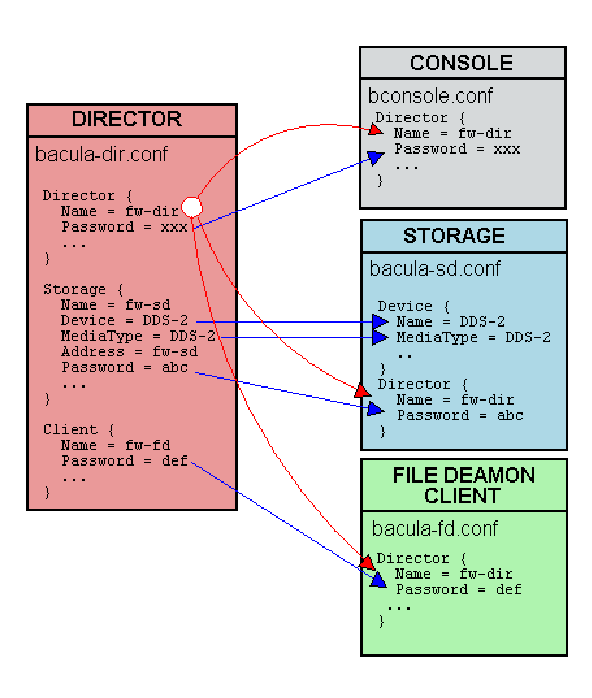
\includegraphics{./Conf-Diagram.eps}  

   In the left column, you will find the Director, Storage, and  Client
   resources, with their names and passwords -- these  are all in {\bf
   bacula-dir.conf}. In the right column  are where the corresponding values
   should be found in the  Console, Storage daemon (SD), and File daemon (FD)
   configuration  files.  

\label{AccessProblems}

\item [Bacula Runs Fine but Cannot Access a Client on a Different Machine.
   Why? ]
   \index[general]{Bacula Runs Fine but Cannot Access a Client on a Different
   Machine. Why? }
   There are several reasons why Bacula could not contact a client  on a
   different machine. They are:  

\begin{itemize}
\item It is a Windows Client, and the client died because of an  improper
   configuration file. Check that the Bacula icon is in  the system tray and the
   the menu items work. If the client has  died, the icon will disappear only
when you move the mouse over  the icon.  
\item The Client address or port is incorrect or not resolved by  DNS. See if
   you can ping the client machine using the same  address as in the Client
   record.  
\item You have a firewall, and it is blocking traffic on port  9102 between
   the Director's machine and the Clients  machine (or on port 9103 between the
   Client and the Storage daemon  machines).  
\item Your password or names are not correct in both the Director and  the
   Client machine. Try configuring everything identical to  how you run the
   client on the same machine as the Director, but  just change the Address. If
that works, make the other changes  one step at a time until it works.  
\end{itemize}

\label{startover}

\item [My Catalog is Full of Test Runs, How Can I Start Over? ]
  \index[general]{My Catalog is Full of Test Runs, How Can I Start Over? }
  If you are using MySQL do the following:

\footnotesize
\begin{verbatim}
   cd <bacula-source>/src/cats
   ./drop_mysql_tables
   ./make_mysql_tables
 
\end{verbatim}
\normalsize

If you are using SQLite, do the following:

\footnotesize
\begin{verbatim}
   Delete bacula.db from your working directory.
   cd <bacula-source>/src/cats
   ./drop_sqlite_tables
   ./make_sqlite_tables
 
\end{verbatim}
\normalsize

Then write an EOF on each tape you used with {\bf Bacula} using: 

\footnotesize
\begin{verbatim}
mt -f /dev/st0 rewind
mt -f /dev/st0 weof
\end{verbatim}
\normalsize

where you need to adjust the device name for your system.  

\label{restorehang}
\item [I Run a Restore Job and Bacula Hangs. What do I do?]
   \index[general]{I Run a Restore Job and Bacula Hangs. What do I do? }
   On Bacula version 1.25 and prior, it expects you to  have the correct tape
   mounted prior to a restore. On  Bacula version 1.26 and higher, it will ask
   you for the  tape, and if the wrong one it mounted, it will inform you.  

   If you have previously done an {\bf unmount} command, all  Storage daemon
   sessions (jobs) will be completely blocked  from using the drive unmounted, so
   be sure to do a {\bf mount}  after your unmount. If in doubt, do a second {\bf
   mount}, it  won't cause any harm.  

\label{windowstart}
\item [I Cannot Get My Windows Client to Start Automatically? ]
   \index[general]{I Cannot Get My Windows Client to Start Automatically? }
   You are probably having one of two problems: either the  Client is dying due
   to an incorrect configuration file, or  you didn't do the Installation
   commands necessary to install  it as a Windows Service.  

   For the first problem, see the next FAQ question. For the  second problem,
   please review the 
   \ilink{ Windows Installation instructions}{_ChapterStart7} in this
   manual.  

\label{windowsdie}

\item [My Windows Client Immediately Dies When I Start It ]
\index[general]{My Windows Client Immediately Dies When I Start It }
The most common problem is either that the configuration  file is not where it
expects it to be, or that there is an  error in the configuration file.  You
must have the configuration file in  {\bf
c:\textbackslash{}bacula\textbackslash{}bin\textbackslash{}bacula-fd.conf}.  

To {\bf see} what is going on when the File daemon starts  on Windows, do the
following:  

\footnotesize
\begin{verbatim}
    Start a DOS shell Window.
    cd c:\bacula\bin
    bacula-fd -d100 -c c:\bacula\bin\bacula-fd.conf
    
\end{verbatim}
\normalsize

This will cause the FD to write a file {\bf bacula.trace}  in the current
directory, which you can examine and determine  the problem.  

\label{scroll}
\item [When I Start the Console, the Error Messages Fly By. How can I see
   them? ]
   \index[general]{When I Start the Console, the Error Messages Fly By. How can I seethem? }
   Either use a shell window with a scroll bar, or use the gnome-console.  In any
   case, you probably should be logging all output to a file, and  then you can
   simply view the file using an editor or the {\bf less}  program. To log all
   output, I have the following in my Director's  Message resource definition:  

\footnotesize
\begin{verbatim}
    append = "/home/kern/bacula/bin/log" = all, !skipped
    
\end{verbatim}
\normalsize

Obviously you will want to change the filename to be appropriate  for your
system.  

\label{nobackup}
\item [I didn't realize that the backups were not working on my Windows 
   Client. What should I do? ]
\index[general]{I didn't realize that the backups were not working on my Windows
Client. What should I do? }
You should be sending yourself an email message for each job. This will  avoid
the possibility of not knowing about a failed backup. To do so  put something
like:  

\footnotesize
\begin{verbatim}
  Mail = yourname@yourdomain = all, !skipped
  
\end{verbatim}
\normalsize

in your Director's message resource. You should then receive one  email for
each Job that ran. When you are comfortable with what  is going on (it took me
9 months), you might change that to:  

\footnotesize
\begin{verbatim}
   MailOnError = yourname@yourdomain = all, !skipped
   
\end{verbatim}
\normalsize

then you only get email messages when a Job errors as is the case  for your
Windows machine.  

You should also be logging the Director's messages, please see the  previous
FAQ for how to do so.  

\label{sched}
\item [All my Jobs are scheduled for the same time. Will this cause
   problems? ]
   \index[general]{All my Jobs are scheduled for the same time. Will this cause
   problems? }
   No, not at all. Bacula will schedule all the Jobs at the same time,  but will
   run them one after another unless you have increased the number  of
   simultaneous jobs in the configuration files for the Director,  the File
   daemon, and the Storage daemon. The appropriate configuration  record is {\bf
   Maximum Concurrent Jobs = nn}. At the current time,  we recommend that you
   leave this set to {\bf 1} for the Director.  

\label{disk}
\item [Can Bacula Backup My System To Files instead of Tape? ]
   \index[general]{Can Bacula Backup My System To Files instead of Tape? }
   Yes, in principle, Bacula can backup to any storage  medium as long as you
   have correctly defined that medium in the  Storage daemon's Device resource.
   For an example of how to backup  to files, please see the  
   \ilink{Pruning Example}{PruningExample} in the  Recycling
   chapter of this manual. Also, there is a whole chapter  devoted to 
   \ilink{Backing Up to Disk}{_ChapterStart39}.  

\label{bigfiles}
\item [Can Bacula Backup and Restore Files Greater than 2 Giga bytes in
   Size?  ]
\index[general]{Can Bacula Backup and Restore Files Greater than 2 Giga bytes in
Size? }
If your operating system permits it, and you are running Bacula  version 1.26
or later, the answer is yes. To the best of our  knowledge all client system
supported by Bacula can handle  files larger than 2 Giga bytes.  

\label{cancel}
\item [I Started A Job then Decided I Really Did Not Want to Run It. Is
   there  a better way than {\bf ./bacula stop} to stop it?]
   \index[general]{I Started A Job then Decided I Really Did Not Want to
   Run It.  Is there a better way than ./bacula stop to stop it?  } Yes,
   you normally should use the Console command {\bf cancel} to cancel a Job
   that is either scheduled or running.  If the Job is scheduled, it will
   be marked for cancellation and will be canceled when it is scheduled to
   start.  If it is running, it will normally terminate after a few
   minutes.  If the Job is waiting on a tape mount, you may need to do a
   {\bf mount} command before it will be canceled.

\label{trademark}
\item [Why have You Trademarked the Name
   Bacula\raisebox{.6ex}{{\footnotesize \textsuperscript{\textregistered}}}?]
\index[general]{Why have You Trademarked the Name
Bacula\textsuperscript{\textregistered}? }
We have trademarked the name Bacula to ensure that all media  written by any
program named Bacula will always be compatible. Anyone  may use the name
Bacula, even in a derivative product as long as it  remains totally compatible
in all respects with the program defined  here.

\label{docversion}
\item [Why is Your Online Document for Version 1.35 of Bacula when the
   Currently  Release Version is 1.34?]
\index[general]{Why is Your Online Document for Version 1.35 of Bacula when the
Currently Release Version is 1.34? }
As Bacula is being developed, the document is also being enhanced, more  often
than not it has clarifications of existing features that  can be very useful
to our users, so we publish the very latest  document. Fortunately it is rare
that there are confusions with  new features.  

If you want to read a document that pertains only to a specific  version,
please use the one distributed in the source code.  

\label{sure}

\item [How Can I Be Sure that Bacula Really Saves and Restores All Files? ]
   \index[general]{How Can I Be Sure that Bacula Really Saves and Restores
   All Files?  } It is really quite simple, but took me awhile to figure
   out how to ``prove'' it.  First make a Bacula Rescue disk, see the
   \ilink{Disaster Recovery Using Bacula}{_ChapterStart38} of this manual.
   Second, you run a full backup of all your files on all partitions.
   Third, you run an Verify InitCatalog Job on the same FileSet, which
   effectively makes a record of all the files on your system.  Fourth, you
   run a Verify Catalog job and assure yourself that nothing has changed
   (well, between an InitCatalog and Catalog one doesn't expect anything).
   Then do the unthinkable, write zeros on your MBR (master boot record)
   wiping out your hard disk.  Now, restore your whole system using your
   Bacula Rescue disk and the Full backup you made, and finally re-run the
   Verify Catalog job.  You will see that with the exception of the
   directory modification and access dates and the files changed during the
   boot, your system is identical to what it was before you wiped your hard
   disk.

\label{upgrade}
\item [I did a Full backup last week, but now in running an Incremental,
   Bacula  says it did not find a FULL backup time, so it did a FULL backup. Why?]
   \index[general]{I did a Full backup last week, but now in running an
   Incremental, Bacula says it did not find a FULL backup time, so it did a
   FULL backup.  Why?  } Before doing an Incremental or a Differential
   backup, Bacula checks to see if there was a prior Full backup of the
   same Job that terminated successfully.  If so, it uses the date that
   full backup started as the time for comparing if files have changed.  If
   Bacula does not find a successfully full backup, it proceeds to do one.
   Perhaps you canceled the full backup, or it terminated in error.  In
   such cases, the full backup will not be successful.  You can check by
   entering {\bf list jobs} and look to see if there is a prior Job with
   the same Name that has Level F and JobStatus T (normal termination).

   Another reason why Bacula may not find a suitable Full backup is that
   every time you change the FileSet, Bacula will require a new Full
   backup.  This is necessary to ensure that all files are properly backed
   up in the case where you have added more files to the FileSet.
   Beginning with version 1.31, the FileSets are also dated when they are
   created, and this date is displayed with the name when you are listing
   or selecting a FileSet.  For more on backup levels see below.

\label{filenamelengths}
\item [How Can You Claim to Handle Unlimited Path and Filename Lengths
   when  All Other Programs Have Fixed Limits?]
   \index[general]{How Can You Claim to Handle Unlimited Path and Filename
   Lengths when All Other Programs Have Fixed Limits?  } Most of those
   other programs have been around for a long time, in fact since the
   beginning of Unix, which means that they were designed for rather small
   fixed length path and filename lengths.  Over the years, these
   restrictions have been relaxed allowing longer names.  Bacula on the
   other hand was designed in 2000, and so from the start, Path and
   Filenames have been keep in buffers that start at 256 bytes in length
   but can grow as needed to handle any length.  Most of the work is
   carried out by lower level routines making the coding rather easy.

\label{unique}
\item [What Is the Really Unique Feature of Bacula?   ]
   \index[general]{What Is the Really Unique Feature of Bacula?  } Well, it
   is hard to come up with unique features when backup programs for Unix
   machines have been around since the 1960s.  That said, I believe that
   Bacula is the first and only program to use a standard SQL interface to
   its catalog database.  Although this adds a bit of complexity and
   possibly overhead, it provides an amazingly rich set of features that
   are easy to program and enhance.  The current code has barely scratched
   the surface in this regard (version 1.31).

   The second feature, which gives a lot of power and flexibility to Bacula
   is the Bootstrap record definition.

   The third unique feature, which is currently (1.30) unimplemented, and
   thus can be called vaporware :-), is Base level saves.  When
   implemented, this will enormously reduce tape usage.

\label{sequence}

\item [If I Do Run Multiple Simultaneous Jobs, How Can I Force One
   Particular  Job to Run After Another Job? ]
\index[general]{If I Do Run Multiple Simultaneous Jobs, How Can I Force One
Particular Job to Run After Another Job? }
Yes, you can set Priorities on your jobs so that they  run in the order you
specify. Please see:  
\ilink{the Priority record}{Priority} in the  Job resource.

\label{nomail}

\item [I Am Not Getting Email Notification, What Can I Do?

   ]
\index[general]{I Am Not Getting Email Notification, What Can I Do? }
The most common problem is that you have not specified a fully  qualified
email address and your bsmtp server is rejecting the mail.  The next most
common problem is that your bsmtp server doesn't like  the syntax on the From
part of the message. For more details on this  and other problems, please see
the 
\ilink{ Getting Email Notification to Work}{email} section of the
Tips chapter  of this manual. The section 
\ilink{ Getting Notified of Job Completion}{notification} of the Tips
chapter may also  be useful. For more information on the {\bf bsmtp} mail
program,  please see 
\ilink{bsmtp in the Volume Utility Tools chapter}{bsmtp} of this
manual.

\label{periods}

\item [I Change Recycling, Retention Periods, or File Sizes in my Pool
   Resource  and they Still Don``t Work.]
  \index[general]{I Change Recycling, Retention Periods, or File Sizes in my Pool
  Resource and they Still Don"t Work. }
  The different variables associated with a Pool are defined in the  Pool
  Resource, but are actually read by Bacula from the Catalog database.  On
  Bacula versions prior to 1.30, after changing your Pool Resource,  you must
  manually update the corresponding values in the Catalog by  using the {\bf
  update pool} command in the Console program. In Bacula  version 1.30, Bacula
  does this for you automatically every time it  starts.  
  
  When Bacula creates a Media record (Volume), it uses many default  values from
  the Pool record. If you subsequently change the Pool  record, the new values
  will be used as a default for the next Volume  that is created, but if you
  want the new values to apply to existing  Volumes, you must manually update
  the Volume Catalog entry using  the {\bf update volume} command in the Console
  program. 

\label{CompressionNotWorking}
\item [I Have Configured Compression On, But None of My Files Are
   Compressed.  Why?]
   \index[general]{I Have Configured Compression On, But None of My Files Are
   Compressed. Why? }
   There are two kinds of compression. One is tape compression. This  is done by
   the tape drive hardware, and you either enable or disable  it with system
   tools such as {\bf mt}. This compression works  independently of Bacula.  
   
   Bacula also has compression code, which is normally used only when  backing up
   to file Volumes. There are two conditions for this  ''software`` to be
   enabled.  

\begin{enumerate}
\item You must have the zip development libraries loaded on your  system when
   building Bacula and Bacula must find this library,  normally {\bf
   /usr/lib/libz.a}. On RedHat systems, this library  is provided by the {\bf
   zlib-devel} rpm.  

 If the library is found by Bacula during the {\bf ./configure}  it will be
 in dicated on the {\bf config.out} line by:  

\footnotesize
\begin{verbatim}
             ZLIB support:  yes
          
\end{verbatim}
\normalsize

\item You must add the {\bf compression=gzip} option on your  Include
   statement in the Director's configuration file.  
\end{enumerate}

\label{NewTape}
\item [Bacula is Asking for a New Tape After 2 GB of Data but My Tape
   holds 33 GB. Why?]
\index[general]{Bacula is Asking for a New Tape After 2 GB of Data but My Tape
holds 33 GB. Why? }
There are several reasons why Bacula will request a new tape.  

\begin{itemize}
\item There is an I/O error on the tape. Bacula prints an error message  and
   requests a new tape. Bacula does not attempt to continue writing  after an I/O
   error.  
\item Bacula encounters and end of medium on the tape. This is not always 
   distinguishable from an I/O error.  
\item You have specifically set some size limitation on the tape. For  example
   the {\bf Maximum Volume Bytes} or {\bf Maximum Volume Files}  in the
   Director's Pool resource, or {\bf Maximum Volume Size} in  the Storage
  daemon's Device resource.  
\end{itemize}

\label{LevelChanging}

\item [Bacula is Not Doing the Right Thing When I Request an Incremental
   Backup. Why?]
   \index[general]{Bacula is Not Doing the Right Thing When I Request an Incremental
   Backup. Why? }
   As explained in one of the previous questions, Bacula will automatically 
   upgrade an Incremental or Differential job to a Full backup if it cannot  find
   a prior Full backup or a suitable Full backup. For the gory details  on
   how/when Bacula decides to upgrade levels please see the  
   \ilink{Level record}{Level} in the Director's  configuration
   chapter of this manual.  
   
   If after reading the above mentioned section, you believe that Bacula  is not
   correctly handling the level (Differential/Incremental),  please send us the
   following information for analysis:  

\begin{itemize}
\item Your Director's configuration file.  
\item The output from {\bf list jobs} covering the period where you  are
   having the problem.  
\item The Job report output from the prior Full save (not critical).  
\item An {\bf llist jobid=nnn} where nnn is the JobId of the prior  Full save.
 
\item The Job report output from the save that is doing the  wrong thing (not
   critical).  
\item An {\bf llist jobid=nnn} where nnn is the JobId of the job  that was not
   correct.  
\item An explanation of what job went wrong and why you think it did.  
   \end{itemize}

The above information can allow us to analyze what happened, without it, 
there is not much we can do.  

\label{WaitForever}
\item [I am Backing Up an Offsite Machine with an Unreliable Connection.
   The  Director Waits Forever for the Client to Contact the SD. What Can  I Do.]
   \index[general]{I am Backing Up an Offsite Machine with an Unreliable Connection.
   The Director Waits Forever for the Client to Contact the SD. What Can I Do. }
   Bacula was written  on the assumption that it will have a good TCP/IP
   connection  between all the daemons. As a consequence, the current  Bacula
   doesn't deal with faulty connection very well. This situation  is slowly being
   corrected over time.  
   
   There are several things you can do to improve the situation.  

\begin{itemize}
\item Upgrade to version 1.32 and use the new SDConnectTimeout record.  For
   example, set:  

\footnotesize
\begin{verbatim}
          SD Connect Timeout = 5 min
          
\end{verbatim}
\normalsize

in the FileDaemon resource.  
\item Run these kinds of jobs after all other jobs.  
   \end{itemize}

\label{sshHanging}
\item [When I ssh into a machine and start Bacula then attempt to exit, 
   ssh hangs forever.]
   \index[general]{When I ssh into a machine and start Bacula then attempt to exit,
   ssh hangs forever. }
   This happens because Bacula leaves stdin, stdout, and stderr open  for debug
   purposes. To avoid it, the simplest thing to do is to  redirect the output of
   those files to {\bf /dev/null} or another  file in your startup script (the
   RedHat autostart scripts do this  automatically). For example, you start the
   Director with:  
   
\footnotesize
\begin{verbatim}
    bacula-dir -c bacula-dir.conf ... 0>\&1 2>\&1 >/dev/null
    
\end{verbatim}
\normalsize

and likewise for the other daemons.  

\label{RetentionPeriods}

\item [I'm confused by the different Retention periods: File Retention, 
   Job Retention, Volume Retention. Why are there so many?]
   \index[general]{I'm confused by the different Retention periods: File Retention,
   Job Retention, Volume Retention. Why are there so many? }
   Yes, this certainly can be confusing. The basic reason for so many  is to
   allow flexibility. The File records take quite a lot of space  in the catalog,
   so they are typically records you want to remove  rather quickly. The Job
   records, take very little space, and they  can be useful even without the File
   records to see what Jobs actually  ran and when. One must understand that if
   the File records are removed  from the catalog, you cannot use the {\bf
   restore} command to restore  an individual file since Bacula no longer knows
   where it is. However,  as long as the Volume Retention period has not expired,
   the data will  still be on the tape, and can be recovered from the tape.  
   
   For example, I keep a 30 day retention period for my Files to  keep my catalog
   from getting too big, but I keep my tapes for a  minimum of one year, just in
   case.  

\label{MaxVolumeSize}
\item [Why Does Bacula Ignore the MaxVolumeSize Set in my Pool?]
   \index[general]{Why Does Bacula Ignore the MaxVolumeSize Set in my Pool? }
   The MaxVolumeSize that Bacula uses comes from the Media record,  so most
   likely you changed your Pool, which is used as the default  for creating Media
   records, {\bf after} you created your Volume. Check  what is in the Media
   record by doing: 

\footnotesize
\begin{verbatim}
llist Volume=xxx
\end{verbatim}
\normalsize

If it doesn't have the right value, you can use: 

\footnotesize
\begin{verbatim}
update Volume=xxx
\end{verbatim}
\normalsize

to change it.  

\label{ConnectionRefused}
\item [In connecting to my Client, I get ''ERR:Connection Refused.  Packet
   Size too big from File daemon:192.168.1.4:9102`` Why?]
   \index[general]{In connecting to my Client, I get &htmlQuoteERR:Connection Refused.
   Packet Size too big from File daemon:192.168.1.4:9102&htmlQuote Why? }
   This is typically a communications error resulting  from one of the following:
 

\begin{itemize}
\item Old versions of Bacula, usually a Win32 client, where two  threads were
   using the same I/O packet. Fixed in more recent  versions. Please upgrade.  
\item Some other program such as an HP Printer using the same  port (9102 in
   this case).  
\end{itemize}

If it is neither of the above, please submit a bug report at  
\elink{bugs.bacula.org}{http://bugs.bacula.org}.  

Another solution might be to run the daemon with the debug  option by:  

\footnotesize
\begin{verbatim}
    Start a DOS shell Window.
    cd c:\bacula\bin
    bacula-fd -d100 -c c:\bacula\bin\bacula-fd.conf
    
\end{verbatim}
\normalsize

This will cause the FD to write a file {\bf bacula.trace}  in the current
directory, which you can examine and determine  the problem.  

\end{description}

%%
%%

\section*{Tips and Suggestions}
\label{_ChapterStart8}
\index[general]{Tips and Suggestions }
\index[general]{Suggestions!Tips and }
\addcontentsline{toc}{section}{Tips and Suggestions}

\subsection*{Examples}
\label{examples}
\index[general]{Examples }
\addcontentsline{toc}{subsection}{Examples}

There are a number of example scripts for various things that can be found in
the {\bf example} subdirectory and its subdirectories of the Bacula source
distribution. 

\subsection*{Upgrading Bacula Versions}
\label{upgrading}
\index[general]{Upgrading Bacula Versions }
\index[general]{Versions!Upgrading Bacula }
\addcontentsline{toc}{subsection}{Upgrading Bacula Versions}

The first thing to do before upgrading from one version to another is to
ensure that don't overwrite or delete your production (current) version of Bacula until
you have tested that the new version works. 

If you have installed Bacula into a single directory, this is simple: simply
make a copy of your Bacula directory. 

If you have done a more typical Unix installation where the binaries are
placed in one directory and the configuration files are placed in another,
then the simplest way is to configure your new Bacula to go into a single
file. Alternatively, make copies of all your binaries and especially your 
conf files.

Whatever your situation may be (one of the two just described), you should
probably start with the {\bf defaultconf} script that can be found in the {\bf
examples} subdirectory. Copy this script to the main Bacula directory, modify
it as necessary (there should not need to be many modifications), configure
Bacula, build it, install it, then stop your production Bacula, copy all the
{\bf *.conf} files from your production Bacula directory to the test Bacula
directory, start the test version, and run a few test backups. If all seems
good, then you can proceed to install the new Bacula in place of or possibly
over the old Bacula. 

When installing a new Bacula you need not worry about losing the changes you
made to your configuration files as the installation process will not
overwrite them providing that you do not do a {\bf make uninstall}.

\subsection*{Getting Notified of Job Completion}
\label{notification}
\index[general]{Getting Notified of Job Completion }
\index[general]{Completion!Getting Notified of Job }
\addcontentsline{toc}{subsection}{Getting Notified of Job Completion}

One of the first things you should do is to ensure that you are being properly
notified of the status of each Job run by Bacula, or at a minimum of each Job
that terminates with an error. 

Until you are completely comfortable with {\bf Bacula}, we recommend that you
send an email to yourself for each Job that is run. This is most easily
accomplished by adding an email notification address in the {\bf Messages}
resource of your Director's configuration file. An email is automatically
configured in the default configuration files, but you must ensure that the
default {\bf root} address is replaced by your email address. 

For examples of how I (Kern) configure my system, please take a look at the
{\bf .conf} files found in the {\bf examples} sub-directory. We recommend the
following configuration (where you change the paths and email address to
correspond to your setup). Note, the {\bf mailcommand} and {\bf
operatorcommand} should be on a single line. They were split here for
presentation: 

\footnotesize
\begin{verbatim}
Messages {
  Name = Standard
  mailcommand = "/home/bacula/bin/bsmtp -h localhost
                -f \"\(Bacula\) %r\"
                -s \"Bacula: %t %e of %c %l\" %r"
  operatorcommand = "/home/bacula/bin/bsmtp -h localhost
                -f \"\(Bacula\) %r\"
                -s \"Bacula: Intervention needed for %j\" %r"
  Mail = your-email-address = all, !skipped, !terminate
  append = "/home/bacula/bin/log" = all, !skipped, !terminate
  operator = your-email-address = mount
  console = all, !skipped, !saved
}
\end{verbatim}
\normalsize

You will need to ensure that the {\bf /home/bacula/bin} path on the {\bf
mailcommand} and the {\bf operatorcommand} lines points to your {\bf Bacula}
binary directory where the {\bf bsmtp} program will be installed. You will
also want to ensure that the {\bf your-email-address} is replaced by your
email address, and finally, you will also need to ensure that the {\bf
/home/bacula/bin/log} points to the file where you want to log all messages. 

With the above Messages resource, you will be notified by email of every Job
that ran, all the output will be appended to the {\bf log} file you specify,
all output will be directed to the console program, and all mount messages
will be emailed to you. Note, some messages will be sent to multiple
destinations. 

The form of the mailcommand is a bit complicated, but it allows you to
distinguish whether the Job terminated in error or terminated normally. Please
see the 
\ilink{Mail Command}{mailcommand} section of the Messages
Resource chapter of this manual for the details of the substitution characters
used above. 

Once you are totally comfortable with Bacula as I am, or if you have a large
number of nightly Jobs as I do (eight), you will probably want to change the
{\bf Mail} command to {\bf Mail On Error} which will generate an email message
only if the Job terminates in error. If the Job terminates normally, no email
message will be sent, but the output will still be appended to the log file as
well as sent to the Console program. 

\subsection*{Getting Email Notification to Work}
\label{email}
\index[general]{Work!Getting Email Notification to }
\index[general]{Getting Email Notification to Work }
\addcontentsline{toc}{subsection}{Getting Email Notification to Work}

The section above describes how to get email notification of job status.
Occasionally, however, users have problems receiving any email at all. In that
case, the things to check are the following: 

\begin{itemize}
\item Ensure that you have a valid email address specified on your  {\bf Mail}
   record in the Director's Messages resource. The email  address should be fully
   qualified. Simply using {\bf root} generally  will not work, rather you should
use {\bf root@localhost} or better  yet your full domain.  
\item Ensure that you do not have a {\bf Mail} record in the Storage  daemon's
   or File daemon's configuration files. The only record  you should have is {\bf
   director}:  

\footnotesize
\begin{verbatim}
      director = director-name = all
      
\end{verbatim}
\normalsize

\item If all else fails, try replacing the {\bf mailcommand} with 

   \footnotesize
\begin{verbatim}
mailcommand = "mail -s test your@domain.com"
\end{verbatim}
\normalsize

\item Once the above is working, assuming you want to use {\bf bsmtp},  submit
   the desired bsmtp command by hand and ensure that the email  is delivered,
   then put that command into {\bf Bacula}. Small  differences in things such as
the parenthesis around the word  Bacula can make a big difference to some
bsmtp programs.  For example, you might start simply by using: 

\footnotesize
\begin{verbatim}
mailcommand = "/home/bacula/bin/bsmtp -f \"root@localhost\" %r"
\end{verbatim}
\normalsize

\end{itemize}

\subsection*{Getting Notified that Bacula is Running}
\label{JobNotification}
\index[general]{Running!Getting Notified that Bacula is }
\index[general]{Getting Notified that Bacula is Running }
\addcontentsline{toc}{subsection}{Getting Notified that Bacula is Running}

If like me, you have setup Bacula so that email is sent only when a Job has
errors, as described in the previous section of this chapter, inevitably, one
day, something will go wrong and {\bf Bacula} can stall. This could be because
Bacula crashes, which is vary rare, or more likely the network has caused {\bf
Bacula} to {\bf hang} for some unknown reason. 

To avoid this, you can use the {\bf RunAfterJob} command in the Job resource
to schedule a Job nightly, or weekly that simply emails you a message saying
that Bacula is still running. For example, I have setup the following Job in
my Director's configuration file: 

\footnotesize
\begin{verbatim}
Schedule {
  Name = "Watchdog"
  Run = Level=Full sun-sat at 6:05
}
Job {
  Name = "Watchdog"
  Type = Admin
  Client=Watchdog
  FileSet="Verify Set"
  Messages = Standard
  Storage = DLTDrive
  Pool = Default
  Schedule = "Watchdog"
  RunAfterJob = "/home/kern/bacula/bin/watchdog %c %d"
}
Client {
  Name = Watchdog
  Address = rufus
  FDPort = 9102
  Catalog = Verify
  Password = ""
  File Retention = 1day
  Job Retention = 1 month
  AutoPrune = yes
}
\end{verbatim}
\normalsize

Where I established a schedule to run the Job nightly. The Job itself is type
{\bf Admin} which means that it doesn't actually do anything, and I've defined
a FileSet, Pool, Storage, and Client, all of which are not really used (and
probably don't need to be specified). The key aspect of this Job is the
command: 

\footnotesize
\begin{verbatim}
  RunAfterJob = "/home/kern/bacula/bin/watchdog %c %d"
\end{verbatim}
\normalsize

which runs my ``watchdog'' script. As an example, I have added the Job codes
\%c and \%d which will cause the Client name and the Director's name to be
passed to the script. For example, if the Client's name is {\bf Watchdog} and
the Director's name is {\bf main-dir} then referencing \$1 in the script would
get {\bf Watchdog} and referencing \$2 would get {\bf main-dir}. In this case,
having the script know the Client and Director's name is not really useful,
but in other situations it may be. 

You can put anything in the watchdog scrip. In my case, I like to monitor the
size of my catalog to be sure that {\bf Bacula} is really pruning it. The
following is my watchdog script: 

\footnotesize
\begin{verbatim}
#!/bin/sh
cd /home/kern/mysql/var/bacula
du . * |
/home/kern/bacula/bin/bsmtp  \
   -f "\(Bacula\) abuse@whitehouse.com" -h mail.yyyy.com \
   -s "Bacula running" abuse@whitehouse.com
\end{verbatim}
\normalsize

If you just wish to send yourself a message, you can do it with: 

\footnotesize
\begin{verbatim}
#!/bin/sh
cd /home/kern/mysql/var/bacula
/home/kern/bacula/bin/bsmtp  \
   -f "\(Bacula\) abuse@whitehouse.com" -h mail.yyyy.com \
   -s "Bacula running" abuse@whitehouse.com <<END-OF-DATA
Bacula is still running!!!
END-OF-DATA
\end{verbatim}
\normalsize

\subsection*{Maintaining a Valid Bootstrap File}
\label{bootstrap}
\index[general]{Maintaining a Valid Bootstrap File }
\index[general]{File!Maintaining a Valid Bootstrap }
\addcontentsline{toc}{subsection}{Maintaining a Valid Bootstrap File}

By using a 
\ilink{ WriteBootstrap}{writebootstrap} record in each of your
Director's Job resources, you can constantly maintain a 
\ilink{bootstrap}{_ChapterStart43} file that will enable you to
recover the state of your system as of the last backup without having the
Bacula catalog. This permits you to more easily recover from a disaster that
destroys your Bacula catalog. 

When a Job resource has a {\bf WriteBootstrap} record, Bacula will maintain
the designated file (normally on another system but mounted by NSF) with up to
date information necessary to restore your system. For example, in my
Director's configuration file, I have the following record: 

\footnotesize
\begin{verbatim}
 Write Bootstrap = "/mnt/deuter/files/backup/client-name.bsr"
\end{verbatim}
\normalsize

where I replace {\bf client-name} by the actual name of the client that is
being backed up. Thus, Bacula automatically maintains one file for each of my
clients. The necessary bootstrap information is appended to this file during
each {\bf Incremental} backup, and the file is totally rewritten during each
{\bf Full} backup. 

Note, one major disadvantage of writing to an NFS mounted volume as I do is
that if the other machine goes down, the OS will wait forever on the fopen()
call that Bacula makes. As a consequence, Bacula will completely stall until
the machine exporting the NSF mounts comes back up. The solution to this
problem was provided by Andrew Hilborne, and consists of using the {\bf soft}
option instead of the {\bf hard} option when mounting the NFS volume, which is
typically done in {\bf /etc/fstab}/. The NFS documentation explains these
options in detail. 

If you are starting off in the middle of a cycle (i.e. with Incremental
backups) rather than at the beginning (with a Full backup), the {\bf
bootstrap} file will not be immediately valid as it must always have the
information from a Full backup as the first record. If you wish to synchronize
your bootstrap file immediately, you can do so by running a {\bf restore}
command for the client and selecting a full restore, but when the restore
command asks for confirmation to run the restore Job, you simply reply no,
then copy the bootstrap file that was written to the location specified on the
{\bf Write Bootstrap} record. The restore bootstrap file can be found in {\bf
restore.bsr} in the working directory that you defined. In the example given
below for the client {\bf rufus}, my input is shown in bold. Note, the JobId
output has been partially truncated to fit on the page here: 

\footnotesize
\begin{verbatim}
(in the Console program)
*{\bf restore}
First you select one or more JobIds that contain files
to be restored. You will then be presented several methods
of specifying the JobIds. Then you will be allowed to
select which files from those JobIds are to be restored.
To select the JobIds, you have the following choices:
     1: List last 20 Jobs run
     2: List Jobs where a given File is saved
     3: Enter list of JobIds to select
     4: Enter SQL list command
     5: Select the most recent backup for a client
     6: Cancel
Select item:  (1-6): {\bf 5}
The defined Client resources are:
     1: Minimatou
     2: Rufus
     3: Timmy
Select Client (File daemon) resource (1-3): {\bf 2}
The defined FileSet resources are:
     1: Kerns Files
Item 1 selected automatically.
+-------+------+-------+---------+---------+------+-------+------------+
| JobId | Levl | Files | StrtTim | VolName | File | SesId | VolSesTime |
+-------+------+-------+---------+---------+------+-------+------------+
| 2     | F    | 84    |  ...    | test1   | 0    | 1     | 1035645259 |
+-------+------+-------+---------+---------+------+-------+------------+
You have selected the following JobId: 2
Building directory tree for JobId 2 ...
The defined Storage resources are:
     1: File
Item 1 selected automatically.
You are now entering file selection mode where you add and
remove files to be restored. All files are initially added.
Enter "done" to leave this mode.
cwd is: /
$ {\bf done}
84 files selected to restore.
Run Restore job
JobName:    kernsrestore
Bootstrap:  /home/kern/bacula/working/restore.bsr
Where:      /tmp/bacula-restores
FileSet:    Kerns Files
Client:     Rufus
Storage:    File
JobId:      *None*
OK to run? (yes/mod/no): {\bf no}
{\bf quit}
(in a shell window)
{\bf cp ../working/restore.bsr /mnt/deuter/files/backup/rufus.bsr}
\end{verbatim}
\normalsize

\subsection*{Rejected Volumes After a Crash}
\label{RejectedVolumes}
\index[general]{Crash!Rejected Volumes After a }
\index[general]{Rejected Volumes After a Crash }
\addcontentsline{toc}{subsection}{Rejected Volumes After a Crash}

Bacula keeps a count of the number of files on each Volume in its Catalog
database so that before appending to a tape, it can verify that the number of
files are correct, and thus prevent overwriting valid data. If the Director or
the Storage daemon crashes before the job has completed, the tape will contain
one more file than is noted in the Catalog, and the next time you attempt to
use the same Volume, Bacula will reject it due to a mismatch between the
physical tape (Volume) and the catalog. 

The easiest solution to this problem is to label a new tape and start fresh.
If you wish to continue appending to the current tape, you can do so by using
the {\bf update} command in the console program to change the {\bf Volume
Files} entry in the catalog. A typical sequence of events would go like the
following: 

\footnotesize
\begin{verbatim}
- Bacula crashes
- You restart Bacula
\end{verbatim}
\normalsize

Bacula then prints: 

\footnotesize
\begin{verbatim}
17-Jan-2003 16:45 rufus-dir: Start Backup JobId 13,
                  Job=kernsave.2003-01-17_16.45.46
17-Jan-2003 16:45 rufus-sd: Volume test01 previously written,
                  moving to end of data.
17-Jan-2003 16:46 rufus-sd: kernsave.2003-01-17_16.45.46 Error:
                  I cannot write on this volume because:
                  The number of files mismatch! Volume=11 Catalog=10
17-Jan-2003 16:46 rufus-sd: Job kernsave.2003-01-17_16.45.46 waiting.
                   Cannot find any appendable volumes.
Please use the "label"  command to create a new Volume for:
    Storage:      SDT-10000
    Media type:   DDS-4
    Pool:         Default
\end{verbatim}
\normalsize

(note, lines wrapped for presentation)
The key here is the line that reads: 

\footnotesize
\begin{verbatim}
  The number of files mismatch! Volume=11 Catalog=10
\end{verbatim}
\normalsize

It says that Bacula found eleven files on the volume, but that the catalog
says there should be ten. When you see this, you can be reasonably sure that
the SD was interrupted while writing before it had a chance to update the
catalog. As a consequence, you can just modify the catalog count to eleven,
and even if the catalog contains references to files saved in file 11,
everything will be OK and nothing will be lost. Note that if the SD had
written several file marks to the volume, the difference between the Volume
cound and the Catalog count could be larger than one, but this is unusual. 

If on the other hand the catalog is marked as having more files than Bacula
found on the tape, you need to consider the possible negative consequences of
modifying the catalog. Please see below for a more complete discussion of
this. 

Continuing with the example of {\bf Volume = 11 Catalog = 10}, to enable to
Bacula to append to the tape, you do the following: 

\footnotesize
\begin{verbatim}
{\bf update}
Update choice:
     1: Volume parameters
     2: Pool from resource
     3: Slots from autochanger
Choose catalog item to update (1-3): {\bf 1}
Defined Pools:
     1: Default
     2: File
Select the Pool (1-2):
+-------+---------+--------+---------+-----------+------+----------+------+-----+
| MedId | VolName | MedTyp | VolStat | VolBytes  | Last | VolReten | Recy | Slt |
+-------+---------+--------+---------+-----------+------+----------+------+-----+
| 1     | test01  | DDS-4  | Error   | 352427156 | ...  | 31536000 | 1    | 0   |
+-------+---------+--------+---------+-----------+------+----------+------+-----+
Enter MediaId or Volume name: {\bf 1}
\end{verbatim}
\normalsize

(note table output truncated for presentation) First, you chose to update the
Volume parameters by entering a {\bf 1}. In the volume listing that follows,
notice how the VolStatus is {\bf Error}. We will correct that after changing
the Volume Files. Continuing, you respond 1, 

\footnotesize
\begin{verbatim}
Updating Volume "test01"
Parameters to modify:
     1: Volume Status
     2: Volume Retention Period
     3: Volume Use Duration
     4: Maximum Volume Jobs
     5: Maximum Volume Files
     6: Maximum Volume Bytes
     7: Recycle Flag
     8: Slot
     9: Volume Files
    10: Pool
    11: Done
Select parameter to modify (1-11): {\bf 9}
Warning changing Volume Files can result
in loss of data on your Volume
Current Volume Files is: 10
Enter new number of Files for Volume: {\bf 11}
New Volume Files is: 11
Updating Volume "test01"
Parameters to modify:
     1: Volume Status
     2: Volume Retention Period
     3: Volume Use Duration
     4: Maximum Volume Jobs
     5: Maximum Volume Files
     6: Maximum Volume Bytes
     7: Recycle Flag
     8: Slot
     9: Volume Files
    10: Pool
    11: Done
Select parameter to modify (1-10): {\bf 1}
\end{verbatim}
\normalsize

Here, you have selected {\bf 9} in order to update the Volume Files, then you
changed it from {\bf 10} to {\bf 11}, and you now answer {\bf 1} to change the
Volume Status. 

\footnotesize
\begin{verbatim}
Current Volume status is: Error
Possible Values are:
     1: Append
     2: Archive
     3: Disabled
     4: Full
     5: Used
     6: Read-Only
Choose new Volume Status (1-6): {\bf 1}
New Volume status is: Append
Updating Volume "test01"
Parameters to modify:
     1: Volume Status
     2: Volume Retention Period
     3: Volume Use Duration
     4: Maximum Volume Jobs
     5: Maximum Volume Files
     6: Maximum Volume Bytes
     7: Recycle Flag
     8: Slot
     9: Volume Files
    10: Pool
    11: Done
Select parameter to modify (1-11): {\bf 11}
Selection done.
\end{verbatim}
\normalsize

At this point, you have changed the Volume Files from {\bf 10} to {\bf 11} to
account for the last file that was written but not updated in the database,
and you changed the Volume Status back to {\bf Append}. 

This was a lot of words to describe something quite simple. 

The {\bf Volume Files} option exists only in version 1.29 and later, and you
should be careful using it. Generally, if you set the value to that which
Bacula said is on the tape, you will be OK, especially if the value is one
more than what is in the catalog. 

Now lets consider the case: 

\footnotesize
\begin{verbatim}
  The number of files mismatch! Volume=10 Catalog=12
\end{verbatim}
\normalsize

Here the Bacula found fewer files on the volume than what is marked in the
catalog. Now, in this case, you should hesitate lot before modifying the count
in the catalog, because if you force the catalog from 12 to 10, Bacula will
start writing after the file 10 on the tape, possibly overwriting valid data,
and if you ever try to restore any of the files that the catalog has marked as
saved on Files 11 and 12, all chaos will break out. In this case, you will
probably be better off using a new tape. In fact, you might want to see what
files the catalog claims are actually stored on that Volume, and back them up
to another tape and recycle this tape. 

\subsection*{Security Considerations}
\label{security}
\index[general]{Considerations!Security }
\index[general]{Security Considerations }
\addcontentsline{toc}{subsection}{Security Considerations}

Only the File daemon needs to run with root permission (so that it can access
all files). As a consequence, you may run your Director, Storage daemon, and
MySQL or PostgreSQL database server as non-root processes. Version 1.30 has
the {\bf -u} and the {\bf -g} options that allow you to specify a userid and
groupid on the command line to be used after Bacula starts. 

As of version 1.33, thanks to Dan Langille, it is easier to configure the
Bacula Director and Storage daemon to run as non-root. 

You should protect the Bacula port addresses (normally 9101, 9102, and 9103)
from outside access by a firewall or other means of protection to prevent
unauthorized use of your daemons. 

You should ensure that the configuration files are not world readable since
they contain passwords that allow access to the daemons. Anyone who can access
the Director using a console program can restore any file from a backup
Volume. 

You should protect your Catalog database. If you are using SQLite, make sure
that the working directory is readable only by root (or your Bacula userid),
and ensure that {\bf bacula.db} has permissions {\bf -rw-r\verb{--{r\verb{--{} (i.e. 640) or
more strict. If you are using MySQL or PostgreSQL, please note that the Bacula
setup procedure leaves the database open to anyone. At a minimum, you should
assign the user {\bf bacula} a userid and add it to your Director's
configuration file in the appropriate Catalog resource. 

\subsection*{Creating Holiday Schedules}
\label{holiday}
\index[general]{Schedules!Creating Holiday }
\index[general]{Creating Holiday Schedules }
\addcontentsline{toc}{subsection}{Creating Holiday Schedules}

If you normally change tapes every day or at least every Friday, but Thursday
is a holiday, you can use a trick proposed by Lutz Kittler to ensure that no
job runs on Thursday so that you can insert Friday's tape and be sure it will
be used on Friday. To do so, define a {\bf RunJobBefore} script that normally
returns zero, so that the Bacula job will normally continue. You can then
modify the script to return non-zero on any day when you do not want Bacula to
run the job. 

\subsection*{Automatic Labeling Using Your Autochanger}
\label{autolabel}
\index[general]{Automatic Labeling Using Your Autochanger }
\index[general]{Autochanger!Automatic Labeling Using Your }
\addcontentsline{toc}{subsection}{Automatic Labeling Using Your Autochanger}

If you have an autochanger but it does not support barcodes, using a ``trick''
you can make Bacula automatically label all the volumes in your autochanger's
magazine. 

First create a file containing one line for each slot in your autochanger that
has a tape to be labeled. The line will contain the slot number a colon (:)
then the Volume name you want to use. For example, create a file named {\bf
volume-list}, which contains: 

\footnotesize
\begin{verbatim}
1:Volume001
2:TestVolume02
5:LastVolume
\end{verbatim}
\normalsize

The records do not need to be in any order and you don't need to mention all
the slots. Normally, you will have a consistent set of Volume names and a
sequential set of numbers for each slot you want labeled. In the example
above, I've left out slots 3 and 4 just as an example. Now, modify your {\bf
mtx-changer} script and comment out all the lines in the {\bf list)} case by
putting a \# in column 1. Then add the following two lines: 

\footnotesize
\begin{verbatim}
  cat <absolute-path>/volume-list
  exit 0
\end{verbatim}
\normalsize

so that the whole case looks like: 

\footnotesize
\begin{verbatim}
  list)
#
# commented out lines
   cat <absolute-path>/volume-list
   exit 0
   ;;
\end{verbatim}
\normalsize

where you replace \lt{}absolute-path\gt{} with the full path to the
volume-list file. Then using the console, you enter the following command: 

\footnotesize
\begin{verbatim}
   label barcodes
\end{verbatim}
\normalsize

and Bacula will proceed to mount the autochanger Volumes in the list and label
them with the Volume names you have supplied. Bacula will think that the list
was provided by the autochanger barcodes, but in reality, it was you who
supplied the \lt{}barcodes\gt{}. 

If it seems to work, when it finishes, enter: 

\footnotesize
\begin{verbatim}
   list volumes
\end{verbatim}
\normalsize

and you should see all the volumes nicely created. 

\subsection*{Backing Up Portables Using DHCP}
\label{DNS}
\index[general]{DHCP!Backing Up Portables Using }
\index[general]{Backing Up Portables Using DHCP }
\addcontentsline{toc}{subsection}{Backing Up Portables Using DHCP}

You may want to backup laptops or portables that are not always connected to
the network. If you are using DHCP to assign an IP address to those machines
when they connect, you will need to use the Dynamic Update capability of DNS
to assign a name to those machines that can be used in the Address field of
the Client resource in the Director's conf file. 

\subsection*{Going on Vacation}
\label{Vacation}
\index[general]{Vacation!Going on }
\index[general]{Going on Vacation }
\addcontentsline{toc}{subsection}{Going on Vacation}

At some point, you may want to be absent for a week or two and you want to
make sure Bacula has enough tape left so that the backups will complete. You
start by doing a {\bf list volumes} in the Console program: 

\footnotesize
\begin{verbatim}
{\bf list volumes}
 
Using default Catalog name=BackupDB DB=bacula
Pool: Default
+---------+---------------+-----------+-----------+----------------+-
| MediaId | VolumeName    | MediaType | VolStatus |       VolBytes |
+---------+---------------+-----------+-----------+----------------+-
|      23 | DLT-30Nov02   | DLT8000   | Full      | 54,739,278,128 |
|      24 | DLT-21Dec02   | DLT8000   | Full      | 56,331,524,629 |
|      25 | DLT-11Jan03   | DLT8000   | Full      | 67,863,514,895 |
|      26 | DLT-02Feb03   | DLT8000   | Full      | 63,439,314,216 |
|      27 | DLT-03Mar03   | DLT8000   | Full      | 66,022,754,598 |
|      28 | DLT-04Apr03   | DLT8000   | Full      | 60,792,559,924 |
|      29 | DLT-28Apr03   | DLT8000   | Full      | 62,072,494,063 |
|      30 | DLT-17May03   | DLT8000   | Full      | 65,901,767,839 |
|      31 | DLT-07Jun03   | DLT8000   | Used      | 56,558,490,015 |
|      32 | DLT-28Jun03   | DLT8000   | Full      | 64,274,871,265 |
|      33 | DLT-19Jul03   | DLT8000   | Full      | 64,648,749,480 |
|      34 | DLT-08Aug03   | DLT8000   | Full      | 64,293,941,255 |
|      35 | DLT-24Aug03   | DLT8000   | Append    |  9,999,216,782 |
+---------+---------------+-----------+-----------+----------------+
\end{verbatim}
\normalsize

Note, I have truncated the output for presentation purposes. What is
significant for is that I can see that my current tape has almost 10 Gbytes of
data, and that the average amount of data I get on my tapes is about 60
Gbytes. So if I go on vacation now, I don't need to worry about tape capacity
(at least not for short absences). 

Equally significant is the fact that I did go on vacation the 28th of June
2003, and when I did the {\bf list volumes} command, my current tape at that
time, DLT-07Jun03 MediaId 31, had 56.5 Gbytes written. I could see that the
tape would fill shortly. Consequently, I manually marked it as {\bf Used} and
replaced it with a fresh tape that I labeled as DLT-28Jun03, thus assuring
myself that the backups would all complete without my intervention. 

\subsection*{How to Excude File on Windows Regardless of Case}
\label{Case}
\index[general]{How to Excude File on Windows Regardless of Case }
\index[general]{Case!How to Excude File on Windows Regardless of }
\addcontentsline{toc}{subsection}{How to Excude File on Windows Regardless of
Case}

This tip was submitted by Marc Brueckner who wasn't sure of the case of some
of his files on Win32, which is case insensitive. The problem is that Bacula
thinks that {\bf /UNIMPORTANT FILES} is different from {\bf /Unimportant
Files}. Marc was aware that the file exclusion permits wild-cards. So, he
specified: 

\footnotesize
\begin{verbatim}
"/[Uu][Nn][Ii][Mm][Pp][Oo][Rr][Tt][Aa][Nn][Tt] [Ff][Ii][Ll][Ee][Ss]"
\end{verbatim}
\normalsize

As a consequence, the above exclude works for files of any case. 

Please note that this works only in Bacula Exclude statement and not in
Include. 

\subsection*{Executing Scripts on a Remote Machine}
\label{RemoteExecution}
\index[general]{Machine!Executing Scripts on a Remote }
\index[general]{Executing Scripts on a Remote Machine }
\addcontentsline{toc}{subsection}{Executing Scripts on a Remote Machine}

This tip also comes from Marc Brueckner. (Note, this tip is probably outdated
by the addition of {\bf ClientRunBeforJob} and {\bf ClientRunAfterJob} Job
records, but the technique still could be useful.) First I thought the ``Run
Before Job'' statement in the Job-resource is for executing a script on the
remote machine(the machine to be backed up). It could be usefull to execute
scripts on the remote machine e.g. for stopping databases or other services
while doing the backup. (Of cause I have to start the services again when the
backup has finished) I found the following solution: Bacula could execute
scrips on the remote machine by using ssh. The authentication is done
automatically using a private key. First You have to generate a keypair. I ve
done this by: 

\footnotesize
\begin{verbatim}
ssh-keygen -b 4096 -t dsa -f Bacula_key
\end{verbatim}
\normalsize

This statement may take a little time to run. It creates a public/private key
pair with no pass phrase. You could save the keys in /etc/bacula. Now you have
two new files : Bacula\_key which contains the private key and Bacula\_key.pub
which contains the public key. 

Now you have to append the Bacula\_key.pub file to the file authorized\_keys
in the \textbackslash{}root\textbackslash{}.ssh directory of the remote
machine. Then you have to add (or uncomment) the line 

\footnotesize
\begin{verbatim}
AuthorizedKeysFile           %h/.ssh/authorized_keys
\end{verbatim}
\normalsize

to the sshd\_config file on the remote machine. Where the \%h stands for the
home-directory of the user (root in this case). 

Assuming that your sshd is already running on the remote machine, you can now
enter the folloing on the machine where Bacula runs: 

\footnotesize
\begin{verbatim}
ssh -i Bacula_key  -l root "ls -la"
\end{verbatim}
\normalsize

This should execute the ``ls -la'' command on the remote machine. 

Now you could add lines like the following to your Director's conf file: 

\footnotesize
\begin{verbatim}
...
Run Before Job = ssh -i /etc/bacula/Bacula_key 192.168.1.1 \
                 "/etc/init.d/database stop"
Run After Job = ssh -i /etc/bacula/Bacula_key 192.168.1.1 \
                 "/etc/init.d/database start"
...
\end{verbatim}
\normalsize

Even though Bacula version 1.32 has a ClientRunBeforeJob, the ssh method still
could be useful for updating all the Bacula clients on several remote machines
in a single script. 

\subsection*{Recycling All Your Volumes}
\label{recycle}
\index[general]{Recycling All Your Volumes }
\index[general]{Volumes!Recycling All Your }
\addcontentsline{toc}{subsection}{Recycling All Your Volumes}

This tip comes from Phil Stracchino. 

If you decide to blow away your catalog and start over, the simplest way to
re-add all your prelabelled tapes with the minimum of fuss (provided you don't
care about the data on the tapes) is to add the tape labels using the console
{\bf add} command, then go into the catalog and manually set the VolStatus of
every tape to {\bf Recycle}. 

The SQL command to do this is very simple: 

\footnotesize
\begin{verbatim}
update Media set VolStatus = "Recycle";
\end{verbatim}
\normalsize

Bacula will then ignore the data already stored on the tapes and just re-use
each tape without further objection. 

\subsection*{Backing up ACLs on ext3 or XFS filesystems}
\label{ACLs}
\index[general]{Filesystems!Backing up ACLs on ext3 or XFS }
\index[general]{Backing up ACLs on ext3 or XFS filesystems }
\addcontentsline{toc}{subsection}{Backing up ACLs on ext3 or XFS filesystems}

This tip comes from Volker Sauer. 

Note, this tip was given prior to implementation of ACLs in Bacula (version
1.34.5). It is left here because dumping/displaying ACLs can still be useful
in testing/verifying that Bacula is backing up and restoring your ACLs
properly. Please see the 
\ilink{aclsupport}{ACLSupport} FileSet option in the
configuration chapter of this manual. 

For example, you could dump the ACLs to a file with a script similar to the
following: 

\footnotesize
\begin{verbatim}
#!/bin/sh
BACKUP_DIRS="/foo /bar"
STORE_ACL=/root/acl-backup
umask 077
for i in $BACKUP_DIRS; do
 cd $i /usr/bin/getfacl -R --skip-base .>$STORE_ACL/${i//\//_}
done
\end{verbatim}
\normalsize

Then use Bacula to backup {\bf /root/acl-backup}. 

The ACLs could be restored using Bacula to the {\bf /root/acl-backup} file,
then restored to your system using: 

\footnotesize
\begin{verbatim}
setfacl --restore/root/acl-backup
\end{verbatim}
\normalsize

\subsection*{Total Automation of Bacula Tape Handling}
\label{automate}
\index[general]{Handling!Total Automation of Bacula Tape }
\index[general]{Total Automation of Bacula Tape Handling }
\addcontentsline{toc}{subsection}{Total Automation of Bacula Tape Handling}

This tip was provided by Alexander Kuehn. 

\elink{Bacula}{http://www.bacula.org/} is a really nice backup program except
that the manual tape changing requires user interaction with the bacula
console. 

Fortunately I can fix this.
NOTE!!! This suggestion applies for people who do *NOT* have tape autochangers
and must change tapes manually.!!!!! 

Bacula supports a variety of tape changers through the use of mtx-changer
scripts/programs. This highly flexible approach allowed me to create 
\ilink{this shell script}{mtx-changer.txt} which does the following:
Whenever a new tape is required it sends a mail to the operator to insert the
new tape. Then it waits until a tape has been inserted, sends a mail again to
say thank you and let's bacula continue it's backup.
So you can schedule and run backups without ever having to log on or see the
console.
To make the whole thing work you need to create a Device resource which looks
something like this (``Archive Device'', ``Maximum Changer Wait'', ``Media
Type'' and ``Label media'' may have different values): 

\footnotesize
\begin{verbatim}
Device {
   Name=DDS3
   Archive Device = # use yours not mine! ;)/dev/nsa0
   Changer Device = # not really required/dev/nsa0
   Changer Command = "# use this (maybe change the path)!
         /usr/local/bin/mtx-changer %o %a %S"
   Maximum Changer Wait = 3d          # 3 days in seconds
   AutomaticMount = yes;              # mount on start
   AlwaysOpen = yes;                  # keep device locked
   Media Type = DDS3                  # it's just a name
   RemovableMedia = yes;              #
   Offline On Unmount = Yes;          # keep this too
   Label media = Yes;                 #
}
\end{verbatim}
\normalsize

As the script has to emulate the complete wisdom of a mtx-changer it has an
internal ``database'' where which tape is stored, you can see this at that
line:

\footnotesize
\begin{verbatim}
labels="VOL-0001 VOL-0002 VOL-0003 VOL-0004 VOL-0005 VOL-0006
VOL-0007 VOL-0008 VOL-0009 VOL-0010 VOL-0011 VOL-0012"
\end{verbatim}
\normalsize

The above should be all on one line, and it effectivly tells Bacula that
volume ``VOL-0001'' is located in slot 1 (which is our lowest slot), that
volume ``VOL-0002'' is located in slot 2 and so on..
The script also maintains a logfile (/var/log/mtx.log) where you can monitor
its operation.

\subsection*{Running Concurrent Jobs}
\label{ConcurrentJobs}
\index[general]{Jobs!Running Concurrent }
\index[general]{Running Concurrent Jobs }
\addcontentsline{toc}{subsection}{Running Concurrent Jobs}

Bacula can run multiple concurrent jobs, but the default configuration files
are not set to do so. Using the {\bf Maximum Concurrent Jobs} directive, you
have a lot of control over how many jobs can run at the same time, and which
jobs can run simultaneously. The downside is that it can be a bit tricky to
set it up for the first time as you need to set the concurrency in at least
five different places. 

The Director, the File daemon, and the Storage daemon each have a {\bf Maximum
Concurrent Jobs} directive that determines overall number of concurrent jobs
the daemon will run. The default is one for the Director and ten for both the
File daemon and the Storage daemon, so assuming you will not be running more
than ten concurrent jobs, the only changes that are needed are in the
Director's conf file (bacula-dir.conf). 

Within the Director's configuration file, {\bf Maximum Concurrent Jobs} can be
set in the Direct, Job, Client, and Storage resources. Each one must be set
properly, according to your needs, otherwise your jobs may be run one at a
time. 

For example, if you want two different jobs to run simultaneously backing up
the same Client to the same Storage device, they will run concurrentl only if
you have set {\bf Maximum Concurrent Jobs} greater than one in the Director
resource, the Client resource, and the Storage resource in bacula-dir.conf. 

We recommend that you carefully test your multiple concurrent backup including
doing thorough restore testing before you put it into production. 

Below is a super stripped down bacula-dir.conf file showing you the four
places where the the file has been modified to allow the same job {\bf
NightlySave} to run up to four times concurrently. The change to the Job
resource is not necessary if you want different Jobs to run at the same time,
which is the normal case. 

\footnotesize
\begin{verbatim}
#
# Bacula Director Configuration file -- bacula-dir.conf
#
Director {
  Name = rufus-dir
  Maximum Concurrent Jobs = 4
  ...
}
Job {
  Name = "NightlySave"
  Maximum Concurrent Jobs = 4
  Client = rufus-fd
  Storage = File
  ...
}
Client {
  Name = rufus-fd
  Maximum Concurrent Jobs = 4
  ...
}
Storage {
  Name = File
  Maximum Concurrent Jobs = 4
  ...
}
\end{verbatim}
\normalsize

%%
%%

\section*{Volume Utility Tools}
\label{_ChapterStart9}
\index[general]{Volume Utility Tools }
\index[general]{Tools!Volume Utility }
\addcontentsline{toc}{section}{Volume Utility Tools}

This document describes the utility programs written to aid Bacula users and
developers in dealing with Volumes external to Bacula. 

\subsection*{Specifying the Configuration File}
\index[general]{Specifying the Configuration File }
\addcontentsline{toc}{subsection}{Specifying the Configuration File}

Starting with version 1.27, each of the following programs requires a valid
Storage daemon configuration file (actually, the only part of the
configuration file that these programs need is the {\bf Device} resource
definitions). This permits the programs to find the configuration parameters
for your archive device (generally a tape drive). By default, they read {\bf
bacula-sd.conf} in the current directory, but you may specify a different
configuration file using the {\bf -c} option. 

\subsection*{Specifying a Device Name For a Tape}
\index[general]{Tape!Specifying a Device Name For a }
\index[general]{Specifying a Device Name For a Tape }
\addcontentsline{toc}{subsection}{Specifying a Device Name For a Tape}

Each of these programs require a {\bf device-name} where the Volume can be
found. In the case of a tape, this is the physical device name such as {\bf
/dev/nst0} or {\bf /dev/rmt/0ubn} depending on your system. For the program to
work, it must find the identical name in the Device resource of the
configuration file. See below for specifying Volume names. 

\subsection*{Specifying a Device Name For a File}
\index[general]{File!Specifying a Device Name For a }
\index[general]{Specifying a Device Name For a File }
\addcontentsline{toc}{subsection}{Specifying a Device Name For a File}

If you are attempting to read or write an archive file rather than a tape, the
{\bf device-name} should be the full path to the archive location including
the filename. The filename (last part of the specification) will be stripped
and used as the Volume name, and the path (first part before the filename)
must have the same entry in the configuration file. So, the path is equivalent
to the archive device name, and the filename is equivalent to the volume name.


\subsection*{Specifying Volumes}
\index[general]{Volumes!Specifying }
\index[general]{Specifying Volumes }
\addcontentsline{toc}{subsection}{Specifying Volumes}

In general, you must specify the Volume name to each of the programs below
(with the exception of {\bf btape}). The best method to do so is to specify a
{\bf bootstrap} file on the command line with the {\bf -b} option. As part of
the bootstrap file, you will then specify the Volume name or Volume names if
more than one volume is needed. For example, suppose you want to read tapes
{\bf tape1} and {\bf tape2}. First construct a {\bf bootstrap} file named say,
{\bf list.bsr} which contains: 

\footnotesize
\begin{verbatim}
Volume=test1|test2
\end{verbatim}
\normalsize

where each Volume is separated by a vertical bar. Then simply use: 

\footnotesize
\begin{verbatim}
./bls -b list.bsr /dev/nst0
\end{verbatim}
\normalsize

In the case of Bacula Volumes that are on files, you may simply append volumes
as follows: 

\footnotesize
\begin{verbatim}
./bls /tmp/test1\|test2
\end{verbatim}
\normalsize

where the backslash (\textbackslash{}) was necessary as a shell escape to
permit entering the vertical bar (|). 

And finally, if you feel that specifying a Volume name is a bit complicated
with a bootstrap file, you can use the {\bf -V} option (on all programs except
{\bf bcopy}) to specify one or more Volume names separated by the vertical bar
(|). For example, 

\footnotesize
\begin{verbatim}
./bls -V Vol001 /dev/nst0
\end{verbatim}
\normalsize

You may also specify an asterisk (*) to indicate that the program should
accept any volume. For example: 

\footnotesize
\begin{verbatim}
./bls -V* /dev/nst0
\end{verbatim}
\normalsize

\subsection*{bls}
\label{bls}
\index[general]{bls }
\addcontentsline{toc}{subsection}{bls}

{\bf bls} can be used to do an {\bf ls} type listing of a {\bf Bacula} tape or
file. It is called: 

\footnotesize
\begin{verbatim}
Usage: bls [-d debug_level] <device-name>
       -b <file>       specify a bootstrap file
       -c <file>       specify a configuration file
       -d <level>       specify a debug level
       -e <file>       exclude list
       -i <file>       include list
       -j              list jobs
       -k              list blocks
       -L              list tape label
    (none of above)    list saved files
       -p              proceed inspite of I/O errors
       -t              use default tape device
       -v              be verbose
       -V              specify Volume names (separated by |)
       -?              print this message
\end{verbatim}
\normalsize

For example, to list the contents of a tape: 

\footnotesize
\begin{verbatim}
./bls -V Volume-name /dev/nst0
\end{verbatim}
\normalsize

Or to list the contents of a file: 

\footnotesize
\begin{verbatim}
./bls /tmp/Volume-name
or
./bls -V Volume-name /tmp
\end{verbatim}
\normalsize

Note that, in the case of a file, the Volume name becomes the filename, so in
the above example, you will replace the {\bf xxx} with the name of the volume
(file) you wrote. 

Normally if no options are specified, {\bf bls} will produce the equivalent
output to the {\bf ls -l} command for each file on the tape. Using other
options listed above, it is possible to display only the Job records, only the
tape blocks, etc. For example: 

\footnotesize
\begin{verbatim}
 
./bls /tmp/File002
bls: butil.c:148 Using device: /tmp
drwxrwxr-x   3 k  k  4096 02-10-19 21:08  /home/kern/bacula/k/src/dird/
drwxrwxr-x   2 k  k  4096 02-10-10 18:59  /home/kern/bacula/k/src/dird/CVS/
-rw-rw-r--   1 k  k    54 02-07-06 18:02  /home/kern/bacula/k/src/dird/CVS/Root
-rw-rw-r--   1 k  k    16 02-07-06 18:02  /home/kern/bacula/k/src/dird/CVS/Repository
-rw-rw-r--   1 k  k  1783 02-10-10 18:59  /home/kern/bacula/k/src/dird/CVS/Entries
-rw-rw-r--   1 k  k 97506 02-10-18 21:07  /home/kern/bacula/k/src/dird/Makefile
-rw-r--r--   1 k  k  3513 02-10-18 21:02  /home/kern/bacula/k/src/dird/Makefile.in
-rw-rw-r--   1 k  k  4669 02-07-06 18:02  /home/kern/bacula/k/src/dird/README-config
-rw-r--r--   1 k  k  4391 02-09-14 16:51  /home/kern/bacula/k/src/dird/authenticate.c
-rw-r--r--   1 k  k  3609 02-07-07 16:41  /home/kern/bacula/k/src/dird/autoprune.c
-rw-rw-r--   1 k  k  4418 02-10-18 21:03  /home/kern/bacula/k/src/dird/bacula-dir.conf
...
-rw-rw-r--   1 k  k    83 02-08-31 19:19  /home/kern/bacula/k/src/dird/.cvsignore
bls: Got EOF on device /tmp
84 files found.
\end{verbatim}
\normalsize

\subsubsection*{Listing Jobs}
\index[general]{Listing Jobs with bls }
\index[general]{bls!Listing Jobs }
\addcontentsline{toc}{subsubsection}{bls Listing Jobs}

If you are listing a Volume to determine what Jobs to restore, normally the
{\bf -j} option provides you with most of what you will need as long as you
don't have multiple clients. For example, 

\footnotesize
\begin{verbatim}
./bls -j /tmp/test1
Volume Record: SessId=2 SessTime=1033762386 JobId=0 DataLen=144
Begin Session Record: SessId=2 SessTime=1033762386 JobId=1 Level=F Type=B
End Session Record: SessId=2 SessTime=1033762386 JobId=1 Level=F Type=B
Begin Session Record: SessId=3 SessTime=1033762386 JobId=2 Level=I Type=B
End Session Record: SessId=3 SessTime=1033762386 JobId=2 Level=I Type=B
Begin Session Record: SessId=4 SessTime=1033762386 JobId=3 Level=I Type=B
End Session Record: SessId=4 SessTime=1033762386 JobId=3 Level=I Type=B
bls: Got EOF on device /tmp
\end{verbatim}
\normalsize

shows a full save followed by two incremental saves. 

Adding the {\bf -v} option will display virtually all information that is
available for each record: 

\subsubsection*{Listing Blocks}
\index[general]{Listing Blocks with bls }
\index[general]{bls!Listing Blocks }
\addcontentsline{toc}{subsubsection}{bls Listing Blocks}

Normally, except for debugging purposes, you will not need to list Bacula
blocks (the ``primitive'' unit of Bacula data on the Volume). However, you can
do so with: 

\footnotesize
\begin{verbatim}
./bls -k /tmp/File002
bls: butil.c:148 Using device: /tmp
Block: 1 size=64512
Block: 2 size=64512
...
Block: 65 size=64512
Block: 66 size=19195
bls: Got EOF on device /tmp
End of File on device
\end{verbatim}
\normalsize

By adding the {\bf -v} option, you can get more information, which can be
useful in knowing what sessions were written to the volume: 

\footnotesize
\begin{verbatim}
./bls -k -v /tmp/File002
Volume Label:
Id                : Bacula 0.9 mortal
VerNo             : 10
VolName           : File002
PrevVolName       :
VolFile           : 0
LabelType         : VOL_LABEL
LabelSize         : 147
PoolName          : Default
MediaType         : File
PoolType          : Backup
HostName          :
Date label written: 2002-10-19 at 21:16
Block: 1 blen=64512 First rec FI=VOL_LABEL SessId=1 SessTim=1035062102 Strm=0 rlen=147
Block: 2 blen=64512 First rec FI=6 SessId=1 SessTim=1035062102 Strm=DATA rlen=4087
Block: 3 blen=64512 First rec FI=12 SessId=1 SessTim=1035062102 Strm=DATA rlen=5902
Block: 4 blen=64512 First rec FI=19 SessId=1 SessTim=1035062102 Strm=DATA rlen=28382
...
Block: 65 blen=64512 First rec FI=83 SessId=1 SessTim=1035062102 Strm=DATA rlen=1873
Block: 66 blen=19195 First rec FI=83 SessId=1 SessTim=1035062102 Strm=DATA rlen=2973
bls: Got EOF on device /tmp
End of File on device
\end{verbatim}
\normalsize

Armed with the SessionId and the SessionTime, you can extract just about
anything. 

If you want to know even more, add a second {\bf -v} to the command line to
get a dump of every record in every block. 

\footnotesize
\begin{verbatim}
./bls -k -v -v /tmp/File002
bls: block.c:79 Dump block  80f8ad0: size=64512 BlkNum=1
               Hdrcksum=b1bdfd6d cksum=b1bdfd6d
bls: block.c:92    Rec: VId=1 VT=1035062102 FI=VOL_LABEL Strm=0 len=147 p=80f8b40
bls: block.c:92    Rec: VId=1 VT=1035062102 FI=SOS_LABEL Strm=-7 len=122 p=80f8be7
bls: block.c:92    Rec: VId=1 VT=1035062102 FI=1 Strm=UATTR len=86 p=80f8c75
bls: block.c:92    Rec: VId=1 VT=1035062102 FI=2 Strm=UATTR len=90 p=80f8cdf
bls: block.c:92    Rec: VId=1 VT=1035062102 FI=3 Strm=UATTR len=92 p=80f8d4d
bls: block.c:92    Rec: VId=1 VT=1035062102 FI=3 Strm=DATA len=54 p=80f8dbd
bls: block.c:92    Rec: VId=1 VT=1035062102 FI=3 Strm=MD5 len=16 p=80f8e07
bls: block.c:92    Rec: VId=1 VT=1035062102 FI=4 Strm=UATTR len=98 p=80f8e2b
bls: block.c:92    Rec: VId=1 VT=1035062102 FI=4 Strm=DATA len=16 p=80f8ea1
bls: block.c:92    Rec: VId=1 VT=1035062102 FI=4 Strm=MD5 len=16 p=80f8ec5
bls: block.c:92    Rec: VId=1 VT=1035062102 FI=5 Strm=UATTR len=96 p=80f8ee9
bls: block.c:92    Rec: VId=1 VT=1035062102 FI=5 Strm=DATA len=1783 p=80f8f5d
bls: block.c:92    Rec: VId=1 VT=1035062102 FI=5 Strm=MD5 len=16 p=80f9668
bls: block.c:92    Rec: VId=1 VT=1035062102 FI=6 Strm=UATTR len=95 p=80f968c
bls: block.c:92    Rec: VId=1 VT=1035062102 FI=6 Strm=DATA len=32768 p=80f96ff
bls: block.c:92    Rec: VId=1 VT=1035062102 FI=6 Strm=DATA len=32768 p=8101713
bls: block.c:79 Dump block  80f8ad0: size=64512 BlkNum=2
               Hdrcksum=9acc1e7f cksum=9acc1e7f
bls: block.c:92    Rec: VId=1 VT=1035062102 FI=6 Strm=contDATA len=4087 p=80f8b40
bls: block.c:92    Rec: VId=1 VT=1035062102 FI=6 Strm=DATA len=31970 p=80f9b4b
bls: block.c:92    Rec: VId=1 VT=1035062102 FI=6 Strm=MD5 len=16 p=8101841
...
\end{verbatim}
\normalsize

\subsection*{bextract}
\label{bextract}
\index[general]{Bextract }
\addcontentsline{toc}{subsection}{bextract}

Normally, you will restore files by running a {\bf Restore} Job from the {\bf
Console} program. However, {\bf bextract} can be used to extract a single file
or a list of files from a Bacula tape or file. In fact, {\bf bextract} can be
a useful tool to restore files to an empty system assuming you are able to
boot, you have statically linked {\bf bextract} and you have an appropriate
{\bf bootstrap} file. 

It is called: 

\footnotesize
\begin{verbatim}
 
Usage: bextract [-d debug_level] <device-name> <directory-to-store-files>
       -b <file>       specify a bootstrap file
       -dnn            set debug level to nn
       -e <file>       exclude list
       -i <file>       include list
       -p              proceed inspite of I/O errors
       -V              specify Volume names (separated by |)
       -?              print this message
\end{verbatim}
\normalsize

where {\bf device-name} is the Archive Device (raw device name or full
filename) of the device to be read, and {\bf directory-to-store-files} is a
path prefix to prepend to all the files restored. 

NOTE: On Windows systems, if you specify a prefix of say d:/tmp, any file that
would have been restored to {\bf c:/My Documents} will be restored to {\bf
d:/tmp/My Documents}. That is, the original drive specification will be
stripped. If no prefix is specified, the file will be restored to the original
drive. 

\subsubsection*{Extracting with Include or Exclude Lists}
\index[general]{Lists!Extracting with Include or Exclude }
\index[general]{Extracting with Include or Exclude Lists }
\addcontentsline{toc}{subsubsection}{Extracting with Include or Exclude Lists}

Using the {\bf -e} option, you can specify a file containing a list of files
to be excluded. Wildcards can be used in the exclusion list. This option will
normally be used in conjunction with the {\bf -i} option (see below). Both the
{\bf -e} and the {\bf -i} options may be specified at the same time as the
{\bf -b} option. The bootstrap filters will be applied first, then the include
list, then the exclude list. 

Likewise, and probably more importantly, with the {\bf -i} option, you can
specify a file that contains a list (one file per line) of files and
directories to include to be restored. The list must contain the full filename
with the path. If you specify a path name only, all files and subdirectories
of that path will be restored. If you specify a line containing only the
filename (e.g. {\bf my-file.txt}) it probably will not be extracted because
you have not specified the full path. 

For example, if the file {\bf include-list} contains: 

\footnotesize
\begin{verbatim}
/home/kern/bacula
/usr/local/bin
\end{verbatim}
\normalsize

Then the command: 

\footnotesize
\begin{verbatim}
./bextract -i include-list -V Volume /dev/nst0 /tmp
\end{verbatim}
\normalsize

will restore from the Bacula archive {\bf /dev/nst0} all files and directories
in the backup from {\bf /home/kern/bacula} and from {\bf /usr/local/bin}. The
restored files will be placed in a file of the original name under the
directory {\bf /tmp} (i.e. /tmp/home/kern/bacula/... and
/tmp/usr/local/bin/...). 

\subsubsection*{Extracting With a Bootstrap File}
\index[general]{File!Extracting With a Bootstrap }
\index[general]{Extracting With a Bootstrap File }
\addcontentsline{toc}{subsubsection}{Extracting With a Bootstrap File}

The {\bf -b} option is used to specify a {\bf bootstrap} file containing the
information needed to restore precisely the files you want. Specifying a {\bf
bootstrap} file is optional but recommended because it gives you the most
control over which files will be restored. For more details on the {\bf
bootstrap} file, please see 
\ilink{Restoring Files with the Bootstrap File}{_ChapterStart43}
chapter of this document. Note, you may also use a bootstrap file produced by
the {\bf restore} command. For example: 

\footnotesize
\begin{verbatim}
./bextract -b bootstrap-file /dev/nst0 /tmp
\end{verbatim}
\normalsize

The bootstrap file allows detailed specification of what files you want
restored (extracted). You may specify a bootstrap file and include and/or
exclude files at the same time. The bootstrap conditions will first be
applied, and then each file record seen will be compared to the include and
exclude lists. 

\subsubsection*{Extracting From Multiple Volumes}
\index[general]{Volumes!Extracting From Multiple }
\index[general]{Extracting From Multiple Volumes }
\addcontentsline{toc}{subsubsection}{Extracting From Multiple Volumes}

If you wish to extract files that span several Volumes, you can specify the
Volume names in the bootstrap file or you may specify the Volume names on the
command line by separating them with a vertical bar. See the section above
under the {\bf bls} program entitled {\bf Listing Multiple Volumes} for more
information. The same techniques apply equally well to the {\bf bextract}
program. 

\subsection*{bscan}
\label{bscan}
\index[general]{bscan }
\addcontentsline{toc}{subsection}{bscan}

The {\bf bscan} program can be used to re-create a database (catalog) from the
backup information written to one or more Volumes. This is normally needed
only if one or more Volumes have been pruned or purged from your catalog so
that the records on the Volume are no longer in the catalog. 

With some care, it can also be used to synchronize your existing catalog with
a Volume. Since {\bf bscan} modifies your catalog, we strongly recommend that
you do a simple ASCII backup of your database before running {\bf bscan} just
to be sure. See 
\ilink{Compacting Your Database}{CompactingMySQL}. 

{\bf bscan} can also be useful in a disaster recovery situation, after the
loss of a hard disk, if you do not have a valid {\bf bootstrap} file for
reloading your system, or if a Volume has been recycled but not overwritten,
you can use {\bf bscan} to re-create your database, which can then be used to
{\bf restore} your system or a file to its previous state. 

It is called: 

\footnotesize
\begin{verbatim}
 
Usage: bscan [options] <bacula-archive>
       -b bootstrap   specify a bootstrap file
       -c <file>      specify configuration file
       -d <nn>        set debug level to nn
       -m             update media info in database
       -n <name>      specify the database name (default bacula)
       -u <user>      specify database user name (default bacula)
       -P <password>  specify database password (default none)
       -h <host>      specify database host (default NULL)
       -p             proceed inspite of I/O errors
       -r             list records
       -s             synchronize or store in database
       -v             verbose
       -V <Volumes>   specify Volume names (separated by |)
       -w <dir>       specify working directory (default from conf file)
       -?             print this message
\end{verbatim}
\normalsize

If you are using MySQL or PostgreSQL, there is no need to supply a working
directory since in that case, bscan knows where the databases are. However, if
you have provided security on your database, you may need to supply either the
database name ({\bf -b} option), the user name ({\bf -u} option), and/or the
password ({\bf -p}) options. 

As an example, let's suppose that you did a backup to Volume ``Vol001'' and
that sometime later all record of that Volume was pruned or purged from the
database. By using {\bf bscan} you can recreate the catalog entries for that
Volume and then use the {\bf restore} command in the Console to restore
whatever you want. A command something like: 

\footnotesize
\begin{verbatim}
bscan -c bacula-sd.conf -v -V Vol001 /dev/nst0
\end{verbatim}
\normalsize

will give you a give you an idea of what is going to happen without changing
your catalog. Of course, you may need to change the path to the Storage
daemon's conf file, the Volume name, and your tape (or disk) device name. This
command must read the entire tape, so if it has a lot of data, it may take a
long time, and thus you might want to immediately use the command listed
below. Note, if you are writing to a disk file, replace the device name with
the path to the directory that contains the Volume. This must correspond to
the Archive Device in the conf file. 

Then to actually write or store the records in the catalog, add the {\bf -s}
option as follows: 

\footnotesize
\begin{verbatim}
 bscan -s -m -c bacula-sd.conf -v -V Vol001 /dev/nst0
\end{verbatim}
\normalsize

When writing to the database, if bscan finds existing records, it will
generally either update them if something is wrong or leave them alone. Thus
if the Volume you are scanning is all or partially in the catalog already, no
harm will be done to that existing data. Any missing data will simply be
added. 

If you have multiple tapes, you can scan them with: 

\footnotesize
\begin{verbatim}
 bscan -s -m -c bacula-sd.conf -v -V Vol001\|Vol002\|Vol003 /dev/nst0
\end{verbatim}
\normalsize

You should, where ever possible try to specify the tapes in the order they are
written. However, bscan can handle scanning tapes that are not sequential. Any
incomplete records at the end of the tape will simply be ignored in that case.


Note, the restoration process using bscan is not identical to the original
creation of the catalog data. This is because certain non-essential data such
as volume reads, volume mounts, etc is not stored on the Volume, and thus is
not restored by bscan. The results of bscanning are, however, perfectly valid,
and will permit restoration of any or all the files in the catalog using the
normal Bacula console commands. 

\subsubsection*{Using bscan to Compare a Volume to an existing Catalog}
\index[general]{Catalog!Using bscan to Compare a Volume to an existing }
\index[general]{Using bscan to Compare a Volume to an existing Catalog }
\addcontentsline{toc}{subsubsection}{Using bscan to Compare a Volume to an
existing Catalog}

If you wish to compare the contents of a Volume to an existing catalog without
changing the catalog, you can safely do so if and only if you do {\bf not}
specify either the {\bf -m} or the {\bf -s} options. However, at this time
(Bacula version 1.26), the comparison routines are not as good or as thorough
as they should be, so we don't particularly recommend this mode other than for
testing. 

\subsubsection*{Using bscan to Recreate a Catalog from a Volume}
\index[general]{Volume!Using bscan to Recreate a Catalog from a }
\index[general]{Using bscan to Recreate a Catalog from a Volume }
\addcontentsline{toc}{subsubsection}{Using bscan to Recreate a Catalog from a
Volume}

This is the mode for which {\bf bscan} is most useful. You can either {\bf
bscan} into a freshly created catalog, or directly into your existing catalog
(after having made an ASCII copy as described above). Normally, you should
start with a freshly created catalog that contains no data. 

Starting with a single Volume named {\bf TestVolume1}, you run a command such
as: 

\footnotesize
\begin{verbatim}
./bscan -V TestVolume1 -v -s -m -c bacula-sd.conf /dev/nst0
\end{verbatim}
\normalsize

If there is more than one volume, simply append it to the first one separating
it with a vertical bar. You may need to precede the vertical bar with a
forward slash escape the shell -- e.g. {\bf
TestVolume1\textbackslash{}|TestVolume2 }. The {\bf -v} option was added for
verbose output (this can be omitted if desired). The {\bf -s} option that
tells {\bf bscan} to store information in the database. The physical device
name {\bf /dev/nst0} is specified after all the options. 

{\bf } For example, after having done a full backup of a directory, then two
incrementals, I reinitialized the SQLite database as described above, and
using the bootstrap.bsr file noted above, I entered the following command: 

\footnotesize
\begin{verbatim}
./bscan -b bootstrap.bsr -v -s -c bacula-sd.conf /dev/nst0
\end{verbatim}
\normalsize

which produced the following output: 

\footnotesize
\begin{verbatim}
bscan: bscan.c:182 Using Database: bacula, User: bacula
bscan: bscan.c:673 Created Pool record for Pool: Default
bscan: bscan.c:271 Pool type "Backup" is OK.
bscan: bscan.c:632 Created Media record for Volume: TestVolume1
bscan: bscan.c:298 Media type "DDS-4" is OK.
bscan: bscan.c:307 VOL_LABEL: OK for Volume: TestVolume1
bscan: bscan.c:693 Created Client record for Client: Rufus
bscan: bscan.c:769 Created new JobId=1 record for original JobId=2
bscan: bscan.c:717 Created FileSet record "Kerns Files"
bscan: bscan.c:819 Updated Job termination record for new JobId=1
bscan: bscan.c:905 Created JobMedia record JobId 1, MediaId 1
bscan: Got EOF on device /dev/nst0
bscan: bscan.c:693 Created Client record for Client: Rufus
bscan: bscan.c:769 Created new JobId=2 record for original JobId=3
bscan: bscan.c:708 Fileset "Kerns Files" already exists.
bscan: bscan.c:819 Updated Job termination record for new JobId=2
bscan: bscan.c:905 Created JobMedia record JobId 2, MediaId 1
bscan: Got EOF on device /dev/nst0
bscan: bscan.c:693 Created Client record for Client: Rufus
bscan: bscan.c:769 Created new JobId=3 record for original JobId=4
bscan: bscan.c:708 Fileset "Kerns Files" already exists.
bscan: bscan.c:819 Updated Job termination record for new JobId=3
bscan: bscan.c:905 Created JobMedia record JobId 3, MediaId 1
bscan: Got EOF on device /dev/nst0
bscan: bscan.c:652 Updated Media record at end of Volume: TestVolume1
bscan: bscan.c:428 End of Volume. VolFiles=3 VolBlocks=57 VolBytes=10,027,437
\end{verbatim}
\normalsize

The key points to note are that {\bf bscan} prints a line when each major
record is created. Due to the volume of output, it does not print a line for
each file record unless you supply the {\bf -v} option twice or more on the
command line. 

In the case of a Job record, the new JobId will not normally be the same as
the original Jobid. For example, for the first JobId above, the new JobId is
1, but the original JobId is 2. This is nothing to be concerned about as it is
the normal nature of databases. {\bf bscan} will keep everything straight. 

Although {\bf bscan} claims that it created a Client record for Client: Rufus
three times, it was actually only created the first time. This is normal. 

You will also notice that it read an end of file after each Job (Got EOF on
device ...). Finally the last line gives the total statistics for the bscan. 

If you had added a second {\bf -v} option to the command line, Bacula would
have been even more verbose, dumping virtually all the details of each Job
record it encountered. 

Now if you start Bacula and enter a {\bf list jobs} command to the console
program, you will get: 

\footnotesize
\begin{verbatim}
+-------+----------+------------------+------+-----+----------+----------+---------+
| JobId | Name     | StartTime        | Type | Lvl | JobFiles | JobBytes | JobStat |
+-------+----------+------------------+------+-----+----------+----------+---------+
| 1     | kernsave | 2002-10-07 14:59 | B    | F   | 84       | 4180207  | T       |
| 2     | kernsave | 2002-10-07 15:00 | B    | I   | 15       | 2170314  | T       |
| 3     | kernsave | 2002-10-07 15:01 | B    | I   | 33       | 3662184  | T       |
+-------+----------+------------------+------+-----+----------+----------+---------+
\end{verbatim}
\normalsize

which corresponds virtually identically with what the database contained
before it was re-initialized and restored with bscan. All the Jobs and Files
found on the tape are restored including most of the Media record. The Volume
(Media) records restored will be marked as {\bf Full} so that they cannot be
rewritten without operator intervention. 

It should be noted that {\bf bscan} cannot restore a database to the exact
condition it was in previously because a lot of the less important information
contained in the database is not saved to the tape. Nevertheless, the
reconstruction is sufficiently complete, that you can run {\bf restore}
against it and get valid results. 

\subsubsection*{Using bscan to Correct the Volume File Count}
\index[general]{Using bscan to Correct the Volume File Count }
\index[general]{Count!Using bscan to Correct the Volume File }
\addcontentsline{toc}{subsubsection}{Using bscan to Correct the Volume File
Count}

If the Storage daemon crashes during a backup Job, the catalog will no be
properly updated for the Volume being used at the time of the crash. This
means that the Storage daemon will have written say 20 files on the tape, but
the catalog record for the Volume indicates only 19 files. 

Bacula refuses to write on a tape that contains a different number of files
from what is in the catalog. To correct this situation, you may run a {\bf
bscan} with the {\bf -m} option (but {\bf without} the {\bf -s} option) to
update only the final Media record for the Volumes read. 

\subsubsection*{After bscan}
\index[general]{After bscan }
\index[general]{Bscan!After }
\addcontentsline{toc}{subsubsection}{After bscan}

If you use {\bf bscan} to enter the contents of the Volume into an existing
catalog, you should be aware that the records you entered may be immediately
pruned during the next job particularly if the Volume is very old or had been
previously purged. To avoid this, after running {\bf bscan}, you can manually
set the volume status (VolStatus) to {\bf Read-Only} by using the {\bf update}
command in the catalog. This will allow you to restore from the volume without
having it immediately purged. When you have restored and backed up the data,
you can reset the VolStatus to {\bf Used} and the Volume will be purged from
the catalog. 

\subsection*{bcopy}
\label{bcopy}
\index[general]{Bcopy }
\addcontentsline{toc}{subsection}{bcopy}

The {\bf bcopy} program can be used to copy one {\bf Bacula} archive file to
another. For example, you may copy a tape to a file, a file to a tape, a file
to a file, or a tape to a tape. For tape to tape, you will need two tape
drives. (a later version is planned that will buffer it to disk). In the
process of making the copy, no record of the information written to the new
Volume is stored in the catalog. This means that the new Volume, though it
contains valid backup data, cannot be accessed directly from existing catalog
entries. If you wish to be able to use the Volume with the Console restore
command, for example, you must first bscan the new Volume into the catalog. 

\subsubsection*{bcopy Command Options}
\index[general]{Options!bcopy Command }
\index[general]{Bcopy Command Options }
\addcontentsline{toc}{subsubsection}{bcopy Command Options}

\footnotesize
\begin{verbatim}
Usage: bcopy [-d debug_level] <input-archive> <output-archive>
       -b bootstrap      specify a bootstrap file
       -c <file>         specify configuration file
       -dnn              set debug level to nn
       -i                specify input Volume names (separated by |)
       -o                specify output Volume names (separated by |)
       -p                proceed inspite of I/O errors
       -v                verbose
       -w dir            specify working directory (default /tmp)
       -?                print this message
\end{verbatim}
\normalsize

By using a {\bf bootstrap} file, you can copy parts of a Bacula archive file
to another archive. 

One of the objectives of this program is to be able to recover as much data as
possible from a damaged tape. However, the current version does not yet have
this feature. 

As this is a new program, any feedback on its use would be appreciated. In
addition, I only have a single tape drive, so I have never been able to test
this program with two tape drives. 

\subsection*{btape}
\label{btape}
\index[general]{Btape }
\addcontentsline{toc}{subsection}{btape}

This program permits a number of elementary tape operations via a tty command
interface. The {\bf test} command, described below, can be very useful for
testing older tape drive compatibility problems. Aside from initial testing of
tape drive compatibility with {\bf Bacula}, {\bf btape} will be mostly used by
developers writing new tape drivers. 

{\bf btape} can be dangerous to use with existing {\bf Bacula} tapes because
it will relabel a tape or write on the tape if so requested regardless that
the tape may contain valuable data, so please be careful and use it only on
blank tapes. 

To work properly, {\bf btape} needs to read the Storage daemon's configuration
file. As a default, it will look for {\bf bacula-sd.conf} in the current
directory. If your configuration file is elsewhere, please use the {\bf -c}
option to specify where. 

The physical device name must be specified on the command line, and that this
same device name must be present in the Storage daemon's configuration file
read by {\bf btape} 

\footnotesize
\begin{verbatim}
Usage: btape [-c config_file] [-d debug_level] [device_name]
       -c <file>   set configuration file to file
       -dnn        set debug level to nn
       -s          turn off signals
       -t          open the default tape device
       -?          print this message.
\end{verbatim}
\normalsize

\subsubsection*{Using btape to Verify your Tape Drive}
\index[general]{Using btape to Verify your Tape Drive }
\index[general]{Drive!Using btape to Verify your Tape }
\addcontentsline{toc}{subsubsection}{Using btape to Verify your Tape Drive}

An important reason for this program is to ensure that a Storage daemon
configuration file is defined so that Bacula will correctly read and write
tapes. 

It is highly recommended that you run the {\bf test} command before running
your first Bacula job to ensure that the parameters you have defined for your
storage device (tape drive) will permit {\bf Bacula} to function properly. You
only need to mount a blank tape, enter the command, and the output should be
reasonably self explanatory. Please see the 
\ilink{Tape Testing}{_ChapterStart27} Chapter of this manual for
the details. 

\subsubsection*{btape Commands}
\index[general]{Btape Commands }
\index[general]{Commands!btape }
\addcontentsline{toc}{subsubsection}{btape Commands}

The full list of commands are: 

\footnotesize
\begin{verbatim}
  Command    Description
  =======    ===========
  bsf        backspace file
  bsr        backspace record
  cap        list device capabilities
  clear      clear tape errors
  eod        go to end of Bacula data for append
  test       General test Bacula tape functions
  eom        go to the physical end of medium
  fill       fill tape, write onto second volume
  unfill     read filled tape
  fsf        forward space a file
  fsr        forward space a record
  help       print this command
  label      write a Bacula label to the tape
  load       load a tape
  quit       quit btape
  rd         read tape
  readlabel  read and print the Bacula tape label
  rectest    test record handling functions
  rewind     rewind the tape
  scan       read tape block by block to EOT and report
  status     print tape status
  test       test a tape for compatibility with Bacula
  weof       write an EOF on the tape
  wr         write a single record of 2048 bytes
\end{verbatim}
\normalsize

The most useful commands are: 

\begin{itemize}
\item test -- test writing records and EOF marks and  reading them back.  
\item fill -- completely fill a volume with records, then  write a few records
   on a second volume, and finally,  both volumes will be read back. Please be
   aware that  the data written will be quite similar every record, so  you might
want to turn compression off. One user found  that the fill command wrote
750Gb to a tape that can  hold 35Gb -- so you can see that the hardware
compression  really worked well! 
\item readlabel -- read and dump the label on a Bacula tape.  
\item cap -- list the device capabilities as defined in the  configuration
   file and as perceived by the Storage daemon. 
   \end{itemize}

The {\bf readlabel} command can be used to display the details of a Bacula
tape label. This can be useful if the physical tape label was lost or damaged.


In the event that you want to relabel a {\bf Bacula}, you can simply use the
{\bf label} command which will write over any existing label. However, please
note for labeling tapes, we recommend that you use the {\bf label} command in
the {\bf Console} program since it will never overwrite a valid Bacula tape. 

\subsection*{Other Programs}
\index[general]{Programs!Other }
\index[general]{Other Programs }
\addcontentsline{toc}{subsection}{Other Programs}

The following programs are general utility programs and in general do not need
a configuration file nor a device name. 

\subsection*{bsmtp}
\label{bsmtp}
\index[general]{Bsmtp }
\addcontentsline{toc}{subsection}{bsmtp}

{\bf bsmtp} is a simple mail transport program that permits more flexibility
than the standard mail programs typically found on Unix systems. It can even
be used on Windows machines. 

It is called: 

\footnotesize
\begin{verbatim}
Usage: bsmtp [-f from] [-h mailhost] [-s subject] [-c copy] [recipient ...]
       -c          set the Cc: field
       -dnn        set debug level to nn
       -f          set the From: field
       -h          use mailhost:port as the bsmtp server
       -s          set the Subject: field
       -?          print this message.
\end{verbatim}
\normalsize

If the {\bf -f} option is not specified, {\bf bsmtp} will use your userid. If
the option is not specified {\bf bsmtp} will use the value in the environment
variable {\bf bsmtpSERVER} or if there is none {\bf localhost}. By default
port 25 is used. 

{\bf recipients} is a space separated list of email recipients. 

The body of the email message is read from standard input. 

An example of the use of {\bf bsmtp} would be to put the following statement
in the {\bf Messages} resource of your {\bf bacula-dir.conf} file. Note, these
commands should appear on a single line each. 

\footnotesize
\begin{verbatim}
  mailcommand = "/home/bacula/bin/bsmtp -h mail.domain.com -f \"\(Bacula\) %r\"
                 -s \"Bacula: %t %e of %c %l\" %r"
  operatorcommand = "/home/bacula/bin/bsmtp -h mail.domain.com -f \"\(Bacula\) %r\"
                    -s \"Bacula: Intervention needed for %j\" %r"
\end{verbatim}
\normalsize

Where you replace {\bf /home/bacula/bin} with the path to your {\bf Bacula}
binary directory, and you replace {\bf mail.domain.com} with the fully
qualified name of your bsmtp (email) server, which normally listens on port
25. For more details on the substitution characters (e.g. \%r) used in the
above line, please see the documentation of the 
\ilink{ MailCommand in the Messages Resource}{mailcommand}
chapter of this manual. 

It is HIGHLY recommended that you test one or two cases by hand to make sure
that the {\bf mailhost} that you specified is correct and that it will accept
your email requests. Since {\bf bsmtp} always uses a TCP connection rather
than writing in the spool file, you may find that your {\bf from} address is
being rejected because it does not contain a valid domain, or because your
message is caught in your spam filtering rules. Generally, you should specify
a fully qualified domain name in the {\bf from} field, and depending on
whether your bsmtp gateway is Exim or Sendmail, you may need to modify the
syntax of the from part of the message. Please test. 

When running {\bf bsmtp} by hand, you will need to terminate the message by
entering a ctl-d in column 1 of the last line. 

\subsection*{dbcheck}
\label{dbcheck}
\index[general]{Dbcheck }
\addcontentsline{toc}{subsection}{dbcheck}

{\bf dbcheck} is a simple program that will search for inconsistencies in your
database, and optionally fix them. The {\bf dbcheck} program can be found in
the {\bf \lt{}bacula-source\gt{}/src/tools} directory of the source
distribution. Though it is built with the make process, it is not normally
``installed''. 

It is called: 

\footnotesize
\begin{verbatim}
Usage: dbcheck [-c config] [-C catalog name] [-d debug_level]     []
       -b              batch mode
       -C              catalog name in the director conf file
       -c              director conf filename
       -dnn            set debug level to nn
       -f              fix inconsistencies
       -v              verbose
       -?              print this message
\end{verbatim}
\normalsize

If the {\bf -c} option is given with the Director's conf file, there is no
need to enter any of the command line arguments, in particular the working
directory as dbcheck will read them from the file. 

If the {\bf -f} option is specified, {\bf dbcheck} will repair ({\bf fix}) the
inconsistencies it finds. Otherwise, it will report only. 

If the {\bf -b} option is specified, {\bf dbcheck} will run in batch mode, and
it will proceed to examine and fix (if -f is set) all programmed inconsistency
checks. If the {\bf -b} option is not specified, {\bf dbcheck} will enter
interactive mode and prompt with the following: 

\footnotesize
\begin{verbatim}
Hello, this is the database check/correct program.
Please select the function you want to perform.
     1) Toggle modify database flag
     2) Toggle verbose flag
     3) Repair bad Filename records
     4) Repair bad Path records
     5) Eliminate duplicate Filename records
     6) Eliminate duplicate Path records
     7) Eliminate orphaned Jobmedia records
     8) Eliminate orphaned File records
     9) Eliminate orphaned Path records
    10) Eliminate orphaned Filename records
    11) Eliminate orphaned FileSet records
    12) Eliminate orphaned Client records
    13) Eliminate orphaned Job records
    14) Eliminate all Admin records
    15) Eliminate all Restore records
    16) All (3-15)
    17) Quit
Select function number:
\end{verbatim}
\normalsize

By entering 1 or 2, you can toggle the modify database flag (-f option) and
the verbose flag (-v). It can be helpful and reassuring to turn off the modify
database flag, then select one or more of the consistency checks (items 3
through 9) to see what will be done, then toggle the modify flag on and re-run
the check. 

The inconsistencies examined are the following: 

\begin{itemize}
\item Duplicate filename records. This can happen if you accidentally run  two
   copies of Bacula at the same time, and they are both adding  filenames
   simultaneously. It is a rare occurrence, but will create  an inconsistent
database. If this is the case, you will receive  error messages during Jobs
warning of duplicate database records.  If you are not getting these error
messages, there is no reason  to run this check. 
\item Repair bad Filename records. This checkes and corrects filenames  that
   have a trailing slash. They should not.  
\item Repair bad Path records. This checks and corrects path names  that do
   not have a trailing slash. They should.  
\item Duplicate path records. This can happen if you accidentally run  two
   copies of Bacula at the same time, and they are both adding  filenames
   simultaneously. It is a rare occurrence, but will create  an inconsistent
database. See the item above for why this occurs and  how you know it is
happening. 
\item Orphaned JobMedia records. This happens when a Job record is deleted 
   (perhaps by a user issued SQL statement), but the corresponding  JobMedia
   record (one for each Volume used in the Job) was not deleted.  Normally, this
should not happen, and even if it does, these records  generally do not take
much space in your database. However, by running  this check, you can
eliminate any such orphans.  
\item Orphaned File records. This happens when a Job record is deleted 
   (perhaps by a user issued SQL statement), but the corresponding  File record
   (one for each Volume used in the Job) was not deleted.  Note, searching for
these records can be {\bf very} time consuming (i.e.  it may take hours) for a
large database. Normally this should not  happen as Bacula takes care to
prevent it. Just the same, this  check can remove any orphaned File records.
It is recommended that  you run this once a year since orphaned File records
can take a  large amount of space in your database. 
\item Orphaned Path records. This condition happens any time a directory is 
   deleted from your system and all associated Job records have been purged. 
   During standard purging (or pruning) of Job records, Bacula does  not check
for orphaned Path records. As a consequence, over a period  of time, old
unused Path records will tend to accumulate and use  space in your database.
This check will eliminate them. It is strongly  recommended that you run this
check at least once a year. 
\item Orphaned Filename records. This condition happens any time a file is 
   deleted from your system and all associated Job records have been purged. 
   This can happen quite frequently as there are quite a large number  of files
that are created and then deleted. In addition, if you  do a system update or
delete an entire directory, there can be  a very large number of Filename
records that remain in the catalog  but are no longer used.  

During standard purging (or pruning) of Job records, Bacula does  not check
for orphaned Filename records. As a consequence, over a period  of time, old
unused Filename records will accumulate and use  space in your database. This
check will eliminate them. It is strongly  recommended that you run this check
at least once a year, and for  large database (more than 200 Megabytes), it is
probably better to  run this once every 6 months.  
\item Orphaned Client records. These records can remain in the database  long
   after you have removed a client. 
\item Orphaned Job records. If no client is defined for a job or you  do not
   run a job for a long time, you can accumulate old job  records. This option
   allow you to remove jobs that are not  attached to any client (and thus
useless).  
\item All Admin records. This command will remove all Admin records, 
   regardless of their age.  
\item All Restore records. This command will remove all Restore records, 
   regardless of their age. 
   \end{itemize}

\subsection*{testfind}
\label{testfind}
\index[general]{Testfind }
\addcontentsline{toc}{subsection}{testfind}

{\bf testfind} permits listing of files using the same search engine that is
used for the {\bf Include} resource in Job resources. Note, much of the
functionality of this program (listing of files to be included) is present in
the 
\ilink{estimate command}{estimate} in the Console program. 

The original use of testfind was to ensure that Bacula's file search engine
was correct and to print some statistics on file name and path length.
However, you may find it useful to see what bacula would do with a given {\bf
Include} resource. The {\bf testfind} program can be found in the {\bf
\lt{}bacula-source\gt{}/src/tools} directory of the source distribution.
Though it is built with the make process, it is not normally ``installed''. 

It is called: 

\footnotesize
\begin{verbatim}
Usage: testfind [-d debug_level] [-] [pattern1 ...]
       -a          print extended attributes (Win32 debug)
       -dnn        set debug level to nn
       -           read pattern(s) from stdin
       -?          print this message.
Patterns are used for file inclusion -- normally directories.
Debug level>= 1 prints each file found.
Debug level>= 10 prints path/file for catalog.
Errors are always printed.
Files/paths truncated is a number with len> 255.
Truncation is only in the catalog.
\end{verbatim}
\normalsize

Where a pattern is any filename specification that is valid within an {\bf
Include} resource definition. If none is specified, {\bf /} (the root
directory) is assumed. For example: 

\footnotesize
\begin{verbatim}
./testfind /bin
\end{verbatim}
\normalsize

Would print the following: 

\footnotesize
\begin{verbatim}
Dir: /bin
Reg: /bin/bash
Lnk: /bin/bash2 -> bash
Lnk: /bin/sh -> bash
Reg: /bin/cpio
Reg: /bin/ed
Lnk: /bin/red -> ed
Reg: /bin/chgrp
...
Reg: /bin/ipcalc
Reg: /bin/usleep
Reg: /bin/aumix-minimal
Reg: /bin/mt
Lnka: /bin/gawk-3.1.0 -> /bin/gawk
Reg: /bin/pgawk
Total files    : 85
Max file length: 13
Max path length: 5
Files truncated: 0
Paths truncated: 0
\end{verbatim}
\normalsize

Even though {\bf testfind} uses the same search engine as {\bf Bacula}, each
directory to be listed, must be entered as a separate command line entry or
entered one line at a time to standard input if the {\bf -} option was
specified. 

Specifying a debug level of one (i.e. {\bf -d1}) on the command line will
cause {\bf testfind} to print the raw filenames without showing the Bacula
internal file type, or the link (if any). Debug levels of 10 or greater cause
the filename and the path to be separated using the same algorithm that is
used when putting filenames into the Catalog database. 

\subsection*{bimagemgr}
\label{bimagemgr}
\index[general]{Bimagemgr }
\addcontentsline{toc}{subsection}{bimagemgr}

{\bf bimagemgr} is a utility for those who backup to disk volumes in order to
commit them to CDR disk, rather than tapes. It is a web based interface
written in perl, used to monitor when a volume file needs to be burned to
disk. It requires: 

\begin{itemize}
\item A web server running on the bacula server 
\item A CD recorder installed and configured on the bacula server 
\item The cdrtools package installed on the bacula server. 
\item perl, perl-DBI module, and either DBD-MySQL or DBD-PostgreSQL modules 
   \end{itemize}

SQLite databases and DVD burning are not supported by {\bf bimagemgr} at this
time, but both planned for future releases. 

\subsubsection*{bimagemgr installation}
\index[general]{bimagemgr!Installation }
\index[general]{bimagemgr Installation }
\addcontentsline{toc}{subsubsection}{bimagemgr Installation}

Please see the README file in the bimagemgr directory of the distribution for
instructions. 

\subsubsection*{bimagemgr usage}
\index[general]{bimagemgr!Usage }
\index[general]{bimagemgr Usage }
\addcontentsline{toc}{subsubsection}{bimagemgr Usage}

Calling the program in your web browser, e.g. {\tt
http://localhost/cgi-bin/bimagemgr.pl} will produce a display as shown below
in Figure 1. The program will query the bacula database and display all volume
files with the date last written and the date last burned to disk. If a volume
needs to be burned (last written is newer than last burn date) a ``Burn''
button will be displayed in the right most column. 

\addcontentsline{lof}{figure}{Bacula CD Image Manager}
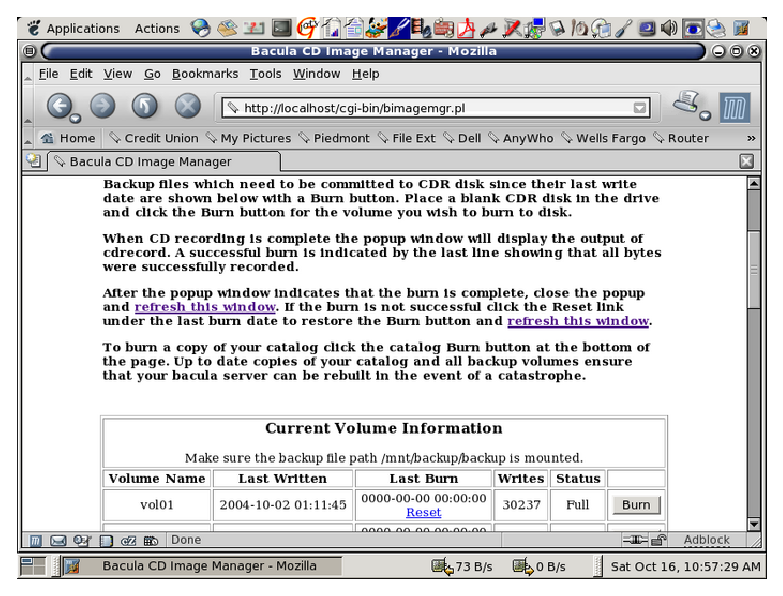
\includegraphics{./bimagemgr1.eps} \\Figure 1 

Place a blank CDR disk in your recorder and click a ``Burn'' button. This will
cause a pop up window as shown in Figure 2 to display the burn progress. 

\addcontentsline{lof}{figure}{Bacula CD Image Burn Progress Window}
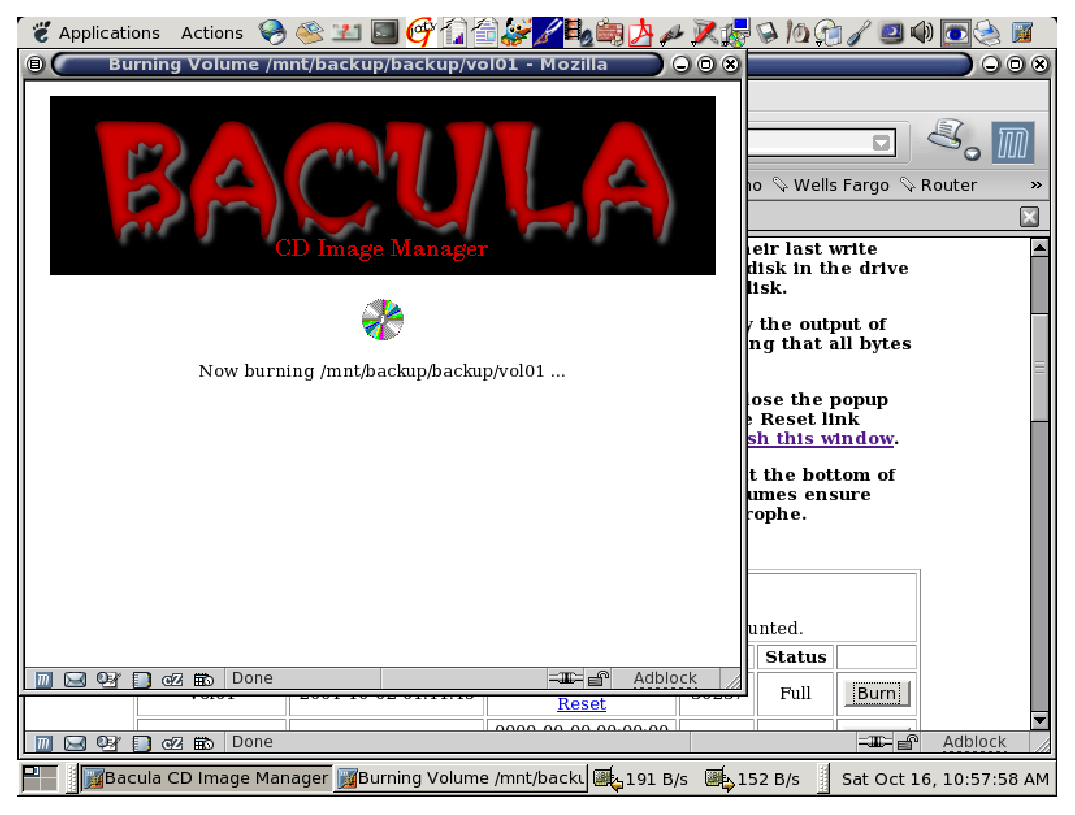
\includegraphics{./bimagemgr2.eps} \\Figure 2 

When the burn finishes the pop up window will display the results of cdrecord
as shown in Figure 3. Close the pop up window and refresh the main window. The
last burn date will be updated and the ``Burn'' button for that volume will
disappear. Should you have a failed burn you can reset the last burn date of
that volume by clicking it's ``Reset'' link. 

\addcontentsline{lof}{figure}{Bacula CD Image Burn Results}
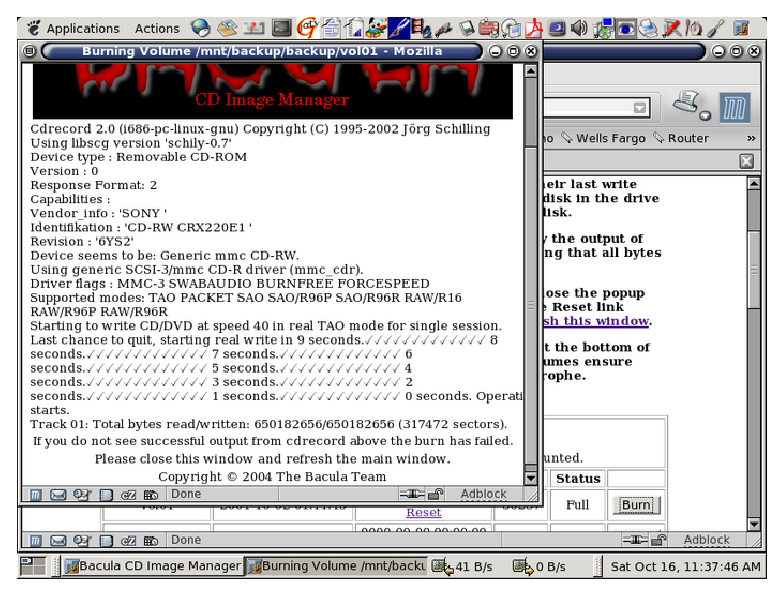
\includegraphics{./bimagemgr3.eps} \\Figure 3 

In the bottom row of the main display window are two more buttons labeled
``Burn Catalog'' and ``Blank CDRW''. ``Burn Catalog'' will place a copy of
your bacula catalog on a disk. If you use CDRW disks rather than CDR then
``Blank CDRW'' allows you to erase the disk before re-burning it. Regularly
committing your backup volume files and your catalog to disk with {\bf
bimagemgr} insures that you can rebuild easily in the event of some disaster
on the bacula server itself. 

%%
%%

\section*{Testing Your Tape Drive With Bacula}
\label{_ChapterStart27}
\index[general]{Testing Your Tape Drive With Bacula }
\addcontentsline{toc}{section}{Testing Your Tape Drive With Bacula}

This chapter is concerned with testing and configuring your tape drive to make
sure that it will work properly with Bacula using the {\bf btape} program. 
\label{summary}

\subsection*{Summary of Steps to Take to Get Your Tape Drive Working}
\index[general]{Working!Summary of Steps to Take to Get Your Tape Drive }
\index[general]{Summary of Steps to Take to Get Your Tape Drive Working }
\addcontentsline{toc}{subsection}{Summary of Steps to Take to Get Your Tape
Drive Working}

In general, you should follow the following steps to get your tape drive to
work with Bacula. Start with a tape mounted in your drive. If you have an
autochanger, load a tape into the drive. We use {\bf /dev/nst0} as the tape
drive name, you will need to adapt it according to your system. 

Do not proceed to the next item until you have succeeded with the previous
one. 

\begin{enumerate}
\item Use tar to write to, then read from your drive:  

   \footnotesize
\begin{verbatim}
   mt -f /dev/nst0 rewind
   tar cvf /dev/nst0 .
   mt -f /dev/nst0 rewind
   tar tvf /dev/nst0
   
\end{verbatim}
\normalsize

\item Make sure you have a valid and correct Device resource  corresponding to
   your drive. For Linux users, generally,  the default one works. For FreeBSD
   users, there are two  possible Device configurations (see below). 
\item Run the btape {\bf test} command:  

   \footnotesize
\begin{verbatim}
   ./btape -c bacula-sd.conf /dev/nst0
   test
   
\end{verbatim}
\normalsize

It isn't necessary to run the autochanger part of the  test at this time,  but
do not go past this point until the basic test succeeds. 
\item Run the btape {\bf fill} command, preferrably with two volumes.  This
   can take a long time. If you have an autochanger and it  is configured, Bacula
   will automatically use it. If you do  not have it configured, you can manual
issue the appopriate  {\bf mtx} command, or press the autochanger buttons to
change  the tape when requested to do so. 
\item FreeBSD users, run the {\bf tapetest} program, and make  sure your
   system is patched if necessary. See below for more  details. 
\item Run Bacula, and backup a reasonably small directory,  say 60 Megabytes.
   Do three successive backups of this  directory. 
\item Stop Bacula, then restart it. Do another full backup  of the same
   directory. Then stop and restart Bacula. 
\item Do a restore of the directory backed up, by entering the  following
   restore command, being careful to restore it to  an alternate location:  

\footnotesize
\begin{verbatim}
   restore select all done
   yes
   
\end{verbatim}
\normalsize

Do a {\bf diff} on the restored directory to ensure it is identical  to the
original directory.  
\item If you have an autochanger, you should now go back to the  btape program
   and run the autochanger test:  

\footnotesize
\begin{verbatim}
     ./btape -c bacula-sd.conf /dev/nst0
     auto
     
\end{verbatim}
\normalsize

Adjust your autochanger as necessary to ensure that it works  correctly. See
the Autochanger chapter of this manual  for a complete discussion of testing
your autochanger.  
\end{enumerate}

If you have reached this point, you stand a good chance of having everything
work. If you get into trouble at any point, {\bf carefully} read the
documentation given below. If you cannot get past some point, ask the {\bf
bacula-users} email list, but specify which of the steps you have successfully
completed. In particular, you may want to look at the 
\ilink{ Tips for Resolving Problems}{problems1} section below. 

\subsubsection*{Specifying the Configuration File}
\index[general]{File!Specifying the Configuration }
\index[general]{Specifying the Configuration File }
\addcontentsline{toc}{subsubsection}{Specifying the Configuration File}

Starting with version 1.27, each of the tape utility programs including the
{\bf btape} program requires a valid Storage daemon configuration file
(actually, the only part of the configuration file that {\bf btape} needs is
the {\bf Device} resource definitions). This permits {\bf btape} to find the
configuration parameters for your archive device (generally a tape drive).
Without those parameters, the testing and utility programs do not no how to
properly read and write your drive. By default, they use {\bf bacula-sd.conf}
in the current directory, but you may specify a different configuration file
using the {\bf -c} option. 

\subsubsection*{Specifying a Device Name For a Tape}
\index[general]{Tape!Specifying a Device Name For a }
\index[general]{Specifying a Device Name For a Tape }
\addcontentsline{toc}{subsubsection}{Specifying a Device Name For a Tape}

{\bf btape} {\bf device-name} where the Volume can be found. In the case of a
tape, this is the physical device name such as {\bf /dev/nst0} or {\bf
/dev/rmt/0ubn} depending on your system that you specify on the Archive Device
directive. For the program to work, it must find the identical name in the
Device resource of the configuration file. If the name is not found in the
list of phsical names, the utility program will compare the name you entered
to the Device names (rather than the Archive device names). See below for
specifying Volume names. 

\subsubsection*{Specifying a Device Name For a File}
\index[general]{File!Specifying a Device Name For a }
\index[general]{Specifying a Device Name For a File }
\addcontentsline{toc}{subsubsection}{Specifying a Device Name For a File}

If you are attempting to read or write an archive file rather than a tape, the
{\bf device-name} should be the full path to the archive location including
the filename. The filename (last part of the specification) will be stripped
and used as the Volume name, and the path (first part before the filename)
must have the same entry in the configuration file. So, the path is equivalent
to the archive device name, and the filename is equivalent to the volume name.


\subsection*{btape}
\label{btape1}
\index[general]{Btape }
\addcontentsline{toc}{subsection}{btape}

This program permits a number of elementary tape operations via a tty command
interface. The {\bf test} command, described below, can be very useful for
testing tape drive compatibility problems. Aside from initial testing of tape
drive compatibility with {\bf Bacula}, {\bf btape} will be mostly used by
developers writing new tape drivers. 

{\bf btape} can be dangerous to use with existing {\bf Bacula} tapes because
it will relabel a tape or write on the tape if so requested regardless of
whether or not the tape contains valuable data, so please be careful and use
it only on blank tapes. 

To work properly, {\bf btape} needs to read the Storage daemon's configuration
file. As a default, it will look for {\bf bacula-sd.conf} in the current
directory. If your configuration file is elsewhere, please use the {\bf -c}
option to specify where. 

The physical device name or the Device resource name must be specified on the
command line, and that this same device name must be present in the Storage
daemon's configuration file read by {\bf btape} 

\footnotesize
\begin{verbatim}
Usage: btape [options] device_name
       -b <file>   specify bootstrap file
       -c <file>   set configuration file to file
       -d <nn>     set debug level to nn
       -s          turn off signals
       -v          be verbose
       -?          print this message.
\end{verbatim}
\normalsize

\subsubsection*{Using btape to Verify your Tape Drive}
\index[general]{Using btape to Verify your Tape Drive }
\index[general]{Drive!Using btape to Verify your Tape }
\addcontentsline{toc}{subsubsection}{Using btape to Verify your Tape Drive}

An important reason for this program is to ensure that a Storage daemon
configuration file is defined so that Bacula will correctly read and write
tapes. 

It is highly recommended that you run the {\bf test} command before running
your first Bacula job to ensure that the parameters you have defined for your
storage device (tape drive) will permit {\bf Bacula} to function properly. You
only need to mount a blank tape, enter the command, and the output should be
reasonably self explanatory. For example: 

\footnotesize
\begin{verbatim}
(ensure that Bacula is not running)
./btape -c /usr/bin/bacula/bacula-sd.conf /dev/nst0
\end{verbatim}
\normalsize

The output will be: 

\footnotesize
\begin{verbatim}
Tape block granularity is 1024 bytes.
btape: btape.c:376 Using device: /dev/nst0
*
\end{verbatim}
\normalsize

Enter the test command: 

\footnotesize
\begin{verbatim}
test
\end{verbatim}
\normalsize

The output produced should be something similar to the following: I've cut the
listing short because it is frequently updated to have new tests. 

\footnotesize
\begin{verbatim}
=== Append files test ===
This test is essential to Bacula.
I'm going to write one record  in file 0,
                   two records in file 1,
             and three records in file 2
btape: btape.c:387 Rewound /dev/nst0
btape: btape.c:855 Wrote one record of 64412 bytes.
btape: btape.c:857 Wrote block to device.
btape: btape.c:410 Wrote EOF to /dev/nst0
btape: btape.c:855 Wrote one record of 64412 bytes.
btape: btape.c:857 Wrote block to device.
btape: btape.c:855 Wrote one record of 64412 bytes.
btape: btape.c:857 Wrote block to device.
btape: btape.c:410 Wrote EOF to /dev/nst0
btape: btape.c:855 Wrote one record of 64412 bytes.
btape: btape.c:857 Wrote block to device.
btape: btape.c:855 Wrote one record of 64412 bytes.
btape: btape.c:857 Wrote block to device.
btape: btape.c:855 Wrote one record of 64412 bytes.
btape: btape.c:857 Wrote block to device.
btape: btape.c:410 Wrote EOF to /dev/nst0
btape: btape.c:387 Rewound /dev/nst0
btape: btape.c:693 Now moving to end of media.
btape: btape.c:427 Moved to end of media
We should be in file 3. I am at file 3. This is correct!
Now the important part, I am going to attempt to append to the tape.
...
=== End Append files test ===
\end{verbatim}
\normalsize

If you do not successfully complete the above test, please resolve the
problem(s) before attempting to use {\bf Bacula}. Depending on your tape
drive, the test may recommend that you add certain records to your
configuration. We strongly recommend that you do so and then re-run the above
test to insure it works the first time. 

Some of the suggestions it provides for resolving the problems may or may not
be useful. If at all possible avoid using fixed blocking. If the test suddenly
starts to print a long series of: 

\footnotesize
\begin{verbatim}
Got EOF on tape.
Got EOF on tape.
...
\end{verbatim}
\normalsize

then almost certainly, you are running your drive in fixed block mode rather
than variable block mode. Please see below for help on resolving that. 

For FreeBSD users, please see the notes below for doing further testing of
your tape drive. 

\subsubsection*{Linux SCSI Tricks}
\index[general]{Tricks!Linux SCSI }
\index[general]{Linux SCSI Tricks }
\addcontentsline{toc}{subsubsection}{Linux SCSI Tricks}

You can find out what SCSI devices you have by doing: 

\footnotesize
\begin{verbatim}
cat /proc/scsi/scsi
\end{verbatim}
\normalsize

For example, I get the following: 

\footnotesize
\begin{verbatim}
Attached devices:
Host: scsi2 Channel: 00 Id: 01 Lun: 00
  Vendor: HP       Model: C5713A           Rev: H107
  Type:   Sequential-Access                ANSI SCSI revision: 02
Host: scsi2 Channel: 00 Id: 04 Lun: 00
  Vendor: SONY     Model: SDT-10000        Rev: 0110
  Type:   Sequential-Access                ANSI SCSI revision: 02
\end{verbatim}
\normalsize

If you want to remove the SDT-10000 device, you can do so as root with: 

\footnotesize
\begin{verbatim}
echo "scsi remove-single-device 2 0 4 0">/proc/scsi/scsi
\end{verbatim}
\normalsize

and you can put add it back with: 

\footnotesize
\begin{verbatim}
echo "scsi add-single-device 2 0 4 0">/proc/scsi/scsi
\end{verbatim}
\normalsize

where the 2 0 4 0 are the Host, Channel, Id, and Lun as seen on the output
from {\bf cat /proc/scsi/scsi}. Note, the Channel must be specified as
numeric. 
\label{problems1}

\subsection*{Tips for Resolving Problems}
\index[general]{Problems!Tips for Resolving }
\index[general]{Tips for Resolving Problems }
\addcontentsline{toc}{subsection}{Tips for Resolving Problems}

\label{CannotRestore}

\subsubsection*{Bacula Saves But Cannot Restore Files}
\index[general]{Files!Bacula Saves But Cannot Restore }
\index[general]{Bacula Saves But Cannot Restore Files }
\addcontentsline{toc}{subsubsection}{Bacula Saves But Cannot Restore Files}

If you are getting error messages such as: 

\footnotesize
\begin{verbatim}
Volume data error at 0:1! Wanted block-id: "BB02", got "". Buffer discarded
\end{verbatim}
\normalsize

It is very likely that Bacula has tried to do block positioning and ended up
at an invalid block. This can happen if your tape drive is in fixed block mode
while Bacula's default is variable blocks. Note that in such cases, Bacula is
perfectly able to write to your Volumes (tapes), but cannot position to read
them. 

There are two possible solutions. 

\begin{enumerate}
\item The first and  best is to always ensure that your drive is in  variable
   block mode. Note, it can switch back to  fixed block mode on a reboot or if
   another program  uses the drive. So on such systems you  need to modify the
Bacula startup files  to explicitly set: 

\footnotesize
\begin{verbatim}
mt -f /dev/nst0 defblksize 0
\end{verbatim}
\normalsize

or whatever is appropriate on your system.  
\item The second possibility, especially, if Bacula wrote  while the drive was
   in fixed block mode, is to turn  off block positioning in Bacula. This is done
   by  adding: 

\footnotesize
\begin{verbatim}
Block Positioning = no
\end{verbatim}
\normalsize

to the Device resource. This is not the recommended  procedure because it can
enormously slow down  recovery of files, but it may help where all else 
fails. This directive is available in version 1.35.5  or later (and not yet
tested).  
\end{enumerate}

\label{opendevice}

\subsubsection*{Bacula Cannot Open the Device}
\index[general]{Device!Bacula Cannot Open the }
\index[general]{Bacula Cannot Open the Device }
\addcontentsline{toc}{subsubsection}{Bacula Cannot Open the Device}

If you get an error message such as: 

\footnotesize
\begin{verbatim}
dev open failed: dev.c:265 stored: unable to open
device /dev/nst0:> ERR=No such device or address
\end{verbatim}
\normalsize

the first time you run a job, it is most likely due to the fact that you
specified the incorrect device name on your {\bf Archive Device}. 

If Bacula works fine with your drive, then all off a sudden you get error
messages similar to the one shown above, it is quite possible that your driver
module is being removed because the kernel deems it idle. This is done via
{\bf crontab} with the use of {\bf rmmod -a}. To fix the problem, you can
remove this entry from {\bf crontab}, or you can manually {\bf modprob} your
driver module (or add it to the local startup script). Thanks to Alan Brown
for this tip. 
\label{IncorrectFiles}

\subsubsection*{Incorrect File Number}
\index[general]{Number!Incorrect File }
\index[general]{Incorrect File Number }
\addcontentsline{toc}{subsubsection}{Incorrect File Number}

When Bacula moves to the end of the medium, it normally uses the {\bf
ioctl(MTEOM)} function. Then Bacula uses the {\bf ioctl(MTIOCGET)} function to
retrieve the current file position from the {\bf mt\_fileno} field. Some SCSI
tape drivers will use a fast means of seeking to the end of the medium and in
doing so, they will not know the current file position and hence return a {\bf
-1}. As a consequence, if you get {\bf ``This is NOT correct!''} in the
positioning tests, this may be the cause. You must correct this condition in
order for Bacula to work. 

There are two possible solutions to the above problem of incorrect file
number: 

\begin{itemize}
\item Figure out how to configure your SCSI driver to  keep track of the file
   position during the MTEOM  request. This is the preferred solution.  
\item Modify the {\bf Device} resource of your {\bf bacula-sd.conf} file  to
   include:  

\footnotesize
\begin{verbatim}
Hardware End of File = no
\end{verbatim}
\normalsize

This will cause Bacula to use the MTFSF request to  seek to the end of the
medium, and Bacula will keep  track of the file number itself. 
\end{itemize}

\label{IncorrectBlocks}

\subsubsection*{Incorrect Number of Blocks or Positioning Errors during btape
Testing}
\index[general]{Testing!Incorrect Number of Blocks or Positioning Errors
during btape }
\index[general]{Incorrect Number of Blocks or Positioning Errors during btape
Testing }
\addcontentsline{toc}{subsubsection}{Incorrect Number of Blocks or Positioning
Errors during btape Testing}

{\bf Bacula's} preferred method of working with tape drives (sequential
devices) is to run in variable block mode, and this is what is set by default.
You should first ensure that your tape drive is set for variable block mode
(see below). 

If your tape drive is in fixed block mode and you have told Bacula to use
different fixed block sizes or variable block sizes (default), you will get
errors when Bacula attempts to forward space to the correct block (the kernel
driver's idea of tape blocks will not correspond to Bacula's). 

All modern tape drives support variable tape blocks, but some older drives (in
particular the QIC drives) as well as the ATAPI ide-scsi driver run only in
fixed block mode. The Travan tape drives also apparently must run in fixed
block mode (to be confirmed). 

Even in variable block mode, with the exception of the first record on the
second or subsequent volume of a multi-volume backup, Bacula will write blocks
of a fixed size. However, in reading a tape, Bacula will assume that for each
read request, exactly one block from the tape will be transferred. This the
most common way that tape drives work and is well supported by {\bf Bacula}. 

Drives that run in fixed block mode can cause serious problems for Bacula if
the drive's block size does not correspond exactly to {\bf Bacula's} block
size. In fixed block size mode, drivers may transmit a partial block or
multiple blocks for a single read request. From {\bf Bacula's} point of view,
this destroys the concept of tape blocks. It is much better to run in variable
block mode, and almost all modern drives (the OnStream is an exception) run in
variable block mode. In order for Bacula to run in fixed block mode, you must
include the following records in the Storage daemon's Device resource
definition: 

\footnotesize
\begin{verbatim}
Minimum Block Size = nnn
Maximum Block Size = nnn
\end{verbatim}
\normalsize

where {\bf nnn} must be the same for both records and must be identical to the
driver's fixed block size. 

We recommend that you avoid this configuration if at all possible by using
variable block sizes. 

If you must run with fixed size blocks, make sure they are not 512 bytes. This
is too small and the overhead that Bacula has with each record will become
excessive. If at all possible set any fixed block size to something like
64,512 bytes or possibly 32,768 if 64,512 is too large for your drive. See
below for the details on checking and setting the default drive block size. 

To recover files from tapes written in fixed block mode, see below. 
\label{TapeModes}

\subsubsection*{Ensuring that the Tape Modes Are Properly Set -- {\bf Linux
Only}}
\index[general]{Ensuring that the Tape Modes Are Properly Set -- Linux Only }
\index[general]{Only!Ensuring that the Tape Modes Are Properly Set -- Linux }
\addcontentsline{toc}{subsubsection}{Ensuring that the Tape Modes Are Properly
Set -- Linux Only}

If you have a modern SCSI tape drive and you are having problems with the {\bf
test} command as noted above, it may be that some program has set one or more
of the your SCSI driver's options to non-default values. For example, if your
driver is set to work in SysV manner, Bacula will not work correctly because
it expects BSD behavior. To reset your tape drive to the default values, you
can try the following, but {\bf ONLY} if you have a SCSI tape drive on a {\bf
Linux} system: 

\footnotesize
\begin{verbatim}
become super user
mt -f /dev/nst0 rewind
mt -f /dev/nst0 stoptions buffer-writes async-writes read-ahead
\end{verbatim}
\normalsize

The above commands will clear all options and then set those specified. None
of the specified options are required by Bacula, but a number of other options
such as SysV behavior must not be set. Bacula does not support SysV tape
behavior. On systems other than Linux, you will need to consult your {\bf mt}
man pages or documentation to figure out how to do the same thing. This should
not really be necessary though -- for example, on both Linux and Solaris
systems, the default tape driver options are compatible with Bacula. 

You may also want to ensure that no prior program has set the default block
size, as happened to one user, by explicitly turning it off with: 

\footnotesize
\begin{verbatim}
mt -f /dev/nst0 defblksize 0
\end{verbatim}
\normalsize

If you would like to know what stoptions you have set before making any of the
changes noted above, you can now view them on Linux systems, thanks to a tip
provided by Willem Riede. Do the following: 

\footnotesize
\begin{verbatim}
become super user
mt -f /dev/nst0 stsetoptions 0
grep st0 /var/log/messages
\end{verbatim}
\normalsize

and you will get output that looks something like the following: 

\footnotesize
\begin{verbatim}
kernel: st0: Mode 0 options: buffer writes: 1, async writes: 1, read ahead: 1
kernel: st0:    can bsr: 0, two FMs: 0, fast mteom: 0, auto lock: 0,
kernel: st0:    defs for wr: 0, no block limits: 0, partitions: 0, s2 log: 0
kernel: st0:    sysv: 0 nowait: 0
\end{verbatim}
\normalsize

Note, I have chopped off the beginning of the line with the date and machine
name for presentation purposes. 

Some people find that the above settings only last until the next reboot, so
please check this otherwise you may have unexpected problems. 

Beginning with Bacula version 1.35.8, if Bacula detects that you are running
in variable block mode, it will attempt to set your drive appropriately. All
OSes permit setting variable block mode, but some OSes do not permit setting
the other modes that Bacula needs to function properly. 
\label{compression}

\subsubsection*{Checking and Setting Tape Hardware Compression and Blocking
Size}
\index[general]{Checking and Setting Tape Hardware Compression and Blocking
Size }
\index[general]{Size!Checking and Setting Tape Hardware Compression and
Blocking }
\addcontentsline{toc}{subsubsection}{Checking and Setting Tape Hardware
Compression and Blocking Size}

As far as I can tell, there is no way with the {\bf mt} program to check if
your tape hardware compression is turned on or off. You can, however, turn it
on by using (on Linux): 

\footnotesize
\begin{verbatim}
become super user
mt -f /dev/nst0 defcompression 1
\end{verbatim}
\normalsize

and of course, if you use a zero instead of the one at the end, you will turn
it off. 

You may also want to ensure that no prior program has set the default block
size, as happened to one user, by explicitly turning it off with: 

\footnotesize
\begin{verbatim}
mt -f /dev/nst0 defblksize 0
\end{verbatim}
\normalsize

If you have built the {\bf mtx} program in the {\bf depkgs} package, you can
use tapeinfo to get quite a bit of information about your tape drive even if
it is not an autochanger. This program is called using the SCSI control
device. On Linux for tape drive /dev/nst0, this is usually /dev/sg0, while on
FreeBSD for /dev/nsa0, the control device is often /dev/pass2. For example on
my DDS-4 drive (/dev/nst0), I get the following: 

\footnotesize
\begin{verbatim}
tapeinfo -f /dev/sg0
Product Type: Tape Drive
Vendor ID: 'HP      '
Product ID: 'C5713A          '
Revision: 'H107'
Attached Changer: No
MinBlock:1
MaxBlock:16777215
SCSI ID: 5
SCSI LUN: 0
Ready: yes
BufferedMode: yes
Medium Type: Not Loaded
Density Code: 0x26
BlockSize: 0             
\end{verbatim}
\normalsize

where the {\bf DataCompEnabled: yes} means that tape hardware compression is
turned on. You can see it turn on and off (yes|no) by using the {\bf mt}
commands given above. Also, this output will tell you if the {\bf BlockSize}
is non-zero and hence set for a particular block size. Bacula is not likely to
work in such a situation because it will normally attempt to write blocks of
64,512 bytes, except the last block of the job which will generally be
shorter. The first thing to try is setting the default block size to zero
using the {\bf mt \ -f \ /dev/nst0 \ defblksize \ 0} command as shown above.
On FreeBSD, this would be something like: {\bf mt \ -f \ /dev/nsa0 \ blocksize
\ 0}. 

If your tape drive requires fixed block sizes (very unusual), you can use the
following records: 

\footnotesize
\begin{verbatim}
Minimum Block Size = nnn
Maximum Block Size = nnn
\end{verbatim}
\normalsize

in your Storage daemon's Device resource to force Bacula to write fixed size
blocks (where you sent nnn to be the same for both of the above records). This
should be done only if your drive does not support variable block sizes, or
you have some other strong reasons for using fixed block sizes. As mentioned
above, a small fixed block size of 512 or 1024 bytes will be very inefficient.
Try to set any fixed block size to something like 64,512 bytes or larger if
your drive will support it. 

Also, note that the {\bf Medium Type} field of the output of {\bf tapeinfo}
reports {\bf Not Loaded}, which is not correct. As a consequence, you should
ignore that field as well as the {\bf Attached Changer} field. 

To recover files from tapes written in fixed block mode, see below. 
\label{FreeBSDTapes}

\subsubsection*{Tape Modes on FreeBSD}
\index[general]{FreeBSD!Tape Modes on }
\index[general]{Tape Modes on FreeBSD }
\addcontentsline{toc}{subsubsection}{Tape Modes on FreeBSD}

On most FreeBSD systems such as 4.9 and most tape drives, Bacula should run
with: 

\footnotesize
\begin{verbatim}
mt \  -f \  /dev/nsa0 \  seteotmodel \  2
mt \  -f \  /dev/nsa0 \  blocksize \  0
mt \  -f \ /dev/nsa0 \  comp \  enable
\end{verbatim}
\normalsize

You might want to put those commands in a startup script to make sure your
tape driver is properly initialized before running Bacula. 

Then according to what the {\bf btape test} command returns, you will probably
need to set the following (see below for an alternative): 

\footnotesize
\begin{verbatim}
  Hardware End of Medium = no
  BSF at EOM = yes
  Backward Space Record = no
  Backward Space File = no
  Fast Forward Space File = no
  TWO EOF = yes
\end{verbatim}
\normalsize

Then be sure to run some append tests with Bacula where you start and stop
Bacula between appending to the tape, or use {\bf btape} version 1.35.1 or
greater, which includes simulation of stopping/restarting Bacula. 

Please see the file {\bf platforms/freebsd/pthreads-fix.txt} in the main
Bacula directory concerning {\bf important} information concerning
compatibility of Bacula and your system. A much more optimal Device
configuration is shown below, but does not work with all tape drives. Please
test carefully before putting either into production. 

Note, for FreeBSD 4.10-RELEASE, using a Sony TSL11000 L100 DDS4 w/Autochanger
set to variable block size and DCLZ compression, Brian McDonald reports that
to get Bacula to append correctly between Bacula executions, the correct
values to use are: 

\footnotesize
\begin{verbatim}
mt \  -f \  /dev/nsa0 \  seteotmodel \  1
mt \  -f \  /dev/nsa0 \  blocksize \  0
mt \  -f \ /dev/nsa0 \  comp \  enable
\end{verbatim}
\normalsize

and 

\footnotesize
\begin{verbatim}
  Hardware End of Medium = no
  BSF at EOM = no
  Backward Space Record = no
  Backward Space File = no
  Fast Forward Space File = yes
  TWO EOF = no
\end{verbatim}
\normalsize

This has been confirmed by several other people using different hardware. This
configuration is the preferred one because it uses one EOF and no backspacing
at the end of the tape, which works much more efficiently and reliably with
modern tape drives. 

\subsubsection*{Determining What Tape Drives and Autochangers You Have on
FreeBSD}
\index[general]{FreeBSD!Determining What Tape Drives and Autochangers You Have
on }
\index[general]{Determining What Tape Drives and Autochangers You Have on
FreeBSD }
\addcontentsline{toc}{subsubsection}{Determining What Tape Drives and
Autochangers You Have on FreeBSD}

On FreeBSD, you can do a {\bf camcontrol devlist} as root to determine what
drives and autochangers you have. For example, 

\footnotesize
\begin{verbatim}
undef# camcontrol devlist
    at scbus0 target 2 lun 0 (pass0,sa0)
    at scbus0 target 4 lun 0 (pass1,sa1)
    at scbus0 target 4 lun 1 (pass2)
\end{verbatim}
\normalsize

from the above, you can determine that there is a tape drive on {\bf /dev/sa0}
and another on {\bf /dev/sa1} in addition since there is a second line for the
drive on {\bf /dev/sa1}, you know can assume that it is the control device for
the autochanger (i.e. {\bf /dev/pass2}). It is also the control device name to
use when invoking the tapeinfo program. E.g. 

\footnotesize
\begin{verbatim}
tapeinfo -f /dev/pass2
\end{verbatim}
\normalsize

\label{onstream}

\subsubsection*{Using the OnStream driver on Linux Systems}
\index[general]{Using the OnStream driver on Linux Systems }
\index[general]{Systems!Using the OnStream driver on Linux }
\addcontentsline{toc}{subsubsection}{Using the OnStream driver on Linux
Systems}

Bacula version 1.33 (not 1.32x) is now working and ready for testing with the
OnStream kernel osst driver version 0.9.14 or above. Osst is available from: 
\elink{http://sourceforge.net/projects/osst/}{http://sourceforge.net/projects/%
osst/}. 

To make Bacula work you must first load the new driver then, as root, do: 

\footnotesize
\begin{verbatim}
  mt -f /dev/nosst0 defblksize 32768
\end{verbatim}
\normalsize

Also you must add the following to your Device resource in your Storage
daemon's conf file: 

\footnotesize
\begin{verbatim}
 Minimum Block Size = 32768
 Maximum Block Size = 32768
\end{verbatim}
\normalsize

Here is a Device specification provided by Michel Meyers that is known to
work: 

\footnotesize
\begin{verbatim}
Device {
  Name = "Onstream DI-30"
  Media Type = "ADR-30"
  Archive Device = /dev/nosst0
  Minimum Block Size = 32768
  Maximum Block Size = 32768
  Hardware End of Medium = yes
  BSF at EOM = no
  Backward Space File = yes
  Fast Forward Space File = yes
  Two EOF = no
  AutomaticMount = yes
  AlwaysOpen = yes
  Removable Media = yes
}
\end{verbatim}
\normalsize

\label{fill}

\subsubsection*{Using btape to Simulate Bacula Filling a Tape}
\index[general]{Using btape to Simulate Bacula Filling a Tape }
\index[general]{Tape!Using btape to Simulate Bacula Filling a }
\addcontentsline{toc}{subsubsection}{Using btape to Simulate Bacula Filling a
Tape}

Because there are often problems with certain tape drives or systems when end
of tape conditions occur, {\bf btape} has a special command {\bf fill} that
causes it to write random data to a tape until the tape fills. It then writes
at least one more Bacula block to a second tape. Finally, it reads back both
tapes to ensure that the data has been written in a way that Bacula can
recover it. Note, there is also a single tape option as noted below, which you
should use rather than the two tape test. See below for more details. 

This can be an extremely time consuming process (here is is about 6 hours) to
fill a full tape. Note, that btape writes random data to the tape when it is
filling it. This has two consequences: 1. it takes a bit longer to generate
the data, especially on slow CPUs. 2. the total amount of data is
approximately the real physical capacity of your tape, regardless of whether
or not the tape drive compression is on or off. This is because random data
does not compress very much. 

To begin this test, you enter the {\bf fill} command and follow the
instructions. There are two options: the simple single tape option and the
multiple tape option. Please use only the simple single tape option because
the multiple tape option still doesn't work totally correctly. If the single
tape option does not succeed, you should correct the problem before using
Bacula. 
\label{RecoveringFiles}

\subsection*{Recovering Files Written to Tape With Fixed Block Sizes}
\index[general]{Recovering Files Written to Tape With Fixed Block Sizes }
\index[general]{Sizes!Recovering Files Written to Tape With Fixed Block }
\addcontentsline{toc}{subsection}{Recovering Files Written to Tape With Fixed
Block Sizes}

If you have been previously running your tape drive in fixed block mode
(default 512) and Bacula with variable blocks (default), then in version
1.32f-x and 1.34 and above, Bacula will fail to recover files because it does
block spacing, and because the block sizes don't agree between your tape drive
and Bacula it will not work. 

The long term solution is to run your drive in variable block mode as
described above. However, if you have written tapes using fixed block sizes,
this can be a bit of a pain. The solution to the problem is: while you are
doing a restore command using a tape written in fixed block size, ensure that
your drive is set to the fixed block size used while the tape was written.
Then when doing the {\bf restore} command in the Console program, do not
answer the prompt {\bf yes/mod/no}. Instead, edit the bootstrap file (the
location is listed in the prompt) using any ASCII editor. Remove all {\bf
VolBlock} lines in the file. When the file is re-written, answer the question,
and Bacula will run without using block positioning, and it should recover
your files. 
\label{BlockModes}

\subsection*{Tape Blocking Modes}
\index[general]{Modes!Tape Blocking }
\index[general]{Tape Blocking Modes }
\addcontentsline{toc}{subsection}{Tape Blocking Modes}

SCSI tapes may either be written in {\bf variable} or {\bf fixed} block sizes.
Newer drives support both modes, but some drives such as the QIC devices
always use fixed block sizes. Bacula attempts to fill and write complete
blocks (default 65K), so that in normal mode (variable block size), Bacula
will always write blocks of the same size except the last block of a Job. If
Bacula is configured to write fixed block sizes, it will pad the last block of
the Job to the correct size. Bacula expects variable tape block size drives to
behave as follows: Each write to the drive results in a single record being
written to the tape. Each read returns a single record. If you request less
byte than are in the record, only those number of bytes will be returned, but
the entire logical record will have been read (the next read will retrieve the
next record). Thus data from a single write is always returned in a single
read, and sequentially written records are returned by sequential reads. 

Bacula expects fixed block size tape drives to behave as follows: If a write
length is greater than the physical block size of the drive, the write will be
written as two blocks each of the fixed physical size. This a single write may
become multiple physical records on the tape. (This is not a good situation).
According to the documentation, one may never write an amount of data that is
not the exact multiple of the blocksize (it is not specified if an error
occurs or if the the last record is padded). When reading, it is my
understanding that each read request reads one physical record from the tape.
Due to the complications of fixed block size tape drives, you should avoid
them if possible with Bacula, or you must be ABSOLUTELY certain that you use
fixed block sizes within Bacula that correspond to the physical block size of
the tape drive. This will ensure that Bacula has a one to one correspondence
between what it writes and the physical record on the tape. 

Please note that Bacula will not function correctly if it writes a block and
that block is split into two or more physical records on the tape. Bacula
assumes that each write causes a single record to be written, and that it can
sequentially recover each of the blocks it has written by using the same
number of sequential reads as it had written. 

%%
%%

\section*{What To Do When Bacula Crashes (Kaboom)}
\label{_ChapterStart47}
\index[general]{Kaboom!What To Do When Bacula Crashes }
\index[general]{What To Do When Bacula Crashes (Kaboom) }
\addcontentsline{toc}{section}{What To Do When Bacula Crashes (Kaboom)}

If you are running on a Linux system, and you have a set of working
configuration files, it is very unlikely that {\bf Bacula} will crash. As with
all software, however, it is inevitable that someday, it may crash,
particularly if you are running on another operating system or using a new or
unusual feature. 

This chapter explains what you should do if one of the three {\bf Bacula}
daemons (Director, File, Storage) crashes. 

\subsection*{Traceback}
\index[general]{Traceback }
\addcontentsline{toc}{subsection}{Traceback}

Each of the three Bacula daemons has a built-in exception handler which, in
case of an error, will attempt to produce a traceback. If successful the
traceback will be emailed to you. 

For this to work, you need to ensure that a few things are setup correctly on
your system: 

\begin{enumerate}
\item You must have an installed copy of {\bf gdb} (the GNU debugger),  and it
   must be on {\bf Bacula's} path. 
\item The Bacula installed script file {\bf btraceback} must  be in the same
   directory as the daemon which dies, and it must  be marked as executable.  
\item The script file {\bf btraceback.gdb} must  have the correct  path to it
   specified in the {\bf btraceback} file.  
\item You must have a {\bf mail} program which is on {\bf Bacula's}  path. 
   \end{enumerate}

If all the above conditions are met, the daemon that crashes will produce a
traceback report and email it to you. If the above conditions are not true,
you can either run the debugger by hand as described below, or you may be able
to correct the problems by editing the {\bf btraceback} file. I recommend not
spending too much time on trying to get the traceback to work as it can be
very difficult. 

The changes that might needed are to add a correct path to the {\bf gdb}
program, correct the path to the {\bf btraceback.gdb} file, change the {\bf
mail} program or its path, or change your email address. The key line in the
{\bf btraceback} file is: 

\footnotesize
\begin{verbatim}
gdb -quiet -batch -x /home/kern/bacula/bin/btraceback.gdb \
     $1 $2 2>\&1 | mail -s "Bacula traceback" your-address@xxx.com
\end{verbatim}
\normalsize

Since each daemon has the same traceback code, a single btraceback file is
sufficient if you are running more than one daemon on a machine. 

\subsection*{Testing The Traceback}
\index[general]{Traceback!Testing The }
\index[general]{Testing The Traceback }
\addcontentsline{toc}{subsection}{Testing The Traceback}

To ``manually'' test the traceback feature, you simply start {\bf Bacula} then
obtain the {\bf PID} of the main daemon thread (there are multiple threads).
Unfortunately, the output had to be split to fit on this page: 

\footnotesize
\begin{verbatim}
[kern@rufus kern]$ ps fax --columns 132 | grep bacula-dir
 2103 ?        S      0:00 /home/kern/bacula/k/src/dird/bacula-dir -c
                                       /home/kern/bacula/k/src/dird/dird.conf
 2104 ?        S      0:00  \_ /home/kern/bacula/k/src/dird/bacula-dir -c
                                       /home/kern/bacula/k/src/dird/dird.conf
 2106 ?        S      0:00      \_ /home/kern/bacula/k/src/dird/bacula-dir -c
                                       /home/kern/bacula/k/src/dird/dird.conf
 2105 ?        S      0:00      \_ /home/kern/bacula/k/src/dird/bacula-dir -c
                                       /home/kern/bacula/k/src/dird/dird.conf
\end{verbatim}
\normalsize

which in this case is 2103. Then while Bacula is running, you call the program
giving it the path to the Bacula executable and the {\bf PID}. In this case,
it is: 

\footnotesize
\begin{verbatim}
./btraceback /home/kern/bacula/k/src/dird 2103
\end{verbatim}
\normalsize

It should produce an email showing you the current state of the daemon (in
this case the Director), and then exit leaving {\bf Bacula} running as if
nothing happened. If this is not the case, you will need to correct the
problem by modifying the {\bf btraceback} script. 

Typical problems might be that {\bf gdb} is not on the default path. Fix this
by specifying the full path to it in the {\bf btraceback} file. Another common
problem is that the {\bf mail} program doesn't work or is not on the default
path. On some systems, it is preferable to use {\bf Mail} rather than {\bf
mail}. 

\subsection*{Getting A Traceback On Other Systems}
\index[general]{Getting A Traceback On Other Systems }
\index[general]{Systems!Getting A Traceback On Other }
\addcontentsline{toc}{subsection}{Getting A Traceback On Other Systems}

It should be possible to produce a similar traceback on systems other than
Linux, either using {\bf gdb} or some other debugger. Solaris with {\bf gdb}
loaded works quite fine. On other systems, you will need to modify the {\bf
btraceback} program to invoke the correct debugger, and possibly correct the
{\bf btraceback.gdb} script to have appropriate commands for your debugger. If
anyone succeeds in making this work with another debugger, please send us a
copy of what you modified. 
\label{ManuallyDebugging}

\subsection*{Manually Running Bacula Under The Debugger}
\index[general]{Manually Running Bacula Under The Debugger }
\index[general]{Debugger!Manually Running Bacula Under The }
\addcontentsline{toc}{subsection}{Manually Running Bacula Under The Debugger}

If for some reason you cannot get the automatic traceback, or if you want to
interactively examine the variable contents after a crash, you can run Bacula
under the debugger. Assuming you want to run the Storage daemon under the
debugger (the technique is the same for the other daemons, only the name
changes), you would do the following: 

\begin{enumerate}
\item Start the Director and the File daemon. If the  Storage daemon also
   starts, you will need to find its PID  as shown above (ps fax | grep
   bacula-sd) and kill it  with a command like the following:  

\footnotesize
\begin{verbatim}
      kill -15 PID
      
\end{verbatim}
\normalsize

where you replace {\bf PID} by the actual value. 
\item At this point, the Director and the File daemon should  be running but
   the Storage daemon should not.  
\item cd to the directory containing the Storage daemon  
\item Start the Storage daemon under the debugger:  

   \footnotesize
\begin{verbatim}
    gdb ./bacula-sd
    
\end{verbatim}
\normalsize

\item Run the Storage daemon:  

   \footnotesize
\begin{verbatim}
     run -s -f -c ./bacula-sd.conf
     
\end{verbatim}
\normalsize

You may replace the {\bf ./bacula-sd.conf} with the full path  to the Storage
daemon's configuration file.  
\item At this point, Bacula will be fully operational.  
\item In another shell command window, start the Console program  and do what
   is necessary to cause Bacula to die.  
\item When Bacula crashes, the {\bf gdb} shell window will  become active and
   {\bf gdb} will show you the error that  occurred.  
\item To get a general traceback of all threads, issue the following  command:
 

\footnotesize
\begin{verbatim}
       thread apply all bt
       
\end{verbatim}
\normalsize

After that you can issue any debugging command. 
\end{enumerate}

\subsection*{Getting Debug Output from Bacula}
\index[general]{Getting Debug Output from Bacula }
\addcontentsline{toc}{subsection}{Getting Debug Output from Bacula}

Each of the daemons normally has debug compiled into the program, but
disabled. There are two ways to enable the debug output. One is to add the
{\bf -d nnn} option on the command line when starting the debugger. The {\bf
nnn} is the debug level, and generally anything between 50 and 200 is
reasonable. The higher the number, the more output is produced. The output is
written to standard output. 

The second way of getting debug output is to dynamically turn it on using the
Console using the {\bf setdebug} command. The full syntax of the command is: 

\footnotesize
\begin{verbatim}
 setdebug level=nnn client=client-name storage=storage-name dir
\end{verbatim}
\normalsize

If none of the options are given, the command will prompt you. You can
selectively turn on/off debugging in any or all the daemons (i.e. it is not
necessary to specify all the components of the above command). 

%%
%%

\section*{The Windows Version of Bacula}
\label{_ChapterStart7}
\index[general]{Windows Version of Bacula }
\addcontentsline{toc}{section}{Windows Version of Bacula}

\subsection*{General}
\index[general]{General }
\addcontentsline{toc}{subsection}{General}

At the current time only the File daemon or Client program has been tested on
Windows. As a consequence, when we speak of the Windows version of Bacula
below, we are referring to the File daemon only. 

The Windows version of the Bacula File daemon has been tested on Win98, WinMe,
WinNT, and Win2000 systems. We have coded to support Win95, but no longer have
a system for testing. The Windows version of Bacula is a native Win32 port,
but there are very few source code changes, which means that the Windows
version is for the most part running code that has long proved stable on Unix
systems. When running, it is perfectly integrated with Windows and displays
its icon in the system icon tray, and provides a system tray menu to obtain
additional information on how Bacula is running (status and events dialog
boxes). If so desired, it can also be stopped by using the system tray menu,
though this should normally never be necessary. 

Once installed Bacula normally runs as a system service. This means that it is
immediately started by the operating system when the system is booted, and
runs in the background even if there is no user logged into the system. 

\subsubsection*{Win32 Installation}
\label{installation}
\index[general]{Installation }
\index[general]{Win32!Installation }
\addcontentsline{toc}{subsubsection}{Win32 Installation}

Normally, you will install the Windows version of Bacula from the binaries.
This install is standard Windows .exe that runs an install wizard using the
NSIS Free Software installer, so if you have already installed Windows
software, it should be very familiar to you. 

If you have a previous version Cygwin of Bacula (1.32 or lower) installed, you
should stop the service, uninstall it, and remove the directory possibly
saving your bacula-fd.conf file for use with the new version you will install.
The new native version of Bacula has far fewer files than the old Cygwin
version. 

Finally, proceed with the installation. 

\begin{itemize}
\item Simply double click on the {\bf winbacula-1.xx.0.exe}  NSIS install
   icon. The  actual name of the icon will vary from one release version to 
   another. 


\includegraphics{./win32-nsis.eps}  winbacula-1.xx.0.exe  
\ 
\item Once launched, the installer wizard will ask you if you want  to install
   Bacula.  

\addcontentsline{lof}{figure}{Win32 Client Setup Wizard}
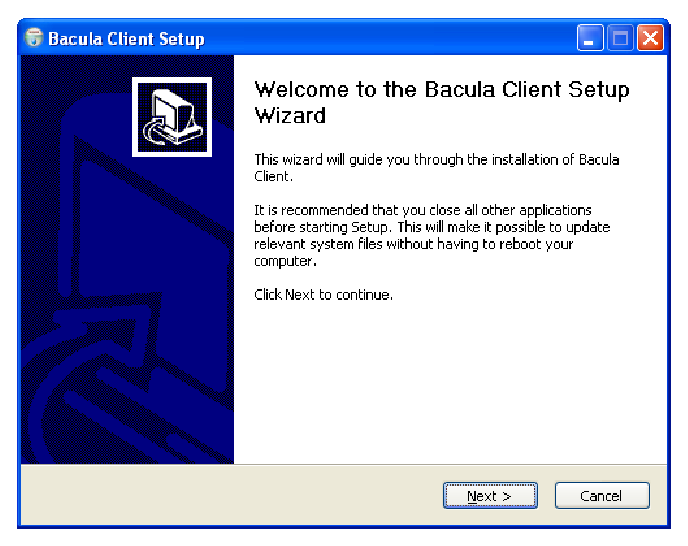
\includegraphics{./win32-welcome.eps}  
\ 
\item If you proceed, you will be asked to select the components to be 
   installed. You may install the Bacula program (Bacula File Service)  and or
   the documentation. Both will be installed in sub-directories  of the install
location that you choose later. The components  dialog looks like the
following:  

\addcontentsline{lof}{figure}{Win32 Component Selection Dialog}
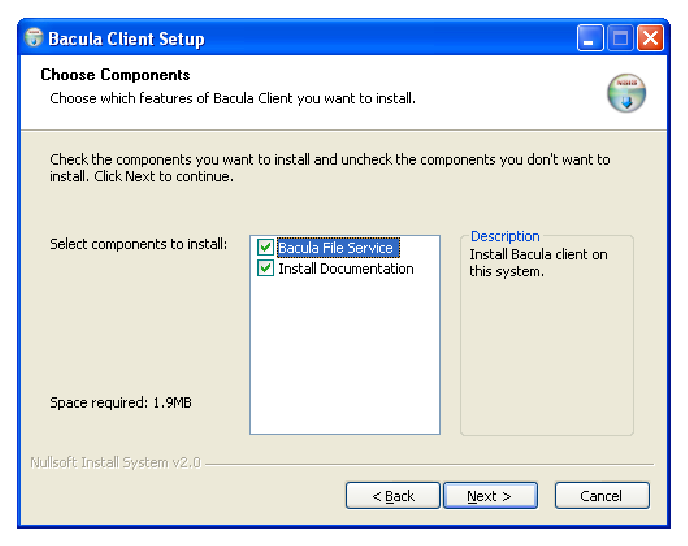
\includegraphics{./win32-pkg.eps}  

\item Next you will be asked to select an installation directory.  

   \addcontentsline{lof}{figure}{Win32 Directory Selection Dialog}

\includegraphics{./win32-location.eps}  

\item If you are installing for the first time, you will  be asked if you want
   to edit the bacula-fd.conf file, and  if you respond with yes, it will be
   opened in notepad.  
\ 
\item Then the installer will ask if wish to install Bacula as a  service. You
   should always choose to do so:  

\addcontentsline{lof}{figure}{Win32 Client Service Selection}

\includegraphics{./win32-service.eps}  

\ 
\item If everything goes well, you will receive the following  confirmation:  

   \addcontentsline{lof}{figure}{Win32 Client Service Confirmation}

\includegraphics{./win32-service-ok.eps}  

\ 
\item Then you will be asked if you wish to start the service.  If you respond
   with yes, any running Bacula will be shutdown  and the new one started. You
   may see a DOS box momentarily  appear on the screen as the service is started.
It should  disappear in a second or two:  

\addcontentsline{lof}{figure}{Win32 Client Start}

\includegraphics{./win32-start.eps}  

\ 
\item Finally, the finish dialog will appear:  

   \addcontentsline{lof}{figure}{Win32 Client Setup Completed}
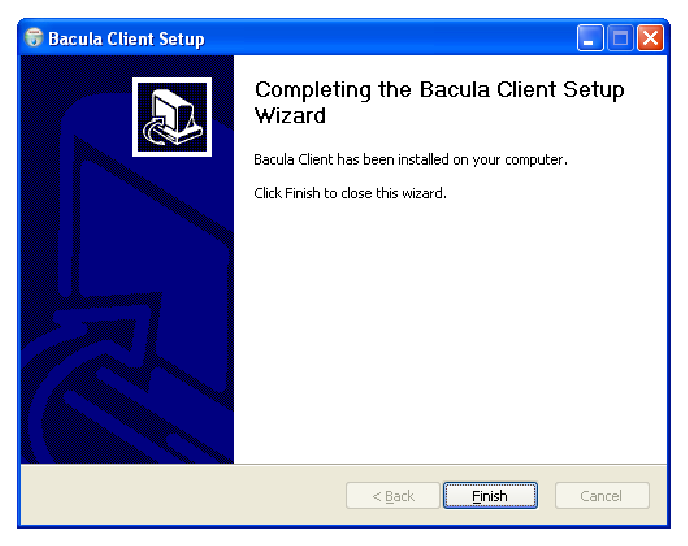
\includegraphics{./win32-finish.eps}  

\ 
\end{itemize}

That should complete the installation process. When the Bacula File Server is
ready to serve files, an icon 
\includegraphics{./idle.eps} representing a
cassette (or tape) will appear in the system tray

\includegraphics{./tray-icon.eps}; right click on it and a menu will appear.
\ 
\ \ \ \ 
\includegraphics{./menu.eps}
The {\bf Events} item is currently unimplemented, by selecting the {\bf
Status} item, you can verify whether any jobs are running or not. 

When the Bacula File Server begins saving files, the color of the holes in the
cassette icon will change from white to green 
\includegraphics{./running.eps},
and if there is an error, the holes in the cassette icon will change to red

\includegraphics{./error.eps}. 

If you are using remote desktop connections between your windows boxes, be
warned that that tray icon does not always appear. It will always be visible
when you log into the console, but the remote desktop may not display it. 

\subsubsection*{Post Win32 Installation}
\index[general]{Post Win32 Installation }
\index[general]{Win32!Post Installation }
\addcontentsline{toc}{subsubsection}{Post Win32 Installation}

After installing Bacula and before running it, you should check the contents
of {\bf
c:\textbackslash{}bacula\textbackslash{}bin\textbackslash{}bacula-fd.conf} to
ensure that it corresponds to your configuration. 

\subsubsection*{Uninstalling Bacula on Win32}
\index[general]{Win32!Uninstalling Bacula }
\index[general]{Uninstalling Bacula on Win32 }
\addcontentsline{toc}{subsubsection}{Uninstalling Bacula on Win32}

Once Bacula has been installed, it can be uninstalled using the standard
Windows Add/Remove Programs dialog found on the Control panel. 

\subsubsection*{Dealing with Win32 Problems}
\label{problems}
\index[general]{Win32!Dealing with Problems }
\index[general]{Dealing with Win32 Problems }
\addcontentsline{toc}{subsubsection}{Dealing with Win32 Problems}

The most likely source of problems is authentication when the Director
attempts to connect to the File daemon that you installed. This can occur if
the names and the passwords defined in the File daemon's configuration file
{\bf
c:\textbackslash{}bacula\textbackslash{}bin\textbackslash{}bacula-fd.conf} on
the Windows machine do not match with the names and the passwords in the
Director's configuration file {\bf bacula-dir.conf} located on your Unix/Linux
server. 

More specifically, the password found in the {\bf Client} resource in the
Director's configuration file must be the same as the password in the {\bf
Director} resource of the File daemon's configuration file. In addition, the
name of the {\bf Director} resource in the File daemon's configuration file
must be the same as the name in the {\bf Director} resource of the Director's
configuration file. 

It is a bit hard to explain in words, but if you understand that a Director
normally has multiple Clients and a Client (or File daemon) may permit access
by multiple Directors, you can see that the names and the passwords on both
sides must match for proper authentication. 

One user had serious problems with the configuration file until he realized
that the Unix end of line conventions were used and Bacula wanted them in
Windows format. This has not been confirmed though. 

Running Unix like programs on Windows machines is a bit frustrating because
the Windows command line shell (DOS Window) is rather primitive. As a
consequence, it is not generally possible to see the debug information and
certain error messages that Bacula prints. With a bit of work, however, it is
possible. When everything else fails and you want to {\bf see} what is going
on, try the following: 

\footnotesize
\begin{verbatim}
   Start a DOS shell Window.
   cd c:\bacula\bin
   bacula-fd -t >out
   type out
\end{verbatim}
\normalsize

The {\bf -t} option will cause Bacula to read the configuration file, print
any error messages and then exit. the {\bf \gt{}} redirects the output to the
file named {\bf out}, which you can list with the {\bf type} command. 

If something is going wrong later, or you want to run {\bf Bacula} with a
debug option, you might try starting it as: 

\footnotesize
\begin{verbatim}
   bacula-fd -d 100 >out
\end{verbatim}
\normalsize

In this case, Bacula will run until you explicitly stop it, which will give
you a chance to connect to it from your Unix/Linux server. In later versions
of Bacula (1.34 on, I think), when you start the File daemon in debug mode it
can write the output to a trace file {\bf bacula.trace} in the current
directory. To enable this, before running a job, use the console, and enter: 

\footnotesize
\begin{verbatim}
   trace on
\end{verbatim}
\normalsize

then run the job, and once you have terminated the File daemon, you will find
the debug output in the {\bf bacula.trace} file. 

In addition, you should look in the System Applications log on the Control
Panel to find any Windows errors that Bacula got during the startup process. 

Finally, due to the above problems, when you turn on debugging, and specify
trace=1 on a setdebug command in the Console, Bacula will write the debug
information to the file {\bf bacula.trace} in the directory from which Bacula
is executing. 

\label{Compatibility}

\subsubsection*{Windows Compatibility Considerations}
\index[general]{Windows Compatibility Considerations }
\index[general]{Considerations!Windows Compatibility }
\addcontentsline{toc}{subsubsection}{Windows Compatibility Considerations}

If any applications are running during the backup and they have files
opened exclusively, Bacula will not be able to backup those files, so be
sure you close your applications (or tell your users to close their
applications) before the backup.  Most Microsoft applications do not open
files exclusively so that they can be backed up.  However, you will need to
experiment.  In any case, if Bacula cannot open the file, it will print an
error message, so you will always know which files were not backed up.

During backup, Bacula doesn't know about the system registry, so you will
either need to write it out to an ASCII file using {\bf regedit~~/e} or use a
program specifically designed to make a copy or backup the registry. 

In Bacula version 1.31 and later, we use Windows backup API calls by
default.  Typical of Windows, programming these special BackupRead and
BackupWrite calls is a real nightmare of complications.  The end result
gives some distinct advantages and some disadvantages.

First, the advantages are that on WinNT/2K/XP systems, the security and
ownership information is now backed up.  In addition, with the exception of
files in exclusive use by another program (a major disaster for backup
programs on Windows), Bacula can now access all system files.  This means
that when you restore files, the security and ownership information will be
restored on WinNT/2K/XP along with the data.

The disadvantage of the Windows backup API calls is that it produces
non-portable backups.  That is files and their data that are backed up on
WinNT using the native API calls (BackupRead/BackupWrite) cannot be
restored on Win95/98/Me or Unix systems.  In principle, a file backed up on
WinNT can be restored on WinXP, but this remains to be seen in practice
(not yet tested).  In addition, the stand-alone tools such as {\bf bls} and
{\bf bextract} cannot be used to retrieve the data for those files because
those tools are not available on Windows.  All restores must use the Bacula
{\bf restore} command.  This restriction is mentioned for completeness, but
in practice should not create any problems.

As a default, Bacula backs up Windows systems using the Windows API calls.
If you want to backup data on a WinNT/2K/XP system and restore it on a
Unix/Win95/98/Me system, we have provided a special {\bf portable} option
that backups the data in a portable fashion by using portable API calls.
See the \ilink{portable option}{portable} on the Include statement in a
FileSet resource in the Director's configuration chapter for the details on
setting this option.  However, using the portable option means you may have
permissions problems accessing files, and none of the security and
ownership information will be backed up or restored.  The file data can,
however, be restored on any system.

You should always be able to restore any file backed up on Unix or Win95/98/Me
to any other system. On some systems, such as WinNT/2K/XP, you may have to
reset the ownership of such restored files. Any file backed up on WinNT/2K/XP
should in principle be able to be restored to a similar system (i.e.
WinNT/2K/XP), however, I am unsure of the consequences if the owner
information and accounts are not identical on both systems. Bacula will not
let you restore files backed up on WinNT/2K/XP to any other system (i.e. Unix
Win95/98/Me) if you have used the defaults. 

Finally, if you specify the {\bf portable=yes} option on the files you back
up. Bacula will be able to restore them on any other system. However, any
WinNT/2K/XP specific security and ownership information will be lost. 

The following matrix will give you an idea of what you can expect. Thanks to
Marc Brueckner for doing the tests: 

+ 

\addcontentsline{lot}{table}{WinNT/2K/XP Restore Portability Status}
\begin{longtable}{|l|l|p{2.8in}|}
 \hline 
\multicolumn{1}{|c| }{\bf Backup OS } & \multicolumn{1}{c| }{\bf Restore OS }
& \multicolumn{1}{c| }{\bf Results  } \\
 \hline {WinMe } & {WinMe } & {Works  } \\
 \hline {WinMe } & {WinNT } & {Works (SYSTEM permissions)  } \\
 \hline {WinMe } & {WinXP } & {Works (SYSTEM permissions)  } \\
 \hline {WinMe } & {Linux } & {Works (SYSTEM permissions)  } \\
 \hline {\ } & {\ } & {\  } \\
 \hline {WinXP } & {WinXP } & {Works  } \\
 \hline {WinXP } & {WinNT } & {Works (all files OK, but got ``The data is invalid''
message)  } \\
 \hline {WinXP } & {WinMe } & {Error: Win32 data stream not supported.  } \\
 \hline {WinXP } & {WinMe } & {Works if {\bf Portable=yes} specified during backup.} \\
 \hline {WinXP } & {Linux } & {Error: Win32 data stream not supported.  } \\
 \hline {WinXP } & {Linux } & {Works if {\bf Portable=yes} specified during backup.}\\
 \hline {\ } & {\ } & {\  } \\
 \hline {WinNT } & {WinNT } & {Works  } \\
 \hline {WinNT } & {WinXP } & {Works  } \\
 \hline {WinNT } & {WinMe } & {Error: Win32 data stream not supported.  } \\
 \hline {WinNT } & {WinMe } & {Works if {\bf Portable=yes} specified during backup.}\\
 \hline {WinNT } & {Linux } & {Error: Win32 data stream not supported.  } \\
 \hline {WinNT } & {Linux } & {Works if {\bf Portable=yes} specified during backup.  }\\
 \hline {\ } & {\ } & {\  } \\
 \hline {Linux } & {Linux } & {Works  } \\
 \hline {Linux } & {WinNT } & {Works (SYSTEM permissions)  } \\
 \hline {Linux } & {WinMe } & {Works  } \\
 \hline {Linux } & {WinXP } & {Works (SYSTEM permissions) }
\\ \hline 

\end{longtable}

\subsubsection*{Windows Firewalls}
\index[general]{Firewalls!Windows }
\index[general]{Windows Firewalls }
\addcontentsline{toc}{subsubsection}{Windows Firewalls}

If you turn on the firewalling feature on Windows (default in WinXP SR2), you
are likely to find that the Bacula ports are blocked and you cannot
communicated to the other daemons. This can be deactivated through the {\bf
Security Notification} dialog, which is apparently somewhere in the {\bf
Security Center}. I don't have this on my computer, so I cannot give the exact
details. 

The command: 

\footnotesize
\begin{verbatim}
netsh firewall set opmode disable
\end{verbatim}
\normalsize

is purported to disable the firewall, but this command is not accepted on my
WinXP Home machine. 

\subsubsection*{Windows Port Usage}
\index[general]{Windows Port Usage }
\index[general]{Usage!Windows Port }
\addcontentsline{toc}{subsubsection}{Windows Port Usage}

If you want to see if the File daemon has properly opened the port and is
listening, you can enter the following command in a shell window: 

\footnotesize
\begin{verbatim}
   netstat -an | findstr 910[123]
\end{verbatim}
\normalsize

\subsubsection*{Windows Disaster Recovery}
\index[general]{Recovery!Windows Disaster }
\index[general]{Windows Disaster Recovery }
\addcontentsline{toc}{subsubsection}{Windows Disaster Recovery}

We don't currently have a good solution for disaster recovery on Windows as we
do on Linux. The main piece lacking is a Windows boot floppy or a Windows boot
CD. Microsoft releases a Windows Pre-installation Environment ({\bf WinPE})
that could possibly work, but we have not investigated it. This means that
until someone figures out the correct procedure, you must restore the OS from
the installation disks, then you can load a Bacula client and restore files.
Please don't count on using {\bf bextract} to extract files from your backup
tapes during a disaster recovery unless you have backed up those files using
the {\bf portable} option. {\bf bextract} does not run on Windows, and the
normal way Bacula saves files using the Windows API prevents the files from
being restored on a Unix machine. Once you have an operational Windows OS
loaded, you can run the File daemon and restore your user files. 

Please see 
\ilink{ Disaster Recovery of Win32 Systems}{Win3233} for the latest
suggestion, which looks very promising. 

It looks like Bart PE Builder, which creates a Windows PE (Pre-installation
Environment) Boot-CD, may be just what is needed to build a complete disaster
recovery system for Win32. This distribution can be found at 
\elink{http://www.nu2.nu/pebuilder/ }{http://www.nu2.nu/pebuilder/}. 

\subsubsection*{Windows Ownership and Permissions Problems}
\index[general]{Problems!Windows Ownership and Permissions }
\index[general]{Windows Ownership and Permissions Problems }
\addcontentsline{toc}{subsubsection}{Windows Ownership and Permissions
Problems}

If you restore files backed up from WinNT/XP/2K to an alternate directory,
Bacula may need to create some higher level directories that were not saved
(or restored). In this case, the File daemon will create them under the SYSTEM
account because that is the account that Bacula runs under as a service. As of
version 1.32f-3, Bacula creates these files with full access permission.
However, there may be cases where you have problems accessing those files even
if you run as administrator. In principle, Microsoft supplies you with the way
to cease the ownership of those files and thus change the permissions.
However, a much better solution to working with and changing Win32 permissions
is the program {\bf SetACL}, which can be found at 
\elink{http://setacl.sourceforge.net/ }{http://setacl.sourceforge.net/}. 

\subsubsection*{Manually resetting the Permissions}
\index[general]{Manually resetting the Permissions }
\index[general]{Permissions!Manually resetting the }
\addcontentsline{toc}{subsubsection}{Manually resetting the Permissions}

The following solution was provided by Dan Langille \lt{}dan at langille in
the dot org domain\gt{}. The steps are performed using Windows 2000 Server but
they should apply to most Win32 platforms. The procedure outlines how to deal
with a problem which arises when a restore creates a top-level new directory.
In this example, ``top-level'' means something like {\bf
c:\textbackslash{}src}, not {\bf c:\textbackslash{}tmp\textbackslash{}src}
where {\bf c:\textbackslash{}tmp} already exists. If a restore job specifies /
as the {\bf Where:} value, this problem will arise. 

The problem appears as a directory which cannot be browsed with Windows
Explorer. The symptoms include the following message when you try to click on
that directory: 


\includegraphics{./access-is-denied.eps} 

If you encounter this message, the following steps will change the permissions
to allow full access. 

\begin{enumerate}
\item right click on the top level directory (in this example, {\bf c:/src})
   and  select {\bf Properties}. 
\item click on the Security tab. 
\item If the following message appears, you can ignore it, and click on {\bf
   OK}. 


\includegraphics{./view-only.eps} 

You should see something like this: 

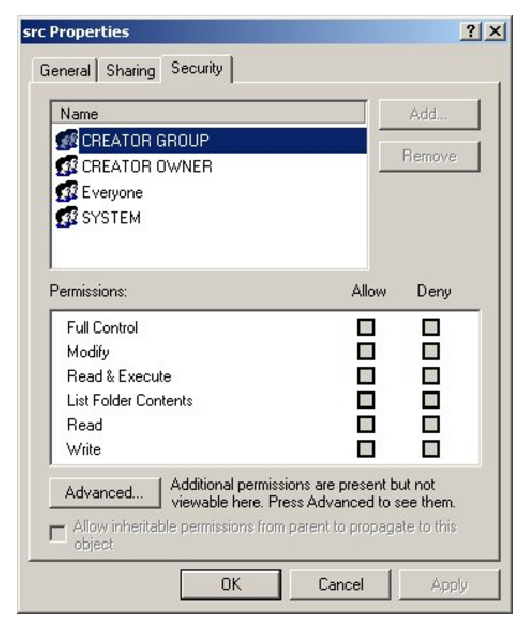
\includegraphics{./properties-security.eps} 
\item click on Advanced 
\item click on the Owner tab 
\item Change the owner to something other than the current owner (which is
   {\bf SYSTEM} in this example as shown below). 

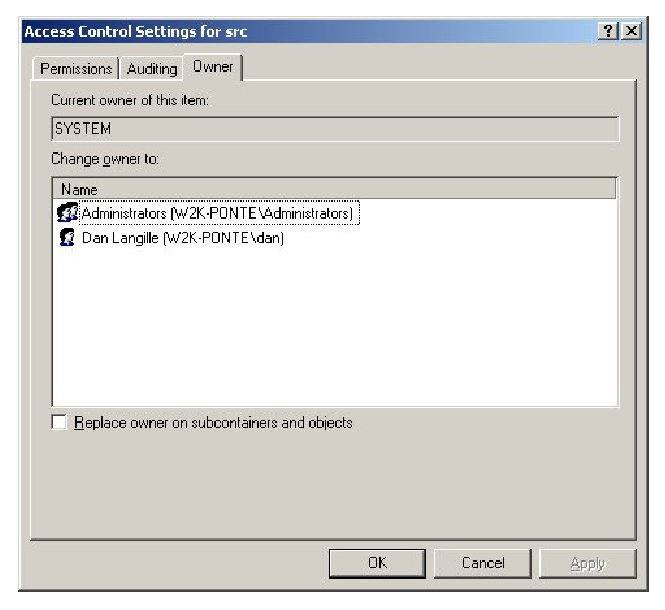
\includegraphics{./properties-security-advanced-owner.eps} 
\item ensure the ``Replace owner on subcontainers and objects'' box is 
   checked 
\item click on OK 
\item When the message ``You do not have permission to read the contents of
   directory ''c:\textbackslash{}src\textbackslash{}basis. Do you wish to replace
   the directory permissions with permissions granting you Full Control?``, click
on Yes. 

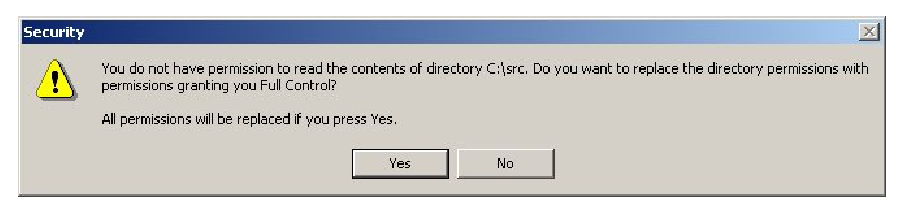
\includegraphics{./confirm.eps} 
\item Click on OK to close the Properties tab 
   \end{enumerate}

With the above procedure, you should now have full control over your restored
directory. 

\subsubsection*{Backing Up the WinNT/XP/2K System State}
\index[general]{State!Backing Up the WinNT/XP/2K System }
\index[general]{Backing Up the WinNT/XP/2K System State }
\addcontentsline{toc}{subsubsection}{Backing Up the WinNT/XP/2K System State}

A suggestion by Damian Coutts using Microsoft's NTBackup utility in
conjunction with Bacula should permit a full restore of any damaged system
files on Win2K/XP. His suggestion is to do an NTBackup of the critical system
state prior to running a Bacula backup with the following command: 

\footnotesize
\begin{verbatim}
ntbackup backup systemstate /F c:\systemstate.bkf
\end{verbatim}
\normalsize

The {\bf backup} is the command, the {\bf systemstate} says to backup only the
system state and not all the user files, and the {\bf /F
c:\textbackslash{}systemstate.bkf} specifies where to write the state file.
this file must then be saved and restored by Bacula. 

To restore the system state, you first reload a base operating system if the
OS is damaged, otherwise, this is not necessary, then you would use Bacula to
restore all the damaged or lost user's files and to recover the {\bf
c:\textbackslash{}systemstate.bkf} file. Finally if there are any damaged or
missing system files or registry problems, you run {\bf NTBackup} and {\bf
catalogue} the system statefile, and then select it for restore. The
documentation says you can't run a command line restore of the systemstate. 

To the best of my knowledge, this has not yet been tested. If you test it,
please report your results to the Bacula email list. 

\subsubsection*{Windows Considerations for Filename Specifications}
\index[general]{Specifications!Windows Considerations for Filename }
\index[general]{Windows Considerations for Filename Specifications }
\addcontentsline{toc}{subsubsection}{Windows Considerations for Filename
Specifications}

Please see the 
\ilink{Director's Configuration chapter}{win32} of this manual
for important considerations on how to specify Windows paths in Bacula FileSet
Include and Exclude directives. 

\subsubsection*{Command Line Options Specific to the Bacula Windows File
Daemon (Client)}
\index[general]{Client!Command Line Options Specific to the Bacula Windows
File Daemon }
\index[general]{Command Line Options Specific to the Bacula Windows File
Daemon (Client) }
\addcontentsline{toc}{subsubsection}{Command Line Options Specific to the
Bacula Windows File Daemon (Client)}

These options are not normally seen or used by the user, and are documented
here only for information purposes. At the current time, to change the default
options, you must either manually run {\bf Bacula} or you must manually edit
the system registry and modify the appropriate entries. 

In order to avoid option clashes between the options necessary for {\bf
Bacula} to run on Windows and the standard Bacula options, all Windows
specific options are signaled with a forward slash character (/), while as
usual, the standard Bacula options are signaled with a minus (-), or a minus
minus (\verb{--{). All the standard Bacula options can be used on the Windows
version. In addition, the following Windows only options are implemented: 

\begin{description}

\item [/servicehelper ]
   \index[fd]{/servicehelper }
   Run the service helper application  (don't use this it is deprecated.).  

\item [/service ]
   \index[fd]{/service }
   Start Bacula as a service 

\item [/run ]
   \index[fd]{/run }
   Run the Bacula application  

\item [/install ]
   \index[fd]{/install }
   Install Bacula as a service in the system registry  

\item [/remove ]
   \index[fd]{/remove }
   Uninstall Bacula from the system registry  

\item [/about ]
   \index[fd]{/about }
   Show the Bacula about dialogue box  

\item [/status ]
   \index[fd]{/status }
   Show the Bacula status dialogue box  

\item [/events ]
   \index[fd]{/events }
   Show the Bacula events dialogue box (not  yet implemented)  

\item [/kill ]
   \index[fd]{/kill }
   Stop any running {\bf Bacula}  

\item [/help ]
   \index[fd]{/help }
   Show the Bacula help dialogue box 
\end{description}

It is important to note that under normal circumstances the user should never
need to use these options as they are normally handled by the system
automatically once Bacula is installed. However, you may note these options in
some of the .bat files that have been created for your use. 

\subsubsection*{Shutting down Windows Systems}
\index[general]{Shutting down Windows Systems }
\index[general]{Systems!Shutting down Windows }
\addcontentsline{toc}{subsubsection}{Shutting down Windows Systems}

Some users like to shutdown their windows machines after a backup using a
Client Run After Job directive. If you want to do something similar, you might
take the shutdown program from the 
\elink{apcupsd project}{http://www.apcupsd.com} or one from the 
\elink{ Sysinternals
project}{http://www.sysinternals.com/ntw2k/freeware/psshutdown.shtml}. 

%%
%%

\section*{Disaster Recovery Using Bacula}
\label{_ChapterStart38}
\index[general]{Disaster Recovery Using Bacula }
\index[general]{Bacula!Disaster Recovery Using }
\addcontentsline{toc}{section}{Disaster Recovery Using Bacula}

\subsection*{General}
\index[general]{General }
\addcontentsline{toc}{subsection}{General}

When disaster strikes, you must have a plan, and you must have prepared in
advance otherwise the work of recovering your system and your files will be
considerably greater. For example, if you have not previously saved the
partitioning information for your hard disk, how can you properly rebuild it
if the disk must be replaced? 

Unfortunately, many of the steps one must take before and immediately after a
disaster are very operating system dependent. As a consequence, this chapter
will discuss in detail disaster recovery (also called Bare Metal Recovery) for
{\bf Linux} and {\bf Solaris}. For Solaris, the procedures are still quite
manual. For FreeBSD the same procedures may be used but they are not yet
developed. For Win32, no luck. Apparently an ``emergency boot'' disk allowing
access to the full system API without interference does not exist. 
\label{considerations1}

\subsection*{Important Considerations}
\index[general]{Important Considerations }
\index[general]{Considerations!Important }
\addcontentsline{toc}{subsection}{Important Considerations}

Here are a few important considerations concerning disaster recovery that you
should take into account before a disaster strikes. 

\begin{itemize}
\item If the building which houses your computers burns down or is otherwise 
   destroyed, do you have off-site backup data? 
\item Disaster recovery is much easier if you have several machines. If  you
   have a single machine, how will you handle unforeseen events  if your only
   machine is down? 
\item Do you want to protect your whole system and use Bacula to  recover
   everything? or do you want to try to restore your system from  the original
   installation disks and apply any other updates and  only restore user files? 
\end{itemize}

\label{steps1}

\subsection*{Steps to Take Before Disaster Strikes}
\index[general]{Steps to Take Before Disaster Strikes }
\index[general]{Strikes!Steps to Take Before Disaster }
\addcontentsline{toc}{subsection}{Steps to Take Before Disaster Strikes}

\begin{itemize}
\item Create a Bacula Rescue CDROM for each of your Linux systems. Note,  it
   is possible to create one CDROM by copying the bacula-hostname  directory from
   each machine to the machine where you will be  burning the CDROM.  
\item Ensure that you always have a valid bootstrap file for your  backup that
   is saved to an alternate machine. This will permit  you to easily do a full
   restore of your system. 
\item If possible copy your catalog nightly to an alternate machine.  If you
   have a valid bootstrap file, this is not necessary, but  can be very useful if
   you do not want to reload everything. .  
\item Ensure that you always have a valid bootstrap file for your  catalog
   backup that is saved to an alternate machine. This will  permit you to restore
   your catalog more easily if needed.  
\item Test using the Bacula Rescue CDROM before you are forced to use  it in
   an emergency situation. 
   \end{itemize}

\label{rescueCDROM}

\subsection*{Bare Metal Recovery on Linux with a Bacula Rescue CDROM}
\index[general]{Bare Metal Recovery on Linux with a Bacula Rescue CDROM }
\index[general]{CDROM!Bare Metal Recovery on Linux with a Bacula Rescue }
\addcontentsline{toc}{subsection}{Bare Metal Recovery on Linux with a Bacula
Rescue CDROM}

The remainder of this section concerns recovering a {\bf Linux} computer, and
parts of it relate to the Red Hat version of Linux. The {\bf Solaris}
procedures can be found below under the 
\ilink{Solaris Bare Metal Recovery}{solaris} section of this
chapter. 

If you wish to use a floppy for restoration, please see the chapter 
\ilink{Bare Metal Floppy Recovery on Linux with a Bacula Floppy Rescue
Disk}{_ChapterStart24}, but be aware that the Bacula floppy disk is deprecated
and replaced by the CDROM rescue described in this chapter. 

A so called ``Bare Metal'' recovery is one where you start with an empty hard
disk and you restore your machine. There are also cases where you may lose a
file or a directory and want it restored. Please see the previous chapter for
more details for those cases. 

Bare Metal Recovery assumes that you have the following items for your system:

\begin{itemize}
\item A Bacula Rescue CDROM containing a copy of your OS and  a copy of your
   hard disk information, as well as a  statically linked version of the Bacula
   File daemon. This chapter describes how to build such a CDROM.
\item A full Bacula backup of your system possibly including  Incremental or
   Differential backups since the last Full  backup 
\item A second system running the Bacula Director, the Catalog,  and the
   Storage daemon. (this is not an absolute requirement,  but how to get around
   it is not yet documented here) 
\end{itemize}

\subsection*{Requirements}
\index[general]{Requirements }
\addcontentsline{toc}{subsection}{Requirements}

In addition, to the above assumptions, the following conditions or
restrictions apply: 

\begin{itemize}
\item Linux only -- tested only on Red Hat, but should work on other Linuxes  
\item The scripts handle only SCSI and IDE disks  
\item All partitions will be recreated, but only {\bf ext2},  {\bf ext3}, {\bf
   rfs} and {\bf swap} partitions will be reformatted.  Any other partitions such
   as Windows FAT partitions will  not be formatted by the scripts, but you can
   do it by hand  
\item You are using either {\bf lilo} or {\bf grub} as a boot  loader, and you
   know which one (not automatically detected)  
\item The partitioning and reformating scripts will *should* work with RAID 
   devices, but probably not with other ``complicated'' disk 
   partitioning/formating schemes. They also should work with  Reiser
   filesystems. Please check them carefully. You  will probably need to edit the
   scripts by hand to make them work.  
\item You will need mkisofs (might be part of cdrtools, but is a separate rpm 
   on my system); cdrecord or some other tool for burning the CDROM. 
   \end{itemize}

\subsection*{Directories}
\index[general]{Directories }
\addcontentsline{toc}{subsection}{Directories}

To build the Bacula Rescue CDROM, you will find the necessary scripts in {\bf
rescue/linux/cdrom} subdirectory of the Bacula source code. If you installed
the bacula-rescue rpm package the scripts will be found in the {\bf
/etc/bacula/rescue/cdrom} directory. 

\subsection*{Preparation for a Bare Metal Recovery}
\index[general]{Recovery!Preparation for a Bare Metal }
\index[general]{Preparation for a Bare Metal Recovery }
\addcontentsline{toc}{subsection}{Preparation for a Bare Metal Recovery}

Before you can do a Bare Metal recovery, you must create a Bacula Rescue
CDROM, which will contain everything you need to begin recovery. This assumes
that you will have your Directory and Storage daemon running on a different
machine. If you want to recover a machine where the Director and/or the
database were previously running things will be much more complicated. 

\subsection*{Creating a Bacula Rescue CDROM}
\index[general]{CDROM!Creating a Bacula Rescue }
\index[general]{Creating a Bacula Rescue CDROM }
\addcontentsline{toc}{subsection}{Creating a Bacula Rescue CDROM}

The primary goals of the Bacula rescue CD are: 

\begin{itemize}
\item NOT to be a general or universal recovery disk. 
\item to capture and setup a restore environment for a  single system running
   as a Client. 
\item to capture the current state of the hard disks on your system, so that
   they can be easily restored from pre-generated  scripts. Note, this is
   not done by any other rescue CDROM, as far as I am aware.
\item to create and save a statically linked copy of your  current Bacula FD. 
   Thus you need no packages or other software to be installed before using
   this CDROM and the Bacula File daemon on it.
\item to be relatively easy to create. In most cases  you simply type {\bf
   make all} in the {\bf rescue/linux/cdrom}  directory, then burn the ISO image
   created. In contrast,  if you have looked at  any of the documentation on how
   to remaster a CD or how to roll your  own, your head will spin (at least mine
   did). 
\item to be easy for you to add any additional files, binaries,  or libraries
   to the CD. 
\item to build and work on any (or almost any) Linux  flavor or release. 
\item you might ask why I don't use Knoppix or some other preprepared recovery
   disk, especially since Knoppix is very kind and provides the Bacula FD on
   their disk.  The answer is that: I am more comfortable having my Linux boot
   up in rescue mode rather than another flavor. In addition, the Bacula rescue
   CDROM contains a complete snapshot of your disk partitioning, which is not
   the case with any other rescue disk. If your harddisk dies, do you remember all
   the partitions you had and how big they are?  I don't, and without that information,
   you have little hope of reformatting your harddisk and rebuilding your system.
\end{itemize}

One of the main of the advantages of a Bacula Rescue CDROM is that it contains
a bootable copy of your system, so you should be familiar with it. 

You should probably make a new rescue CDROM each time you make any major
updates to your kernel, and every time you upgrade a major version of Bacula. 

The whole process with the exception of burning the CDROM is done with the
following commands: 

\footnotesize
\begin{verbatim}
(Build a working version of Bacula in the
 bacula-source directory)
cd <bacula-source>
./configure (your options)
make
cd <bacula-source>/rescue/linux/cdrom
su (become root)
make all
\end{verbatim}
\normalsize

For users of the bacula-rescue rpm the static bacula-fd has already been built
and placed in {\bf /etc/bacula/rescue/cdrom/bin/} along with a symbolic link
to your {\bf /etc/bacula/bacula-fd.conf} file. Rpm users only need to do the
second step: 

\footnotesize
\begin{verbatim}
cd /etc/bacula/rescue/cdrom
su (become root)
make all
\end{verbatim}
\normalsize

At this point, if the scripts are successful, they should have done the
following things: 

\begin{itemize}
\item Made a copy of your kernel and its essential files.  
\item Copied a number of binary files from your system.  
\item Copied all the necessary shared libraries to run the above  binary
   files.  
\item Made a statically-linked version of your File daemon and  copied it into
   the CDROM build area.  
\item Made an ISO image and left it in {\bf bootcd.iso} 
   \end{itemize}

Once this is accomplished, you need only burn it into a CDROM. This can be
done directly from the makefile with: 

\footnotesize
\begin{verbatim}
make burn
\end{verbatim}
\normalsize

However, you may need to modify the Makefile to properly specify your CD
burner as the detection process is complicated especially if you have two
CDROMs or do not have {\bf cdrecord} loaded on your system. Users of the
rescue rpm package should definitely examine the Makefile since it was
configured on the host used to produce the rpm package. If you find that the
{\bf make burn} does not work for you, try doing a: 

\footnotesize
\begin{verbatim}
make scan
\end{verbatim}
\normalsize

and use the output of that to modify the Makefile accordingly. 

The ``make all'' that you did above actually does the equivalent to the
following: 

\footnotesize
\begin{verbatim}
make kernel
make binaries
make bacula
make iso
\end{verbatim}
\normalsize

If you wish, you can modify what you put on the CDROM and redo any part of the
make that you wish. For example, if you want to add a new directory, you might
do the first three makes, then add a new directory to the CDROM, and finally
do a ``make iso''. Please see the README file in the {\bf rescue/linux/cdrom}
or {\bf /etc/bacula/rescue/cdrom}directory for instructions on changing the
contents of the CDROM. 

At the current time, the size of the CDROM is about 50MB (compressed to about
20MB), so there is quite a bit more room for additional program. Keep in mind
that when this CDROM is booted, *everything* is in memory, so the total size
cannot exceed your memory size, and even then you will need some reserve
memory for running programs, ... 
\label{twosystemcd}

\subsection*{Putting Two or More Systems on Your Rescue Disk}
\index[general]{Putting Two or More Systems on Your Rescue Disk }
\index[general]{Disk!Putting Two or More Systems on Your Rescue }
\addcontentsline{toc}{subsection}{Putting Two or More Systems on Your Rescue
Disk}

You can put multiple systems on the same rescue CD if you wish. This is
because the information that is specific to your OS will be stored in the {\bf
/bacula-hostname} directory, where {\bf hostname} is the name of the host on
which you are building the CD. Suppose for example, you have two systems. One
named {\bf client1} and one named {\bf client2}. Assume also that your CD
burner is on client1, and that is the machine we start on, and that we can ssh
into client2 and also client2's disks are mounted on client1. 

\footnotesize
\begin{verbatim}
ssh client2
cd <bacula-source>
./configure (your options)
make
cd rescue/linux/cdrom
su
(enter root password)
make bacula
exit
exit
\end{verbatim}
\normalsize

Again, for rpm package users the above command set would be: 

\footnotesize
\begin{verbatim}
ssh client2
cd /etc/bacula/rescue/cdrom
su
(enter root password)
make bacula
exit
exit
\end{verbatim}
\normalsize

Thus we have just built a Bacula rescue directory on client2. Now, on client1,
we copy the appropriate directory to two places (explained below), then build
an ISO and burn it: 

\footnotesize
\begin{verbatim}
cd <bacula-source>
./configure (your options)
make
cd rescue/linux/cdrom
su
(enter root password)
c=/mnt/client2/home/user/bacula/rescue/linux/cdrom
cp -a $c/roottree/bacula-client2 roottree
cp -a $c/roottree/bacula-client2 cdtree
make all
make burn
exit
\end{verbatim}
\normalsize

And with the rpm package: 

\footnotesize
\begin{verbatim}
cd /etc/bacula/rescue/cdrom
su
(enter root password)
c=/mnt/client2/etc/bacula/rescue/cdrom
cp -a $c/roottree/bacula-client2 roottree
cp -a $c/roottree/bacula-client2 cdtree
make all
make burn
exit
\end{verbatim}
\normalsize

In summary, with the above commands, we first build a Bacula directory on
client2 in roottree/bacula-client2, then we copied the bacula-client2
directory into the client1's roottree so it is available in memory after
booting, and we also copied it into the cdtree so it will also be on the CD as
a separate directory and thus can be read without booting the CDROM. Then we
made and burned the CDROM for client1, which of course, contains the client2
data. 
\label{restore}

\subsection*{Restoring a Client System}
\index[general]{Restoring a Client System }
\index[general]{System!Restoring a Client }
\addcontentsline{toc}{subsection}{Restoring a Client System}

Now, let's assume that your hard disk has just died and that you have replaced
it with an new identical drive. In addition, we assume that you have: 

\begin{enumerate}
\item A recent Bacula backup (Full plus Incrementals)  
\item A Bacula Rescue CDROM.  
\item Your Bacula Director, Catalog, and Storage daemon running  on another
   machine on your local network. 
   \end{enumerate}

This is a relatively simple case, and later in this chapter, as time permits,
we will discuss how you might recover from a situation where the machine that
crashes is your main Bacula server (i.e. has the Director, the Catalog, and
the Storage daemon). 

You will take the following steps to get your system back up and running: 

\begin{enumerate}
\item Boot with your Bacula Rescue CDROM.  
\item Start the Network (local network)  
\item Re-partition your hard disk(s) as it was before  
\item Re-format your partitions  
\item Restore the Bacula File daemon (static version)  
\item Perform a Bacula restore of all your files  
\item Re-install your boot loader  
\item Reboot 
   \end{enumerate}

Now for the details ... 

\subsection*{Boot with your Bacula Rescue CDROM}
\index[general]{CDROM!Boot with your Bacula Rescue }
\index[general]{Boot with your Bacula Rescue CDROM }
\addcontentsline{toc}{subsection}{Boot with your Bacula Rescue CDROM}

When the CDROM boots, you will be presented with a script that looks like: 

\footnotesize
\begin{verbatim}
 
      Welcome to the Bacula Rescue Disk 1.1.0
To proceed, press the <ENTER> key or type "linux <runlevel>"
 
   linux 1     -> shell
   linux 2     -> login  (default if ENTER pressed)
   linux 3     -> network started and login (network not working yet)
   linux debug -> print debug during boot then login
\end{verbatim}
\normalsize

Normally, at this point, you simply press ENTER. However, you may supply
options for the boot if you wish. 

Once it has booted, you will be requested to login something like: 

\footnotesize
\begin{verbatim}
Welcome to the Bacula Rescue CDROM
2.4.21-15.0.4.EL #1 Wed Aug 4 03:08:03 EDT 2004
Please login using root and your root password ...
RescueCD login:
\end{verbatim}
\normalsize

Note, you must enter the root password for the system on which you loaded the
kernel or on which you did the build of the CDROM. Once you are logged in,
your will be in the home directory for {\bf root}, and you can proceed to
examine your system. 

The complete Bacula rescue part of the CD will be in the directory: {\bf
/bacula-hostname}, where hostname is replaced by the name of the host machine
on which you did the build for the CDROM. This naming procedure allows you to
put multiple restore environments for each of your machines on a single CDROM
if you so wish to do. Please see the README document in the {\bf
rescue/linux/cdrom} directory for more information on adding to the CDROM. 

\paragraph*{Start the Network:}

At this point, you should bring up your network. Normally, this is quite
simple and requires just a few commands. Please cd into the /bacula-hostname
directory before continuing. To simplify your task, we have created a script
that should work in most cases by typing: 

\footnotesize
\begin{verbatim}
cd /bacula-hostname
./start_network
\end{verbatim}
\normalsize

You can test it by pinging another machine, or pinging your broken machine
machine from another machine. Do not proceed until your network is up. 

\paragraph*{Partition Your Hard Disk(s):}

Assuming that your hard disk crashed and needs repartitioning, proceed with: 

\footnotesize
\begin{verbatim}
./partition.hda
\end{verbatim}
\normalsize

If you have multiple disks, do the same for each of them. For SCSI disks, the
repartition script will be named: {\bf partition.sda}. If the script complains
about the disk being in use, simply go back and redo the {\bf df} command and
{\bf umount} commands until you no longer have your hard disk mounted. Note,
in many cases, if your hard disk was seriously damaged or a new one installed,
it will not automatically be mounted. If it is mounted, it is because the
emergency kernel found one or more possibly valid partitions. 

If for some reason this procedure does not work, you can use the information
in {\bf partition.hda} to re-partition your disks by hand using {\bf fdisk}. 

\paragraph*{Format Your Hard Disk(s):}

If you have repartitioned your hard disk, you must format it appropriately.
The formatting script will put back swap partitions, normal Unix partitions
(ext2) and journaled partitions (ext3) as well as Reiser partitions (rei). Do
so by entering for each disk: 

\footnotesize
\begin{verbatim}
./format.hda
\end{verbatim}
\normalsize

The format script will ask you if you want a block check done. We recommend to
answer yes, but realize that for very large disks this can take hours. 

\paragraph*{Mount the Newly Formatted Disks:}

Once the disks are partitioned and formatted, you can remount them with the
{\bf mount\_drives} script. All your drives must be mounted for Bacula to be
able to access them. Run the script as follows: 

\footnotesize
\begin{verbatim}
./mount_drives
df
\end{verbatim}
\normalsize

The {\bf df} command will tell you if the drives are mounted. If not, re-run
the script again. It isn't always easy to figure out and create the mount
points and the mounts in the proper order, so repeating the {\bf
./mount\_drives} command will not cause any harm and will most likely work the
second time. If not, correct it by hand before continuing. 

\paragraph*{Restore and Start the File Daemon:}

If you have booted with a Bacula Rescue CDROM, your statically linked Bacula
File daemon and the bacula-fd.conf file with be in the /bacula-hostname/bin
directory. Make sure {\bf bacula-fd} and {\bf bacula-fd.conf} are both there. 

Edit the Bacula configuration file, create the working/pid/subsys directory if
you haven't already done so above, and start Bacula. Before starting Bacula,
you will need to move it and bacula-fd.conf from /bacula-hostname/bin, to the
/mnt/disk/tmp directory so that it will be on your hard disk. Then start it
with the following command: 

\footnotesize
\begin{verbatim}
chroot /mnt/disk /tmp/bacula-fd -c /tmp/bacula-fd.conf
\end{verbatim}
\normalsize

The above command starts the Bacula File daemon with your the proper root disk
location (i.e. {\bf /mnt/disk/tmp}. If Bacula does not start correct the
problem and start it. You can check if it is running by entering: 

\footnotesize
\begin{verbatim}
ps fax
\end{verbatim}
\normalsize

You can kill Bacula by entering: 

\footnotesize
\begin{verbatim}
kill -TERM <pid>
\end{verbatim}
\normalsize

where {\bf pid} is the first number printed in front of the first occurrence
of {\bf bacula-fd} in the {\bf ps fax} command. 

Now, you should be able to use another computer with Bacula installed to check
the status by entering: 

\footnotesize
\begin{verbatim}
status client=xxxx
\end{verbatim}
\normalsize

into the Console program, where xxxx is the name of the client you are
restoring. 

One common problem is that your {\bf bacula-dir.conf} may contain machine
addresses that are not properly resolved on the stripped down system to be
restored because it is not running DNS. This is particularly true for the
address in the Storage resource of the Director, which may be very well
resolved on the Director's machine, but not on the machine being restored and
running the File daemon. In that case, be prepared to edit {\bf
bacula-dir.conf} to replace the name of the Storage daemon's domain name with
its IP address. 

\paragraph*{Restore Your Files:}

On the computer that is running the Director, you now run a {\bf restore}
command and select the files to be restored (normally everything), but before
starting the restore, there is one final change you must make using the {\bf
mod} option. You must change the {\bf Where} directory to be the root by using
the {\bf mod} option just before running the job and selecting {\bf Where}.
Set it to: 

\footnotesize
\begin{verbatim}
/
\end{verbatim}
\normalsize

then run the restore. 

You might be tempted to avoid using {\bf chroot} and running Bacula directly
and then using a {\bf Where} to specify a destination of {\bf /mnt/disk}. This
is possible, however, the current version of Bacula always restores files to
the new location, and thus any soft links that have been specified with
absolute paths will end up with {\bf /mnt/disk} prefixed to them. In general
this is not fatal to getting your system running, but be aware that you will
have to fix these links if you do not use {\bf chroot}. 

\paragraph*{Final Step:}

At this point, the restore should have finished with no errors, and all your
files will be restored. One last task remains and that is to write a new boot
sector so that your machine will boot. For {\bf lilo}, you enter the following
command: 

\footnotesize
\begin{verbatim}
./run_lilo
\end{verbatim}
\normalsize

If you are using grub instead of lilo, you must enter the following: 

\footnotesize
\begin{verbatim}
./run_grub
\end{verbatim}
\normalsize

Note, I've had quite a number of problems with {\bf grub} because it is rather
complicated and not designed to install easily under a simplified system. So,
if you experience errors or end up unexpectedly in a {\bf chroot} shell,
simply exit back to the normal shell and type in the appropriate commands from
the {\bf run\_grub} script by hand until you get it to install. When you run
the run\_grub script, it will print the commands that you should manually
enter if that is necessary. 

\paragraph*{Reboot:}

First unmount all your hard disks, otherwise they will not be cleanly
shutdown, then reboot your machine by entering {\bf exit} until you get to the
main prompt then enter {\bf ctl-d}. Once back to the main CDROM prompt, you
will need to turn the power off then back on to your machine to get it to
reboot. 

If everything went well, you should now be back up and running. If not,
re-insert the emergency boot CDROM, boot, and figure out what is wrong. 
\label{server}

\subsection*{Restoring a Server}
\index[general]{Restoring a Server }
\index[general]{Server!Restoring a }
\addcontentsline{toc}{subsection}{Restoring a Server}

Above, we considered how to recover a client machine where a valid Bacula
server was running on another machine. However, what happens if your server
goes down and you no longer have a running Director, Catalog, or Storage
daemon? There are several solutions: 

\begin{enumerate}
\item Bring up static versions of your Director, Catalog, and Storage  daemon.

\item Move your server to another machine. 
   \end{enumerate}

The first option, is very difficult because it requires you to have created a
static version of the Director and the Storage daemon as well as the Catalog.
If the Catalog uses MySQL or PostgreSQL, this may or may not be possible. In
addition, to loading all these programs on a bare system (quite possible), you
will need to make sure you have a valid driver for your tape drive. 

The second suggestion is probably a much simpler solution, and one I have done
myself. To do so, you might want to consider the following steps: 

\begin{itemize}
\item If you are using MySQL or PostgreSQL, configure, build and install it
   from  source (or user rpms) on your new system.  
\item Load the Bacula source code onto your new system, configure,  install
   it, and create the Bacula database.  
\item If you have a valid saved Bootstrap file as created for your  damaged
   machine with WriteBootstrap, use it to restore the  files to the damaged
   machine, where you have loaded a static Bacula  File daemon using the Bacula
Rescue disk). This is done by  using the restore command and at the yes/mod/no
prompt,  selecting {\bf mod} then specifying the path to the bootstrap  file. 
\item If you have the Bootstrap file, you should now be back up and  running,
   if you do not have a Bootstrap file, continue with the  suggestions below.  
\item Using {\bf bscan} scan the last set of backup tapes into your  MySQL,
   PostgreSQL or SQLite database.  
\item Start Bacula, and using the Console {\bf restore} command,  restore the
   last valid copy of the Bacula database and the  the Bacula configuration
   files.  
\item Move the database to the correct location. 
\item Start the database, and restart Bacula. Then use  the Console {\bf
   restore} command, restore all the files  on the damaged machine, where you
   have loaded a Bacula File  daemon using the Bacula Rescue disk. 
\end{itemize}

\label{problems2}

\subsection*{Linux Problems or Bugs}
\index[general]{Bugs!Linux Problems or }
\index[general]{Linux Problems or Bugs }
\addcontentsline{toc}{subsection}{Linux Problems or Bugs}

Since every flavor and every release of Linux is different, there are likely
to be some small difficulties with the scripts, so please be prepared to edit
them in a minimal environment. A rudimentary knowledge of {\bf vi} is very
useful. Also, these scripts do not do everything. You will need to reformat
Windows partitions by hand, for example. 

Getting the boot loader back can be a problem if you are using {\bf grub}
because it is so complicated. If all else fails, reboot your system from your
floppy but using the restored disk image, then proceed to a reinstallation of
grub (looking at the run-grub script can help). By contrast, lilo is a piece
of cake. 
\label{FreeBSD1}

\subsection*{FreeBSD Bare Metal Recovery}
\index[general]{Recovery!FreeBSD Bare Metal }
\index[general]{FreeBSD Bare Metal Recovery }
\addcontentsline{toc}{subsection}{FreeBSD Bare Metal Recovery}

The same basic techniques described above also apply to FreeBSD. Although we
don't yet have a fully automated procedure, Alex Torres Molina has provided us
with the following instructions with a few additions from Jesse Guardiani and
Dan Languille: 

\begin{enumerate}
\item Boot with the FreeBSD installation disk 
\item Go to Custom, Partition and create your slices and go to Label and 
   create the particions that you want. Apply changes. 
\item Go to Fixit to start a emergency console. 
\item Create devs ad0 .. .. if don't exist under /mnt2/dev (in my  situation)
   with MAKEDEV. The device or devices you  create depend on what hard drives you
   have. ad0 is your  first ATA drive. da0 would by your first SCSI drive.  Under
OS version 5 and greater, your device files are  most likely automatically
created for you. 
\item mkdir /mnt/disk
   this is the root of the new disk 
\item mount /mnt2/dev/ad0s1a /mnt/disk
   mount /mnt2/dev/ad0s1c /mnt/disk/var
   mount /mnt2/dev/ad0s1d /mnt/disk/usr
.....
The same hard drive isssues as above apply here too.  Note, under OS version 5
or higher, your disk devices may  be in /dev not /mnt2/dev. 
\item Network configuraion (ifconfig xl0 ip/mask + route add default 
   ip-gateway) 
\item mkdir /mnt/disk/tmp 
\item cd /mnt/disk/tmp 
\item Copy bacula-fd and bacula-fd.conf to this path 
\item If you need to use sftp to copy files then you must do this:
   ln -s /mnt2/usr/bin /usr/bin 
\item chmod u+x bacula-fd 
\item Modify bacula-fd.conf to fit this machine 
\item Copy /bin/sh to /mnt/disk, neccesary for chroot 
\item Don't forget to put your bacula-dir's IP address and domain  name in
   /mnt/disk/etc/hosts if it's not on a public net.  Otherwise the FD on the
   machine you are restoring to  won't be able to contact the SD and DIR on the
remote machine. 
\item mkdir -p /mnt/disk/var/db/bacula 
\item chroot /mnt/disk /tmp/bacula-fd -c /tmp/bacula-fd.conf
   to start bacula-fd 
\item Now you can go to bacula-dir and restore the job with the entire 
   contents of the broken server. 
\item You must create /proc 
   \end{enumerate}

\label{solaris}

\subsection*{Solaris Bare Metal Recovery}
\index[general]{Solaris Bare Metal Recovery }
\index[general]{Recovery!Solaris Bare Metal }
\addcontentsline{toc}{subsection}{Solaris Bare Metal Recovery}

The same basic techniques described above apply to Solaris: 

\begin{itemize}
\item the same restrictions as those given for Linux apply  
\item you will need to create a Bacula Rescue disk 
   \end{itemize}

However, during the recovery phase, the boot and disk preparation procedures
are different: 

\begin{itemize}
\item there is no need to create an emergency boot disk  since it is an
   integrated part of the Solaris boot.  
\item you must partition and format your hard disk by hand  following manual
   procedures as described in W. Curtis Preston's  book ``Unix Backup \&
   Recovery'' 
\end{itemize}

Once the disk is partitioned, formatted and mounted, you can continue with
bringing up the network and reloading Bacula. 

\subsection*{Preparing Solaris Before a Disaster}
\index[general]{Preparing Solaris Before a Disaster }
\index[general]{Disaster!Preparing Solaris Before a }
\addcontentsline{toc}{subsection}{Preparing Solaris Before a Disaster}

As mentioned above, before a disaster strikes, you should prepare the
information needed in the case of problems. To do so, in the {\bf
rescue/solaris} subdirectory enter: 

\footnotesize
\begin{verbatim}
su
./getdiskinfo
./make_rescue_disk
\end{verbatim}
\normalsize

The {\bf getdiskinfo} script will, as in the case of Linux described above,
create a subdirectory {\bf diskinfo} containing the output from several system
utilities. In addition, it will contain the output from the {\bf SysAudit}
program as described in Curtis Preston's book. This file {\bf
diskinfo/sysaudit.bsi} will contain the disk partitioning information that
will allow you to manually follow the procedures in the ``Unix Backup \&
Recovery'' book to repartition and format your hard disk. In addition, the
{\bf getdiskinfo} script will create a {\bf start\_network} script. 

Once you have your your disks repartitioned and formatted, do the following: 

\begin{itemize}
\item Start Your Network with the {\bf start\_network} script  
\item Restore the Bacula File daemon as documented above  
\item Perform a Bacula restore of all your files using the same  commands as
   described above for Linux  
\item Re-install your boot loader using the instructions outlined  in the
   ``Unix Backup \& Recovery'' book  using installboot 
   \end{itemize}

\label{genbugs}

\subsection*{Bugs and Other Considerations}
\index[general]{Considerations!Bugs and Other }
\index[general]{Bugs and Other Considerations }
\addcontentsline{toc}{subsection}{Bugs and Other Considerations}

\paragraph*{Directory Modification and Access Times are Modified on pre-1.30
Baculas :}

When a pre-1.30 version of Bacula restores a directory, it first must create
the directory, then it populates the directory with its files and
subdirectories. The act of creating the files and subdirectories updates both
the modification and access times associated with the directory itself. As a
consequence, all modification and access times of all directories will be
updated to the time of the restore. 

This has been corrected in Bacula version 1.30 and later. The directory
modification and access times is reset to the value saved in the backup after
all the files and subdirectories have been restored. This has been tested and
verified on normal restore operations, but not verified during a bare metal
recovery. 

\paragraph*{Strange Bootstrap Files:}

If any of you look closely at the bootstrap file that is produced and used for
the restore (I sure do), you will probably notice that the FileIndex item does
not include all the files saved to the tape. This is because in some instances
there are duplicates (especially in the case of an Incremental save), and in
such circumstances, {\bf Bacula} restores only the last of multiple copies of
a file or directory. 
\label{Win3233}

\subsection*{Disaster Recovery of Win32 Systems}
\index[general]{Systems!Disaster Recovery of Win32 }
\index[general]{Disaster Recovery of Win32 Systems }
\addcontentsline{toc}{subsection}{Disaster Recovery of Win32 Systems}

Due to open system files, and registry problems, Bacula cannot save and
restore a complete Win2K/XP/NT environment. 

A suggestion by Damian Coutts using Microsoft's NTBackup utility in
conjunction with Bacula should permit a Full bare metal restore of Win2K/XP
(and possibly NT systems). His suggestion is to do an NTBackup of the critical
system state prior to running a Bacula backup with the following command: 

\footnotesize
\begin{verbatim}
ntbackup backup systemstate /F c:\systemstate.bkf
\end{verbatim}
\normalsize

The {\bf backup} is the command, the {\bf systemstate} says to backup only the
system state and not all the user files, and the {\bf /F
c:\textbackslash{}systemstate.bkf} specifies where to write the state file.
this file must then be saved and restored by Bacula. 

To restore the system state, you first reload a base operating system, then
you would use Bacula to restore all the users files and to recover the {\bf
c:\textbackslash{}systemstate.bkf} file, and finally, run {\bf NTBackup} and
{\bf catalogue} the system statefile, and then select it for restore. The
documentation says you can't run a command line restore of the systemstate. 

This procedure has been confirmed to work by Ludovic Strappazon -- many
thanks! 

A new tool is provided in the form of a bacula plugin for the BartPE rescue
CD. BartPE is a self-contained WindowsXP boot CD which you can make using the
PeBuilder tools available at 
\elink{http://www.nu2.nu/pebuilder/}{http://www.nu2.nu/pebuilder/} and a valid
Windows XP SP1 CDROM. The plugin is provided as a zip archive. Unzip the file
and copy the bacula directory into the plugin directory of your BartPE
installation. Edit the configuration files to suit your installation and build
your CD according to the instructions at Bart's site. This will permit you to
boot from the cd, configure and start networking, start the bacula file client
and access your director with the console program. The programs menu on the
booted CD contains entries to install the file client service, start the file
client service, and start the WX-Console. You can also open a command line
window and CD Programs\textbackslash{}Bacula and run the command line console
bconsole. 

\subsection*{Resetting Directory and File Ownership and Permissions on Win32
Systems}
\index[general]{Systems!Resetting Directory and File Ownership and Permissions
on Win32 }
\index[general]{Resetting Directory and File Ownership and Permissions on
Win32 Systems }
\addcontentsline{toc}{subsection}{Resetting Directory and File Ownership and
Permissions on Win32 Systems}

Bacula versions after 1.31 should properly restore ownership and permissions
on all WinNT/XP/2K systems. If you do experience problems, generally in
restores to alternate directories because higher level directories were not
backed up by Bacula, you can correct any problems with the {\bf SetACL}
available under the GPL license at: 
\elink{http://sourceforge.net/projects/setacl/}{http://sourceforge.net/project%
s/setacl/}. 

\subsection*{Alternate Disaster Recovery Suggestion for Win32 Systems}
\index[general]{Systems!Alternate Disaster Recovery Suggestion for Win32 }
\index[general]{Alternate Disaster Recovery Suggestion for Win32 Systems }
\addcontentsline{toc}{subsection}{Alternate Disaster Recovery Suggestion for
Win32 Systems}

Ludovic Strappazon has suggested an interesting way to backup and restore
complete Win32 partitions. Simply boot your Win32 system with a Linux Rescue
disk as described above for Linux, install a statically linked Bacula, and
backup any of the raw partitions you want. Then to restore the system, you
simply restore the raw partition or partitions. Here is the email that Ludovic
recently sent on that subject: 

\footnotesize
\begin{verbatim}
I've just finished testing my brand new cd LFS/Bacula
with a raw Bacula backup and restore of my portable.
I can't resist sending you the results: look at the rates !!!
hunt-dir: Start Backup JobId 100, Job=HuntBackup.2003-04-17_12.58.26
hunt-dir: Bacula 1.30 (14Apr03): 17-Apr-2003 13:14
JobId:                  100
Job:                    HuntBackup.2003-04-17_12.58.26
FileSet:                RawPartition
Backup Level:           Full
Client:                 sauvegarde-fd
Start time:             17-Apr-2003 12:58
End time:               17-Apr-2003 13:14
Files Written:          1
Bytes Written:          10,058,586,272
Rate:                   10734.9 KB/s
Software Compression:   None
Volume names(s):        000103
Volume Session Id:      2
Volume Session Time:    1050576790
Last Volume Bytes:      10,080,883,520
FD termination status:  OK
SD termination status:  OK
Termination:            Backup OK
hunt-dir: Begin pruning Jobs.
hunt-dir: No Jobs found to prune.
hunt-dir: Begin pruning Files.
hunt-dir: No Files found to prune.
hunt-dir: End auto prune.
hunt-dir: Start Restore Job RestoreFilesHunt.2003-04-17_13.21.44
hunt-sd: Forward spacing to file 1.
hunt-dir: Bacula 1.30 (14Apr03): 17-Apr-2003 13:54
JobId:                  101
Job:                    RestoreFilesHunt.2003-04-17_13.21.44
Client:                 sauvegarde-fd
Start time:             17-Apr-2003 13:21
End time:               17-Apr-2003 13:54
Files Restored:         1
Bytes Restored:         10,056,130,560
Rate:                   5073.7 KB/s
FD termination status:  OK
Termination:            Restore OK
hunt-dir: Begin pruning Jobs.
hunt-dir: No Jobs found to prune.
hunt-dir: Begin pruning Files.
hunt-dir: No Files found to prune.
hunt-dir: End auto prune.
\end{verbatim}
\normalsize

\label{running}

\subsection*{Restoring to a Running System}
\index[general]{System!Restoring to a Running }
\index[general]{Restoring to a Running System }
\addcontentsline{toc}{subsection}{Restoring to a Running System}

If for some reason you want to do a Full restore to a system that has a
working kernel, you will need to take care not to overwrite the following
files: 

\footnotesize
\begin{verbatim}
/etc/grub.conf
/etc/X11/Conf
/etc/fstab
/etc/mtab
/lib/modules
/usr/modules
/usr/X11R6
/etc/modules.conf
\end{verbatim}
\normalsize

\label{Resources}

\subsection*{Additional Resources}
\index[general]{Additional Resources }
\index[general]{Resources!Additional }
\addcontentsline{toc}{subsection}{Additional Resources}

Many thanks to Charles Curley who wrote 
\elink{ Linux Complete Backup and Recovery
HOWTO}
{http://www.tldp.org/HOWTO/Linux-Complete-Backup-and-Recovery-HOWTO/index.html%
} for the 
\elink{The Linux Documentation Project}{http://www.tldp.org/}. This is an
excellent document on how to do Bare Metal Recovery on Linux systems, and it
was this document that made me realize that Bacula could do the same thing. 

You can find quite a few additional resources, both commercial and free at 
\elink{Storage Mountain}{http://www.backupcentral.com}, formerly known as
Backup Central. 

And finally, the O'Reilly book, ``Unix Backup \& Recovery'' by W. Curtis
Preston covers virtually every backup and recovery topic including bare metal
recovery for a large range of Unix systems. 

%%
%%

\section*{Using Bacula to Encrypt Communications to Clients}
\label{_ChapterStart6}
\index[general]{Clients!Using Bacula to Encrypt Communications to }
\index[general]{Using Bacula to Encrypt Communications to Clients }
\addcontentsline{toc}{section}{Using Bacula to Encrypt Communications to
Clients}

At the current time, Bacula does not have built-in communications encryption.
However, without too much effort, it is possible to encrypt the communications
between any of the daemons. This chapter will show you how to use {\bf
stunnel} to encrypt communications to your client programs. We assume the
Director and the Storage daemon are running on one machine that will be called
{\bf server} and the Client or File daemon is running on a different machine
called {\bf client}. Although the details may be slightly different, the same
principles apply whether you are encrypting between Unix, Linux, or Win32
machines. This example was developed between two Linux machines running
stunnel version 4.04-4 on a Red Hat Enterprise 3.0 system. 

\subsection*{Communications Ports Used}
\index[general]{Used!Communications Ports }
\index[general]{Communications Ports Used }
\addcontentsline{toc}{subsection}{Communications Ports Used}

First, you must know that with the standard Bacula configuration, the Director
will contact the File daemon on port 9102. The File daemon then contacts the
Storage daemon using the address and port parameters supplied by the Director.
The standard port used will be 9103. This in the typical server/client view of
the world, the File daemon is a server to the Director (i.e. listens for the
Director to contact it), and the Storage daemon is a server to the File
daemon. 

\subsection*{Encryption}
\index[general]{Encryption }
\addcontentsline{toc}{subsection}{Encryption}

The encryption is accomplished between the Director and the File daemon by
using an stunnel on the Director's machine (server) to encrypt the data and to
contact a stunnel on the File daemon's machine (client), which decrypts the
data and passes it to the client. 

Between the File daemon and the Storage daemon, we use an stunnel on the File
daemon's machine to encrypt the data and another stunnel on the Storage
daemon's machine to decrypt the data. 

As a consequence, there are actually four copies of stunnel running, two on
server and two on client. This may sound a bit complicated, but it really
isn't. To accomplish this, we will need to construct four separate conf files
for stunnel, and we will need to make some minor modifications to the
Director's conf file. None of the other conf files need to be changed. 

\subsection*{A Picture}
\index[general]{Picture }
\addcontentsline{toc}{subsection}{Picture}

Since pictures usually help a lot, here is an overview of what we will be
doing. Don't worry about all the details of the port numbers and such for the
moment. 

\footnotesize
\begin{verbatim}
  File daemon (client):
                 stunnel-fd1.conf
                   |===========|
  Port 29102  >----| Stunnel 1 |-----> Port 9102
                   |===========|
                 stunnel-fd2.conf
                   |===========|
  Port 9103   >----| Stunnel 2 |-----> server:29103
                   |===========|
  Director (server):
                 stunnel-dir.conf
                   |===========|
  Port 29102  >----| Stunnel 3 |-----> client:29102
                   |===========|
                 stunnel-sd.conf
                   |===========|
  Port 29103  >----| Stunnel 4 |-----> 9103
                   |===========|
\end{verbatim}
\normalsize

\subsection*{Certificates}
\index[general]{Certificates }
\addcontentsline{toc}{subsection}{Certificates}

In order for stunnel to function as a server, which it does in our diagram for
Stunnel 1 and Stunnel 4, you must have a certificate and the key. It is
possible to keep the two in separate files, but normally, you keep them in one
single .pem file. You may create this certificate yourself in which case, it
will be self-signed, or you may have it signed by a CA. 

If you want your clients to verify that the server is in fact valid (Stunnel 2
and Stunnel 3), you will need to have the server certificates signed by a CA
(Certificate Authority), and you will need to have the CA's public certificate
(contains the CA's public key). 

Having a CA signed certificate is {\bf highly} recommended if you are using
your client across the Internet, otherwise you are exposed to the man in the
middle attack and hence loss of your data. 

See below for how to create a self-signed certificate. 

\subsection*{Securing the Data Channel}
\index[general]{Channel!Securing the Data }
\index[general]{Securing the Data Channel }
\addcontentsline{toc}{subsection}{Securing the Data Channel}

To simplify things a bit, let's for the moment consider only the data channel.
That is the connection between the File daemon and the Storage daemon, which
takes place on port 9103. In fact, in a minimalist solution, this is the only
connection needs to be encrypted, because it is the one that transports your
data. The connection between the Director and the File daemon is simply a
control channel used to start the job and get the job status. 

Normally the File daemon will contact the Storage daemon on port 9103
(supplied by the Director), so we need a stunnel that listens on port 9103 on
the File daemon's machine, encrypts the data and sends it to the Storage
daemon. This is depicted by Stunnel 2 above. Note that this stunnel is
listening on port 9103 and sending to server:29103. We use port 29103 on the
server because if we sent the data to port 9103, it would go directly to the
Storage daemon, which doesn't understand encrypted data. On the server
machine, we run Stunnel 4, which listens on port 29103, decrypts the data and
sends it to the Storage daemon, which is listening on port 9103. 

\subsection*{Modification of bacula-dir.conf for the Data Channel}
\index[general]{Modification of bacula-dir.conf for the Data Channel }
\index[general]{Channel!Modification of bacula-dir.conf for the Data }
\addcontentsline{toc}{subsection}{Modification of bacula-dir.conf for the Data
Channel}

The Storage resource of the bacula-dir.conf normally looks something like the
following: 

\footnotesize
\begin{verbatim}
Storage {
  Name = File
  Address = server
  SDPort = 9103
  Password = storage_password
  Device = File
  Media Type = File
}
\end{verbatim}
\normalsize

Notice that this is running on the server machine, and it points the File
daemon back to server:9103, which is where our Storage daemon is listening. We
modify this to be: 

\footnotesize
\begin{verbatim}
Storage {
  Name = File
  Address = localhost
  SDPort = 9103
  Password = storage_password
  Device = File
  Media Type = File
}
\end{verbatim}
\normalsize

This causes the File daemon to send the data to the stunnel running on
localhost (the client machine). We could have used client as the address as
well. 

\subsection*{config Files for stunnel to Encrypt the Data Channel}
\index[general]{Config Files for stunnel to Encrypt the Data Channel }
\index[general]{Channel!config Files for stunnel to Encrypt the Data }
\addcontentsline{toc}{subsection}{config Files for stunnel to Encrypt the Data
Channel}

In the diagram above, we see above Stunnel 2 that we stunnel-fd2.conf on
client. A pretty much minimal config file would look like the following: 

\footnotesize
\begin{verbatim}
client = yes
[29103]
accept = localhost:9103
connect = server:29103
\end{verbatim}
\normalsize

The above config file does encrypt the data but it does not require a
certificate, so it is subject to the man in the middle attack. The file I
actually used, stunnel-fd2.conf, looked like this: 

\footnotesize
\begin{verbatim}
#
# Stunnel conf for Bacula client -> SD
#
pid = /home/kern/bacula/bin/working/stunnel.pid
#
# A cert is not mandatory here. If verify=2, a
#  cert signed by a CA must be specified, and
#  either CAfile or CApath must point to the CA's
#  cert
#
cert = /home/kern/stunnel/stunnel.pem
CAfile = /home/kern/ssl/cacert.pem
verify = 2
client = yes
# debug = 7
# foreground = yes
[29103]
accept = localhost:9103
connect = server:29103
\end{verbatim}
\normalsize

You will notice that I specified a pid file location because I ran stunnel
under my own userid so I could not use the default, which requires root
permission. I also specified a certificate that I have as well as verify level
2 so that the certificate is required and verified, and I must supply the
location of the CA (Certificate Authority) certificate so that the stunnel
certificate can be verified. Finally, you will see that there are two lines
commented out, which when enabled, produce a lot of nice debug info in the
command window. 

If you do not have a signed certificate (stunnel.pem), you need to delete the
cert, CAfile, and verify lines. 

Note that the stunnel.pem, is actually a private key and a certificate in a
single file. These two can be kept and specified individually, but keeping
them in one file is more convenient. 

The config file, stunnel-sd.conf, needed for Stunnel 4 on the server machine
is: 

\footnotesize
\begin{verbatim}
#
# Bacula stunnel conf for Storage daemon
#
pid = /home/kern/bacula/bin/working/stunnel.pid
#
# A cert is mandatory here, it may be self signed
#  If it is self signed, the client may not use
#  verify
#
cert   = /home/kern/stunnel/stunnel.pem
client = no
# debug = 7
# foreground = yes
[29103]
accept = 29103
connect = 9103
\end{verbatim}
\normalsize

\subsection*{Starting and Testing the Data Encryption}
\index[general]{Starting and Testing the Data Encryption }
\index[general]{Encryption!Starting and Testing the Data }
\addcontentsline{toc}{subsection}{Starting and Testing the Data Encryption}

It will most likely be the simplest to implement the Data Channel encryption
in the following order: 

\begin{itemize}
\item Setup and run Bacula backing up some data on your  client machine
   without encryption.  
\item Stop Bacula.  
\item Modify the Storage resource in the Director's conf  file.  
\item Start Bacula  
\item Start stunnel on the server with:  

   \footnotesize
\begin{verbatim}
     stunnel stunnel-sd.conf
  
\end{verbatim}
\normalsize

\item Start stunnel on the client with:  

   \footnotesize
\begin{verbatim}
    stunnel stunnel-fd2.conf
  
\end{verbatim}
\normalsize

\item Run a job.  
\item If it doesn't work, turn debug on in both stunnel conf files,  restart
   the stunnels, rerun the job, repeat until it works. 
   \end{itemize}

\subsection*{Encrypting the Control Channel}
\index[general]{Channel!Encrypting the Control }
\index[general]{Encrypting the Control Channel }
\addcontentsline{toc}{subsection}{Encrypting the Control Channel}

The Job control channel is between the Director and the File daemon, and as
mentioned above, it is not really necessary to encrypt, but it is good
practice to encrypt it as well. The two stunnels that are used in this case
will be Stunnel 1 and Stunnel 3 in the diagram above. Stunnel 3 on the server
might normally listen on port 9102, but if you have a local File daemon, this
will not work, so we make it listen on port 29102. It then sends the data to
client:29102. Again we use port 29102 so that the stunnel on the client
machine can decrypt the data before passing it on to port 9102 where the File
daemon is listening. 

\subsection*{Modification of bacula-dir.conf for the Control Channel}
\index[general]{Channel!Modification of bacula-dir.conf for the Control }
\index[general]{Modification of bacula-dir.conf for the Control Channel }
\addcontentsline{toc}{subsection}{Modification of bacula-dir.conf for the
Control Channel}

We need to modify the standard Client resource, which would normally look
something like: 

\footnotesize
\begin{verbatim}
Client {
  Name = client-fd
  Address = client
  FDPort = 9102
  Catalog = BackupDB
  Password = "xxx"
}
\end{verbatim}
\normalsize

to be: 

\footnotesize
\begin{verbatim}
Client {
  Name = client-fd
  Address = localhost
  FDPort = 29102
  Catalog = BackupDB
  Password = "xxx"
}
\end{verbatim}
\normalsize

This will cause the Director to send the control information to
localhost:29102 instead of directly to the client. 

\subsection*{config Files for stunnel to Encrypt the Control Channel}
\index[general]{Config Files for stunnel to Encrypt the Control Channel }
\index[general]{Channel!config Files for stunnel to Encrypt the Control }
\addcontentsline{toc}{subsection}{config Files for stunnel to Encrypt the
Control Channel}

The stunnel config file, stunnel-dir.conf, for the Director's machine would
look like the following: 

\footnotesize
\begin{verbatim}
#
# Bacula stunnel conf for the Directory to contact a client
#
pid = /home/kern/bacula/bin/working/stunnel.pid
#
# A cert is not mandatory here. If verify=2, a
#  cert signed by a CA must be specified, and
#  either CAfile or CApath must point to the CA's
#  cert
#
cert   = /home/kern/stunnel/stunnel.pem
CAfile = /home/kern/ssl/cacert.pem
verify = 2
client = yes
# debug = 7
# foreground = yes
[29102]
accept = localhost:29102
connect = client:29102
\end{verbatim}
\normalsize

and the config file, stunnel-fd1.conf, needed to run stunnel on the Client
would be: 

\footnotesize
\begin{verbatim}
#
# Bacula stunnel conf for the Directory to contact a client
#
pid = /home/kern/bacula/bin/working/stunnel.pid
#
# A cert is not mandatory here. If verify=2, a
#  cert signed by a CA must be specified, and
#  either CAfile or CApath must point to the CA's
#  cert
#
cert   = /home/kern/stunnel/stunnel.pem
CAfile = /home/kern/ssl/cacert.pem
verify = 2
client = yes
# debug = 7
# foreground = yes
[29102]
accept = localhost:29102
connect = client:29102
\end{verbatim}
\normalsize

\subsection*{Starting and Testing the Control Channel}
\index[general]{Starting and Testing the Control Channel }
\index[general]{Channel!Starting and Testing the Control }
\addcontentsline{toc}{subsection}{Starting and Testing the Control Channel}

It will most likely be the simplest to implement the Control Channel
encryption in the following order: 

\begin{itemize}
\item Stop Bacula.  
\item Modify the Client resource in the Director's conf  file.  
\item Start Bacula  
\item Start stunnel on the server with:  

   \footnotesize
\begin{verbatim}
     stunnel stunnel-dir.conf
  
\end{verbatim}
\normalsize

\item Start stunnel on the client with:  

   \footnotesize
\begin{verbatim}
    stunnel stunnel-fd1.conf
  
\end{verbatim}
\normalsize

\item Run a job.  
\item If it doesn't work, turn debug on in both stunnel conf files,  restart
   the stunnels, rerun the job, repeat until it works. 
   \end{itemize}

\subsection*{Using stunnel to Encrypt to a Second Client}
\index[general]{Using stunnel to Encrypt to a Second Client }
\index[general]{Client!Using stunnel to Encrypt to a Second }
\addcontentsline{toc}{subsection}{Using stunnel to Encrypt to a Second Client}

On the client machine, you can just duplicate the setup that you have on the
first client file for file and it should work fine. 

In the bacula-dir.conf file, you will want to create a second client pretty
much identical to how you did for the first one, but the port number must be
unique. We previously used: 

\footnotesize
\begin{verbatim}
Client {
  Name = client-fd
  Address = localhost
  FDPort = 29102
  Catalog = BackupDB
  Password = "xxx"
}
\end{verbatim}
\normalsize

so for the second client, we will, of course, have a different name, and we
will also need a different port. Remember that we used port 29103 for the
Storage daemon, so for the second client, we can use port 29104, and the
Client resource would look like: 

\footnotesize
\begin{verbatim}
Client {
  Name = client2-fd
  Address = localhost
  FDPort = 29104
  Catalog = BackupDB
  Password = "yyy"
}
\end{verbatim}
\normalsize

Now, fortunately, we do not need a third stunnel to on the Director's machine,
we can just add the new port to the config file, stunnel-dir.conf, to make: 

\footnotesize
\begin{verbatim}
#
# Bacula stunnel conf for the Directory to contact a client
#
pid = /home/kern/bacula/bin/working/stunnel.pid
#
# A cert is not mandatory here. If verify=2, a
#  cert signed by a CA must be specified, and
#  either CAfile or CApath must point to the CA's
#  cert
#
cert   = /home/kern/stunnel/stunnel.pem
CAfile = /home/kern/ssl/cacert.pem
verify = 2
client = yes
# debug = 7
# foreground = yes
[29102]
accept = localhost:29102
connect = client:29102
[29104]
accept = localhost:29102
connect = client2:29102
\end{verbatim}
\normalsize

There are no changes necessary to the Storage daemon or the other stunnel so
that this new client can talk to our Storage daemon. 

\subsection*{Creating a Self-signed Certificate}
\index[general]{Creating a Self-signed Certificate }
\index[general]{Certificate!Creating a Self-signed }
\addcontentsline{toc}{subsection}{Creating a Self-signed Certificate}

You may create a self-signed certificate for use with stunnel that will permit
you to make it function, but will now allow certificate validation. The .pem
file containing both the certificate and the key can be made with the
following, which I put in a file named {\bf makepem}: 

\footnotesize
\begin{verbatim}
#!/bin/sh
#
# Simple shell script to make a .pem file that can be used
# with stunnel and Bacula
#
OPENSSL=openssl
   umask 77
   PEM1=`/bin/mktemp openssl.XXXXXX`
   PEM2=`/bin/mktemp openssl.XXXXXX`
   ${OPENSSL} req -newkey rsa:1024 -keyout $PEM1 -nodes \
       -x509 -days 365 -out $PEM2
   cat $PEM1 > stunnel.pem
   echo ""   >>stunnel.pem
   cat $PEM2 >>stunnel.pem
   rm $PEM1 $PEM2
\end{verbatim}
\normalsize

The above script will ask you a number of questions. You may simply answer
each of them by entering a return, or if you wish you may enter your own data.


\subsection*{Getting a CA Signed Certificate}
\index[general]{Certificate!Getting a CA Signed }
\index[general]{Getting a CA Signed Certificate }
\addcontentsline{toc}{subsection}{Getting a CA Signed Certificate}

The process of getting a certificate that is signed by a CA is quite a bit
more complicated. You can purchase one from quite a number of PKI vendors, but
that is not at all necessary for use with Bacula. To get a CA signed
certificate, you will either need to find a friend that has setup his own CA
or to become a CA yourself, and thus you can sign all your own certificates.
The book OpenSSL by John Viega, Matt Mesier \& Pravir Chandra from O'Reilly
explains how to do it, or you can read the documentation provided in the
Open-source PKI Book project at Source Forge: 
\elink{
http://ospkibook.sourceforge.net/docs/OSPKI-2.4.7/OSPKI-html/ospki-book.htm}
{http://ospkibook.sourceforge.net/docs/OSPKI-2.4.7/OSPKI-html/ospki-book.htm}.
Note, this link may change. 

\subsection*{Using ssh to Secure the Communications}
\index[general]{Communications!Using ssh to Secure the }
\index[general]{Using ssh to Secure the Communications }
\addcontentsline{toc}{subsection}{Using ssh to Secure the Communications}

Please see the script {\bf ssh-tunnel.sh} in the {\bf examples} directory. It
was contributed by Stephan Holl. 

%%
%%

\section*{Bacula Security Issues}
\label{_ChapterStart14}
\index[general]{Bacula Security Issues }
\index[general]{Issues!Bacula Security }
\addcontentsline{toc}{section}{Bacula Security Issues}

\begin{itemize}
\item Security means being able to restore your files, so read the 
   \ilink{Critical Items Chapter}{Critical} of this manual.
\item The Clients ({\bf bacula-fd}) must run as root to be able to access  all
   the system files. 
\item It is not necessary to run the Director as root. 
\item It is not necessary to run the Storage daemon as root, but you  must
   ensure that it can open the tape drives, which are often restricted to root
   access by default. In addition, if you do not run the Storage daemon as root,
   it will not be able to automatically set your tape drive parameters on most
   OSes since these functions, unfortunately require root access.
\item You should restrict access to the Bacula configuration files,  so that
   the passwords are not world-readable. The {\bf Bacula}  daemons are password
   protected using CRAM-MD5 (i.e. the password is not  sent across the network).
   This will ensure that not everyone  can access the daemons. It is a reasonably
   good protection, but  can be cracked by experts. 
\item If you are using the recommended ports 9101, 9102, and 9103, you  will
   probably want to protect these ports from external access  using a firewall
   and/or using tcp wrappers ({\bf etc/hosts.allow}).  
\item Currently all data that is sent across the network is unencrypted.  As a
   consequence, unless you use {\bf ssh} or {\bf stunnel} for  port forwarding,
   it is not recommended to do a backup across an  insecure network (e.g. the
Internet). In a future version, we plan  to have {\bf ssl} encryption
built-in. 
\item You should ensure that the Bacula working directories are  readable and
   writable only by the Bacula daemons. 
\item If you are using {\bf MySQL} it is not necessary for it to  run with
   {\bf root} permission. 
\item The default Bacula {\bf grant-mysql-permissions} script  grants all
   permissions to use the MySQL database without a  password. If you want
   security, please tighten this up! 
\item Don't forget that Bacula is a network program, so anyone anywhere  on
   the network with the console program and the Director's password  can access
   Bacula and the backed up data. 
\item You can restrict what IP addresses Bacula will bind to by using the 
   appropriate {\bf DirAddress}, {\bf FDAddress}, or {\bf SDAddress}  records in
   the respective daemon configuration files. 
\end{itemize}

\label{wrappers}

\subsection*{Configuring and Testing TCP Wrappers with Bacula}
\index[general]{Configuring and Testing TCP Wrappers with Bacula }
\addcontentsline{toc}{subsection}{Configuring and Testing TCP Wrappers with
Bacula}

TCP Wrappers are implemented if you turn them on when configuring ({\bf
./configure \verb{--{with-libwrap}). With this code enabled, you may control who may
access your daemons. This control is done by modifying the file: {\bf
/etc/hosts.allow}. The program name that {\bf Bacula} uses when applying these
access restrictions is the name you specify in the daemon configuration file.
You must not use the {\bf twist} option in your {\bf /etc/hosts.allow} or it
will terminate the Bacula daemon when a connection is refused. 

Dan Languille has provided the following information on configuring and
testing TCP wrappers with Bacula. 

If you read hosts\_options(5), you will see an option called twist. This
option replaces the current process by an instance of the specified shell
command. Typically, something like this is used: 

\footnotesize
\begin{verbatim}
ALL : ALL \
 : severity auth.info \
 : twist /bin/echo "You are not welcome to use %d from %h."
\end{verbatim}
\normalsize

The libwrap code tries to avoid {\bf twist} if it runs in a resident process,
but that test will not protect the first hosts\_access() call. This will
result in the prcess (e.g. bacula-fd, bacula-sd, bacula-dir) being terminated
if the first connection to their port results in the twist option being
invoked. The potential, and I strees potential, exists for an attacker to
prevent the daemons from running. This situation is eliminated if your
/etc/hosts.allow file contains an appropriate ruleset. The following example
is sufficent: 

\footnotesize
\begin{verbatim}
undef-fd : localhost : allow
undef-sd : localhost : allow
undef-dir : localhost : allow
undef-fd : ALL : deny
undef-sd : ALL : deny
undef-dir : ALL : deny
\end{verbatim}
\normalsize

You must adjust the daemon names to those found in the respective daemon
configuration files. In these examples, the Director is undef- dir, the
Storage Daemon is undef-sd, and the File Daemon is undef-fd. Adjust to suit
your situation. The above example rules assume that the SD, FD, and DIR all
reside on the same box. If you have a remote FD client, then the following
ruleset on the remote client will suffice: 

\footnotesize
\begin{verbatim}
undef-fd : director.example.org : allow
undef-fd : ALL : deny
\end{verbatim}
\normalsize

where director.example.org is the host which will be contacting the client
(ie. the box on which the Bacula Director daemon runs). The use of ``ALL :
deny'' ensures that the twist option (if present) is not invoked. To properly
test your configuration, start the daemon(s), then attempt to connect from an
IP address which should be able to connect. You should see something like
this: 

\footnotesize
\begin{verbatim}
$ telnet undef 9103
Trying 192.168.0.56...
Connected to undef.example.org.
Escape character is '^]'.
Connection closed by foreign host.
$
\end{verbatim}
\normalsize

This is the correct response. If you see this: 

\footnotesize
\begin{verbatim}
$ telnet undef 9103
Trying 192.168.0.56...
Connected to undef.example.org.
Escape character is '^]'.
You are not welcome to use undef-sd from xeon.example.org.
Connection closed by foreign host.
$
\end{verbatim}
\normalsize

then twist has been invoked and your configuration is not correct and you need
to add the deny statement. It is important to note that your testing must
include restarting the daemons after each connection attempt. You can also
tcpdchk(8) and tcpdmatch(8) to validate your /etc/hosts.allow rules. Here is a
simple test using tcpdmatch: 

\footnotesize
\begin{verbatim}
$ tcpdmatch undef-dir xeon.example.org
warning: undef-dir: no such process name in /etc/inetd.conf
client: hostname xeon.example.org
client: address 192.168.0.18
server: process undef-dir
matched: /etc/hosts.allow line 40
option: allow
access: granted
\end{verbatim}
\normalsize

If you are running Bacula as a standalone daemon, the warning above can be
safely ignored. Here is an example which indicates that your rules are missing
a deny statement and the twist option has been invoked. 

\footnotesize
\begin{verbatim}
$ tcpdmatch undef-dir 10.0.0.1
warning: undef-dir: no such process name in /etc/inetd.conf
client: address 10.0.0.1
server: process undef-dir
matched: /etc/hosts.allow line 91
option: severity auth.info
option: twist /bin/echo "You are not welcome to use
  undef-dir from 10.0.0.1."
access: delegated
\end{verbatim}
\normalsize

\subsection*{Running as non-root}
\index[general]{Running as non-root }
\addcontentsline{toc}{subsection}{Running as non-root}

Security advice from Dan Languille: 

It is a good idea to run daemons with the lowest possible privileges.  In
other words, if you can, don't run applications as root which do  not have to
be root.  The Storage Daemon and the Director Daemon do not need to be root.
The  File Daemon needs to be root in order to access all files on your system.
In order to run as non-root, you need to create a user and a group.  Choosing
{\tt bacula} as both the user name and the group name sounds like a good idea
to me.  

The FreeBSD port creates this user and group for you (actually, as I  write
this, the port doesn't do that, but it soon will). Here is what those  entries
looked like on my FreeBSD laptop: 

\footnotesize
\begin{verbatim}
bacula:*:1002:1002::0:0:Bacul Daemon:/var/db/bacula:/sbin/nologin
\end{verbatim}
\normalsize

I used vipw to create this entry. I selected a User ID and Group ID  of 1002
as they were unused on my system.  

I also created a group in /etc/group:  

\footnotesize
\begin{verbatim}
bacula:*:1002:
\end{verbatim}
\normalsize

The bacula user (as opposed to the Bacula daemon) will have a home  directory
of {\tt /var/db/bacula} which is the  default location for the Bacula
database.  

Now that you have both a bacula user and a bacula group, you can  secure the
bacula home directory by issuing this command: 

\footnotesize
\begin{verbatim}
chown -R bacula:bacula /var/db/bacula/
\end{verbatim}
\normalsize

This ensures that only the bacula user can access this directory.  It also
means that if we run the Director and the Storage daemon  as bacula, those
daemons also have restricted access. This would not be  the case if they were
running as root.  

It is important to note that the storage daemon actually needs  to be in the
operator group for normal access to tape drives etc (at  least on a FreeBSD
system, that's how things are set up by default)  Such devices are normally
chown root:operator. It is easier and less  error prone  to make Bacula a
member of that group than it is to play around  with system permissions. 

Starting the Bacula daemons 

To start the bacula daemons on a FreeBSD system, issue the following command: 

\footnotesize
\begin{verbatim}
/usr/local/etc/rc.d/bacula.sh start
\end{verbatim}
\normalsize

To confirm they are all running: 

\footnotesize
\begin{verbatim}
$ ps auwx | grep bacula
root\ 63416\ 0.0\ 0.3\ 2040 1172\ ??\ Ss\ 4:09PM 0:00.01
    /usr/local/sbin/bacula-sd -v -c /usr/local/etc/bacula-sd.conf
root\ 63418\ 0.0\ 0.3\ 1856 1036\ ??\ Ss\ 4:09PM 0:00.00
    /usr/local/sbin/bacula-fd -v -c /usr/local/etc/bacula-fd.conf
root\ 63422\ 0.0\ 0.4\ 2360 1440\ ??\ Ss\ 4:09PM 0:00.00
    /usr/local/sbin/bacula-dir -v -c /usr/local/etc/bacula-dir.conf
\end{verbatim}
\normalsize

%%
%%

\section*{Dealing with Firewalls}
\label{_ChapterStart26}
\index[general]{Dealing with Firewalls }
\index[general]{Firewalls!Dealing with }
\addcontentsline{toc}{section}{Dealing with Firewalls}

If you have a firewall or a DMZ installed on your computer, you may experience
difficulties contacting one or more of the Clients to back them up. This is
especially true if you are trying to backup a Client across the Internet. 

\subsection*{Technical Details}
\index[general]{Technical Details }
\index[general]{Details!Technical }
\addcontentsline{toc}{subsection}{Technical Details}

If you are attempting to do this, the sequence of network events in Bacula to
do a backup are the following: 

\footnotesize
\begin{verbatim}
Console -> DIR:9101
DIR     -> SD:9103
DIR     -> FD:9102
FD      -> SD:9103
\end{verbatim}
\normalsize

Where it should be obvious that DIR represents the Director, FD the File
daemon or client, and SD the Storage daemon. The numbers that follow those
names are the standard ports used by Bacula, and the -\gt{} represents the
left side making a connection to the right side (i.e. the right side is the
``server'' or is listening on the specified port), and the left side is the
``client'' who initiates the conversation. 

Note, port 9103 serves both the Director and the File daemon, each having its
own independent connection. 

If you are running {\bf iptables}, you might add something like: 

\footnotesize
\begin{verbatim}
-A FW-1-INPUT -m state --state NEW -m tcp -p tcp --dport 9101:9103 -j ACCEPT
\end{verbatim}
\normalsize

on your server, and 

\footnotesize
\begin{verbatim}
-A FW-1-INPUT -m state --state NEW -m tcp -p tcp --dport 9102 -j ACCEPT
\end{verbatim}
\normalsize

on your client. In both cases, I assume that the machine is allowed to
initiate connections on any port. If not, you will need to allow outgoing
connections on ports 9102 and 9103 on your server and 9103 on your client.
Thanks to Raymond Norton for this tip. 

\subsection*{A Concrete Example}
\index[general]{Example!Concrete }
\index[general]{Concrete Example }
\addcontentsline{toc}{subsection}{Concrete Example}

Jesse Guardiani's solution for his network for this problem, in his own words,
is: 

My bacula server is on the 192.168.1.0/24 network at IP address 192.168.1.52.
For the sake of discussion we will refer to this network as the 'internal'
network because it connects to the internet through a NAT'd firewall. We will
call the network on the public (internet) side of the NAT'd firewall the
'external' network. Also, for the sake of discussion we will call my bacula
server: 

\footnotesize
\begin{verbatim}
    server.int.mydomain.tld
\end{verbatim}
\normalsize

when a fully qualified domain name is required, or simply: 

\footnotesize
\begin{verbatim}
    server
\end{verbatim}
\normalsize

if a hostname is adequate. We will call the various bacula daemons running on
the server.int.mydomain.tld machine: 

\footnotesize
\begin{verbatim}
    server-fd
    server-sd
    server-dir
\end{verbatim}
\normalsize

In addition, I have two clients that I want to back up with Bacula. The first
client is on the internal network. Its fully qualified domain name is: 

\footnotesize
\begin{verbatim}
    private1.int.mydomain.tld
\end{verbatim}
\normalsize

And its hostname is: 

\footnotesize
\begin{verbatim}
    private1
\end{verbatim}
\normalsize

This machine is a client and therefore runs just one bacula daemon: 

\footnotesize
\begin{verbatim}
    private1-fd
\end{verbatim}
\normalsize

The second client is on the external network. Its fully qualified domain name
is: 

\footnotesize
\begin{verbatim}
    public1.mydomain.tld
\end{verbatim}
\normalsize

And its hostname is: 

\footnotesize
\begin{verbatim}
    public1
\end{verbatim}
\normalsize

This machine also runs just one bacula daemon: 

\footnotesize
\begin{verbatim}
    public1-fd
\end{verbatim}
\normalsize

Finally, I have a NAT firewall/gateway with two network interfaces. The first
interface is on the internal network and serves as a gateway to the internet
for all the machines attached to the internal network (For example,
server.int.mydomain.tld and private1.int.mydomain.tld). The second interface
is on the external (internet) network. The external interface has been
assigned the name: 

\footnotesize
\begin{verbatim}
    firewall.mydomain.tld
\end{verbatim}
\normalsize

Remember: 

\footnotesize
\begin{verbatim}
    *.int.mydomain.tld = internal network
        *.mydomain.tld = external network
\end{verbatim}
\normalsize

\subsubsection*{The Bacula Configuration Files for the Above}
\index[general]{Above!Bacula Configuration Files for the }
\index[general]{Bacula Configuration Files for the Above }
\addcontentsline{toc}{subsubsection}{Bacula Configuration Files for the Above}

server-sd manages a 4 tape AIT autoloader. All of my backups are written to
server-sd. I have just *one* Device resource in my server-sd.conf file: 

\footnotesize
\begin{verbatim}
Device {
  Name = "autochanger1";
  Media Type = AIT-1;
  Archive Device = /dev/nrsa1;
  Changer Device = /dev/ch0;
  Changer Command = "/usr/local/sbin/chio-bacula %c %o %S %a";
  Label Media = yes;
  AutoChanger = yes;
  AutomaticMount = yes;               # when device opened, read it
  AlwaysOpen = yes;
    Hardware End of Medium = No
    Fast Forward Space File = No
    BSF at EOM = yes
}
\end{verbatim}
\normalsize

(note, please see 
\ilink{the Tape Testing}{FreeBSDTapes} chapter of this manual
for important FreeBSD information.) However, I have *two* Storage resources in
my server-dir.conf file: 

\footnotesize
\begin{verbatim}
Storage {
  Name = "autochanger1-int"    # Storage device for backing up
  Address = server.int.mydomain.tld
  SDPort = 9103
  Password = "mysecretpassword"
  Device = "autochanger1"
  Media Type = AIT-1
  Autochanger = yes
}
Storage {
  Name = "autochanger1-ext"    # Storage device for backing up
  Address = firewall.mydomain.tld
  SDPort = 9103
  Password = "mysecretpassword"
  Device = "autochanger1"
  Media Type = AIT-1
  Autochanger = yes
}
\end{verbatim}
\normalsize

Note that BOTH of the above server-dir.conf Storage resources use the same
'autochanger1' Device resource from server-sd.conf. 

My backup jobs run consecutively, one after the other, so only one of the
above Storage resources is being used by Bacula file daemons at any given
time. I don't know if this would cause problems at a site that runs more than
one backup in parallel to a single tape device. 

In addition to the above, I have two Client resources defined in
server-dir.conf: 

\footnotesize
\begin{verbatim}
Client {
  Name = private1-fd
  Address = private1.int.mydomain.tld
  FDPort = 9102
  Catalog = MyCatalog
  Password = "mysecretpassword"       # password for FileDaemon
}
Client {
  Name = public1-fd
  Address = public1.mydomain.tld
  FDPort = 9102
  Catalog = MyCatalog
  Password = "mysecretpassword"       # password for FileDaemon
}
\end{verbatim}
\normalsize

And finally, to tie it all together, I have two Job resources defined in
server-dir.conf: 

\footnotesize
\begin{verbatim}
Job {
  Name = "Private1-Backup"
  Type = Backup
  Client = private1-fd
  FileSet = "Private1"
  Schedule = "WeeklyCycle"
  Storage = "autochanger1-int"
  Messages = Standard
  Pool = "Weekly"
  Write Bootstrap = "/var/db/bacula/Private1-Backup.bsr"
  Priority = 12
}
Job {
  Name = "Public1-Backup"
  Type = Backup
  Client = public1-fd
  FileSet = "Public1"
  Schedule = "WeeklyCycle"
  Storage = "autochanger1-ext"
  Messages = Standard
  Pool = "Weekly"
  Write Bootstrap = "/var/db/bacula/Public1-Backup.bsr"
  Priority = 13
}
\end{verbatim}
\normalsize

It is important to notice that because the 'Private1-Backup' Job is intended
to back up a machine on the internal network it uses the 'autochanger1-int'
Storage resource. On the other hand, the 'Public1-Backup' Job is intended to
back up a machine on the external network, so it uses the 'autochanger1-ext'
Storage resource. 

I have left the Pool, Catalog, Messages, FileSet, Schedule, and Director
resources out of the above server-dir.conf examples because they are not
pertinent to the discussion. 

\subsubsection*{How Does It Work?}
\index[general]{How Does It Work? }
\index[general]{Work!How Does It }
\addcontentsline{toc}{subsubsection}{How Does It Work?}

If I want to run a backup of private1.int.mydomain.tld and store that backup
using server-sd then my understanding of the order of events is this: 

\begin{enumerate}
\item I execute my Bacula 'console' command on server.int.mydomain.tld.  
\item console connects to server-dir.  
\item I tell console to 'run' backup Job 'Private1-Backup'.  
\item console relays this command to server-dir.  
\item server-dir connects to private1-fd at private1.int.mydomain.tld:9102  
\item server-dir tells private1-fd to start sending the files defined in  the
   'Private1-Backup' Job's FileSet resource to the Storage resource 
   'autochanger1-int', which we have defined in server-dir.conf as having the 
address:port of server.int.mydomain.tld:9103.  
\item private1-fd connects to server.int.mydomain.tld:9103 and begins sending 
   files. 
   \end{enumerate}

Alternatively, if I want to run a backup of public1.mydomain.tld and store
that backup using server-sd then my understanding of the order of events is
this: 

\begin{enumerate}
\item I execute my Bacula 'console' command on server.int.mydomain.tld.  
\item console connects to server-dir.  
\item I tell console to 'run' backup Job 'Public1-Backup'.  
\item console relays this command to server-dir.  
\item server-dir connects, through the NAT'd firewall, to public1-fd at 
   public1.mydomain.tld:9102  
\item server-dir tells public1-fd to start sending the files defined in  the
   'Public1-Backup' Job's FileSet resource to the Storage resource 
   'autochanger1-ext', which we have defined in server-dir.conf as having the 
address:port of firewall.mydomain.tld:9103.  
\item public1-fd connects to firewall.mydomain.tld:9103 and begins sending 
   files. 
   \end{enumerate}

\subsubsection*{Important Note}
\index[general]{Important Note }
\index[general]{Note!Important }
\addcontentsline{toc}{subsubsection}{Important Note}

In order for the above 'Public1-Backup' Job to succeed,
firewall.mydomain.tld:9103 MUST be forwarded using the firewall's
configuration software to server.int.mydomain.tld:9103. Some firewalls call
this 'Server Publication'. Others may call it 'Port Forwarding'. 

%%
%%

\section*{Using Bacula to Improve Computer Security}
\label{_ChapterStart45}
\index[general]{Security!Using Bacula to Improve Computer }
\index[general]{Using Bacula to Improve Computer Security }
\addcontentsline{toc}{section}{Using Bacula to Improve Computer Security}

Since Bacula maintains a catalog of files, their attributes, and either SHA1
or MD5 signatures, it can be an ideal tool for improving computer security.
This is done by making a snapshot of your system files with a {\bf Verify} Job
and then checking the current state of your system against the snapshot, on a
regular basis (e.g. nightly). 

The first step is to set up a {\bf Verify} Job and to run it with: 

\footnotesize
\begin{verbatim}
Level = InitCatalog
\end{verbatim}
\normalsize

The {\bf InitCatalog} level tells {\bf Bacula} simply get the information on
the specified files and to put it into the catalog. That is your database is
initialized and no comparison is done. The {\bf InitCatalog} is normally run
one time manually. 

Thereafter, you will run a Verify Job on a daily (or whatever) basis with: 

\footnotesize
\begin{verbatim}
Level = Catalog
\end{verbatim}
\normalsize

The {\bf Level = Catalog} level tells Bacula to compare the current state of
the files on the Client to the last {\bf InitCatalog} that is stored in the
catalog and to report any differences. See the example below for the format of
the output. 

You decide what files you want to form your ``snapshot'' by specifying them in
a {\bf FileSet} resource, and normally, they will be system files that do not
change, or that only certain features change. 

Then you decide what attributes of each file you want compared by specifying
comparison options on the {\bf Include} statements that you use in the {\bf
FileSet} resource of your {\bf Catalog} Jobs. 

\subsection*{The Details}
\index[general]{Details }
\addcontentsline{toc}{subsection}{Details}

In the discussion that follows, we will make reference to the Verify
Configuration Example that is included below in the {\bf A Verify
Configuration Example} section. You might want to look it over now to get an
idea of what it does. 

The main elements consist of adding a schedule, which will normally be run
daily, or perhaps more often. This is provided by the {\bf VerifyCycle}
Schedule, which runs at 5:05 in the morning every day. 

Then you must define a Job, much as is done below. We recommend that the Job
name contain the name of your machine as well as the word {\bf Verify} or {\bf
Check}. In our example, we named it {\bf MatouVerify}. This will permit you to
easily identify your job when running it from the Console. 

You will notice that most records of the Job are quite standard, but that the
{\bf FileSet} resource contains {\bf verify=pins1} option in addition to the
standard {\bf signature=SHA1} option. If you don't want SHA1 signature
comparison, and we cannot imagine why not, you can drop the {\bf
signature=SHA1} and none will be computed nor stored in the catalog. Or
alternatively, you can use {\bf verify=pins5} and {\bf signature=MD5}, which
will use the MD5 hash algorithm. The MD5 hash computes faster than SHA1, but
is cryptographically less secure. 

The {\bf verify=pins1} is ignored during the {\bf InitCatalog} Job, but is
used during the subsequent {\bf Catalog} Jobs to specify what attributes of
the files should be compared to those found in the catalog. {\bf pins1} is a
reasonable set to begin with, but you may want to look at the details these
and other options. They can be found in the 
\ilink{FileSet Resource}{FileSetResource} section of this manual.
Briefly, however, the {\bf p} of the {\bf pins1} tells Verify to compare the
permissions bits, the {\bf i} is to compare inodes, the {\bf n} causes
comparison of the number of links, the {\bf s} compares the file size, and the
{\bf 1} compares the SHA1 checksums (this requires the {\bf signature=SHA1}
option to have been set also). 

You must also specify the {\bf Client} and the {\bf Catalog} resources for
your Verify job, but you probably already have them created for your client
and do not need to recreate them, they are included in the example below for
completeness. 

As mentioned above, you will need to have a {\bf FileSet} resource for the
Verify job, which will have the additional {\bf verify=pins1} option. You will
want to take some care in defining the list of files to be included in your
{\bf FileSet}. Basically, you will want to include all system (or other) files
that should not change on your system. If you select files, such as log files
or mail files, which are constantly changing, your automatic Verify job will
be constantly finding differences. The objective in forming the FileSet is to
choose all unchanging important system files. Then if any of those files has
changed, you will be notified, and you can determine if it changed because you
loaded a new package, or because someone has broken into your computer and
modified your files. The example below shows a list of files that I use on my
RedHat 7.3 system. Since I didn't spend a lot of time working on it, it
probably is missing a few important files (if you find one, please send it to
me). On the other hand, as long as I don't load any new packages, none of
these files change during normal operation of the system. 

\subsection*{Running the Verify}
\index[general]{Running the Verify }
\index[general]{Verify!Running the }
\addcontentsline{toc}{subsection}{Running the Verify}

The first thing you will want to do is to run an {\bf InitCatalog} level
Verify Job. This will initialize the catalog to contain the file information
that will later be used as a basis for comparisons with the actual file
system, thus allowing you to detect any changes (and possible intrusions into
your system). 

The easiest way to run the {\bf InitCatalog} is manually with the console
program by simply entering {\bf run}. You will be presented with a list of
Jobs that can be run, and you will choose the one that corresponds to your
Verify Job, {\bf MatouVerify} in this example. 

\footnotesize
\begin{verbatim}
The defined Job resources are:
     1: MatouVerify
     2: kernsrestore
     3: Filetest
     4: kernsave
Select Job resource (1-4): 1
\end{verbatim}
\normalsize

Next, the console program will show you the basic parameters of the Job and
ask you: 

\footnotesize
\begin{verbatim}
Run Verify job
JobName:  MatouVerify
FileSet:  Verify Set
Level:    Catalog
Client:   MatouVerify
Storage:  DLTDrive
OK to run? (yes/mod/no): mod
\end{verbatim}
\normalsize

Here, you want to respond {\bf mod} to modify the parameters because the Level
is by default set to {\bf Catalog} and we want to run an {\bf InitCatalog}
Job. After responding {\bf mod}, the console will ask: 

\footnotesize
\begin{verbatim}
Parameters to modify:
     1: Job
     2: Level
     3: FileSet
     4: Client
     5: Storage
Select parameter to modify (1-5): 2
\end{verbatim}
\normalsize

you should select number 2 to modify the {\bf Level}, and it will display: 

\footnotesize
\begin{verbatim}
Levels:
     1: Initialize Catalog
     2: Verify from Catalog
     3: Verify Volume
     4: Verify Volume Data
Select level (1-4): 1
\end{verbatim}
\normalsize

Choose item 1, and you will see the final display: 

\footnotesize
\begin{verbatim}
Run Verify job
JobName:  MatouVerify
FileSet:  Verify Set
Level:    Initcatalog
Client:   MatouVerify
Storage:  DLTDrive
OK to run? (yes/mod/no): yes
\end{verbatim}
\normalsize

at which point you respond {\bf yes}, and the Job will begin. 

There after the Job will automatically start according to the schedule you
have defined. If you wish to immediately verify it, you can simply run a
Verify {\bf Catalog} which will be the default. No differences should be
found. 

\subsection*{What To Do When Differences Are Found}
\index[general]{What To Do When Differences Are Found }
\index[general]{Found!What To Do When Differences Are }
\addcontentsline{toc}{subsection}{What To Do When Differences Are Found}

If you have setup your messages correctly, you should be notified if there are
any differences and exactly what they are. For example, below is the email
received after doing an update of OpenSSH: 

\footnotesize
\begin{verbatim}
HeadMan: Start Verify JobId 83 Job=RufusVerify.2002-06-25.21:41:05
HeadMan: Verifying against Init JobId 70 run 2002-06-21 18:58:51
HeadMan: File: /etc/pam.d/sshd
HeadMan:       st_ino   differ. Cat: 4674b File: 46765
HeadMan: File: /etc/rc.d/init.d/sshd
HeadMan:       st_ino   differ. Cat: 56230 File: 56231
HeadMan: File: /etc/ssh/ssh_config
HeadMan:       st_ino   differ. Cat: 81317 File: 8131b
HeadMan:       st_size  differ. Cat: 1202 File: 1297
HeadMan:       SHA1 differs.
HeadMan: File: /etc/ssh/sshd_config
HeadMan:       st_ino   differ. Cat: 81398 File: 81325
HeadMan:       st_size  differ. Cat: 1182 File: 1579
HeadMan:       SHA1 differs.
HeadMan: File: /etc/ssh/ssh_config.rpmnew
HeadMan:       st_ino   differ. Cat: 812dd File: 812b3
HeadMan:       st_size  differ. Cat: 1167 File: 1114
HeadMan:       SHA1 differs.
HeadMan: File: /etc/ssh/sshd_config.rpmnew
HeadMan:       st_ino   differ. Cat: 81397 File: 812dd
HeadMan:       st_size  differ. Cat: 2528 File: 2407
HeadMan:       SHA1 differs.
HeadMan: File: /etc/ssh/moduli
HeadMan:       st_ino   differ. Cat: 812b3 File: 812ab
HeadMan: File: /usr/bin/scp
HeadMan:       st_ino   differ. Cat: 5e07e File: 5e343
HeadMan:       st_size  differ. Cat: 26728 File: 26952
HeadMan:       SHA1 differs.
HeadMan: File: /usr/bin/ssh-keygen
HeadMan:       st_ino   differ. Cat: 5df1d File: 5e07e
HeadMan:       st_size  differ. Cat: 80488 File: 84648
HeadMan:       SHA1 differs.
HeadMan: File: /usr/bin/sftp
HeadMan:       st_ino   differ. Cat: 5e2e8 File: 5df1d
HeadMan:       st_size  differ. Cat: 46952 File: 46984
HeadMan:       SHA1 differs.
HeadMan: File: /usr/bin/slogin
HeadMan:       st_ino   differ. Cat: 5e359 File: 5e2e8
HeadMan: File: /usr/bin/ssh
HeadMan:       st_mode  differ. Cat: 89ed File: 81ed
HeadMan:       st_ino   differ. Cat: 5e35a File: 5e359
HeadMan:       st_size  differ. Cat: 219932 File: 234440
HeadMan:       SHA1 differs.
HeadMan: File: /usr/bin/ssh-add
HeadMan:       st_ino   differ. Cat: 5e35b File: 5e35a
HeadMan:       st_size  differ. Cat: 76328 File: 81448
HeadMan:       SHA1 differs.
HeadMan: File: /usr/bin/ssh-agent
HeadMan:       st_ino   differ. Cat: 5e35c File: 5e35b
HeadMan:       st_size  differ. Cat: 43208 File: 47368
HeadMan:       SHA1 differs.
HeadMan: File: /usr/bin/ssh-keyscan
HeadMan:       st_ino   differ. Cat: 5e35d File: 5e96a
HeadMan:       st_size  differ. Cat: 139272 File: 151560
HeadMan:       SHA1 differs.
HeadMan: 25-Jun-2002 21:41
JobId:                  83
Job:                    RufusVerify.2002-06-25.21:41:05
FileSet:                Verify Set
Verify Level:           Catalog
Client:                 RufusVerify
Start time:             25-Jun-2002 21:41
End time:               25-Jun-2002 21:41
Files Examined:         4,258
Termination:            Verify Differences
\end{verbatim}
\normalsize

At this point, it was obvious that these files were modified during
installation of the RPMs. If you want to be super safe, you should run a {\bf
Verify Level=Catalog} immediately before installing new software to verify
that there are no differences, then run a {\bf Verify Level=InitCatalog}
immediately after the installation. 

To keep the above email from being sent every night when the Verify Job runs,
we simply re-run the Verify Job setting the level to {\bf InitCatalog} (as we
did above in the very beginning). This will re-establish the current state of
the system as your new basis for future comparisons. Take care that you don't
do an {\bf InitCatalog} after someone has placed a Trojan horse on your
system! 

If you have included in your {\bf FileSet} a file that is changed by the
normal operation of your system, you will get false matches, and you will need
to modify the {\bf FileSet} to exclude that file (or not to Include it), and
then re-run the {\bf InitCatalog}. 

The FileSet that is show below is what I use on my RedHat 7.3 system. With a
bit more thought, you can probably add quite a number of additional files that
should be monitored. 

\subsection*{A Verify Configuration Example}
\index[general]{Verify Configuration Example }
\index[general]{Example!Verify Configuration }
\addcontentsline{toc}{subsection}{Verify Configuration Example}

\footnotesize
\begin{verbatim}
Schedule {
  Name = "VerifyCycle"
  Run = Level=Catalog sun-sat at 5:05
}
Job {
  Name = "MatouVerify"
  Type = Verify
  Level = Catalog                     # default level
  Client = MatouVerify
  FileSet = "Verify Set"
  Messages = Standard
  Storage = DLTDrive
  Pool = Default
  Schedule = "VerifyCycle"
}
#
# The list of files in this FileSet should be carefully
# chosen. This is a good starting point.
#
FileSet {
  Name = "Verify Set"
  Include = verify=pins1 signature=SHA1 {
     /boot
     /bin
     /sbin
     /usr/bin
     /lib
     /root/.ssh
     /home/kern/.ssh
     /var/named
     /etc/sysconfig
     /etc/ssh
     /etc/security
     /etc/exports
     /etc/rc.d/init.d
     /etc/sendmail.cf
     /etc/sysctl.conf
     /etc/services
     /etc/xinetd.d
     /etc/hosts.allow
     /etc/hosts.deny
     /etc/hosts
     /etc/modules.conf
     /etc/named.conf
     /etc/pam.d
     /etc/resolv.conf
  }
  Exclude = { }
}
Client {
  Name = MatouVerify
  Address = lmatou
  Catalog = Bacula
  Password = ""
  File Retention = 80d                # 80 days
  Job Retention = 1y                  # one year
  AutoPrune = yes                     # Prune expired Jobs/Files
}
Catalog {
  Name = Bacula
  dbname = verify; user = bacula; password = ""
}
\end{verbatim}
\normalsize


%%
%%

\section*{Bacula\raisebox{.6ex}{{\footnotesize
\textsuperscript{\textregistered}}} - RPM Packaging FAQ}
\label{_ChapterStart34}
\index[general]{FAQ!Bacula\textsuperscript{\textregistered} - RPM Packaging }
\index[general]{Bacula\textsuperscript{\textregistered} - RPM Packaging FAQ }
\addcontentsline{toc}{section}{Bacula\textsuperscript{\textregistered} - RPM
Packaging FAQ}

\begin{enumerate}
\item 
   \ilink{How do I build Bacula for platform xxx?}{faq1}  
\item 
   \ilink{How do I control which database support gets built?}{faq2} 

\item 
   \ilink{What other defines are used?}{faq3}  
\item 
   \ilink{I'm getting errors about not having permission when I try to build the
   packages. Do I need to be root?}{faq4}  
\item 
   \ilink{I'm building my own rpms but on all platforms and compiles I get an
   unresolved dependancy for something called
/usr/afsws/bin/pagsh.}{faq5} 
\end{enumerate}

\subsection*{Answers}
\index[general]{Answers }
\addcontentsline{toc}{subsection}{Answers}

\begin{enumerate}
\item 
   \label{faq1}
   {\bf How do I build Bacula for platform xxx?}
The bacula spec file contains defines to build for several platforms:  RedHat
7.x (rh7), RedHat 8.0 (rh8), RedHat 9 (rh9), Fedora Core (fc1),  Whitebox
Enterprise Linux (RHEL) 3.0 (wb3), Mandrake 10.x (mdk) and SuSE 9.x (su9). 
The package build is controlled by a mandatory define set at the beginning of 
the file. These defines basically just control the dependancy information that
 gets coded into the finished rpm package. 
The platform define may be edited in the spec file directly (by default all 
defines are set to 0 or ``not set''). For example, to build the RedHat 7.x 
package find the line in the spec file which reads  

\footnotesize
\begin{verbatim}
        %define rh7 0
        
\end{verbatim}
\normalsize

and edit it to read  

\footnotesize
\begin{verbatim}
        %define rh7 1
        
\end{verbatim}
\normalsize

Alternately you may pass the define on the command line when calling rpmbuild:
 

\footnotesize
\begin{verbatim}
        rpmbuild -ba --define "build_rh7 1" bacula.spec
        rpmbuild --rebuild --define build_rh7 1" bacula-x.x.x-x.src.rpm
        
\end{verbatim}
\normalsize

\item 
   \label{faq2}
   {\bf How do I control which database support gets built?}
Another mandatory build define controls which database support is compiled,
one of  build\_sqlite, build\_mysql or build\_postgresql. To get the MySQL
package and support either  set the  

\footnotesize
\begin{verbatim}
        %define mysql 0
        
\end{verbatim}
\normalsize

to  

\footnotesize
\begin{verbatim}
        %define mysql 1
        
\end{verbatim}
\normalsize

in the spec file directly or pass it to rpmbuild on the command line:  

\footnotesize
\begin{verbatim}
        rpmbuild -ba --define "build_rh7 1" --define "build_mysql 1" bacula.spec
        
\end{verbatim}
\normalsize

\item 
   \label{faq3}
   {\bf What other defines are used?}
Two other building defines of note are the depkgs\_version and tomsrtbt
identifiers. These  two defines are set with each release and must match the
version of those sources that are  being used to build the packages. You would
not ordinarily need to edit these.  
\item 
   \label{faq4}
   {\bf I'm getting errors about not having permission when I try  to build the
packages. Do I need to be root?}
No, you do not need to be root and, in fact, it is better practice to build
rpm packages  as a non-root user. Bacula packages are designed to be built by
a regular user but you must  make a few changes on your system to do this. If
you are building on your own system then  the simplest method is to add write
permissions for all to the build directory  (/usr/src/redhat/). To accomplish
this execute the following command as root:  

\footnotesize
\begin{verbatim}
        chmod -R 777 /usr/src/redhat
        
\end{verbatim}
\normalsize

If you are working on a shared system where you can not use the method above
then you need to  recreate the /usr/src/redhat directory tree with all of it's
subdirectories inside your home  directory. Then create a file named  {\tt
.rpmmacros} in your home directory (or edit  the file if it already exists)
and add the following line:  

\footnotesize
\begin{verbatim}
        %_topdir /home/myuser/redhat
        
\end{verbatim}
\normalsize

\item 
   \label{faq5}
   {\bf I'm building my own rpms but on all platforms and compiles  I get an
unresolved dependancy for something called /usr/afsws/bin/pagsh.}
This is a shell from the OpenAFS (Andrew File System). If you are seeing this
then you  chose to include the docs/examples directory in your package. One of
the example scripts  in this directory is a pagsh script. Rpmbuild, when
scanning for dependancies, looks at  the shebang line of all packaged scripts
in addition to checking shared libraries. To avoid  this do not package the
examples directory.  
\end{enumerate}

%%
%%

\section*{The Bootstrap File}
\label{_ChapterStart43}
\index[general]{File!Bootstrap }
\index[general]{Bootstrap File }
\addcontentsline{toc}{section}{Bootstrap File}

The information in this chapter is provided so that you may either create your
own bootstrap files, or so that you can edit a bootstrap file produced by {\bf
Bacula}. However, normally the bootstrap file will be automatically created
for you during the 
\ilink{restore}{_ChapterStart13} command in the Console program, or
by using a 
\ilink{ Write Bootstrap}{writebootstrap} record in your Backup
Jobs, and thus you will never need to know the details of this file. 

The {\bf bootstrap} file contains ASCII information that permits precise
specification of what files should be restored. It is a relatively compact
form of specifying the information, is human readable, and can be edited with
any text editor. 

\subsection*{File Format}
\index[general]{Format!File }
\index[general]{File Format }
\addcontentsline{toc}{subsection}{File Format}

The general format of a {\bf bootstrap} file is: 

{\bf \lt{}keyword\gt{}= \lt{}value\gt{}} 

Where each {\bf keyword} and the {\bf value} specify which files to restore.
More precisely the {\bf keyword} and their {\bf values} serve to limit which
files will be restored and thus act as a filter. The absence of a keyword
means that all records will be accepted. 

Blank lines and lines beginning with a pound sign (\#) in the bootstrap file
are ignored. 

There are keywords which permit filtering by Volume, Client, Job, FileIndex,
Session Id, Session Time, ... 

The more keywords that are specified, the more selective the specification of
which files to restore will be. In fact, each keyword is {\bf AND}ed with
other keywords that may be present. 

For example, 

\footnotesize
\begin{verbatim}
Volume = Test-001
VolSessionId = 1
VolSessionTime = 108927638
\end{verbatim}
\normalsize

directs the Storage daemon (or the {\bf bextract} program) to restore only
those files on Volume Test-001 {\bf AND} having VolumeSessionId equal to one
{\bf AND} having VolumeSession time equal to 108927638. 

The full set of permitted keywords presented in the order in which they are
matched against the Volume records are: 

\begin{description}

\item [Volume]
   \index[fd]{Volume }
   The value field specifies what Volume the  following commands apply to.  Each
Volume specification becomes the current  Volume, to which all the following
commands apply until  a new current Volume (if any) is specified. If the
Volume name  contains spaces, it should be enclosed in quotes. 

\item [Count]
   \index[fd]{Count }
   The value is the total number of files that  will be restored for this Volume.
This allows the Storage  daemon to know when to stop reading the Volume.  

\item [VolFile]
   \index[fd]{VolFile }
   The value is a file number, a list of file numbers,  or a range of file
numbers numbers to match on the current Volume.  The file number represents
the physical file on the Volume where  the data is stored. For a tape volume,
this record is used  to position to the correct starting file, and once the
tape is  past the last specified file, reading will stop. 

\item [VolBlock]
   \index[fd]{VolBlock }
   The value is a block number, a list of block numbers,  or a range of block
numbers numbers to match on the current Volume.  The block number represents
the physical block on the Volume where  the data is stored. This record is
currently not used.  

\item [VolSessionTime]
   \index[fd]{VolSessionTime }
   The value specifies a Volume Session Time to  be matched from the current
volume.  

\item [VolSessionId]
   \index[fd]{VolSessionId }
   The value specifies a VolSessionId, a list of  volume session ids, or a range
of volume session ids to be matched  from the current Volume. Each
VolSessionId and VolSessionTime pair corresponds  to a unique Job that is
backed up on the Volume.  

\item [JobId]
   \index[fd]{JobId }
   The value specifies a JobId, list of JobIds, or range of JobIds  to be
selected from the current Volume. Note, the JobId may not be  unique if you
have multiple Directors, or if you have reinitialized your  database. The
JobId filter works only if you do not run  multiple simultaneous jobs.  

\item [Job]
   \index[fd]{Job }
   The value specifies a Job name or list of Job names to  be matched on the
current Volume. The Job corresponds to a unique  VolSessionId and
VolSessionTime pair. However, the Job is perhaps a  bit more readable by
humans. Standard regular expressions (wildcards)  may be used to match Job
names. The Job filter works only if you do  not run multiple simultaneous
jobs.  

\item [Client]
   \index[fd]{Client }
   The value specifies a Client name or list of Clients to  will be matched on
the current Volume. Standard regular expressions  (wildcards) may be used to
match Client names. The Client filter works  only if you do not run multiple
simultaneous jobs.  

\item [FileIndex]
   \index[fd]{FileIndex }
   The value specifies a FileIndex, list of FileIndexes,  or range of FileIndexes
to be selected from the current Volume.  Each file (data) stored on a Volume
within a Session has a unique  FileIndex. For each Session, the first file
written is assigned  FileIndex equal to one and incremented for each file
backed up.  

This for a given Volume, the triple VolSessionId, VolSessionTime,  and
FileIndex uniquely identifies a file stored on the Volume. Multiple  copies of
the same file may be stored on the same Volume, but for  each file, the triple
VolSessionId, VolSessionTime, and FileIndex  will be unique. This triple is
stored in the Catalog database for  each file.  

\item [Slot]
   \index[fd]{Slot }
   The value specifies the autochanger slot. There may  be only a single {\bf
Slot} specification for each Volume.  

\item [Stream]
   \index[fd]{Stream }
   The value specifies a Stream, a list of Streams,  or a range of Streams to be
selected from the current Volume.  Unless you really know what you are doing
(the internals of  {\bf Bacula}, you should avoid this specification.  

\item [*JobType]
   \index[fd]{*JobType }
   Not yet implemented.  

\item [*JobLevel]
   \index[fd]{*JobLevel }
   Not yet implemented.  
\end{description}

The {\bf Volume} record is a bit special in that it must be the first record.
The other keyword records may appear in any order and any number following a
Volume record. 

Multiple Volume records may be specified in the same bootstrap file, but each
one starts a new set of filter criteria for the Volume. 

In processing the bootstrap file within the current Volume, each filter
specified by a keyword is {\bf AND}ed with the next. Thus, 

\footnotesize
\begin{verbatim}
Volume = Test-01
Client = "My machine"
FileIndex = 1
\end{verbatim}
\normalsize

will match records on Volume {\bf Test-01} {\bf AND} Client records for {\bf
My machine} {\bf AND} FileIndex equal to {\bf one}. 

Multiple occurrences of the same record are {\bf OR}ed together. Thus, 

\footnotesize
\begin{verbatim}
Volume = Test-01
Client = "My machine"
Client = "Backup machine"
FileIndex = 1
\end{verbatim}
\normalsize

will match records on Volume {\bf Test-01} {\bf AND} (Client records for {\bf
My machine} {\bf OR} {\bf Backup machine}) {\bf AND} FileIndex equal to {\bf
one}. 

For integer values, you may supply a range or a list, and for all other values
except Volumes, you may specify a list. A list is equivalent to multiple
records of the same keyword. For example, 

\footnotesize
\begin{verbatim}
Volume = Test-01
Client = "My machine", "Backup machine"
FileIndex = 1-20, 35
\end{verbatim}
\normalsize

will match records on Volume {\bf Test-01} {\bf AND} {\bf (}Client records for
{\bf My machine} {\bf OR} {\bf Backup machine}{\bf )} {\bf AND} {\bf
(}FileIndex 1 {\bf OR} 2 {\bf OR} 3 ... {\bf OR} 20 {\bf OR} 35{\bf )}. 

As previously mentioned above, there may be multiple Volume records in the
same bootstrap file. Each new Volume definition begins a new set of filter
conditions that apply to that Volume and will be {\bf OR}ed with any other
Volume definitions. 

As an example, suppose we query for the current set of tapes to restore all
files on Client {\bf Rufus} using the {\bf query} command in the console
program: 

\footnotesize
\begin{verbatim}
Using default Catalog name=MySQL DB=bacula
*query
Available queries:
     1: List Job totals:
     2: List where a file is saved:
     3: List where the most recent copies of a file are saved:
     4: List total files/bytes by Job:
     5: List total files/bytes by Volume:
     6: List last 10 Full Backups for a Client:
     7: List Volumes used by selected JobId:
     8: List Volumes to Restore All Files:
Choose a query (1-8): 8
Enter Client Name: Rufus
+-------+------------------+------------+-----------+----------+------------+
| JobId | StartTime        | VolumeName | StartFile | VolSesId | VolSesTime |
+-------+------------------+------------+-----------+----------+------------+
| 154   | 2002-05-30 12:08 | test-02    | 0         | 1        | 1022753312 |
| 202   | 2002-06-15 10:16 | test-02    | 0         | 2        | 1024128917 |
| 203   | 2002-06-15 11:12 | test-02    | 3         | 1        | 1024132350 |
| 204   | 2002-06-18 08:11 | test-02    | 4         | 1        | 1024380678 |
+-------+------------------+------------+-----------+----------+------------+
\end{verbatim}
\normalsize

The output shows us that there are four Jobs that must be restored. The first
one is a Full backup, and the following three are all Incremental backups. 

The following bootstrap file will restore those files: 

\footnotesize
\begin{verbatim}
Volume=test-02
VolSessionId=1
VolSessionTime=1022753312
Volume=test-02
VolSessionId=2
VolSessionTime=1024128917
Volume=test-02
VolSessionId=1
VolSessionTime=1024132350
Volume=test-02
VolSessionId=1
VolSessionTime=1024380678
\end{verbatim}
\normalsize

As a final example, assume that the initial Full save spanned two Volumes. The
output from {\bf query} might look like: 

\footnotesize
\begin{verbatim}
+-------+------------------+------------+-----------+----------+------------+
| JobId | StartTime        | VolumeName | StartFile | VolSesId | VolSesTime |
+-------+------------------+------------+-----------+----------+------------+
| 242   | 2002-06-25 16:50 | File0003   | 0         | 1        | 1025016612 |
| 242   | 2002-06-25 16:50 | File0004   | 0         | 1        | 1025016612 |
| 243   | 2002-06-25 16:52 | File0005   | 0         | 2        | 1025016612 |
| 246   | 2002-06-25 19:19 | File0006   | 0         | 2        | 1025025494 |
+-------+------------------+------------+-----------+----------+------------+
\end{verbatim}
\normalsize

and the following bootstrap file would restore those files: 

\footnotesize
\begin{verbatim}
Volume=File0003
VolSessionId=1
VolSessionTime=1025016612
Volume=File0004
VolSessionId=1
VolSessionTime=1025016612
Volume=File0005
VolSessionId=2
VolSessionTime=1025016612
Volume=File0006
VolSessionId=2
VolSessionTime=1025025494
\end{verbatim}
\normalsize

\subsection*{Automatic Generation of Bootstrap Files}
\index[general]{Files!Automatic Generation of Bootstrap }
\index[general]{Automatic Generation of Bootstrap Files }
\addcontentsline{toc}{subsection}{Automatic Generation of Bootstrap Files}

One thing that is probably worth knowing: the bootstrap files that are
generated automatically at the end of the job are not as optimized as those
generated by the restore command. This is because the ones created at the end
of the file, contain all files written to the Volume for that job. As a
consequence, all the files saved to an Incremental or Differential job will be
restored first by the Full save, then by any Incremental or Differential
saves. 

When the bootstrap file is generated for the restore command, only one copy
(the most recent) of each file is restored. 

So if you have spare cycles on your machine, you could optimize the bootstrap
files by doing the following: 

\footnotesize
\begin{verbatim}
   ./console
   restore client=xxx select all
   no
   quit
   Backup bootstrap file.
\end{verbatim}
\normalsize

The above will not work if you have multiple FileSets because that will be an
extra prompt. However, the {\bf restore client=xxx select all} builds the
in-memory tree, selecting everything and creates the bootstrap file. 

The {\bf no} answers the {\bf Do you want to run this (yes/mod/no)} question. 

\subsection*{A Final Example}
\index[general]{Example!Final }
\index[general]{Final Example }
\addcontentsline{toc}{subsection}{Final Example}

If you want to extract or copy a single Job, you can do it by selecting by
JobId (code not tested) or better yet, if you know the VolSessionTime and the
VolSessionId (printed on Job report and in Catalog), specifying this is by far
the best. Using the VolSessionTime and VolSessionId is the way Bacula does
restores. A bsr file might look like the following: 

\footnotesize
\begin{verbatim}
Volume="Vol001"
VolSessionId=10
VolSessionTime=1080847820
\end{verbatim}
\normalsize

If you know how many files are backed up (on the job report), you can
enormously speed up the selection by adding (let's assume there are 157
files): 

\footnotesize
\begin{verbatim}
FileIndex=1-157
Count=157
\end{verbatim}
\normalsize

Finally, if you know the File number where the Job starts, you can also cause
bcopy to forward space to the right file without reading every record: 

\footnotesize
\begin{verbatim}
VolFile=20
\end{verbatim}
\normalsize

There is nothing magic or complicated about a BSR file. Parsing it and
properly applying it within Bacula *is* magic, but you don't need to worry
about that. 

If you want to see a *real* bsr file, simply fire up the {\bf restore} command
in the console program, select something, then answer no when it prompts to
run the job. Then look at the file {\bf restore.bsr} in your working
directory. 

%%
%%

\section*{Catalog Services}
\label{_ChapterStart30}
\index[general]{Services!Catalog }
\index[general]{Catalog Services }
\addcontentsline{toc}{section}{Catalog Services}

\subsection*{General}
\index[general]{General }
\addcontentsline{toc}{subsection}{General}

This chapter is intended to be a technical discussion of the Catalog services
and as such is not targeted at end users but rather at developers and system
administrators that want or need to know more of the working details of {\bf
Bacula}. 

The {\bf Bacula Catalog} services consist of the programs that provide the SQL
database engine for storage and retrieval of all information concerning files
that were backed up and their locations on the storage media. 

We have investigated the possibility of using the following SQL engines for
Bacula: Beagle, mSQL, GNU SQL, PostgreSQL, SQLite, Oracle, and MySQL. Each
presents certain problems with either licensing or maturity. At present, we
have chosen for development purposes to use MySQL, PostgreSQL and SQLite.
MySQL was chosen because it is fast, proven to be reliable, widely used, and
actively being developed. MySQL is released under the GNU GPL license.
PostgreSQL was chosen because it is a full-featured, very mature database, and
because Dan Langille did the Bacula driver for it. PostgreSQL is distributed
under the BSD license. SQLite was chosen because it is small, efficient, and
can be directly embedded in {\bf Bacula} thus requiring much less effort from
the system administrator or person building {\bf Bacula}. In our testing
SQLite has performed very well, and for the functions that we use, it has
never encountered any errors except that it does not appear to handle
databases larger than 2GBytes. 

The Bacula SQL code has been written in a manner that will allow it to be
easily modified to support any of the current SQL database systems on the
market (for example: mSQL, iODBC, unixODBC, Solid, OpenLink ODBC, EasySoft
ODBC, InterBase, Oracle8, Oracle7, and DB2). 

If you do not specify either {\bf \verb{--{with-mysql} or {\bf \verb{--{with-postgresql} or
{\bf \verb{--{with-sqlite} on the ./configure line, Bacula will use its minimalist
internal database. This database is kept for build reasons but is no longer
supported. Bacula {\bf requires} one of the three databases (MySQL,
PostgreSQL, or SQLite) to run. 

\subsubsection*{Filenames and Maximum Filename Length}
\index[general]{Filenames and Maximum Filename Length }
\index[general]{Length!Filenames and Maximum Filename }
\addcontentsline{toc}{subsubsection}{Filenames and Maximum Filename Length}

In general, either MySQL, PostgreSQL or SQLite permit storing arbitrary long
path names and file names in the catalog database. In practice, there still
may be one or two places in the Catalog interface code that restrict the
maximum path length to 512 characters and the maximum file name length to 512
characters. These restrictions are believed to have been removed. Please note,
these restrictions apply only to the Catalog database and thus to your ability
to list online the files saved during any job. All information received and
stored by the Storage daemon (normally on tape) allows and handles arbitrarily
long path and filenames. 

\subsubsection*{Installing and Configuring MySQL}
\index[general]{MySQL!Installing and Configuring }
\index[general]{Installing and Configuring MySQL }
\addcontentsline{toc}{subsubsection}{Installing and Configuring MySQL}

For the details of installing and configuring MySQL, please see the 
\ilink{Installing and Configuring MySQL}{_ChapterStart} chapter of
this manual. 

\subsubsection*{Installing and Configuring PostgreSQL}
\index[general]{PostgreSQL!Installing and Configuring }
\index[general]{Installing and Configuring PostgreSQL }
\addcontentsline{toc}{subsubsection}{Installing and Configuring PostgreSQL}

For the details of installing and configuring PostgreSQL, please see the 
\ilink{Installing and Configuring PostgreSQL}{_ChapterStart10}
chapter of this manual. 

\subsubsection*{Installing and Configuring SQLite}
\index[general]{Installing and Configuring SQLite }
\index[general]{SQLite!Installing and Configuring }
\addcontentsline{toc}{subsubsection}{Installing and Configuring SQLite}

For the details of installing and configuring SQLite, please see the 
\ilink{Installing and Configuring SQLite}{_ChapterStart33} chapter of
this manual. 

\subsubsection*{Internal Bacula Catalog}
\index[general]{Catalog!Internal Bacula }
\index[general]{Internal Bacula Catalog }
\addcontentsline{toc}{subsubsection}{Internal Bacula Catalog}

Please see the 
\ilink{Internal Bacula Database}{_ChapterStart42} chapter of this
manual for more details. 

\subsubsection*{Database Table Design}
\index[general]{Design!Database Table }
\index[general]{Database Table Design }
\addcontentsline{toc}{subsubsection}{Database Table Design}

All discussions that follow pertain to the MySQL database. The details for the
PostgreSQL and SQLite databases are essentially identical except for that all
fields in the SQLite database are stored as ASCII text and some of the
database creation statements are a bit different. The details of the internal
Bacula catalog are not discussed here. 

Because the Catalog database may contain very large amounts of data for large
sites, we have made a modest attempt to normalize the data tables to reduce
redundant information. While reducing the size of the database significantly,
it does, unfortunately, add some complications to the structures. 

In simple terms, the Catalog database must contain a record of all Jobs run by
Bacula, and for each Job, it must maintain a list of all files saved, with
their File Attributes (permissions, create date, ...), and the location and
Media on which the file is stored. This is seemingly a simple task, but it
represents a huge amount interlinked data. Note: the list of files and their
attributes is not maintained when using the internal Bacula database. The data
stored in the File records, which allows the user or administrator to obtain a
list of all files backed up during a job, is by far the largest volume of
information put into the Catalog database. 

Although the Catalog database has been designed to handle backup data for
multiple clients, some users may want to maintain multiple databases, one for
each machine to be backed up. This reduces the risk of confusion of accidental
restoring a file to the wrong machine as well as reducing the amount of data
in a single database, thus increasing efficiency and reducing the impact of a
lost or damaged database. 

\subsection*{Sequence of Creation of Records for a Save Job}
\index[general]{Sequence of Creation of Records for a Save Job }
\index[general]{Job!Sequence of Creation of Records for a Save }
\addcontentsline{toc}{subsection}{Sequence of Creation of Records for a Save
Job}

Start with StartDate, ClientName, Filename, Path, Attributes, MediaName,
MediaCoordinates. (PartNumber, NumParts). In the steps below, ``Create new''
means to create a new record whether or not it is unique. ``Create unique''
means each record in the database should be unique. Thus, one must first
search to see if the record exists, and only if not should a new one be
created, otherwise the existing RecordId should be used. 

\begin{enumerate}
\item Create new Job record with StartDate; save JobId  
\item Create unique Media record; save MediaId  
\item Create unique Client record; save ClientId  
\item Create unique Filename record; save FilenameId  
\item Create unique Path record; save PathId  
\item Create unique Attribute record; save AttributeId  
   store ClientId, FilenameId, PathId, and Attributes  
\item Create new File record  
   store JobId, AttributeId, MediaCoordinates, etc  
\item Repeat steps 4 through 8 for each file  
\item Create a JobMedia record; save MediaId  
\item Update Job record filling in EndDate and other Job statistics 
   \end{enumerate}

\subsection*{Database Tables}
\index[general]{Database Tables }
\index[general]{Tables!Database }
\addcontentsline{toc}{subsection}{Database Tables}

\addcontentsline{lot}{table}{Filename Table Layout}
\begin{longtable}{|l|l|l|}
 \hline 
\multicolumn{3}{|l| }{\bf Filename  } \\
 \hline 
\multicolumn{1}{|c| }{\bf Column Name } & \multicolumn{1}{l| }{\bf Data Type }
& \multicolumn{1}{l| }{\bf Remark  } \\
 \hline 
{FilenameId } & {integer  } & {Primary Key  } \\
 \hline 
{Name  } & {Blob  } & {Filename }
\\ \hline 

\end{longtable}

The {\bf Filename} table shown above contains the name of each file backed up
with the path removed. If different directories or machines contain the same
filename, only one copy will be saved in this table. 

\ 

\addcontentsline{lot}{table}{Path Table Layout}
\begin{longtable}{|l|l|l|}
 \hline 
\multicolumn{3}{|l| }{\bf Path  } \\
 \hline 
\multicolumn{1}{|c| }{\bf Column Name } & \multicolumn{1}{c| }{\bf Data Type 
} & \multicolumn{1}{c| }{\bf Remark  } \\
 \hline 
{PathId  } & {integer  } & {Primary Key  } \\
 \hline 
{Path  } & {Blob } & {Full Path }
\\ \hline 

\end{longtable}

The {\bf Path} table contains shown above the path or directory names of all
directories on the system or systems. The filename and any MSDOS disk name are
stripped off. As with the filename, only one copy of each directory name is
kept regardless of how many machines or drives have the same directory. These
path names should be stored in Unix path name format. 

Some simple testing on a Linux file system indicates that separating the
filename and the path may be more complication than is warranted by the space
savings. For example, this system has a total of 89,097 files, 60,467 of which
have unique filenames, and there are 4,374 unique paths. 

Finding all those files and doing two stats() per file takes an average wall
clock time of 1 min 35 seconds on a 400MHz machine running RedHat 6.1 Linux. 

Finding all those files and putting them directly into a MySQL database with
the path and filename defined as TEXT, which is variable length up to 65,535
characters takes 19 mins 31 seconds and creates a 27.6 MByte database. 

Doing the same thing, but inserting them into Blob fields with the filename
indexed on the first 30 characters and the path name indexed on the 255 (max)
characters takes 5 mins 18 seconds and creates a 5.24 MB database. Rerunning
the job (with the database already created) takes about 2 mins 50 seconds. 

Running the same as the last one (Path and Filename Blob), but Filename
indexed on the first 30 characters and the Path on the first 50 characters
(linear search done there after) takes 5 mins on the average and creates a 3.4
MB database. Rerunning with the data already in the DB takes 3 mins 35
seconds. 

Finally, saving only the full path name rather than splitting the path and the
file, and indexing it on the first 50 characters takes 6 mins 43 seconds and
creates a 7.35 MB database. 

\ 

\addcontentsline{lot}{table}{File Table Layout}
\begin{longtable}{|l|l|l|}
 \hline 
\multicolumn{3}{|l| }{\bf File  } \\
 \hline 
\multicolumn{1}{|c| }{\bf Column Name  } & \multicolumn{1}{c| }{\bf Data Type
} & \multicolumn{1}{c| }{\bf Remark  } \\
 \hline 
{FileId  } & {integer  } & {Primary Key  } \\
 \hline 
{FileIndex  } & {integer  } & {The sequential file number in the Job  } \\
 \hline 
{JobId  } & {integer  } & {Link to Job Record  } \\
 \hline 
{PathId  } & {integer  } & {Link to Path Record  } \\
 \hline 
{FilenameId  } & {integer  } & {Link to Filename Record  } \\
 \hline 
{MarkId  } & {integer  } & {Used to mark files during Verify Jobs  } \\
 \hline 
{LStat  } & {tinyblob } & {File attributes in base64 encoding  } \\
 \hline 
{MD5  } & {tinyblob } & {MD5 signature in base64 encoding }
\\ \hline 

\end{longtable}

The {\bf File} table shown above contains one entry for each file backed up by
Bacula. Thus a file that is backed up multiple times (as is normal) will have
multiple entries in the File table. This will probably be the table with the
most number of records. Consequently, it is essential to keep the size of this
record to an absolute minimum. At the same time, this table must contain all
the information (or pointers to the information) about the file and where it
is backed up. Since a file may be backed up many times without having changed,
the path and filename are stored in separate tables. 

This table contains by far the largest amount of information in the Catalog
database, both from the stand point of number of records, and the stand point
of total database size. As a consequence, the user must take care to
periodically reduce the number of File records using the {\bf retention}
command in the Console program. 

\ 

\addcontentsline{lot}{table}{Job Table Layout}
\begin{longtable}{|l|l|p{2.5in}|}
 \hline 
\multicolumn{3}{|l| }{\bf Job  } \\
 \hline 
\multicolumn{1}{|c| }{\bf Column Name  } & \multicolumn{1}{c| }{\bf Data Type
} & \multicolumn{1}{c| }{\bf Remark  } \\
 \hline 
{JobId  } & {integer  } & {Primary Key  } \\
 \hline 
{Job  } & {tinyblob } & {Unique Job Name  } \\
 \hline 
{Name  } & {tinyblob } & {Job Name  } \\
 \hline 
{PurgedFiles  } & {tinyint  } & {Used by Bacula for purging/retention periods 
} \\
 \hline 
{Type  } & {binary(1)  } & {Job Type: Backup, Copy, Clone, Archive, Migration 
} \\
 \hline 
{Level  } & {binary(1)  } & {Job Level  } \\
 \hline 
{ClientId  } & {integer  } & {Client index  } \\
 \hline 
{JobStatus  } & {binary(1)  } & {Job Termination Status  } \\
 \hline 
{SchedTime  } & {datetime } & {Time/date when Job scheduled  } \\
 \hline 
{StartTime  } & {datetime } & {Time/date when Job started  } \\
 \hline 
{EndTime  } & {datetime } & {Time/date when Job ended  } \\
 \hline 
{JobTDate  } & {bigint  } & {Start day in Unix format but 64 bits;  used for
Retention period.  } \\
 \hline 
{VolSessionId  } & {integer  } & {Unique Volume Session ID  } \\
 \hline 
{VolSessionTime } & {integer  } & {Unique Volume Session Time  } \\
 \hline 
{JobFiles  } & {integer  } & {Number of files saved in Job  } \\
 \hline 
{JobBytes  } & {bigint  } & {Number of bytes saved in Job  } \\
 \hline 
{JobErrors  } & {integer  } & {Number of errors during Job  } \\
 \hline 
{JobMissingFiles } & {integer } & {Number of files not saved (not yet used)  }
\\
 \hline 
{PoolId  } & {integer  } & {Link to Pool Record  } \\
 \hline 
{FileSetId  } & {integer  } & {Link to FileSet Record  } \\
 \hline 
{PurgedFiles  } & {tiny integer  } & {Set when all File records purged  } \\
 \hline 
{HasBase  } & {tiny integer  } & {Set when Base Job run }
\\ \hline 

\end{longtable}

The {\bf Job} table contains one record for each Job run by Bacula. Thus
normally, there will be one per day per machine added to the database. Note,
the JobId is used to index Job records in the database, and it often is shown
to the user in the Console program. However, care must be taken with its use
as it is not unique from database to database. For example, the user may have
a database for Client data saved on machine Rufus and another database for
Client data saved on machine Roxie. In this case, the two database will each
have JobIds that match those in another database. For a unique reference to a
Job, see Job below. 

The Name field of the Job record corresponds to the Name resource record given
in the Director's configuration file. Thus it is a generic name, and it will
be normal to find many Jobs (or even all Jobs) with the same Name. 

The Job field contains a combination of the Name and the schedule time of the
Job by the Director. Thus for a given Director, even with multiple Catalog
databases, the Job will contain a unique name that represents the Job. 

For a given Storage daemon, the VolSessionId and VolSessionTime form a unique
identification of the Job. This will be the case even if multiple Directors
are using the same Storage daemon. 

The Job Type (or simply Type) can have one of the following values: 

\addcontentsline{lot}{table}{Job Types}
\begin{longtable}{|l|l|}
 \hline 
\multicolumn{1}{|c| }{\bf Value  } & \multicolumn{1}{c| }{\bf Meaning  } \\
 \hline 
{B  } & {Backup Job  } \\
 \hline 
{V  } & {Verify Job  } \\
 \hline 
{R  } & {Restore Job  } \\
 \hline 
{C  } & {Console program (not in database)  } \\
 \hline 
{D  } & {Admin Job  } \\
 \hline 
{A  } & {Archive Job (not implemented) }
\\ \hline 

\end{longtable}

The JobStatus field specifies how the job terminated, and can be one of the
following: 

\addcontentsline{lot}{table}{Job Statuses}
\begin{longtable}{|l|l|}
 \hline 
\multicolumn{1}{|c| }{\bf Value  } & \multicolumn{1}{c| }{\bf Meaning  } \\
 \hline 
{C  } & {Created but not yet running  } \\
 \hline 
{R  } & {Running  } \\
 \hline 
{B  } & {Blocked  } \\
 \hline 
{T  } & {Terminated normally  } \\
 \hline 
{E  } & {Terminated in Error  } \\
 \hline 
{e  } & {Non-fatal error  } \\
 \hline 
{f  } & {Fatal error  } \\
 \hline 
{D  } & {Verify Differences  } \\
 \hline 
{A  } & {Canceled by the user  } \\
 \hline 
{F  } & {Waiting on the File daemon  } \\
 \hline 
{S  } & {Waiting on the Storage daemon  } \\
 \hline 
{m  } & {Waiting for a new Volume to be mounted  } \\
 \hline 
{M  } & {Waiting for a Mount  } \\
 \hline 
{s  } & {Waiting for Storage resource  } \\
 \hline 
{j  } & {Waiting for Job resource  } \\
 \hline 
{c  } & {Waiting for Client resource  } \\
 \hline 
{d  } & {Wating for Maximum jobs  } \\
 \hline 
{t  } & {Waiting for Start Time  } \\
 \hline 
{p  } & {Waiting for higher priority job to finish }
\\ \hline 

\end{longtable}

\ 

\addcontentsline{lot}{table}{File Sets Table Layout}
\begin{longtable}{|l|l|l|}
 \hline 
\multicolumn{3}{|l| }{\bf FileSet  } \\
 \hline 
\multicolumn{1}{|c| }{\bf Column Name  } & \multicolumn{1}{c| }{\bf Data Type\
\ \ } & \multicolumn{1}{c| }{\bf Remark  } \\
 \hline 
{FileSetId  } & {integer  } & {Primary Key  } \\
 \hline 
{FileSet  } & {tinyblob  } & {FileSet name  } \\
 \hline 
{MD5  } & {tinyblob  } & {MD5 checksum of FileSet  } \\
 \hline 
{CreateTime  } & {datetime  } & {Time and date Fileset created }
\\ \hline 

\end{longtable}

The {\bf FileSet} table contains one entry for each FileSet that is used. The
MD5 signature is kept to ensure that if the user changes anything inside the
FileSet, it will be detected and the new FileSet will be used. This is
particularly important when doing an incremental update. If the user deletes a
file or adds a file, we need to ensure that a Full backup is done prior to the
next incremental. 

\ 

\addcontentsline{lot}{table}{JobMedia Table Layout}
\begin{longtable}{|l|l|p{2.5in}|}
 \hline 
\multicolumn{3}{|l| }{\bf JobMedia  } \\
 \hline 
\multicolumn{1}{|c| }{\bf Column Name  } & \multicolumn{1}{c| }{\bf Data Type\
\ \ } & \multicolumn{1}{c| }{\bf Remark  } \\
 \hline 
{JobMediaId  } & {integer  } & {Primary Key  } \\
 \hline 
{JobId  } & {integer  } & {Link to Job Record  } \\
 \hline 
{MediaId  } & {integer  } & {Link to Media Record  } \\
 \hline 
{FirstIndex  } & {integer  } & {The index (sequence number)  of the first file
written for this Job to the Media  } \\
 \hline 
{LastIndex  } & {integer  } & {The index  of the last file written for this
Job to the Media  } \\
 \hline 
{StartFile  } & {integer  } & {The physical media (tape)  file number of the
first block written for this Job  } \\
 \hline 
{EndFile  } & {integer  } & {The physical media (tape)  file number of the
last block written for this Job  } \\
 \hline 
{StartBlock  } & {integer  } & {The number of the first  block written for
this Job  } \\
 \hline 
{EndBlock  } & {integer  } & {The number of the last  block written for this
Job  } \\
 \hline 
{VolIndex  } & {integer  } & {The Volume use sequence number  within the Job }
\\ \hline 

\end{longtable}

The {\bf JobMedia} table contains one entry for each volume written for the
current Job. If the Job spans 3 tapes, there will be three JobMedia records,
each containing the information to find all the files for the given JobId on
the tape. 

\ 

\addcontentsline{lot}{table}{Media Table Layout}
\begin{longtable}{|l|l|p{2.4in}|}
 \hline 
\multicolumn{3}{|l| }{\bf Media  } \\
 \hline 
\multicolumn{1}{|c| }{\bf Column Name  } & \multicolumn{1}{c| }{\bf Data Type\
\ \ } & \multicolumn{1}{c| }{\bf Remark  } \\
 \hline 
{MediaId  } & {integer } & {Primary Key  } \\
 \hline 
{VolumeName  } & {tinyblob } & {Volume name  } \\
 \hline 
{Slot  } & {integer } & {Autochanger Slot number or zero  } \\
 \hline 
{PoolId  } & {integer } & {Link to Pool Record  } \\
 \hline 
{MediaType  } & {tinyblob } & {The MediaType supplied by the user  } \\
 \hline 
{FirstWritten  } & {datetime } & {Time/date when first written  } \\
 \hline 
{LastWritten  } & {datetime } & {Time/date when last written  } \\
 \hline 
{LabelDate  } & {datetime } & {Time/date when tape labeled  } \\
 \hline 
{VolJobs  } & {integer  } & {Number of jobs written to this media  } \\
 \hline 
{VolFiles  } & {integer  } & {Number of files written to this media  } \\
 \hline 
{VolBlocks  } & {integer  } & {Number of blocks written to this media  } \\
 \hline 
{VolMounts  } & {integer  } & {Number of time media mounted  } \\
 \hline 
{VolBytes  } & {bigint  } & {Number of bytes saved in Job  } \\
 \hline 
{VolErrors  } & {integer  } & {Number of errors during Job  } \\
 \hline 
{VolWrites  } & {integer  } & {Number of writes to media  } \\
 \hline 
{MaxVolBytes  } & {bigint } & {Maximum bytes to put on this media  } \\
 \hline 
{VolCapacityBytes } & {bigint } & {Capacity estimate for this volume  } \\
 \hline 
{VolStatus  } & {enum  } & {Status of media: Full, Archive, Append, Recycle, 
Read-Only, Disabled, Error, Busy  } \\
 \hline 
{Recycle  } & {tinyint  } & {Whether or not Bacula can recycle the Volumes:
Yes, No  } \\
 \hline 
{VolRetention  } & {bigint  } & {64 bit seconds until expiration  } \\
 \hline 
{VolUseDuration  } & {bigint  } & {64 bit seconds volume can be used  } \\
 \hline 
{MaxVolJobs  } & {integer  } & {maximum jobs to put on Volume  } \\
 \hline 
{MaxVolFiles  } & {integer  } & {maximume EOF marks to put on Volume }
\\ \hline 

\end{longtable}

The {\bf Volume} table (internally referred to as the Media table) contains
one entry for each volume, that is each tape, cassette (8mm, DLT, DAT, ...),
or file on which information is or was backed up. There is one Volume record
created for each of the NumVols specified in the Pool resource record. 

\ 

\addcontentsline{lot}{table}{Pool Table Layout}
\begin{longtable}{|l|l|p{2.4in}|}
 \hline 
\multicolumn{3}{|l| }{\bf Pool  } \\
 \hline 
\multicolumn{1}{|c| }{\bf Column Name  } & \multicolumn{1}{c| }{\bf Data Type
} & \multicolumn{1}{c| }{\bf Remark  } \\
 \hline 
{PoolId  } & {integer  } & {Primary Key  } \\
 \hline 
{Name  } & {Tinyblob } & {Pool Name  } \\
 \hline 
{NumVols  } & {Integer  } & {Number of Volumes in the Pool  } \\
 \hline 
{MaxVols  } & {Integer  } & {Maximum Volumes in the Pool  } \\
 \hline 
{UseOnce  } & {tinyint  } & {Use volume once  } \\
 \hline 
{UseCatalog  } & {tinyint  } & {Set to use catalog  } \\
 \hline 
{AcceptAnyVolume } & {tinyint  } & {Accept any volume from Pool  } \\
 \hline 
{VolRetention  } & {bigint  } & {64 bit seconds to retain volume  } \\
 \hline 
{VolUseDuration  } & {bigint  } & {64 bit seconds volume can be used  } \\
 \hline 
{MaxVolJobs  } & {integer  } & {max jobs on volume  } \\
 \hline 
{MaxVolFiles  } & {integer  } & {max EOF marks to put on Volume  } \\
 \hline 
{MaxVolBytes  } & {bigint  } & {max bytes to write on Volume  } \\
 \hline 
{AutoPrune  } & {tinyint  } & {yes|no for autopruning  } \\
 \hline 
{Recycle  } & {tinyint  } & {yes|no for allowing auto recycling of Volume  }
\\
 \hline 
{PoolType  } & {enum  } & {Backup, Copy, Cloned, Archive, Migration  } \\
 \hline 
{LabelFormat  } & {Tinyblob } & {Label format }
\\ \hline 

\end{longtable}

The {\bf Pool} table contains one entry for each media pool controlled by
Bacula in this database. One media record exists for each of the NumVols
contained in the Pool. The PoolType is a Bacula defined keyword. The MediaType
is defined by the administrator, and corresponds to the MediaType specified in
the Director's Storage definition record. The CurrentVol is the sequence
number of the Media record for the current volume. 

\ 

\addcontentsline{lot}{table}{Client Table Layout}
\begin{longtable}{|l|l|l|}
 \hline 
\multicolumn{3}{|l| }{\bf Client  } \\
 \hline 
\multicolumn{1}{|c| }{\bf Column Name } & \multicolumn{1}{c| }{\bf Data Type 
} & \multicolumn{1}{c| }{\bf Remark  } \\
 \hline 
{ClientId  } & {integer  } & {Primary Key  } \\
 \hline 
{Name  } & {TinyBlob  } & {File Services Name  } \\
 \hline 
{UName  } & {TinyBlob  } & {uname -a from Client (not yet used)  } \\
 \hline 
{AutoPrune  } & {tinyint  } & {yes|no for autopruning  } \\
 \hline 
{FileRetention  } & {bigint  } & {64 bit seconds to retain Files  } \\
 \hline 
{JobRetention  } & {bigint  } & {64 bit seconds to retain Job }
\\ \hline 

\end{longtable}

The {\bf Client} table contains one entry for each machine backed up by Bacula
in this database. Normally the Name is a fully qualified domain name. 

\ 

\addcontentsline{lot}{table}{Unsaved Files Table Layout}
\begin{longtable}{|l|l|l|}
 \hline 
\multicolumn{3}{|l| }{\bf UnsavedFiles  } \\
 \hline 
\multicolumn{1}{|c| }{\bf Column Name } & \multicolumn{1}{c| }{\bf Data Type 
} & \multicolumn{1}{c| }{\bf Remark  } \\
 \hline 
{UnsavedId  } & {integer  } & {Primary Key  } \\
 \hline 
{JobId  } & {integer  } & {JobId corresponding to this record  } \\
 \hline 
{PathId  } & {integer  } & {Id of path  } \\
 \hline 
{FilenameId  } & {integer  } & {Id of filename }
\\ \hline 

\end{longtable}

The {\bf UnsavedFiles} table contains one entry for each file that was not
saved. Note! This record is not yet implemented. 

\ 

\addcontentsline{lot}{table}{Counter Table Layout}
\begin{longtable}{|l|l|l|}
 \hline 
\multicolumn{3}{|l| }{\bf Counter  } \\
 \hline 
\multicolumn{1}{|c| }{\bf Column Name } & \multicolumn{1}{c| }{\bf Data Type 
} & \multicolumn{1}{c| }{\bf Remark  } \\
 \hline 
{Counter  } & {tinyblob  } & {Counter name  } \\
 \hline 
{MinValue  } & {integer } & {Start/Min value for counter  } \\
 \hline 
{MaxValue  } & {integer } & {Max value for counter  } \\
 \hline 
{CurrentValue  } & {integer } & {Current counter value  } \\
 \hline 
{WrapCounter  } & {tinyblob  } & {Name of another counter }
\\ \hline 

\end{longtable}

The {\bf Counter} table contains one entry for each permanent counter defined
by the user. 

\ 

\addcontentsline{lot}{table}{Version Table Layout}
\begin{longtable}{|l|l|l|}
 \hline 
\multicolumn{3}{|l| }{\bf Version  } \\
 \hline 
\multicolumn{1}{|c| }{\bf Column Name } & \multicolumn{1}{c| }{\bf Data Type 
} & \multicolumn{1}{c| }{\bf Remark  } \\
 \hline 
{VersionId  } & {integer  } & {Primary Key }
\\ \hline 

\end{longtable}

The {\bf Version} table defines the Bacula database version number. Bacula
checks this number before reading the database to ensure that it is compatible
with the Bacula binary file. 

\ 

\addcontentsline{lot}{table}{Base Files Table Layout}
\begin{longtable}{|l|l|l|}
 \hline 
\multicolumn{3}{|l| }{\bf BaseFiles  } \\
 \hline 
\multicolumn{1}{|c| }{\bf Column Name } & \multicolumn{1}{c| }{\bf Data Type 
} & \multicolumn{1}{c| }{\bf Remark  } \\
 \hline 
{BaseId  } & {integer  } & {Primary Key  } \\
 \hline 
{BaseJobId  } & {integer  } & {JobId of Base Job  } \\
 \hline 
{JobId  } & {integer  } & {Reference to Job  } \\
 \hline 
{FileId  } & {integer  } & {Reference to File  } \\
 \hline 
{FileIndex  } & {integer  } & {File Index number }
\\ \hline 

\end{longtable}

The {\bf BaseFiles} table contains all the File references for a particular
JobId that point to a Base file -- i.e. they were previously saved and hence
were not saved in the current JobId but in BaseJobId under FileId. FileIndex
is the index of the file, and is used for optimization of Restore jobs to
prevent the need to read the FileId record when creating the in memory tree.
This record is not yet implemented. 

\ 

\subsubsection*{MySQL Table Definition}
\index[general]{MySQL Table Definition }
\index[general]{Definition!MySQL Table }
\addcontentsline{toc}{subsubsection}{MySQL Table Definition}

The commands used to create the MySQL tables are as follows: 

\footnotesize
\begin{verbatim}
USE bacula;
CREATE TABLE Filename (
  FilenameId INTEGER UNSIGNED NOT NULL AUTO_INCREMENT,
  Name BLOB NOT NULL,
  PRIMARY KEY(FilenameId),
  INDEX (Name(30))
  );
CREATE TABLE Path (
   PathId INTEGER UNSIGNED NOT NULL AUTO_INCREMENT,
   Path BLOB NOT NULL,
   PRIMARY KEY(PathId),
   INDEX (Path(50))
   );
CREATE TABLE File (
   FileId INTEGER UNSIGNED NOT NULL AUTO_INCREMENT,
   FileIndex INTEGER UNSIGNED NOT NULL DEFAULT 0,
   JobId INTEGER UNSIGNED NOT NULL REFERENCES Job,
   PathId INTEGER UNSIGNED NOT NULL REFERENCES Path,
   FilenameId INTEGER UNSIGNED NOT NULL REFERENCES Filename,
   MarkId INTEGER UNSIGNED NOT NULL DEFAULT 0,
   LStat TINYBLOB NOT NULL,
   MD5 TINYBLOB NOT NULL,
   PRIMARY KEY(FileId),
   INDEX (JobId),
   INDEX (PathId),
   INDEX (FilenameId)
   );
CREATE TABLE Job (
   JobId INTEGER UNSIGNED NOT NULL AUTO_INCREMENT,
   Job TINYBLOB NOT NULL,
   Name TINYBLOB NOT NULL,
   Type BINARY(1) NOT NULL,
   Level BINARY(1) NOT NULL,
   ClientId INTEGER NOT NULL REFERENCES Client,
   JobStatus BINARY(1) NOT NULL,
   SchedTime DATETIME NOT NULL,
   StartTime DATETIME NOT NULL,
   EndTime DATETIME NOT NULL,
   JobTDate BIGINT UNSIGNED NOT NULL,
   VolSessionId INTEGER UNSIGNED NOT NULL DEFAULT 0,
   VolSessionTime INTEGER UNSIGNED NOT NULL DEFAULT 0,
   JobFiles INTEGER UNSIGNED NOT NULL DEFAULT 0,
   JobBytes BIGINT UNSIGNED NOT NULL,
   JobErrors INTEGER UNSIGNED NOT NULL DEFAULT 0,
   JobMissingFiles INTEGER UNSIGNED NOT NULL DEFAULT 0,
   PoolId INTEGER UNSIGNED NOT NULL REFERENCES Pool,
   FileSetId INTEGER UNSIGNED NOT NULL REFERENCES FileSet,
   PurgedFiles TINYINT NOT NULL DEFAULT 0,
   HasBase TINYINT NOT NULL DEFAULT 0,
   PRIMARY KEY(JobId),
   INDEX (Name(128))
   );
CREATE TABLE FileSet (
   FileSetId INTEGER UNSIGNED NOT NULL AUTO_INCREMENT,
   FileSet TINYBLOB NOT NULL,
   MD5 TINYBLOB NOT NULL,
   CreateTime DATETIME NOT NULL,
   PRIMARY KEY(FileSetId)
   );
CREATE TABLE JobMedia (
   JobMediaId INTEGER UNSIGNED NOT NULL AUTO_INCREMENT,
   JobId INTEGER UNSIGNED NOT NULL REFERENCES Job,
   MediaId INTEGER UNSIGNED NOT NULL REFERENCES Media,
   FirstIndex INTEGER UNSIGNED NOT NULL DEFAULT 0,
   LastIndex INTEGER UNSIGNED NOT NULL DEFAULT 0,
   StartFile INTEGER UNSIGNED NOT NULL DEFAULT 0,
   EndFile INTEGER UNSIGNED NOT NULL DEFAULT 0,
   StartBlock INTEGER UNSIGNED NOT NULL DEFAULT 0,
   EndBlock INTEGER UNSIGNED NOT NULL DEFAULT 0,
   VolIndex INTEGER UNSIGNED NOT NULL DEFAULT 0,
   PRIMARY KEY(JobMediaId),
   INDEX (JobId, MediaId)
   );
CREATE TABLE Media (
   MediaId INTEGER UNSIGNED NOT NULL AUTO_INCREMENT,
   VolumeName TINYBLOB NOT NULL,
   Slot INTEGER NOT NULL DEFAULT 0,
   PoolId INTEGER UNSIGNED NOT NULL REFERENCES Pool,
   MediaType TINYBLOB NOT NULL,
   FirstWritten DATETIME NOT NULL,
   LastWritten DATETIME NOT NULL,
   LabelDate DATETIME NOT NULL,
   VolJobs INTEGER UNSIGNED NOT NULL DEFAULT 0,
   VolFiles INTEGER UNSIGNED NOT NULL DEFAULT 0,
   VolBlocks INTEGER UNSIGNED NOT NULL DEFAULT 0,
   VolMounts INTEGER UNSIGNED NOT NULL DEFAULT 0,
   VolBytes BIGINT UNSIGNED NOT NULL DEFAULT 0,
   VolErrors INTEGER UNSIGNED NOT NULL DEFAULT 0,
   VolWrites INTEGER UNSIGNED NOT NULL DEFAULT 0,
   VolCapacityBytes BIGINT UNSIGNED NOT NULL,
   VolStatus ENUM('Full', 'Archive', 'Append', 'Recycle', 'Purged',
    'Read-Only', 'Disabled', 'Error', 'Busy', 'Used', 'Cleaning') NOT NULL,
   Recycle TINYINT NOT NULL DEFAULT 0,
   VolRetention BIGINT UNSIGNED NOT NULL DEFAULT 0,
   VolUseDuration BIGINT UNSIGNED NOT NULL DEFAULT 0,
   MaxVolJobs INTEGER UNSIGNED NOT NULL DEFAULT 0,
   MaxVolFiles INTEGER UNSIGNED NOT NULL DEFAULT 0,
   MaxVolBytes BIGINT UNSIGNED NOT NULL DEFAULT 0,
   InChanger TINYINT NOT NULL DEFAULT 0,
   MediaAddressing TINYINT NOT NULL DEFAULT 0,
   VolReadTime BIGINT UNSIGNED NOT NULL DEFAULT 0,
   VolWriteTime BIGINT UNSIGNED NOT NULL DEFAULT 0,
   PRIMARY KEY(MediaId),
   INDEX (PoolId)
   );
CREATE TABLE Pool (
   PoolId INTEGER UNSIGNED NOT NULL AUTO_INCREMENT,
   Name TINYBLOB NOT NULL,
   NumVols INTEGER UNSIGNED NOT NULL DEFAULT 0,
   MaxVols INTEGER UNSIGNED NOT NULL DEFAULT 0,
   UseOnce TINYINT NOT NULL,
   UseCatalog TINYINT NOT NULL,
   AcceptAnyVolume TINYINT DEFAULT 0,
   VolRetention BIGINT UNSIGNED NOT NULL,
   VolUseDuration BIGINT UNSIGNED NOT NULL,
   MaxVolJobs INTEGER UNSIGNED NOT NULL DEFAULT 0,
   MaxVolFiles INTEGER UNSIGNED NOT NULL DEFAULT 0,
   MaxVolBytes BIGINT UNSIGNED NOT NULL,
   AutoPrune TINYINT DEFAULT 0,
   Recycle TINYINT DEFAULT 0,
   PoolType ENUM('Backup', 'Copy', 'Cloned', 'Archive', 'Migration', 'Scratch') NOT NULL,
   LabelFormat TINYBLOB,
   Enabled TINYINT DEFAULT 1,
   ScratchPoolId INTEGER UNSIGNED DEFAULT 0 REFERENCES Pool,
   RecyclePoolId INTEGER UNSIGNED DEFAULT 0 REFERENCES Pool,
   UNIQUE (Name(128)),
   PRIMARY KEY (PoolId)
   );
CREATE TABLE Client (
   ClientId INTEGER UNSIGNED NOT NULL AUTO_INCREMENT,
   Name TINYBLOB NOT NULL,
   Uname TINYBLOB NOT NULL,       /* full uname -a of client */
   AutoPrune TINYINT DEFAULT 0,
   FileRetention BIGINT UNSIGNED NOT NULL,
   JobRetention  BIGINT UNSIGNED NOT NULL,
   UNIQUE (Name(128)),
   PRIMARY KEY(ClientId)
   );
CREATE TABLE BaseFiles (
   BaseId INTEGER UNSIGNED AUTO_INCREMENT,
   BaseJobId INTEGER UNSIGNED NOT NULL REFERENCES Job,
   JobId INTEGER UNSIGNED NOT NULL REFERENCES Job,
   FileId INTEGER UNSIGNED NOT NULL REFERENCES File,
   FileIndex INTEGER UNSIGNED,
   PRIMARY KEY(BaseId)
   );
CREATE TABLE UnsavedFiles (
   UnsavedId INTEGER UNSIGNED AUTO_INCREMENT,
   JobId INTEGER UNSIGNED NOT NULL REFERENCES Job,
   PathId INTEGER UNSIGNED NOT NULL REFERENCES Path,
   FilenameId INTEGER UNSIGNED NOT NULL REFERENCES Filename,
   PRIMARY KEY (UnsavedId)
   );
CREATE TABLE Version (
   VersionId INTEGER UNSIGNED NOT NULL
   );
-- Initialize Version
INSERT INTO Version (VersionId) VALUES (7);
CREATE TABLE Counters (
   Counter TINYBLOB NOT NULL,
   MinValue INTEGER,
   MaxValue INTEGER,
   CurrentValue INTEGER,
   WrapCounter TINYBLOB NOT NULL,
   PRIMARY KEY (Counter(128))
   );
\end{verbatim}
\normalsize

%%
%%

\section*{Installing and Configuring MySQL}
\label{_ChapterStart}
\index[general]{MySQL!Installing and Configuring }
\index[general]{Installing and Configuring MySQL }
\addcontentsline{toc}{section}{Installing and Configuring MySQL}

\subsection*{Installing and Configuring MySQL -- Phase I}
\index[general]{Installing and Configuring MySQL -- Phase I }
\index[general]{Phase I!Installing and Configuring MySQL -- }
\addcontentsline{toc}{subsection}{Installing and Configuring MySQL -- Phase I}

If you use the ./configure \verb{--{with-mysql=mysql-directory statement for
configuring {\bf Bacula}, you will need MySQL version 3.23.33 or later
installed in the {\bf mysql-directory} (we are currently using 3.23.56). If
MySQL is installed in the standard system location, you need only enter {\bf
\verb{--{with-mysql} since the configure program will search all the standard
locations. If you install MySQL in your home directory or some other
non-standard directory, you will need to provide the full path to it. 

Installing and Configuring MySQL is not difficult but can be confusing the
first time. As a consequence, below, we list the steps that we used to install
it on our machines. Please note that our configuration leaves MySQL without
any user passwords. This may be an undesirable situation if you have other
users on your system. 

Please note that as of Bacula version 1.31, the thread safe version of the
MySQL client library is used, and hence you must add the {\bf
\verb{--{enable-thread-safe-client} option to the {\bf ./configure} as shown below: 

\begin{enumerate}
\item Download MySQL source code from 
   \elink{www.mysql.com/downloads}{http://www.mysql.com/downloads}  

\item Detar it with something like:

   {\bf tar xvfz mysql-filename}  

Note, the above command requires GNU tar. If you do not  have GNU tar, a
command such as:

{\bf zcat mysql-filename | tar xvf - 

}  will probably accomplish the same thing. 

\item cd {\bf mysql-source-directory}

   where you replace {\bf mysql-source-directory} with the  directory name where
you put the MySQL source code.  

\item ./configure \verb{--{enable-thread-safe-client \verb{--{prefix=mysql-directory

   where you replace {\bf mysql-directory} with the directory  name where you
want to install mysql. Normally for system  wide use this is /usr/local/mysql.
In my case, I use  \~{}kern/mysql.  

\item make

   This takes a bit of time.  

\item make install

   This will put all the necessary binaries, libraries and support  files into
the {\bf mysql-directory} that you specified above.  

\item ./scripts/mysql\_install\_db

   This will create the necessary MySQL databases for controlling  user access.
Note, this script can also be found in the  {\bf bin} directory in the
installation directory 

\end{enumerate}

The MySQL client library {\bf mysqlclient} requires the gzip compression
library {\bf libz.a} or {\bf libz.so}. If you are using rpm packages, these
libraries are in the {\bf libz-devel} package. On Debian systems, you will
need to load the {\bf zlib1g-dev} package. If you are not using rpms or debs,
you will need to find the appropriate package for your system. 

At this point, you should return to completing the installation of {\bf
Bacula}. Later after Bacula is installed, come back to this chapter to
complete the installation. Please note, the installation files used in the
second phase of the MySQL installation are created during the Bacula
Installation. 
\label{mysql_phase2}

\subsection*{Installing and Configuring MySQL -- Phase II}
\index[general]{Installing and Configuring MySQL -- Phase II }
\index[general]{Phase II!Installing and Configuring MySQL -- }
\addcontentsline{toc}{subsection}{Installing and Configuring MySQL -- Phase
II}

At this point, you should have built and installed MySQL, or already have a
running MySQL, and you should have configured, built and installed {\bf
Bacula}. If not, please complete these items before proceeding. 

Please note that the {\bf ./configure} used to build {\bf Bacula} will need to
include {\bf \verb{--{with-mysql=mysql-directory}, where {\bf mysql-directory} is the
directory name that you specified on the ./configure command for configuring
MySQL. This is needed so that Bacula can find the necessary include headers
and library files for interfacing to MySQL. 

{\bf Bacula} will install scripts for manipulating the database (create,
delete, make tables etc) into the main installation directory. These files
will be of the form *\_bacula\_* (e.g. create\_bacula\_database). These files
are also available in the \lt{}bacula-src\gt{}/src/cats directory after
running ./configure. If you inspect create\_bacula\_database, you will see
that it calls create\_mysql\_database. The *\_bacula\_* files are provided for
convenience. It doesn't matter what database you have chosen;
create\_bacula\_database will always create your database. 

Now you will create the Bacula MySQL database and the tables that Bacula uses.


\begin{enumerate}
\item Start {\bf mysql}. You might want to use the {\bf startmysql}  script
   provided in the Bacula release.  
\item cd \lt{}install-directory\gt{}

   This directory contains the Bacula catalog  interface routines.  

\item ./grant\_mysql\_privileges

   This script creates unrestricted access rights for  {\bf kern}, {\bf kelvin},
and {\bf bacula}. You may  want to modify it to suit your situation. Please
note that  none of these userids including root are password protected.  

\item ./create\_mysql\_database

   This script creates the MySQL {\bf bacula} database.  The databases you create
as well as the access databases  will be located in \lt{}install-dir\gt{}/var/
in a subdirectory  with the name of the database, where \lt{}install-dir\gt{}
is the  directory name that you specified on the {\bf \verb{--{prefix} option. This 
can be important to know if you want to make a special backup  of the Bacula
database or to check its size.  

\item ./make\_mysql\_tables

   This script creates the MySQL tables used by {\bf Bacula}. 
\end{enumerate}

Each of the three scripts (grant\_mysql\_privileges, create\_mysql\_database
and make\_mysql\_tables) allows the addition of a command line argument. This
can be useful for specifying the user and or password. For example, you might
need to add {\bf -u root} to the command line to have sufficient privilege to
create the Bacula tables. 

To take a closer look at the access privileges that you have setup with the
above, you can do: 

\footnotesize
\begin{verbatim}
mysql-directory/bin/mysql -u root mysql
select * from user;
\end{verbatim}
\normalsize

\subsection*{Re-initializing the Catalog Database}
\index[general]{Database!Re-initializing the Catalog }
\index[general]{Re-initializing the Catalog Database }
\addcontentsline{toc}{subsection}{Re-initializing the Catalog Database}

After you have done some initial testing with {\bf Bacula}, you will probably
want to re-initialize the catalog database and throw away all the test Jobs
that you ran. To do so, you can do the following: 

\footnotesize
\begin{verbatim}
  cd <install-directory>
  ./drop_mysql_tables
  ./make_mysql_tables
\end{verbatim}
\normalsize

Please note that all information in the database will be lost and you will be
starting from scratch. If you have written on any Volumes, you must write and
end of file mark on the volume so that Bacula can reuse it. Do so with: 

\footnotesize
\begin{verbatim}
   (stop Bacula or unmount the drive)
   mt -f /dev/nst0 rewind
   mt -f /dev/nst0 weof
\end{verbatim}
\normalsize

Where you should replace {\bf /dev/nst0} with the appropriate tape drive
device name for your machine. 

\subsection*{Linking Bacula with MySQL}
\index[general]{Linking Bacula with MySQL }
\index[general]{MySQL!Linking Bacula with }
\addcontentsline{toc}{subsection}{Linking Bacula with MySQL}

After configuring Bacula with 

./configure \verb{--{enable-thread-safe-client \verb{--{prefix=\lt{}mysql-directory\gt{}
where \lt{}mysql-directory\gt{} is in my case {\bf /home/kern/mysql}, you may
have to configure the loader so that it can find the MySQL shared libraries.
If you have previously followed this procedure and later add the {\bf
\verb{--{enable-thread-safe-client} options, you will need to rerun the {\bf
ldconfig} program shown below. If you put MySQL in a standard place such as
{\bf /usr/lib} or {\bf /usr/local/lib} this will not be necessary, but in my
case it is. The description that follows is Linux specific. For other
operating systems, please consult your manuals on how to do the same thing: 

First edit: {\bf /etc/ld.so.conf} and add a new line to the end of the file
with the name of the mysql-directory. In my case, it is: 

/home/kern/mysql/lib/mysql then rebuild the loader's cache with: 

/sbin/ldconfig If you upgrade to a new version of {\bf MySQL}, the shared
library names will probably changes, and you must re-run the {\bf
/sbin/ldconfig} command so that the runtime loader can find them. 

Alternatively, your system my have a loader environment variable that can be
set. For example, on a Solaris system where I do not have root permission, I
use: 

LD\_LIBRARY\_PATH=/home/kern/mysql/lib/mysql 

Finally, if you have encryption enabled in MySQL, you may need to add {\bf
-lssl -lcrypto} to the link. In that case, you can either export the
appropriate LDFLAGS definition, or alternatively, you can include them
directly on the ./configure line as in: 

\footnotesize
\begin{verbatim}
LDFLAGS="-lssl -lcyrpto" \
   ./configure \
      <your-options>
\end{verbatim}
\normalsize

%%
%%

\section*{Installing and Configuring PostgreSQL}
\label{_ChapterStart10}
\index[general]{PostgreSQL!Installing and Configuring }
\index[general]{Installing and Configuring PostgreSQL }
\addcontentsline{toc}{section}{Installing and Configuring PostgreSQL}

\subsection*{Installing and Configuring PostgreSQL -- Phase I}
\index[general]{Installing and Configuring PostgreSQL -- Phase I }
\index[general]{Phase I!Installing and Configuring PostgreSQL -- }
\addcontentsline{toc}{subsection}{Installing and Configuring PostgreSQL --
Phase I}

If you use the {\bf ./configure \verb{--{with-postgresql=PostgreSQL-Directory}
statement for configuring {\bf Bacula}, you will need PostgreSQL version 7.3
or later installed. NOTE! PostgreSQL versions earlier than 7.3 do not work
with Bacula. If PostgreSQL is installed in the standard system location, you
need only enter {\bf \verb{--{with-postgresql} since the configure program will
search all the standard locations. If you install PostgreSQL in your home
directory or some other non-standard directory, you will need to provide the
full path with the {\bf \verb{--{with-postgresql} option. 

Installing and configuring PostgreSQL is not difficult but can be confusing
the first time. If you prefer, you may want to use a package provided by your
chosen operating system. Binary packages are available on most PostgreSQL
mirrors. 

If you prefer to install from source, we recommend following the instructions
found in the 
\elink{PostgreSQL documentation}{http://www.postgresql.org/docs/}. 

If you are using FreeBSD, 
\elink{this FreeBSD Diary article}{http://www.freebsddiary.org/postgresql.php}
will be useful. Even if you are not using FreeBSD, the article will contain
useful configuration and setup information. 

After installing PostgreSQL, you should return to completing the installation
of {\bf Bacula}. Later, after Bacula is installed, come back to this chapter
to complete the installation. Please note, the installation files used in the
second phase of the PostgreSQL installation are created during the Bacula
Installation. 
\label{PostgreSQL_phase2}

\subsection*{Installing and Configuring PostgreSQL -- Phase II}
\index[general]{Phase II!Installing and Configuring PostgreSQL -- }
\index[general]{Installing and Configuring PostgreSQL -- Phase II }
\addcontentsline{toc}{subsection}{Installing and Configuring PostgreSQL --
Phase II}

At this point, you should have built and installed PostgreSQL, or already have
a running PostgreSQL, and you should have configured, built and installed {\bf
Bacula}. If not, please complete these items before proceeding. 

Please note that the {\bf ./configure} used to build {\bf Bacula} will need to
include {\bf \verb{--{with-postgresql=PostgreSQL-directory}, where {\bf
PostgreSQL-directory} is the directory name that you specified on the
./configure command for configuring PostgreSQL (if you didn't specify a
directory or PostgreSQL is installed in a default location, you do not need to
specify the directory). This is needed so that Bacula can find the necessary
include headers and library files for interfacing to PostgreSQL. 

{\bf Bacula} will install scripts for manipulating the database (create,
delete, make tables etc) into the main installation directory. These files
will be of the form *\_bacula\_* (e.g. create\_bacula\_database). These files
are also available in the \lt{}bacula-src\gt{}/src/cats directory after
running ./configure. If you inspect create\_bacula\_database, you will see
that it calls create\_postgresql\_database. The *\_bacula\_* files are
provided for convenience. It doesn't matter what database you have chosen;
create\_bacula\_database will always create your database. 

Now you will create the Bacula PostgreSQL database and the tables that Bacula
uses. These instructions assume that you already have PostgreSQL running. You
will need to perform these steps as a user that is able to create new
databases. This can be the PostgreSQL user (on most systems, this is the pgsql
user). 

\begin{enumerate}
\item cd \lt{}install-directory\gt{}

   This directory contains the Bacula catalog  interface routines.  

\item ./create\_bacula\_database

   This script creates the PostgreSQL {\bf bacula} database.  

\item ./make\_bacula\_tables

   This script creates the PostgreSQL tables used by {\bf Bacula}.  
\item ./grant\_bacula\_privileges

   This script creates the database user {\bf bacula}  with restricted access
rights. You may  want to modify it to suit your situation. Please note that 
this database is not password protected.  

\end{enumerate}

Each of the three scripts (create\_bacula\_database, make\_bacula\_tables, and
grant\_bacula\_privileges) allows the addition of a command line argument.
This can be useful for specifying the user name. For example, you might need
to add {\bf -h hostname} to the command line to specify a remote database
server. 

To take a closer look at the access privileges that you have setup with the
above, you can do: 

\footnotesize
\begin{verbatim}
PostgreSQL-directory/bin/psql --command \\dp bacula
\end{verbatim}
\normalsize

\subsection*{Re-initializing the Catalog Database}
\index[general]{Database!Re-initializing the Catalog }
\index[general]{Re-initializing the Catalog Database }
\addcontentsline{toc}{subsection}{Re-initializing the Catalog Database}

After you have done some initial testing with {\bf Bacula}, you will probably
want to re-initialize the catalog database and throw away all the test Jobs
that you ran. To do so, you can do the following: 

\footnotesize
\begin{verbatim}
  cd <install-directory>
  ./drop_bacula_tables
  ./make_bacula_tables
  ./grant_bacula_privileges
\end{verbatim}
\normalsize

Please note that all information in the database will be lost and you will be
starting from scratch. If you have written on any Volumes, you must write and
end of file mark on the volume so that Bacula can reuse it. Do so with: 

\footnotesize
\begin{verbatim}
   (stop Bacula or unmount the drive)
   mt -f /dev/nst0 rewind
   mt -f /dev/nst0 weof
\end{verbatim}
\normalsize

Where you should replace {\bf /dev/nst0} with the appropriate tape drive
device name for your machine. 

\subsection*{Converting from MySQL to PostgreSQL}
\index[general]{PostgreSQL!Converting from MySQL to }
\index[general]{Converting from MySQL to PostgreSQL }
\addcontentsline{toc}{subsection}{Converting from MySQL to PostgreSQL}

The conversion procedure presented here was worked out by Norm Dressler
\lt{}ndressler at dinmar dot com\gt{} 

This process was tested using the following software versions: 

\begin{itemize}
\item Linux Mandrake 10/Kernel 2.4.22-10 SMP 
\item Mysql Ver 12.21 Distrib 4.0.15, for mandrake-linux-gnu (i586) 
\item PostgreSQL 7.3.4 
\item Bacula 1.34.5 
   \end{itemize}

WARNING: Always as a precaution, take a complete backup of your databases
before proceeding with this process! 

\begin{enumerate}
\item Shutdown bacula (cd /etc/bacula;./bacula stop)  
\item Run the following command to dump your Mysql database:  

   \footnotesize
\begin{verbatim}
       mysqldump -f -t -n >bacula-backup.dmp>
    
\end{verbatim}
\normalsize

\item Make a backup of your /etc/bacula directory (but leave the  original in
   place).  
\item Go to your Bacula source directory and rebuild it to include  PostgreSQL
   support rather then Mysql support. Check the  config.log file for your
   original configure command and replace  enable-mysql with enable-postgresql.  
\item Recompile Bacula with a make and if everything compiles  completely,
   perform a make install.  
\item Shutdown Mysql. 
\item Start PostgreSQL on your system.  
\item Create a bacula user in Postgres with createuser command.  Depending on
   your Postgres install, you may have to SU to the  user who has privileges to
   create a user.  
\item Verify your pg\_hba.conf file contains sufficient permissions to  allow
   bacula to access the server. Mine has the following since  it's on a secure
   network:  

\footnotesize
\begin{verbatim}
local all all trust
                
host all all 127.0.0.1 255.255.255.255 trust
                
NOTE: you should restart your postgres server if you
      made changes
      
\end{verbatim}
\normalsize

\item Change into the /etc/bacula directory and prepare the database  and
   tables with the following commands:  

\footnotesize
\begin{verbatim}
./create_postgresql_database
                                
./make_postgresql_tables
                                
./grant_postgresql_privileges
       
\end{verbatim}
\normalsize

\item Verify you have access to the database:  

   \footnotesize
\begin{verbatim}
  
psql -Ubacula bacula
      
\end{verbatim}
\normalsize

You should not get any errors.  
\item Load your database from the Mysql database dump with:  

   \footnotesize
\begin{verbatim}
psql -Ubacula bacula <bacula-backup.dmp>
      
\end{verbatim}
\normalsize

\item Reseqence your tables with the following commands:  

   \footnotesize
\begin{verbatim}
psql -Ubacula bacula
                
SELECT SETVAL('basefiles_baseid_seq', (SELECT
MAX(baseid) FROM basefiles));
SELECT SETVAL('client_clientid_seq', (SELECT
MAX(clientid) FROM client));
SELECT SETVAL('file_fileid_seq', (SELECT MAX(fileid)
FROM file));
SELECT SETVAL('filename_filenameid_seq', (SELECT
MAX(filenameid) FROM filename));
                
SELECT SETVAL('fileset_filesetid_seq', (SELECT
MAX(filesetid) FROM fileset));
                
SELECT SETVAL('job_jobid_seq', (SELECT MAX(jobid) FROM job));
SELECT SETVAL('jobmedia_jobmediaid_seq', (SELECT
MAX(jobmediaid) FROM jobmedia));
SELECT SETVAL('media_mediaid_seq', (SELECT MAX(mediaid) FROM media));
SELECT SETVAL('path_pathid_seq', (SELECT MAX(pathid) FROM path));
                
SELECT SETVAL('pool_poolid_seq', (SELECT MAX(poolid) FROM pool));
       
\end{verbatim}
\normalsize

\item At this point, start up Bacula, verify your volume library and  perform
   a test backup to make sure everything is working  properly. 
   \end{enumerate}

\subsection*{Credits}
\index[general]{Credits }
\addcontentsline{toc}{subsection}{Credits}

Many thanks to Dan Languille for writing the PostgreSQL driver. This will
surely become the most popular database that Bacula supports. 

%%
%%

\section*{Installing and Configuring SQLite}
\label{_ChapterStart33}
\index[general]{Installing and Configuring SQLite }
\index[general]{SQLite!Installing and Configuring }
\addcontentsline{toc}{section}{Installing and Configuring SQLite}

\subsection*{Installing and Configuring SQLite -- Phase I}
\index[general]{Phase I!Installing and Configuring SQLite -- }
\index[general]{Installing and Configuring SQLite -- Phase I }
\addcontentsline{toc}{subsection}{Installing and Configuring SQLite -- Phase
I}

If you use the {\bf ./configure \verb{--{with-sqlite} statement for configuring {\bf
Bacula}, you will need SQLite version 2.2.3 or later installed. Our standard
location (for the moment) for SQLite is in the dependency package {\bf
depkgs/sqlite-2.2.3}. Please note that the version will be updated as new
versions are available and tested. 

Installing and Configuring is quite easy. 

\begin{enumerate}
\item Download the Bacula dependency packages  
\item Detar it with something like:

   {\bf tar xvfz depkgs.tar.gz}  

Note, the above command requires GNU tar. If you do not  have GNU tar, a
command such as:

{\bf zcat depkgs.tar.gz | tar xvf -}

will probably accomplish the same thing. 

\item {\bf cd depkgs}

\item {\bf make sqlite}  

   \end{enumerate}

At this point, you should return to completing the installation of {\bf
Bacula}. 

Please note that the {\bf ./configure} used to build {\bf Bacula} will need to
include {\bf \verb{--{with-sqlite}. 

\subsection*{Installing and Configuring SQLite -- Phase II}
\label{phase2}
\index[general]{Phase II!Installing and Configuring SQLite -- }
\index[general]{Installing and Configuring SQLite -- Phase II }
\addcontentsline{toc}{subsection}{Installing and Configuring SQLite -- Phase
II}

This phase is done {\bf after} you have run the {\bf ./configure} command to
configure {\bf Bacula}. 

{\bf Bacula} will install scripts for manipulating the database (create,
delete, make tables etc) into the main installation directory. These files
will be of the form *\_bacula\_* (e.g. create\_bacula\_database). These files
are also available in the \lt{}bacula-src\gt{}/src/cats directory after
running ./configure. If you inspect create\_bacula\_database, you will see
that it calls create\_sqlite\_database. The *\_bacula\_* files are provided
for convenience. It doesn't matter what database you have chosen;
create\_bacula\_database will always create your database. 

At this point, you can create the SQLite database and tables: 

\begin{enumerate}
\item cd \lt{}install-directory\gt{}

   This directory contains the Bacula catalog  interface routines.  

\item ./make\_sqlite\_tables

   This script creates the SQLite database as well as the  tables used by {\bf
Bacula}. This script will be  automatically setup by the {\bf ./configure}
program  to create a database named {\bf bacula.db} in {\bf Bacula's}  working
directory. 
\end{enumerate}

\subsection*{Linking Bacula with SQLite}
\index[general]{SQLite!Linking Bacula with }
\index[general]{Linking Bacula with SQLite }
\addcontentsline{toc}{subsection}{Linking Bacula with SQLite}

If you have followed the above steps, this will all happen automatically and
the SQLite libraries will be linked into {\bf Bacula}. 

\subsection*{Testing SQLite}
\index[general]{SQLite!Testing }
\index[general]{Testing SQLite }
\addcontentsline{toc}{subsection}{Testing SQLite}

As of this date (20 March 2002), we have much less ``production'' experience
using SQLite than using MySQL. That said, we should note that SQLite has
performed flawlessly for us in all our testing. 

\subsection*{Re-initializing the Catalog Database}
\index[general]{Database!Re-initializing the Catalog }
\index[general]{Re-initializing the Catalog Database }
\addcontentsline{toc}{subsection}{Re-initializing the Catalog Database}

After you have done some initial testing with {\bf Bacula}, you will probably
want to re-initialize the catalog database and throw away all the test Jobs
that you ran. To do so, you can do the following: 

\footnotesize
\begin{verbatim}
  cd <install-directory>
  ./drop_sqlite_tables
  ./make_sqlite_tables
\end{verbatim}
\normalsize

Please note that all information in the database will be lost and you will be
starting from scratch. If you have written on any Volumes, you must write and
end of file mark on the volume so that Bacula can reuse it. Do so with: 

\footnotesize
\begin{verbatim}
   (stop Bacula or unmount the drive)
   mt -f /dev/nst0 rewind
   mt -f /dev/nst0 weof
\end{verbatim}
\normalsize

Where you should replace {\bf /dev/nst0} with the appropriate tape drive
device name for your machine. 

%%
%%

\section*{The Bacula internal database is no longer supported, please do not
use it.}
\label{_ChapterStart42}
\index[general]{Use it!Bacula internal database is no longer supported please
do not }
\index[general]{Bacula internal database is no longer supported, please do not
use it. }
\addcontentsline{toc}{section}{Bacula internal database is no longer
supported, please do not use it.}

\subsection*{Internal Bacula Database}
\index[general]{Internal Bacula Database }
\index[general]{Database!Internal Bacula }
\addcontentsline{toc}{subsection}{Internal Bacula Database}

Previously it was intended to be used primarily by Bacula developers for
testing; although SQLite is also a good choice for this. We do not recommend
its use in general. 

This database is simplistic in that it consists entirely of Bacula's internal
structures appended sequentially to a file. Consequently, it is in most cases
inappropriate for sites with many clients or systems with large numbers of
files, or long-term production environments. 

Below, you will find a table comparing the features available with SQLite and
MySQL and with the internal Bacula database. At the current time, you cannot
dynamically switch from one to the other, but must rebuild the Bacula source
code. If you wish to experiment with both, it is possible to build both
versions of Bacula and install them into separate directories. 

\addcontentsline{lot}{table}{SQLite vs MySQL Database Comparison}
\begin{longtable}{|l|l|l|}
 \hline 
\multicolumn{1}{|c| }{\bf Feature } & \multicolumn{1}{c| }{\bf SQLite or MySQL
 } & \multicolumn{1}{c| }{\bf Bacula  } \\
 \hline 
{Job Record  } & {Yes  } & {Yes  } \\
 \hline 
{Media Record  } & {Yes  } & {Yes  } \\
 \hline 
{FileName Record  } & {Yes  } & {No  } \\
 \hline 
{File Record  } & {Yes  } & {No  } \\
 \hline 
{FileSet Record  } & {Yes  } & {Yes  } \\
 \hline 
{Pool Record  } & {Yes  } & {Yes  } \\
 \hline 
{Client Record  } & {Yes  } & {Yes  } \\
 \hline 
{JobMedia Record  } & {Yes  } & {Yes  } \\
 \hline 
{List Job Records  } & {Yes  } & {Yes  } \\
 \hline 
{List Media Records  } & {Yes  } & {Yes  } \\
 \hline 
{List Pool Records  } & {Yes  } & {Yes  } \\
 \hline 
{List JobMedia Records } & {Yes  } & {Yes  } \\
 \hline 
{Delete Pool Record  } & {Yes  } & {Yes  } \\
 \hline 
{Delete Media Record  } & {Yes  } & {Yes  } \\
 \hline 
{Update Pool Record  } & {Yes  } & {Yes  } \\
 \hline 
{Implement Verify  } & {Yes  } & {No  } \\
 \hline 
{MD5 Signatures  } & {Yes  } & {No }
\\ \hline 

\end{longtable}

In addition, since there is no SQL available, the Console commands: {\bf
sqlquery}, {\bf query}, {\bf retention}, and any other command that directly
uses SQL are not available with the Internal database. 

%%
%%

\section*{Disaster Recovery Using a Bacula Rescue Floppy}
\label{_ChapterStart24}
\index[general]{Floppy!Disaster Recovery Using a Bacula Rescue }
\index[general]{Disaster Recovery Using a Bacula Rescue Floppy }
\addcontentsline{toc}{section}{Disaster Recovery Using a Bacula Rescue Floppy}

\subsection*{General}
\index[general]{General }
\addcontentsline{toc}{subsection}{General}

Please note that the Bacula Rescue Floppy is now deprecated and is 
and is replaced by the Bacula Rescue CDROM described in another
chapter of this manual.

When disaster strikes, you must have a plan, and you must have prepared in
advance otherwise the work of recovering your system and your files will be
considerably greater. For example, if you have not previously saved the
partitioning information for your hard disk, how can you properly rebuild it
if the disk must be replaced? 

Unfortunately, many of the steps one must take before and immediately after a
disaster are very operating system dependent. As a consequence, this chapter
will discuss in detail disaster recovery (also called Bare Metal Recovery) for
{\bf Linux} and {\bf Solaris}. For Solaris, the procedures are still quite
manual. For FreeBSD the same procedures may be used but they are not yet
developed. For Win32, no luck. Apparently an ``emergency boot'' disk allowing
access to the full system API without interference does not exist. 
\label{considerations}

\subsection*{Important Considerations}
\index[general]{Important Considerations }
\index[general]{Considerations!Important }
\addcontentsline{toc}{subsection}{Important Considerations}

Here are a few important considerations concerning disaster recovery that you
should take into account before a disaster strikes. 

\begin{itemize}
\item If the building which houses your computers burns down or is otherwise 
   destroyed, do you have off-site backup data? 
\item Disaster recovery is much easier if you have several machines. If  you
   have a single machine, how will you handle unforeseen events  if your only
   machine is down? 
\item Do you want to protect your whole system and use Bacula to  recover
   everything? or do you want to try to restore your system from  the original
   installation disks and apply any other updates and  only restore user files? 
\end{itemize}

\label{steps}

\subsection*{Steps to Take Before Disaster Strikes}
\index[general]{Steps to Take Before Disaster Strikes }
\index[general]{Strikes!Steps to Take Before Disaster }
\addcontentsline{toc}{subsection}{Steps to Take Before Disaster Strikes}

\begin{itemize}
\item Create a Bacula Rescue floppy for each of your Linux systems.  
\item Ensure that you always have a valid bootstrap file that is  saved to an
   alternate machine.  
\item If possible copy your catalog nightly to an alternate machine.  If you
   have a valid bootstrap file, this is not necessary, but  can be very useful if
   you do not want to reload everything. .  
\item Test using the Bacula Rescue floppy before you are forced to use  it in
   an emergency situation. 
   \end{itemize}

\label{floppy}

\subsection*{Bare Metal Floppy Recovery on Linux with a Bacula Floppy Rescue
Disk}
\index[general]{Disk!Bare Metal Floppy Recovery on Linux with a Bacula Floppy
Rescue }
\index[general]{Bare Metal Floppy Recovery on Linux with a Bacula Floppy
Rescue Disk }
\addcontentsline{toc}{subsection}{Bare Metal Floppy Recovery on Linux with a
Bacula Floppy Rescue Disk}

Since floppies are being used less and less, the Bacula Floppy rescue disk is
deprecated, which means that it is no longer really supported. For those of
you who have or need floppy rescue, we include the recovery instructions here
for your reference. 

The remainder of this section concerns recovering a {\bf Linux} computer using
a floppy, and parts of it relate to the Red Hat version of Linux. 

A so called ``Bare Metal'' recovery is one where you start with an empty hard
disk and you restore your machine. There are also cases where you may lose a
file or a directory and want it restored. Please see the previous chapter for
more details for those cases. 

Bare Metal Recovery assumes that you have the following four items for your
system: 

\begin{itemize}
\item An emergency boot disk allowing you to boot without a  hard disk  
\item A Bacula Rescue floppy containing your disk information and  a number of
   helpful scripts (described below) including a  statically linked version of
   the Bacula File daemon 
\item A full Bacula backup of your system possibly including  Incremental or
   Differential backups since the last Full  backup 
\item A second system running the Bacula Director, the Catalog,  and the
   Storage daemon. (this is not an absolute requirement,  but how to get around
   it is not yet documented here) 
\end{itemize}

\subsection*{Restrictions}
\index[general]{Restrictions }
\addcontentsline{toc}{subsection}{Restrictions}

In addition, to the above assumptions, the following conditions or
restrictions apply: 

\begin{itemize}
\item Linux only -- tested only on Red Hat, but should work on other Linuxes  
\item The scripts handle only SCSI and IDE disks  
\item All partitions will be recreated, but only {\bf ext2},  {\bf ext3}, and
   {\bf swap} partitions will be reformatted.  Any other partitions such as
   Windows FAT partitions will  not be formatted by the scripts, but you can do
it by hand  
\item You are using either {\bf lilo} or {\bf grub} as a boot  loader, and you
   know which one (not automatically detected)  
\item The partitioning and reformating scripts will *should* work with RAID 
   devices, but probably not with other ``complicated'' disk 
   partitioning/formating schemes. Please check them carefully. You  will
probably need to edit the scripts by hand to make them work. 
\end{itemize}

\subsection*{Directories}
\index[general]{Directories }
\addcontentsline{toc}{subsection}{Directories}

If you are building a self-contained Bacula Rescue CDROM, you will find the
necessary scripts in {\bf rescule/linux/cdrom} subdirectory of the Bacula
source code. 

If you wish to build the Bacula Rescue floppy disk, the scripts discussed
below can be found in the {\bf rescue/linux/floppy} subdirectory of the Bacula
source code. 

\subsection*{Preparation for a Bare Metal Recovery}
\index[general]{Recovery!Preparation for a Bare Metal }
\index[general]{Preparation for a Bare Metal Recovery }
\addcontentsline{toc}{subsection}{Preparation for a Bare Metal Recovery}

There are two things you should do immediately on all (Linux) systems for
which you wish to do a bare metal recovery: 

\begin{enumerate}
\item Create a system emergency boot disk or alternatively  a system
   installation boot floppy. This step can be skipped  if you have an
   Installation CDROM and your machine will boot  from CDROM (most modern
computers will).  
\item Create a Bacula Rescue floppy, which captures the current working  state
   of your computer and creates scripts to restore it. In  addition, it creates a
   statically linked version of the Bacula  File daemon (Client) program, which
is key to successfully restoring  from scratch. 
\end{enumerate}

\subsubsection*{Creating an Emergency Boot Disk}
\index[general]{Creating an Emergency Boot Disk }
\index[general]{Disk!Creating an Emergency Boot }
\addcontentsline{toc}{subsubsection}{Creating an Emergency Boot Disk}

Here you have several choices: 

\begin{itemize}
\item Create a tomsrtbt disk (any Linux)  
\item Create an emergency boot disk (any Linux I think) 
\item Create a Red Hat Installation disk (Red Hat specific)  
\item Others 
   \end{itemize}

\paragraph*{tomsrtbt:}

If you have created a Bacula Rescue CDROM, you can skip this section. 

If you *must* use a boot floppy, my preference is to create and use a {\bf
tomsrtbt} emergency boot disk because it gives you a very clean Linux
environment (with a 2.2 kernel) and the most utilities. See 
\elink{http://www.toms.net/rb/}{http://www.toms.net/rb/} for more details on
this. It is very easy to do and well worth the effort. However, I recommend
that you create both especially if you have non-standard hardware. You may
find that {\bf tomsrtbt} will not work with your network driver (he surely has
one, but you must explicitly put it on the disk), whereas the Linux rescue is
more likely to work. 

\paragraph*{Emergency Boot Disk:}

If you have created a Bacula Rescue CDROM, you can skip this section. 

To create a standard Linux emergency boot disk you must first know the name of
the kernel, which you can find with: 

\footnotesize
\begin{verbatim}
  ls -l /boot
\end{verbatim}
\normalsize

and looking on the {\bf vmlinux-...} line or alternative do an 

\footnotesize
\begin{verbatim}
 uname -a
\end{verbatim}
\normalsize

then become root and with a blank floppy in the drive, enter the following
command: 

\footnotesize
\begin{verbatim}
  mkbootdisk --device /dev/fd0 2.4.18-18
\end{verbatim}
\normalsize

where you replace ``2.4.18-18'' by your system name. 

This disk can then be booted and you will be in an environment with a number
of important tools available. Some disadvantages of this environment as
opposed to {\bf tomsrtbt} are that you must enter {\bf linux rescue} at the
boot prompt or the boot will fail without a hard disk; it requires a disk boot
image or a CDROM to be mounted, if the CDROM is released, you will loose a
large number of the tools. 

\paragraph*{Red Hat Installation Disk:}

If you have created a Bacula Rescue CDROM, you can skip this section. 

Specific to Red Hat Linux, is to create an Installation floppy, which can also
be used as an emergency boot disk. The advantage of this method is that it
works in conjunction with the installation CDROM and hence during the first
part of restoring the system, you have a much larger number of tools available
(on the CDROM). This can be extremely useful if you are not sure what really
happened and you need to examine your system in detail. 

To make a Red Hat Linux installation disk, do the following: 

\footnotesize
\begin{verbatim}
mount the Installation CDROM (/mnt/cdrom)
cd /mnt/cdrom/images
dd if=boot.img of=/dev/fd0 bs=1440k
\end{verbatim}
\normalsize

Now that you have either an emergency boot disk or an installation floppy, you
will be able to reboot your system in the absence of your hard disk or with a
damaged hard disk. This method has the same disadvantages compared to {\bf
tomsrtbt} disk as mentioned above for the Emergency Boot Disk. 

\subsubsection*{Creating a Bacula Rescue Disk}
\index[general]{Creating a Bacula Rescue Disk }
\index[general]{Disk!Creating a Bacula Rescue }
\addcontentsline{toc}{subsubsection}{Creating a Bacula Rescue Disk}

If you have created a Bacula Rescue CDROM, this step will be automatically
done for you. 

Simply having a boot disk is not sufficient to re-create things as they were.
To solve this problem, we will create a Bacula Rescue disk. Everything that
will be written to this disk will first be placed into the {\bf
\lt{}bacula-src\gt{}/rescue/linux} directory. 

The first step is while your system is up and running normally, you use a
Bacula script called {\bf getdiskinfo} to capture certain important
information about your hard disk configuration (partitioning, formatting,
mount points, ...). {\bf getdiskinfo} will also create a number of scripts
using the information found that can be used in an emergency to repartition
your disks, reformat them, and restore a statically linked version of the
Bacula file daemon so that your disk can be restored from within a minimal
boot environment. 

The first step is to run {\bf getdiskinfo} as follows: 

\footnotesize
\begin{verbatim}
   su
   cd <bacula-src>/rescue/linux
   ./getdiskinfo
\end{verbatim}
\normalsize

{\bf getdiskinfo} works for either IDE or SCSI drives and recognizes both ext2
and ext3 file systems. If you wish to restore other file systems, you will
need to modify the code. This script can be run multiple times, but really
only needs to be run once unless you change your hard disk configuration. 

Assuming you have a single hard disk on device /dev/hda, {\bf getdiskinfo}
will create the following files: 

\begin{description}

\item [partition.hda]
   \index[fd]{partition.hda }
   This file contains the shell commands  to repartition your hard disk drive
/dev/hda to the current  state. If you have additional drives (e.g. /dev/hdc),
you  will find one of these files for each drive.  DO NOT EXECUTE THIS SCRIPT
UNLESS YOU WANT YOUR HARD DISK  REPARTITIONED  

\item [format.hda]
   \index[fd]{format.hda }
   This file contains the shell commands that  will format each of the partitions
on your hard drive. It  knows about ext2, ext3, and swap partitions. All other
partitions,  you must manually format. It is recommended that any Microsoft 
partitions be partitioned with Microsoft's {\bf format} command  rather than
using Unix tools.  DO NOT EXECUTE THIS SCRIPT UNLESS YOU WANT YOUR HARD DISK 
REFORMATTED  

\item [mount\_drives]
   \index[fd]{mount\_drives }
   This script will mount all ext2 and ext3  drives that were previously mounted.
They will be mounted on  

/mnt/drive/. This is used just before running the statically  linked Bacula so
that it can access your drives for the restore.  

\item [restore\_bacula]
   \index[fd]{restore\_bacula }
   This script will restore the File daemon  from the Bacula Rescue disk.
Building the Bacula Rescue disk  will be described later. This will provide
your emergency boot  environment with a Bacula file daemon. Note, this is a
special  statically linked version of the file daemon (i.e. it does not  need
or use shared libraries).  

\item [start\_network]
   \index[fd]{start\_network }
   This script will start your network using  the simplest possible commands. You
will need to verify that the  IP address used in this script is correct. In
addition, if you  have several ethernet cards, you may need to make other
modifications  to this script.  

\item [sfdisk]
   \index[fd]{sfdisk }
   This is the program that will repartition your hard disk,  and it is normally
found in {\bf /sbin/sfdisk}. It is placed in  this directory so that it will
be included on the rescue disk as  it is not normally available with all
emergency boot environments.  

\item [sfdisk.gz]
   \index[dir]{sfdisk.gz }
   This is the version of sfdisk that works with  {\bf tomsrtbt}. The standard
sfdisk described above will not  run under tomsrtbt. 
\end{description}

The {\bf getdiskinfo} program (actually a shell script) will also create a
subdirectory named {\bf diskinfo}, which contains the following files: 

\footnotesize
\begin{verbatim}
df.bsi
disks.bsi
fstab.bsi
ifconfig.bsi
mount.bsi
mount.ext2.bsi
mount.ext3.bsi
mtab.bsi
route.bsi
sfdisk.disks.bsi
sfdisk.hda.bsi
sfdisk.make.hda.bsi
\end{verbatim}
\normalsize

Each of these files contains some important piece of information (sometimes
redundant) about your hard disk setup or your network. Normally, you will not
need this information, but it will be written to the Bacula Rescue disk just
in case. Since it is normally not used, we will leave it to you to examine
those files at your leisure. 

\paragraph*{Building a Static File Daemon:}

If you have created a Bacula Rescue CDROM, this step will be automatically
done for you. 

The second of the three steps in creating your Bacula Rescue disk is to build
a static version of the File daemon. Do so by either configuring Bacula as
follows or by allowing the {\bf make\_rescue\_disk} script described below
make it for you: 

\footnotesize
\begin{verbatim}
cd <bacula-src>
./configure <normal-options>
make
cd src/filed
make static-bacula-fd
strip static-bacula-fd
cp static-bacula-fd ../../rescue/linux/bacula-fd
cp bacula-fd.conf ../../rescue/linux
\end{verbatim}
\normalsize

Note, above, we built {\bf static-bacula-fd} and changed its name to {\bf
bacula-fd} when copying it to the rescue/linux directory. 

Finally, in \lt{}bacula-src\gt{}/rescue/linux, ensure that the
WorkingDirectory and PIDDirectory both point to reasonable locations on a
stripped down system. If you are using {\bf tomsrtbt} you will also want to
replace machine names with IP addresses since there is no resolver running.
With the Linux Rescue disk, network address mapping seems to work. Don't
forget that at the time this version of the Bacula File daemon runs, your file
system will not be restored. In my bacula-fd.conf, I use {\bf /var/working}. 

\paragraph*{Writing the Bacula Rescue Floppy:}

When you have everything you need (output of getdiskinfo, Bacula File daemon,
...), you create your rescue floppy by putting a blank tape into your floppy
disk drive and entering: 

\footnotesize
\begin{verbatim}
su
./make_rescue_disk
\end{verbatim}
\normalsize

This script will reformat the floppy and write everything in the current
directory and all files in the {\bf diskinfo} directory to the floppy. If you
supply the appropriate command line options, it will also build a static
version of the Bacula file daemon and copy it along with the configuration
file to the disk. Also using a command line option, you can make it write a
compressed tar file containing all the files whose names are in {\bf
backup.etc.list} to the floppy. The list as provided contains names of files
in {\bf /etc} that you might need in a disaster situation. It is not needed,
but in some cases such as a complex network setup, you may find it useful. 

\paragraph*{Options for make\_rescue\_disk:}

The following command line options are available for the make\_rescue\_disk
script: 

\footnotesize
\begin{verbatim}
Usage: make_rescue_disk
  -h, --help             print this message
  --make-static-bacula   make static File daemon and add to diskette
  --copy-static-bacula   copy static File daemon to diskette
  --copy-etc-files       copy files in etc list to diskette
\end{verbatim}
\normalsize

Briefly the options are: 

\begin{description}

\item [\verb{--{make-static-bacula]
   \index[fd]{\verb{--{make-static-bacula }
   If this option is specified, the  script will assume that you have already
configured and  built Bacula. It will then proceed to build a statically 
linked version and copy it along with bacula-fd.conf to the  current
directory, then write it to the rescue disk.  

\item [\verb{--{copy-static-bacula]
   \index[dir]{\verb{--{copy-static-bacula }
   If this option is given, the  script will assume that you already have a copy
of the  statically linked Bacula in the current directory named  {\bf
bacula-fd} as well as the configuration script. They  will then be written to
the rescue disk.  

\item [\verb{--{copy-etc-files]
   \index[fd]{\verb{--{copy-etc-files }
   If this option is specified, the  script will tar the files in {\bf
backup.etc.list} and write  them to the rescue disk. 
\end{description}

Please examine the contents of the rescue floppy to ensure that it has
everything you want and need. If not modify the scripts as necessary and
re-run it until it is correct. 

Now that you have both a system boot floppy and a Bacula Rescue floppy,
assuming you have a full backup of your system made by Bacula, you are ready
to handle nearly any kind of emergency restoration situation. 
\label{FloppyRestore}

\subsection*{Restoring Your Linux Client with a Floppy}
\index[general]{Restoring Your Linux Client with a Floppy }
\index[general]{Floppy!Restoring Your Linux Client with a }
\addcontentsline{toc}{subsection}{Restoring Your Linux Client with a Floppy}

Now, let's assume that your hard disk has just died and that you have replaced
it with an new identical drive. In addition, we assume that you have: 

\begin{enumerate}
\item A recent Bacula backup (Full plus Incrementals)  
\item An emergency boot floppy (preferably {\bf tomsrtbt})  
\item A Bacula Rescue Floppy Disk  
\item Your Bacula Director, Catalog, and Storage daemon running  on another
   machine on your local network. 
   \end{enumerate}

This is a relatively simple case, and later in this chapter, as time permits,
we will discuss how you might recover from a situation where the machine that
crashes is your main Bacula server (i.e. has the Director, the Catalog, and
the Storage daemon). 

You will take the following steps to get your system back up and running: 

\begin{enumerate}
\item Boot with your Emergency Floppy  
\item Mount your Bacula Rescue floppy  
\item Start the Network (local network)  
\item Re-partition your hard disk(s) as it was before  
\item Re-format your partitions  
\item Restore the Bacula File daemon (static version)  
\item Perform a Bacula restore of all your files  
\item Re-install your boot loader  
\item Reboot 
   \end{enumerate}

Now for the details ... 

\subsubsection*{Boot with your Emergency Floppy}
\index[general]{Floppy!Boot with your Emergency }
\index[general]{Boot with your Emergency Floppy }
\addcontentsline{toc}{subsubsection}{Boot with your Emergency Floppy}

First you will boot with your emergency floppy. If you use the Installation
floppy described above, when you get to the boot prompt: 

\footnotesize
\begin{verbatim}
boot:
\end{verbatim}
\normalsize

you enter {\bf linux rescue}. 

If you are booting from {\bf tomsrtbt} simply enter the default responses. 

When your machine finishes booting, you should be at the command prompt
possibly with your hard disk mounted on {\bf /mount/sysimage} (Linux emergency
only). To see what is actually mounted, use: 

\footnotesize
\begin{verbatim}
df
\end{verbatim}
\normalsize

\paragraph*{Mount your Bacula Rescue Floppy:}

Make sure that the mount point {\bf /mnt/floppy} exists. If not, enter: 

\footnotesize
\begin{verbatim}
mkdir -p /mnt/floppy
\end{verbatim}
\normalsize

the mount your {\bf Bacula Rescue} disk and cd to it with: 

\footnotesize
\begin{verbatim}
mount /dev/fd0 /mnt/floppy
cd /mnt/floppy
\end{verbatim}
\normalsize

To simplify running the scripts make sure the current directory is on your
path by: 

\footnotesize
\begin{verbatim}
PATH=$PATH:.
\end{verbatim}
\normalsize

\paragraph*{Start the Network:}

At this point, you should bring up your network. Normally, this is quite
simple and requires just a few commands. If you have booted from your Bacula
Rescue CDROM, please cd into the /bacula-hostname directory before continuing.
To simplify your task, we have created a script that should work in most cases
by typing: 

\footnotesize
\begin{verbatim}
./start_network
\end{verbatim}
\normalsize

You can test it by pinging another machine, or pinging your broken machine
machine from another machine. Do not proceed until your network is up. 

\paragraph*{Unmount Your Hard Disk (if mounted):}

When you are sure you want to repartition your disk, normally, if your disk
was damaged or if you are using {\bf tomsrtbt} your hard disk will not be
mounted. However, if it is you must first unmount it so that it is not in use.
Do so by entering {\bf df} and then enter the correct commands to unmount the
disks. For example: 

\footnotesize
\begin{verbatim}
umount /mnt/sysimage/boot
umount /mnt/sysimage/usr
umount /mnt/sysimage/proc
umount /mnt/sysimage/
\end{verbatim}
\normalsize

where you explicitly unmount ({\bf umount}) each sysimage partition and
finally, the last one being the root. Do another {\bf df} command to be sure
you successfully unmount all the sysimage partitions. 

This is necessary because {\bf sfdisk} will refuse to partition a disk that is
currently mounted. As mentioned, this should never be necessary with {\bf
tomsrtbt}. 

\paragraph*{Partition Your Hard Disk(s):}

If you are using {\bf tomsrtbt}, you will need to do the following steps to
get the correct sfdisk: 

\footnotesize
\begin{verbatim}
rm -f sfdisk
bzip2 -d sfdisk.bz2
\end{verbatim}
\normalsize

{\bf Do not do the above steps if you are using a standard Linux boot disk or
the Bacula Rescue CDROM.} 

Then proceed with partitioning your hard disk by: 

\footnotesize
\begin{verbatim}
./partition.hda
\end{verbatim}
\normalsize

If you have multiple disks, do the same for each of them. For SCSI disks, the
repartition script will be named: {\bf partition.sda}. If the script complains
about the disk being in use, simply go back and redo the {\bf df} command and
{\bf umount} commands until you no longer have your hard disk mounted. Note,
in many cases, if your hard disk was seriously damaged or a new one installed,
it will not automatically be mounted. If it is mounted, it is because the
emergency kernel found one or more possibly valid partitions. 

If for some reason this procedure does not work, you can use the information
in {\bf partition.hda} to re-partition your disks by hand using {\bf fdisk}. 

\paragraph*{Format Your Hard Disk(s):}

After partitioning your disk, you must format it appropriately. The formatting
script will put back swap partitions, normal Unix partitions (ext2) and
journaled partitions (ext3). Do so by entering for each disk: 

\footnotesize
\begin{verbatim}
./format.hda
\end{verbatim}
\normalsize

The format script will ask you if you want a block check done. We recommend to
answer yes, but realize that for very large disks this can take hours. 

\paragraph*{Mount the Newly Formatted Disks:}

Once the disks are partitioned and formatted, you can remount them with the
{\bf mount\_drives} script. All your drives must be mounted for Bacula to be
able to access them. Run the script as follows: 

\footnotesize
\begin{verbatim}
./mount_drives
df
\end{verbatim}
\normalsize

The {\bf df} will tell you if the drives are mounted. If not, re-run the
script again. It isn't always easy to figure out and create the mount points
and the mounts in the proper order, so repeating the {\bf ./mount\_drives}
command will not cause any harm and will most likely work the second time. If
not, correct it by hand before continuing. 

\paragraph*{Unmount the CDROM:}

Next, if you are using the Red Hat installation disk, unmount the CDROM drive
by doing: 

\footnotesize
\begin{verbatim}
umount /mnt/cdrom
\end{verbatim}
\normalsize

This is not necessary if you are running {\bf tomsrtbt}. In doing this, I find
it is always busy, and I haven't figured out how to unmount it (Linux boot
only). 

\paragraph*{Restore and Start the File Daemon:}

If you have booted with a Bacula Rescue CDROM, your statically linked Bacula
File daemon and the bacula-fd.conf file with be in the /bacula-hostname/bin
directory. Please skip the following paragraph and continue with editing the
Bacula configuration file. 

If you have not used a Bacula Rescue CDROM, now change (cd) to some directory
where you want to put the image of the Bacula File daemon. I use the tmp
directory my hard disk (mounted as {\bf /mnt/disk/tmp}) because it is easy.
Then install into the current directory Bacula by running the {\bf
restore\_bacula} script from the floppy drive. For example: 

\footnotesize
\begin{verbatim}
cd /mnt/disk
mkdir -p /mnt/disk/tmp
mkdir -p /mnt/disk/tmp/working
/mnt/floppy/restore_bacula
ls -l
\end{verbatim}
\normalsize

Make sure {\bf bacula-fd} and {\bf bacula-fd.conf} are both there. 

Edit the Bacula configuration file, create the working/pid/subsys directory if
you haven't already done so above, and start Bacula by entering: 

\footnotesize
\begin{verbatim}
chroot /mnt/disk /tmp/bacula-fd -c /tmp/bacula-fd.conf
\end{verbatim}
\normalsize

The above command starts the Bacula File daemon with your the proper root disk
location (i.e. {\bf /mnt/disk/tmp}. If Bacula does not start correct the
problem and start it. You can check if it is running by entering: 

\footnotesize
\begin{verbatim}
ps fax
\end{verbatim}
\normalsize

You can kill Bacula by entering: 

\footnotesize
\begin{verbatim}
kill -TERM <pid>
\end{verbatim}
\normalsize

where {\bf pid} is the first number printed in front of the first occurrence
of {\bf bacula-fd} in the {\bf ps fax} command. 

Now, you should be able to use another computer with Bacula installed to check
the status by entering: 

\footnotesize
\begin{verbatim}
status client=xxxx
\end{verbatim}
\normalsize

into the Console program, where xxxx is the name of the client you are
restoring. 

One common problem is that your {\bf bacula-dir.conf} may contain machine
addresses that are not properly resolved on the stripped down system to be
restored because it is not running DNS. This is particularly true for the
address in the Storage resource of the Director, which may be very well
resolved on the Director's machine, but not on the machine being restored and
running the File daemon. In that case, be prepared to edit {\bf
bacula-dir.conf} to replace the name of the Storage daemon's domain name with
its IP address. 

\paragraph*{Restoring using the RedHat Installation Disk:}

Suppose your system was damaged for one reason or another, so that the hard
disk and the partitioning and much of the filesystems are intact, but you want
to do a full restore. If you have booted into your system with the RedHat
Installation Disk by specifying {\bf linux rescue} at the {\bf boot:} prompt,
you will find yourself in a shell command with your disks already mounted (if
it was possible) in {\bf /mnt/sysimage}. In this case, you can do much like
you did above to restore your system: 

\footnotesize
\begin{verbatim}
cd /mnt/sysimage/tmp
mkdir -p /mnt/sysimage/tmp/working
/mnt/floppy/restore_bacula
ls -l
\end{verbatim}
\normalsize

Make sure that {\bf bacula-fd} and {\bf bacula-fd.conf} are both in the
current directory and that the directory names in the {\bf bacula-fd.conf}
correctly point to the appropriate directories. Then start Bacula with: 

\footnotesize
\begin{verbatim}
chroot /mnt/sysimage /tmp/bacula-fd -c /tmp/bacula-fd.conf
\end{verbatim}
\normalsize

\paragraph*{Restore Your Files:}

On the computer that is running the Director, you now run a {\bf restore}
command and select the files to be restored (normally everything), but before
starting the restore, there is one final change you must make using the {\bf
mod} option. You must change the {\bf Where} directory to be the root by using
the {\bf mod} option just before running the job and selecting {\bf Where}.
Set it to: 

\footnotesize
\begin{verbatim}
/
\end{verbatim}
\normalsize

then run the restore. 

You might be tempted to avoid using {\bf chroot} and running Bacula directly
and then using a {\bf Where} to specify a destination of {\bf /mnt/disk}. This
is possible, however, the current version of Bacula always restores files to
the new location, and thus any soft links that have been specified with
absolute paths will end up with {\bf /mnt/disk} prefixed to them. In general
this is not fatal to getting your system running, but be aware that you will
have to fix these links if you do not use {\bf chroot}. 

\paragraph*{Final Step:}

At this point, the restore should have finished with no errors, and all your
files will be restored. One last task remains and that is to write a new boot
sector so that your machine will boot. For {\bf lilo}, you enter the following
command: 

\footnotesize
\begin{verbatim}
run_lilo
\end{verbatim}
\normalsize

If you are using grub instead of lilo, you must enter the following: 

\footnotesize
\begin{verbatim}
run_grub
\end{verbatim}
\normalsize

Note, I've had quite a number of problems with {\bf grub} because it is rather
complicated and not designed to install easily under a simplified system. So,
if you experience errors or end up unexpectedly in a {\bf chroot} shell,
simply exit back to the normal shell and type in the appropriate commands from
the {\bf run\_grub} script by hand until you get it to install. 

\paragraph*{Reboot:}

Reboot your machine by entering {\bf exit} until you get to the main prompt
then enter {\bf ctl-d}. 

If everything went well, you should now be back up and running. If not,
re-insert the emergency boot floppy, boot, and figure out what is wrong. 

At this point, you will probably want to remove the temporary copy of Bacula
that you installed. Do so with: 

\footnotesize
\begin{verbatim}
rm -f /bacula-fd /bacula-fd.conf
rm -rf /working
\end{verbatim}
\normalsize

\label{FloppyProblems}

\subsection*{Linux Problems or Bugs}
\index[general]{Bugs!Linux Problems or }
\index[general]{Linux Problems or Bugs }
\addcontentsline{toc}{subsection}{Linux Problems or Bugs}

Since every flavor and every release of Linux is different, there are likely
to be some small difficulties with the scripts, so please be prepared to edit
them in a minimal environment. A rudimentary knowledge of {\bf vi} is very
useful. Also, these scripts do not do everything. You will need to reformat
Windows partitions by hand, for example. 

Getting the boot loader back can be a problem if you are using {\bf grub}
because it is so complicated. If all else fails, reboot your system from your
floppy but using the restored disk image, then proceed to a reinstallation of
grub (looking at the run-grub script can help). By contrast, lilo is a piece
of cake. 

\subsubsection*{Bugs}
\index[general]{Bugs }
\addcontentsline{toc}{subsubsection}{Bugs}

When performing the bare metal recovery using the Red Hat emergency boot disk
(actually the installation boot disk), I was never able to release the cdrom,
and when the system came up {\bf /mnt/cdrom} was soft linked to {\bf
/mnt/disk/dev/hdd}, which is not correct. I fixed this in each case by
deleting and simply remaking it with {\bf mkdir -p /mnt/cdrom}. 

\subsection*{tomsrtbt}
\index[general]{Tomsrtbt }
\addcontentsline{toc}{subsection}{tomsrtbt}

This is a single floppy (1.722Meg) that really has A LOT of software. For
example, by default (version 2.0.103) you get: 

AHA152X AHA1542 AIC7XXX BUSLOGIC DAC960 DEC\_ELCP(TULIP) EATA
EEXPRESS/PRO/PRO100 EL2 EL3 EXT2 EXT3 FAT FD IDE-CD/DISK/TAPE IMM INITRD
ISO9660 JOLIET LOOP MATH\_EMULATION MINIX MSDOS NCR53C8XX NE2000 NFS NTFS
PARPORT PCINE2K PCNET32 PLIP PPA RTL8139 SD SERIAL/\_CONSOLE SLIP SMC\_ULTRA
SR ST VFAT VID\_SELECT VORTEX WD80x3 .exrc 3c589\_cs agetty ash badblocks
basename boot.b buildit.s busybox bz2bzImage bzip2 cardmgr cardmgr.pid cat
chain.b chattr chgrp chmod chown chroot clear clone.s cmp common config cp
cpio cs cut date dd dd-lfs debugfs ddate df dhcpcd\verb{--{ dirname dmesg domainname
ds du dumpe2fs e2fsck echo egrep elvis ex false fdflush fdformat fdisk
filesize find findsuper fmt fstab grep group gunzip gzip halt head hexdump
hexedit host.conf hostname hosts httpd i82365 ifconfig ile init inittab insmod
install.s issue kernel key.lst kill killall killall5 ld ld-linux length less
libc libcom\_err libe2p libext2fs libtermcap libuuid lilo lilo.conf ln
loadkmap login ls lsattr lsmod lua luasocket man map md5sum miterm mkdir
mkdosfs mke2fs mkfifo mkfs.minix mknod mkswap more more.help mount mt mtab mv
nc necho network networks nmclan\_cs nslookup passwd pax pcmcia\_core
pcnet\_cs pidof ping poweroff printf profile protocols ps pwd rc.0 rc.S
rc.custom rc.custom.gz rc.pcmcia reboot rescuept reset resolv.conf rm rmdir
rmmod route rsh rshd script sed serial serial\_cs services setserial
settings.s sh shared slattach sleep sln sort split stab strings swapoff swapon
sync tail tar tcic tee telnet telnetd termcap test tomshexd tomsrtbt.FAQ touch
traceroute true tune2fs umount undeb\verb{--{ unpack.s unrpm\verb{--{ update utmp vi vi.help
view watch wc wget which xargs xirc2ps\_cs yecho yes zcat 

In addition, at 
\elink{Tom's Web Site}{http://www.toms.net/rb}, you can find a lot of
additional kernel drivers and other software (such as {\bf sdisk}, which is
used by Bacula. 

Building his floppy is a piece of cake. Simply download his .tar.gz file then:


\footnotesize
\begin{verbatim}
- detar the .tar.gz archive
- become root
- cd to the tomsrtbt-<version> directory
- load a blank floppy with no bad sectors
- ./install.s
\end{verbatim}
\normalsize

%%
%%

\section*{Bacula Copyright, Trademark, and Licenses}
\label{_ChapterStart29}
\index[general]{Licenses!Bacula Copyright Trademark and }
\index[general]{Bacula Copyright, Trademark, and Licenses }
\addcontentsline{toc}{section}{Bacula Copyright, Trademark, and Licenses}

There are a number of different licenses that are used in Bacula. 

\subsection*{GPL}
\index[general]{GPL }
\addcontentsline{toc}{subsection}{GPL}

The vast bulk of the code is released under a modified version of the 
\ilink{GNU General Public License version 2.}{_ChapterStart20} The
modifications (actually additions) are described in the source file LICENSE,
and their purpose is not to alter the essential qualities of the GPL but to
permit more freedom in linking certain third party software supposedly non-GPL
compatable, provide termination for Patent (and IP) actions, clarify
contributors IP and Copyright claims and non-infringment intentions. The
details and governing text are in the file LICENSE in the main source
directory. 

Most of this code is copyrighted: Copyright \copyright 2000-2004 Kern Sibbald and
John Walker. or Copyright \copyright 2000-2005 Kern Sibbald 

Portions may be copyrighted by other people (ATT, the Free Software
Foundation, ...). Generally these portions are released under a
non-modified GPL 2 license.

\subsection*{LGPL}
\index[general]{LGPL }
\addcontentsline{toc}{subsection}{LGPL}

Some of the Bacula library source code is released under the 
\ilink{GNU Lesser General Public License.}{_ChapterStart49} This
permits third parties to use these parts of our code in their proprietary
programs to interface to Bacula. 

\subsection*{Public Domain}
\index[general]{Domain!Public }
\index[general]{Public Domain }
\addcontentsline{toc}{subsection}{Public Domain}

Some of the Bacula code has been released to the public domain. E.g. md5.c,
SQLite. 

\subsection*{Trademark}
\index[general]{Trademark }
\addcontentsline{toc}{subsection}{Trademark}

Bacula\raisebox{.6ex}{\textsuperscript{\textregistered}}is a registered
trademark of Kern Sibbald and John Walker. 

We have trademarked the Bacula name to ensure that any variant of Bacula will
be exactly compatible with the program that we have released. The use of the
name Bacula is restricted to software systems that agree exactly with the
program presented here. 

\subsection*{Disclaimer}
\index[general]{Disclaimer }
\addcontentsline{toc}{subsection}{Disclaimer}

NO WARRANTY 

BECAUSE THE PROGRAM IS LICENSED FREE OF CHARGE, THERE IS NO WARRANTY FOR THE
PROGRAM, TO THE EXTENT PERMITTED BY APPLICABLE LAW. EXCEPT WHEN OTHERWISE
STATED IN WRITING THE COPYRIGHT HOLDERS AND/OR OTHER PARTIES PROVIDE THE
PROGRAM ``AS IS'' WITHOUT WARRANTY OF ANY KIND, EITHER EXPRESSED OR IMPLIED,
INCLUDING, BUT NOT LIMITED TO, THE IMPLIED WARRANTIES OF MERCHANTABILITY AND
FITNESS FOR A PARTICULAR PURPOSE. THE ENTIRE RISK AS TO THE QUALITY AND
PERFORMANCE OF THE PROGRAM IS WITH YOU. SHOULD THE PROGRAM PROVE DEFECTIVE,
YOU ASSUME THE COST OF ALL NECESSARY SERVICING, REPAIR OR CORRECTION. 

IN NO EVENT UNLESS REQUIRED BY APPLICABLE LAW OR AGREED TO IN WRITING WILL ANY
COPYRIGHT HOLDER, OR ANY OTHER PARTY WHO MAY MODIFY AND/OR REDISTRIBUTE THE
PROGRAM AS PERMITTED ABOVE, BE LIABLE TO YOU FOR DAMAGES, INCLUDING ANY
GENERAL, SPECIAL, INCIDENTAL OR CONSEQUENTIAL DAMAGES ARISING OUT OF THE USE
OR INABILITY TO USE THE PROGRAM (INCLUDING BUT NOT LIMITED TO LOSS OF DATA OR
DATA BEING RENDERED INACCURATE OR LOSSES SUSTAINED BY YOU OR THIRD PARTIES OR
A FAILURE OF THE PROGRAM TO OPERATE WITH ANY OTHER PROGRAMS), EVEN IF SUCH
HOLDER OR OTHER PARTY HAS BEEN ADVISED OF THE POSSIBILITY OF SUCH DAMAGES. 

%%
%%

\section*{GNU General Public License}
\label{_ChapterStart20}
\index[general]{GNU General Public License }
\index[general]{License!GNU General Public }
\addcontentsline{toc}{section}{GNU General Public License}

\elink{image of a Philosophical
GNU}{http://www.gnu.org/graphics/philosophicalgnu.html} 

\begin{itemize}
\item 
   \elink{What to do if you see a possible GPL
   violation}{http://www.gnu.org/copyleft/gpl-violation.html}  
\item 
   \elink{Translations of the
   GPL}{http://www.gnu.org/copyleft/copyleft.html#translations} 
\end{itemize}


\subsection*{Table of Contents}
\index[general]{Table of Contents }
\index[general]{Contents!Table of }
\addcontentsline{toc}{subsection}{Table of Contents}

\begin{itemize}
\item 
   \label{TOC1}
   \ilink{GNU GENERAL PUBLIC LICENSE}{SEC1}  

\begin{itemize}
\item 
   \label{TOC2}
   \ilink{Preamble}{SEC2}  
\item 
   \label{TOC3}
   \ilink{TERMS AND CONDITIONS FOR COPYING, DISTRIBUTION AND
MODIFICATION}{SEC3}  
\item 
   \label{TOC4}
   \ilink{How to Apply These Terms to Your New Programs}{SEC4} 
\end{itemize}

\end{itemize}


\subsection*{
\ilink{GNU GENERAL PUBLIC LICENSE}{TOC1}}
\label{SEC1}
\index[general]{GNU GENERAL PUBLIC LICENSE }
\index[general]{LICENSE!GNU GENERAL PUBLIC }
\addcontentsline{toc}{subsection}{GNU GENERAL PUBLIC LICENSE}

Version 2, June 1991 

\footnotesize
\begin{verbatim}
Copyright (C) 1989, 1991 Free Software Foundation, Inc.
59 Temple Place - Suite 330, Boston, MA  02111-1307, USA
Everyone is permitted to copy and distribute verbatim copies
of this license document, but changing it is not allowed.
\end{verbatim}
\normalsize

\subsection*{
\ilink{Preamble}{TOC2}}
\label{SEC2}
\index[general]{Preamble }
\addcontentsline{toc}{subsection}{Preamble}

The licenses for most software are designed to take away your freedom to share
and change it. By contrast, the GNU General Public License is intended to
guarantee your freedom to share and change free software\verb{--{to make sure the
software is free for all its users. This General Public License applies to
most of the Free Software Foundation's software and to any other program whose
authors commit to using it. (Some other Free Software Foundation software is
covered by the GNU Library General Public License instead.) You can apply it
to your programs, too. 

When we speak of free software, we are referring to freedom, not price. Our
General Public Licenses are designed to make sure that you have the freedom to
distribute copies of free software (and charge for this service if you wish),
that you receive source code or can get it if you want it, that you can change
the software or use pieces of it in new free programs; and that you know you
can do these things. 

To protect your rights, we need to make restrictions that forbid anyone to
deny you these rights or to ask you to surrender the rights. These
restrictions translate to certain responsibilities for you if you distribute
copies of the software, or if you modify it. 

For example, if you distribute copies of such a program, whether gratis or for
a fee, you must give the recipients all the rights that you have. You must
make sure that they, too, receive or can get the source code. And you must
show them these terms so they know their rights. 

We protect your rights with two steps: (1) copyright the software, and (2)
offer you this license which gives you legal permission to copy, distribute
and/or modify the software. 

Also, for each author's protection and ours, we want to make certain that
everyone understands that there is no warranty for this free software. If the
software is modified by someone else and passed on, we want its recipients to
know that what they have is not the original, so that any problems introduced
by others will not reflect on the original authors' reputations. 

Finally, any free program is threatened constantly by software patents. We
wish to avoid the danger that redistributors of a free program will
individually obtain patent licenses, in effect making the program proprietary.
To prevent this, we have made it clear that any patent must be licensed for
everyone's free use or not licensed at all. 

The precise terms and conditions for copying, distribution and modification
follow. 

\subsection*{
\ilink{TERMS AND CONDITIONS}{TOC3}}
\label{SEC3}
\index[general]{CONDITIONS!TERMS AND }
\index[general]{TERMS AND CONDITIONS }
\addcontentsline{toc}{subsection}{TERMS AND CONDITIONS}

TERMS AND CONDITIONS FOR COPYING, DISTRIBUTION AND MODIFICATION 

{\bf 0.} This License applies to any program or other work which contains a
notice placed by the copyright holder saying it may be distributed under the
terms of this General Public License. The ``Program'', below, refers to any
such program or work, and a ``work based on the Program'' means either the
Program or any derivative work under copyright law: that is to say, a work
containing the Program or a portion of it, either verbatim or with
modifications and/or translated into another language. (Hereinafter,
translation is included without limitation in the term ``modification''.) Each
licensee is addressed as ``you''. 

Activities other than copying, distribution and modification are not covered
by this License; they are outside its scope. The act of running the Program is
not restricted, and the output from the Program is covered only if its
contents constitute a work based on the Program (independent of having been
made by running the Program). Whether that is true depends on what the Program
does. 

{\bf 1.} You may copy and distribute verbatim copies of the Program's source
code as you receive it, in any medium, provided that you conspicuously and
appropriately publish on each copy an appropriate copyright notice and
disclaimer of warranty; keep intact all the notices that refer to this License
and to the absence of any warranty; and give any other recipients of the
Program a copy of this License along with the Program. 

You may charge a fee for the physical act of transferring a copy, and you may
at your option offer warranty protection in exchange for a fee. 

{\bf 2.} You may modify your copy or copies of the Program or any portion of
it, thus forming a work based on the Program, and copy and distribute such
modifications or work under the terms of Section 1 above, provided that you
also meet all of these conditions: 

\begin{itemize}
\item {\bf a)} You must cause the modified files to carry prominent  notices
   stating that you changed the files and the date of any change.  

\item {\bf b)} You must cause any work that you distribute or  publish, that
   in whole or in part contains or is derived from the Program or  any part
   thereof, to be licensed as a whole at no charge to all third parties  under
the terms of this License.  

\item {\bf c)} If the modified program normally reads commands  interactively
   when run, you must cause it, when started running for such  interactive use in
   the most ordinary way, to print or display an announcement  including an
appropriate copyright notice and a notice that there is no  warranty (or else,
saying that you provide a warranty) and that users may  redistribute the
program under these conditions, and telling the user how to  view a copy of
this License. (Exception: if the Program itself is interactive  but does not
normally print such an announcement, your work based on the  Program is not
required to print an announcement.) 
\end{itemize}

These requirements apply to the modified work as a whole. If identifiable
sections of that work are not derived from the Program, and can be reasonably
considered independent and separate works in themselves, then this License,
and its terms, do not apply to those sections when you distribute them as
separate works. But when you distribute the same sections as part of a whole
which is a work based on the Program, the distribution of the whole must be on
the terms of this License, whose permissions for other licensees extend to the
entire whole, and thus to each and every part regardless of who wrote it. 

Thus, it is not the intent of this section to claim rights or contest your
rights to work written entirely by you; rather, the intent is to exercise the
right to control the distribution of derivative or collective works based on
the Program. 

In addition, mere aggregation of another work not based on the Program with
the Program (or with a work based on the Program) on a volume of a storage or
distribution medium does not bring the other work under the scope of this
License. 

{\bf 3.} You may copy and distribute the Program (or a work based on it, under
Section 2) in object code or executable form under the terms of Sections 1 and
2 above provided that you also do one of the following: 

\begin{itemize}
\item {\bf a)} Accompany it with the complete corresponding  machine-readable
   source code, which must be distributed under the terms of  Sections 1 and 2
   above on a medium customarily used for software interchange;  or,  

\item {\bf b)} Accompany it with a written offer, valid for at least  three
   years, to give any third party, for a charge no more than your cost of 
   physically performing source distribution, a complete machine-readable copy of
the corresponding source code, to be distributed under the terms of Sections
1  and 2 above on a medium customarily used for software interchange; or,  

\item {\bf c)} Accompany it with the information you received as to  the offer
   to distribute corresponding source code. (This alternative is  allowed only
   for noncommercial distribution and only if you received the  program in object
code or executable form with such an offer, in accord with  Subsection b
above.) 
\end{itemize}

The source code for a work means the preferred form of the work for making
modifications to it. For an executable work, complete source code means all
the source code for all modules it contains, plus any associated interface
definition files, plus the scripts used to control compilation and
installation of the executable. However, as a special exception, the source
code distributed need not include anything that is normally distributed (in
either source or binary form) with the major components (compiler, kernel, and
so on) of the operating system on which the executable runs, unless that
component itself accompanies the executable. 

If distribution of executable or object code is made by offering access to
copy from a designated place, then offering equivalent access to copy the
source code from the same place counts as distribution of the source code,
even though third parties are not compelled to copy the source along with the
object code. 

{\bf 4.} You may not copy, modify, sublicense, or distribute the Program
except as expressly provided under this License. Any attempt otherwise to
copy, modify, sublicense or distribute the Program is void, and will
automatically terminate your rights under this License. However, parties who
have received copies, or rights, from you under this License will not have
their licenses terminated so long as such parties remain in full compliance. 

{\bf 5.} You are not required to accept this License, since you have not
signed it. However, nothing else grants you permission to modify or distribute
the Program or its derivative works. These actions are prohibited by law if
you do not accept this License. Therefore, by modifying or distributing the
Program (or any work based on the Program), you indicate your acceptance of
this License to do so, and all its terms and conditions for copying,
distributing or modifying the Program or works based on it. 

{\bf 6.} Each time you redistribute the Program (or any work based on the
Program), the recipient automatically receives a license from the original
licensor to copy, distribute or modify the Program subject to these terms and
conditions. You may not impose any further restrictions on the recipients'
exercise of the rights granted herein. You are not responsible for enforcing
compliance by third parties to this License. 

{\bf 7.} If, as a consequence of a court judgment or allegation of patent
infringement or for any other reason (not limited to patent issues),
conditions are imposed on you (whether by court order, agreement or otherwise)
that contradict the conditions of this License, they do not excuse you from
the conditions of this License. If you cannot distribute so as to satisfy
simultaneously your obligations under this License and any other pertinent
obligations, then as a consequence you may not distribute the Program at all.
For example, if a patent license would not permit royalty-free redistribution
of the Program by all those who receive copies directly or indirectly through
you, then the only way you could satisfy both it and this License would be to
refrain entirely from distribution of the Program. 

If any portion of this section is held invalid or unenforceable under any
particular circumstance, the balance of the section is intended to apply and
the section as a whole is intended to apply in other circumstances. 

It is not the purpose of this section to induce you to infringe any patents or
other property right claims or to contest validity of any such claims; this
section has the sole purpose of protecting the integrity of the free software
distribution system, which is implemented by public license practices. Many
people have made generous contributions to the wide range of software
distributed through that system in reliance on consistent application of that
system; it is up to the author/donor to decide if he or she is willing to
distribute software through any other system and a licensee cannot impose that
choice. 

This section is intended to make thoroughly clear what is believed to be a
consequence of the rest of this License. 

{\bf 8.} If the distribution and/or use of the Program is restricted in
certain countries either by patents or by copyrighted interfaces, the original
copyright holder who places the Program under this License may add an explicit
geographical distribution limitation excluding those countries, so that
distribution is permitted only in or among countries not thus excluded. In
such case, this License incorporates the limitation as if written in the body
of this License. 

{\bf 9.} The Free Software Foundation may publish revised and/or new versions
of the General Public License from time to time. Such new versions will be
similar in spirit to the present version, but may differ in detail to address
new problems or concerns. 

Each version is given a distinguishing version number. If the Program
specifies a version number of this License which applies to it and ``any later
version'', you have the option of following the terms and conditions either of
that version or of any later version published by the Free Software
Foundation. If the Program does not specify a version number of this License,
you may choose any version ever published by the Free Software Foundation. 

{\bf 10.} If you wish to incorporate parts of the Program into other free
programs whose distribution conditions are different, write to the author to
ask for permission. For software which is copyrighted by the Free Software
Foundation, write to the Free Software Foundation; we sometimes make
exceptions for this. Our decision will be guided by the two goals of
preserving the free status of all derivatives of our free software and of
promoting the sharing and reuse of software generally. 

{\bf NO WARRANTY} 

{\bf 11.} BECAUSE THE PROGRAM IS LICENSED FREE OF CHARGE, THERE IS NO WARRANTY
FOR THE PROGRAM, TO THE EXTENT PERMITTED BY APPLICABLE LAW. EXCEPT WHEN
OTHERWISE STATED IN WRITING THE COPYRIGHT HOLDERS AND/OR OTHER PARTIES PROVIDE
THE PROGRAM ``AS IS'' WITHOUT WARRANTY OF ANY KIND, EITHER EXPRESSED OR
IMPLIED, INCLUDING, BUT NOT LIMITED TO, THE IMPLIED WARRANTIES OF
MERCHANTABILITY AND FITNESS FOR A PARTICULAR PURPOSE. THE ENTIRE RISK AS TO
THE QUALITY AND PERFORMANCE OF THE PROGRAM IS WITH YOU. SHOULD THE PROGRAM
PROVE DEFECTIVE, YOU ASSUME THE COST OF ALL NECESSARY SERVICING, REPAIR OR
CORRECTION. 

{\bf 12.} IN NO EVENT UNLESS REQUIRED BY APPLICABLE LAW OR AGREED TO IN
WRITING WILL ANY COPYRIGHT HOLDER, OR ANY OTHER PARTY WHO MAY MODIFY AND/OR
REDISTRIBUTE THE PROGRAM AS PERMITTED ABOVE, BE LIABLE TO YOU FOR DAMAGES,
INCLUDING ANY GENERAL, SPECIAL, INCIDENTAL OR CONSEQUENTIAL DAMAGES ARISING
OUT OF THE USE OR INABILITY TO USE THE PROGRAM (INCLUDING BUT NOT LIMITED TO
LOSS OF DATA OR DATA BEING RENDERED INACCURATE OR LOSSES SUSTAINED BY YOU OR
THIRD PARTIES OR A FAILURE OF THE PROGRAM TO OPERATE WITH ANY OTHER PROGRAMS),
EVEN IF SUCH HOLDER OR OTHER PARTY HAS BEEN ADVISED OF THE POSSIBILITY OF SUCH
DAMAGES. 

END OF TERMS AND CONDITIONS 

\subsection*{
\ilink{How to Apply These Terms to Your New Programs}{TOC4}}
\label{SEC4}
\index[general]{Programs!How to Apply These Terms to Your New }
\index[general]{How to Apply These Terms to Your New Programs }
\addcontentsline{toc}{subsection}{How to Apply These Terms to Your New
Programs}

If you develop a new program, and you want it to be of the greatest possible
use to the public, the best way to achieve this is to make it free software
which everyone can redistribute and change under these terms. 

To do so, attach the following notices to the program. It is safest to attach
them to the start of each source file to most effectively convey the exclusion
of warranty; and each file should have at least the ``copyright'' line and a
pointer to where the full notice is found. 

\footnotesize
\begin{verbatim}
{\it one line to give the program's name and an idea of what it does.}
Copyright (C) {\it yyyy}  {\it name of author}
This program is free software; you can redistribute it and/or
modify it under the terms of the GNU General Public License
as published by the Free Software Foundation; either version 2
of the License, or (at your option) any later version.
This program is distributed in the hope that it will be useful,
but WITHOUT ANY WARRANTY; without even the implied warranty of
MERCHANTABILITY or FITNESS FOR A PARTICULAR PURPOSE.  See the
GNU General Public License for more details.
You should have received a copy of the GNU General Public License
along with this program; if not, write to the Free Software
Foundation, Inc., 59 Temple Place - Suite 330, Boston, MA  02111-1307, USA.
\end{verbatim}
\normalsize

Also add information on how to contact you by electronic and paper mail. 

If the program is interactive, make it output a short notice like this when it
starts in an interactive mode: 

\footnotesize
\begin{verbatim}
Gnomovision version 69, Copyright (C) {\it year} {\it name of author}
Gnomovision comes with ABSOLUTELY NO WARRANTY; for details
type `show w'.  This is free software, and you are welcome
to redistribute it under certain conditions; type `show c'
for details.
\end{verbatim}
\normalsize

The hypothetical commands {\tt `show w'} and {\tt `show c'} should show the
appropriate parts of the General Public License. Of course, the commands you
use may be called something other than {\tt `show w'} and {\tt `show c'}; they
could even be mouse-clicks or menu items\verb{--{whatever suits your program. 

You should also get your employer (if you work as a programmer) or your
school, if any, to sign a ``copyright disclaimer'' for the program, if
necessary. Here is a sample; alter the names: 

\footnotesize
\begin{verbatim}
Yoyodyne, Inc., hereby disclaims all copyright
interest in the program `Gnomovision'
(which makes passes at compilers) written
by James Hacker.
{\it signature of Ty Coon}, 1 April 1989
Ty Coon, President of Vice
\end{verbatim}
\normalsize

This General Public License does not permit incorporating your program into
proprietary programs. If your program is a subroutine library, you may
consider it more useful to permit linking proprietary applications with the
library. If this is what you want to do, use the GNU Library General Public
License instead of this License. 
Return to 
\elink{GNU's home page}{http://www.gnu.org/home.html}. 

FSF \& GNU inquiries \& questions to 
\elink{gnu@gnu.org}{mailto:gnu@gnu.org}. Other 
\elink{ways to contact}{http://www.gnu.org/home.html#ContactInfo} the FSF. 

Comments on these web pages to 
\elink{webmasters@www.gnu.org}{mailto:webmasters@www.gnu.org}, send other
questions to 
\elink{gnu@gnu.org}{mailto:gnu@gnu.org}. 

Copyright notice above.
Free Software Foundation, Inc., 59 Temple Place - Suite 330, Boston, MA 02111,
USA 

Updated: 3 Jan 2000 rms 

%%
%%

\section*{GNU Lesser General Public License}
\label{_ChapterStart49}
\index[general]{GNU Lesser General Public License }
\index[general]{License!GNU Lesser General Public }
\addcontentsline{toc}{section}{GNU Lesser General Public License}

\elink{image of a Philosophical
GNU}{http://www.gnu.org/graphics/philosophicalgnu.html} [  
\elink{English}{http://www.gnu.org/copyleft/lesser.html} | 
\elink{Japanese}{http://www.gnu.org/copyleft/lesser.ja.html} ] 

\begin{itemize}
\item 
   \elink{Why you shouldn't use the Lesser GPL for your next
   library}{http://www.gnu.org/philosophy/why-not-lgpl.html}  
\item 
   \elink{What to do if you see a possible LGPL
   violation}{http://www.gnu.org/copyleft/gpl-violation.html}  
\item 
   \elink{Translations of the
   LGPL}{http://www.gnu.org/copyleft/copyleft.html#translationsLGPL}  
\item The GNU Lesser General Public License as a  
   \elink{text file}{http://www.gnu.org/copyleft/lesser.txt}  
\item The GNU Lesser General Public License as a  
   \elink{Texinfo}{http://www.gnu.org/copyleft/lesser.texi} file 
   \end{itemize}


This GNU Lesser General Public License counts as the successor of the GNU
Library General Public License. For an explanation of why this change was
necessary, read the 
\elink{Why you shouldn't use the Lesser GPL for your next
library}{http://www.gnu.org/philosophy/why-not-lgpl.html} article. 

\subsection*{Table of Contents}
\index[general]{Table of Contents }
\index[general]{Contents!Table of }
\addcontentsline{toc}{subsection}{Table of Contents}

\begin{itemize}
\item 
   \label{TOC12}
   \ilink{GNU LESSER GENERAL PUBLIC LICENSE}{SEC12} 

\begin{itemize}
\item 
   \label{TOC23}
   \ilink{Preamble}{SEC23} 
\item 
   \label{TOC34}
   \ilink{TERMS AND CONDITIONS FOR COPYING, DISTRIBUTION AND
MODIFICATION}{SEC34} 
\item 
   \label{TOC45}
   \ilink{How to Apply These Terms to Your New Libraries}{SEC45} 
\end{itemize}

\end{itemize}


\subsection*{
\ilink{GNU LESSER GENERAL PUBLIC LICENSE}{TOC12}}
\label{SEC12}
\index[general]{LICENSE!GNU LESSER GENERAL PUBLIC }
\index[general]{GNU LESSER GENERAL PUBLIC LICENSE }
\addcontentsline{toc}{subsection}{GNU LESSER GENERAL PUBLIC LICENSE}

Version 2.1, February 1999 

\footnotesize
\begin{verbatim}
Copyright (C) 1991, 1999 Free Software Foundation, Inc.
59 Temple Place, Suite 330, Boston, MA  02111-1307  USA
Everyone is permitted to copy and distribute verbatim copies
of this license document, but changing it is not allowed.
[This is the first released version of the Lesser GPL.  It also counts
 as the successor of the GNU Library Public License, version 2, hence
 the version number 2.1.]
\end{verbatim}
\normalsize

\subsection*{
\ilink{Preamble}{TOC23}}
\label{SEC23}
\index[general]{Preamble }
\addcontentsline{toc}{subsection}{Preamble}

The licenses for most software are designed to take away your freedom to share
and change it. By contrast, the GNU General Public Licenses are intended to
guarantee your freedom to share and change free software\verb{--{to make sure the
software is free for all its users. 

This license, the Lesser General Public License, applies to some specially
designated software packages\verb{--{typically libraries\verb{--{of the Free Software
Foundation and other authors who decide to use it. You can use it too, but we
suggest you first think carefully about whether this license or the ordinary
General Public License is the better strategy to use in any particular case,
based on the explanations below. 

When we speak of free software, we are referring to freedom of use, not price.
Our General Public Licenses are designed to make sure that you have the
freedom to distribute copies of free software (and charge for this service if
you wish); that you receive source code or can get it if you want it; that you
can change the software and use pieces of it in new free programs; and that
you are informed that you can do these things. 

To protect your rights, we need to make restrictions that forbid distributors
to deny you these rights or to ask you to surrender these rights. These
restrictions translate to certain responsibilities for you if you distribute
copies of the library or if you modify it. 

For example, if you distribute copies of the library, whether gratis or for a
fee, you must give the recipients all the rights that we gave you. You must
make sure that they, too, receive or can get the source code. If you link
other code with the library, you must provide complete object files to the
recipients, so that they can relink them with the library after making changes
to the library and recompiling it. And you must show them these terms so they
know their rights. 

We protect your rights with a two-step method: (1) we copyright the library,
and (2) we offer you this license, which gives you legal permission to copy,
distribute and/or modify the library. 

To protect each distributor, we want to make it very clear that there is no
warranty for the free library. Also, if the library is modified by someone
else and passed on, the recipients should know that what they have is not the
original version, so that the original author's reputation will not be
affected by problems that might be introduced by others. 

Finally, software patents pose a constant threat to the existence of any free
program. We wish to make sure that a company cannot effectively restrict the
users of a free program by obtaining a restrictive license from a patent
holder. Therefore, we insist that any patent license obtained for a version of
the library must be consistent with the full freedom of use specified in this
license. 

Most GNU software, including some libraries, is covered by the ordinary GNU
General Public License. This license, the GNU Lesser General Public License,
applies to certain designated libraries, and is quite different from the
ordinary General Public License. We use this license for certain libraries in
order to permit linking those libraries into non-free programs. 

When a program is linked with a library, whether statically or using a shared
library, the combination of the two is legally speaking a combined work, a
derivative of the original library. The ordinary General Public License
therefore permits such linking only if the entire combination fits its
criteria of freedom. The Lesser General Public License permits more lax
criteria for linking other code with the library. 

We call this license the ``Lesser'' General Public License because it does
Less to protect the user's freedom than the ordinary General Public License.
It also provides other free software developers Less of an advantage over
competing non-free programs. These disadvantages are the reason we use the
ordinary General Public License for many libraries. However, the Lesser
license provides advantages in certain special circumstances. 

For example, on rare occasions, there may be a special need to encourage the
widest possible use of a certain library, so that it becomes a de-facto
standard. To achieve this, non-free programs must be allowed to use the
library. A more frequent case is that a free library does the same job as
widely used non-free libraries. In this case, there is little to gain by
limiting the free library to free software only, so we use the Lesser General
Public License. 

In other cases, permission to use a particular library in non-free programs
enables a greater number of people to use a large body of free software. For
example, permission to use the GNU C Library in non-free programs enables many
more people to use the whole GNU operating system, as well as its variant, the
GNU/Linux operating system. 

Although the Lesser General Public License is Less protective of the users'
freedom, it does ensure that the user of a program that is linked with the
Library has the freedom and the wherewithal to run that program using a
modified version of the Library. 

The precise terms and conditions for copying, distribution and modification
follow. Pay close attention to the difference between a ``work based on the
library'' and a ``work that uses the library''. The former contains code
derived from the library, whereas the latter must be combined with the library
in order to run. 

\subsection*{
\ilink{TERMS AND CONDITIONS}{TOC34}}
\label{SEC34}
\index[general]{CONDITIONS!TERMS AND }
\index[general]{TERMS AND CONDITIONS }
\addcontentsline{toc}{subsection}{TERMS AND CONDITIONS}

TERMS AND CONDITIONS FOR COPYING, DISTRIBUTION AND MODIFICATION 

{\bf 0.} This License Agreement applies to any software library or other
program which contains a notice placed by the copyright holder or other
authorized party saying it may be distributed under the terms of this Lesser
General Public License (also called ``this License''). Each licensee is
addressed as ``you''. 

A ``library'' means a collection of software functions and/or data prepared so
as to be conveniently linked with application programs (which use some of
those functions and data) to form executables. 

The ``Library'', below, refers to any such software library or work which has
been distributed under these terms. A ``work based on the Library'' means
either the Library or any derivative work under copyright law: that is to say,
a work containing the Library or a portion of it, either verbatim or with
modifications and/or translated straightforwardly into another language.
(Hereinafter, translation is included without limitation in the term
``modification''.) 

``Source code'' for a work means the preferred form of the work for making
modifications to it. For a library, complete source code means all the source
code for all modules it contains, plus any associated interface definition
files, plus the scripts used to control compilation and installation of the
library. 

Activities other than copying, distribution and modification are not covered
by this License; they are outside its scope. The act of running a program
using the Library is not restricted, and output from such a program is covered
only if its contents constitute a work based on the Library (independent of
the use of the Library in a tool for writing it). Whether that is true depends
on what the Library does and what the program that uses the Library does. 

{\bf 1.} You may copy and distribute verbatim copies of the Library's complete
source code as you receive it, in any medium, provided that you conspicuously
and appropriately publish on each copy an appropriate copyright notice and
disclaimer of warranty; keep intact all the notices that refer to this License
and to the absence of any warranty; and distribute a copy of this License
along with the Library. 

You may charge a fee for the physical act of transferring a copy, and you may
at your option offer warranty protection in exchange for a fee. 

{\bf 2.} You may modify your copy or copies of the Library or any portion of
it, thus forming a work based on the Library, and copy and distribute such
modifications or work under the terms of Section 1 above, provided that you
also meet all of these conditions: 

\begin{itemize}
\item {\bf a)}  The modified work must itself be a software library.  
\item {\bf b)}  You must cause the files modified to carry prominent notices 
   stating that you changed the files and the date of any change.  
\item {\bf c)}  You must cause the whole of the work to be licensed at no 
   charge to all third parties under the terms of this License.  
\item {\bf d)}  If a facility in the modified Library refers to a function or
   a  table of data to be supplied by an application program that uses  the
   facility, other than as an argument passed when the facility  is invoked, then
you must make a good faith effort to ensure that,  in the event an application
does not supply such function or  table, the facility still operates, and
performs whatever part of  its purpose remains meaningful.  

(For example, a function in a library to compute square roots has  a purpose
that is entirely well-defined independent of the  application. Therefore,
Subsection 2d requires that any  application-supplied function or table used
by this function must  be optional: if the application does not supply it, the
square  root function must still compute square roots.)  

These requirements apply to the modified work as a whole. If  identifiable
sections of that work are not derived from the Library,  and can be reasonably
considered independent and separate works in  themselves, then this License,
and its terms, do not apply to those  sections when you distribute them as
separate works. But when you  distribute the same sections as part of a whole
which is a work based  on the Library, the distribution of the whole must be
on the terms of  this License, whose permissions for other licensees extend to
the  entire whole, and thus to each and every part regardless of who wrote 
it.  

Thus, it is not the intent of this section to claim rights or contest  your
rights to work written entirely by you; rather, the intent is to  exercise the
right to control the distribution of derivative or  collective works based on
the Library.  

In addition, mere aggregation of another work not based on the Library  with
the Library (or with a work based on the Library) on a volume of  a storage or
distribution medium does not bring the other work under  the scope of this
License. 
\end{itemize}

{\bf 3.} You may opt to apply the terms of the ordinary GNU General Public
License instead of this License to a given copy of the Library. To do this,
you must alter all the notices that refer to this License, so that they refer
to the ordinary GNU General Public License, version 2, instead of to this
License. (If a newer version than version 2 of the ordinary GNU General Public
License has appeared, then you can specify that version instead if you wish.)
Do not make any other change in these notices. 

Once this change is made in a given copy, it is irreversible for that copy, so
the ordinary GNU General Public License applies to all subsequent copies and
derivative works made from that copy. 

This option is useful when you wish to copy part of the code of the Library
into a program that is not a library. 

{\bf 4.} You may copy and distribute the Library (or a portion or derivative
of it, under Section 2) in object code or executable form under the terms of
Sections 1 and 2 above provided that you accompany it with the complete
corresponding machine-readable source code, which must be distributed under
the terms of Sections 1 and 2 above on a medium customarily used for software
interchange. 

If distribution of object code is made by offering access to copy from a
designated place, then offering equivalent access to copy the source code from
the same place satisfies the requirement to distribute the source code, even
though third parties are not compelled to copy the source along with the
object code. 

{\bf 5.} A program that contains no derivative of any portion of the Library,
but is designed to work with the Library by being compiled or linked with it,
is called a ``work that uses the Library''. Such a work, in isolation, is not
a derivative work of the Library, and therefore falls outside the scope of
this License. 

However, linking a ``work that uses the Library'' with the Library creates an
executable that is a derivative of the Library (because it contains portions
of the Library), rather than a ``work that uses the library''. The executable
is therefore covered by this License. Section 6 states terms for distribution
of such executables. 

When a ``work that uses the Library'' uses material from a header file that is
part of the Library, the object code for the work may be a derivative work of
the Library even though the source code is not. Whether this is true is
especially significant if the work can be linked without the Library, or if
the work is itself a library. The threshold for this to be true is not
precisely defined by law. 

If such an object file uses only numerical parameters, data structure layouts
and accessors, and small macros and small inline functions (ten lines or less
in length), then the use of the object file is unrestricted, regardless of
whether it is legally a derivative work. (Executables containing this object
code plus portions of the Library will still fall under Section 6.) 

Otherwise, if the work is a derivative of the Library, you may distribute the
object code for the work under the terms of Section 6. Any executables
containing that work also fall under Section 6, whether or not they are linked
directly with the Library itself. 

{\bf 6.} As an exception to the Sections above, you may also combine or link a
``work that uses the Library'' with the Library to produce a work containing
portions of the Library, and distribute that work under terms of your choice,
provided that the terms permit modification of the work for the customer's own
use and reverse engineering for debugging such modifications. 

You must give prominent notice with each copy of the work that the Library is
used in it and that the Library and its use are covered by this License. You
must supply a copy of this License. If the work during execution displays
copyright notices, you must include the copyright notice for the Library among
them, as well as a reference directing the user to the copy of this License.
Also, you must do one of these things: 

\begin{itemize}
\item {\bf a)} Accompany the work with the complete corresponding 
   machine-readable source code for the Library including whatever  changes were
   used in the work (which must be distributed under  Sections 1 and 2 above);
and, if the work is an executable linked  with the Library, with the complete
machine-readable ``work that  uses the Library'', as object code and/or source
code, so that the  user can modify the Library and then relink to produce a
modified  executable containing the modified Library. (It is understood  that
the user who changes the contents of definitions files in the  Library will
not necessarily be able to recompile the application  to use the modified
definitions.)  
\item {\bf b)} Use a suitable shared library mechanism for linking with the 
   Library. A suitable mechanism is one that (1) uses at run time a  copy of the
   library already present on the user's computer system,  rather than copying
library functions into the executable, and (2)  will operate properly with a
modified version of the library, if  the user installs one, as long as the
modified version is  interface-compatible with the version that the work was
made with.  
\item {\bf c)} Accompany the work with a written offer, valid for at  least
   three years, to give the same user the materials  specified in Subsection 6a,
   above, for a charge no more  than the cost of performing this distribution.  
\item {\bf d)} If distribution of the work is made by offering access to copy 
   from a designated place, offer equivalent access to copy the above  specified
   materials from the same place.  
\item {\bf e)} Verify that the user has already received a copy of these 
   materials or that you have already sent this user a copy. 
   \end{itemize}

For an executable, the required form of the ``work that uses the Library''
must include any data and utility programs needed for reproducing the
executable from it. However, as a special exception, the materials to be
distributed need not include anything that is normally distributed (in either
source or binary form) with the major components (compiler, kernel, and so on)
of the operating system on which the executable runs, unless that component
itself accompanies the executable. 

It may happen that this requirement contradicts the license restrictions of
other proprietary libraries that do not normally accompany the operating
system. Such a contradiction means you cannot use both them and the Library
together in an executable that you distribute. 

{\bf 7.} You may place library facilities that are a work based on the Library
side-by-side in a single library together with other library facilities not
covered by this License, and distribute such a combined library, provided that
the separate distribution of the work based on the Library and of the other
library facilities is otherwise permitted, and provided that you do these two
things: 

\begin{itemize}
\item {\bf a)} Accompany the combined library with a copy of the same work 
   based on the Library, uncombined with any other library  facilities. This must
   be distributed under the terms of the  Sections above.  
\item {\bf b)} Give prominent notice with the combined library of the fact 
   that part of it is a work based on the Library, and explaining  where to find
   the accompanying uncombined form of the same work. 
\end{itemize}

{\bf 8.} You may not copy, modify, sublicense, link with, or distribute the
Library except as expressly provided under this License. Any attempt otherwise
to copy, modify, sublicense, link with, or distribute the Library is void, and
will automatically terminate your rights under this License. However, parties
who have received copies, or rights, from you under this License will not have
their licenses terminated so long as such parties remain in full compliance. 

{\bf 9.} You are not required to accept this License, since you have not
signed it. However, nothing else grants you permission to modify or distribute
the Library or its derivative works. These actions are prohibited by law if
you do not accept this License. Therefore, by modifying or distributing the
Library (or any work based on the Library), you indicate your acceptance of
this License to do so, and all its terms and conditions for copying,
distributing or modifying the Library or works based on it. 

{\bf 10.} Each time you redistribute the Library (or any work based on the
Library), the recipient automatically receives a license from the original
licensor to copy, distribute, link with or modify the Library subject to these
terms and conditions. You may not impose any further restrictions on the
recipients' exercise of the rights granted herein. You are not responsible for
enforcing compliance by third parties with this License. 

{\bf 11.} If, as a consequence of a court judgment or allegation of patent
infringement or for any other reason (not limited to patent issues),
conditions are imposed on you (whether by court order, agreement or otherwise)
that contradict the conditions of this License, they do not excuse you from
the conditions of this License. If you cannot distribute so as to satisfy
simultaneously your obligations under this License and any other pertinent
obligations, then as a consequence you may not distribute the Library at all.
For example, if a patent license would not permit royalty-free redistribution
of the Library by all those who receive copies directly or indirectly through
you, then the only way you could satisfy both it and this License would be to
refrain entirely from distribution of the Library. 

If any portion of this section is held invalid or unenforceable under any
particular circumstance, the balance of the section is intended to apply, and
the section as a whole is intended to apply in other circumstances. 

It is not the purpose of this section to induce you to infringe any patents or
other property right claims or to contest validity of any such claims; this
section has the sole purpose of protecting the integrity of the free software
distribution system which is implemented by public license practices. Many
people have made generous contributions to the wide range of software
distributed through that system in reliance on consistent application of that
system; it is up to the author/donor to decide if he or she is willing to
distribute software through any other system and a licensee cannot impose that
choice. 

This section is intended to make thoroughly clear what is believed to be a
consequence of the rest of this License. 

{\bf 12.} If the distribution and/or use of the Library is restricted in
certain countries either by patents or by copyrighted interfaces, the original
copyright holder who places the Library under this License may add an explicit
geographical distribution limitation excluding those countries, so that
distribution is permitted only in or among countries not thus excluded. In
such case, this License incorporates the limitation as if written in the body
of this License. 

{\bf 13.} The Free Software Foundation may publish revised and/or new versions
of the Lesser General Public License from time to time. Such new versions will
be similar in spirit to the present version, but may differ in detail to
address new problems or concerns. 

Each version is given a distinguishing version number. If the Library
specifies a version number of this License which applies to it and ``any later
version'', you have the option of following the terms and conditions either of
that version or of any later version published by the Free Software
Foundation. If the Library does not specify a license version number, you may
choose any version ever published by the Free Software Foundation. 

{\bf 14.} If you wish to incorporate parts of the Library into other free
programs whose distribution conditions are incompatible with these, write to
the author to ask for permission. For software which is copyrighted by the
Free Software Foundation, write to the Free Software Foundation; we sometimes
make exceptions for this. Our decision will be guided by the two goals of
preserving the free status of all derivatives of our free software and of
promoting the sharing and reuse of software generally. 

{\bf NO WARRANTY} 

{\bf 15.} BECAUSE THE LIBRARY IS LICENSED FREE OF CHARGE, THERE IS NO WARRANTY
FOR THE LIBRARY, TO THE EXTENT PERMITTED BY APPLICABLE LAW. EXCEPT WHEN
OTHERWISE STATED IN WRITING THE COPYRIGHT HOLDERS AND/OR OTHER PARTIES PROVIDE
THE LIBRARY ``AS IS'' WITHOUT WARRANTY OF ANY KIND, EITHER EXPRESSED OR
IMPLIED, INCLUDING, BUT NOT LIMITED TO, THE IMPLIED WARRANTIES OF
MERCHANTABILITY AND FITNESS FOR A PARTICULAR PURPOSE. THE ENTIRE RISK AS TO
THE QUALITY AND PERFORMANCE OF THE LIBRARY IS WITH YOU. SHOULD THE LIBRARY
PROVE DEFECTIVE, YOU ASSUME THE COST OF ALL NECESSARY SERVICING, REPAIR OR
CORRECTION. 

{\bf 16.} IN NO EVENT UNLESS REQUIRED BY APPLICABLE LAW OR AGREED TO IN
WRITING WILL ANY COPYRIGHT HOLDER, OR ANY OTHER PARTY WHO MAY MODIFY AND/OR
REDISTRIBUTE THE LIBRARY AS PERMITTED ABOVE, BE LIABLE TO YOU FOR DAMAGES,
INCLUDING ANY GENERAL, SPECIAL, INCIDENTAL OR CONSEQUENTIAL DAMAGES ARISING
OUT OF THE USE OR INABILITY TO USE THE LIBRARY (INCLUDING BUT NOT LIMITED TO
LOSS OF DATA OR DATA BEING RENDERED INACCURATE OR LOSSES SUSTAINED BY YOU OR
THIRD PARTIES OR A FAILURE OF THE LIBRARY TO OPERATE WITH ANY OTHER SOFTWARE),
EVEN IF SUCH HOLDER OR OTHER PARTY HAS BEEN ADVISED OF THE POSSIBILITY OF SUCH
DAMAGES. 

END OF TERMS AND CONDITIONS 

\subsection*{
\ilink{How to Apply These Terms to Your New Libraries}{TOC45}}
\label{SEC45}
\index[general]{Libraries!How to Apply These Terms to Your New }
\index[general]{How to Apply These Terms to Your New Libraries }
\addcontentsline{toc}{subsection}{How to Apply These Terms to Your New
Libraries}

If you develop a new library, and you want it to be of the greatest possible
use to the public, we recommend making it free software that everyone can
redistribute and change. You can do so by permitting redistribution under
these terms (or, alternatively, under the terms of the ordinary General Public
License). 

To apply these terms, attach the following notices to the library. It is
safest to attach them to the start of each source file to most effectively
convey the exclusion of warranty; and each file should have at least the
``copyright'' line and a pointer to where the full notice is found. 

\footnotesize
\begin{verbatim}
{\it one line to give the library's name and an idea of what it does.}
Copyright (C) {\it year}  {\it name of author}
This library is free software; you can redistribute it and/or
modify it under the terms of the GNU Lesser General Public
License as published by the Free Software Foundation; either
version 2.1 of the License, or (at your option) any later version.
This library is distributed in the hope that it will be useful,
but WITHOUT ANY WARRANTY; without even the implied warranty of
MERCHANTABILITY or FITNESS FOR A PARTICULAR PURPOSE.  See the GNU
Lesser General Public License for more details.
You should have received a copy of the GNU Lesser General Public
License along with this library; if not, write to the Free Software
Foundation, Inc., 59 Temple Place, Suite 330, Boston, MA  02111-1307  USA
\end{verbatim}
\normalsize

Also add information on how to contact you by electronic and paper mail. 

You should also get your employer (if you work as a programmer) or your
school, if any, to sign a ``copyright disclaimer'' for the library, if
necessary. Here is a sample; alter the names: 

\footnotesize
\begin{verbatim}
Yoyodyne, Inc., hereby disclaims all copyright interest in
the library `Frob' (a library for tweaking knobs) written
by James Random Hacker.
{\it signature of Ty Coon}, 1 April 1990
Ty Coon, President of Vice
\end{verbatim}
\normalsize

That's all there is to it! 
Return to 
\elink{GNU's home page}{http://www.gnu.org/home.html}. 

FSF \& GNU inquiries \& questions to 
\elink{gnu@gnu.org}{mailto:gnu@gnu.org}. Other 
\elink{ways to contact}{http://www.gnu.org/home.html#ContactInfo} the FSF. 

Comments on these web pages to 
\elink{webmasters@www.gnu.org}{mailto:webmasters@www.gnu.org}, send other
questions to 
\elink{gnu@gnu.org}{mailto:gnu@gnu.org}. 

Copyright notice above.
Free Software Foundation, Inc., 59 Temple Place - Suite 330, Boston, MA 02111,
USA 

Updated: 27 Nov 2000 paulv 

%%
%%

\section*{Bacula Projects}
\label{_ChapterStart28}
\index[general]{Projects!Bacula }
\index[general]{Bacula Projects }
\addcontentsline{toc}{section}{Bacula Projects}

Please see the projects page on the web site at: 
\elink{www.bacula.org.projects.html}{http://www.bacula.org/projects.html}, or
see the {\bf projects} file in the main source directory. For a current list
of tasks you can see {\bf kernstodo} in the main source directory. 

%%
%%

\section*{Thanks}
\label{_ChapterStart44}
\index[general]{Thanks }
\addcontentsline{toc}{section}{Thanks}

Thanks to Richard Stallman for starting the Free Software movement and for
bringing us gcc and all the other GNU tools as well as the GPL license. 

Thanks to Linus Torvalds for bring us Linux. 

Thanks to all the Free Software programmers. Without being able to peek at
your code, and in some cases, take parts of it, this project would have been
much more difficult. 

Thanks to John Walker for suggesting this project, giving it a name,
contributing software he has written, and for his programming efforts on
Bacula as well as having acted as a constant sounding board and source of
ideas. 

Thanks to the apcupsd project where I started my Free Software efforts, and
from which I was able to borrow some ideas and code that I had written. 

Special thanks to D. Scott Barninger for writing the bacula RPM spec file,
building all the RPM files and loading them onto Source Forge. This has been a
tremendous help.

Many thanks to Karl Cunningham for converting the manual from html format to
LaTeX. It was a major effort flawlessly done that will benefit the Bacula
users for many years to come. Thanks Karl.

Thanks to Dan Langille for the {\bf incredible} amount of testing he did on
FreeBSD. His perseverance is truly remarkable. Thanks also for the many
contributions he has made to improve Bacula (pthreads patch for FreeBSD,
improved start/stop script and addition of Bacula userid and group, stunnel,
...), his continuing support of Bacula users. He also wrote the PostgreSQL
driver for Bacula and has been a big help in correcting the SQL. 

Thanks to Phil Stracchino for writing the gnome-console {\bf ConsoleFont}
configuration command, all the suggestions he has made, and his continuing
suppport of Bacula users. 

Thanks to multiple other Bacula Packagers who make and release packages for
different platforms for Bacula. 

Thanks to Christopher Hull for developing the native Win32 Bacula emulation
code and for contributing it to the Bacula project. 

Thanks to Nicolas Boichat for writing wx-console and the bacula-tray-monitor.
These are very nice GUI additions to Bacula. 

Thanks to Nic Bellamy for providing the bacula-dir.conf file that he uses to
implement daily tape rotation using multiple Pools. 

Thanks to Johan Decock for providing numerous corrections to the manual. 

Thanks to all the Bacula users, especially those of you who have contributed
ideas, bug reports, patches, and new features. 

The original variable expansion code used in the LabelFormat comes from the
Open Source Software Project (www.ossp.org). It has been adapted and extended
for use in Bacula. 

For all those who I have left out, please send me a reminder, and in any case,
thanks for your contribution. 

\subsection*{Copyrights and Trademarks}
\index[general]{Trademarks!Copyrights and }
\index[general]{Copyrights and Trademarks }
\addcontentsline{toc}{subsection}{Copyrights and Trademarks}

Certain words and/or products are Copyrighted or Trademarked such as Windows
(by Microsoft). Since they are numerous, and we are not necessarily aware of
the details of each, we don't try to list them here. However, we acknowledge
all such Copyrights and Trademarks, and if any copyright or trademark holder
wishes a specific acknowledgment, notify us, and we will be happy to add it
where appropriate. 

%%
%%

\section*{Bacula Bugs}
\label{_ChapterStart4}
\index[general]{Bacula Bugs }
\index[general]{Bugs!Bacula }
\addcontentsline{toc}{section}{Bacula Bugs}

Well fortunately there are not too many bugs, but thanks to Dan Langille, we
have a 
\elink{bugs database}{http://bugs.bacula.org} where bugs are reported.
Generally, when a bug is fixed, a patch for the currently release version will
be attached to the bug report.

The directory {\bf patches} in the current CVS always contains a list of 
the patches that have been created for the previously released version
of Bacula. In addition, the file {\bf patches-version-number} in the 
{\bf patches} directory contains a summary of each of the patches.

A ``raw'' list of the current task list and known issues can be found in {\bf
kernstodo} in the main Bacula source directory. 

%%
%%

\section*{Variable Expansion}
\label{_ChapterStart50}
\index[general]{Variable Expansion }
\index[general]{Expansion!Variable }
\addcontentsline{toc}{section}{Variable Expansion}

Please note that as of version 1.37, the Variable Expansion 
is deprecated and replaced by Python scripting (not yet
documented).

Variable expansion is somewhat similar to Unix shell variable expansion.
Currently (version 1.31), it is used only in format labels, but in the future,
it will most likely be used in more places. 

\subsection*{General Functionality}
\index[general]{Functionality!General }
\index[general]{General Functionality }
\addcontentsline{toc}{subsection}{General Functionality}

This is basically a string expansion capability that permits referencing
variables, indexing arrays, conditional replacement of variables, case
conversion, substring selection, regular expression matching and replacement,
character class replacement, padding strings, repeated expansion in a user
controlled loop, support of arithmetic expressions in the loop start, step and
end conditions, and recursive expansion. 

When using varaiable expansion characters in a Volume Label Format record, the
format should always be enclosed in double quotes ({\bf ``}). 

For example, {\bf \$\{HOME\}} will be replaced by your home directory as
defined in the environment. If you have defined the variable {\bf xxx} to be
{\bf Test}, then the reference {\bf \$\{xxx:p/7/Y/r\}} will right pad the
contents of {\bf xxx} to a length of seven characters filling with the
character {\bf Y} giving {\bf YYYTest}. 

\subsection*{Bacula Variables}
\index[general]{Bacula Variables }
\index[general]{Variables!Bacula }
\addcontentsline{toc}{subsection}{Bacula Variables}

Within Bacula, there are three main classes of variables with some minor
variations within the classes. The classes are: 

\begin{description}

\item [Counters]
   \index[dir]{Counters }
   Counters are defined by the {\bf Counter}  resources in the Director's conf
file. The counter can either  be a temporary counter that lasts for the
duration of Bacula's  execution, or it can be a variable that is stored in 
the catalog, and thus retains its value from one Bacula execution  to another.
Counter variables may be incremented by postfixing  a plus sign ({\bf +} after
the variable name). 

\item [Internal Variables]
   \index[dir]{Internal Variables }
   Internal variables are read-only,  and may be related to the current job (i.e.
Job name), or  may be special variables such as the date and time.  The
following variables are available:  

\begin{itemize}
\item [Year]  -- the full year  
\item [Month]  -- the current month 1-12  
\item [Day]  -- the day of the month 1-31  
\item [Hour]  -- the hour 0-24  
\item [Minute]  -- the current minute 0-59  
\item [Second]  -- the current second 0-59  
\item [WeekDay]  -- the current day of the week 0-6 with 0 being Sunday  
\item [Job]  -- the job name  
\item [Dir]  -- the Director's name  
\item [Level]  -- the Job Level 
\item [Type]  -- the Job type 
\item [JobId]  -- the JobId 
\item [JobName]  -- the unique job name composed of Job and date  
\item [Storage]  -- the Storage daemon's name  
\item [Client]  -- the Client's name  
\item [NumVols]  -- the current number of Volumes in the Pool  
\item [Pool]  -- the Pool name  
\item [Catalog]  -- the Catalog name  
\item [MediaType] -- the Media Type  
   \end{itemize}

\item [Environment Variables]
   \index[dir]{Environment Variables }
   Environment variables are read-only,  and must be defined in the environment
prior to executing Bacula.  Environment variables may be either scalar or an
array, where the  elements of the array are referenced by subscripting the
variable  name (e.g. {\bf \$\{Months[3]\}}). Environment variable arrays are 
defined by separating the elements with a vertical bar ({\bf |}),  thus {\bf
set Months=''Jan|Feb|Mar|Apr|...``} defines  an environment variable named
{\bf Month} that will be  treated as an array, and the reference {\bf
\$\{Months[3]\}} will  yield {\bf Mar}. The elements of the array can have 
differing lengths. 
\end{description}

\subsection*{Full Syntax}
\index[general]{Syntax!Full }
\index[general]{Full Syntax }
\addcontentsline{toc}{subsection}{Full Syntax}

Since the syntax is quite extensive, below, you will find the pseudo BNF. The
special characters have the following meaning: 

\footnotesize
\begin{verbatim}
 ::=     definition
 ( )     grouping if the parens are not quoted
 |       separates alternatives
 '/'     literal / (or any other character)
 CAPS    a character or character sequence
 *       preceding item can be repeated zero or more times
 ?       preceding item can appear zero or one time
 +       preceding item must appear one or more times
\end{verbatim}
\normalsize

And the pseudo BNF describing the syntax is: 

\footnotesize
\begin{verbatim}
 input       ::= ( TEXT
                 | variable
                 | INDEX_OPEN input INDEX_CLOSE (loop_limits)?
                 )*
 variable    ::= DELIM_INIT (name|expression)
 name        ::= (NAME_CHARS)+
 expression  ::= DELIM_OPEN
                 (name|variable)+
                 (INDEX_OPEN num_exp INDEX_CLOSE)?
                 (':' command)*
                 DELIM_CLOSE
 command     ::= '-' (TEXT_EXP|variable)+
               | '+' (TEXT_EXP|variable)+
               | 'o' NUMBER ('-'|',') (NUMBER)?
               | '#'
               | '*' (TEXT_EXP|variable)+
               | 's' '/' (TEXT_PATTERN)+
                     '/' (variable|TEXT_SUBST)*
                     '/' ('m'|'g'|'i'|'t')*
               | 'y' '/' (variable|TEXT_SUBST)+
                     '/' (variable|TEXT_SUBST)*
                     '/'
               | 'p' '/' NUMBER
                     '/' (variable|TEXT_SUBST)*
                     '/' ('r'|'l'|'c')
               | '%' (name|variable)+
                     ('(' (TEXT_ARGS)? ')')?
               | 'l'
               | 'u'
 num_exp     ::= operand
               | operand ('+'|'-'|'*'|'/'|'%') num_exp
 operand     ::= ('+'|'-')? NUMBER
               | INDEX_MARK
               | '(' num_exp ')'
               | variable
 loop_limits ::= DELIM_OPEN
                 (num_exp)? ',' (num_exp)? (',' (num_exp)?)?
                 DELIM_CLOSE
 NUMBER      ::= ('0'|...|'9')+
 TEXT_PATTERN::= (^('/'))+
 TEXT_SUBST  ::= (^(DELIM_INIT|'/'))+
 TEXT_ARGS   ::= (^(DELIM_INIT|')'))+
 TEXT_EXP    ::= (^(DELIM_INIT|DELIM_CLOSE|':'|'+'))+
 TEXT        ::= (^(DELIM_INIT|INDEX_OPEN|INDEX_CLOSE))+
 DELIM_INIT  ::= '$'
 DELIM_OPEN  ::= '{'
 DELIM_CLOSE ::= '}'
 INDEX_OPEN  ::= '['
 INDEX_CLOSE ::= ']'
 INDEX_MARK  ::= '#'
 NAME_CHARS  ::= 'a'|...|'z'|'A'|...|'Z'|'0'|...|'9'
\end{verbatim}
\normalsize

\subsection*{Semantics}
\index[general]{Semantics }
\addcontentsline{toc}{subsection}{Semantics}

The items listed in {\bf command} above, which always follow a colon ({\bf :})
have the following meanings: 

\footnotesize
\begin{verbatim}
 -    perform substitution if variable is empty
 +    perform substitution if variable is not empty
 o    cut out substring of the variable value
 #    length of the variable value
 *    substitute empty string if the variable value is not empty,
      otherwise substitute the trailing parameter
 s    regular expression search and replace. The trailing
      options are: m = multiline, i = case insensitive,
                   g = global,    t = plain text (no regexp)
 y    transpose characters from class A to class B
 p    pad variable to l = left, r = right or c = center,
      with second value.
 %    special function call (none implemented)
 l    lower case the variable value
 u    upper case the variable value
\end{verbatim}
\normalsize

The {\bf loop\_limits} are start, step, and end values. 

A counter variable name followed immediately by a plus ({\bf +}) will cause
the counter to be incremented by one. 

\subsection*{Examples}
\index[general]{Examples }
\addcontentsline{toc}{subsection}{Examples}

To create an ISO date: 

\footnotesize
\begin{verbatim}
  DLT-${Year}-${Month:p/2/0/r}-${Day:p/2/0/r}
\end{verbatim}
\normalsize

on 20 June 2003 would give {\bf DLT-2003-06-20} 

If you set the environment variable {\bf mon} to 

\footnotesize
\begin{verbatim}
   January|February|March|April|May|...
   File-${mon[${Month}]}/${Day}/${Year}
\end{verbatim}
\normalsize

on the first of March would give {\bf File-March/1/2003 } 


% pull in the index
\clearpage
\printindex[dir]
\printindex[fd]
\printindex[sd]
\printindex[console]
\printindex[general]

\end{document}
